\chapter[Train Track Case Analysis: Track 17]{Train Track Case Analysis: Track 17}
\label{app:case_analysis_track17}

This is Track 17:

\section{Case A: Triangles Fixed}\label{CaseA Track 17}
Let us assume the triangles are fixed. Hence, both $\fbd$ and $\fbdb$ both pass over $d$/$\dbar$ after an even number of letters. We shall call this \textit{Assumption A}. Then $\fbdb$ can begin with $b$, $i$, $s$, or $o$; and $\fbd$ can begin with $r$ or $p$.

\subsection{VSF}\label{VSF}
Suppose $\fbdb$ began with $b$ and $\fbd$ began with $r$.

This is Figure \ref{fig:VSF1}.

Here there are two possibilities:
\[
\fbdb = b^+ i^+ \dbar...
\]
or
\[
\fbdb = b^+ p^+ \dbar...
\]

and any twists with $o$ is not possible as that would cause $\fbo$ to trace.
\subsubsection{Bawn}\label{Bawn}
Suppose
\[
\fbdb = b^+ i^+ \dbar...
\]

Then we have Figure \ref{fig:Bawn1}.

Here we claim that the dotted lines must join. Otherwise, either $\fbdb$ has to go below $\fbd$ or $\fbdb$ has to go above $\fbp$. It is not possible for $\fbdb$ to go inbetween $\fbp$ and $\fbd$ as that would put it in Situation $\beta$.

Suppose it were the former case, then as Figure \ref{fig:Bawn2} shows, the dotted lines are in Situation $\alpha$.

Similarly, for the latter case, Figure \ref{fig:Bawn3} shows the dotted lines also enter Situation $\alpha$.

Thus the dotted lines must join, this is Figure \ref{fig:Bawn4}.

Here $\fbp$ can continue with $i^-$ or $s^*$.

\subsubsubsection{Blore}\label{Blore}
Suppose $\fbp$ continued with $i^-$:
\[
\fbp = d i^- b^- o^*...
\]

This is Figure \ref{fig:Blore1}.

Here in fact $\fbp$ must end at $o^\circ$. Otherwise it will trace:
\[
\fbp = d i^- b^- \hat{o}^+ b^+ i^+ \dbar r^+ p^\times
\]
or
\[
\fbp = d i^- b^- \hat{o}^- b^+ i^+ \dbar p^\times
\]

Thus we must have
\[
\fbp = d i^- b^- \hat{o}^\circ
\]

Now consider $\fbs$. It cannot begin with $\dbar$, as that would also force $\fbi$ to begin with $\dbar$. In which case, one of them will trace after crossing $d$. So we must have $\fbs$ begin with $o^+$:
\[
\fbs = o^+ b^+ i^+ \dbar r^+ p^+ d i^*...
\]

On the other hand $\fbi$ must begin with $\dabr$ or it will trace:
\[
\fbi = o^+ b^+ i^\times
\]

So we have
\[
\fbi = \dbar p^- r^- d s^\circ
\]

This is Figure \ref{fig:Blore2}.

And as shown $\fbi$ must end there at $s^\circ$ or it would either be abosrbed between itself and $\fbs$, or trace after crossing $d$.

Here $\fbr$ must end immediately at $p^\circ$. Otherwise, if it began with $p^-$ it immediately traces; while if it began with $p^+$, it would still trace:
\[
\fbr = p^+ d i^- b^- o^+ b^+ i^+ \dbar r^\times
\]

Thus we must have
\[
\fbr = p^\circ
\]

This is Figure \ref{fig:Blore3}.

Here we claim that $\fbo$ must end immediately at $b^\circ$. Indeed, otherwise we have
\[
\fbo = b^+ i^*...
\]
and here it must continue with $i^+$ and to the left of $\fbs$ and $\fbb$. Otherwise, either $\fbb$ would trace or $\fbs$ would immediately be absorbed between $\fbo$ and $\fbdb$. Then $\fbo$ continues and traces:
\[
\fbo = b^+ i^+ \dbar p^- r^- d i^- b^- o^\times
\]

Thus we must have the situation depicted in Figure \ref{fig:Blore4}. But here $\fbb$ must begin with $i^+$, otherwise $\fbs$ would be absorbed between $\fbo$ and $\fbdb$. But now $\fbb$ will trace:
\[
\fbb = i^+ \dbar p^- r^- d i^- b^\times
\]

This is a contradiction.

\subsubsubsection{Chark}\label{Chark}
Back to the end of Bawn \ref{Bawn}. Suppose $\fbp$ continued with $s^*$, then in fact it must be $s^\circ$:
\[
\fbp = d s^\circ
\]

Otherwise it would trace:
\[
\fbp = d s^+ r^+ p^\times
\]
or
\[
\fbp = d s^- \dbar p^\times
\]

This is Figure \ref{fig:Chark1}.

Now $\fbi$ can either begin with $o^*$, or $\dbar$. Suppose it were the former. Then it forces $\fbs$ to continue with $o^-$ and to the right of the incoming $\fbi$. Otherwise, $\fbi$ would trace. So we have
\[
\fbs = o^- i^*...
\]

This is Figure \ref{fig:Chark2}.

Here $\fbo$ can either begin with $b^\circ$, or with $b^+$.

\subsubsubsubsection{Cudden}\label{Cudden}
Suppose it were the former, that
\[
\fbo = b^\circ
\]

Then this forces $\fbb$ to begin with $i^+$ and to the left of the incoming $\fbs$. So we have
\[
\fbb = i^+ \dbar p^- r^- d s^- \dbar p^-...
\]

This is Figure \ref{fig:Cudden1}.

Here $\fbi$ must end at $o^\circ$. Otherwise it would immediately trace. This then forces $\fbs$ to also end, otherwise we would have
\[
\fbs = o^- i^- o^- \Abso{\fbi}{\fbs}
\]
or
\[
\fbs = o^- i^+ o^+ b^+ i^+ \dbar 
\]

Now $\fbs$ can either end here at $i^\circ$ or continue with $i^+$. Suppose it were the former:
\[
\fbs = o^- i^+ o^+ b^+ i^+ \dbar p^*...
\]

This is Figure \ref{fig:Cudden2}.

Here we claim that $\fbr$ must end immediately at $p^\circ$. Indeed, if it began with $p^-$ it immediately trace; while if it began with $p^+$, it either traces:
\[
\fbr = p^+ d s^+ \dbar r^\times
\]
or we would have the following:\[
\fbr = p^+ d i^- b^- o^- i^*...
\]

as shown in Figure \ref{fig:Cudden3}.

Here if $\fbs$ were to continue with $p^\circ$ or $p^+$ then $\fbb$ would continue with $p^+$, and then trace:
\[
\fbb = ...p^+ d i^- b^\times
\]
Whereas if instead $\fbs$ continued with $p^-$ and to the right of $\fbb$, it would also trace:
\[
\fbs = ...p^- d s^\times
\]

Thus, we must have
\[
\fbr = p^\circ
\]

This gives Figure \ref{fig:Cudden4}.

Here $\fbs$ must continue with $r^-$, otherwise $\fbs$ would continue with $r^+ $ and then eventually trace (and absorbed):
\[
\fbb = ...r^+ p^+ d i^- b^\times
\]

But now $\fds$ will trace:
\[
\fbs = ...r^- p^+ d s^\times
\]
as shown in Figure \ref{fig:Cudden5}.

Thus going back to the situation depicted in Figure \ref{fig:Cudden1}, $fbs$ must end here at $i^\circ$, and also $\fbi$ ends at $o^\circ$ or it would immediately trace. 

This is Figure \ref{fig:Cudden6}.

Here $\fbb$ must continue with $p^-$, otherwise $\fbr$ would continue with $p^+$ and then either trace:
\[
\fbr = p^+ d s^+ \dbar r^\times
\]
or absorbed:
\[
\fbr = p^+ d i^- b^- o^- i^- o^+ \Abso{\fbi}{\fbs}
\]

This gives us Figure \ref{fig:Cudden7}.

Here it is clear that $\fbr$ must end, or it would trace, which then forces $\fbb$ to also end or it will trace, or escape to the outer perimeter and eventually be absorbed.

This is Figure \ref{fig:Cudden8}, which is Candidate 1.

\subsubsubsection{Flisky}\label{Flisky}
Back to the end of Chark \ref{Chark}. Suppose $\fbo$ began with $b^+$. Then it continues:
\[
\fbo = b^+ i^+ \dbar p^- r^- d s^- \dbar p*...
\]

This is Figure \ref{fig:Flisky1}.

Here $\fbi$ must end or it would immediately trace. 

This is Figure \ref{fig:Flisky2}.

Here $\fbb$ can either continue with $i^+$ or end with $i^\circ$. Suppose it were the former. Then it continues:
\[
\fbb = i^+ \dbar p^- r^- d s^- \dbar p^*...
\]

This is Figure \ref{fig:Flisky3}.

Here $\fbs$ must end at $i^\circ$, or it could continue with $i^+$. Suppose it were the latter case. This gives us the situation depicted in Figure \ref{fig:Flisky4}.

Here $\fbr$ cannot begin with $p^-$ as it would trace; if it began with $p^+$, then it could only be done in between $\fbd$ and $\fbs$ as the other possibilities would cause it to eventually trace. This is Figure \ref{fig:Flisky5}. Here $\fbo$ must continue with $p^+$ and to the left of $\fbs$ otherwise $\fbs$ would immediately trace. But then $\fbo$ would trace:
\[
\fbo = ...p6+ d i^- b^- o^\times
\]

Thus we must have
\[
\fbr = p^\circ
\]

This is Figure \ref{fig:Flisky6}. But now again $\fbo$ must continue with $r^+$ and to the left of $\fbs$ otherwise $\fbs$ would trace. But then again $\fbo$ will eventually trace. This is a contradiction.

Thus $\fbs$ must in fact end at $i^\circ$ as shown in Figure \ref{fig:Flisky7}.

Now for the same reasoning as before, we can conclude that $\fbr$ must again end at $p^\circ$, which then gives us the situation depicted in Figure \ref{fig:Flisky8}.

But now if $\fbb$ continued with $r^\circ$ or $r^+$, forcing $\fbo$ to continue with $r^+$, $\fbo$ would either trace:
\[
\fbo = ...r^+ p^+ d i^- b^- o^\times
\]
or be absorbed:
\[
\fbo = ...r^+ p^+ d s^+ \dbar r^+ p^+ d i^- o^\times
\]

Thus going back to the situation depicted in Figure \ref{fig:Flisky2}, we must in fact have
\[
\fbb = i^\circ
\]

This gives us Figure \ref{fig:Flisky9}.

Here $\fbs$ can continue with $b^+$ or $b^\circ$. Suppose it were the former. Then it continues:
\[
\fbs = ...b^+ i^+ \dbar p^*...
\]
as shown in Figure \ref{fig:Flisky10}.

Here if we claim that $\fbr$ must end at $p^\circ$. Otherwise it would begin with $p^+$, and in between $\fbd$ and $\fbs$:
\[
\fbr = p^+ d i^- b^- o^- i^- b^*...
\]

as shown in Figure \ref{fig:Flisky11}.

Here if $\fbs$ were to continue with $p^\circ$ or $p^+$ then $\fbo$ would continue with $p^+$ and trace:
\[
\fbo = ...p^+ d i^- b^- o^\times
\]

But then if $\fbs$ continues with $p^-$ it would trace:
\[
\fbs = ...p^- d s^\times
\]

Thus we must in fact have
\[
\fbr = p^\circ
\]

This is Figure \ref{fig:Flisky12}.

But now again, if $\fbs$ continued with $r^\circ$ or $r^+$, forcing $\fbo$ to continue with $r^+$, then $\fbo$ would eventually trace; while if $\fbs$ continued with $r^-$, it would trace:
\[
\fbs = ...r^- p^+ d s^\times
\]

Thus in the situation depicted in Figure \ref{fig:Flisky9}, $\fbs$ must end:
\[
\fbs = o^- i^- b^\circ
\]

giving us Figure \ref{fig:Flisky13}.

Here $\fbo$ is forced to end as well, otherwise:
\[
\fbo = ...r^+ d i^- b^- o^\times
\]
or
\[
\fbo = ...r^+ d r^+ p^+ d i^-b^- i^+ o^\times
\]
or
\[
\fbo = ...r^- p^+ d s^+ r^+ p^+ d i^- b^- \Abso{\fbo}{\fbdb}
\]

Thus we must have the situation depicted in Figure \ref{fig:Flisky14}, which is Candidate 2.

\subsubsubsubsection{Wanion}\label{Wanion}
Back to the situation depicted in Figure \ref{fig:Wanion1}. Suppose instead that 
\[
\fbi = \dbar...
\]
Then it continues:
\[
\fbi = \dbar p^- r^- d p^*...
\]

This is Figure \ref{fig:Wanion1}.

Here $\fbr$ must end at $p^\circ$. Indeed, if in stead it began with $p^-$ then it immediately traces. If instead it began with $p^+$, then either it traces:
\[
\fbr = p^+ d r^\times
\]
or it is absorbed:
\[
\fbr = p^+ d i^- b^- o^- \Abso{\fbi}{\fbs}
\]

Thus we must have
\[
\fbe = p^\circ
\]

This gives Figure \ref{fig:Wanion2}.

Here $\fbi$ must end at $r^\circ$. Indeed, otherwise it either traces:
\[
\fbi = ...r^+ p^+ d i^\times
\]
or
\[
\fbi = ...r^- p^+ d s^+ r^+ p^+ d i^\times
\]
or is absorbed:
\[
\fbi = ...r^+ p^+ d r^+ p^+ d \Abso{\fbs}{\fbs}
\]

Thus we must have the situation depicted in Figure \ref{fig:Wanion3}. 

Here $\fbb$ must end at $i^\circ$. Indeed, if it began with $i^-$ it would immediately trace. While if instead it began with $i^+$ it either traces:
\[
\fbb = i^+ \dbar p^- r^- d s^- \dbar p^- r^+ p^+ d i^- b^\times
\]
or is absorbed:
\[
\fbb = i^+ \dbar p^- r^- d s^- \dbar p^- r^+ p^+ d s^+ r^+ p^+ d \Abso{\fbi}{\fbs}
\]

Thus we must have
\[
\fbb = i^\circ
\]

This is Figure \ref{fig:Wanion4}.

Here if $\fbo$ did not end, then we would have
\[
\fbo = b^+ i^+ \dbar p^- r^- d s^- \dbar p^- r^+ p^+ d i^- b^- o^\times
\]
or
\[
\fbo = b^+ i^+ \dbar p^- r^- d s^- \dbar p^- r^+ p^+ d r^+ p^+ d \Abso{\fbi}{\fbs}
\]

Thus we must have
\[
\fbo = b^\circ
\]
giving is Candidate 3, shown in Figure \ref{fig:Wanion5}.

\subsubsection{Blet}\label{Blet}
Back to the end of VSF \ref{VSF}. Suppose
\[
\fbdb = b^+ p^+ \dbar...
\]

This is Figure \ref{fig:Blet1}.

Here for the same reasoning as that of Bawn \ref{Bawn}, the dotted lines must join. But then $\fbs$ will trace, as shown in Figure \ref{fig:Blet2}.

This is a contradiction.

\subsection{HLE}\label{HLE}
Back to end of Case A \ref{CaseA Track 17}. Suppose that $\fbdb$ began with $b$, and $\fbd$ began with $p$. 

This is Figure \ref{fig:HLE1}.

Here we either have
\[
\fbdb = b^+ i^+ \dbar...
\]
or
\[
\fbdb = b^+ s^+ \dbar...
\]

\subsubsection{Dree}\label{Dree}
Suppose we have
\[
\fbdb = b^+ i^+ \dbar...
\]

Then for a similar reasoning as that of Bawn \ref{Bawn}, the dotted lines must join. This is Figure \ref{fig:Dree1}.

Here $\fbs$ and $\fbi$ must go above $\fbr$. Otherwise one of $\fbs$ or $\fbi$ would trace after crossing $d$ again. Then $\fbr$ ends at $o^\circ$ as otherwise it would trace immediately after crossing $\dbar$. But now $\fbr$ would trace, as Figure \ref{fig:Dree2} shows.

\subsubsection{Moke}\label{Moke}
Back to the end of HLE \ref{HLE}. Suppose
\[
\fbdb = b^+ s^+ \dbar...
\]

Then for the same reason as before, the dotted lines must join; and $\fbi$ and $\fbs$ must go above $\fbr$ to give us
\[
\fbr = d b^+ i^*...
\]

This is Figure \ref{fig:Moke1}.

Here $\fbr$ cannot continue with $i^+$:
\[
\fbr = d b^+ \hat{i}^+ b^- \dbar r^\times
\]
so it either continues with $i^-$ or $i^\circ$. Suppose it were the former. Then it continues:
\[
\fbr = d b^+ \hat{i}^- b^- o^*...
\]

This is Figure \ref{fig:Moke2}.

Here $\fbi$ must continue with $r^+$, otherwise $\fbs$ would trace immediately after crossing $d$. Also, $\fbi$ must go to the left of $\fbp$, otherwise if it went in between $\fbp$ and $\fbs$ then it would escape to the outer perimeter and eventually trace. This is Figure \ref{fig:Moke3}.


Furthermore, $\fbs$ must also continue with $r^+$ and to the left of $\fbp$, as otherwise $\fbp$ would be absorbed between $\fbs$ and $\fbi$, shown in Figure \ref{fig:Moke4}.

So we must have Figure \ref{fig:Moke5}.

Here $\fbi$ must continue with $p^+$, otherwise $\fbs$ would trace immediately trace after $d$. This gives us Figure \ref{fig:Moke6}.

Now $\fbi$ must continue with $r^-$ and to the right of $\fbp$. Otherwise, $\fbp$ would trace immediately. But now $\fbi$ will escape to the outer perimeter and eventually trace:
\[
\fbi = ...r^- d b^+ i^\times
\]
or
\[
\fbi = ...r^- d b^+ s^+ \dbar r^+ p^+ d b^+ i^\times
\]

This is a contradiction. Thus $\fbr$ must end at $b^\circ$. Now again for the same reasons as before, $\fbi$ and $\fbs$ must continue with $r^+$ and to the left of $\fbp$. This is Figure \ref{fig:Moke7}.

Here $\fbp$ cannot begin with $r^+$ or it would immediately trace. However, if it began with $r^-$ or $r^\circ$, in both cases, $\fbi$ must continue with $p^+$ and would then escape to the outer perimeter and eventually trace.

This is shown in Figure \ref{fig:Moke8}, Figure \ref{fig:Moke9}, and Figure \ref{fig:Moke10}.

This is a contradiction.

\subsection{UAH}\label{UAH}
Back to end of Case A \ref{CaseA Track 17}. Suppose that $\fbdb$ began with $i$, and $\fbd$ began with $r$.

This is Figure \ref{fig:UAH1}.

Here we claim that the dotted lines must join. Indeed, otherwise suppose $\fbdb$ went above $\fbp$. Then we would have the situation depicted in Figure \ref{fig:UAH2}, where the dotted lines are in Situation $\beta$.

If instead $\fbdb$ were to go in between $\fbp$ and $\fbd$ then it would be in Situation $\beta$.

If instead $\fbdb$ were to go below $\fbd$, then again the dotted lines will be in Situation $\alpha$, as shown in Figure \ref{fig:UAH3}.

Thus we must have Figure \ref{fig:UAH4}.

Here $\fbb$ must go below $\fbp$. Otherwise, it would trace immediately after crossing $d$. So we must have Figure \ref{fig:UAH5}.

Here we must have
\[
\fbs = b^- \dbar r^*...
\]

Otherwise $\fbi$ would immediately trace.

This gives us Figure \ref{fig:UAH6}.

Here we claim that $\fbo$ must continue with $s^*$. Indeed, otherwise it must continue with
\[
\fbo = ...d i^- b^- \dbar p^-...
\]

which would force $\fbp$ to follow it and $\fbp$ will trace.

Thus we must have Figure \ref{fig:UAH7}. 

Here $\fbp$ can continue with $-$ or $s^*$.

\subsubsection{Oche}\label{Oche}
Suppose $\fbp$ continued with $d$:
\[
\fbp = d \hat{i}^- b^- o^*...
\]

This is Figure \ref{fig:Oche1}.

Here $\fbr$ can begin and end with $r^\circ$, or begin with $r^+$. Suppose it were the former case.

Then we have Figure \ref{fig:Oche2}.

Here $\fbb$ must end. Otherwise,
\[
\fbb = \dbar p^- \hat{r}^+ p^+ d b^\times
\]
or
\[
\fbb = \dbar p^- \hat{r}^- p^+ d i^- b^\times
\]

Thus we must have
\[
\fbb = \dbar p^- \hat{r}^\circ
\]

which forces the situation depicted in Figure \ref{fig:Oche3}. Here if $\fbp$ continued with $o^\circ$ or $o^+$, then $\fbs$ would continue with $o^+$:
\[
\fbs = ...o^+ b^+ i^+ \dbar r^+ p^+ d b^+ i^+ \Abso{\fbo}{\fbdb}
\]

On the other hand, if $\fbp$ continued with $o^-$ and to the right of $\fbs$ then:
\[
\fbp =...o^- b^+ i^+ \dbar p^\times
\]

This is a contradiction. 

Thus it must be the latter case, that $\fbr$ must begin with $p^+$.

This is Figure \ref{fig:Oche4}. Here $\fbr$ cannot go into 1, as that would cause it to escape to the outer perimeter and trace (this is due to the fact that here $\fbp$ must end at $o^\circ$ or $\fbp$ would trace itself).

So it can go into 2, or 3.

\subsubsubsection{Gurry}\label{Gurry}
Suppose it were to go into 2. This is Figure \ref{fig:Gurry1}.

Here $\fbb$ must end. Otherwise, it would immediately trace after crossing $d$. Also, $\fbi$ is forced to begin with $b^-$ due to the incoming $\fbr$:
\[
\fbi = b^- \dbar p^- r^*...
\]

This is Figure \ref{fig:Gurry2}.

Here if $\fbs$ continued with $r^\circ$ or $r^+$, forcing $\fbi$ to continue with $r^+$, then:
\[
\fbi = ...r^+ p^+ d b^+ i^\times
\]

So $\fbs$ must continue with $r^-$, but then
\[
\fbs = ...r^- p^+ d b^+ \dbar p^- d i^- b^- o^+ b^+ i^+ \dbar r^+ p^+ d b^+ i^+ \Abso{\fbo}{\fbi}
\]

This is a contradiction.

\subsubsubsection{Hanch}\label{Hanch}
Back to the end of Oche \ref{Oche}. Suppose $\fbr$ went into 3. This gives us Figure \ref{fig:Hanch1}.

Here iif $\fbs$ were to continue with $p^\circ$ or $p^+$, forcing $\fbb$ to continue with $p^+$, then:
\[
\fbb = \dbar \hat{p}^+ d b^\times
\]

But if $\fbs$ continued with $p^-$ and to the right of $\fbb$, then:
\[
\fbs = ...p^- d i^- b^- o^+ b^+ i^+ \dbar r^+ p^+ d b^+ i^+ \Abso{\fbo}{\fbi}
\]

This is a contradiction.

\subsubsection{Roop}\label{Roop}
Back to the end of UAH \ref{UAH}. Suppose $\fbp$ continued with $s^*$. Then it forces $\fbo$ to continue with $s^-$ otherwise $\fbp$ would escape to the outer perimeter and trace.

This is Figure \ref{fig:Roop1}.

Here $\fbs$ must continue with $p^-$. Otherwise, $\fbb$ would trace after crossing $d$. Here $\fbi$ can either end at $b^\circ$ or begin with $b^-$. Suppose it were the former. Then this forces $\fbb$ and $\fbo$ to continue with $p^-$ or they would be absorbed between $\fbs$ and $\fbi$.

This is Figure \ref{fig:Roop2}.

Here $\fbs$ must continue with $r^-$ otherwise $\fbb$ would trace. If it went in between $\fbo$ and $\fbd$ then we have Figure \ref{fig:Roop3}, where $\fbs$ would trace. So instead it must go in between $\fbb$ and $\fbo$, and it continues:
\[
\fbs = r^- p6+ d i^- b^- o^*...
\]

This is Figure \ref{fig:Roop4}.

Here $\fbb$ must end, or it would trace immediately after crossing $d$. Also, $\fbr$ must end as well, or it would trace immediately if continuing with $p^-$, and trace if continuing with $p^+$:
\[
\fbr = p^+ d s^+ r^\times
\]

Thus we must have
\[
\fbr = p^\circ
\]
This is Figure \ref{fig:Roop5}.

Here $\fbo$ both must end, otherwise it would eventually escape to the outer perimeter and trace; this in turn forces $\fbs$ to also end. This gives us Candidate 4, shown in Figure \ref{fig:Roop6}.

Now suppose instead $\fbi$ were to begin with $b^-$:
\[
\fbi = b^- \dbar p^*...
\]
Then here it must be $p^-$ or $\fbb$ would trace.

This is Figure \ref{fig:Roop7}.

Here $\fbs$ and $\fbi$, as a pair, must go into 1 or 2. No image path can go in between $\fbs$ and $\fbi$ because it would then be absorbed between the two. So suppose they go into 1.

This is Figure \ref{fig:Roop8}.

Here $\fbs$ must continue with $r^-$, otherwise $\fbi$ would continue with $r^+$ and be absorbed between itself and $\fbs$.

This is Figure \ref{fig:Roop9}.

Here $\fbs$ must continue with $p^+$ or $\fbr$ would immediately trace. As shown in Figure \ref{fig:Roop10}, $\fbs$ can go into 1 or 2.

If it were 1, then we would be in the situation depicted in Figure \ref{fig:Roop11}. Here if $\fbb$ were to continue with $r\circ$ or $r^-$ then $\fbi$ would continue with $r^-$ and then trace:
\[
\fbi = r^- p^+ d i^\times
\]

But if $\fbb$ continued with $r^+$ and to the left of $\fbi$:
\[
\fbb = r^+ p^+ d b^\times
\]

So instead suppose $\fbs$ went into 2. Then $\fbr$ must continue with $p^+$ as well to prevent $\fbb$ from eventually tracing. This is Figure \ref{fig:Roop12}.

Here $\fbs$ must continue with $b^+$ and to the left of $\fbr$ otherwise $\fbr$ would trace after crossing $\dbar$. 

This is Figure \ref{fig:Roop13}.

Here $\fbs$, $\fbb$, $\fbo$, and $\fbr$ are in a four-way counterclockwise path mill between $p$ and $b$.

Going back to the situation depicted in in Figure \ref{fig:Roop7}. Suppose the pair go into 2.

This gives Figure \ref{fig:Roop14}.

Here $\fbs$ and $\fbi$ escape to the outer perimeter, and $\fbs$ cannot continue here with $s$ so it forces $\fbi$ to continue with $i$, thereby tracing.

This is a contradiction.

\subsection{GKA}\label{GKA}
Back to end of Case A \ref{CaseA Track 17}. Suppose that $\fbdb$ began with $i$, and $\fbd$ began with $p$.

This is Figure \ref{fig:GKA1}.

Here for the same reasoning as before in the previous sections of this Appendix so far, the dotted lines must join (or else we would have Situation $\alpha$). But now $\fbb$ will trace, as shown in Figure \ref{fig:GKA2}.

This is a contradiction.

\subsection{WGA}\label{WGA}
Back to end of Case A \ref{CaseA Track 17}. Suppose that $\fbdb$ began with $s$, and $\fbd$ began with $r$.

This is Figure \ref{fig:WGA1}.

Here again the dotted lines must join. Consider $\fbo$:
\[
\fbo = s^- b^- \dbar p^- r^-...
\]

This is Figure \ref{fig:WGA2}.

Here $\fbb$ must go below $\fbp$. Otherwise, it would trace:
\[
\fbb = \dbar r^+ p6+ d b^\times
\]

This forces
\[
\fbp = d s^- b^- o^*...
\]

where the fourth letter here must be $o^*$ and not $\dbar$ or it would trace.

But now $\fbo$ will trace, as shown in Figure \ref{fig:WGA3}.


\subsection{LUA}\label{LUA}
Back to end of Case A \ref{CaseA Track 17}. Suppose that $\fbdb$ began with $s$, and $\fbd$ began with $p$.

This is Figure \ref{fig:LUA1}.

Here the same arguments of GKA \ref{GKA} will lead to a contradiction.


This concludes the cases analysis for the case where the triangles are swapped.

\section{Case B,C,D: Triangles Swapped}\label{CaseBCD Track 17}

Now suppose the triangles are swapped. Then at least one of $\fbd$ and $\fbdb$ must go over an odd number of letters before crossing. We first assume this to be the case for $\fbdb$, that is, $\fbdb$ crosses an odd number of letters before crossing $d$.

Then $\fbdb$ can begin with $p$ or $r$; and $\fbdb$ can begin with $s$, $i$, $b$, or $o$.


\subsection{GBR}\label{GBR}
Suppose $\fbdb$ began with $p$, and $\fbd$ began with $s$.
We remind the reader that we are assuming $\fbdb$ must go over an odd number of letters before crossing. This assumption necessitates that $\fbdb$ must eventually travers $p^+ d...$

Here $\fbd$ can begin with $s$, $i$, $b$, or $o$.

Suppose $\fbd$ began with $s$. This is Figure \ref{fig:GBR1}. Here $\fbd$ must begin with $s^+$ or $\fbb$ would immediately trace.

This gives us Figure \ref{fig:GBR2}.

Here the dotted lines are in Situation $\alpha$.

So suppose $\fbd$ began with $i$. This is Figure \ref{fig:GBR3}.

Here if $\fbb$ were to continue with $i$, then we would be in the situation depicted in Figure \ref{fig:GBR4}, where the dotted lines are in Situation $\alpha$.

So instead we must have
\[
\fbb = s^*...
\]

Here $\fbi$ must begin with $r^+$ otherwise $\fbs$ would begin with $r^-$ and trace immediately after crossing. So we have
\[
\fbi = r^+ p^+ d b^*...
\]

This is Figure \ref{fig:GBR5}.

Here $\fbp$ msut begin with $b^-$ and to the right of $\fbi$ or $\fbi$ would immediately trace. So we have
\[
\fbp = b^- o^*...
\]

This is Figure \ref{fig:GBR6}.

Here consider $\fbdb$. In order to not violate the Trace Lemma, it cannot continue with $b^+$, so we must have
\[
\fbdb = p^+ d \hat{b}^- o^+ b^+ i^*...
\]
This is Figure \ref{fig:GBR7}.

And in fact here the dotted lines must join, otherwise $\fbdb$ will have no other option but to violate the Trace Lemma.

So we have Figure \ref{fig:GBR8}, where we have drawn 
\[
\fbo = p^+ d b^*...
\]
which is forced.

Here $\fbo$ must continue with $b^-$ and to the right of $\fbi$. Otherwise, $\fbi$ would continue with $b^+$ and  be absorbed between $\fbdb$ and $\fbo$. So we have
\[
\fbo = p^+ d \hat{b}^- \dbar p^- r^- d s^*...
\]
as shown in Figure \ref{fig:GBR9}. 

Here $\fbo$ must continue with $s^-$ or $\fbb$ would trace immediately after crossing $\dbar$. So we have:
\[
\fbo = p^+ d b^- \dbar p^- r^- d \hat{s}^-\dbar p^*...
\]

This is Figure \ref{fig:GBR10}. 

Here $\fbo$ must continue with $p^+$ or $\fbr$ would trace:
\[
\fbr = \dbar \hat{p}^- d s^+ \dbar r^\times
\]

But now $\fbo$ would trace:
\[
\fbo = p^+ d b^- \dbar p^- r^- d s^-\dbar \hat{p}^+ d b^- o^\times
\]


So now suppose $\fbd$ began with $b^*$. 

This is Figure \ref{fig:GBR11}.

Here $\fbr$ must go above $\fbdb$. Otherwise, it would trace after crossing $d$, irregardless if $\fbdb$ has any initial twists:
\[
\fbr = \dbar p^*...
\]

However, this position menas in fact $\fbdb$ cannot have any initial twists or it would bring $\fbr$ along and make it trace. So we have
\[
\fbdb = p^+ d b^*...
\]

Trhis is Figure \ref{fig:GBR12}.

Here Suppose $\fbs$ were to begin with $r^\circ$ or $r^+$, forcing
\[
\fbi = r^+ p^+ d b^*...
\]

This is Figure \ref{fig:GBR13}.

Here the dotted lines must both continue with $b^-$ to prevent $\fbi$ from tracing, and then continue with $o^*$ to not violate the Trace Lemma.

Now $\fbo$ will trace:
\[
\fbo = p^+ d b^- o^\times
\]

as shown in Figure \ref{fig:GBR14}.

So suppose instead $\fbs$ began with $r^-$ and to the right of $\fbi$:
\[
\fbs = r^- d i^*...
\]

This is Figure \ref{fig:GBR15}.

Here $\fbp$ cannot continue with $i^\circ$ or $i^-$ or $\fbb$ will immediately trace. But if it began with $i^+$ it would trace immediately after crossing $\dbar$.

This is a contradiction.

So suppose now that $\fbd$ began with $\dbar$. 

This is Figure \ref{fig:GBR16}.

Here if the dotted lines did not join, then it must be done with $\fbd$ going below $\fbdb$, otherwise $\fbb$ would be in Situation $\beta$. So we have
\[
\fbd = \dbar p^- r^- d...
\]
as shown in Figure \ref{fig:GBR17}.

But now it is clearthat the dotted lines are in Situation $\alpha$.

So the dotted lines must join.

This is Figure \ref{fig:GBR18}.

Here we claim that $\fbs$ must begin with $r^-$ and to the right of $\fbi$. Otherwise, $\fbi$ would begin with $r^+$:
\[
\fbi = r^+ p^+ d b^*...
\]
and here $\fbs$ can either begin with $r^\circ$ or $r^+$ forcing
\[
\fbi = r^+ p^+ d...
\]
or we could have $\fbs$ begin with $r^-$:
\[
\fbs = r^- d...
\]

\subsubsection{Boke}\label{Boke}
Suppose
\[
\fbi = r^+ p^+ d...
\]


This is Figure \ref{fig:Boke1}.

Here $\fbb$ must continue with $s^*$. Otherwise, if it continued with $i^\circ$ or $i^+$, $\fbp$ would trace immediately after crossing $\dbar$; while if $\fbb$ continued with $i^-$ it would trace immediately. 

Thus we must have Figure \ref{fig:Boke2}.

Here $\fbp$ can begin with $i^-$ or $i^\circ$. Suppose it were the former:
\[
\fbp = i^- b^- o^*...
\]

as shown in Figure \ref{fig:Boke3}. Here if $\fbp$ continued with $o^\circ$ or $o^+$, forcing $\fbr$ to continue with $o^+$, then we would have the situation depicted in Figure \ref{fig:Boke4}, where it is clear that $\fbo$ would trace. So instead suppose $\fbp$ continued with $o^-$:
\[
\fbp = i^- b^- o^-b^*...
\]

This is Figure \ref{fig:Boke5}.

Here $\fbi$, $\fbp$, and $\fbr$ are stuck in a three-way clockwise path mill between $b$ and $o$. This is a contradiction. Hence, we must in fact have
\[
\fbp = i^\circ
\]

This is Figure \ref{fig:Boke6}.

Here $\fbr$ can either continue with $o^-$ or $o^\circ$. Whereas if it continued with $o^+$:
\[
\fbr = o^+ b^+ \dbar p^*...
\]
forcing
\[
\fbo = p^+ d i^- b^- o^\times
\]

So suppose $\fbr$ continued with $o^-$:
\[
\fbr = b^- \hat{o}^- b^*...
\]

This is Figure \ref{fig:Boke7}.

This forces $\fbi$ to continue with $b^- o^*...$

This is Figure \ref{fig:Boke8}. 

Here $\fbr$ and $\fbi$ twist $k$ times between $b$ and $o$, and if any other image path were to enter into $b$ or $o$, it would cause the three to either enter into a three-way path mill, or an image path might escape to the outer perimeter and trace. This observation immediately forces $\fbo$ to end, and subsequently $\fbb$ to end, and $\fbs$ to end immediately.


This is Candidate Family 5, shown in Figure \ref{fig:Boke9}.

Now going back to the situation depicted in Figure \ref{fig:Boke6}, we suppose now that 
\[
\fbr = b^- o^\circ
\]

This is Figure \ref{fig:Boke10}.

Consider $\fbb$. If it did not end here immediately at $s^\circ$, then it could only continue with $s^- d p^*...$, thereby forcing
\[
\fbo = p^+ d s^+ \dbar r^+ p^+ d b^*...
\]

shown in Figure \ref{fig:Boke11}.

Here $\fbs$, $\fbi$, and $\fbo$ are stuck in a three-way counterclockwise path mill between $p$ and $b$.

So we must have
\[
\fbb = d s^\circ
\]

This is Figure \ref{fig:Boke12}.

Consider $\fbo$. Suppose it did not end immediately at $p^\circ$, so similar to the previous case, we have
\[
\fbo = p^+ d s^+ \dbar r^+ p^+ d b^*...
\]
again $\fbs$, $\fbi$, and $\fbo$ are stuck in a three-way counterclockwise path mill between $p$ and $b$.

Hence, we must have
\[
\fbo = p^\circ
\]

This is Figure \ref{fig:Boke13}. Here the remaining $\fbs$ and $\fbi$ twist between $r$ and $b$ (counterclockwise) and eventually end there, giving us Candidate Family 6.


\subsubsection{Clat}\label{Clat}
Back to the end of GBR \ref{GBR}. Suppose 
\[
\fbs = r^- d i^*...
\]
This forces
\[
\fbb = d i^*...
\]
which in turn forces
\[
\fbp = i^+ d...
\]
or else $\fbb$ would trace. Moreover, $\fbp$ must go in between $\fbs$ and $\fbb$, otherwise it would trace. 

this is Figure \ref{fig:Clat1}.

Here $\fbi$ is forced to trace:
\[
\fbi = r^- d i^\times
\]

This is a contradiction.

\subsection{MMU}\label{MMU}
Suppose $\fbdb$ began with $r$, and $\fbd$ began with $s$.
We remind the reader that we are assuming $\fbdb$ must go over an odd number of letters before crossing. This assumption necessitates that eventually $\fbdb$ must eventually traverse $r^-$ and then $d$, apriori with possible twists with $p$.

We must have $\fbs$ and $\fbi$ go below $\fbr$ otherwise $\fbs$ would immediately trace after crossing.

This is Figure \ref{fig:MMU1}.

Here it is clear that $\fbr$ will trace after crossing.

The case when $\fbd$ began with $i$ is identical. So suppose $\fbd$ began with $b$. 


Here $\fbp$ must go below $\fbdb$ or it would trace after crossing $\dbar$ regardless if $\fbdb$ has any initial twists.

This is Figure \ref{fig:MMU2}.

This means $\fbdb$ cannot have any initial twists for $\fbp$ would trace. Consider $\fbd$. It must begin with $b^-$ and to the right of the incoming $\fbs$ and $\fbi$ or one of them would immediately trace.

We have Figure \ref{fig:MMU3}.

Here $\fbr$ can begin with $s$ or $i$. If it were the former, then we would have the situation depicted in Figure \ref{fig:MMU4}. Here if $\fbr$ began with $s^\circ$ or $s^-$ then $\fbo$ and $\fbdb$ would continue with $s^-$ and then $b^-$, as shown in Figure \ref{fig:MMU5}.

But here $\fbo$ cannot continue with $o^*$ for obvious reasons, so it continues to cross $\dbar$ and forces the dotted lines with it. But now the dotted lines will be in Situation $\alpha$. On the other hand, $\fbr$ cannot begin with $s^+$ as it would trace immediately after crossing.

So $\fbr$ must begin with $i^*$, and for the same reasoning $\fbo$ cannot also continue with $i$ so it must continue with $s^*$. On the other hand $\fbdb$ cannot continue with $s$ as that would cause it to violate the Trace Lemma. So we have
\[
\fbdb = r^- d i^*...
\]
and here it must continue with $i^-$ otherwise $\fbr$ would be forced to begin with $i^+$ and then trace immediately after crossing. So we have
\[
\fbdb = r^- d i^* b^-
\]
So we must have the situation depicted in Figure \ref{fig:MMU6}.

Here consider $\fbd$. It can continue with $\dbar$ or $o^*$. Suppose it were the former, then we have Figure \ref{fig:MMU7}, where $\fbd$ will violate the Trace Lemma at this position.

So it must be the latter, that $\fbd$ continues with $o$. So we have the situation depicted in Figure \ref{fig:MMU8}.

Here we claim that the dotted lines must join. Indeed, if they did not, then the only possibility for $\fbdb$ to not violate the Trace Lemma is to continue with:
\[
\fbdb = o^- b^+ \dbar ...
\]

But now it will be in Situation $\beta$, as shown in Figure \ref{fig:MMU9}.

Thus the dotted lines must join to give us the situation depicted in Figure \ref{fig:MMU10}.

Here $\fbb$ can either begin with $p^-$ or $p^\circ$. Suppose it were the former. Then we have
\[
\fbb = p^- r^- d s^*...
\]
and here it forces $\fbo$ to continue with $s^+$ or $\fbb$ would be absorbed. So we have
\[
\fbo = r^- d \hat{s}^+ \dbar r^+ p^+ d b^*...
\]
as shown in Figure \ref{fig:MMU11}.

Here $\fbo$ continues with $b^+$ and to the left of $\fbs$ and $\fbi$. Otherwise, $\fbs$ or $\fbi$ would eventually trace. So we have:
\[
\fbo = r^- d s^+ \dbar r^+ p^+ d \hat{b}^+ \dbar r^*...
\]
as shown in Figure \ref{fig:MMU12}.

Here $\fbi$ must continue with $b^+$ and to the left of $\fbs$. Otherwise, $\fbs$ would escape to the outer perimeter and eventually either trace or be absorbed between $\fbo$ and $\fbdb$. So we have Figure \ref{fig:MMU13}. Here $\fbi$, $\fbo$, $\fbp$, and $\fbs$ are stuck in a four-way counterclockwise path mill between $r$ and $b$.

This is a contradiction. Thus in the situation depicted in Figure \ref{fig:MMU10}, we must have
\[
\fbb = p^\circ
\]

In this situation, $\fbi$ still continues with $b^+$ otherwise $\fbs$ would again escape to the outer perimeter. This is Figure \ref{fig:MMU14}.

Here if $\fbo$ were to end at $s^\circ$, then $\fbi$, $\fbp$, and $\fbs$ are stuck in a three-way counterclockwise path mill between $r$ and $b$, as shown in Figure \ref{fig:MMU15}. If instead $\fbo$ does not end, then it could only continue with $s^+$:
\[
\fbo = r^- d \hat{s}^+ \dbar r^= b^+ d b^+\dbar r^*...
\]

as shown in Figure \ref{fig:MMU16}. 

Here $\fbi$, $\fbo$, $\fbp$, and $\fbs$ are stuck in a four-way counterclockwise path mill between $r$ and $b$. 

This is a contradiction.

So let us now assume that $\fbd$ began with $o^*$. In this case either $\fbs$ or $\fbi$ will immediately trace after crossing $d$.

So let us now assume that $\fbd$ began with $\dbar$.

This is Figure \ref{fig:MMU17}.

Here if the dotted lines do not join, then $\fbd$ cannot go below $\fbdb$ or $\fbd$ would be in Situation $\beta$. So if they did not join, then $\fbd$ must go above. Then we have
\[
\fbd = \dbar r^+ p^+ d b^*...
\]
as shown in Figure \ref{fig:MMU18}.

But here the dotted lines are in Situation $\alpha$.

Thus the dotted lines must join. This is Figure \ref{fig:MMU19}, where we show that $\fbr$ must begin with $b^-$ or either $\fbs$ or $\fbi$ will trace. It must then continue with $o$, as if it continued with $\dbar$ we would have Figure \ref{fig:MMU12}, where if it continued with $p^\circ$ or $p^+$ then $\fbb$ would trace immediately after crossing $d$, but if $\fbr$ continued instead with $p^-$ it traces immediately. Thus we must instead have
\[
\fbr =- b^- o^*...
\]

This is Figure \ref{fig:MMU21}. 

Here $\fbb$ can either begin with $p^-$ or $p\circ$. Suppose it were the former. Then we have
\[
\fbb = p^- r^- d...
\]
This is Figure \ref{fig:MMU22}. Here regardless if $\fbp$ were to begin at $s$ or $i$, it would lead to a contradiction: If $\fbb$ were to continue with $s^\circ$/$i^\circ$ or $s^+$/$i^+$, then $\fbp$ must begin with counterclockwise traversal and thus cross $\fbdb$ and then eventually trace. On the other hand, the alternative is for $\fbb$ to continue traversing clockwise, in which case it would immediately trace. 


Thus we must have
\[
\fbb = p^\circ
\]

This is Figure \ref{fig:MMU24}. This means $\fbdb$ cannot have initial twists, forcing
\[
\fbo = r^- d...
\]
as shown.

Here the same situation is repeated except between $\fbo$ and $\fbp$. This is a contradiction.


This concludes the case analysis for the situation where the triangles are swapped with the assumption that $\fbdb$ goes over an odd number of letters before crossing. Now we assume that $\fbdb$ goes over an even number of letters before crossing, which necessitates that $\fbd$ goes over an odd number of letters before crossing.

The possible places for $\fbdb$ to begin are still $r$ and $p$. While the possible places for $\fbd$ to begin are $s$, $i$, and $b$

\subsection{TKE}\label{TKE}
Suppose $\fbdb$ began with $p$, and $\fbd$ began with $s$.
We remind the reader that we are assuming $\fbdb$ must go over an even number of letters before crossing, and therefore $\fbd$ goes over an even number of letters before crossing. This assumption necessitates that $\fbdb$ must traverse 
\[
\fbdb = p^- r^- d...
\]
and we must have
\[
\fbb = d s^*...
\]

This forces $\fbr$ to trace:
\[
\fbr = \dbar p^- r^\times
\]

as shown in Figure \ref{fig:TKE1}.

This is a contradiction.

Suppose now that $\fbd$ began with $i^*$. Then
\[
\fbb = d s^*...
\]
or
\[
\fbb = d i^*...
\]

but irregardless the situation is identical to the previoous one, and $\fbr$ will trace, as shown in Figure \ref{fig:TKE2}.

Suppose now that $\fbd$ began with $b^*$. Here $\fbp$ will trace, as shown in Figure \ref{fig:TKE3}.

% Suppose now that $\fbd$ began with $\dbar$. then it continues:
% \[
% \fbd = \dbar p^- r^- d...
% \]

% This is TKE4. 

% Here the dotted lines are in Situation $\alpha$.

% Suppose now that $\fbd$ began with $o^*$. Then we have TKE5. Here $\fbp$ can begin with $s$ or $i$. Suppose it were the former. Then $\fbb$ also continues with $s^*$, and $\fbb$ is forced to continue with $s^-$ and to the right of $\fbp$, otherwise $\fbp$ would begin with $s^+ $and immediately trace after crossing $\dbar$. But now $\fbb$ traces, as shown in TKE6.

% So suppose 
% \[
% \fbp = i^*...
% \]

% Then $\fbb$ must continue with $s^*$. Otherwise, again we would have $\fbb$ continue with $i^-$ to $\fbp$ would trace after crossing $\dfbar$. But in this case again $\fbb$ would trace. So we have TKE7.

% But here notice that in order for $\fbdb$ to not violate the Trace Lemma, it must continue with $s^-$ and then $o^*$ as shown in TKE8. But here $\fbo$ is forced to follow it and trace.

% This is a contradiction.


\subsection{RKD}\label{RKD}
Suppose $\fbdb$ began with $r$, and $\fbd$ began with $s$.
We remind the reader that we are assuming $\fbdb$ must go over an even number of letters before crossing, and therefore $\fbd$ goes over an even number of letters before crossing. This assumption necessitates that $\fbdb$ must traverse 
\[
\fbdb = r^+ p^+ d...
\]

Now $\fbr$ cannot go below $\fbs$ and $\fbi$ or it will immediately trace. But now $\fbr$ still traces, as shown in Figure \ref{fig:RKD1}.

Now suppose $\fbd$ began with $i$. The situation is identical, as shown in Figure \ref{fig:RKD2}.

Now suppose $\fbd$ began with $b$. This is Figure \ref{fig:RKD3}. Here if $\fbp$ went below $\fbi$ and $\fbs$ then it immediately trace; but if it went above the pair, then one of the pair will immediately trace after crossing $d$.

Now suppose $\fbs$ began with $o$. This is Figure \ref{fig:RKD4}. Here it is clear that either $\fbs$ or $\fbi$ will immediately trace after crossing $d$.

This concludes the case analysis for Track 17.


\clearpage
\section{Figures}

\begin{figure}[ht]
    \centering
    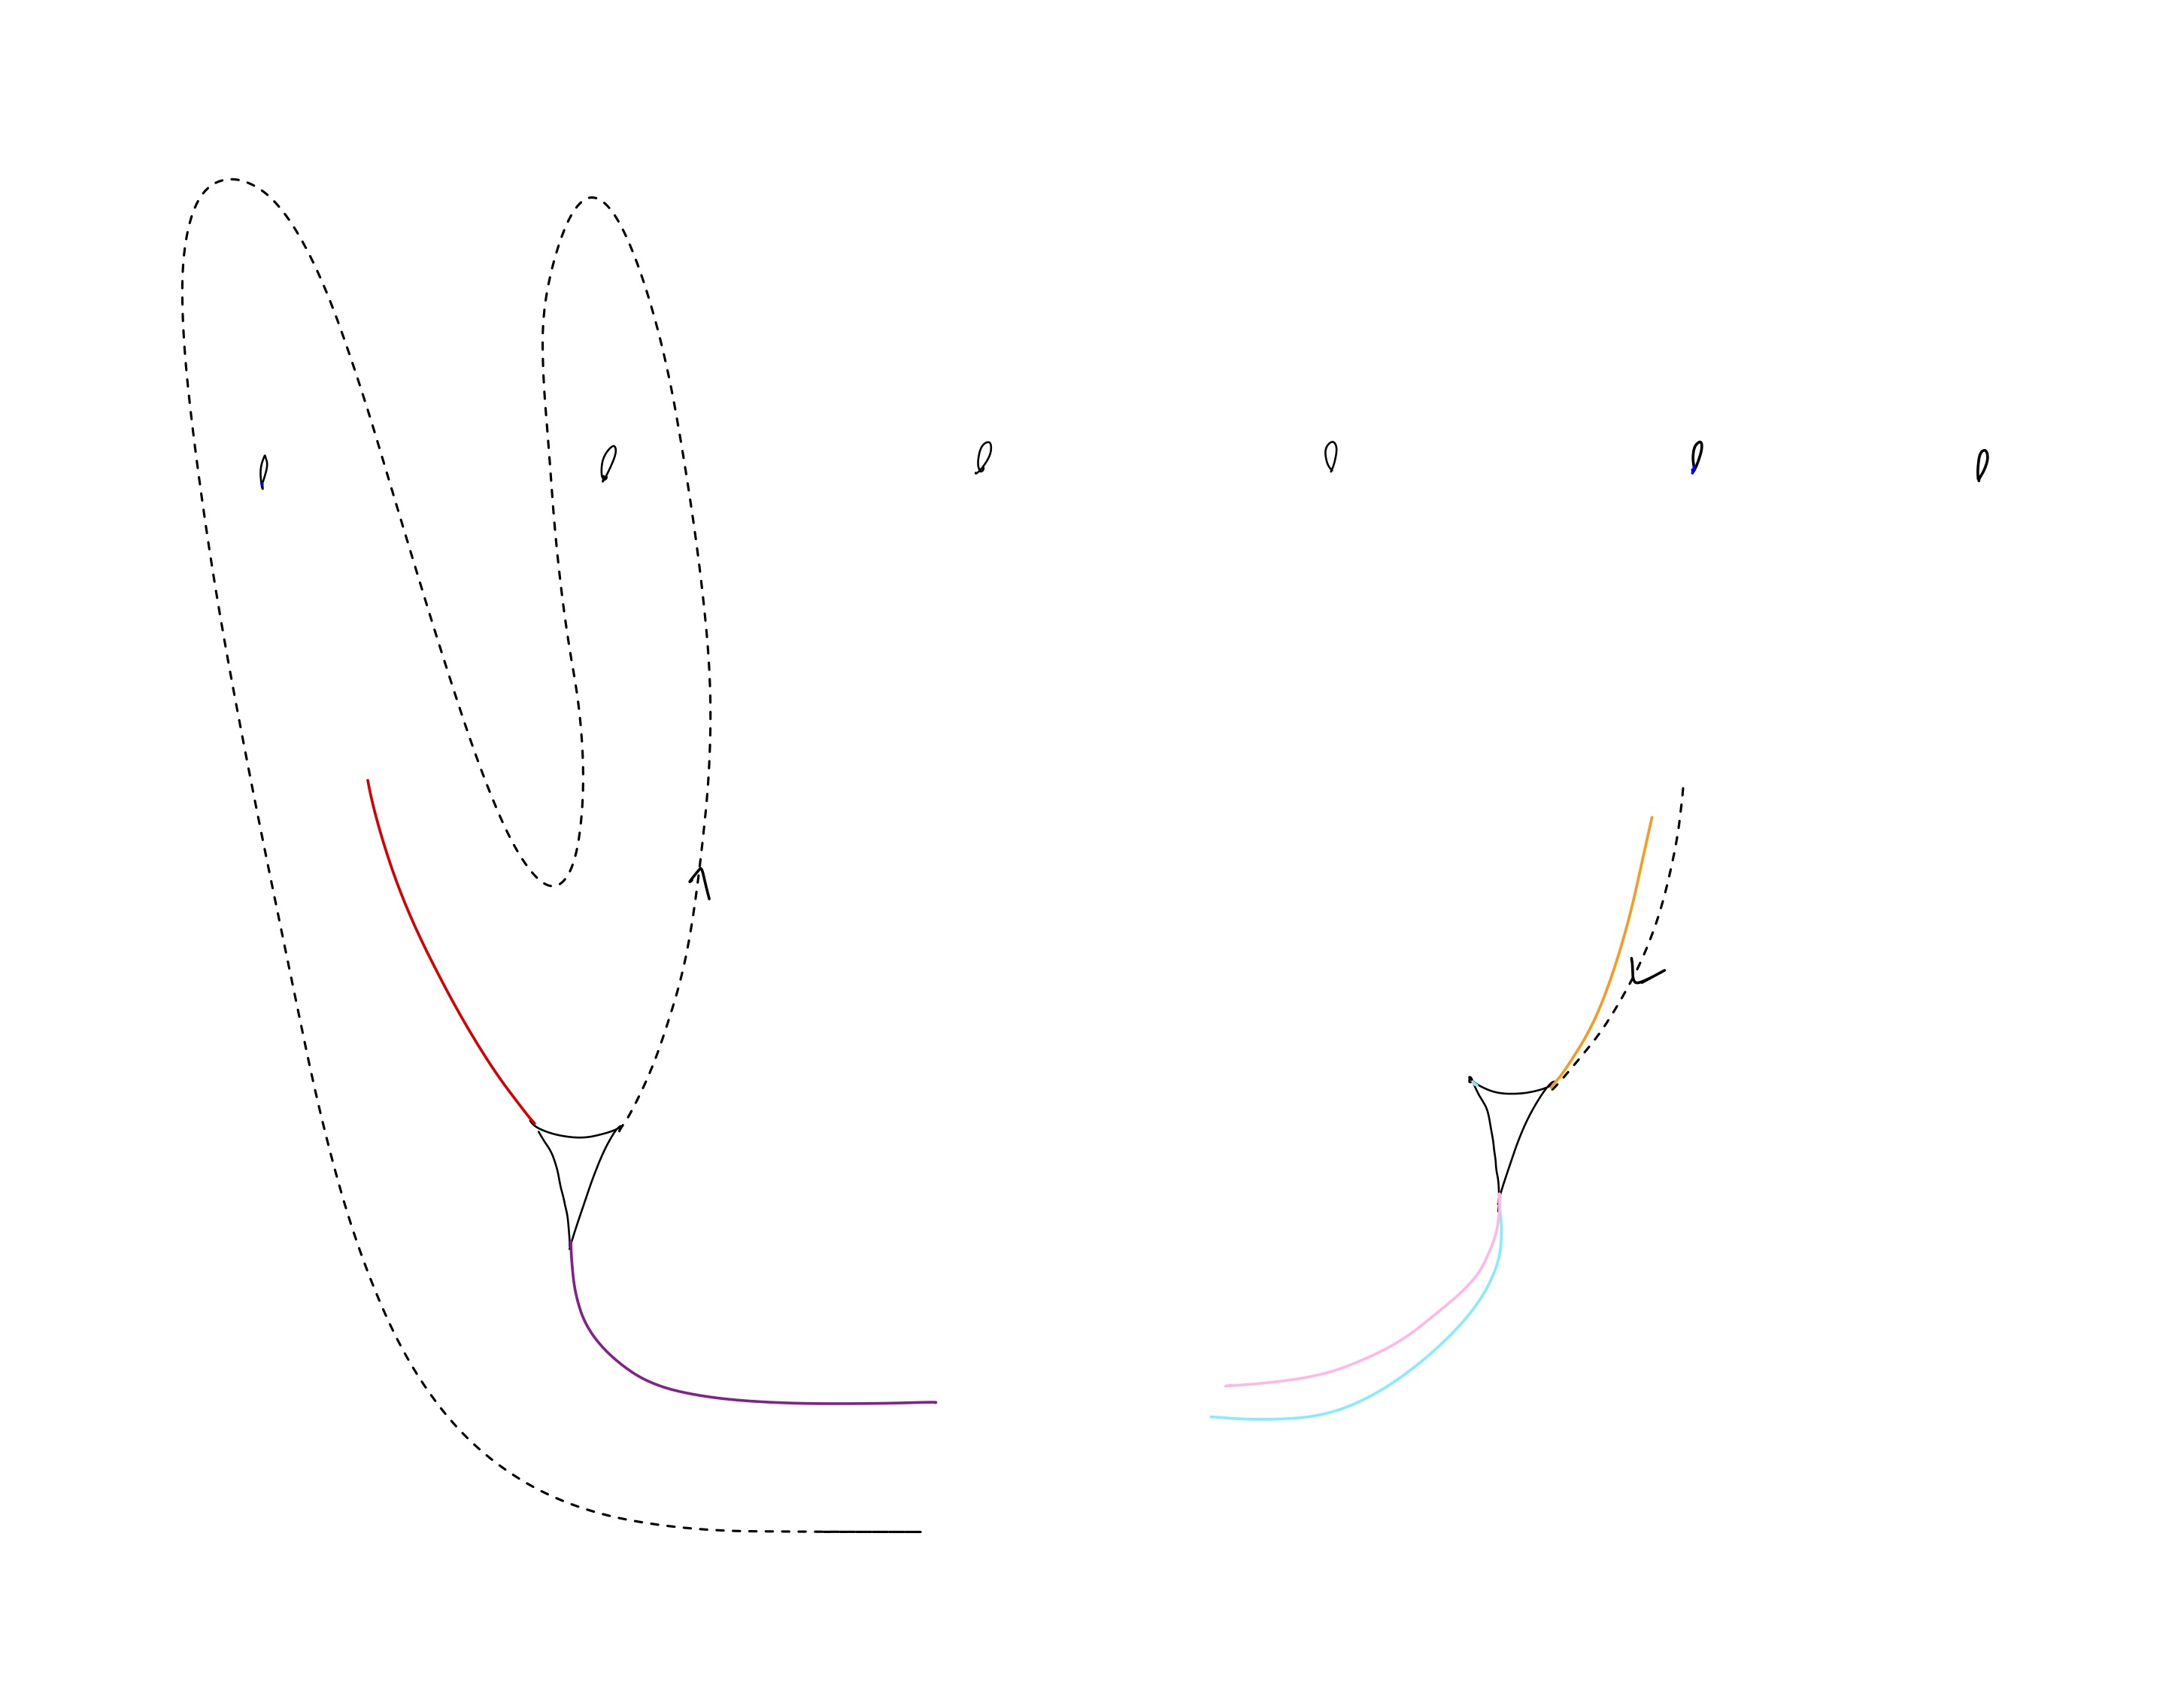
\includegraphics[width=\linewidth]{figures_case_analysis/track17_case_analysis/VSF.jpg}
    \caption{VSF1}
    \label{fig:VSF1}
\end{figure}

\begin{figure}[ht]
    \centering
    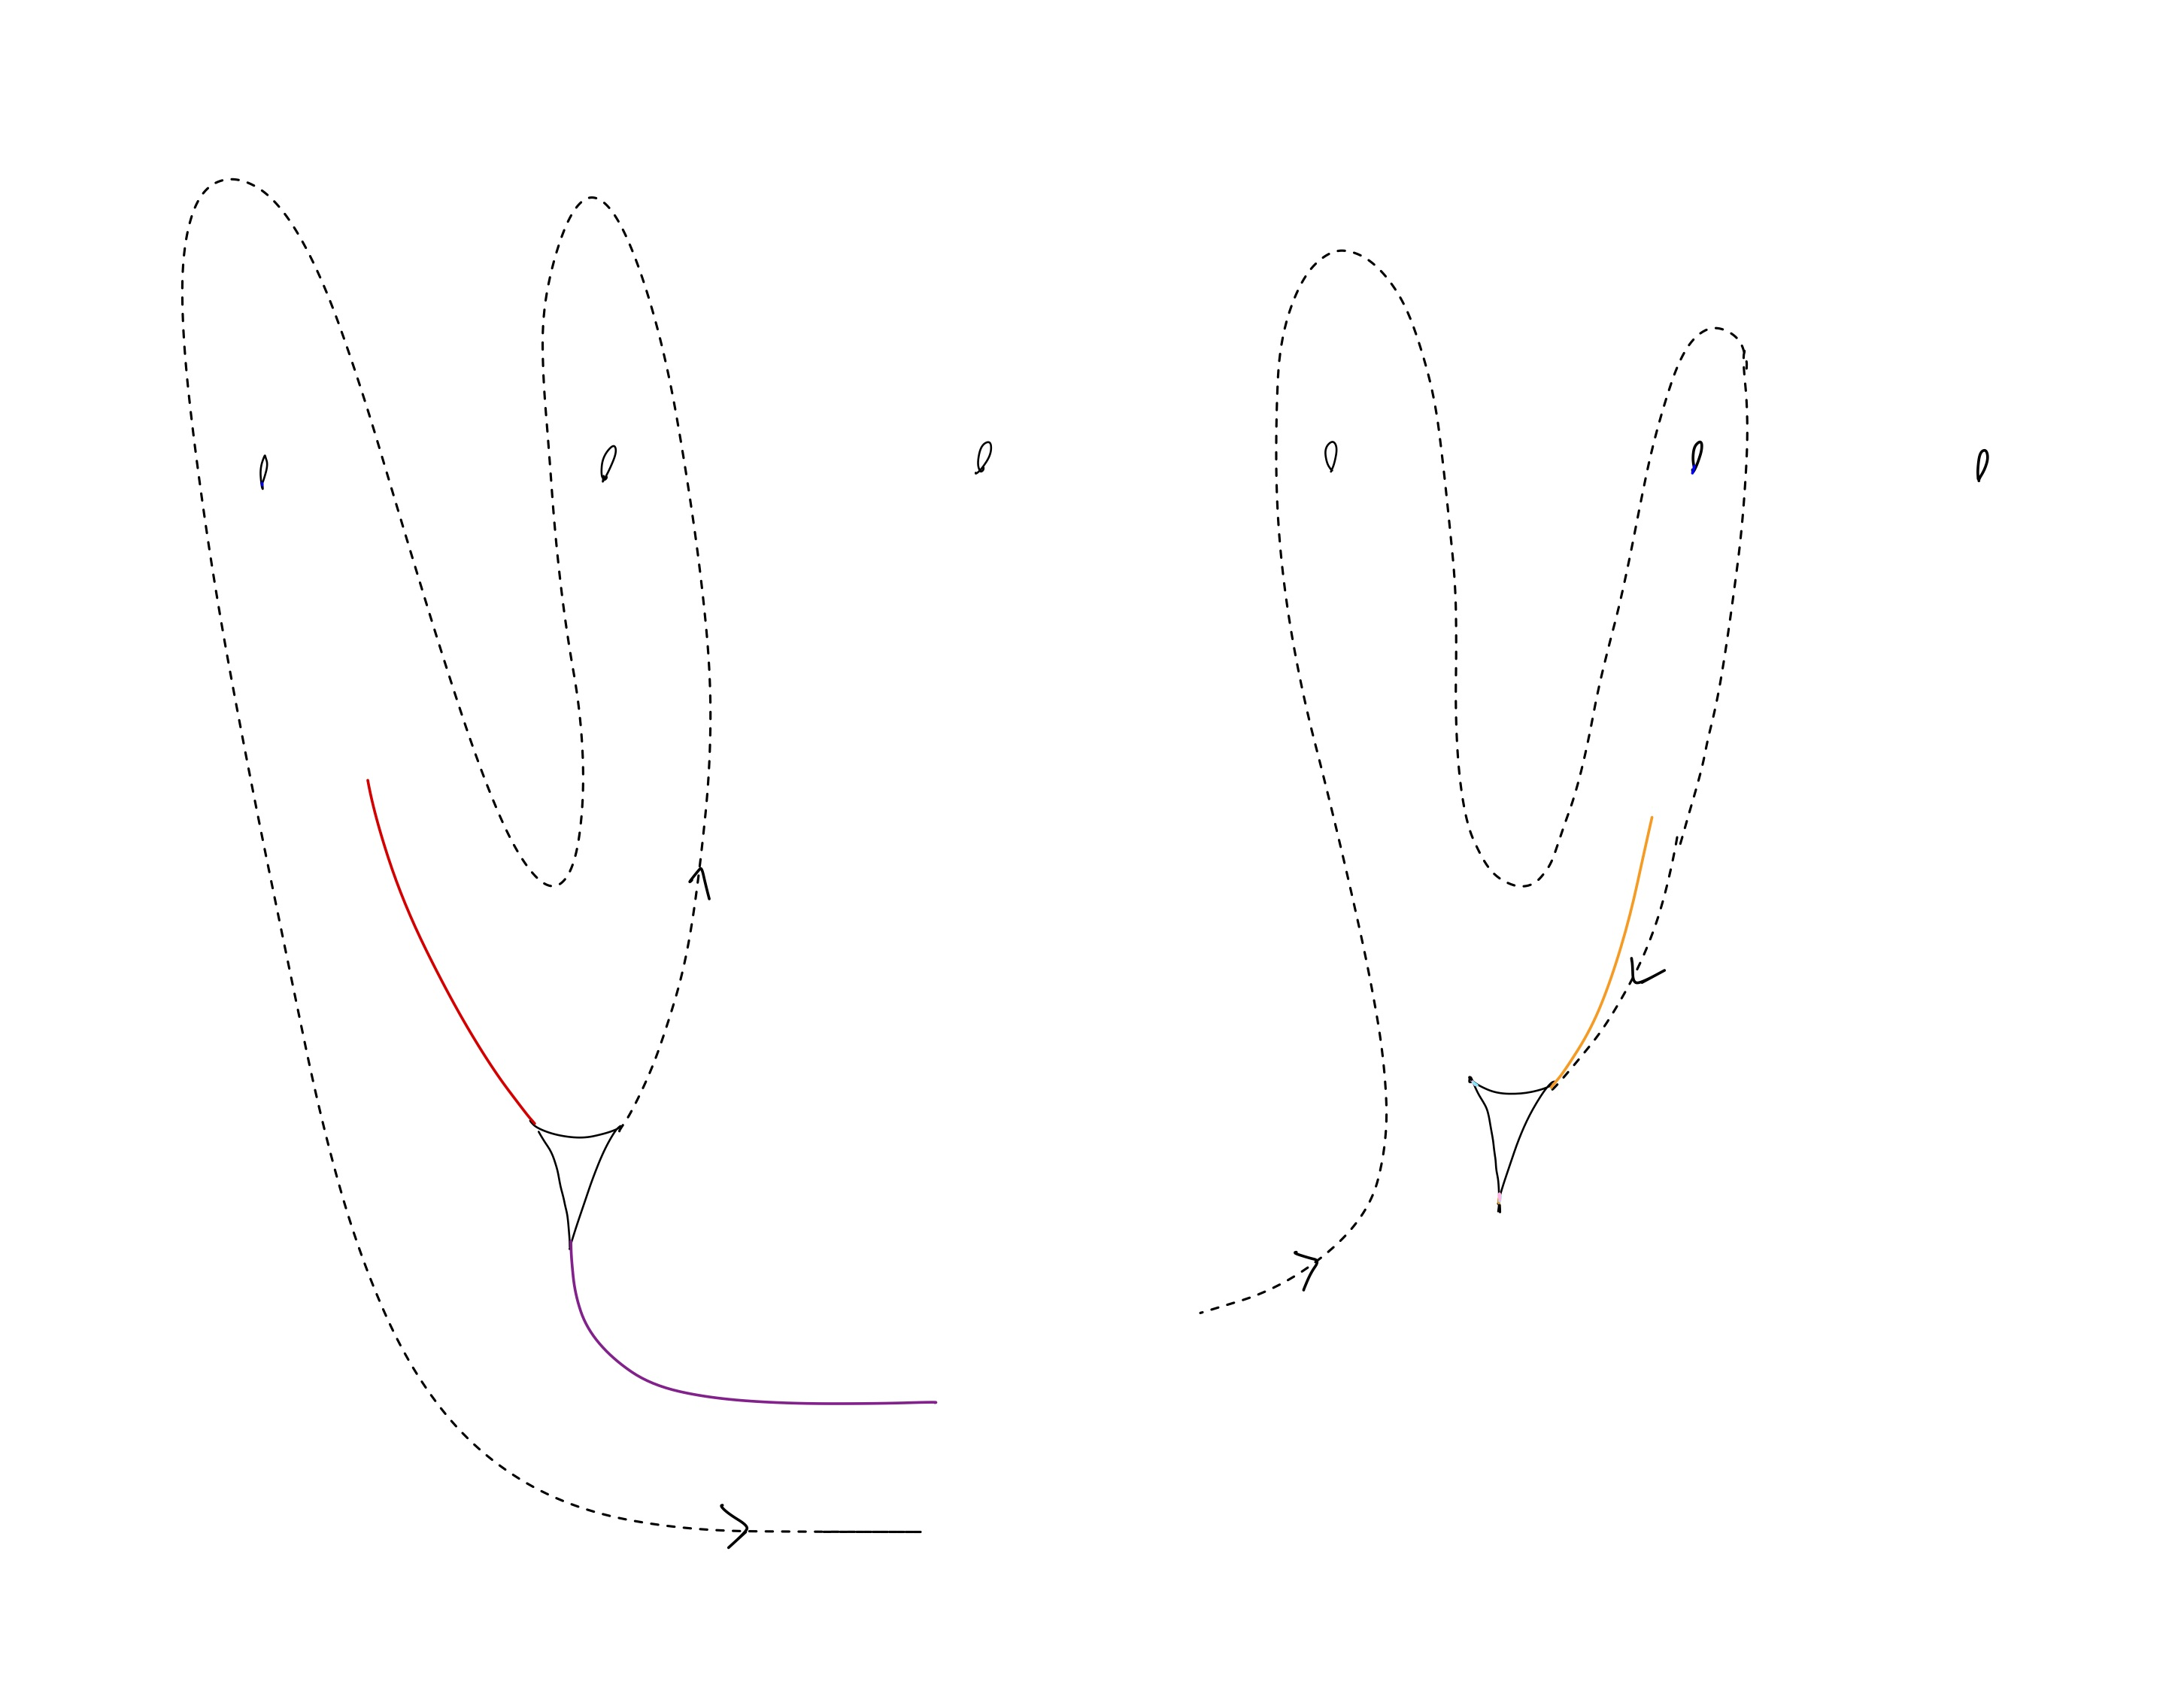
\includegraphics[width=\linewidth]{figures_case_analysis/track17_case_analysis/Bawn-1.jpg}
    \caption{Bawn1}
    \label{fig:Bawn1}
\end{figure}

\begin{figure}[ht]
    \centering
    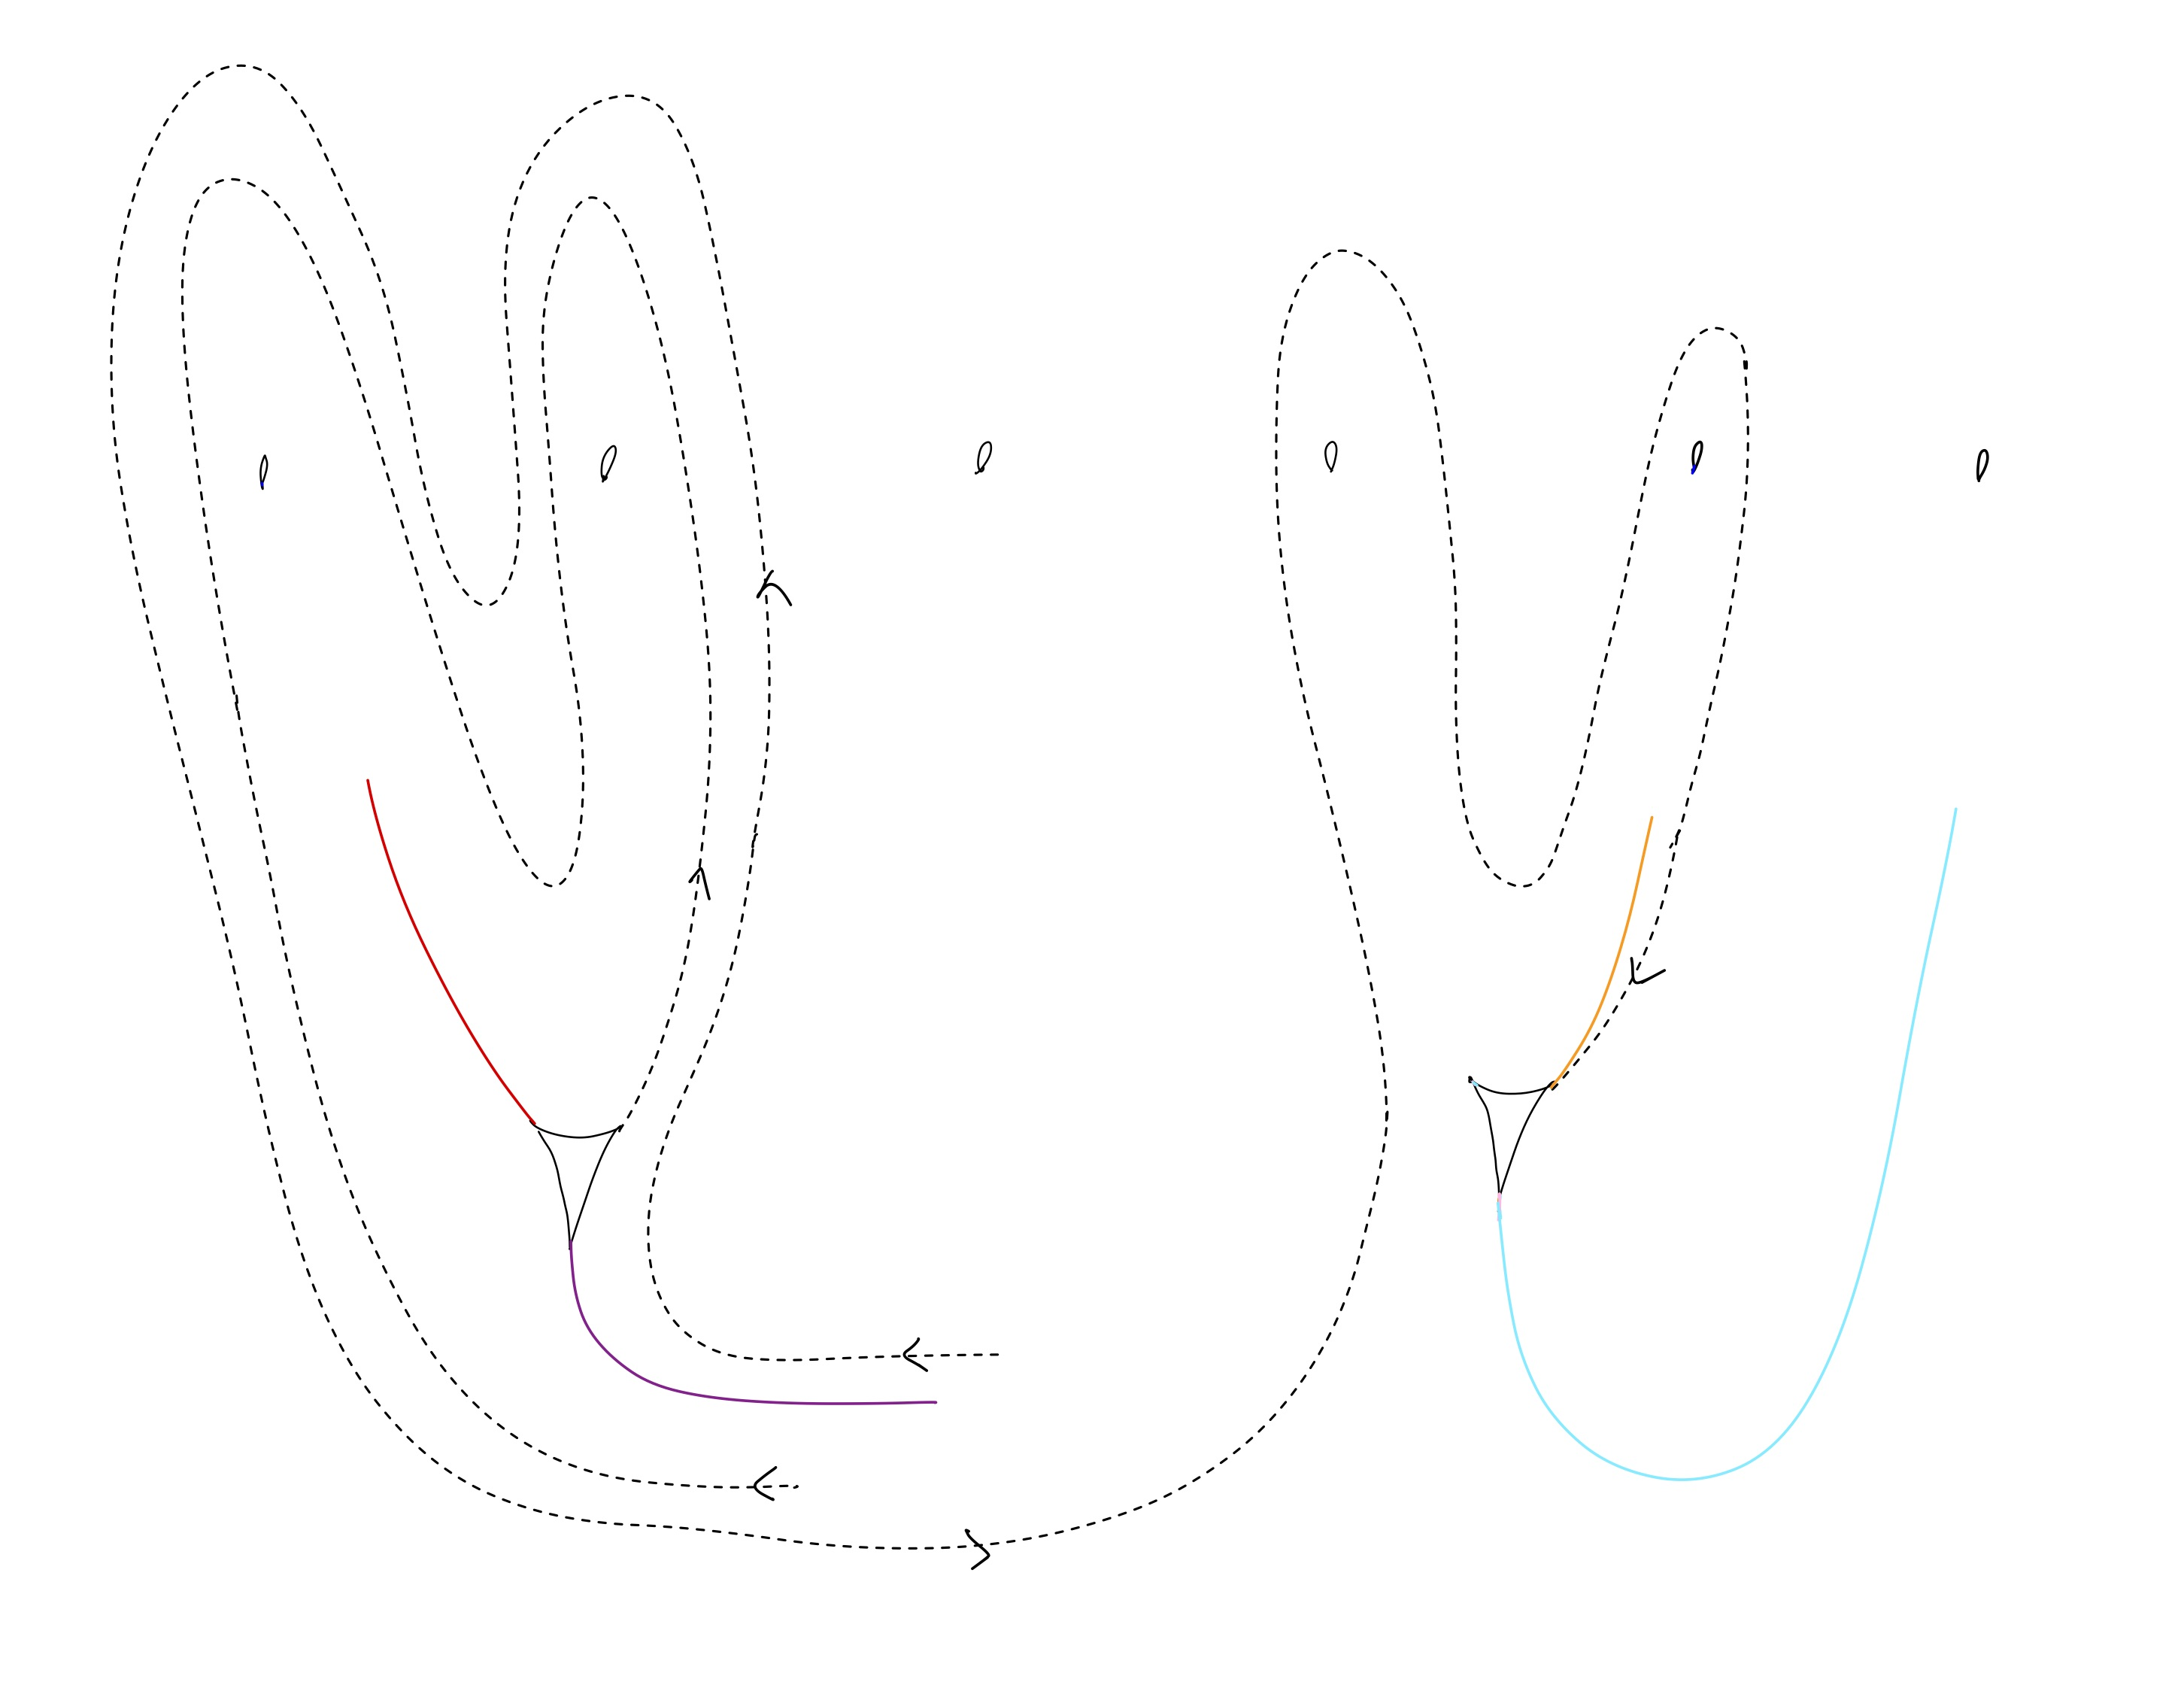
\includegraphics[width=\linewidth]{figures_case_analysis/track17_case_analysis/Bawn-2.jpg}
    \caption{Bawn2}
    \label{fig:Bawn2}
\end{figure}

\begin{figure}[ht]
    \centering
    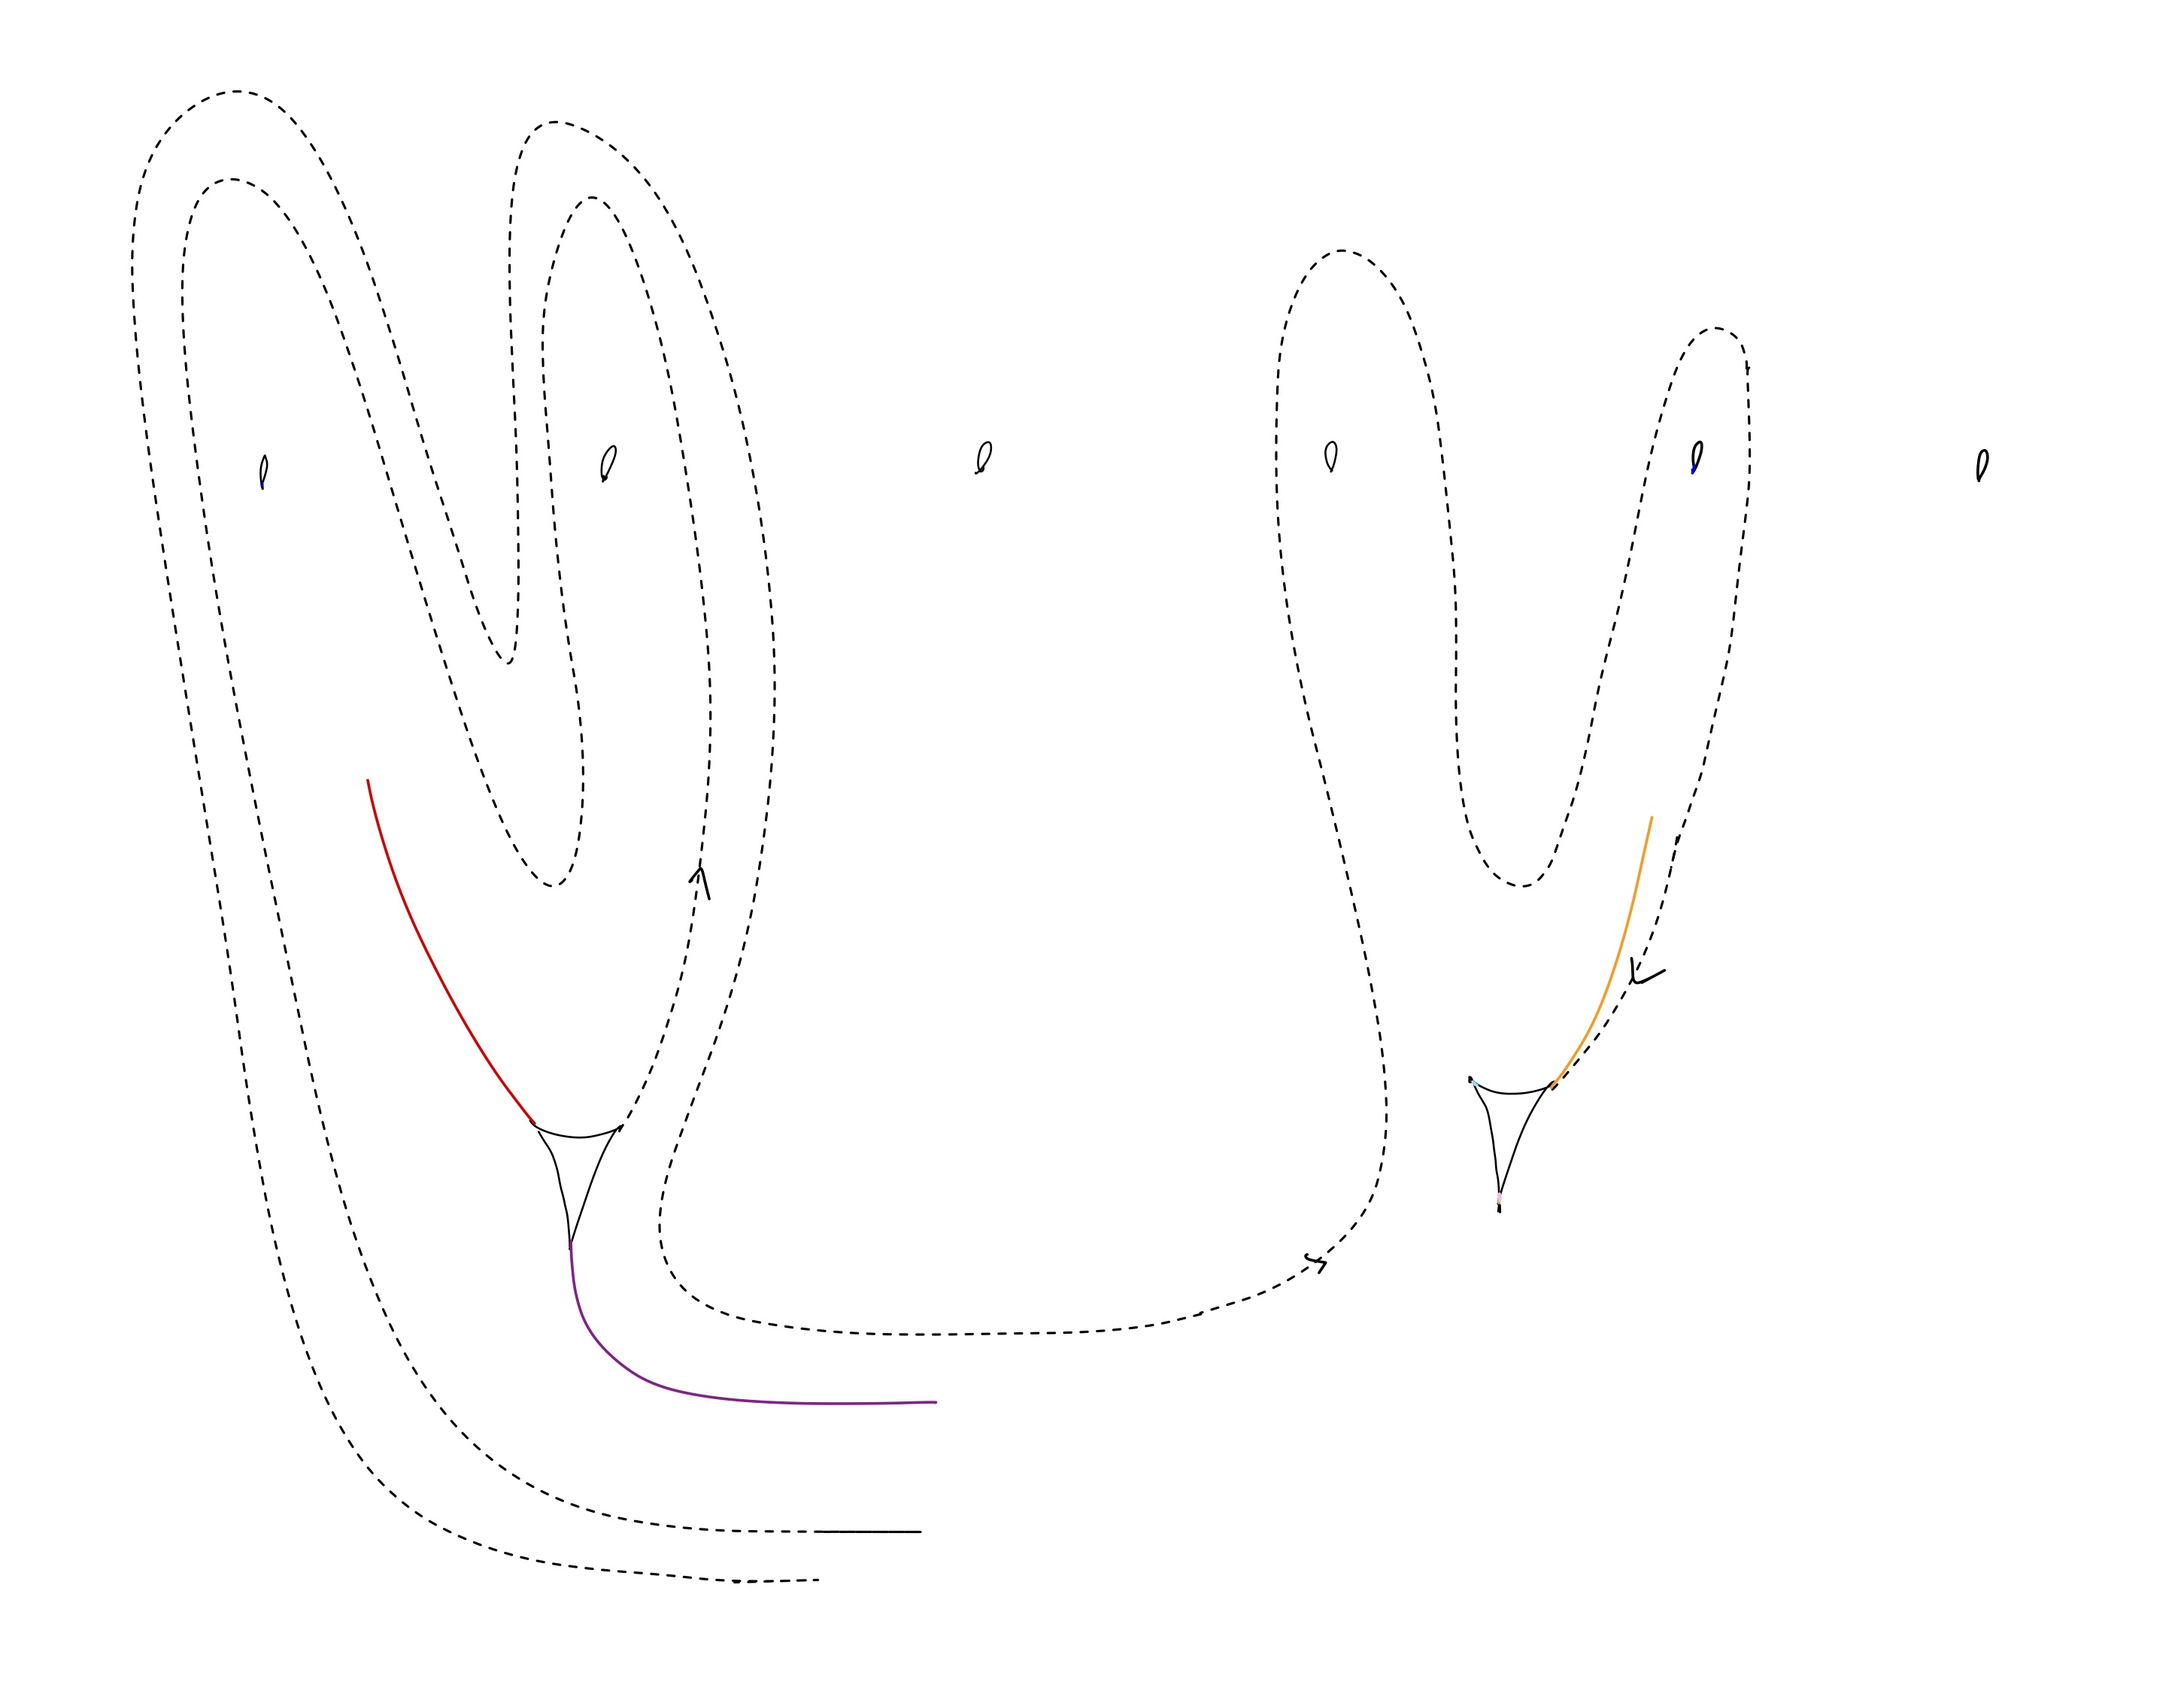
\includegraphics[width=\linewidth]{figures_case_analysis/track17_case_analysis/Bawn-3.jpg}
    \caption{Bawn3}
    \label{fig:Bawn3}
\end{figure}

\begin{figure}[ht]
    \centering
    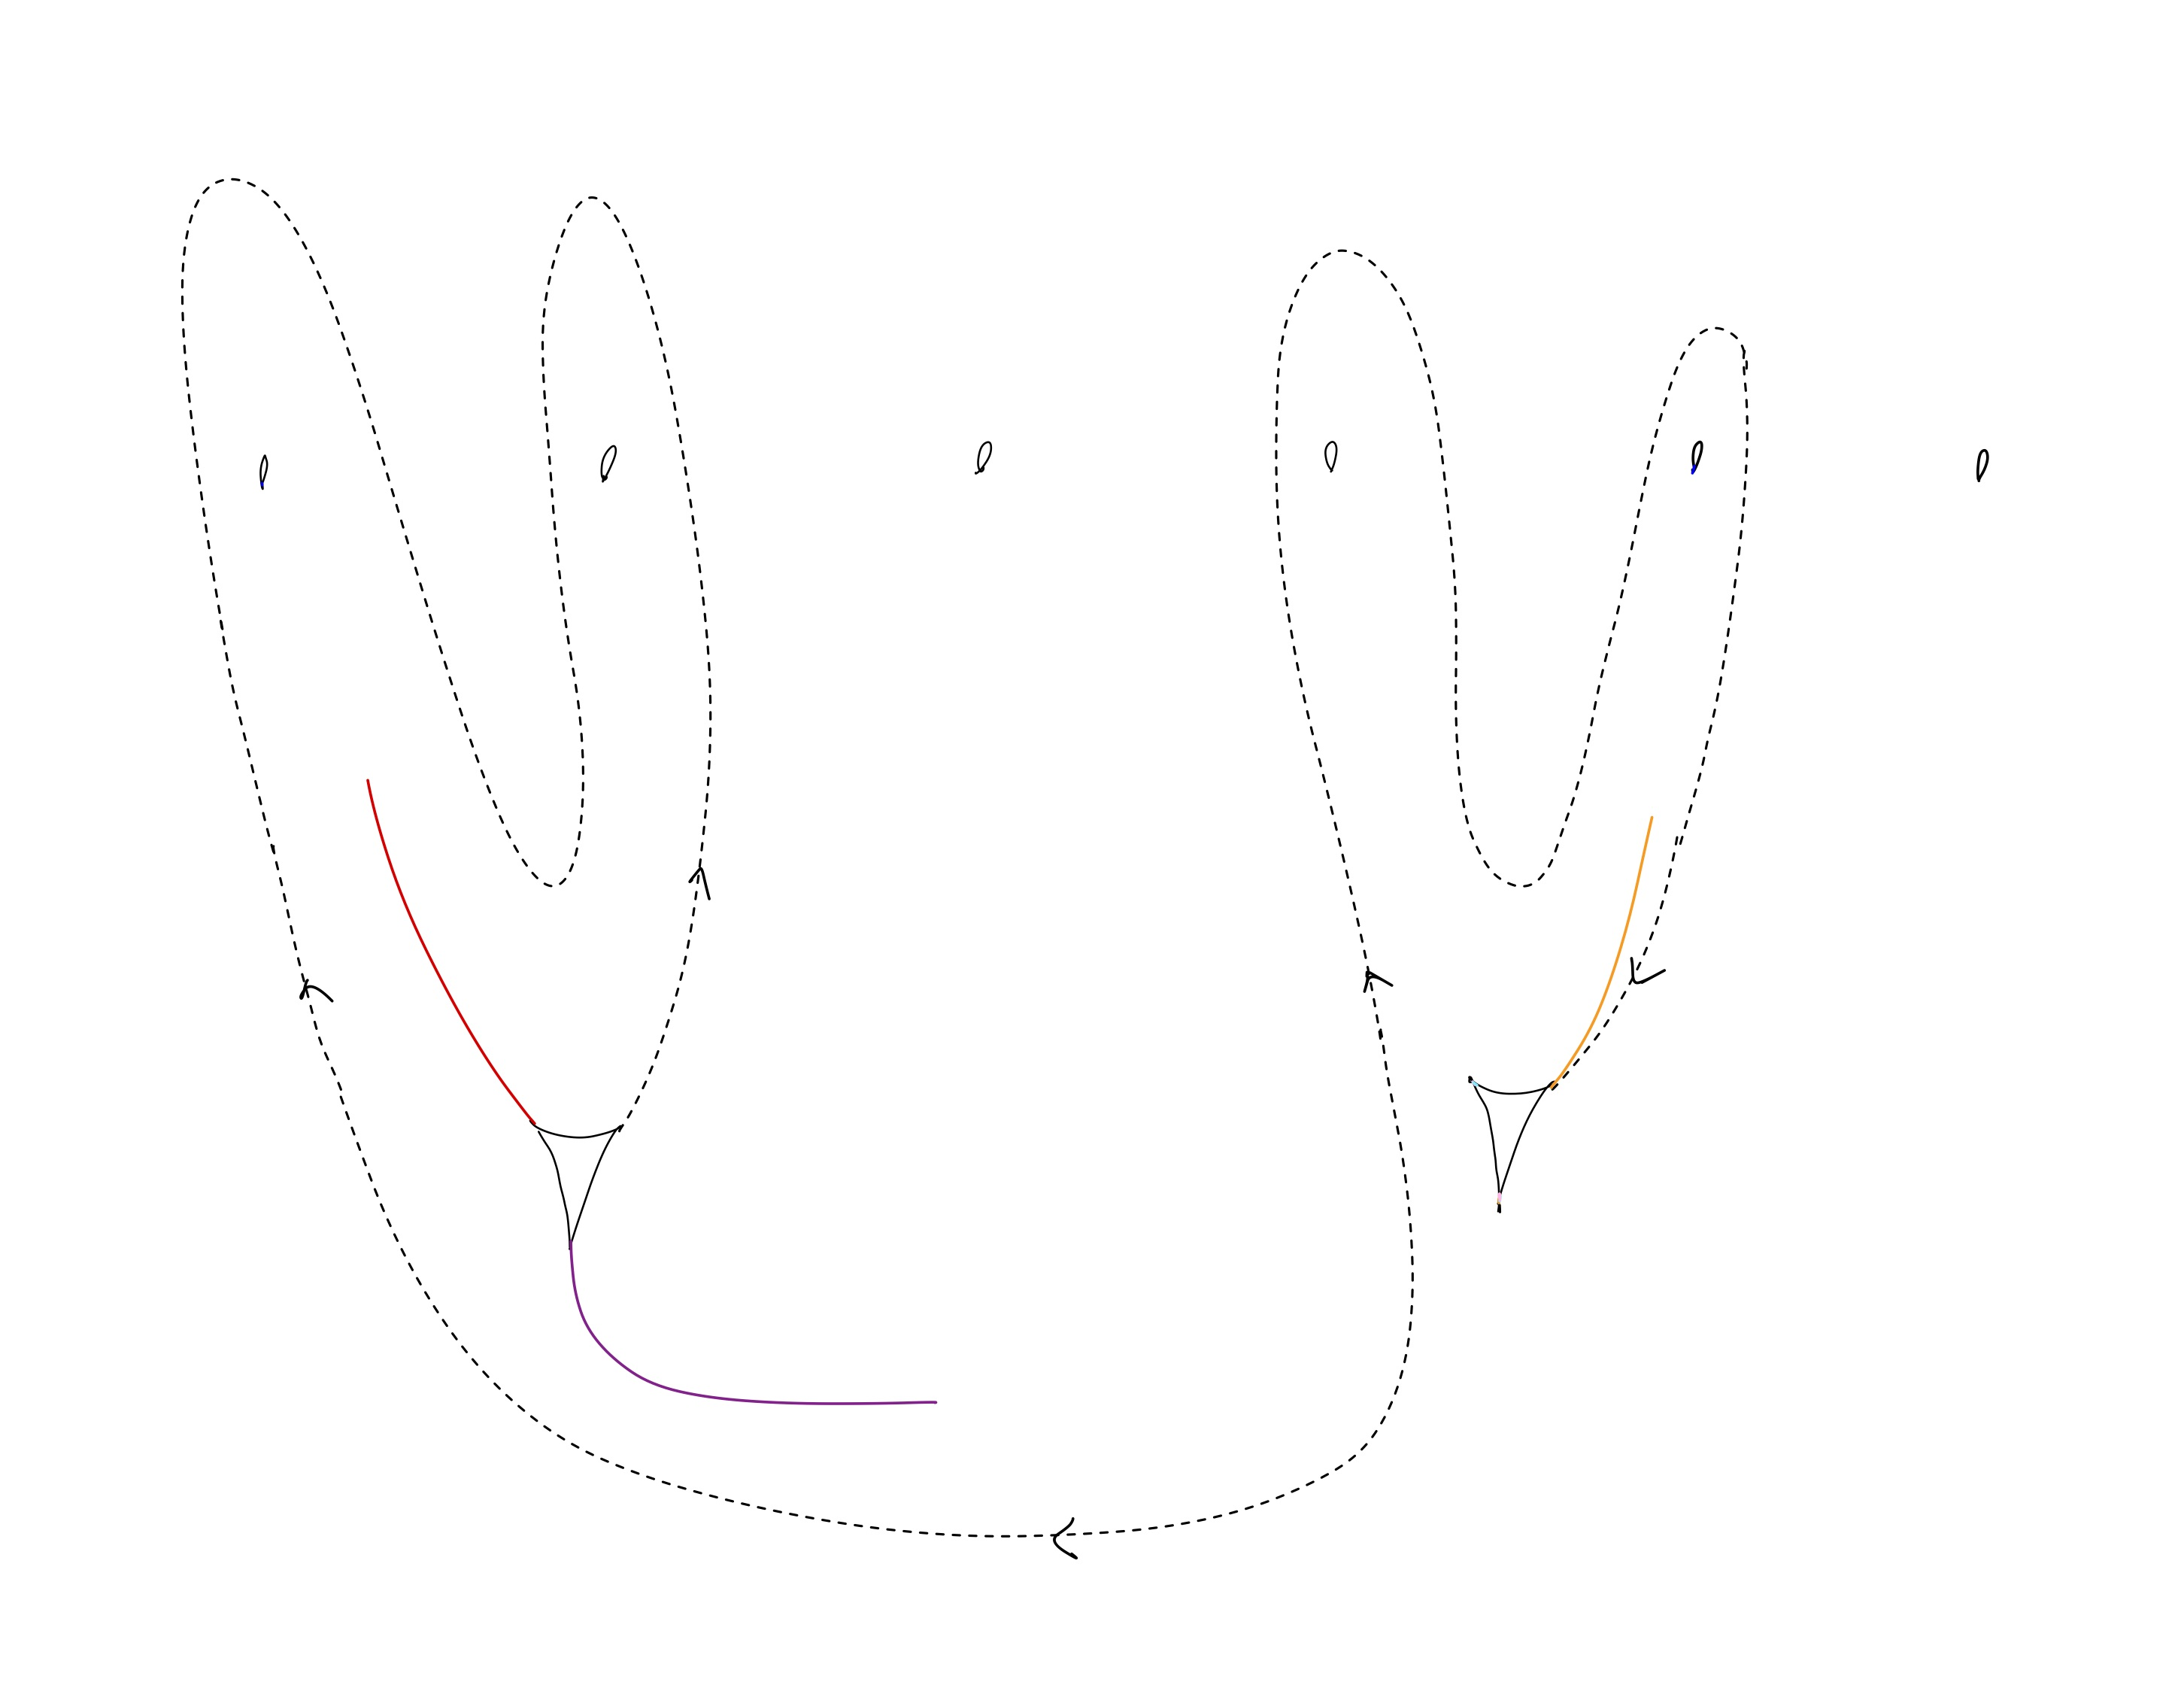
\includegraphics[width=\linewidth]{figures_case_analysis/track17_case_analysis/Bawn-4.jpg}
    \caption{Bawn4}
    \label{fig:Bawn4}
\end{figure}
\clearpage

\begin{figure}[ht]
    \centering
    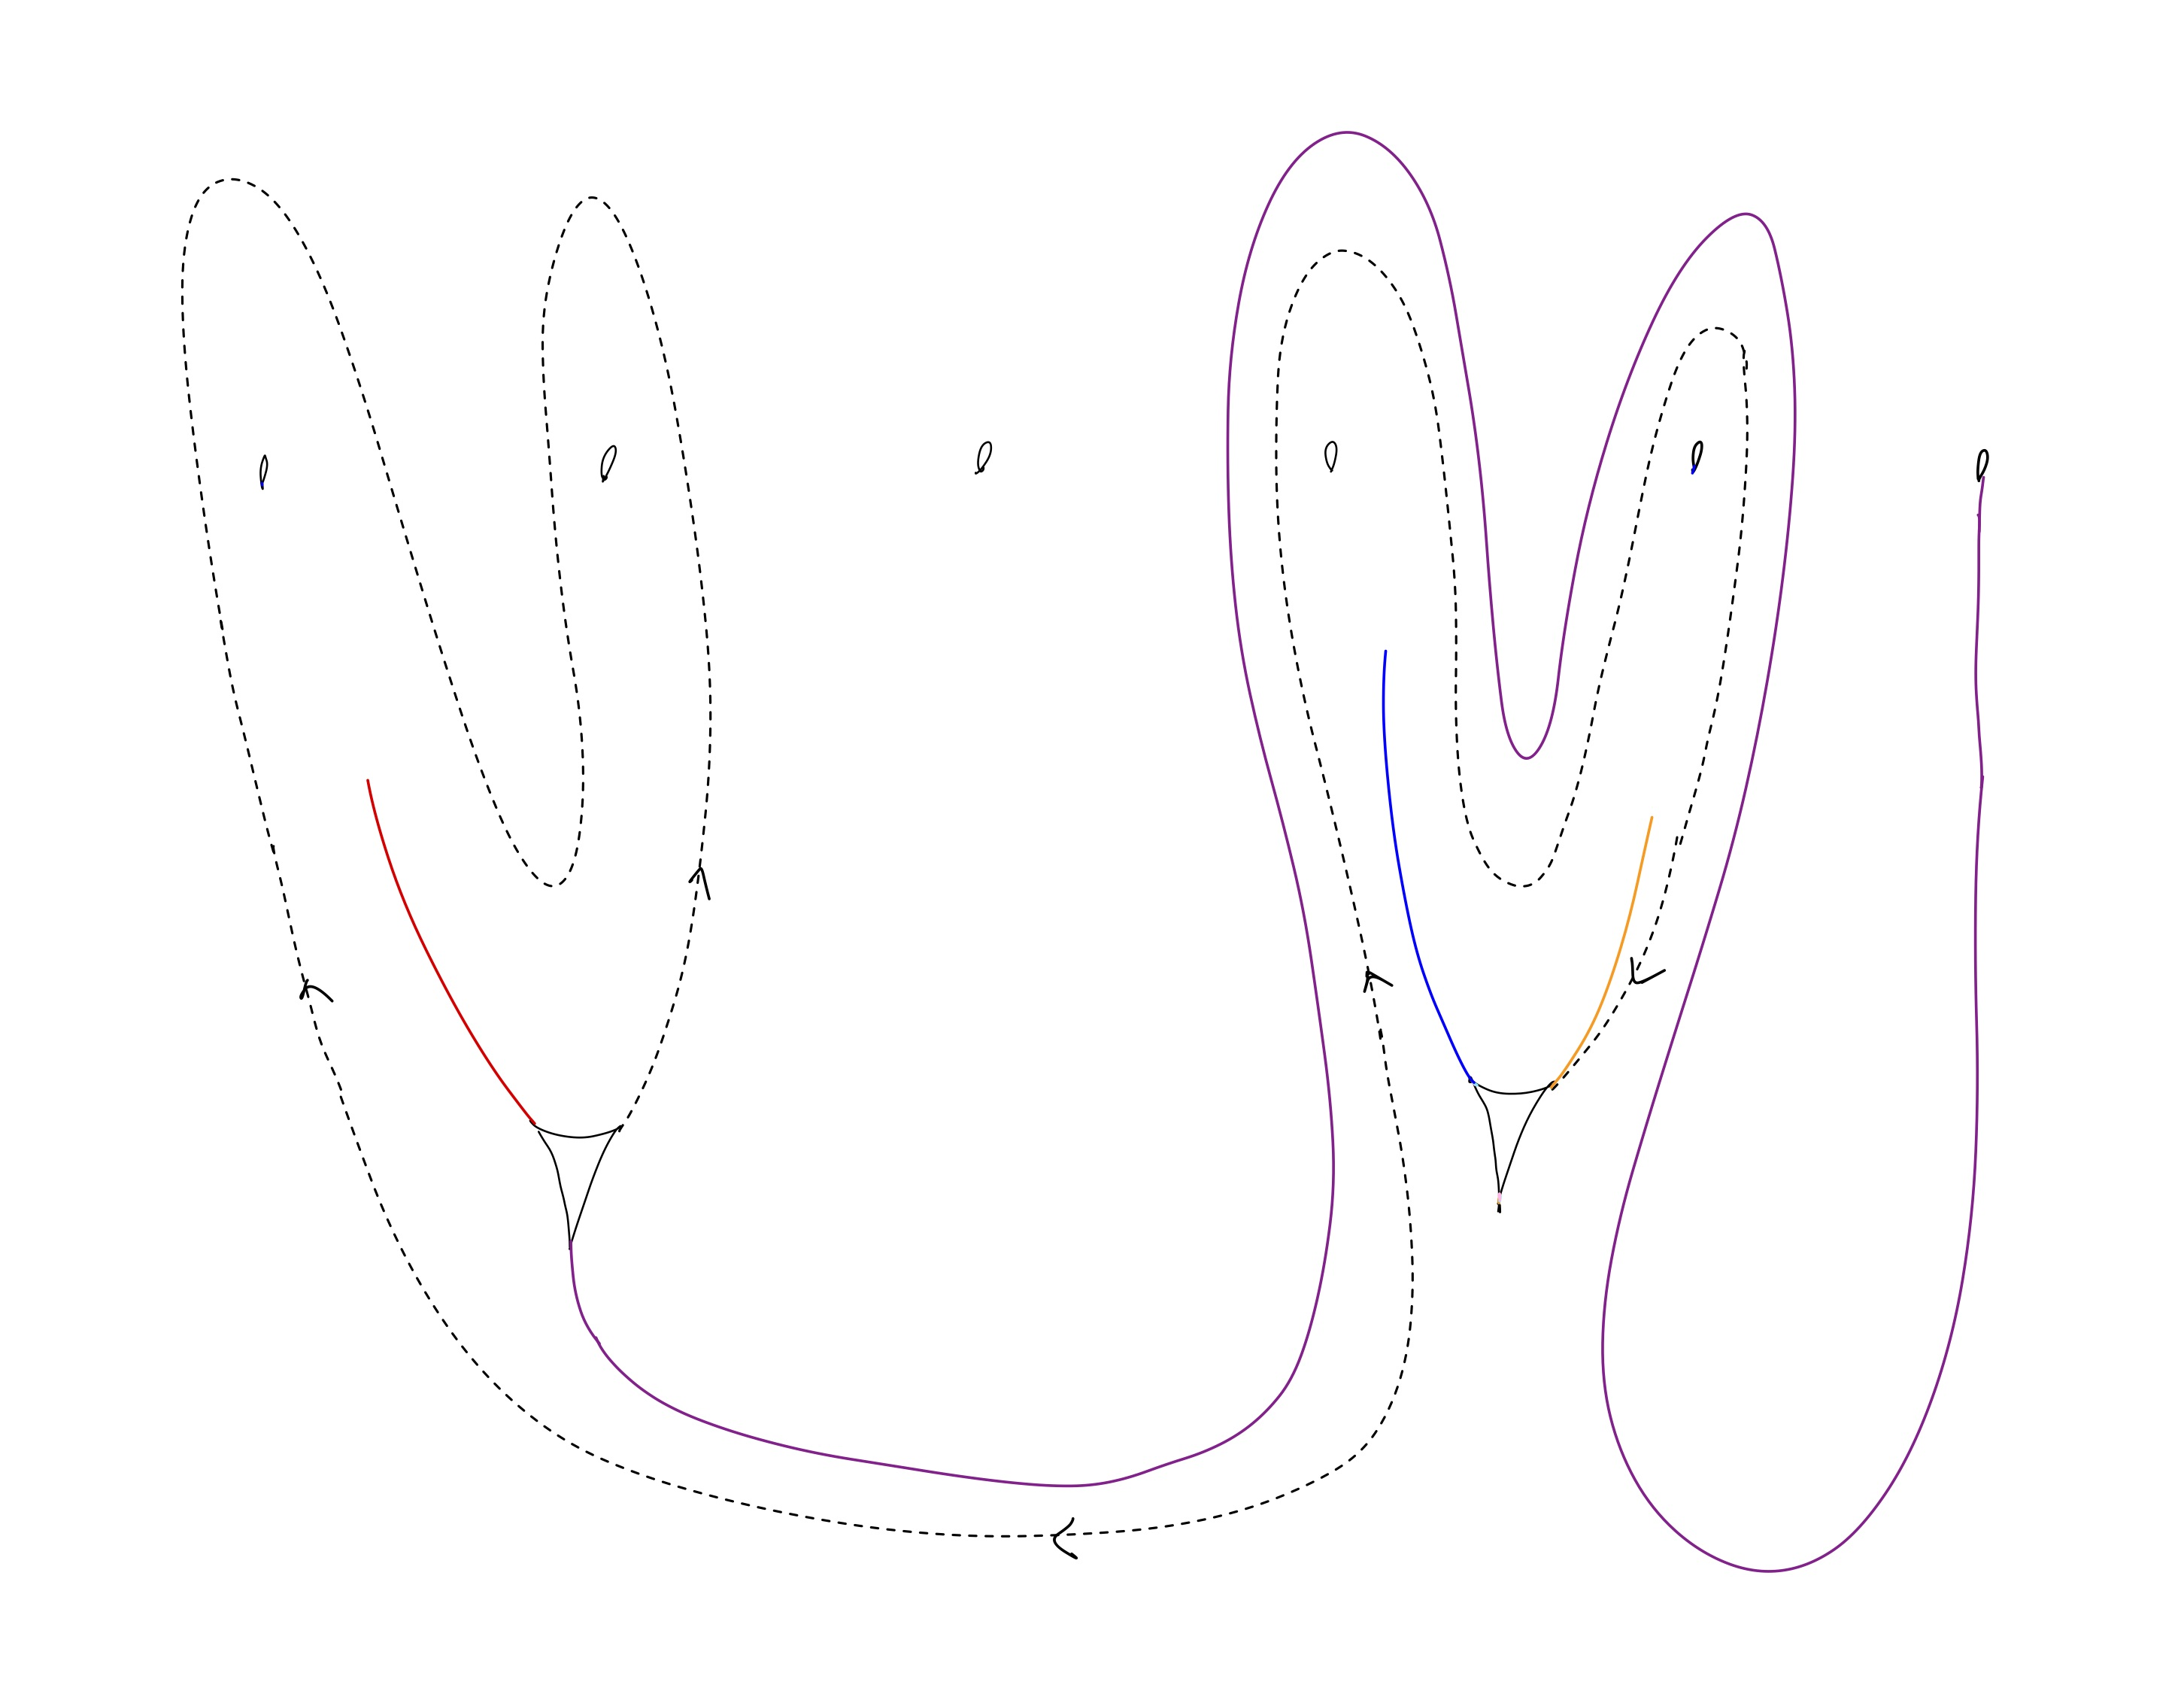
\includegraphics[width=\linewidth]{figures_case_analysis/track17_case_analysis/Blore-1.jpg}
    \caption{Blore1}
    \label{fig:Blore1}
\end{figure}

\begin{figure}[ht]
    \centering
    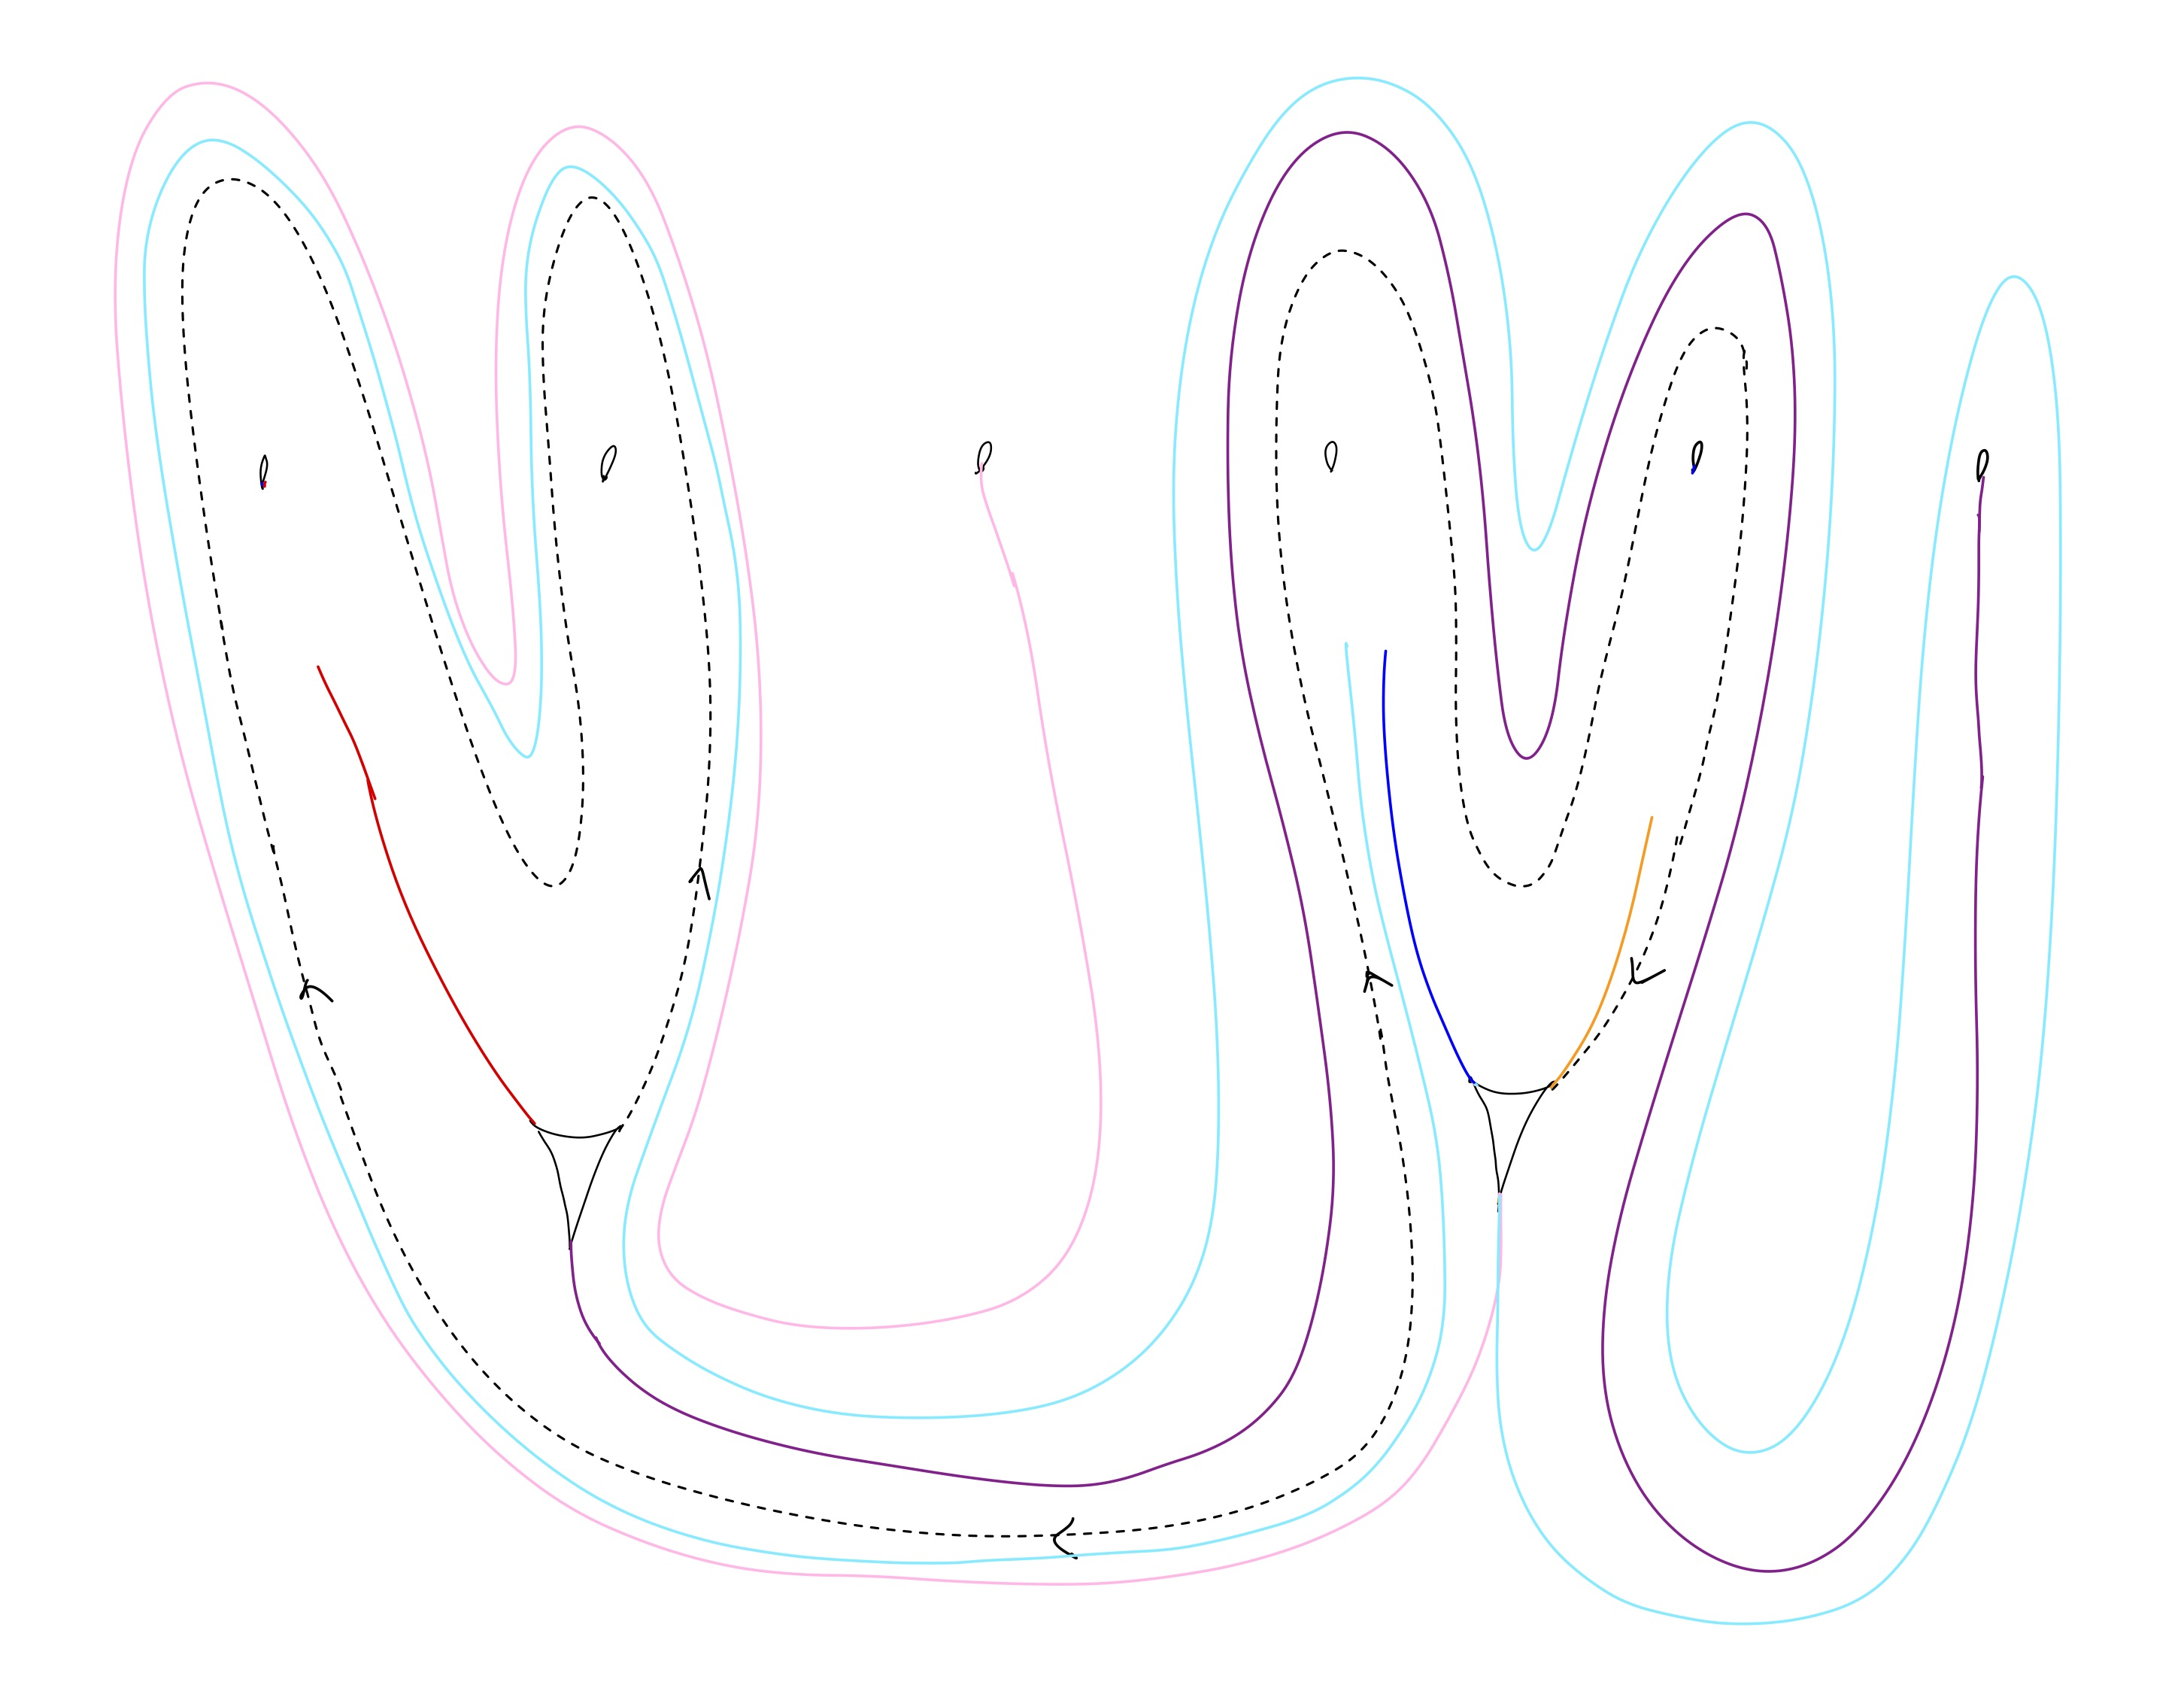
\includegraphics[width=\linewidth]{figures_case_analysis/track17_case_analysis/Blore-2.jpg}
    \caption{Blore2}
    \label{fig:Blore2}
\end{figure}

\begin{figure}[ht]
    \centering
    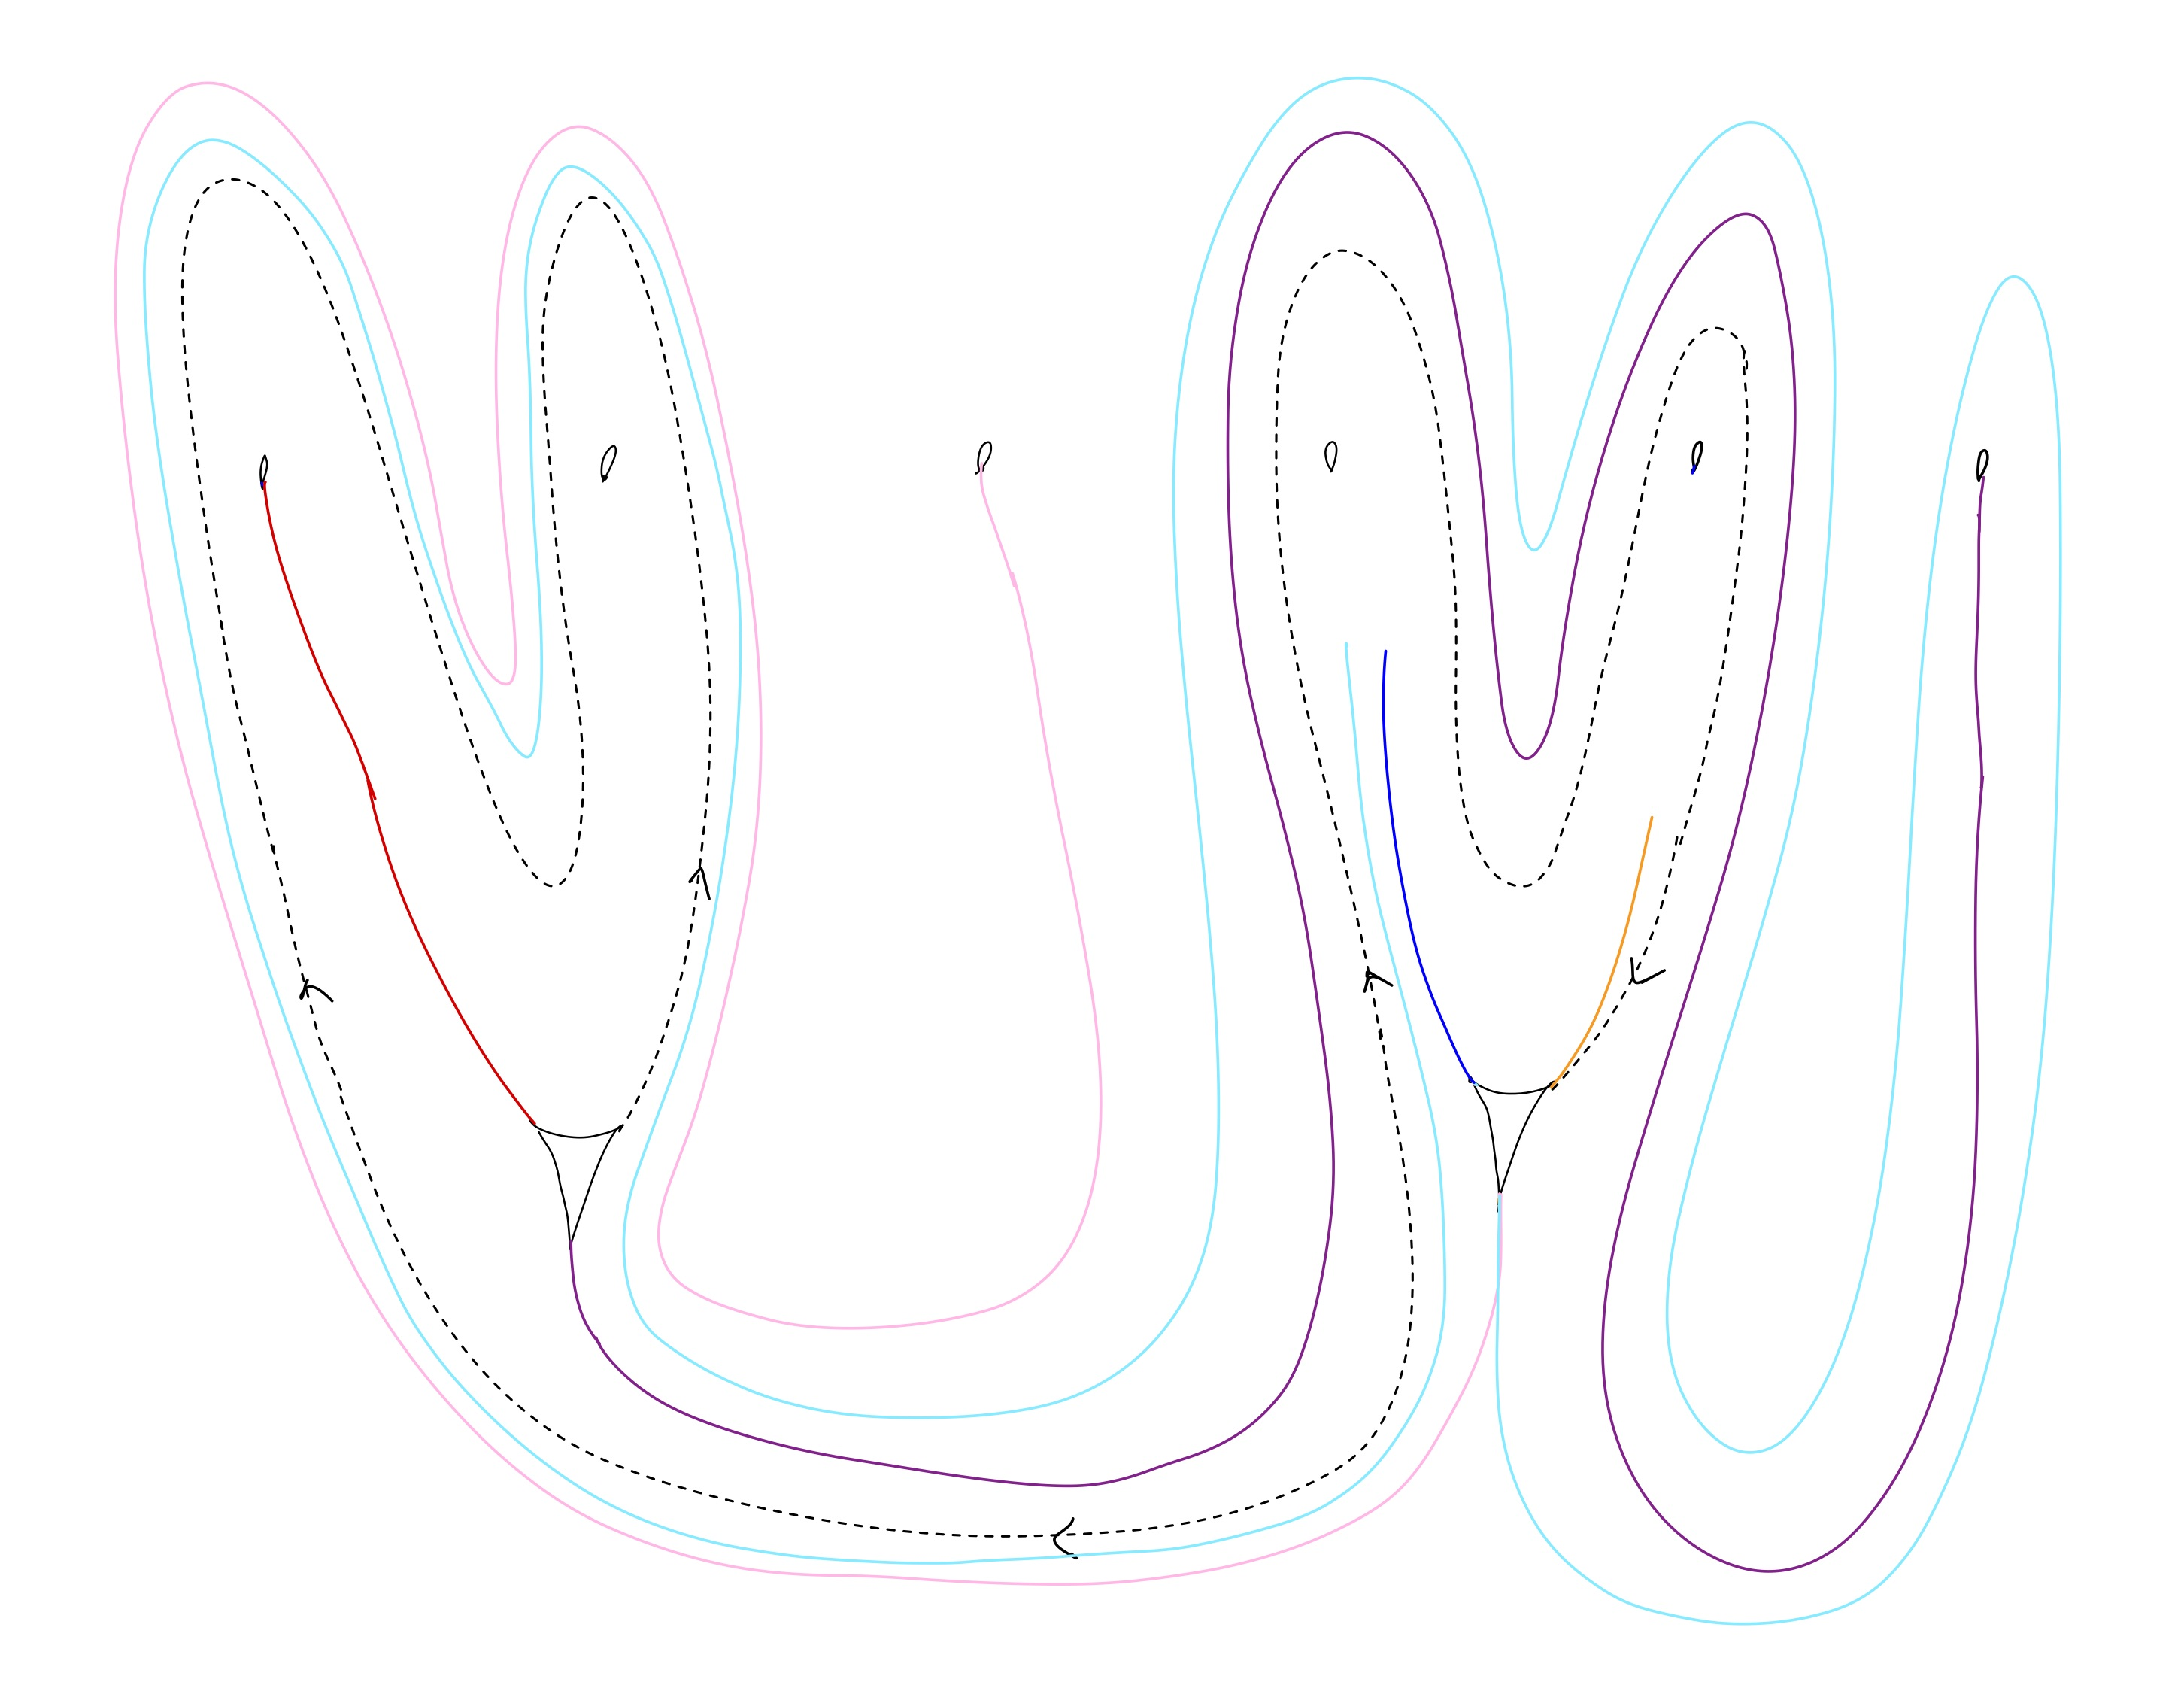
\includegraphics[width=\linewidth]{figures_case_analysis/track17_case_analysis/Blore-3.jpg}
    \caption{Blore3}
    \label{fig:Blore3}
\end{figure}

\begin{figure}[ht]
    \centering
    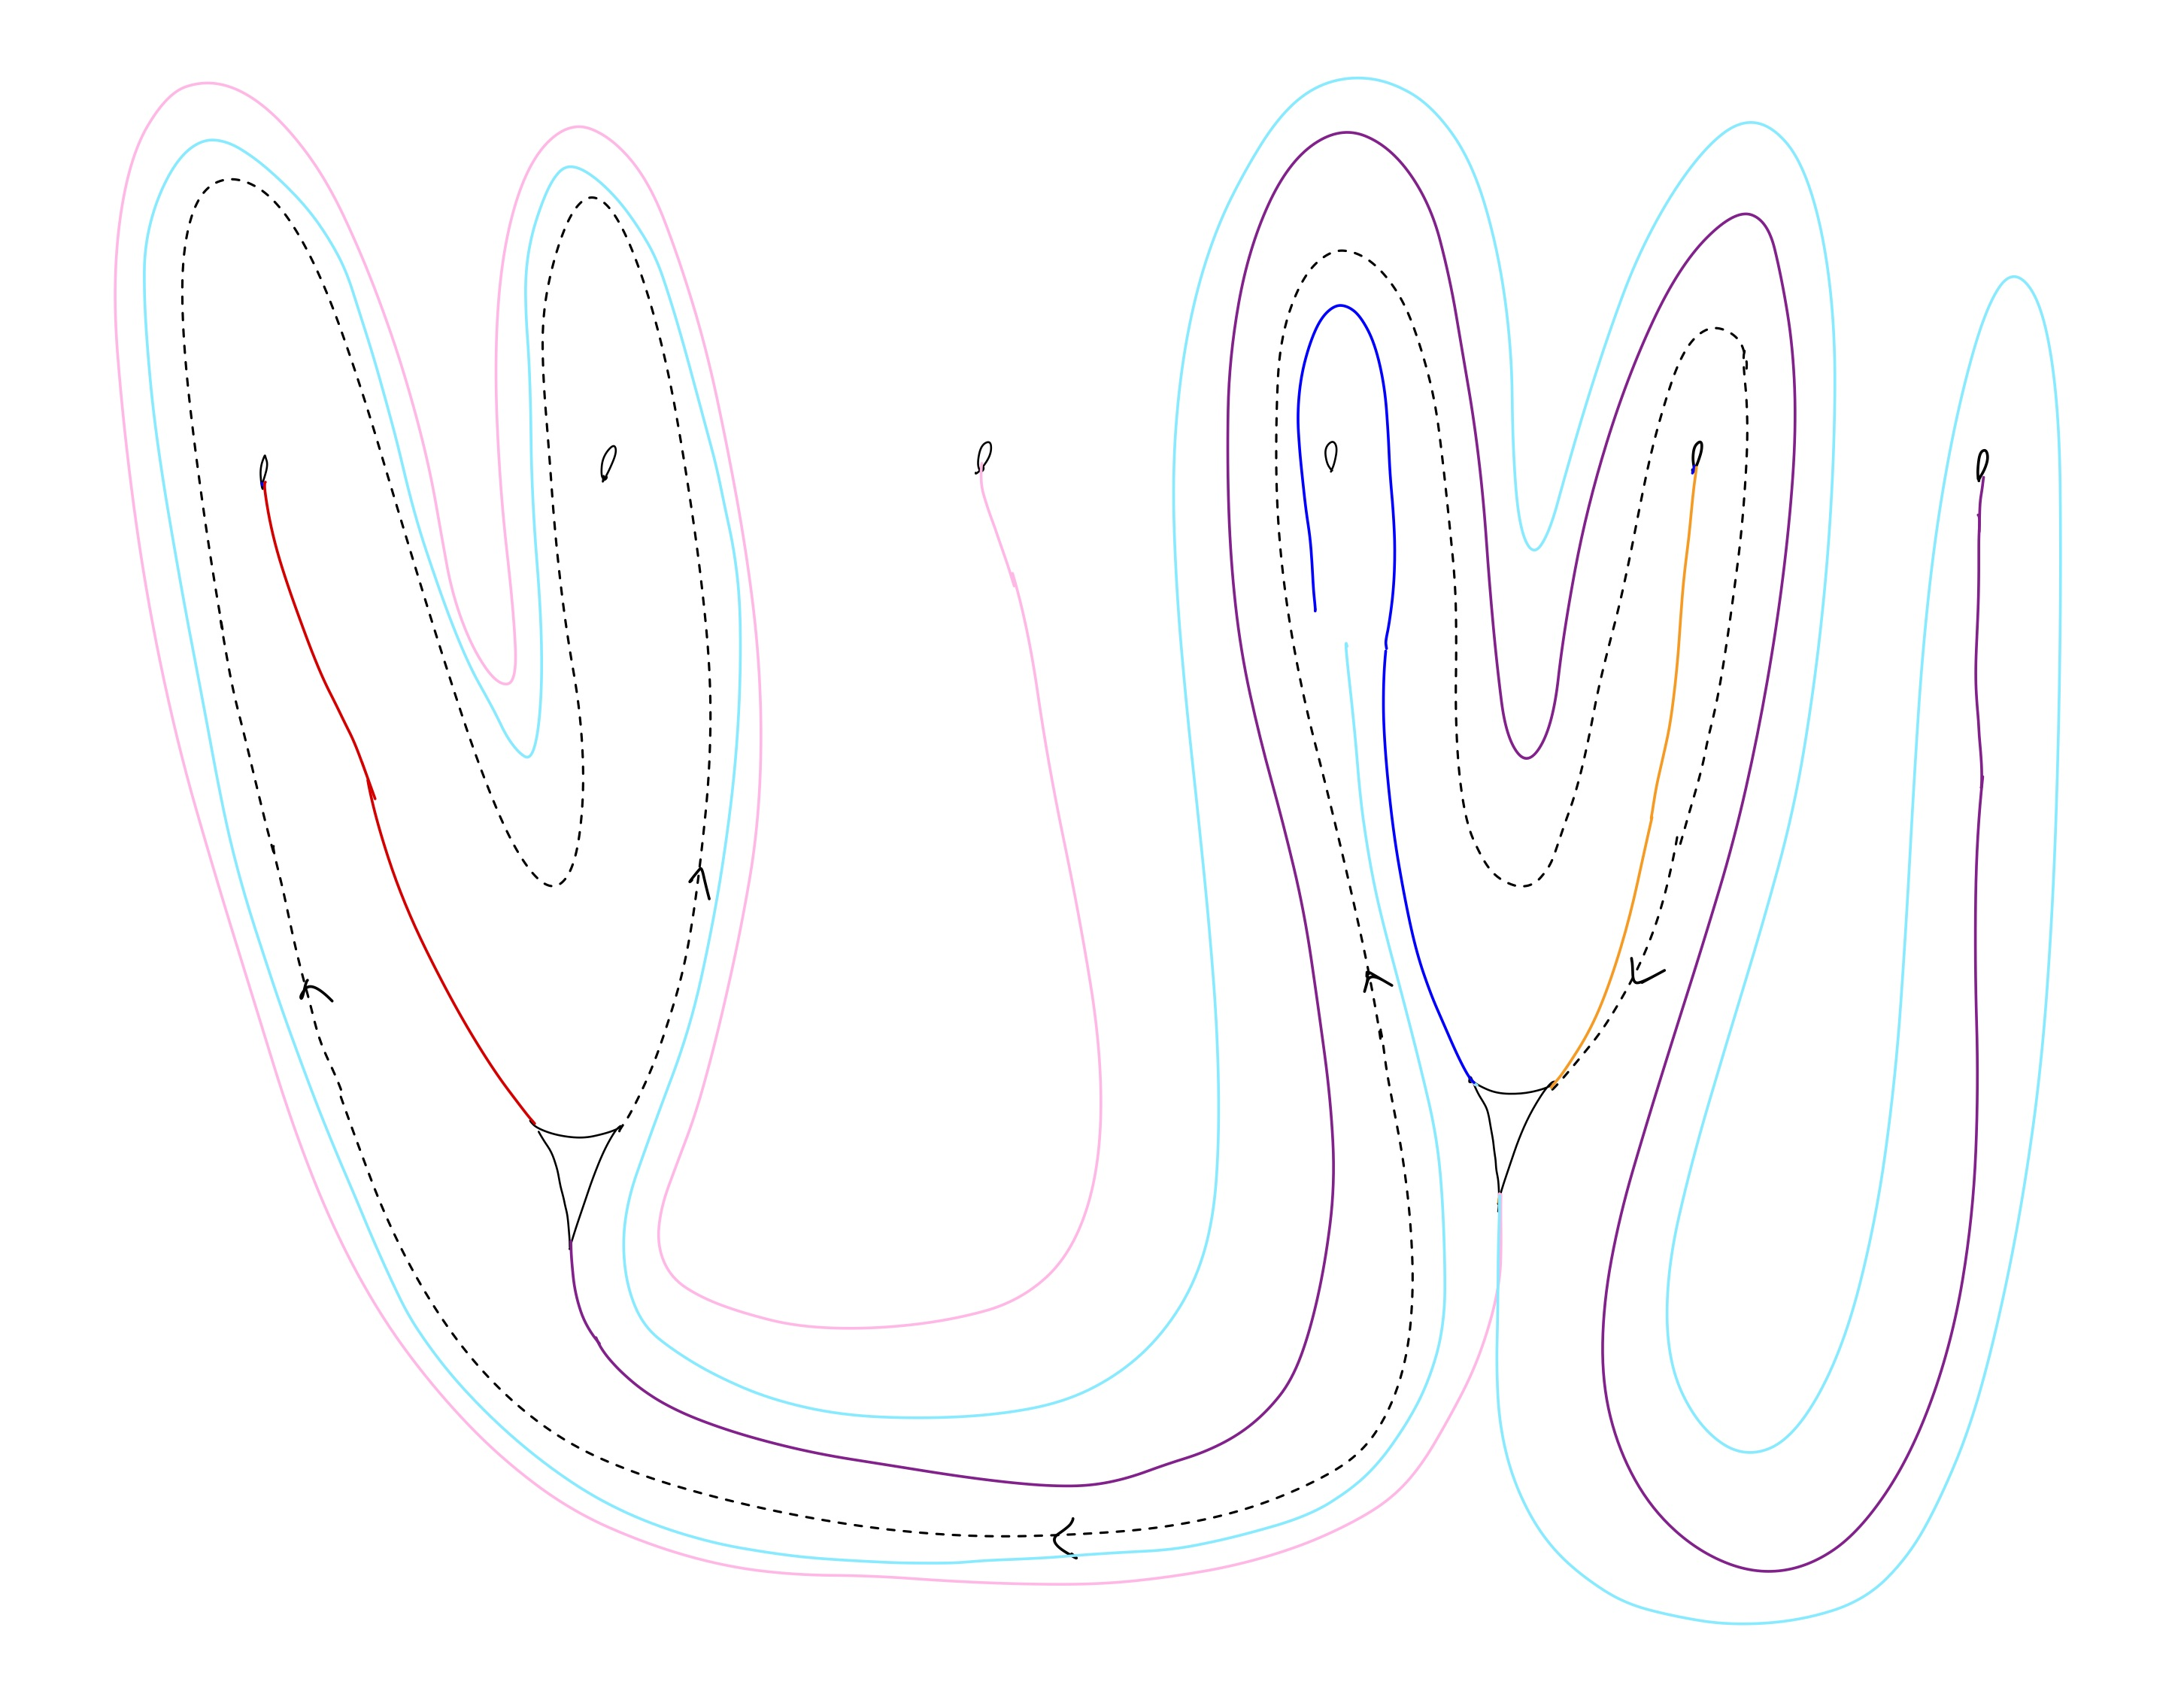
\includegraphics[width=\linewidth]{figures_case_analysis/track17_case_analysis/Blore-4.jpg}
    \caption{Blore4}
    \label{fig:Blore4}
\end{figure}

\begin{figure}[ht]
    \centering
    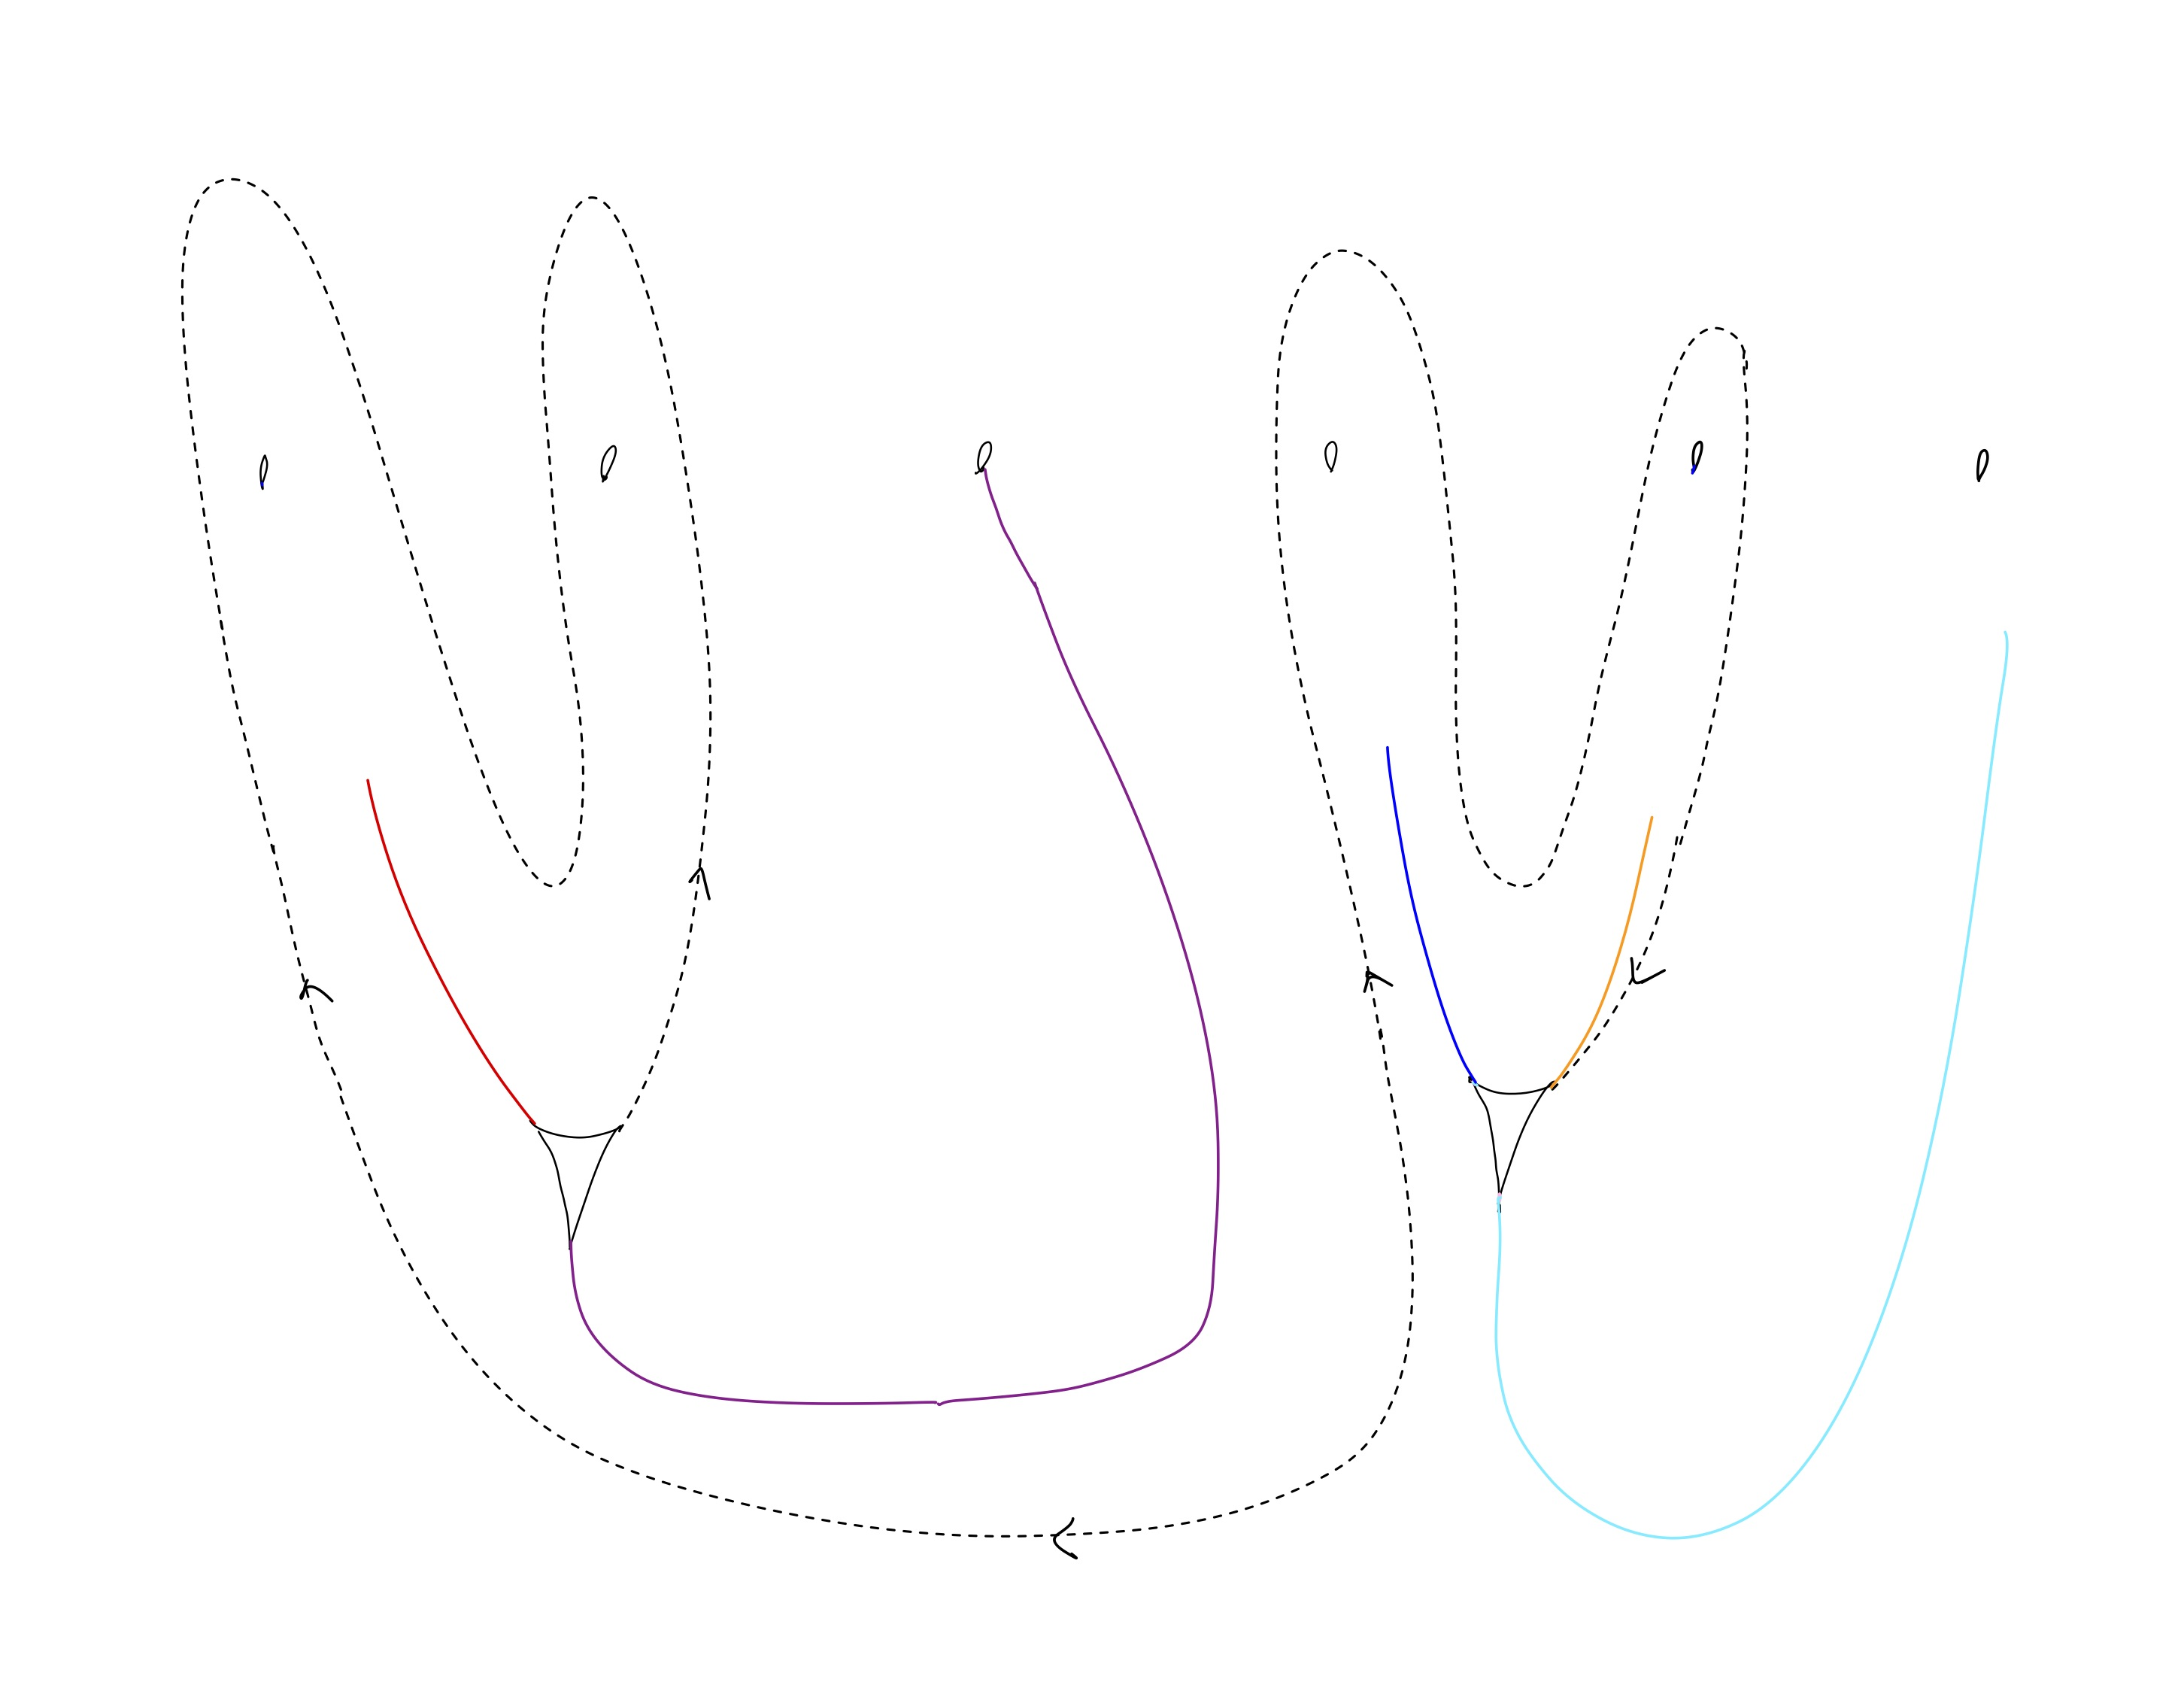
\includegraphics[width=\linewidth]{figures_case_analysis/track17_case_analysis/Chark-1.jpg}
    \caption{Chark1}
    \label{fig:Chark1}
\end{figure}

\begin{figure}[ht]
    \centering
    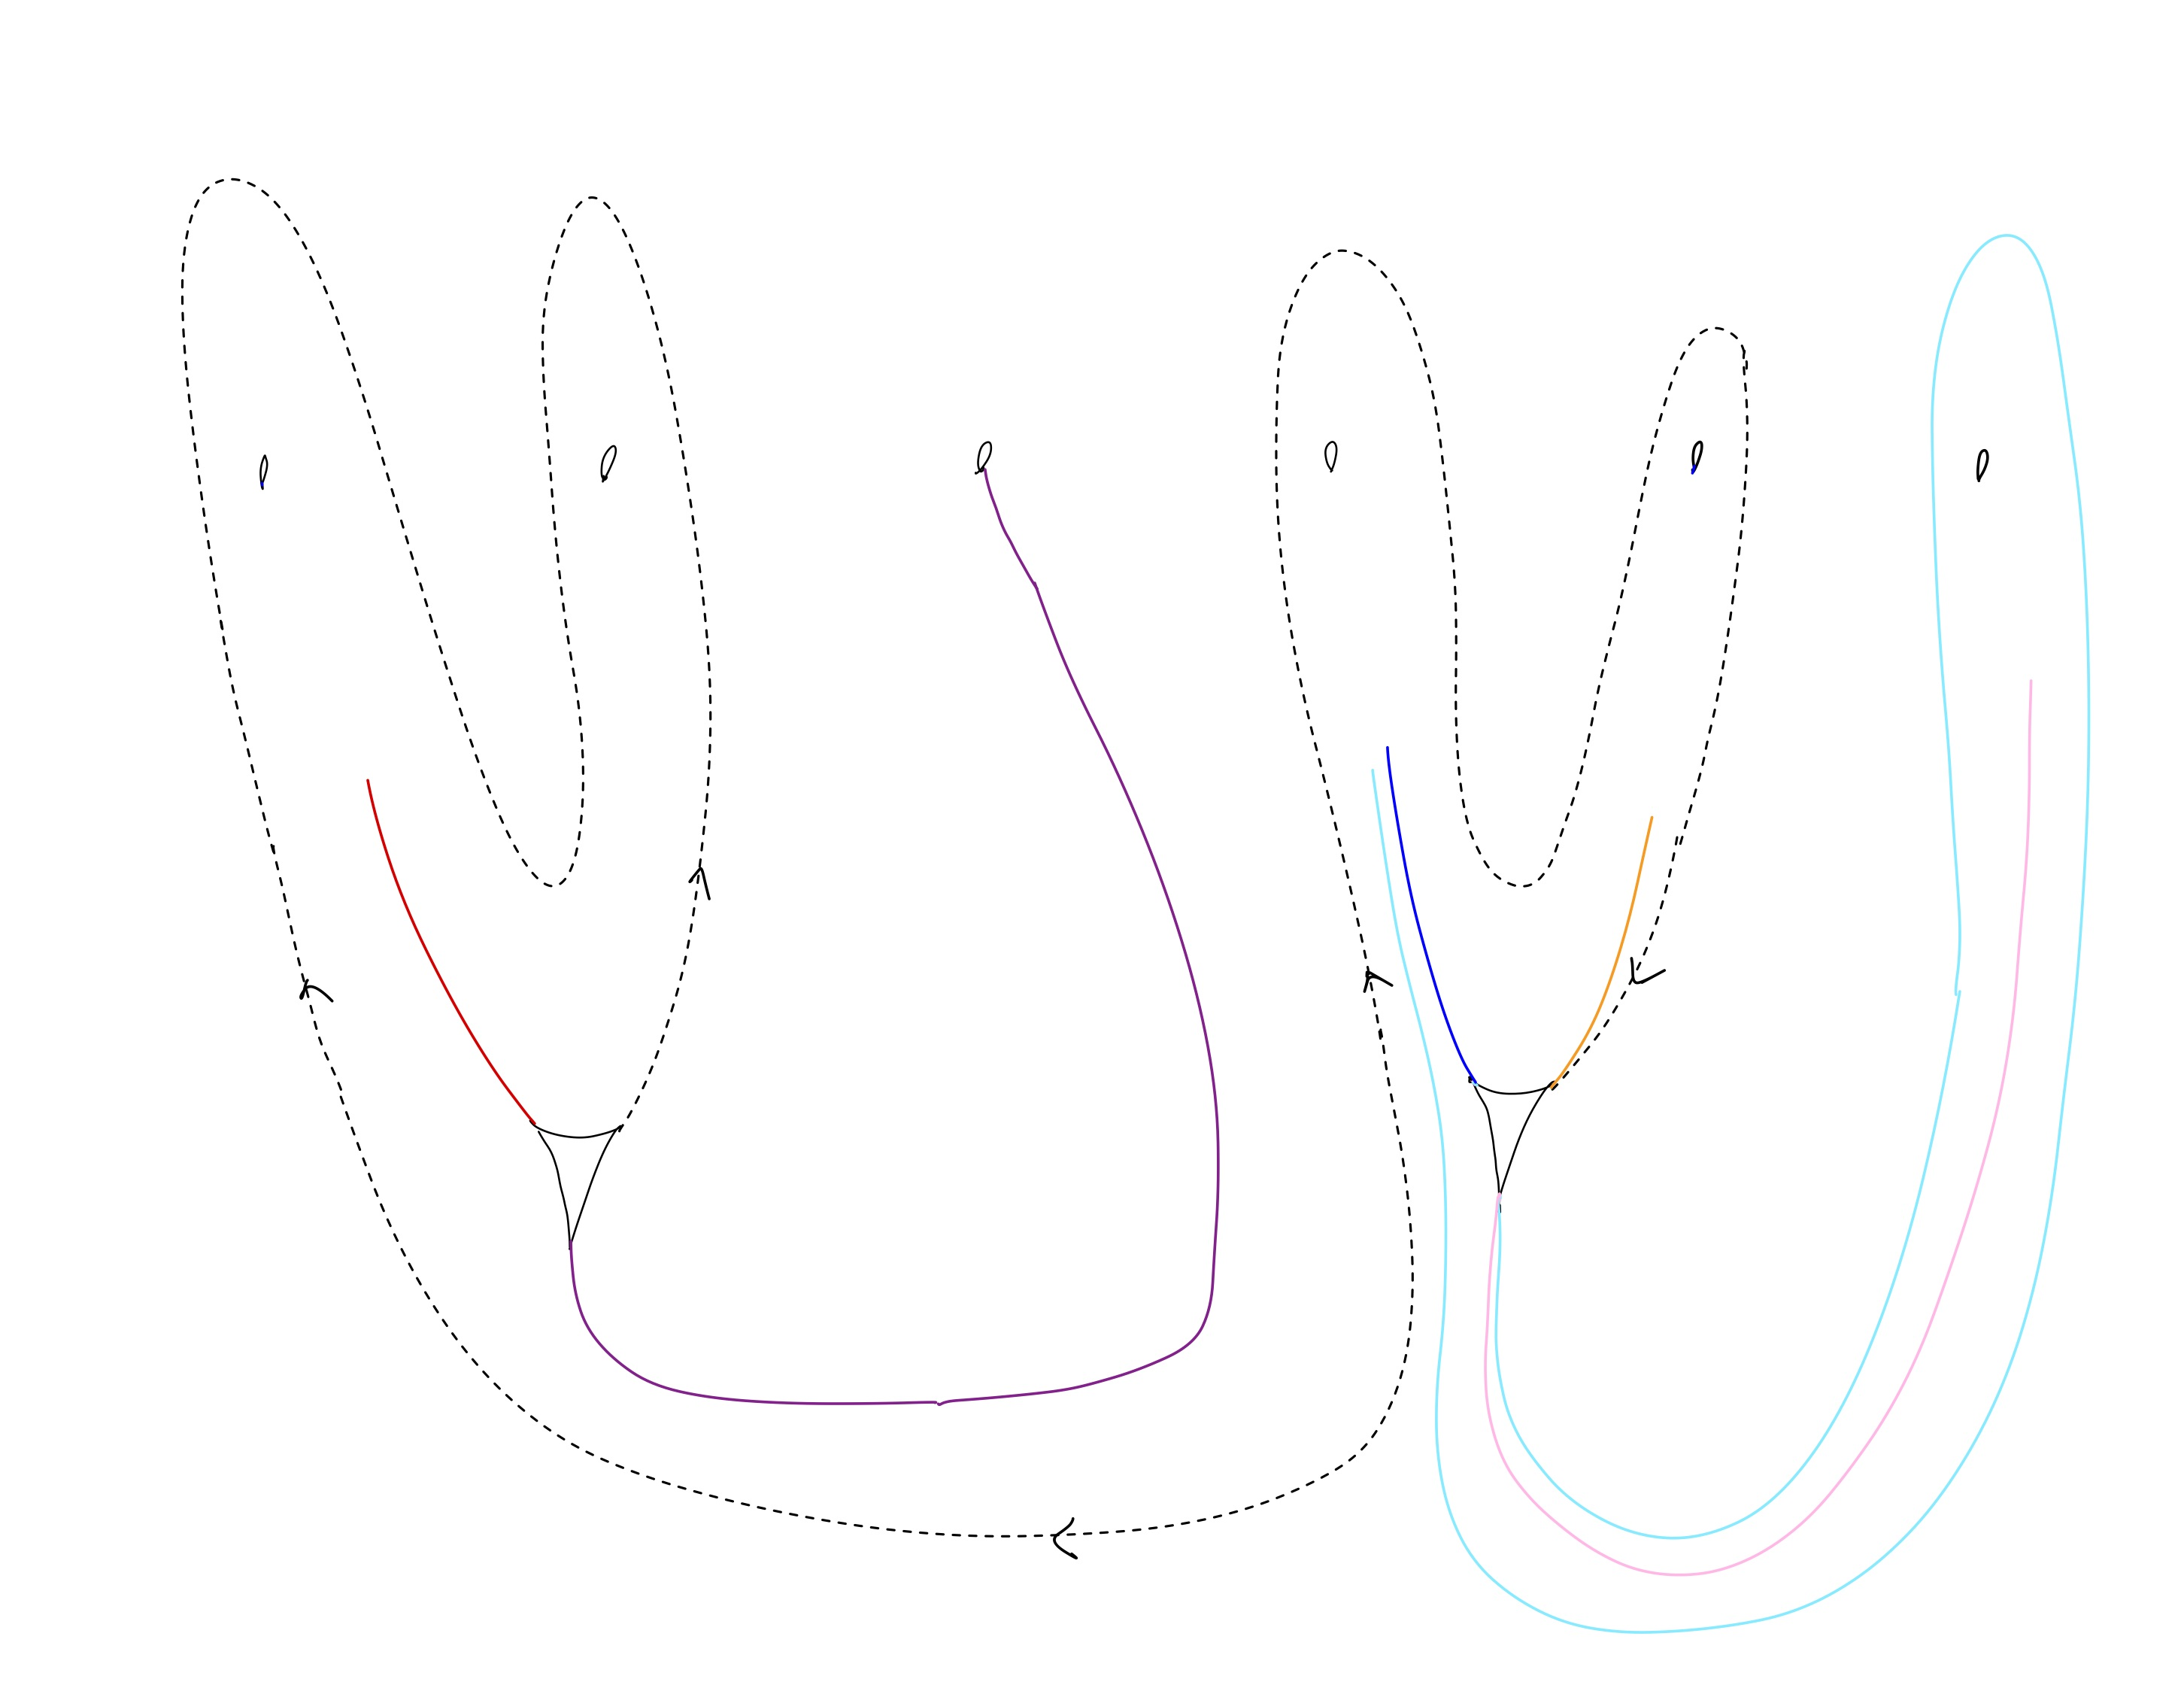
\includegraphics[width=\linewidth]{figures_case_analysis/track17_case_analysis/Chark-2.jpg}
    \caption{Chark2}
    \label{fig:Chark2}
\end{figure}
\clearpage

\begin{figure}[ht]
    \centering
    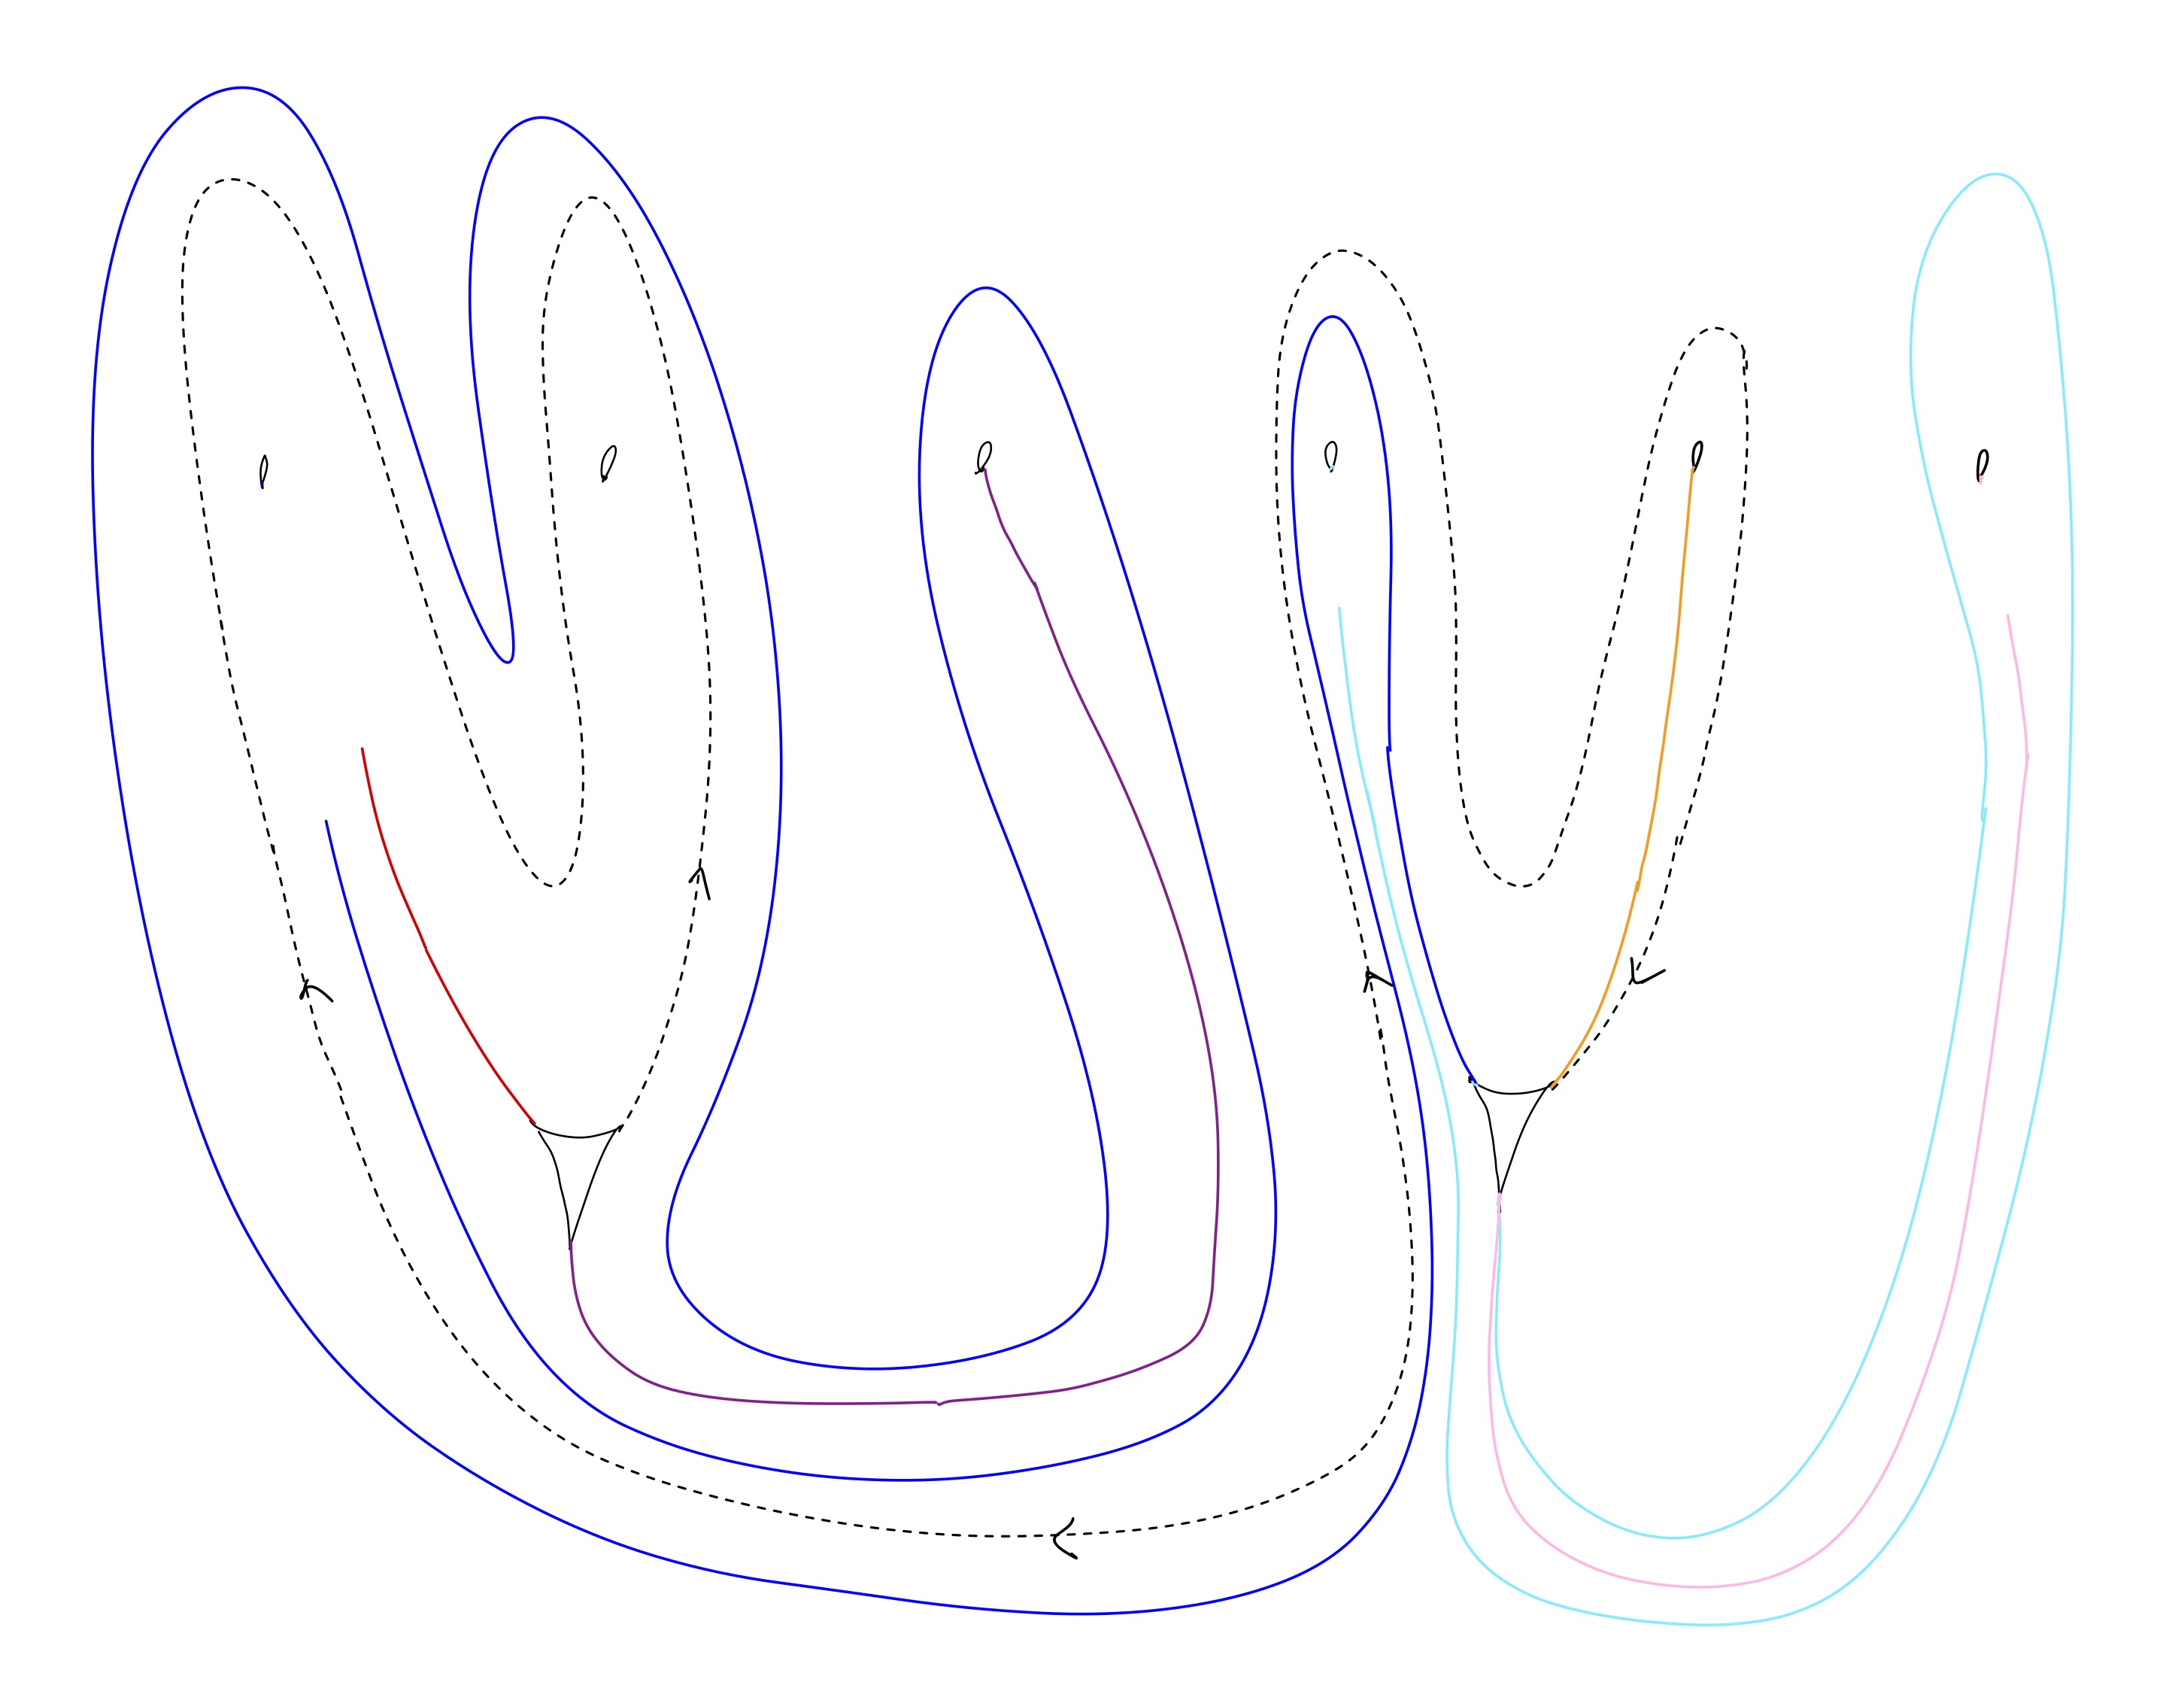
\includegraphics[width=\linewidth]{figures_case_analysis/track17_case_analysis/Cudden-1.jpg}
    \caption{Cudden1}
    \label{fig:Cudden1}
\end{figure}

\begin{figure}[ht]
    \centering
    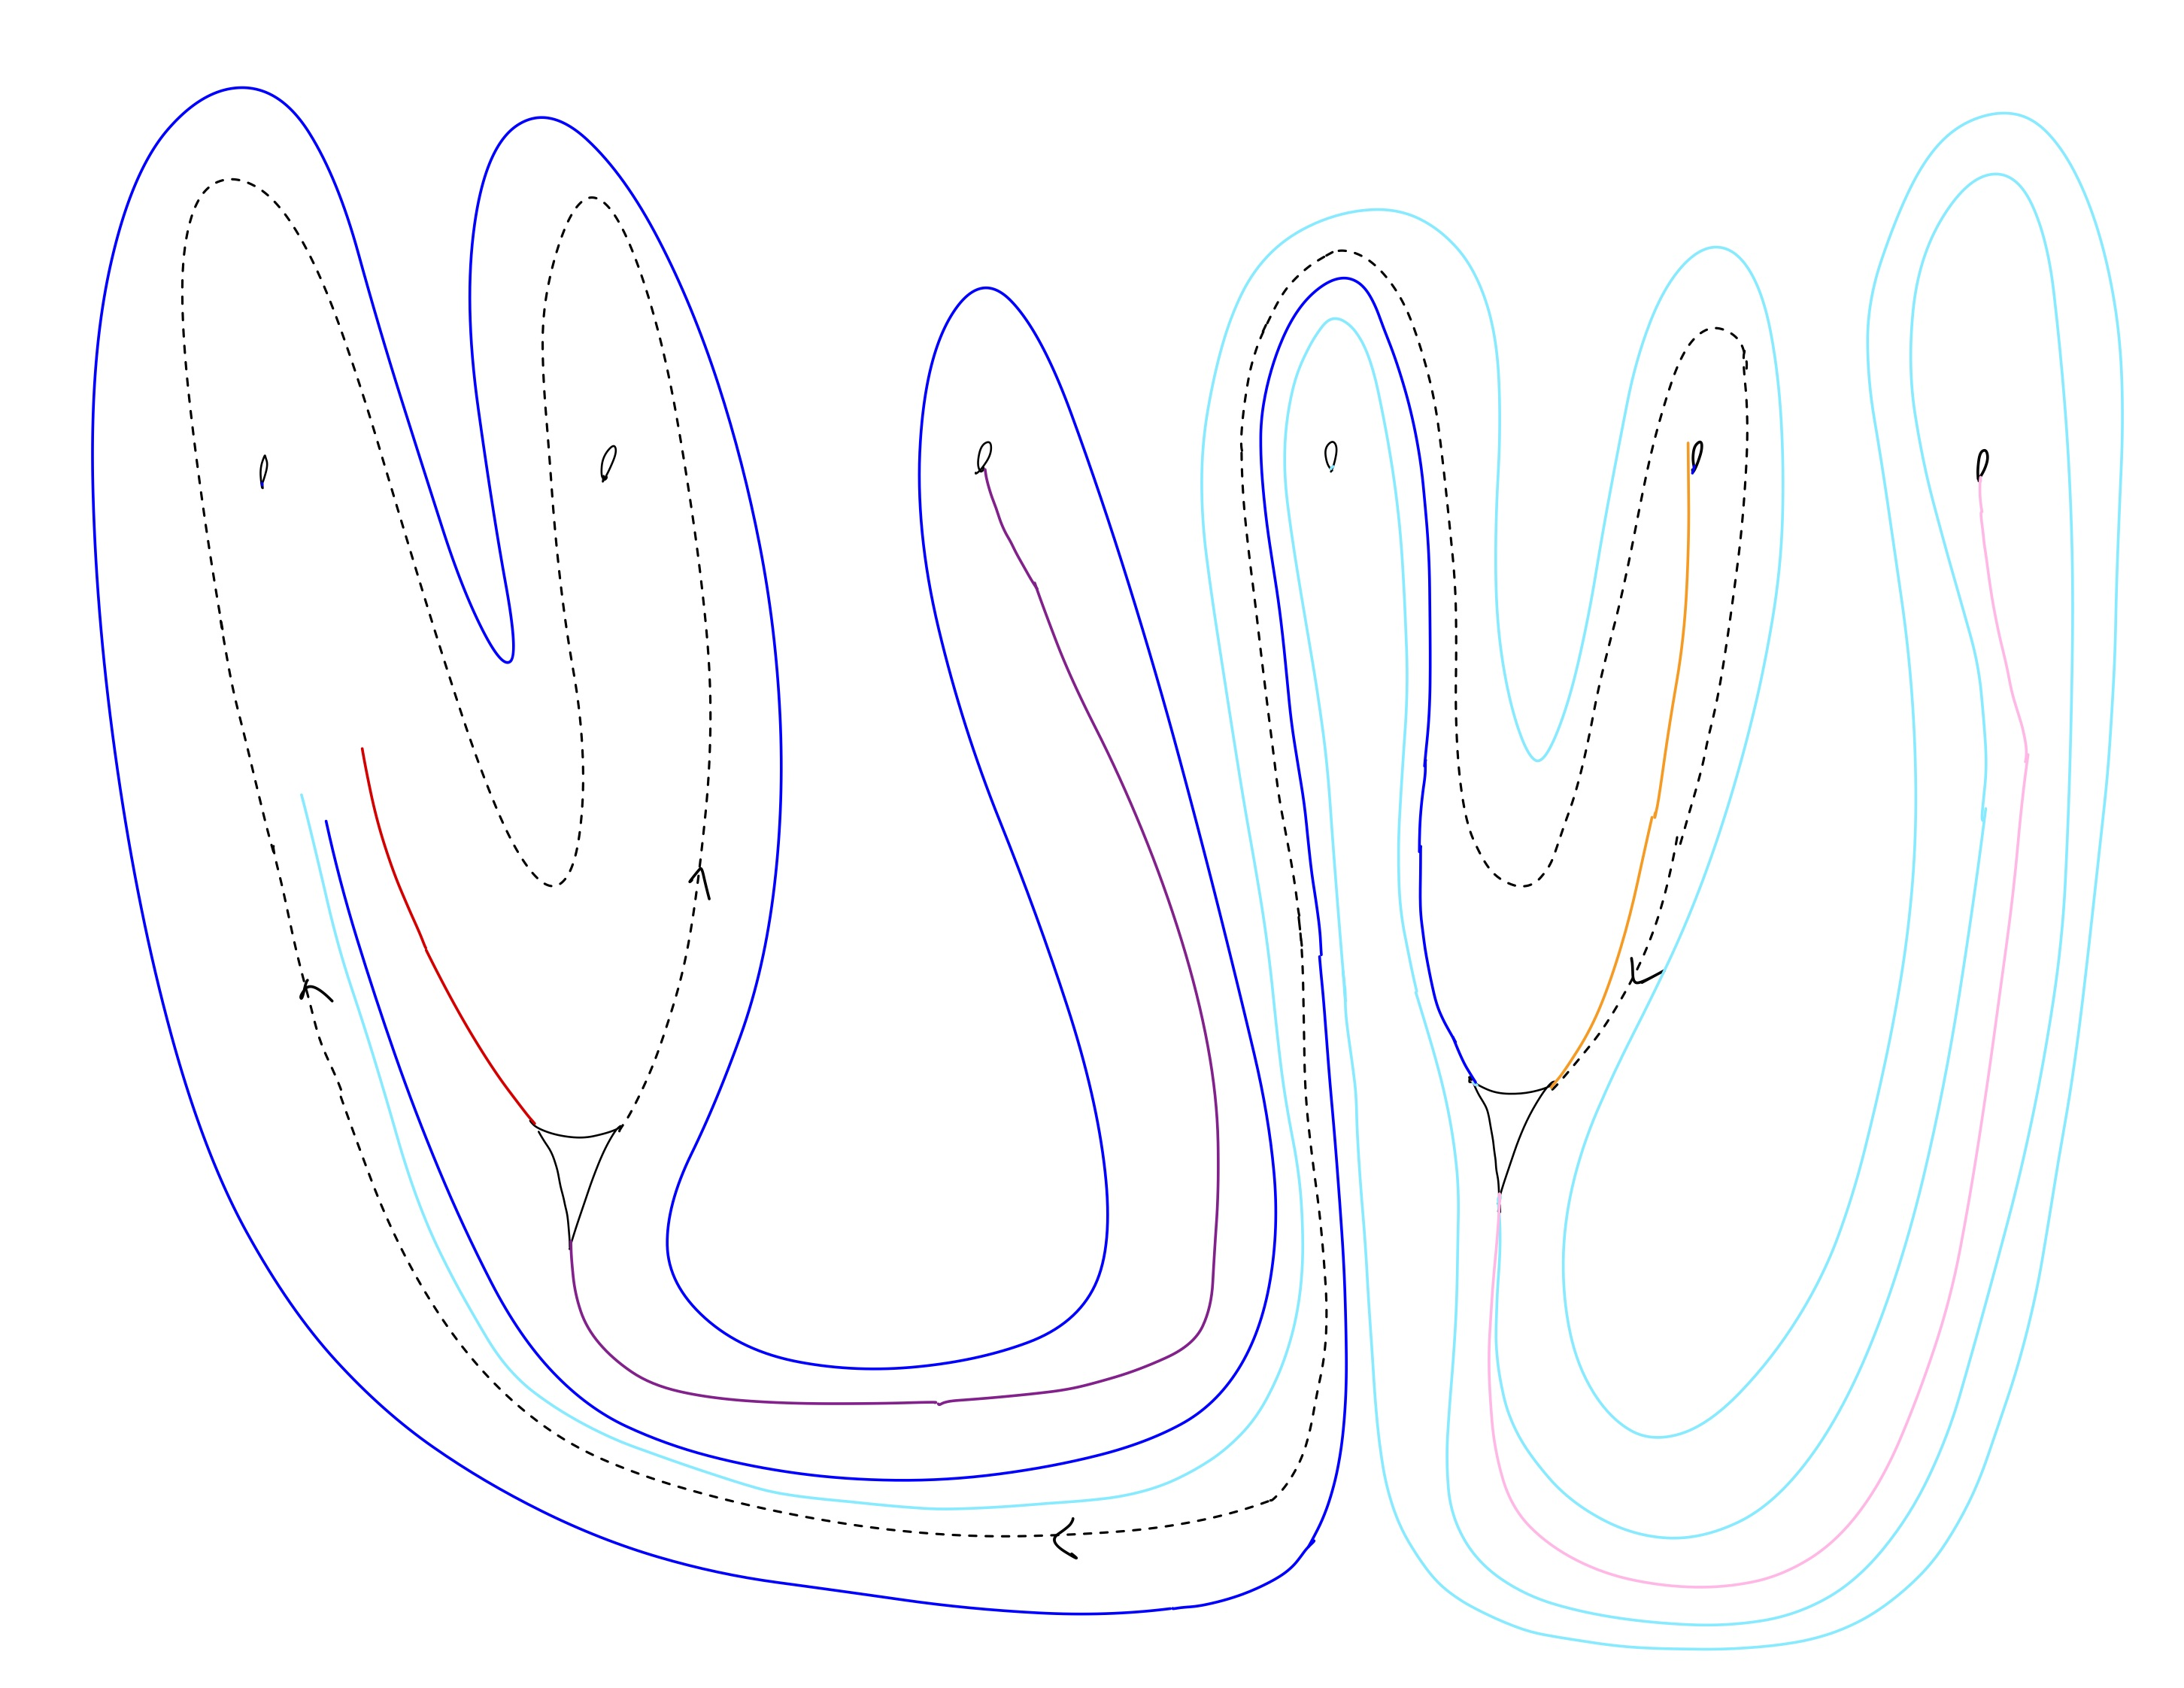
\includegraphics[width=\linewidth]{figures_case_analysis/track17_case_analysis/Cudden-2.jpg}
    \caption{Cudden2}
    \label{fig:Cudden2}
\end{figure}

\begin{figure}[ht]
    \centering
    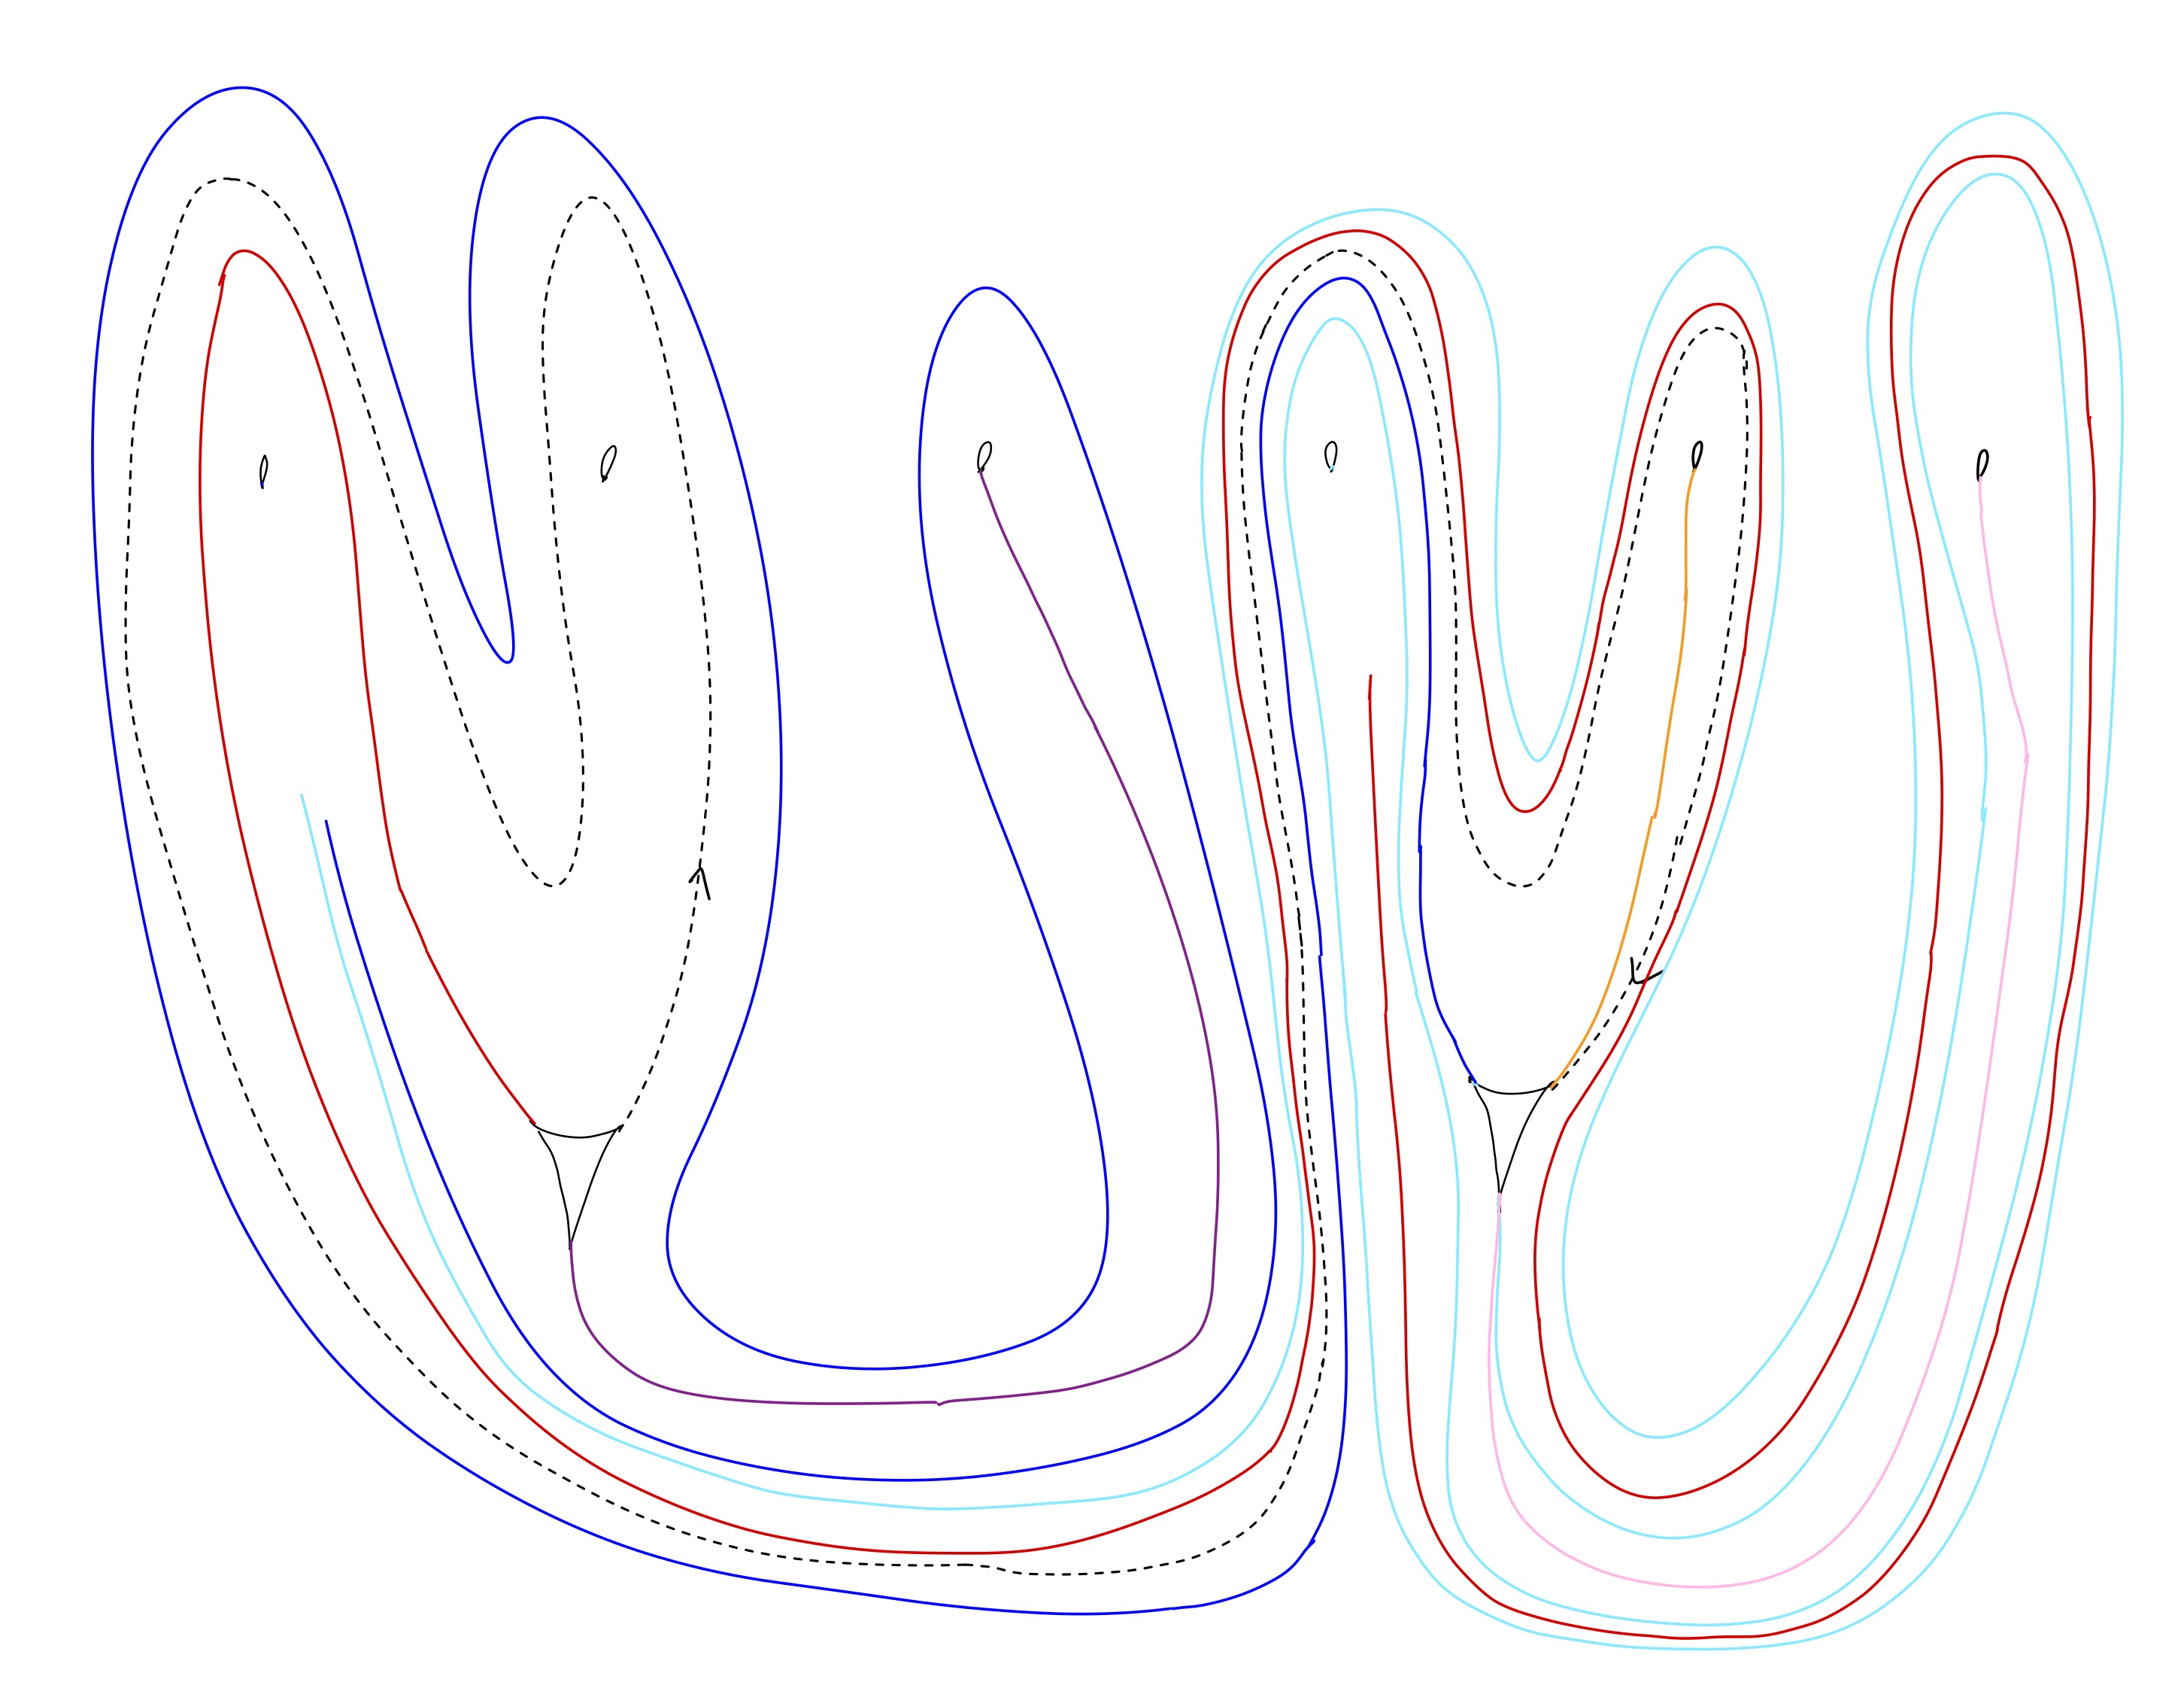
\includegraphics[width=\linewidth]{figures_case_analysis/track17_case_analysis/Cudden-3.jpg}
    \caption{Cudden3}
    \label{fig:Cudden3}
\end{figure}

\begin{figure}[ht]
    \centering
    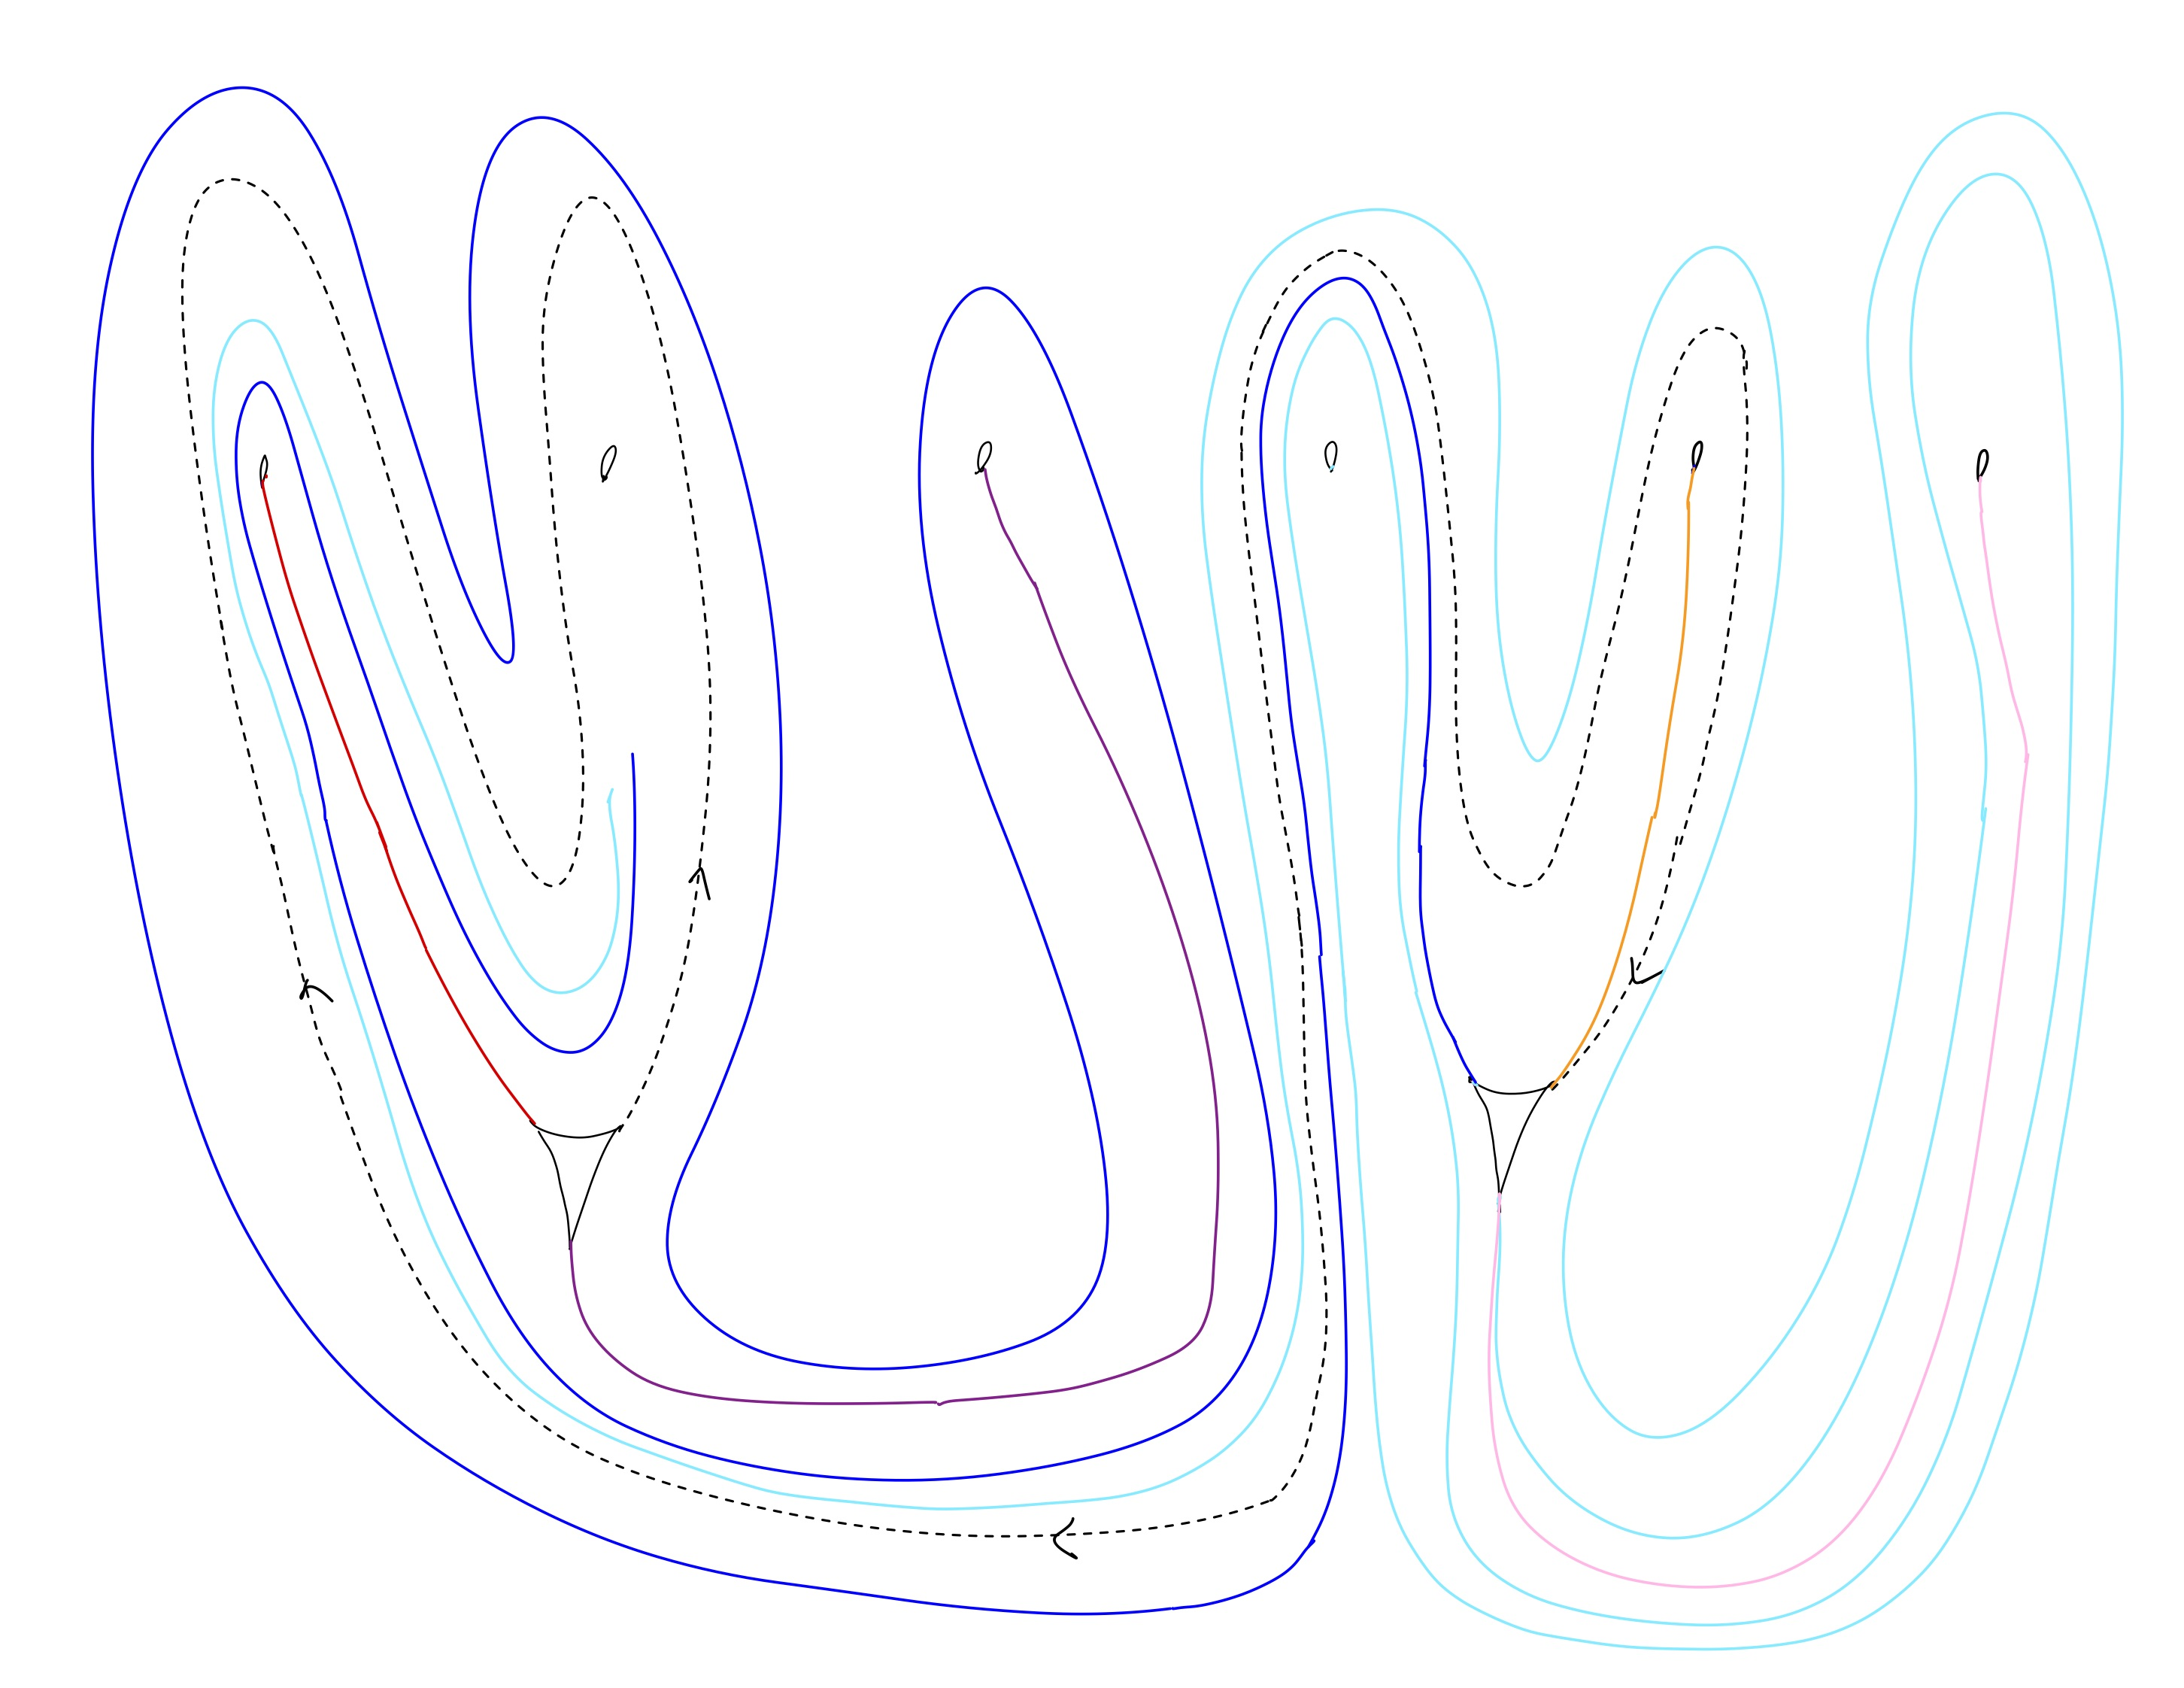
\includegraphics[width=\linewidth]{figures_case_analysis/track17_case_analysis/Cudden-4.jpg}
    \caption{Cudden4}
    \label{fig:Cudden4}
\end{figure}

\begin{figure}[ht]
    \centering
    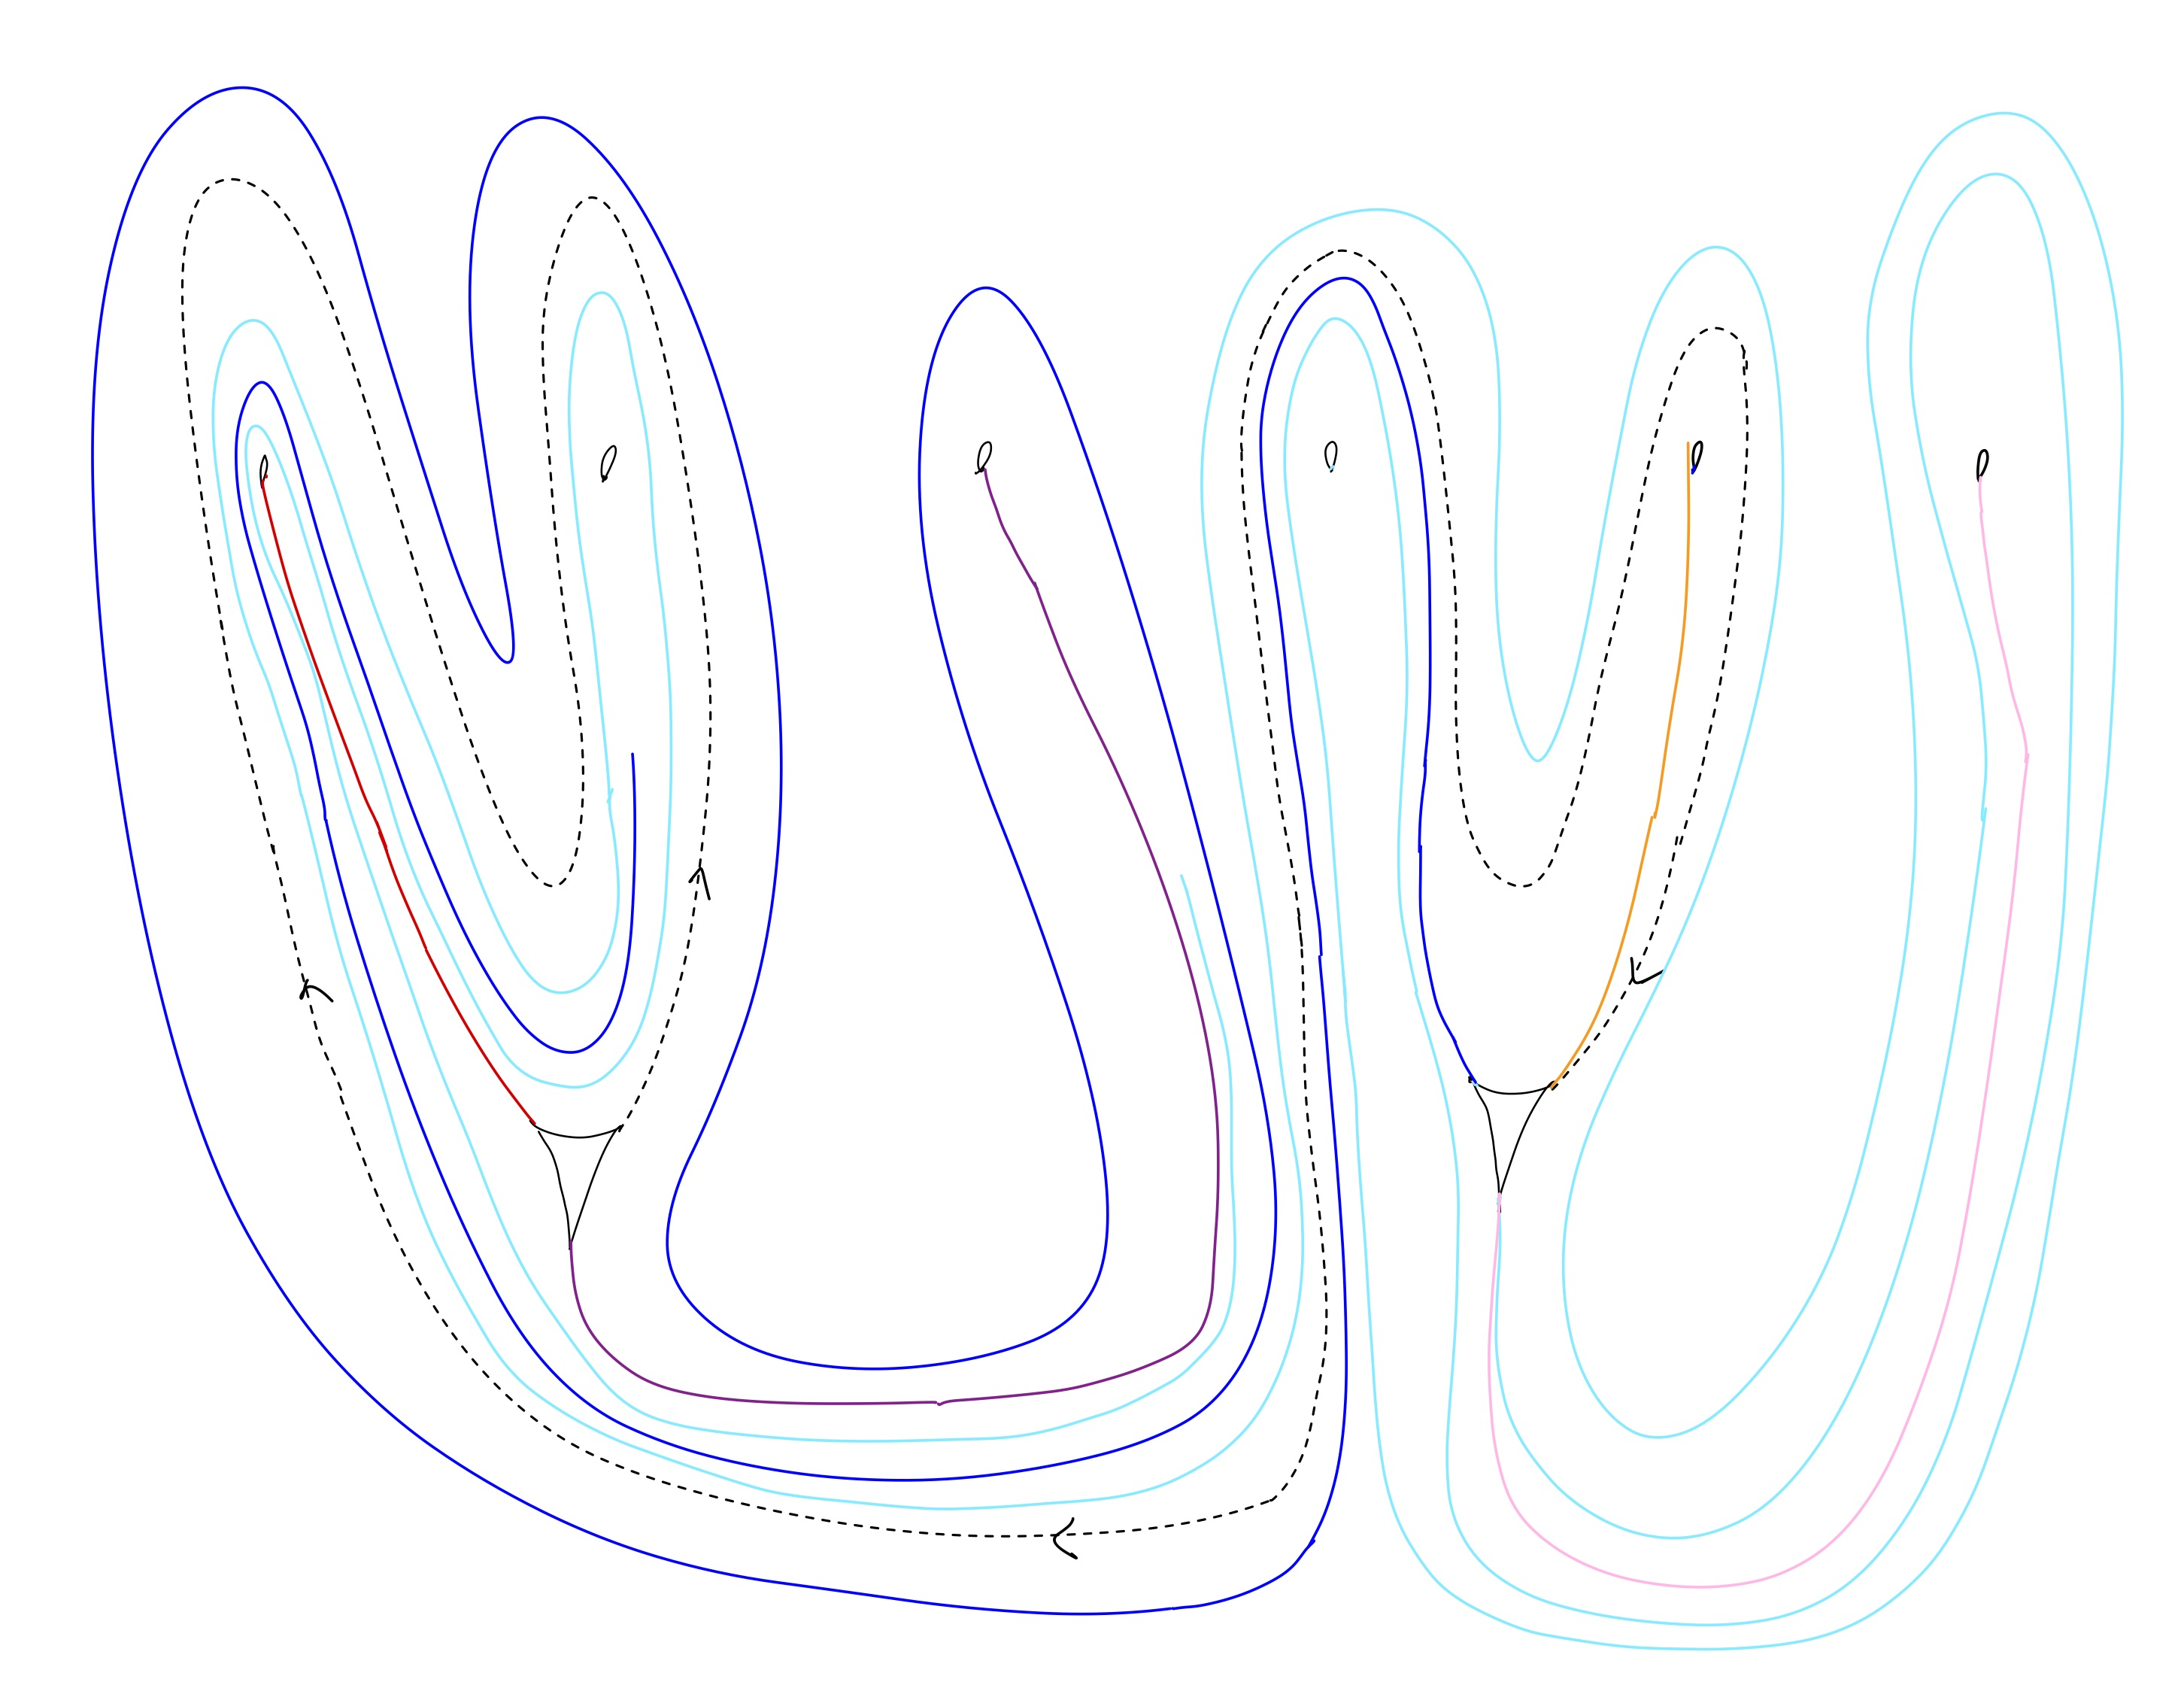
\includegraphics[width=\linewidth]{figures_case_analysis/track17_case_analysis/Cudden-5.jpg}
    \caption{Cudden5}
    \label{fig:Cudden5}
\end{figure}

\begin{figure}[ht]
    \centering
    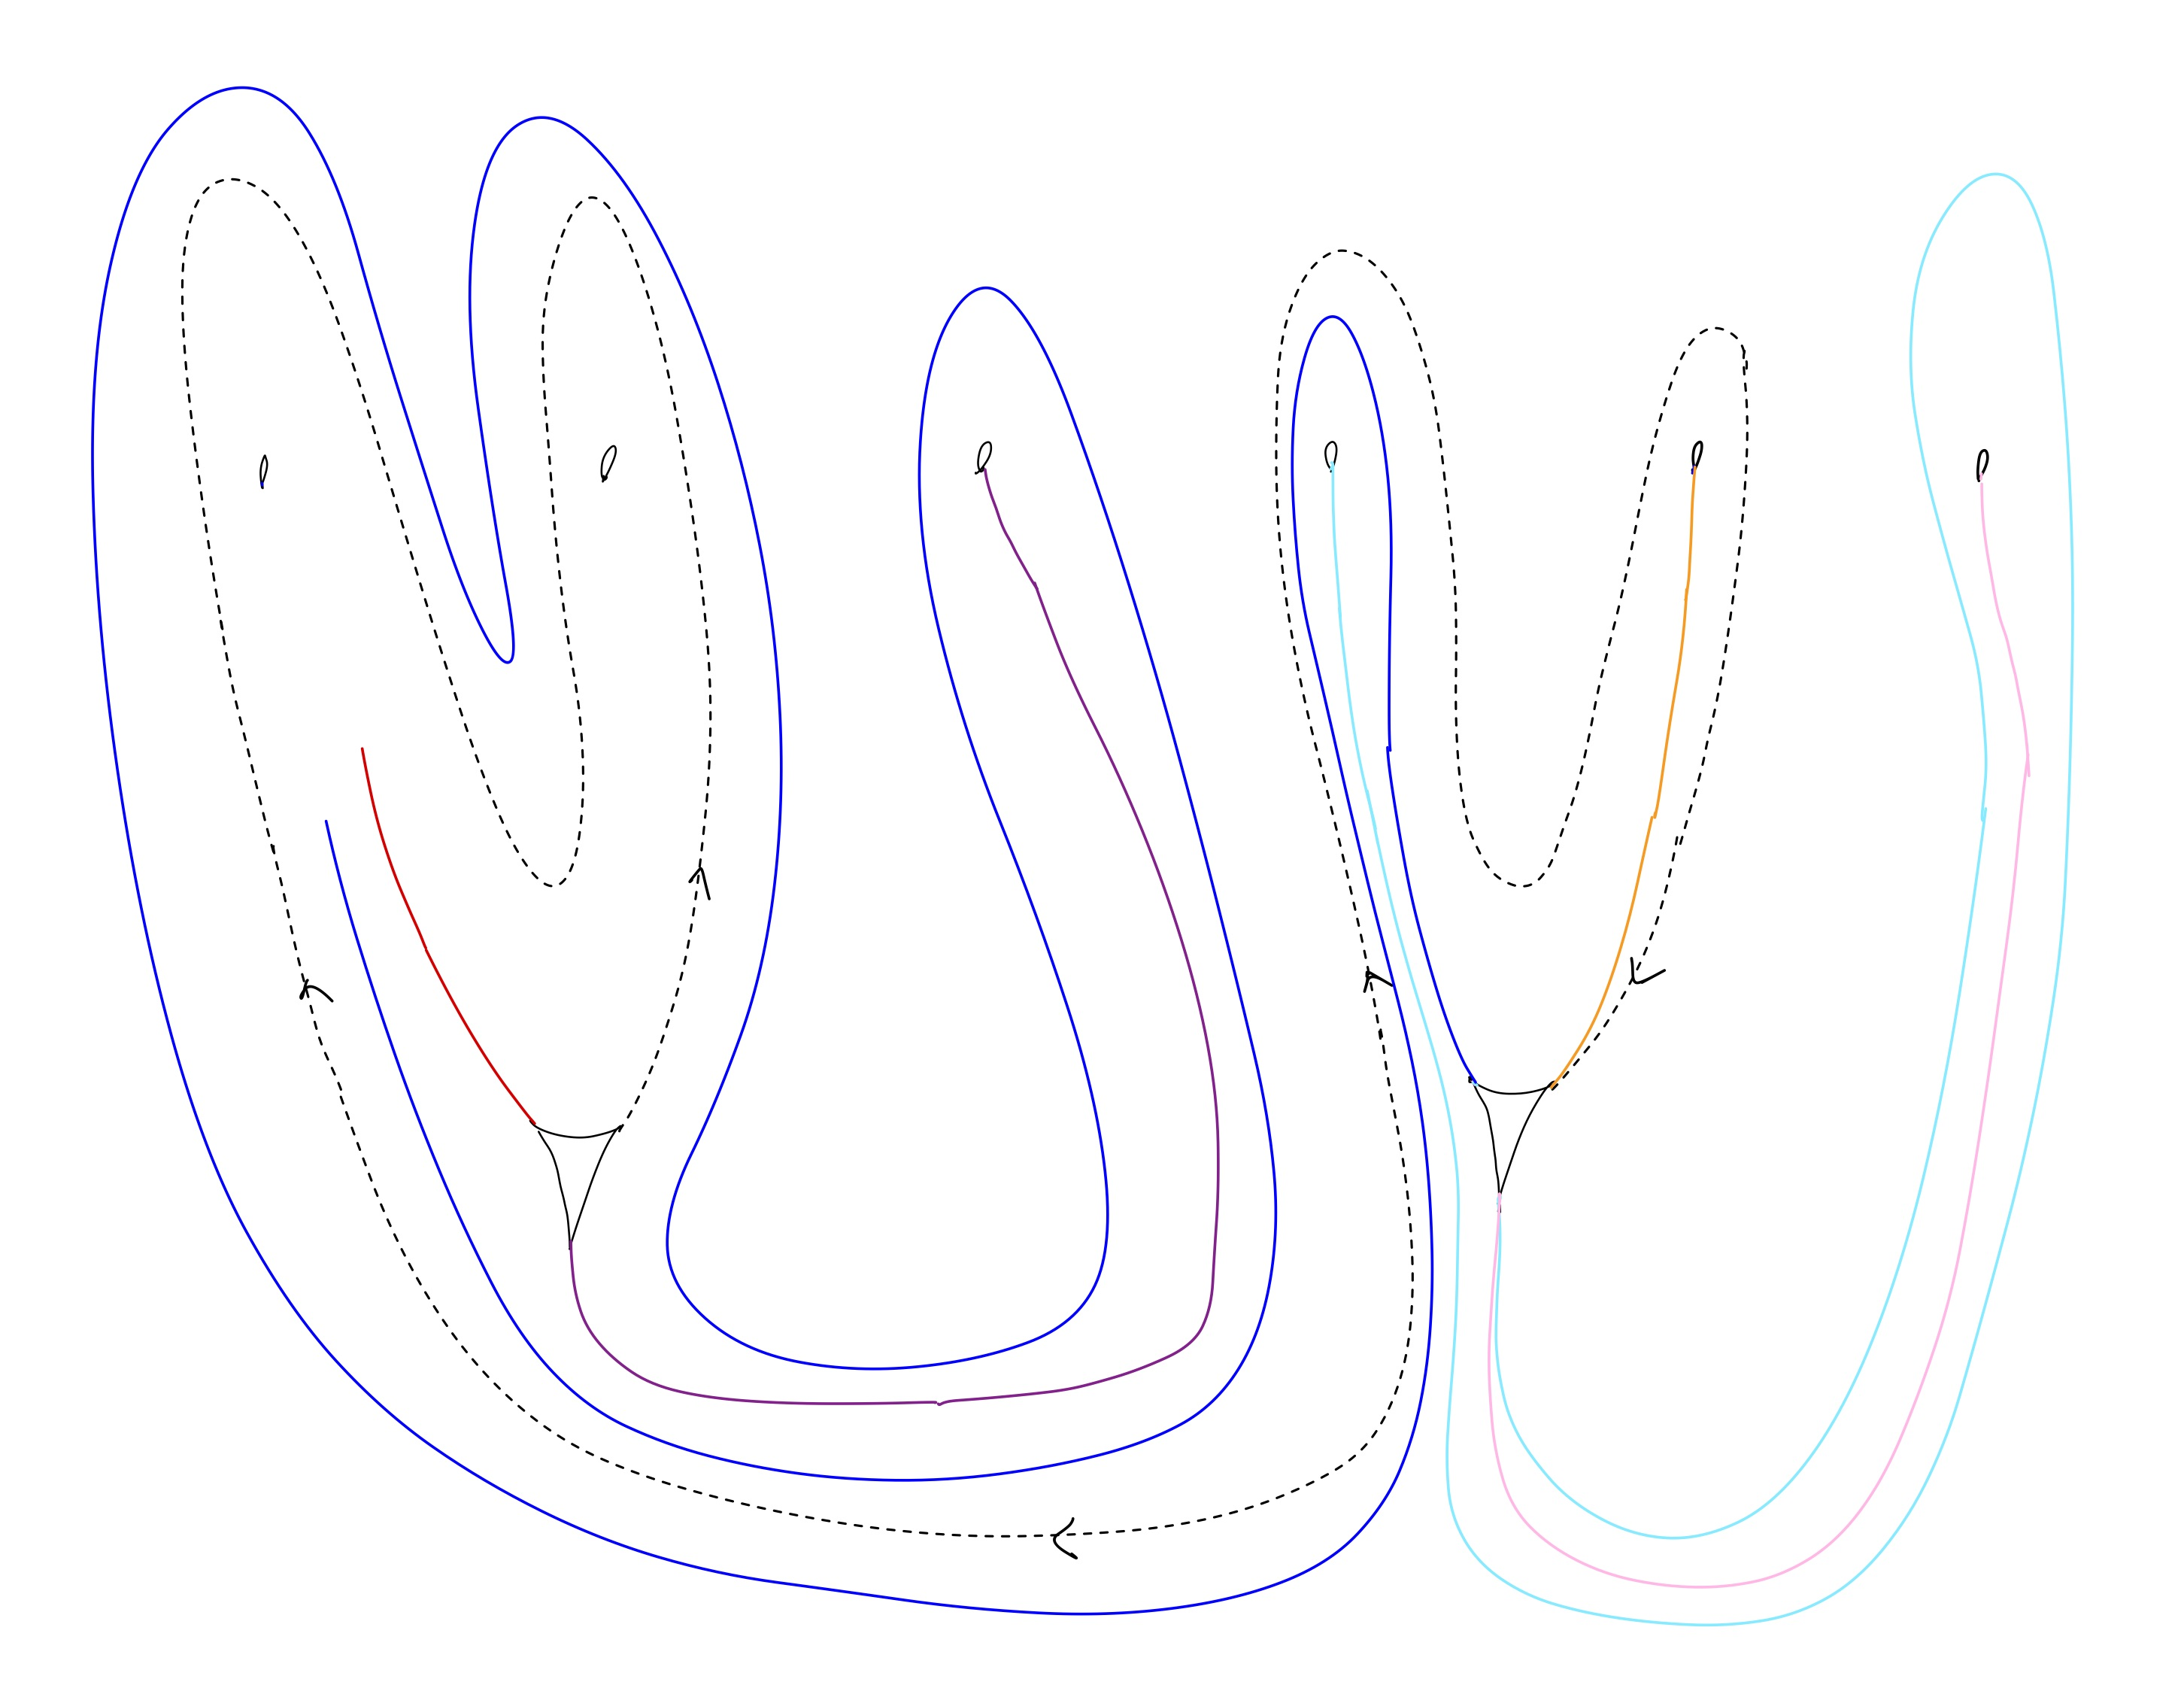
\includegraphics[width=\linewidth]{figures_case_analysis/track17_case_analysis/Cudden-6.jpg}
    \caption{Cudden6}
    \label{fig:Cudden6}
\end{figure}

\begin{figure}[ht]
    \centering
    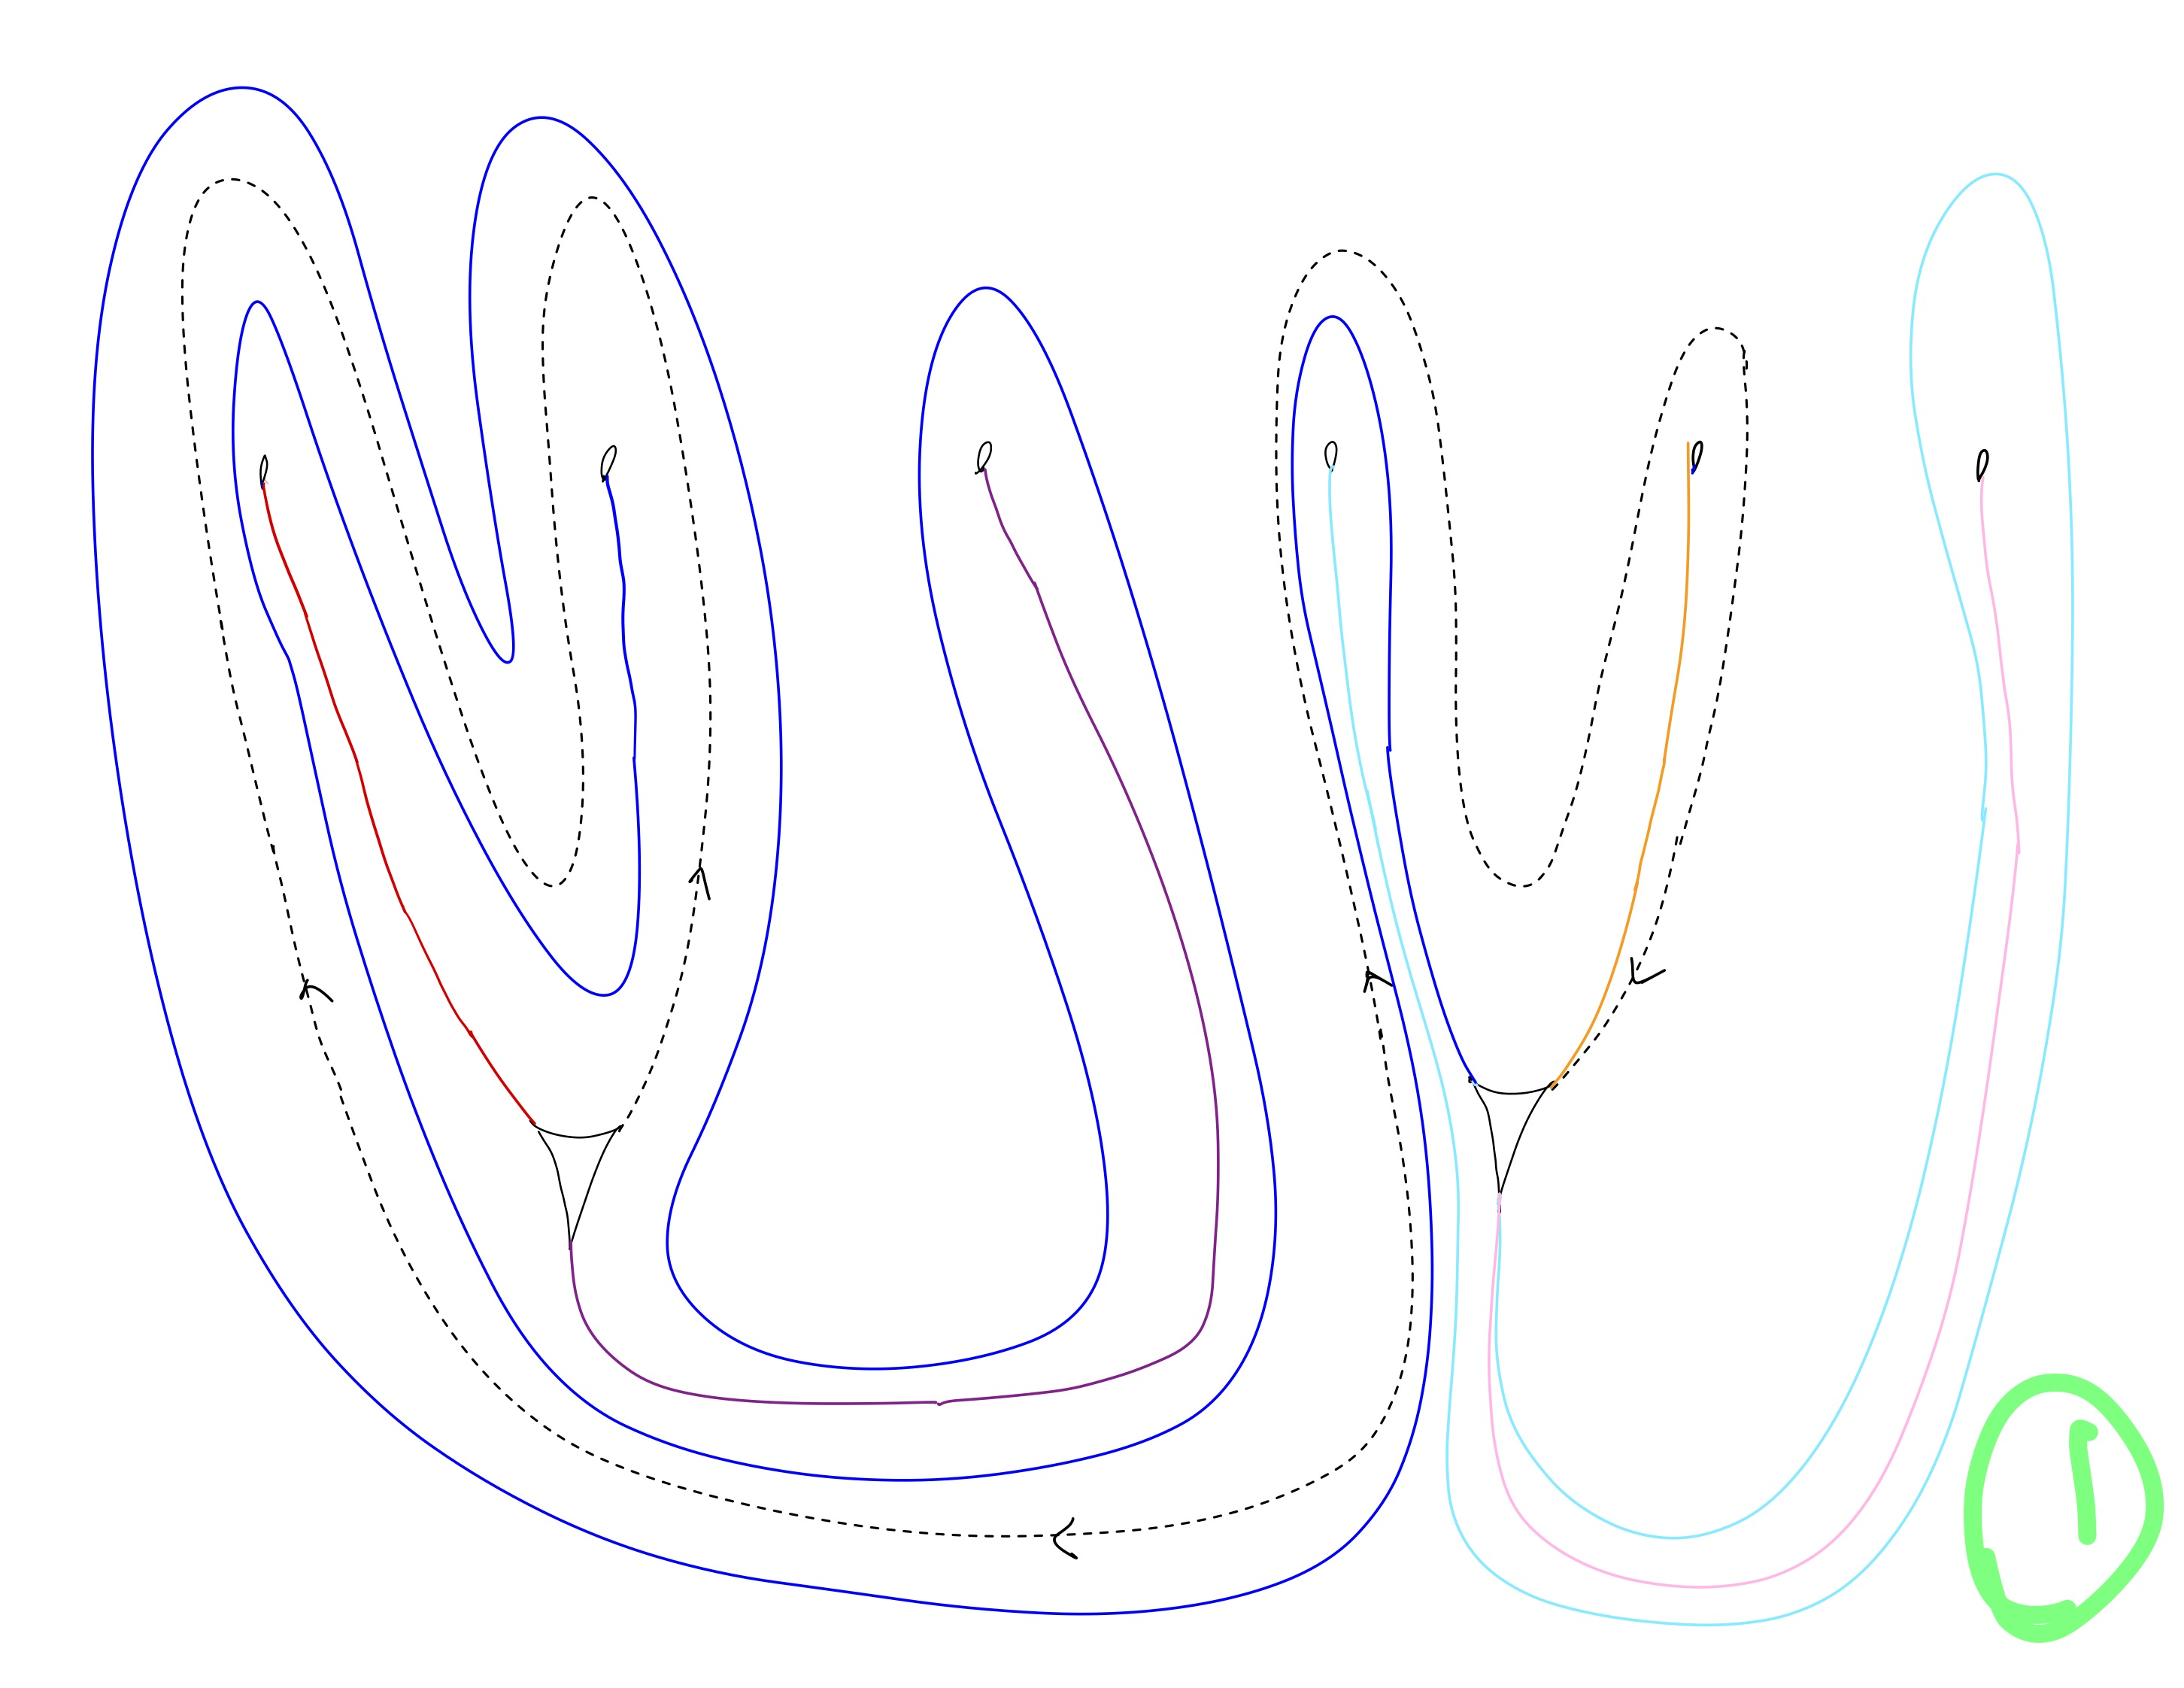
\includegraphics[width=\linewidth]{figures_case_analysis/track17_case_analysis/Cudden-7.jpg}
    \caption{Cudden7}
    \label{fig:Cudden7}
\end{figure}

\clearpage

\begin{figure}[ht]
    \centering
    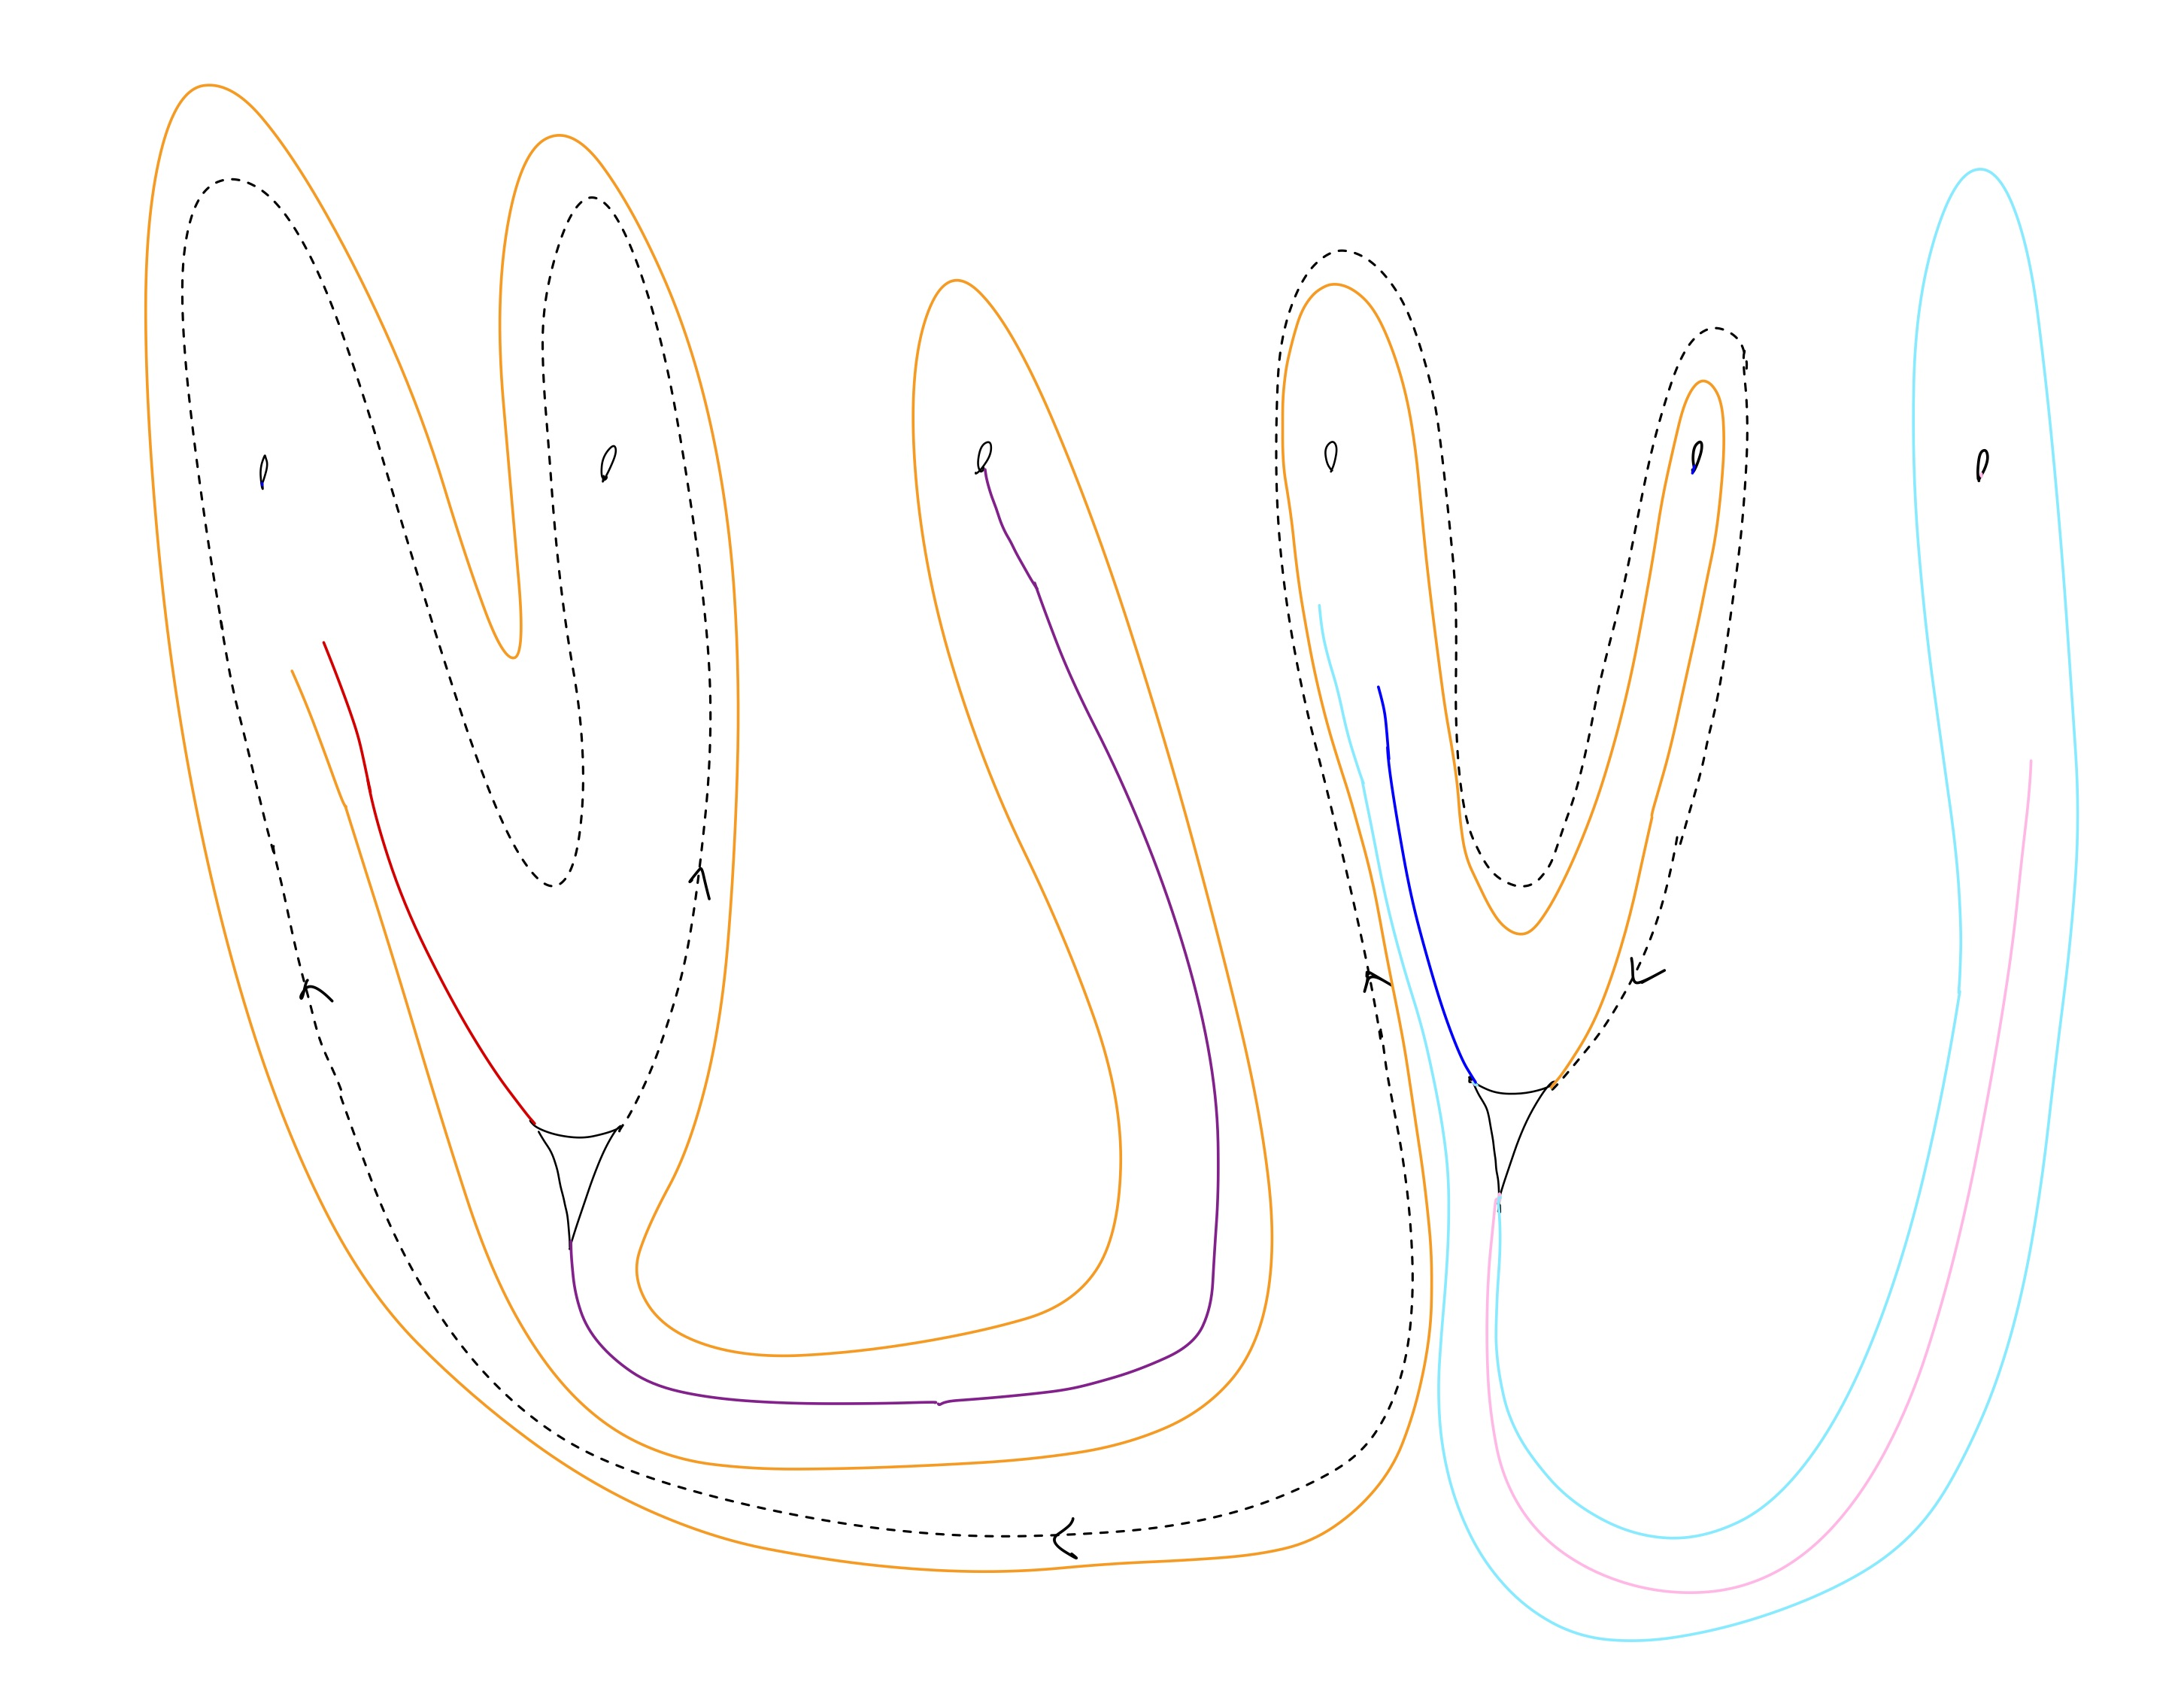
\includegraphics[width=\linewidth]{figures_case_analysis/track17_case_analysis/Flisky-01.jpg}
    \caption{Flisky1}
    \label{fig:Flisky1}
\end{figure}

\begin{figure}[ht]
    \centering
    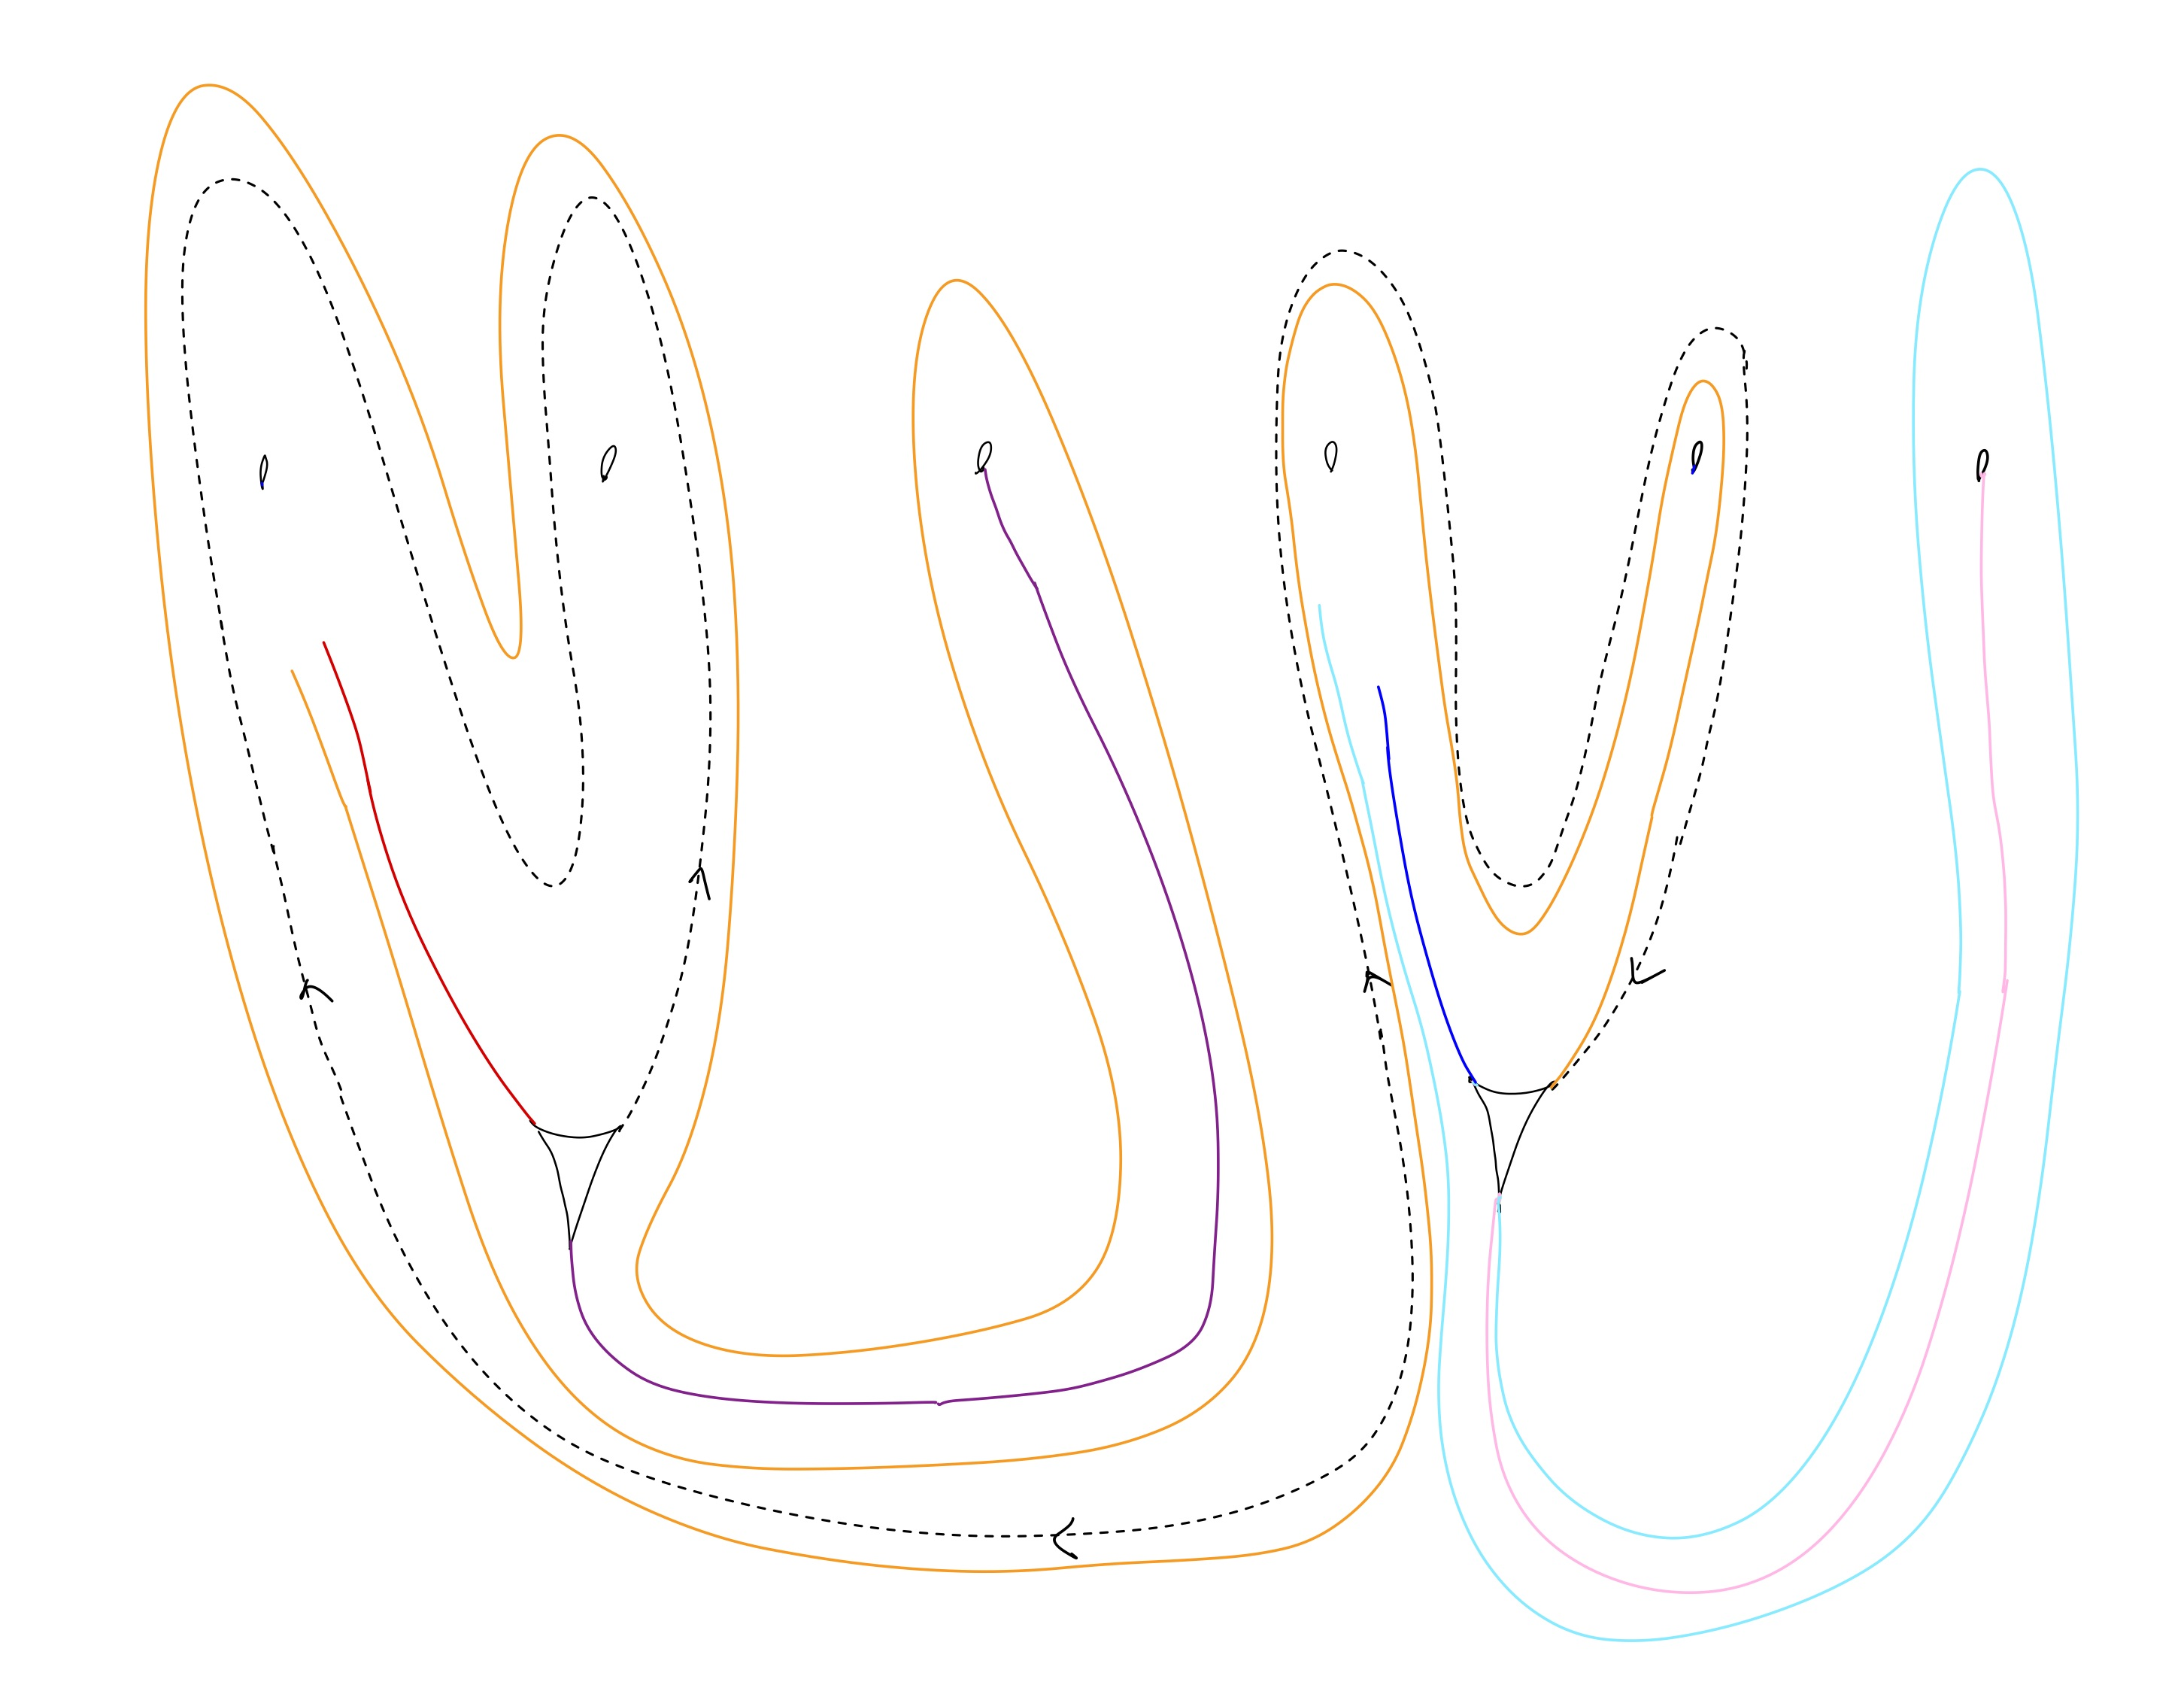
\includegraphics[width=\linewidth]{figures_case_analysis/track17_case_analysis/Flisky-02.jpg}
    \caption{Flisky2}
    \label{fig:Flisky2}
\end{figure}

\begin{figure}[ht]
    \centering
    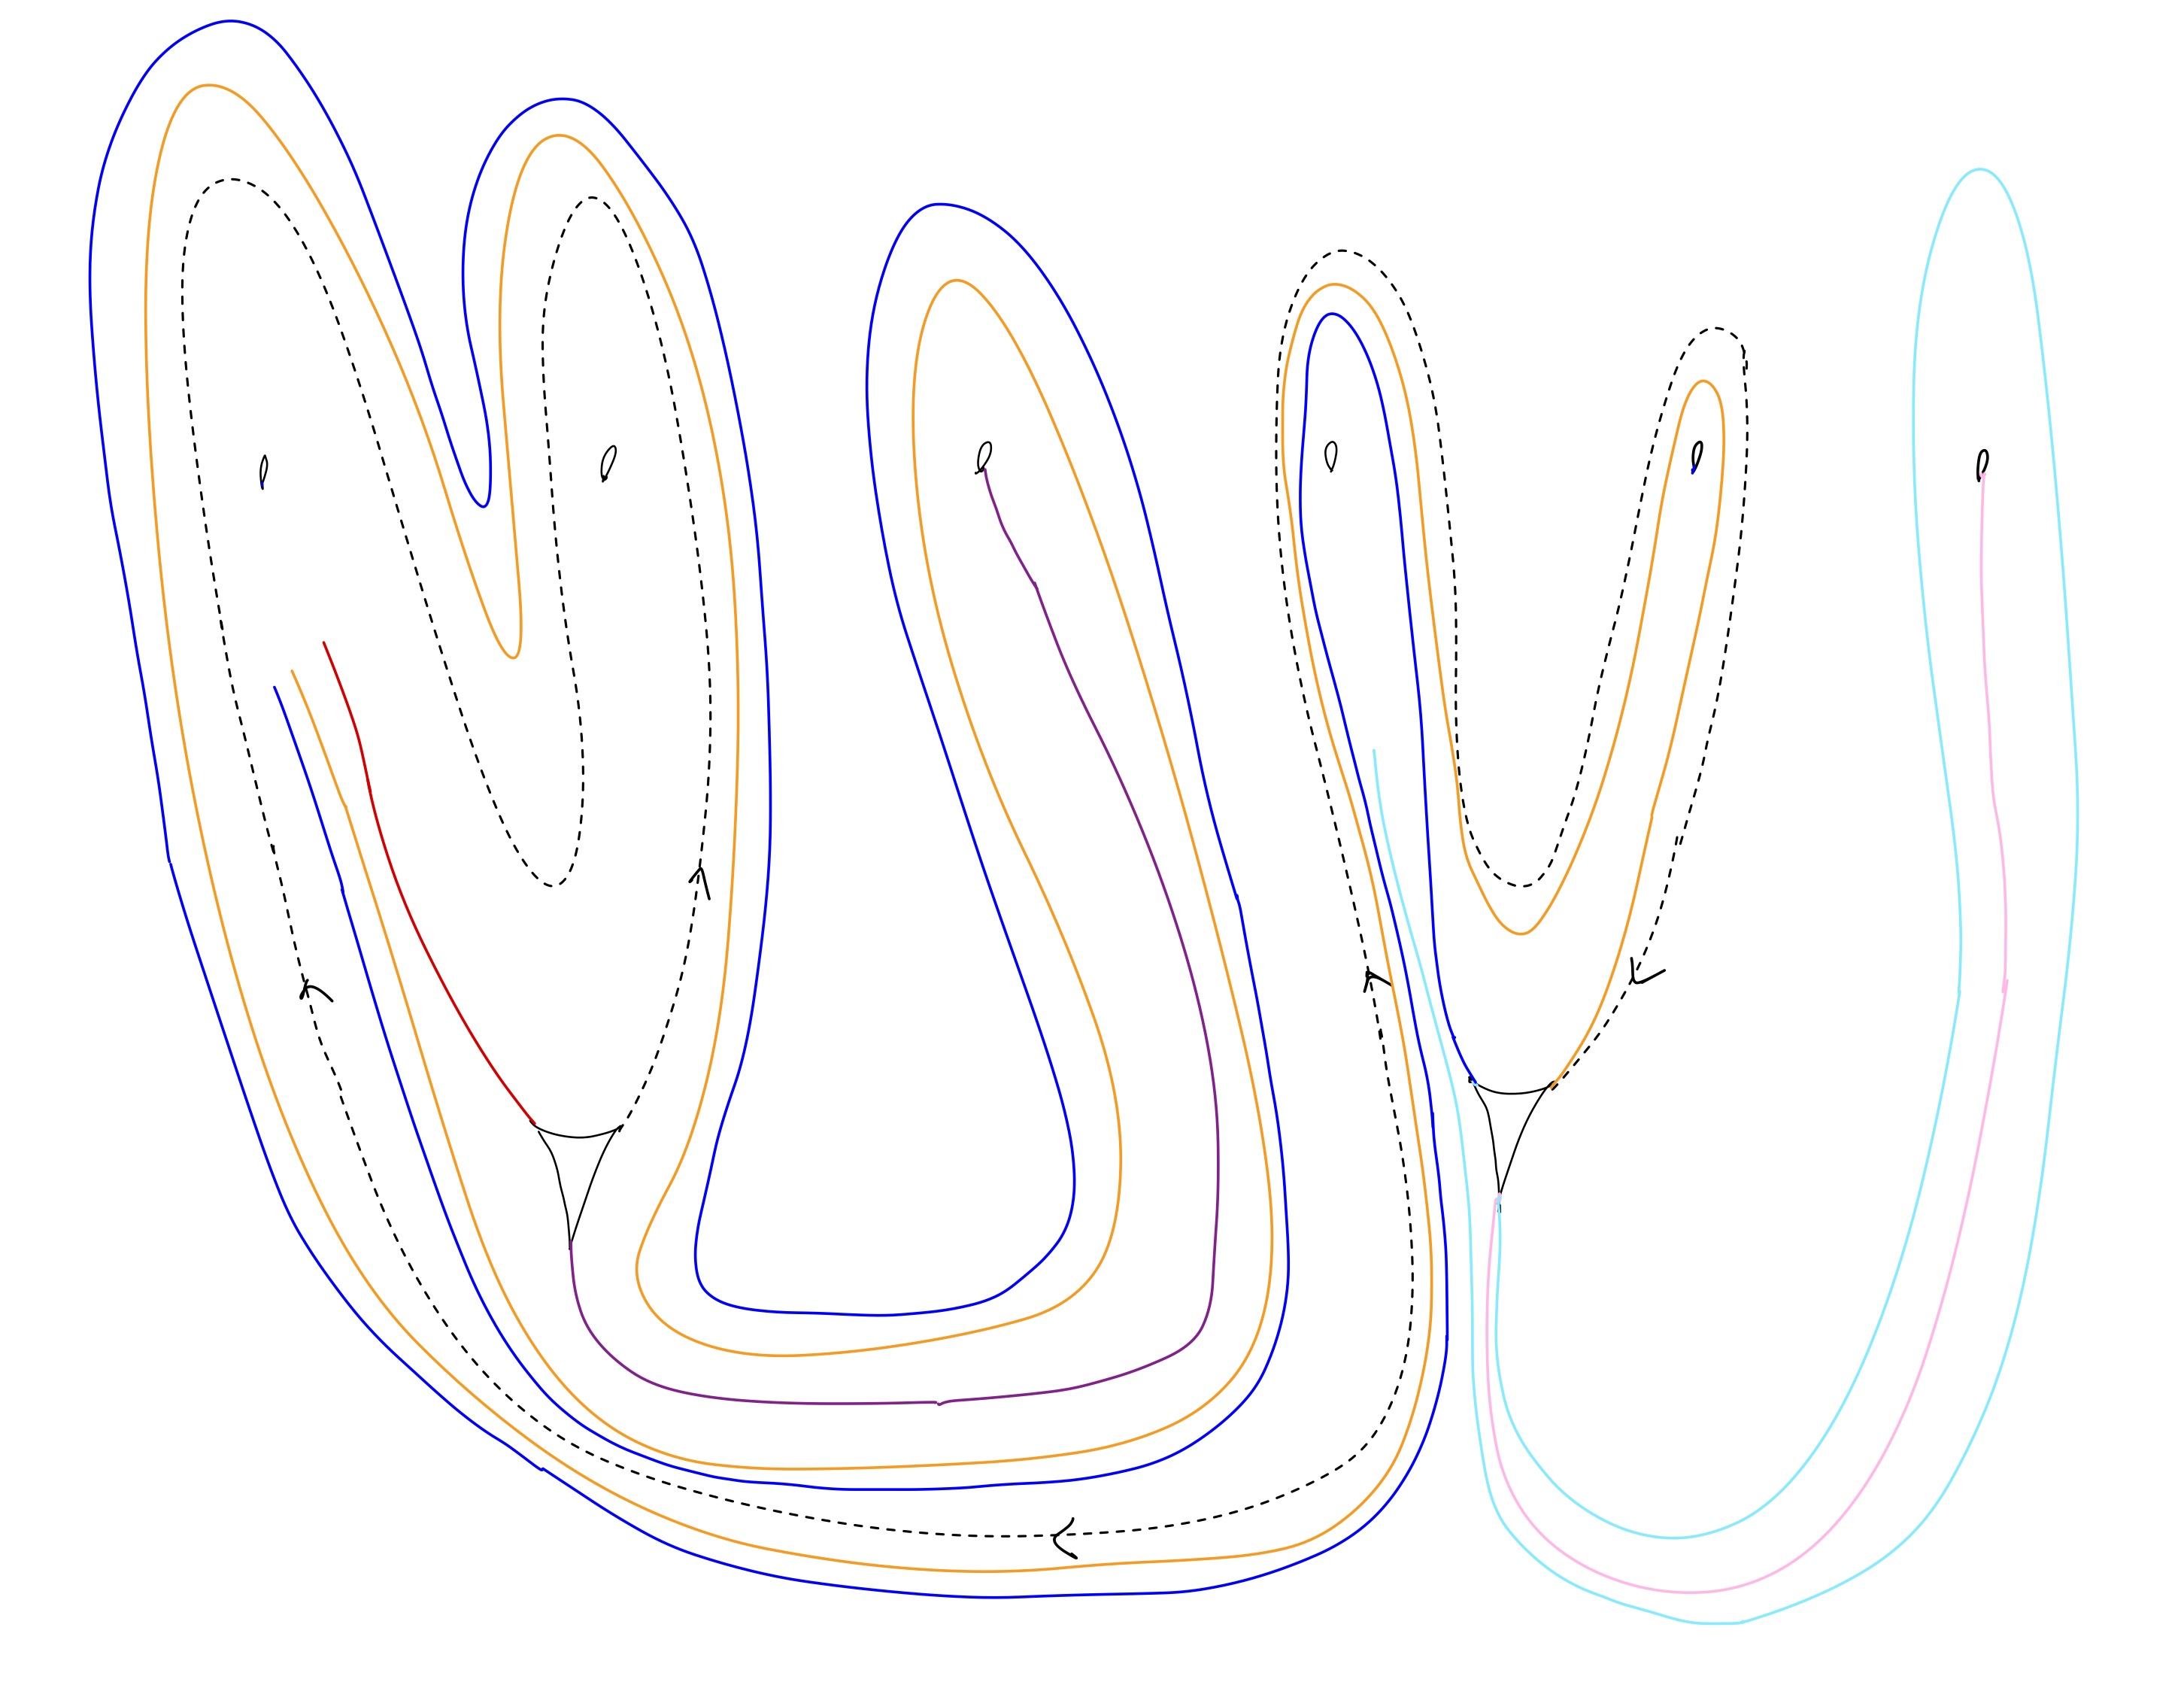
\includegraphics[width=\linewidth]{figures_case_analysis/track17_case_analysis/Flisky-03.jpg}
    \caption{Flisky3}
    \label{fig:Flisky3}
\end{figure}

\begin{figure}[ht]
    \centering
    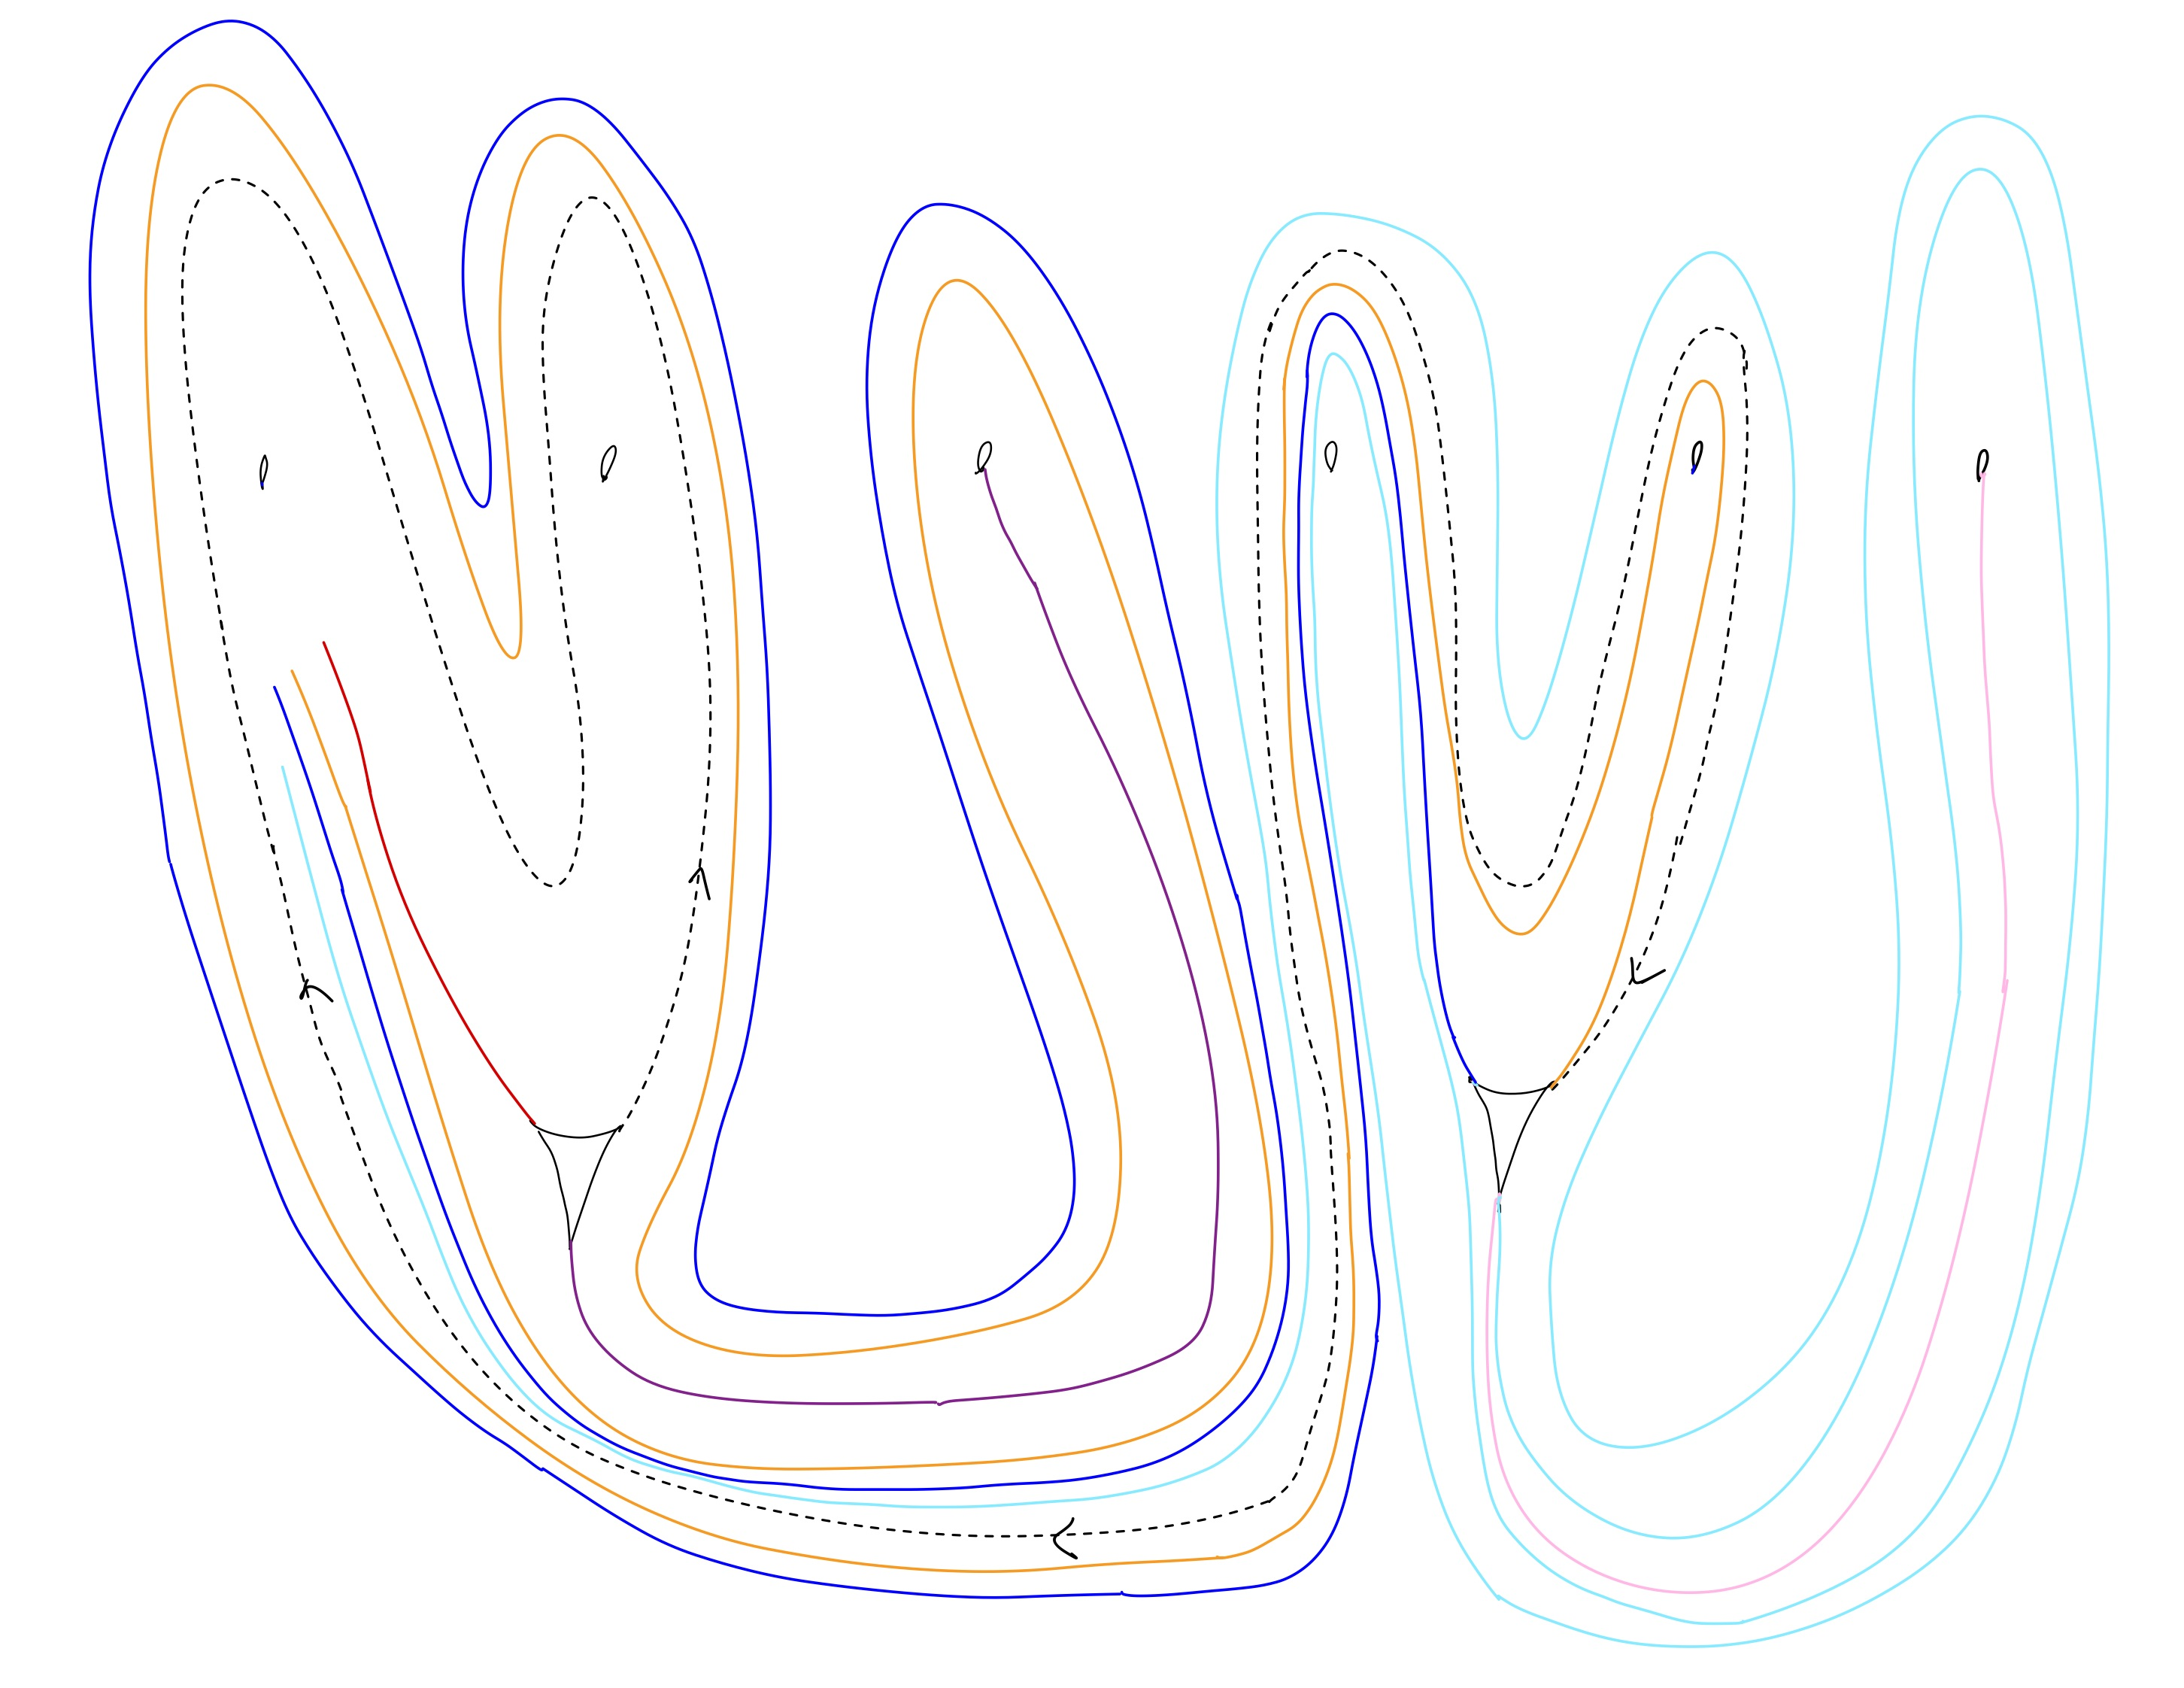
\includegraphics[width=\linewidth]{figures_case_analysis/track17_case_analysis/Flisky-04.jpg}
    \caption{Flisky4}
    \label{fig:Flisky4}
\end{figure}

\begin{figure}[ht]
    \centering
    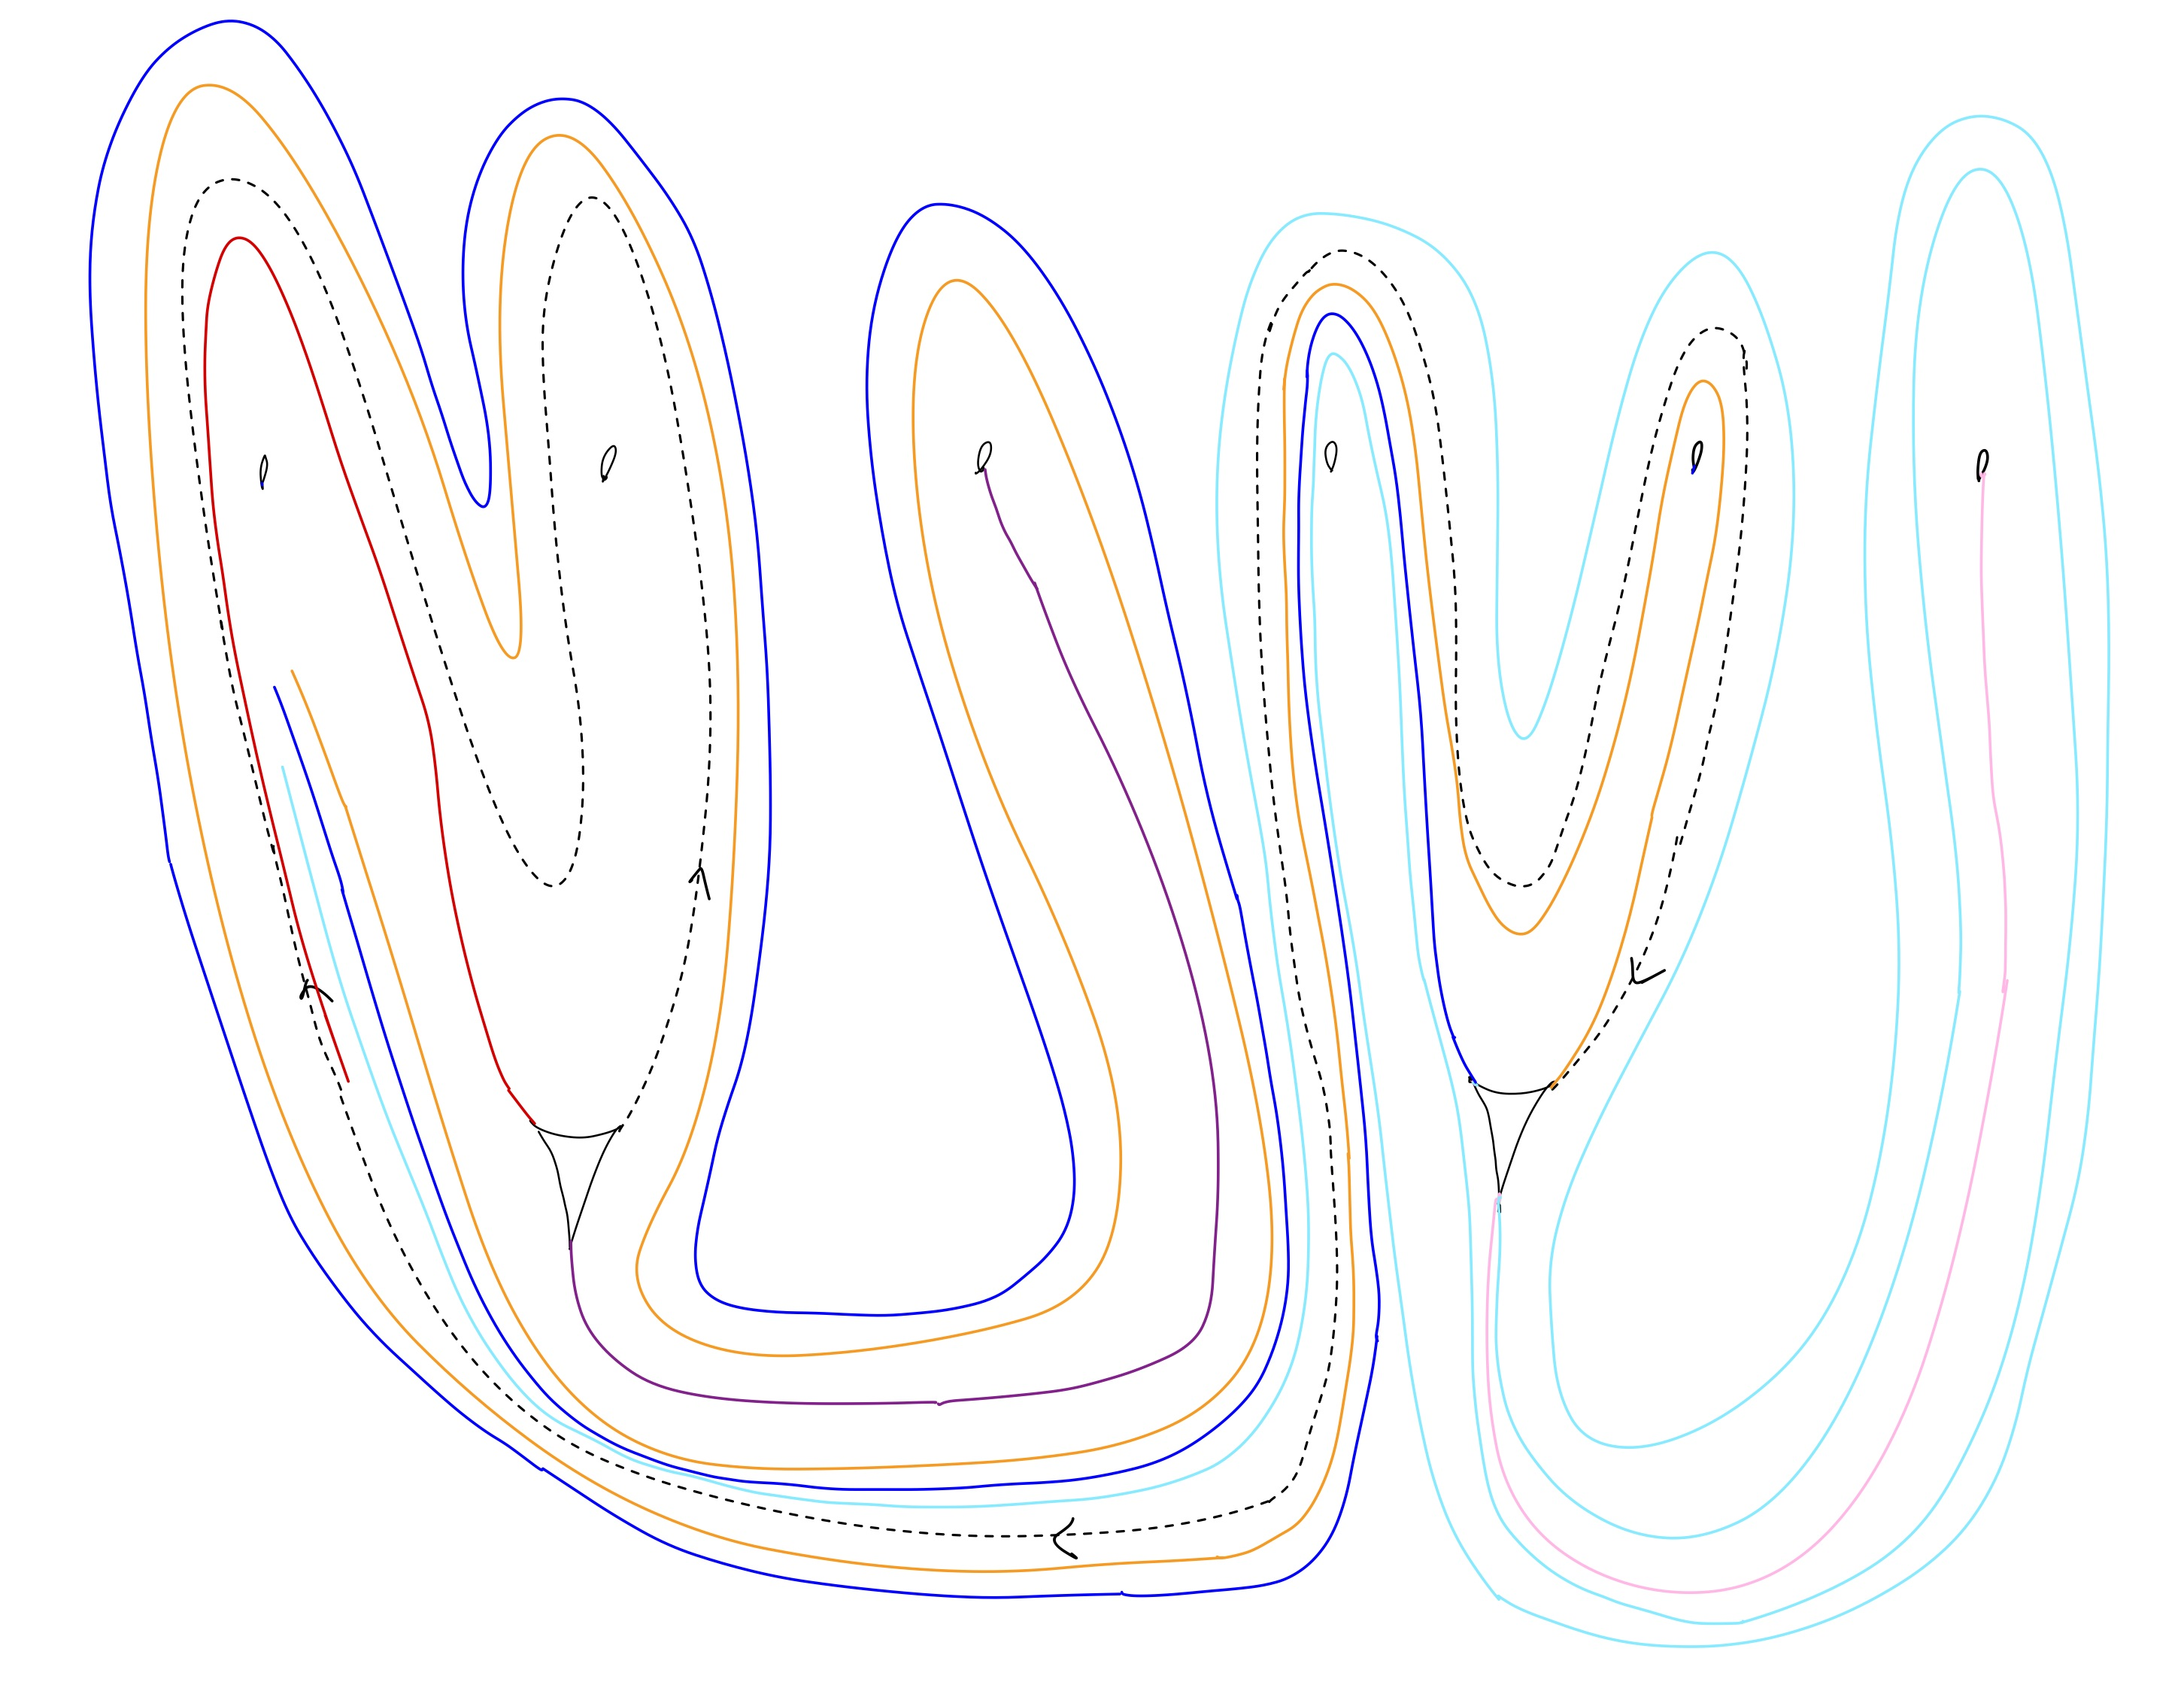
\includegraphics[width=\linewidth]{figures_case_analysis/track17_case_analysis/Flisky-05.jpg}
    \caption{Flisky5}
    \label{fig:Flisky5}
\end{figure}

\begin{figure}[ht]
    \centering
    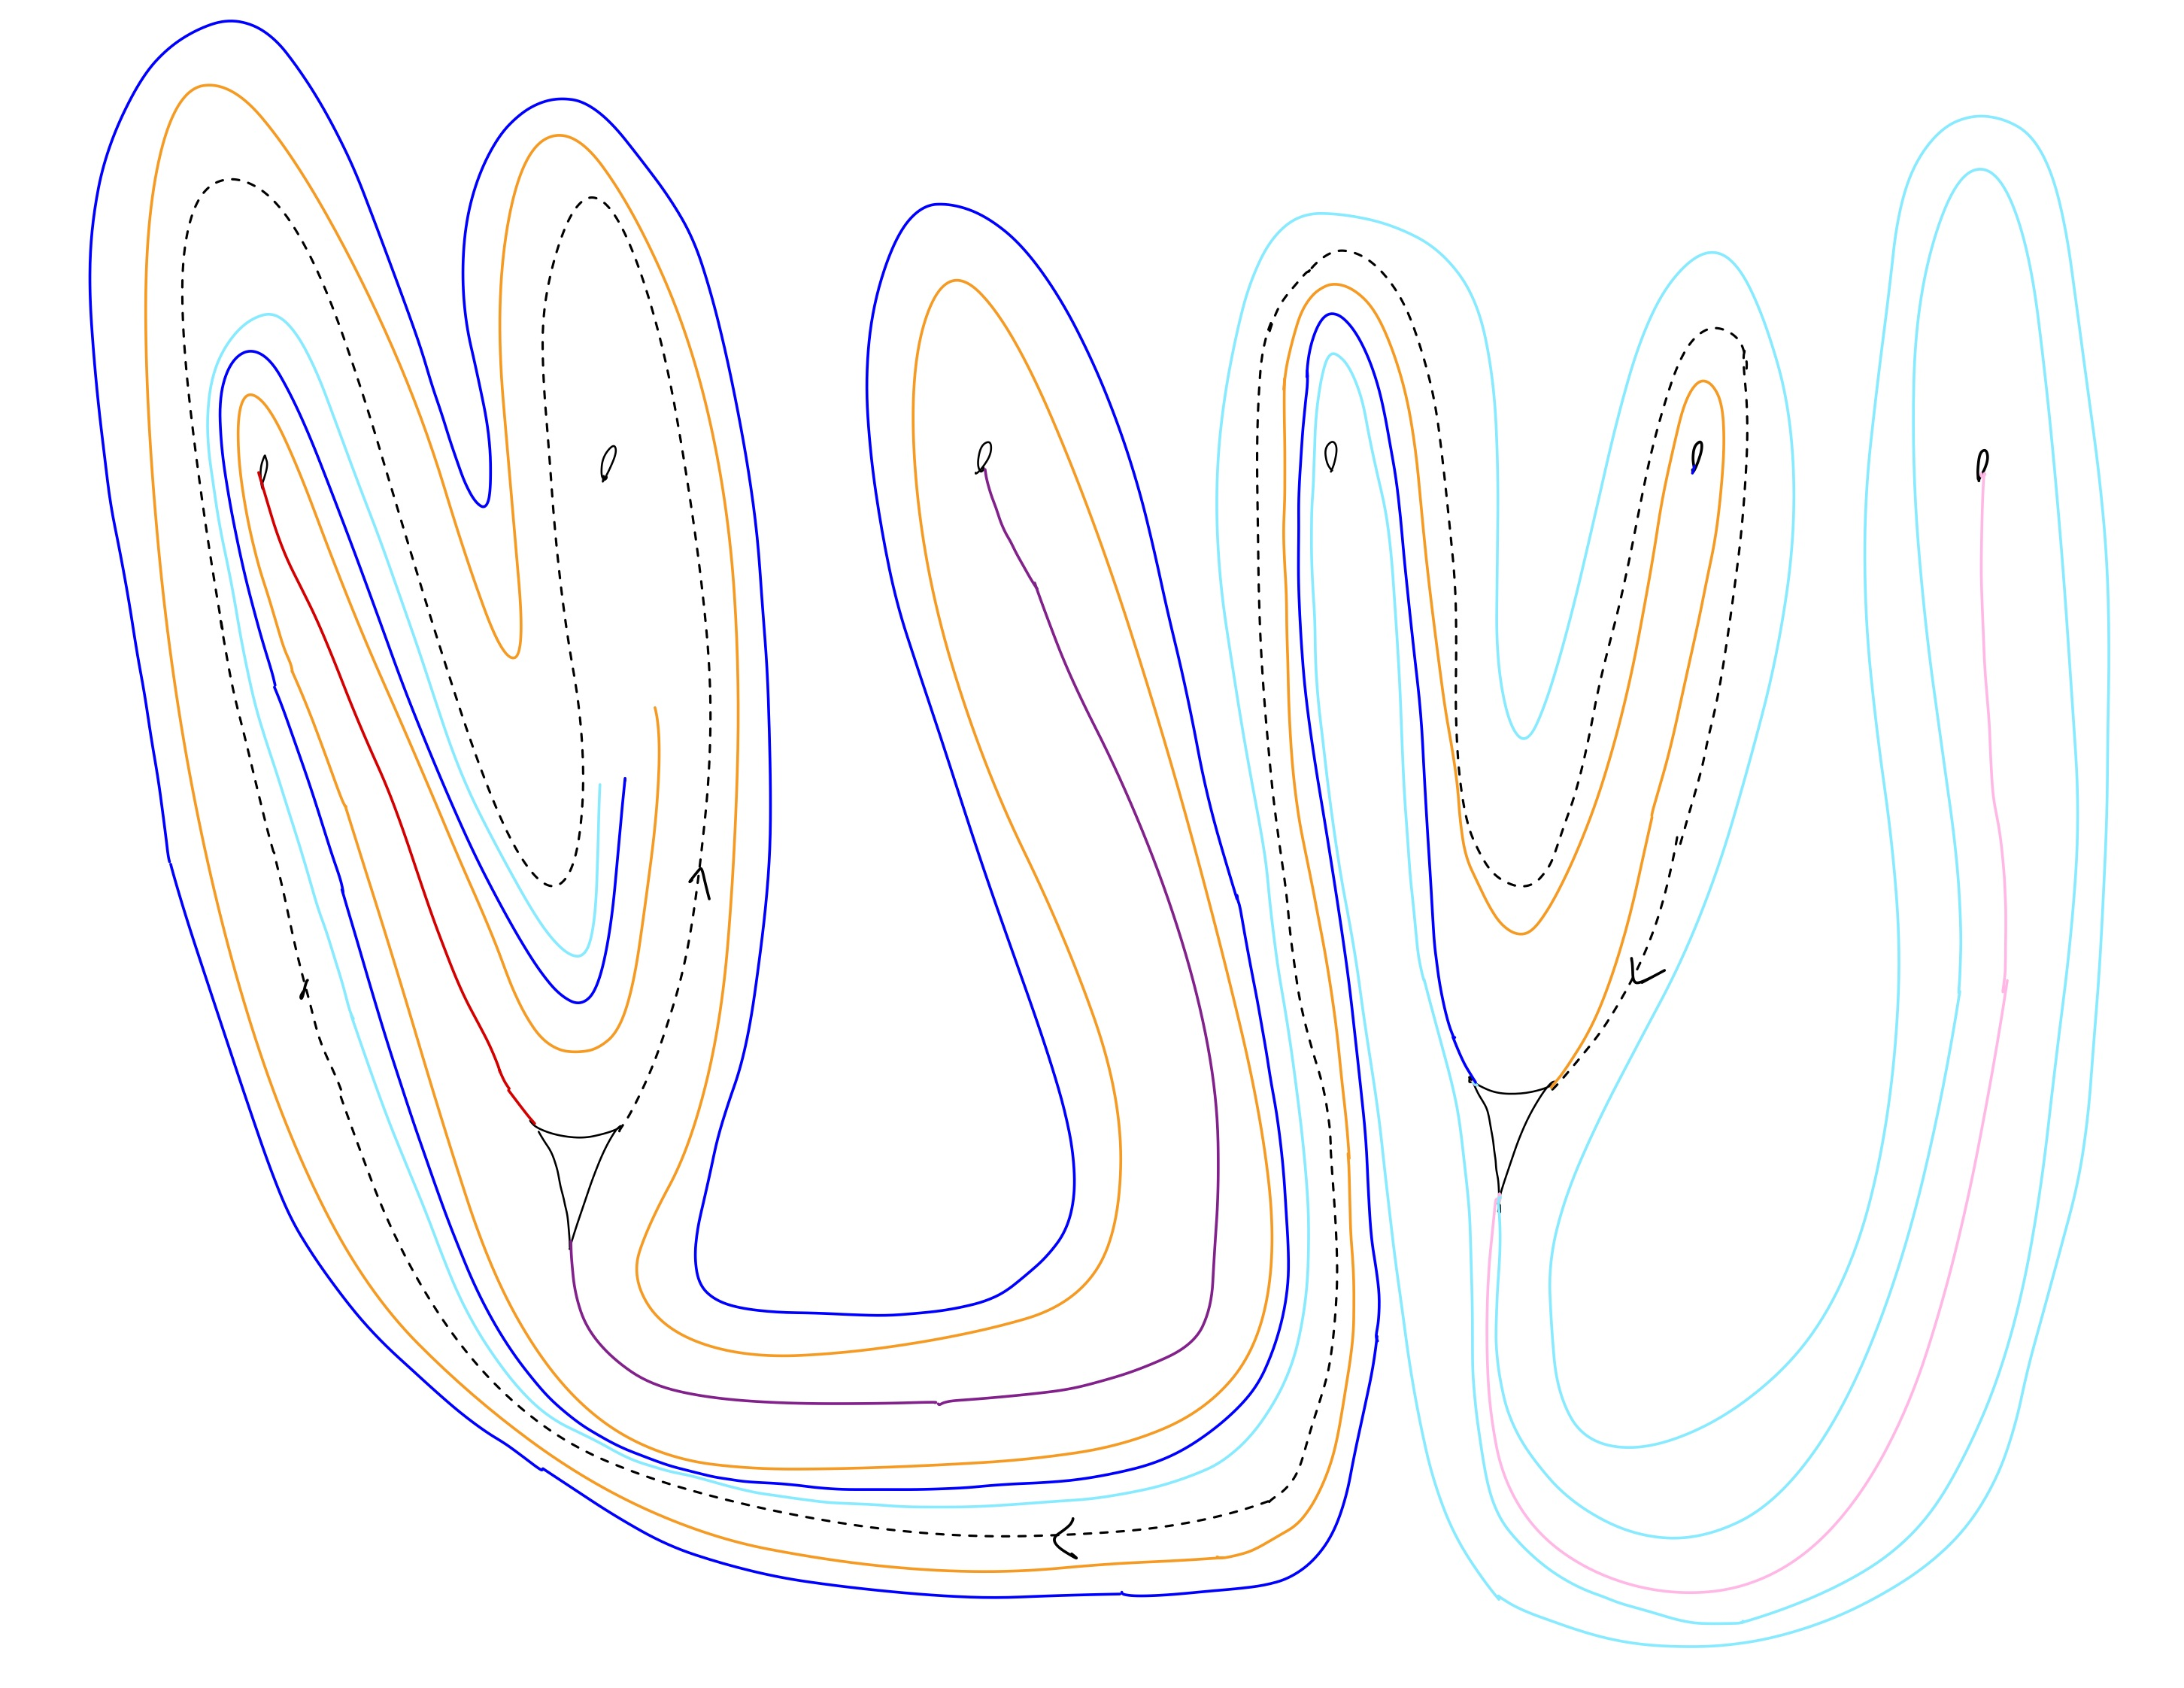
\includegraphics[width=\linewidth]{figures_case_analysis/track17_case_analysis/Flisky-06.jpg}
    \caption{Flisky6}
    \label{fig:Flisky6}
\end{figure}

\begin{figure}[ht]
    \centering
    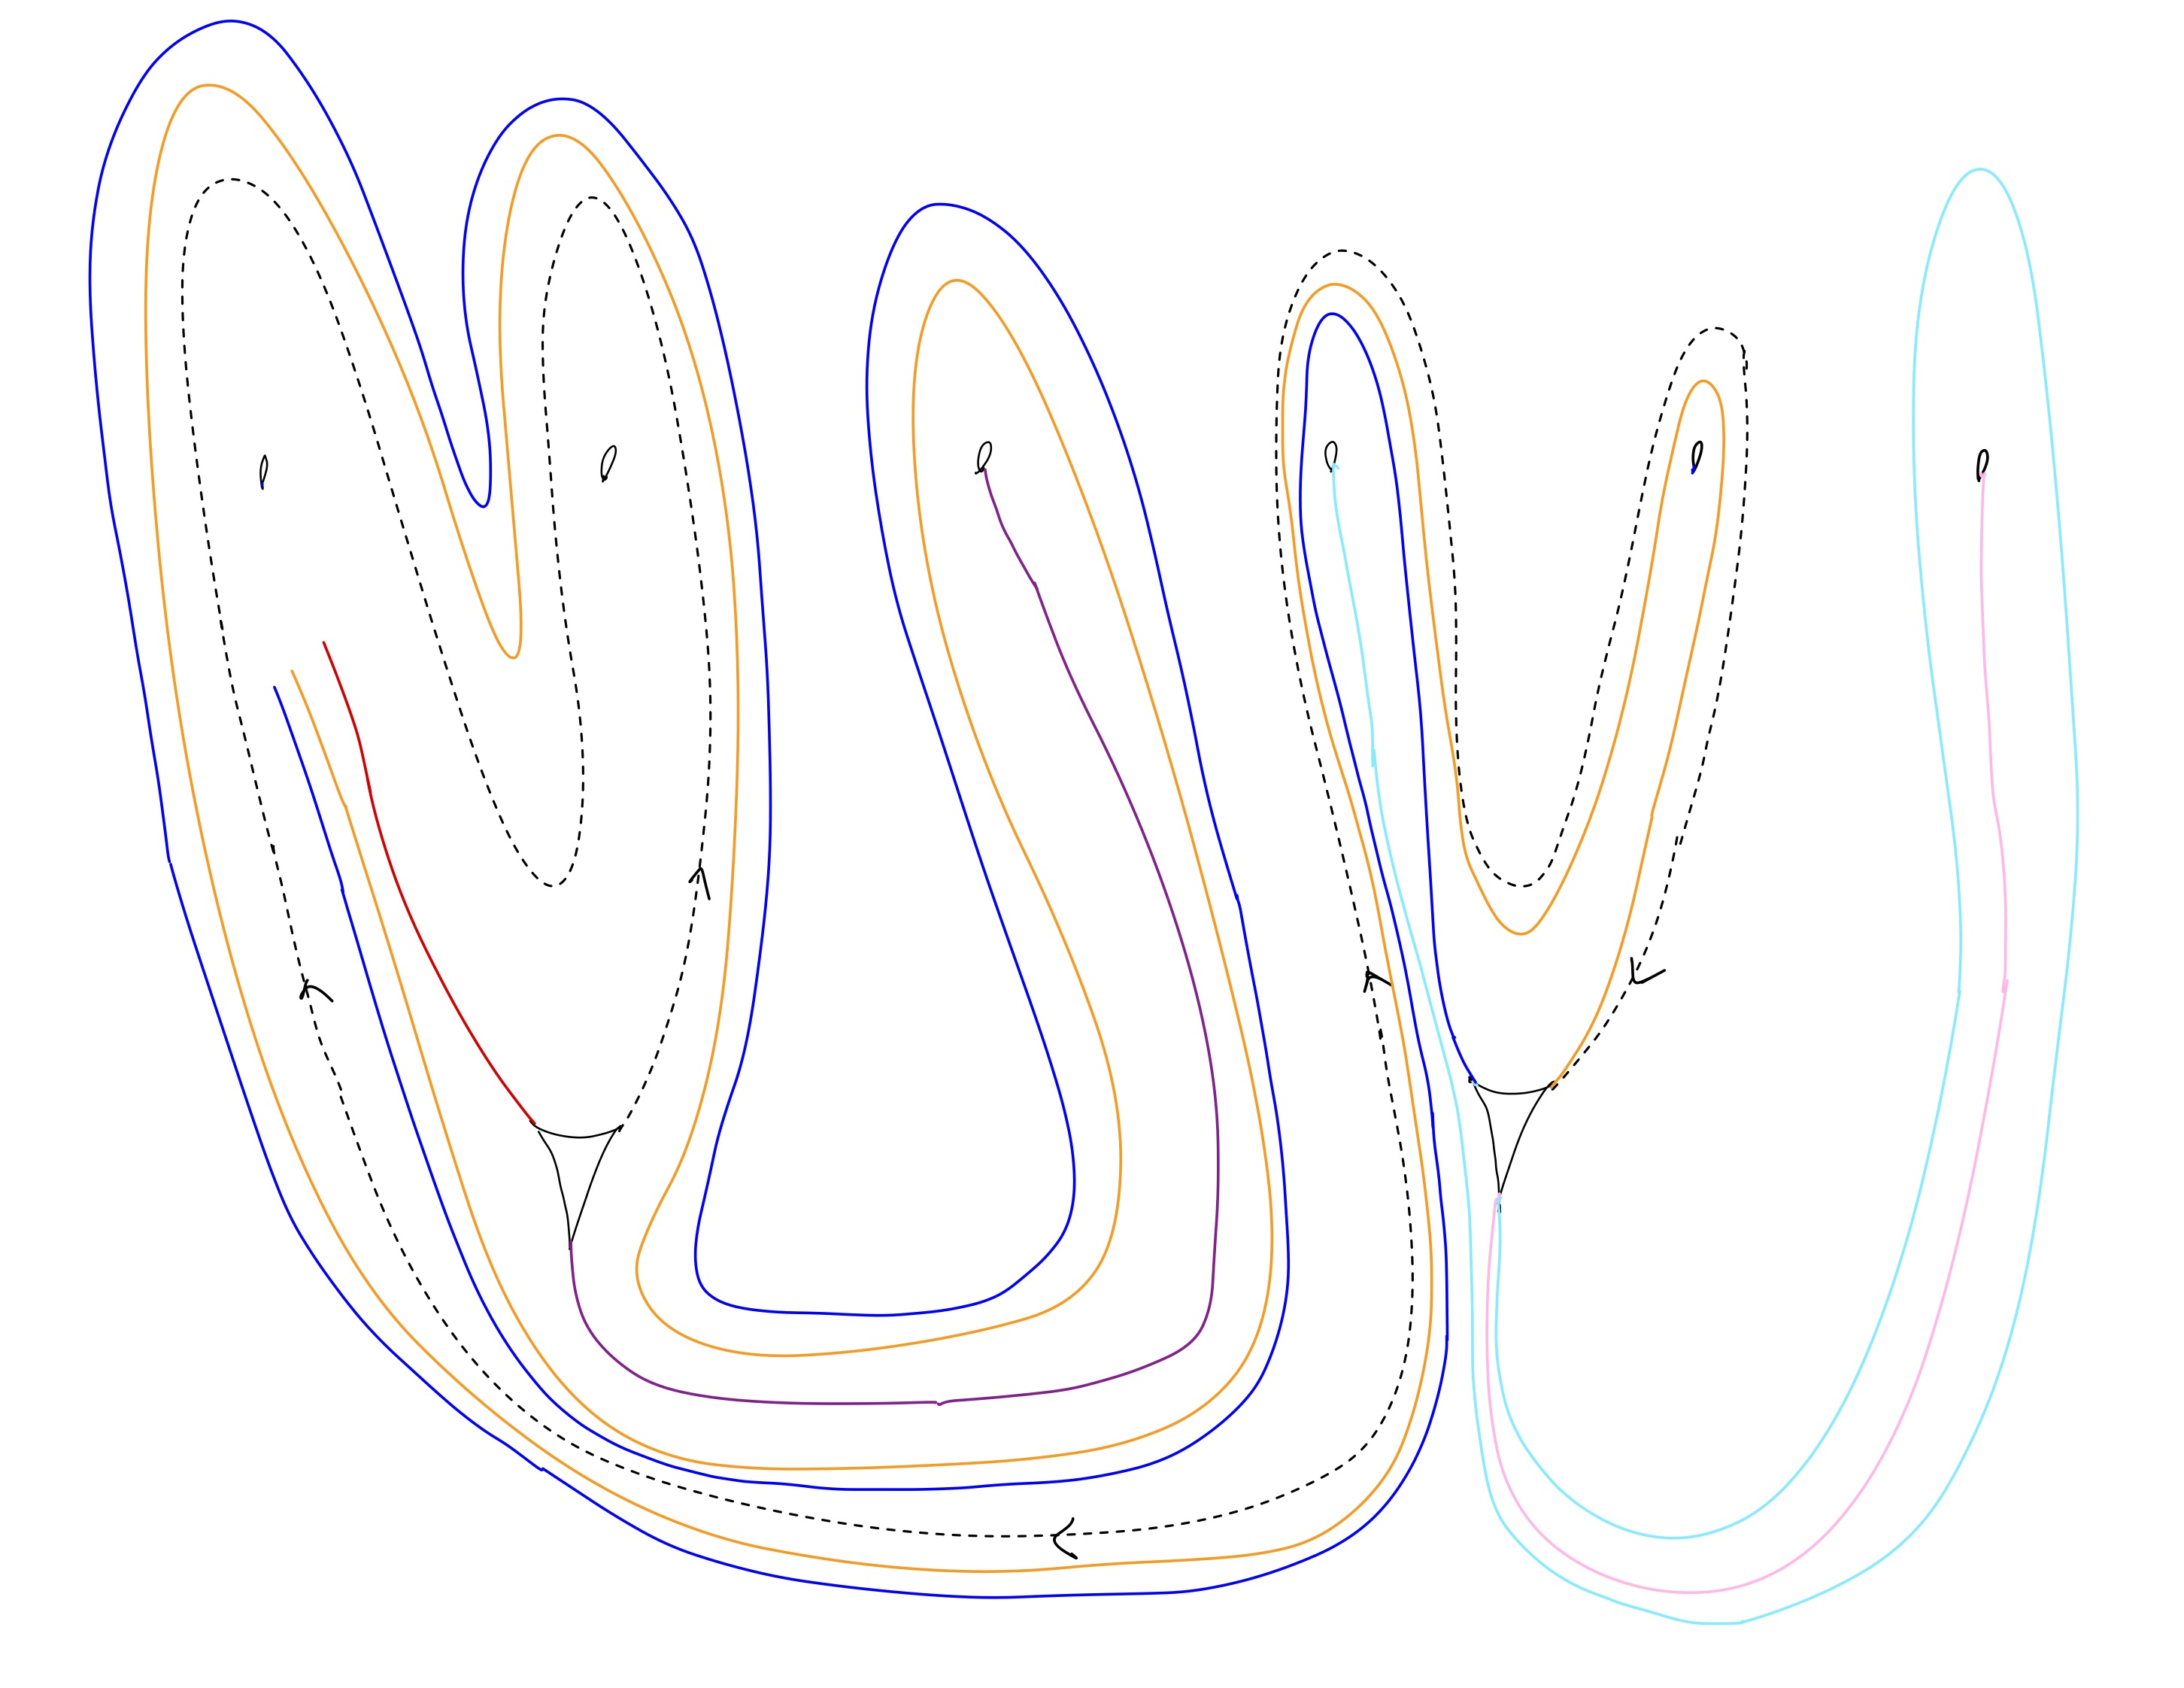
\includegraphics[width=\linewidth]{figures_case_analysis/track17_case_analysis/Flisky-07.jpg}
    \caption{Flisky7}
    \label{fig:Flisky7}
\end{figure}

\begin{figure}[ht]
    \centering
    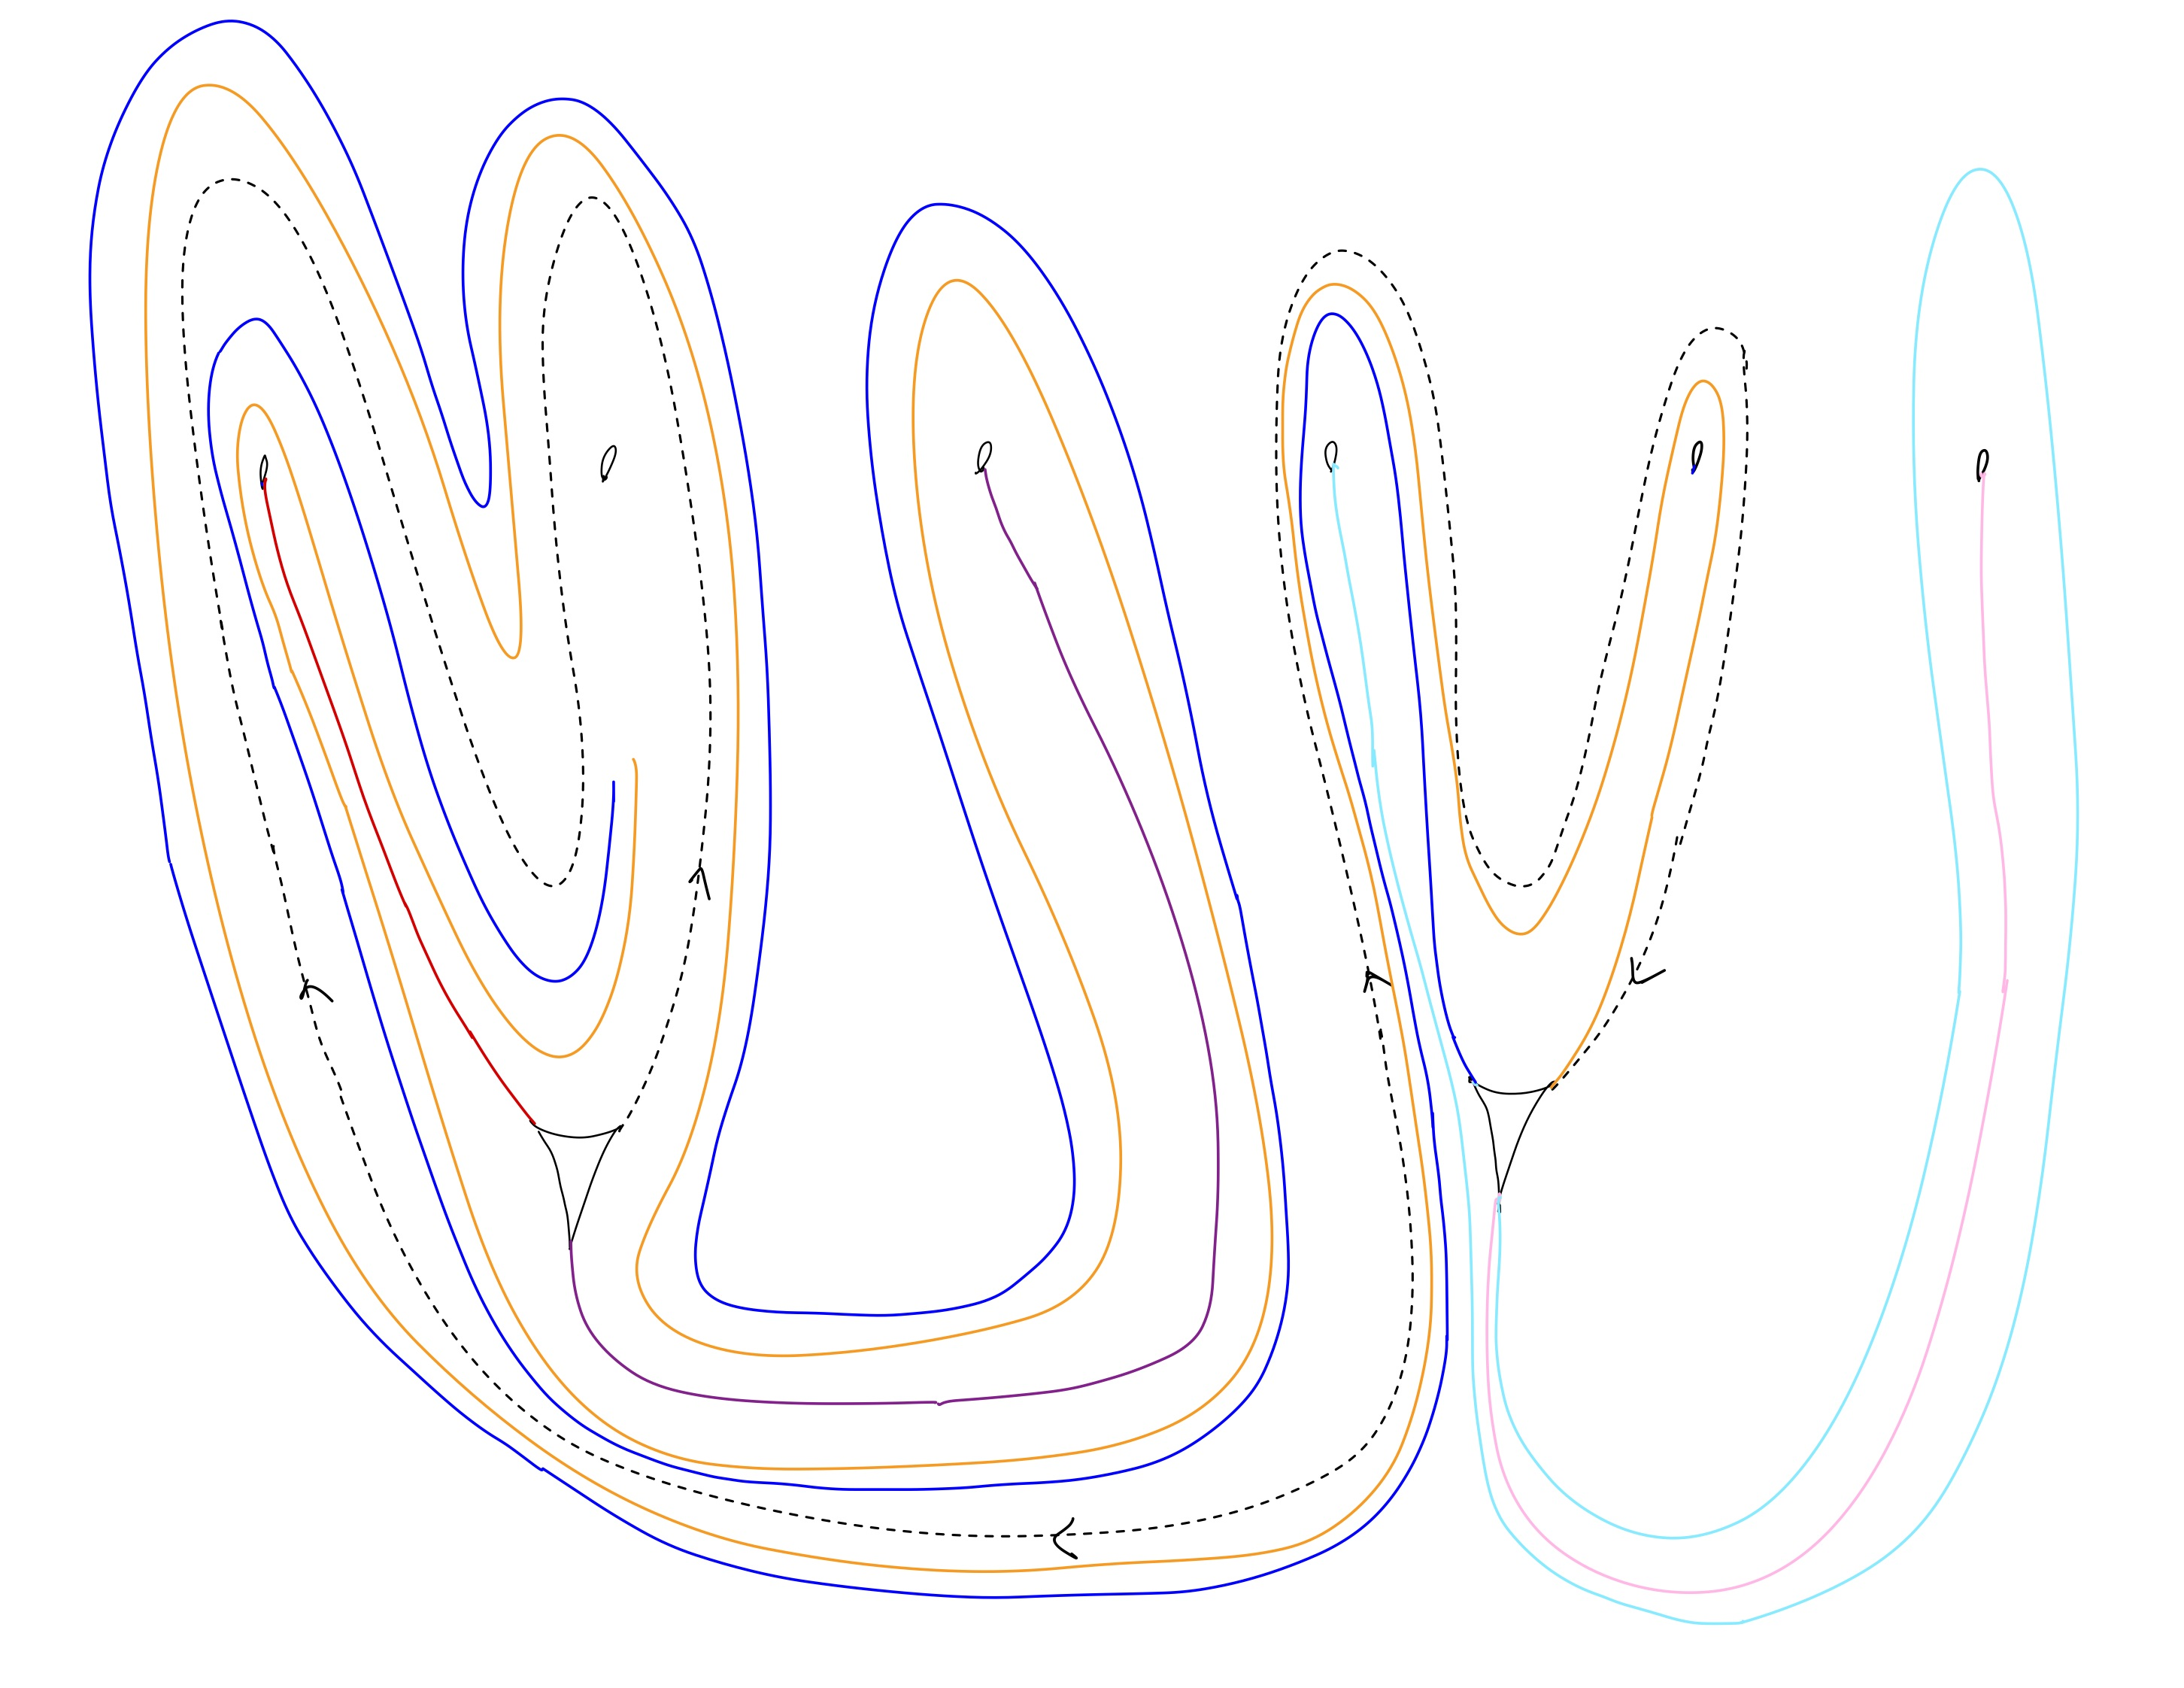
\includegraphics[width=\linewidth]{figures_case_analysis/track17_case_analysis/Flisky-08.jpg}
    \caption{Flisky8}
    \label{fig:Flisky8}
\end{figure}

\begin{figure}[ht]
    \centering
    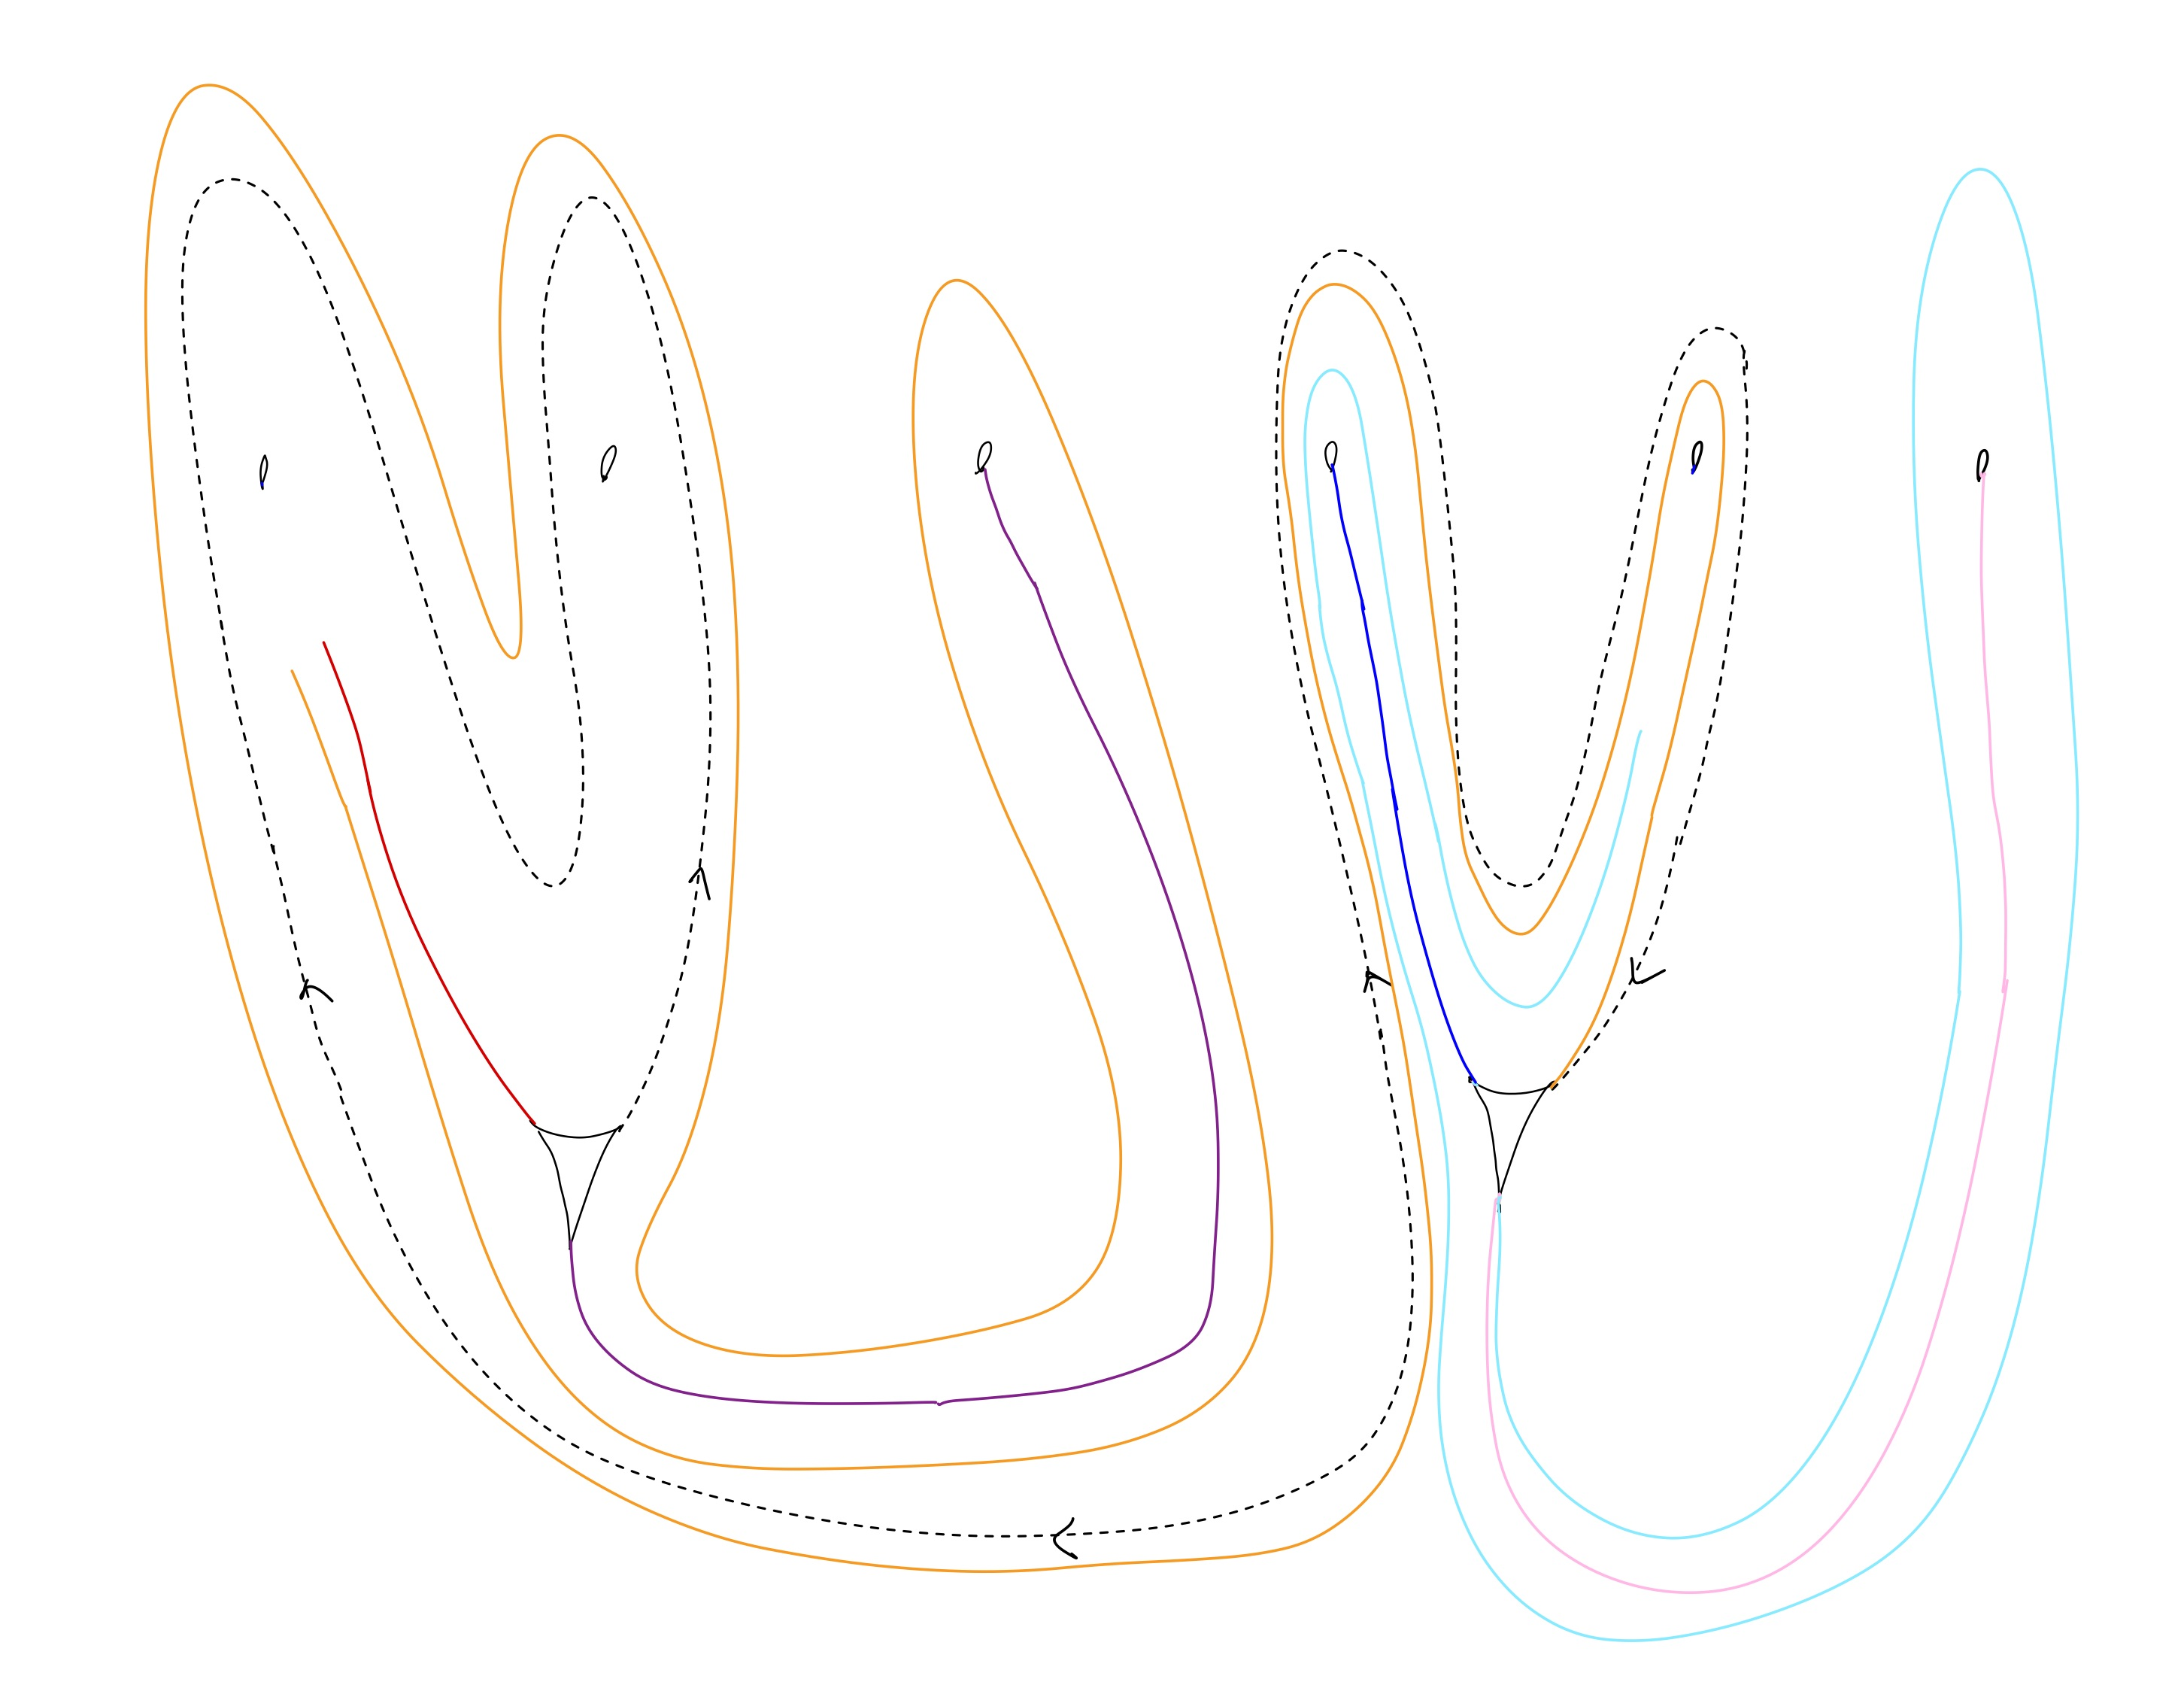
\includegraphics[width=\linewidth]{figures_case_analysis/track17_case_analysis/Flisky-09.jpg}
    \caption{Flisky9}
    \label{fig:Flisky9}
\end{figure}

\begin{figure}[ht]
    \centering
    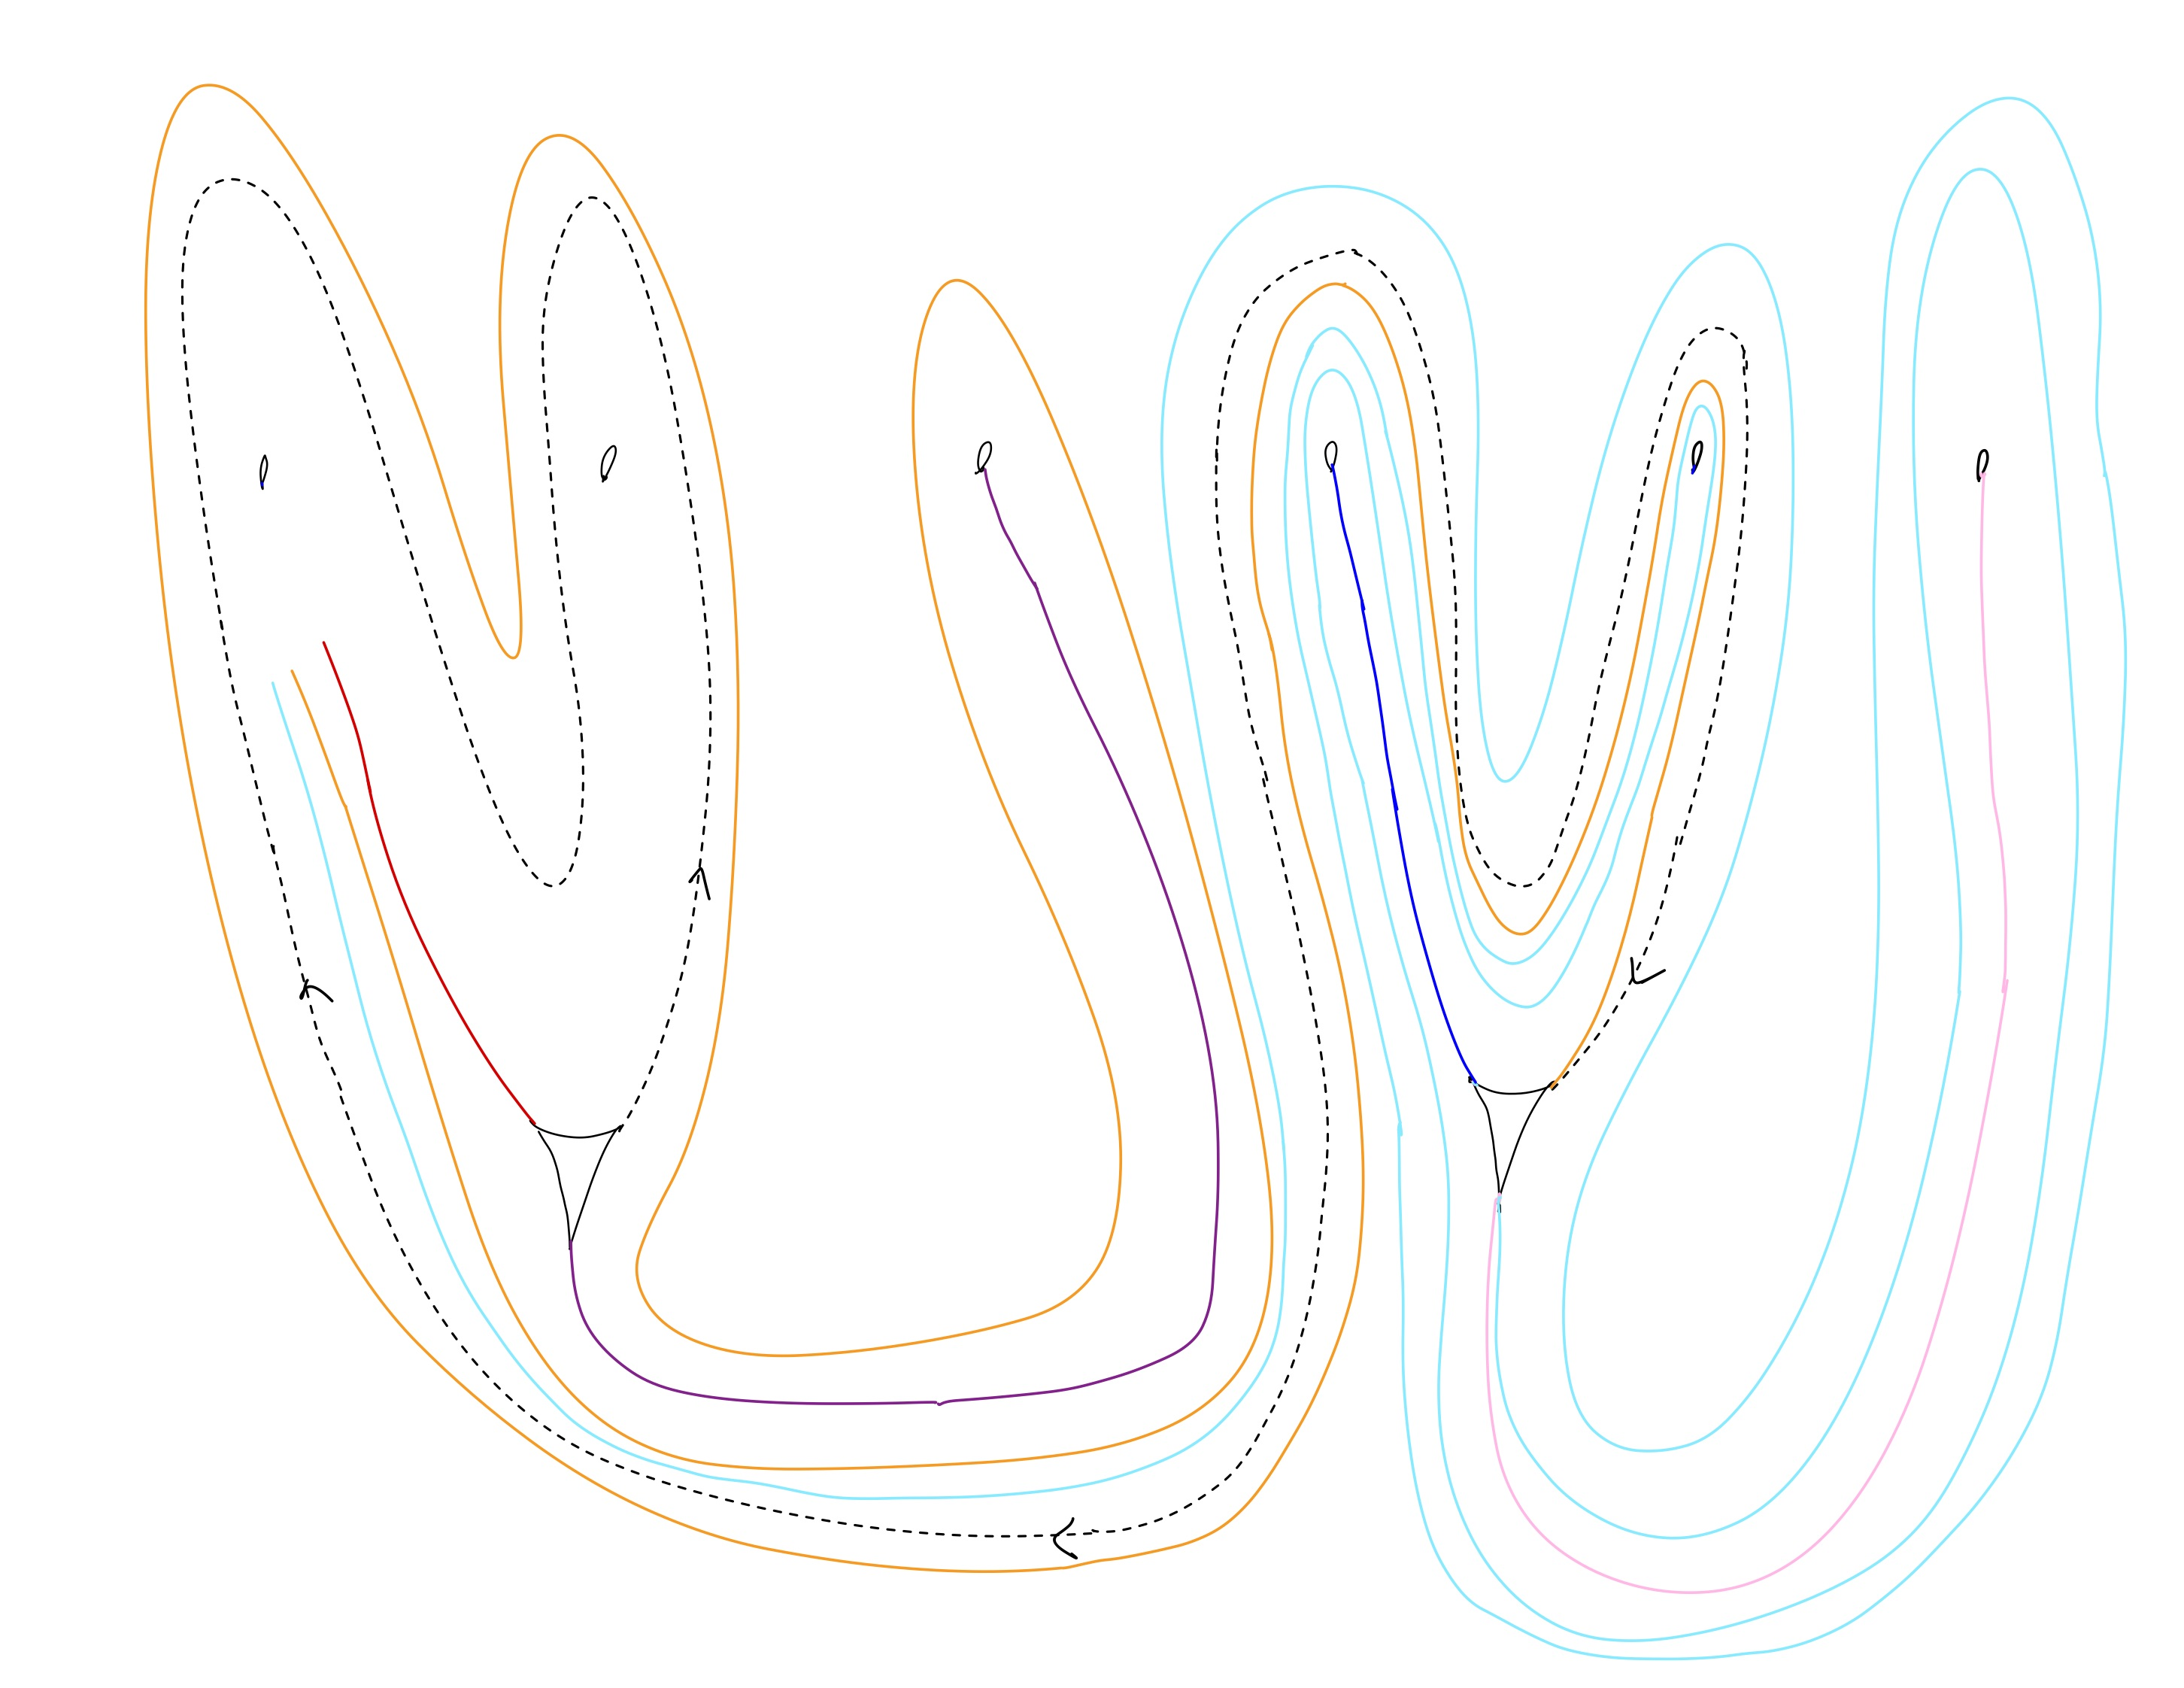
\includegraphics[width=\linewidth]{figures_case_analysis/track17_case_analysis/Flisky-10.jpg}
    \caption{Flisky10}
    \label{fig:Flisky10}
\end{figure}

\begin{figure}[ht]
    \centering
    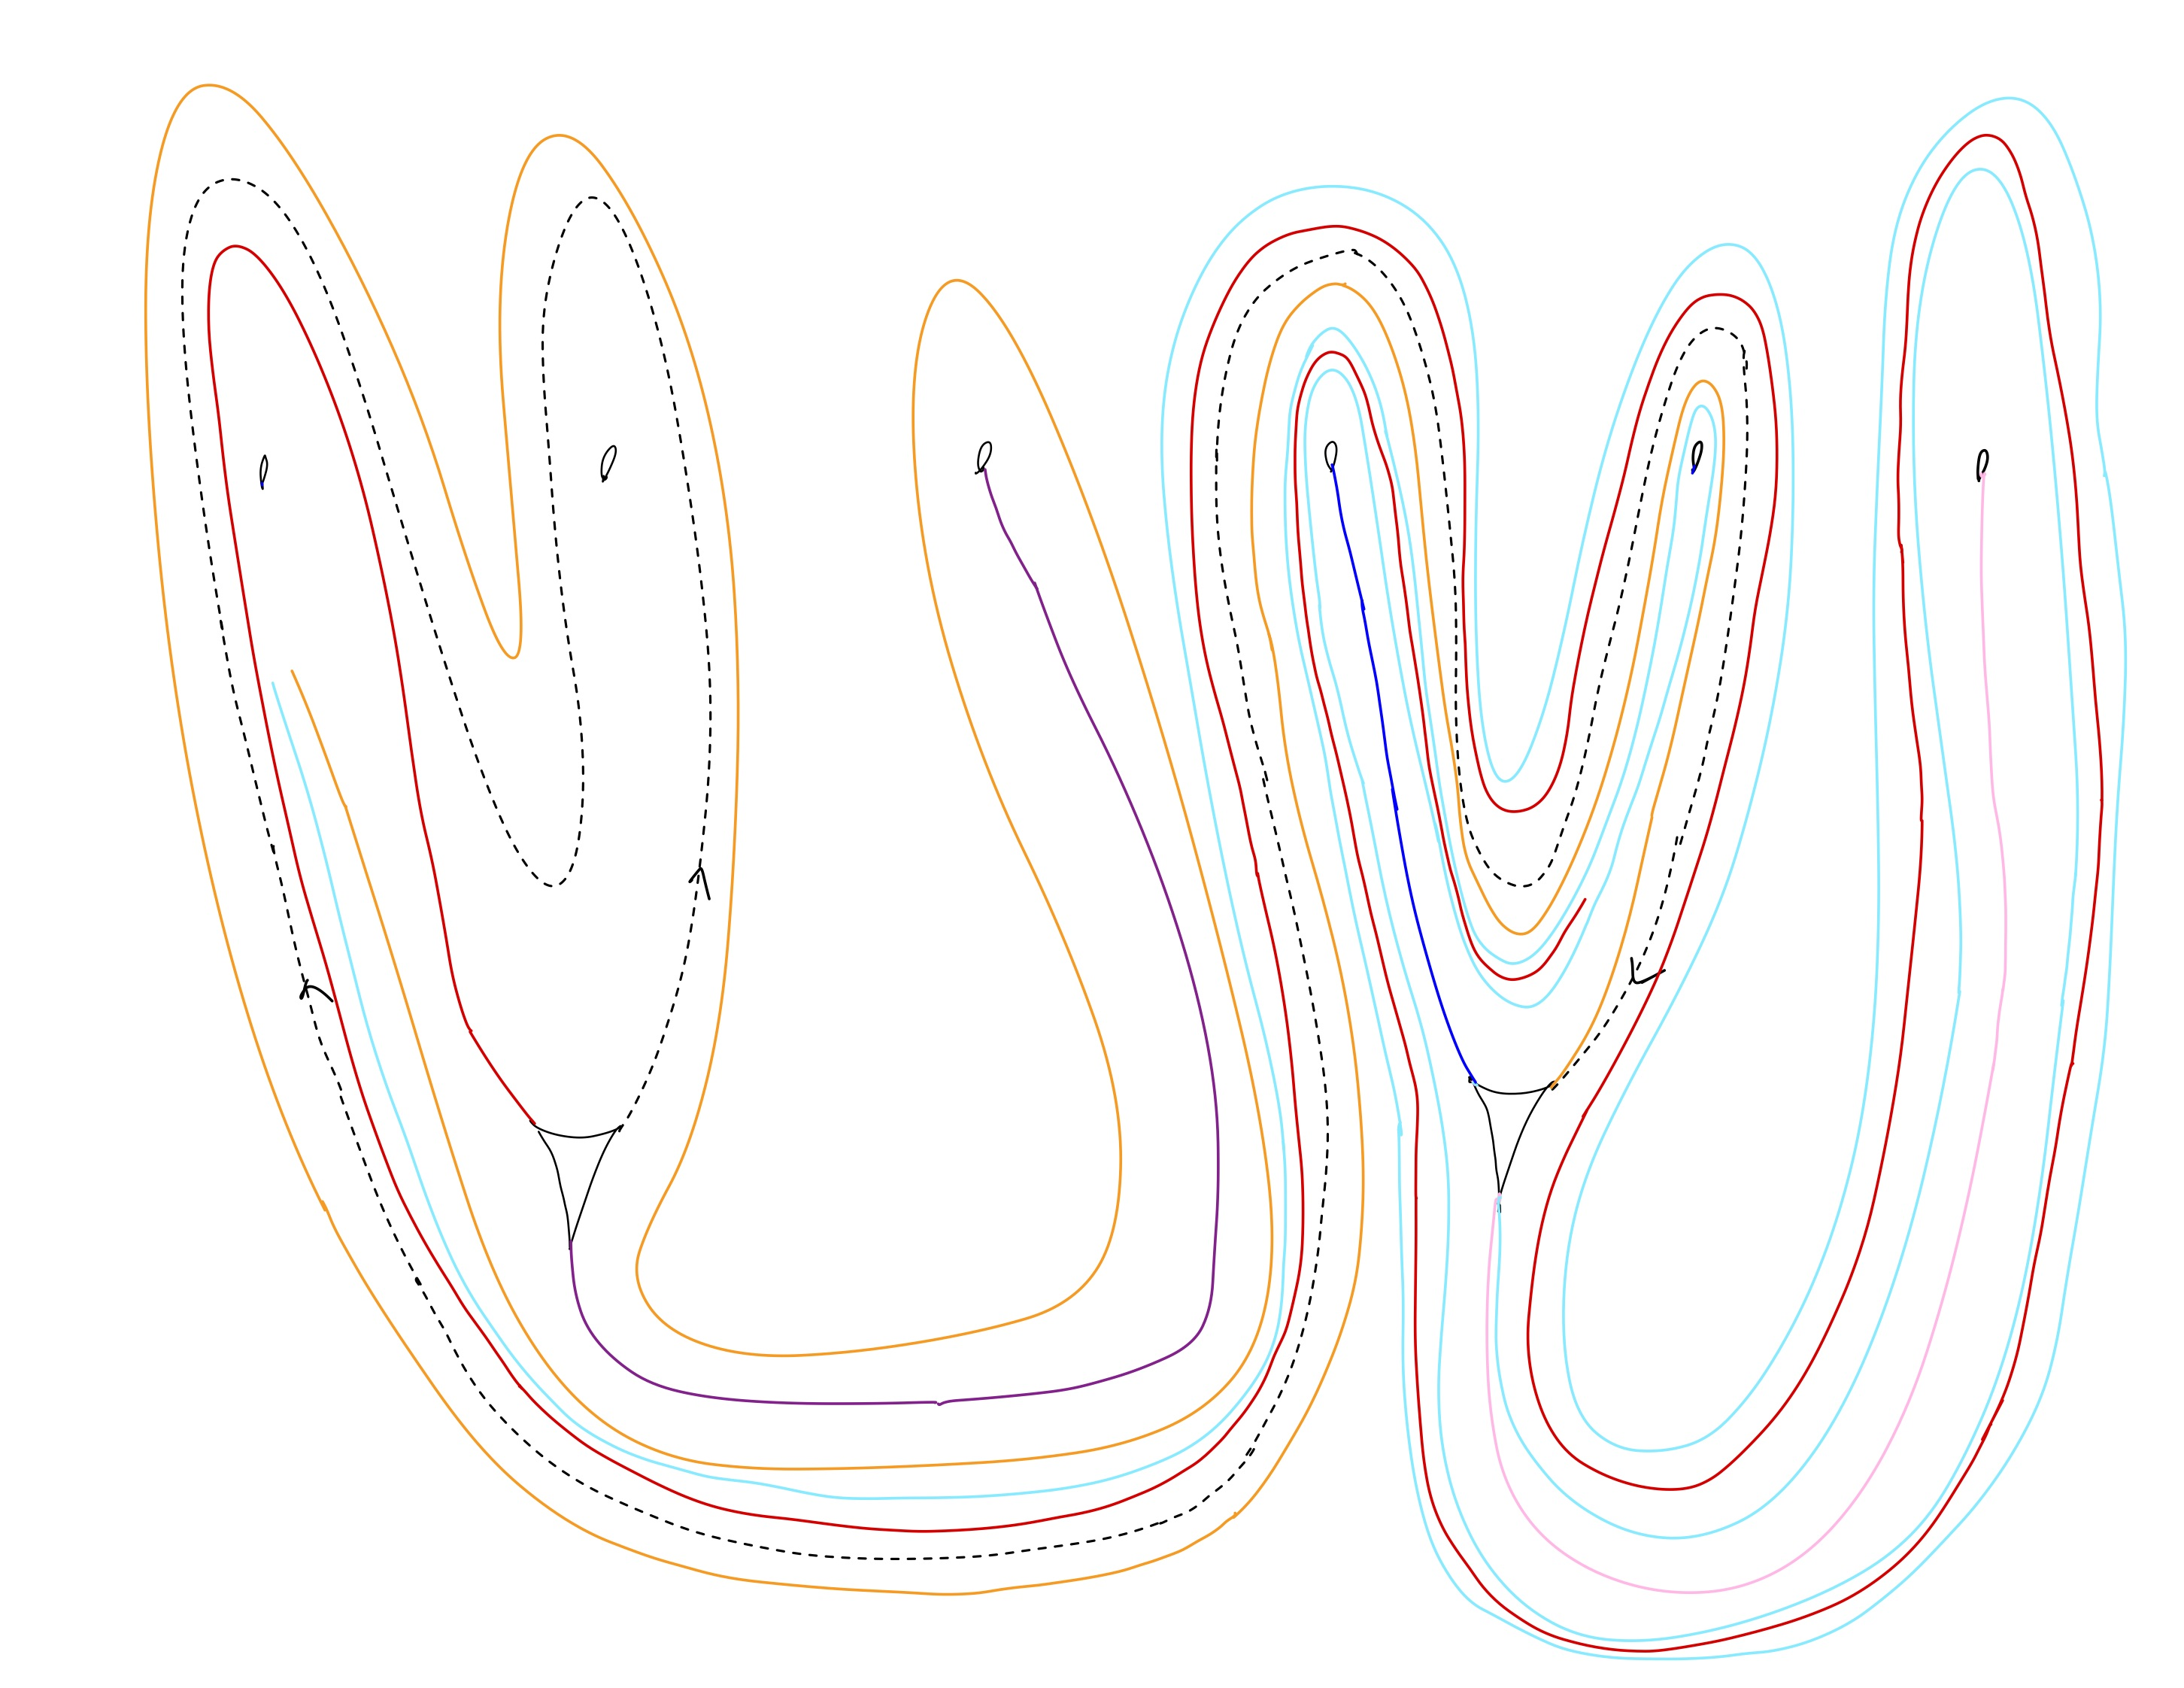
\includegraphics[width=\linewidth]{figures_case_analysis/track17_case_analysis/Flisky-11.jpg}
    \caption{Flisky11}
    \label{fig:Flisky11}
\end{figure}

\begin{figure}[ht]
    \centering
    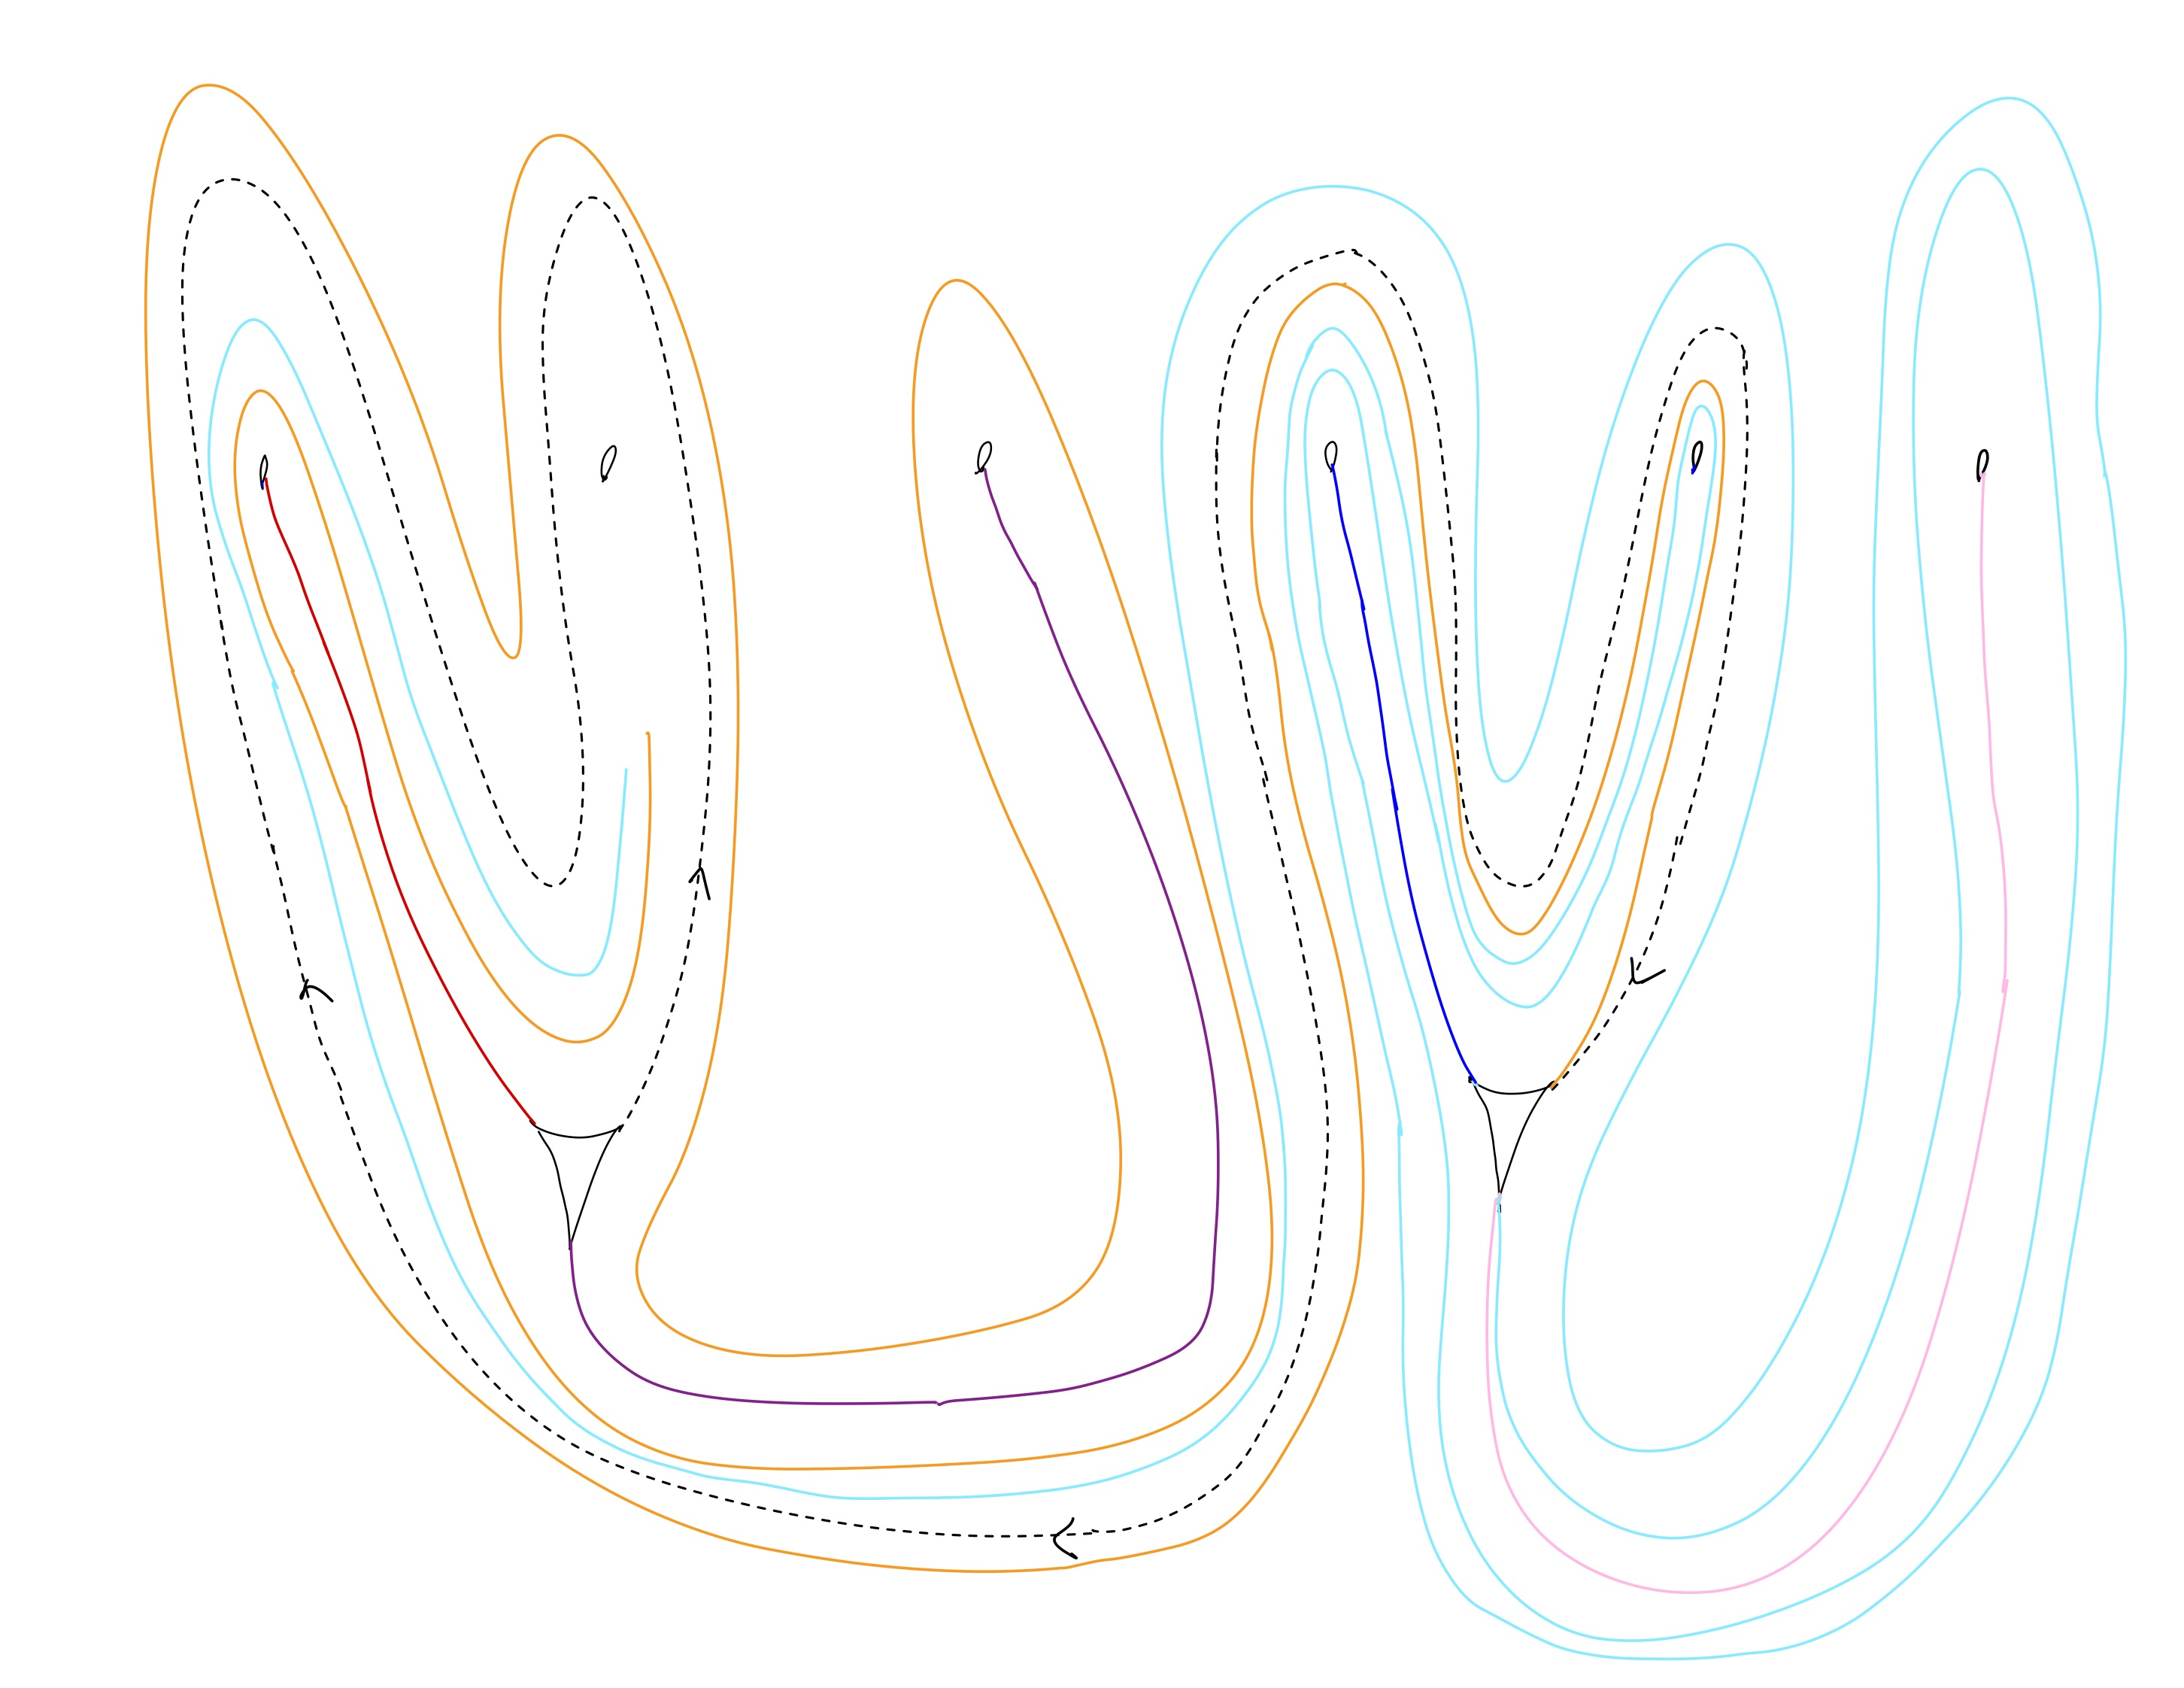
\includegraphics[width=\linewidth]{figures_case_analysis/track17_case_analysis/Flisky-12.jpg}
    \caption{Flisky12}
    \label{fig:Flisky12}
\end{figure}

\begin{figure}[ht]
    \centering
    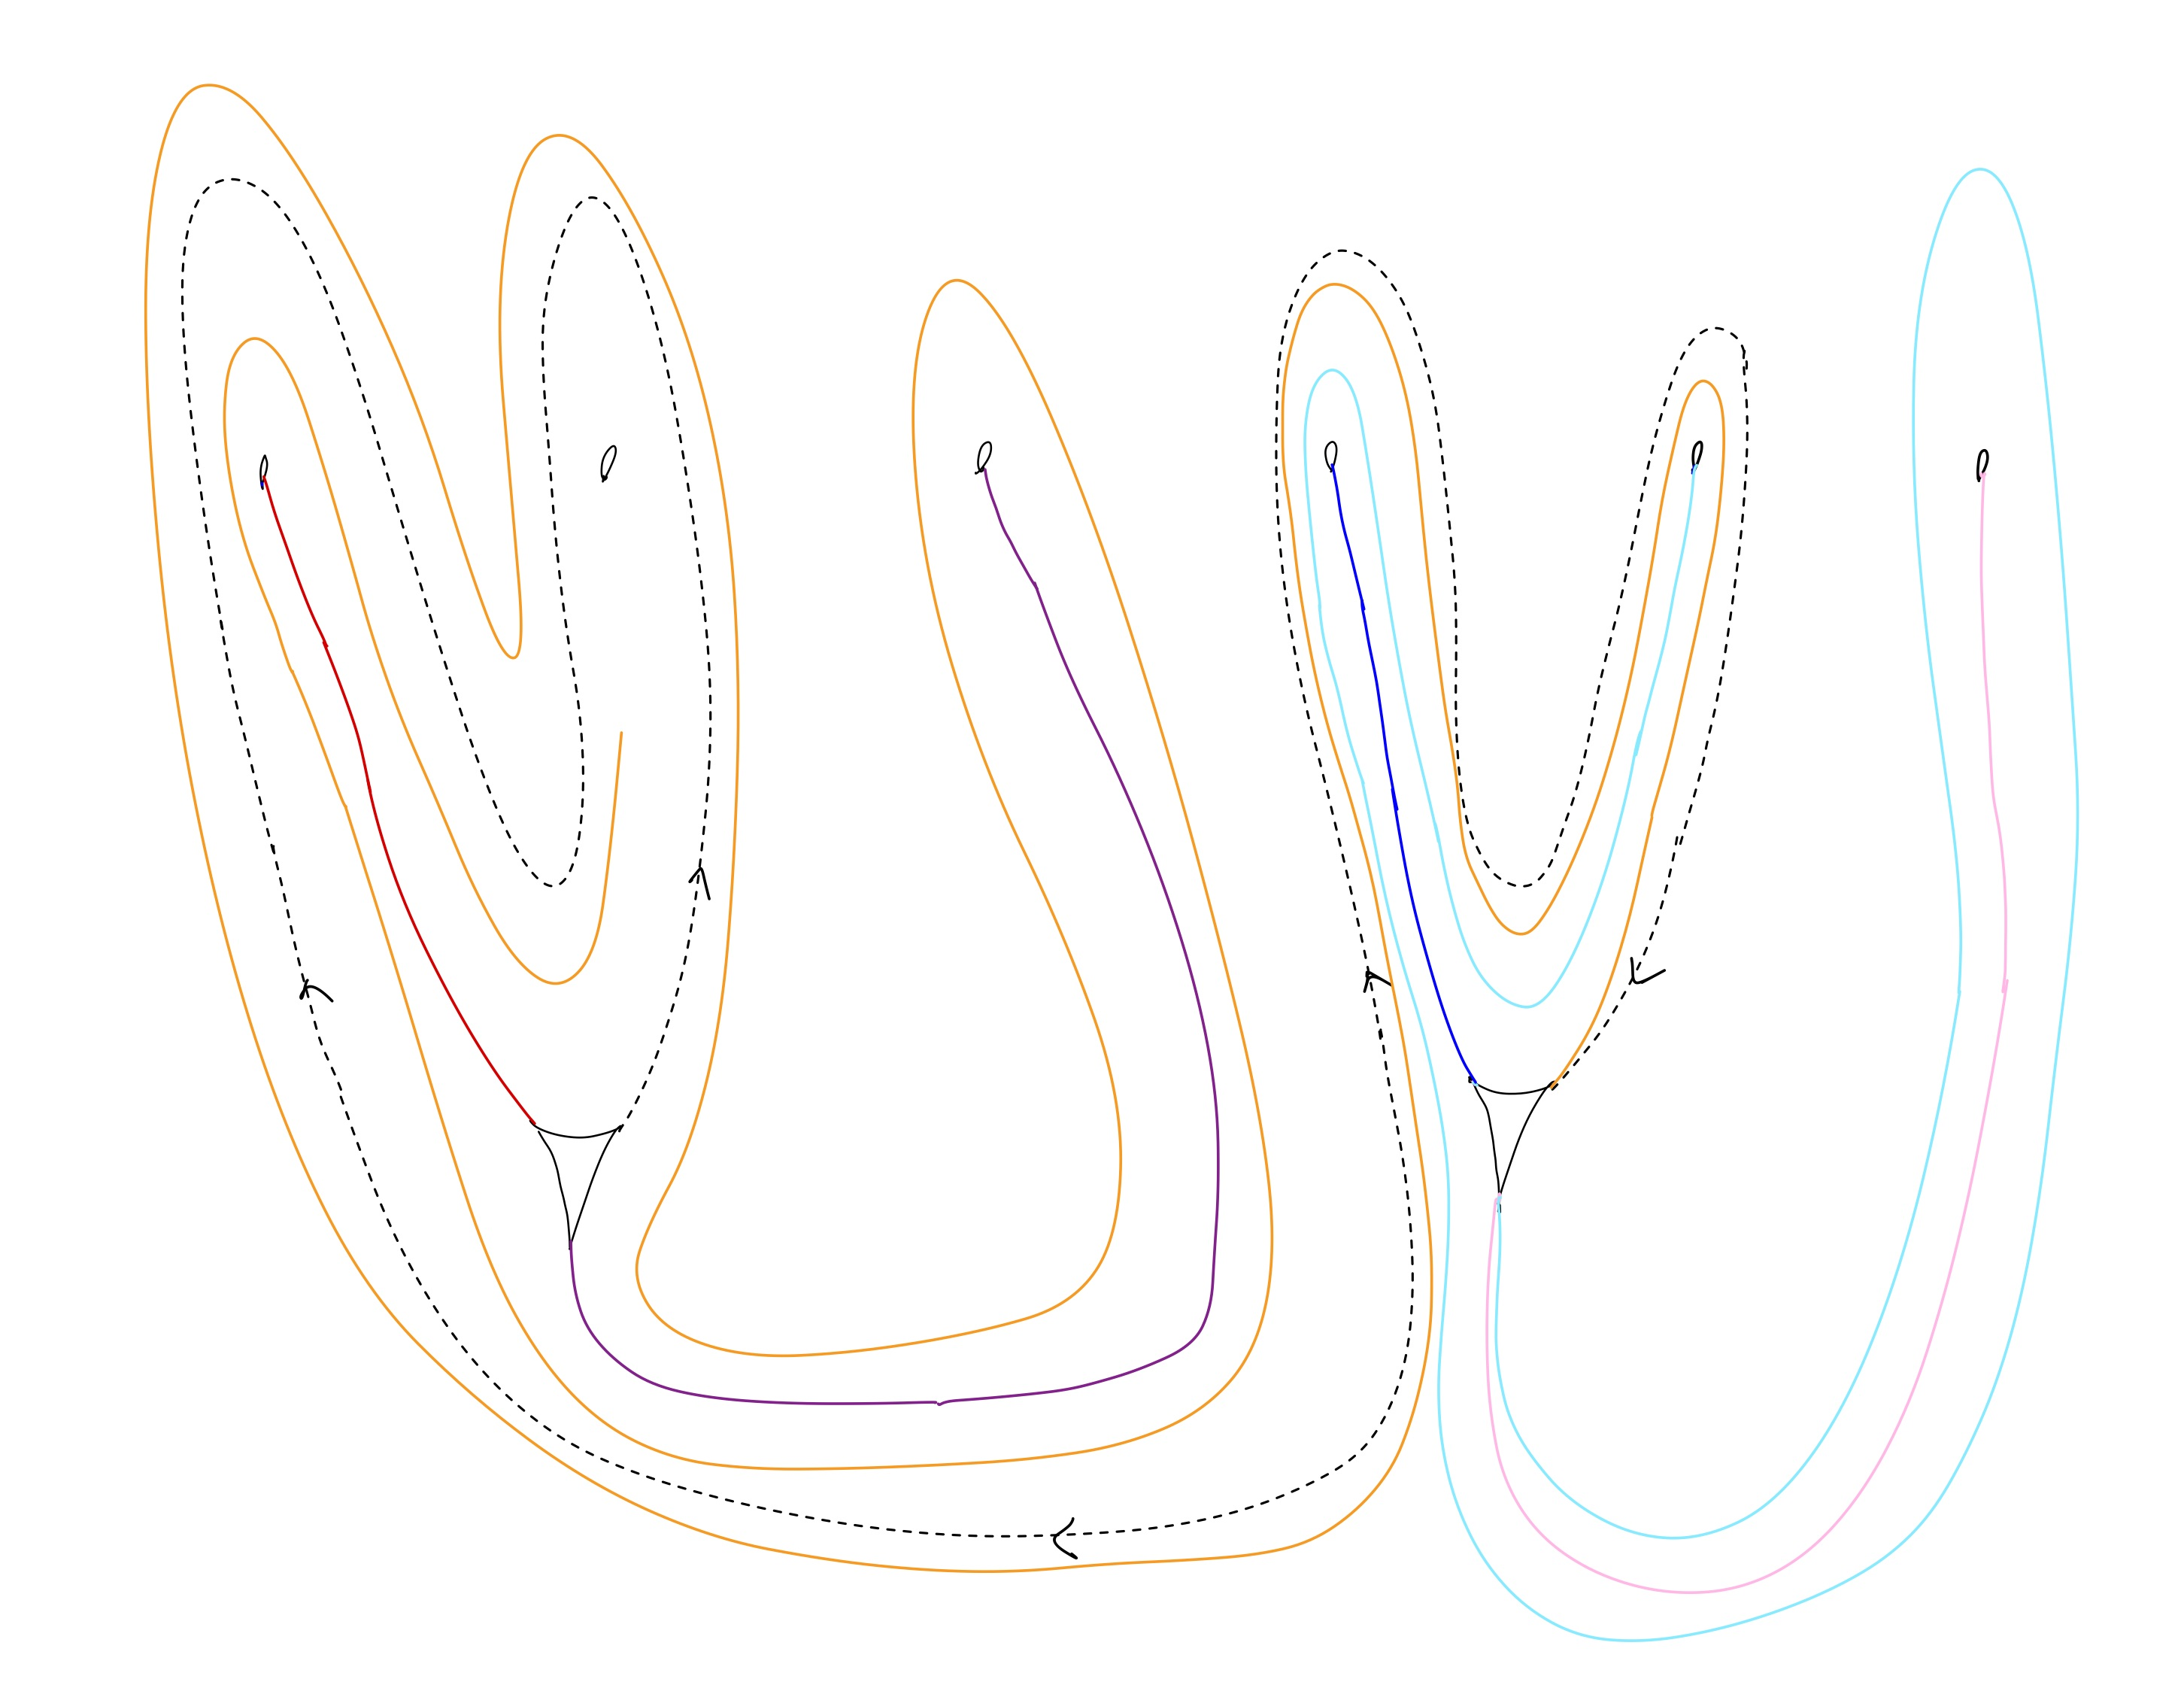
\includegraphics[width=\linewidth]{figures_case_analysis/track17_case_analysis/Flisky-13.jpg}
    \caption{Flisky13}
    \label{fig:Flisky13}
\end{figure}

\begin{figure}[ht]
    \centering
    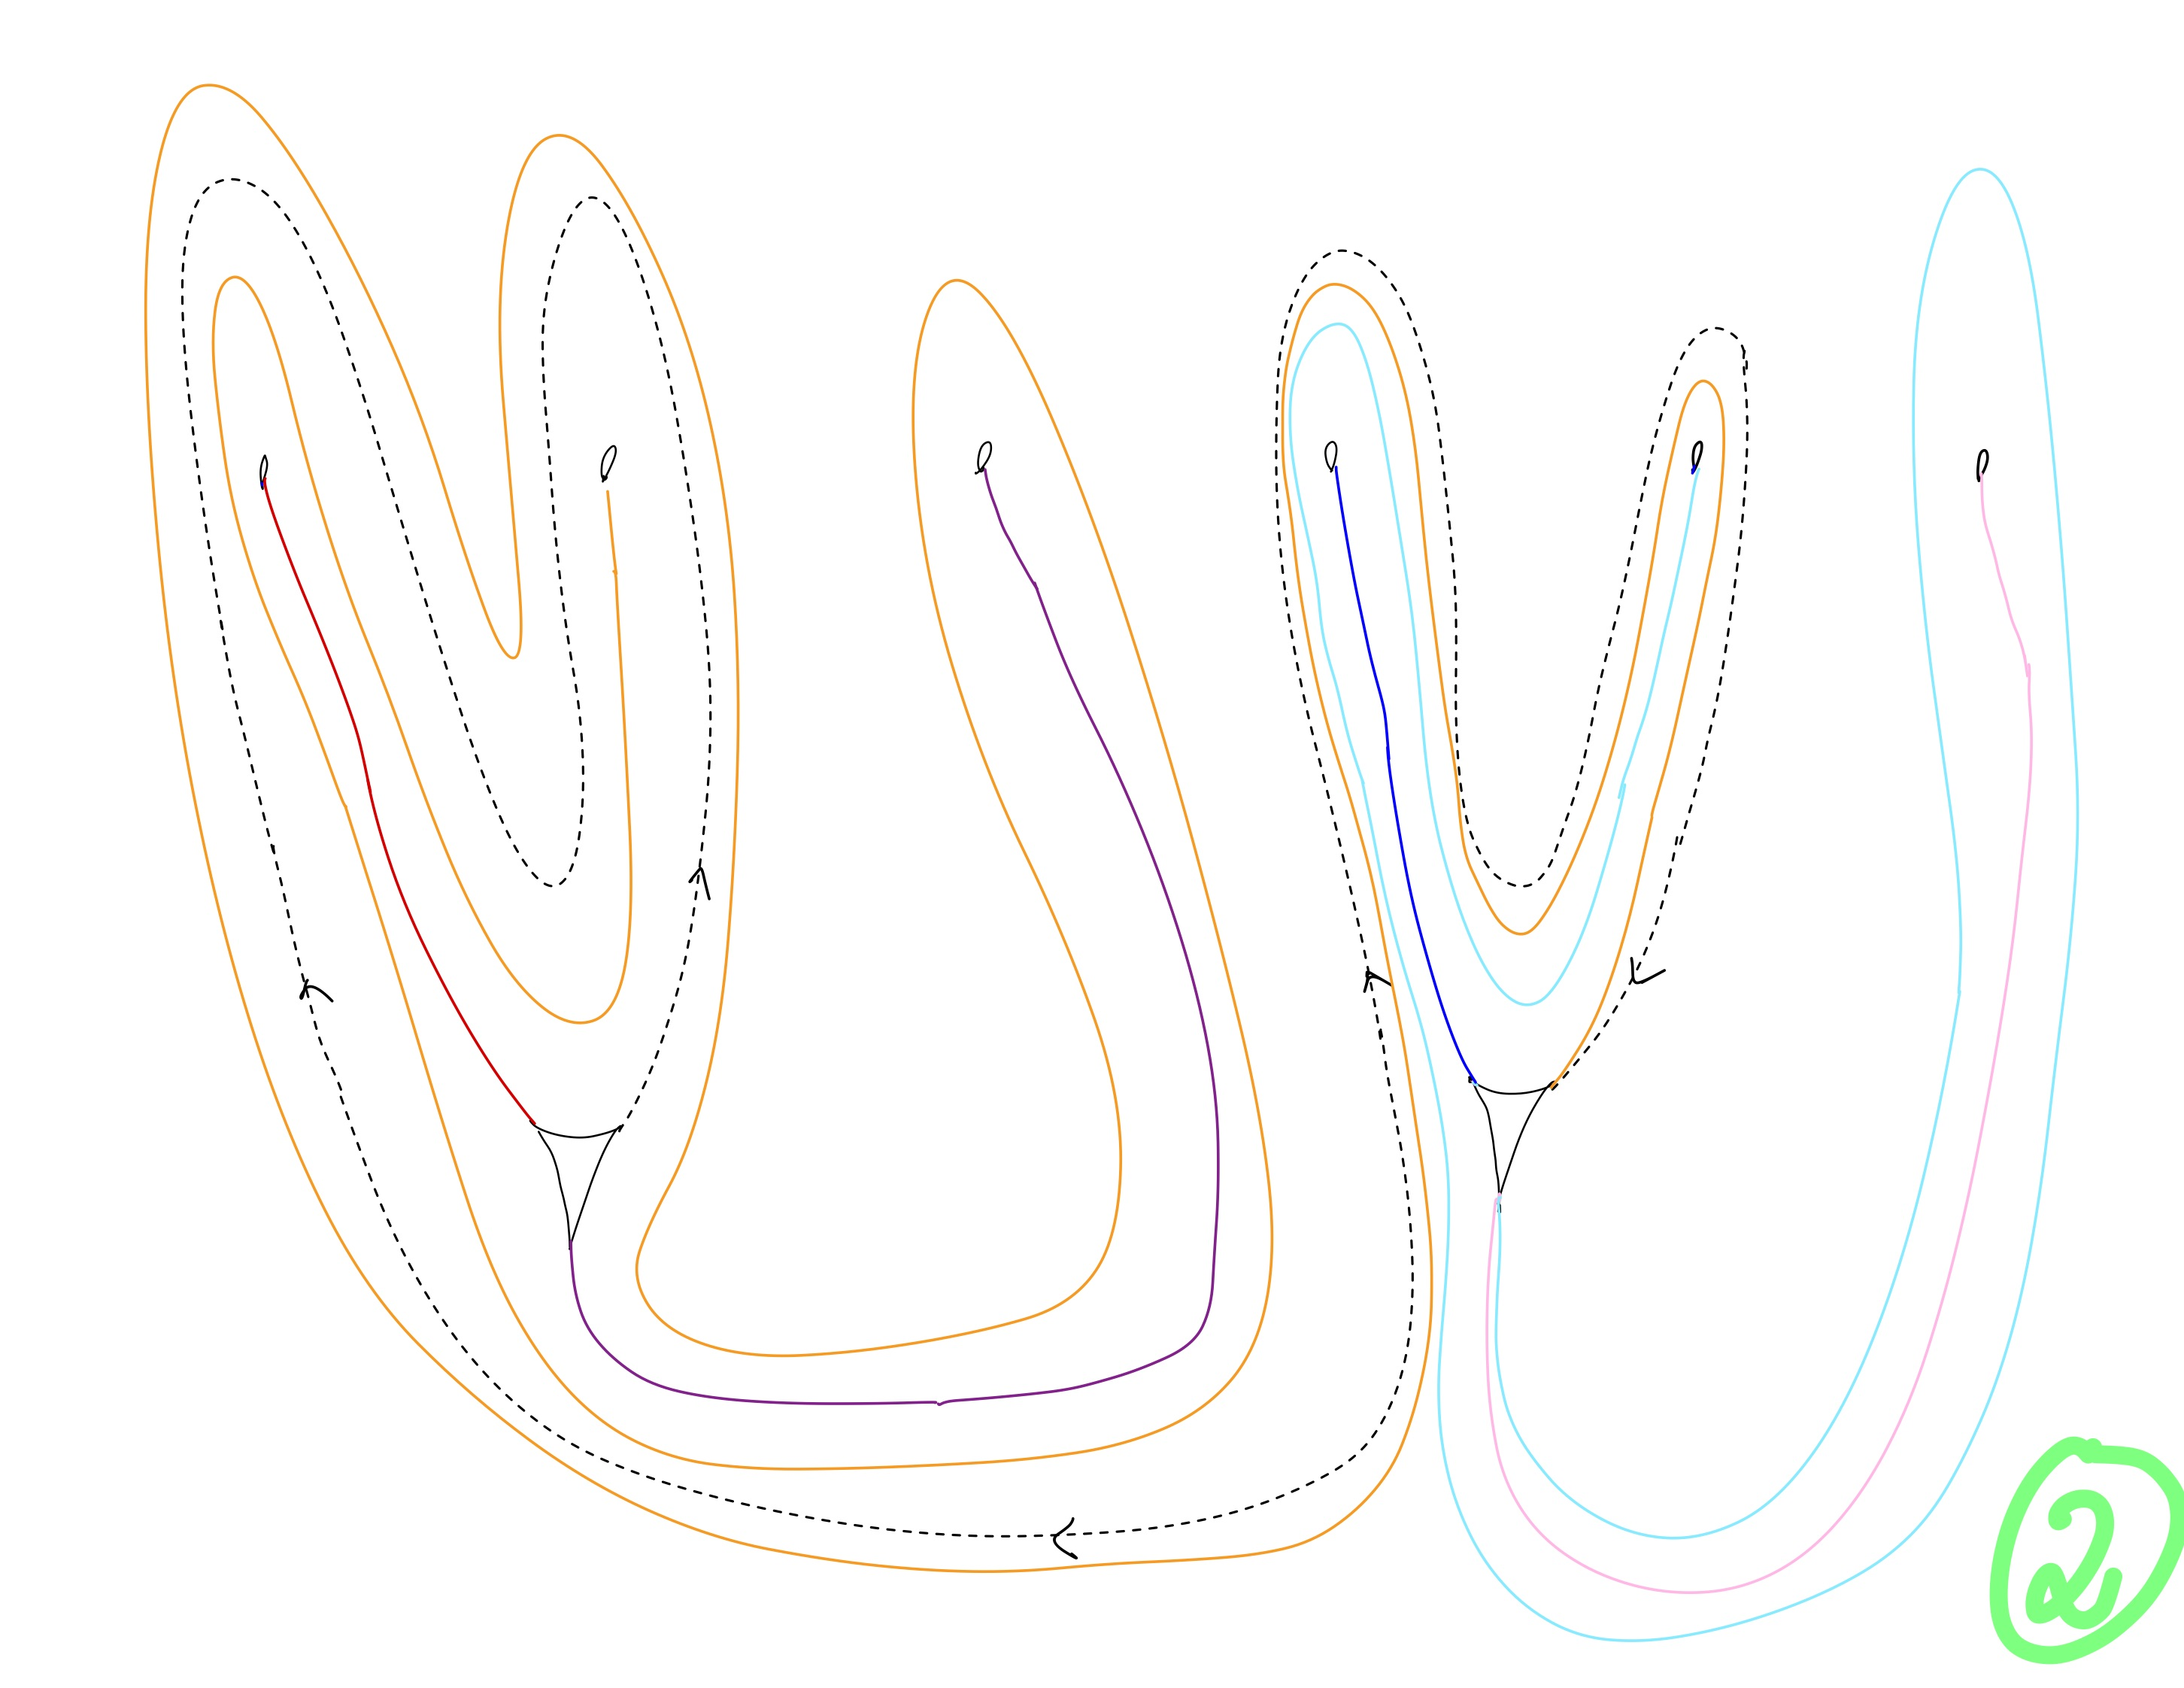
\includegraphics[width=\linewidth]{figures_case_analysis/track17_case_analysis/Flisky-14.jpg}
    \caption{Flisky14}
    \label{fig:Flisky14}
\end{figure}
\clearpage

\begin{figure}[ht]
    \centering
    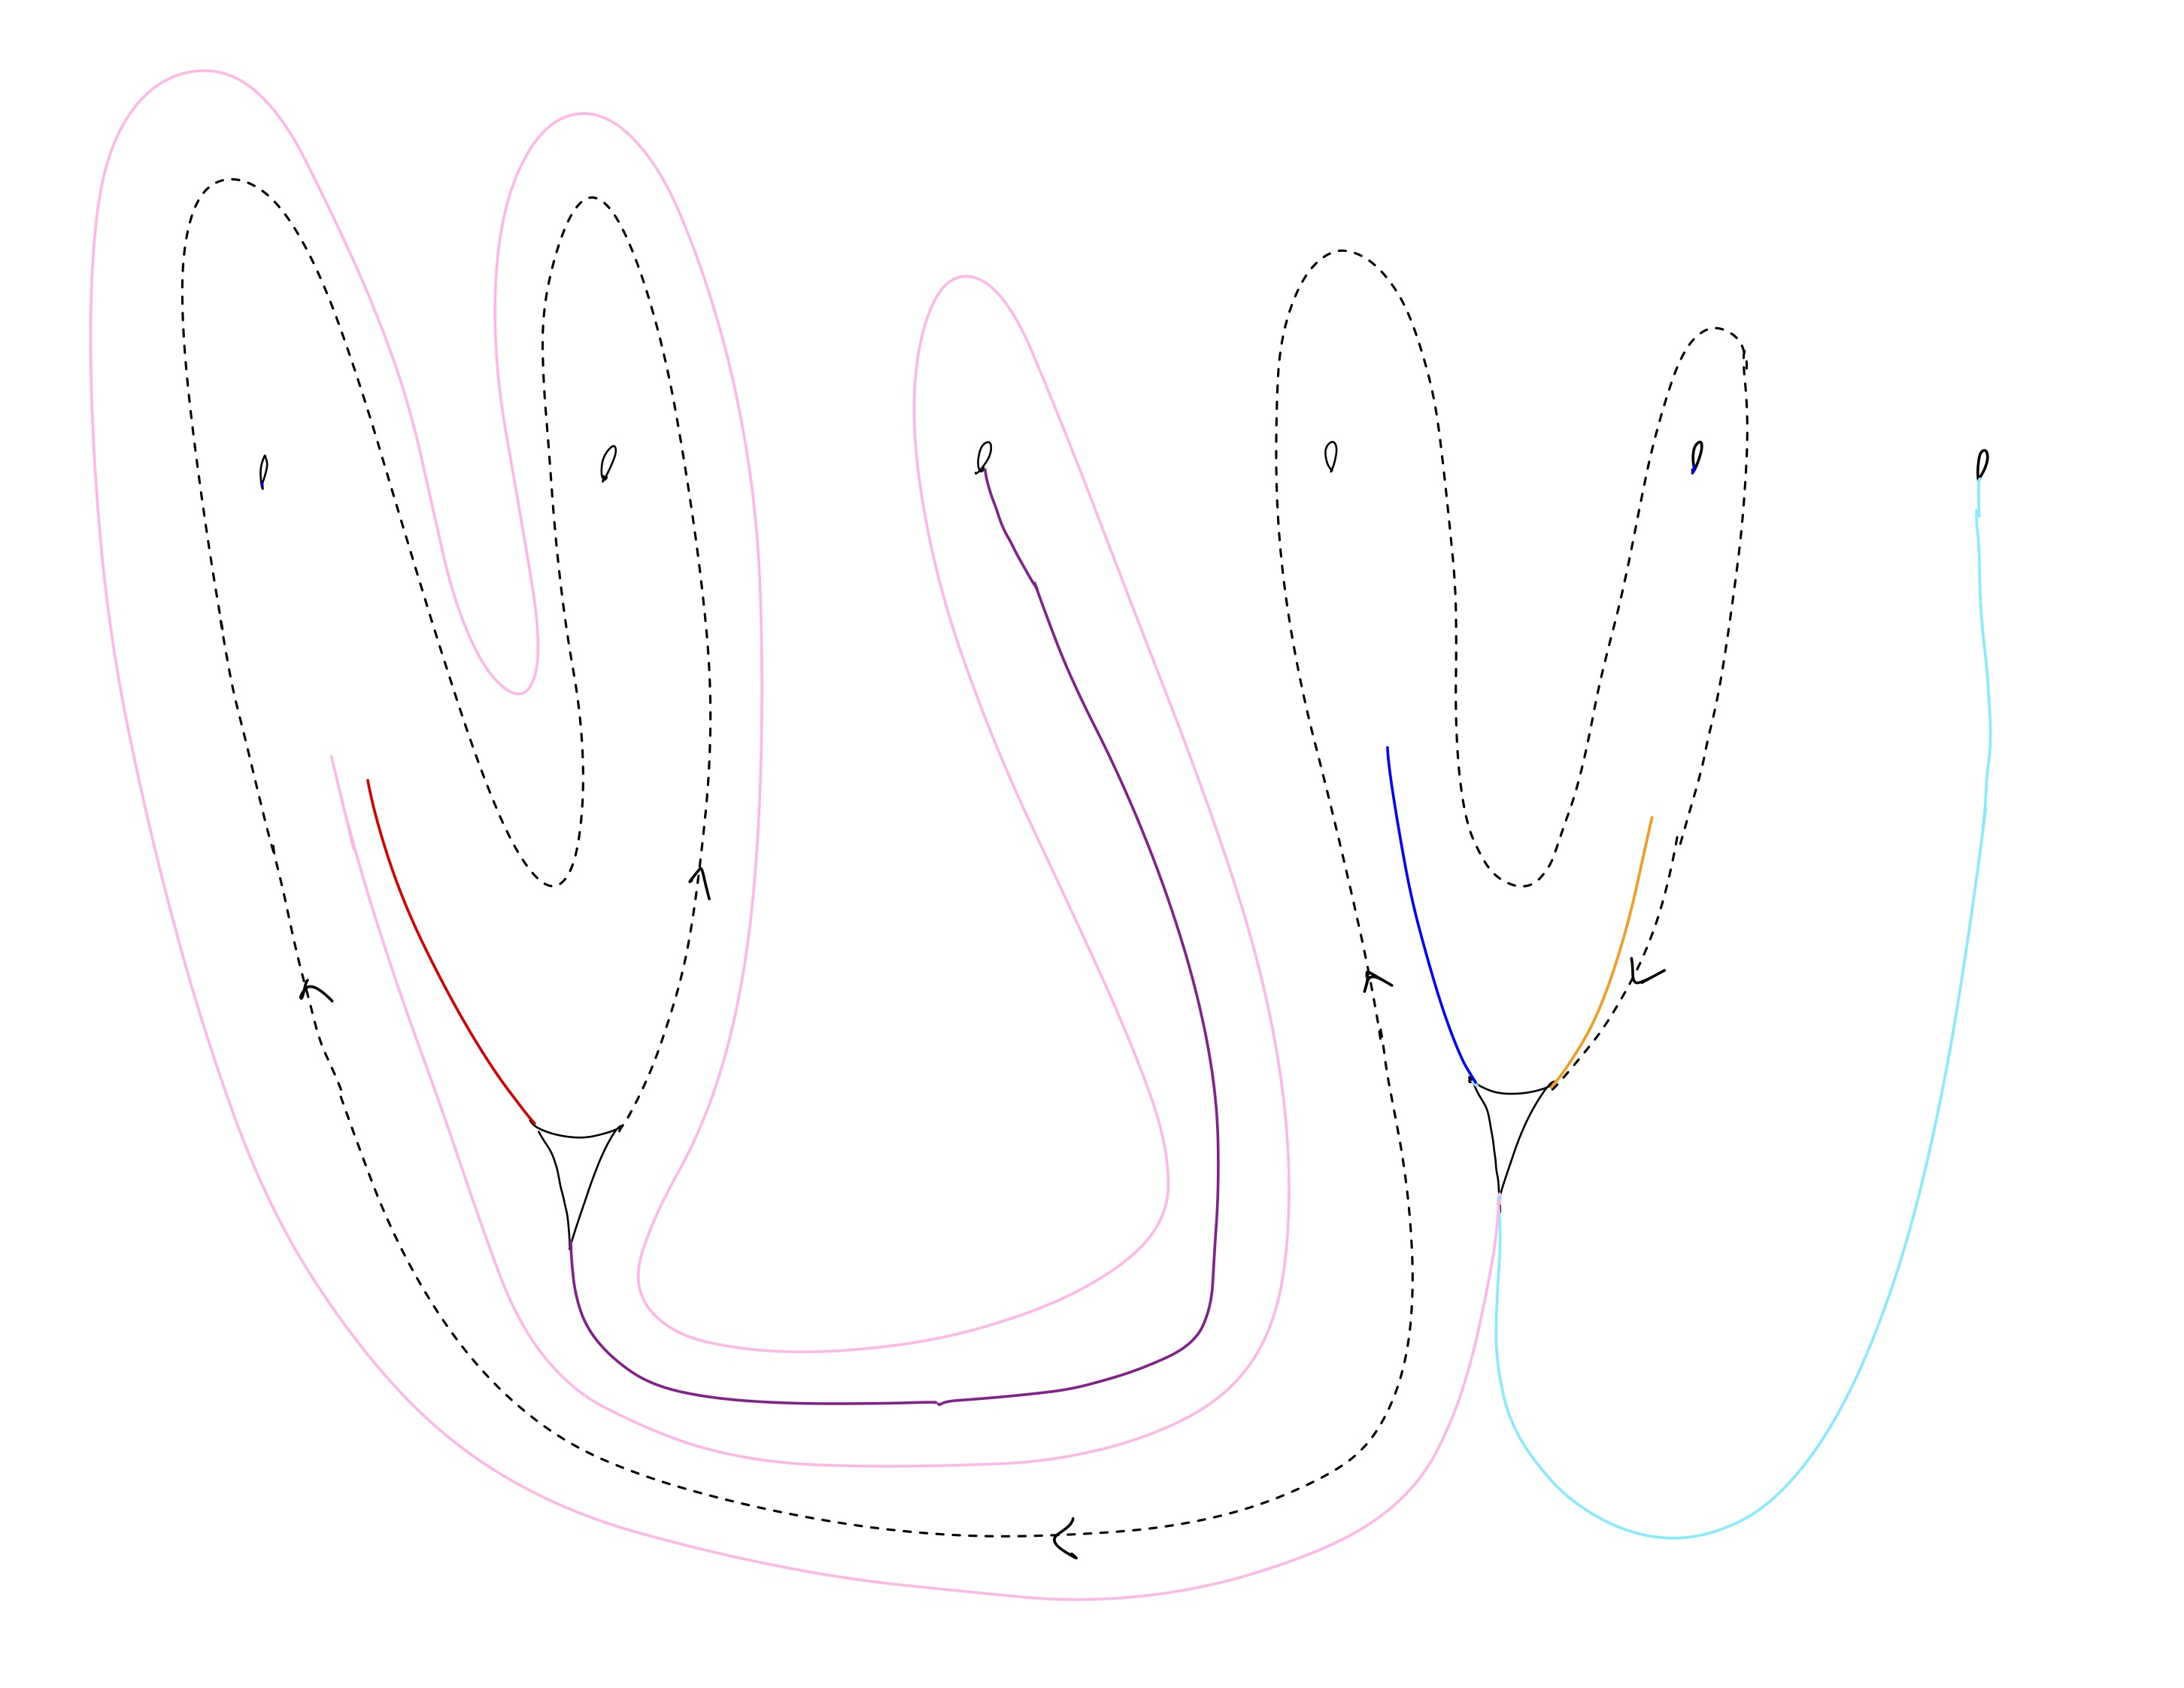
\includegraphics[width=\linewidth]{figures_case_analysis/track17_case_analysis/Wanion-1.jpg}
    \caption{Wanion1}
    \label{fig:Wanion1}
\end{figure}

\begin{figure}[ht]
    \centering
    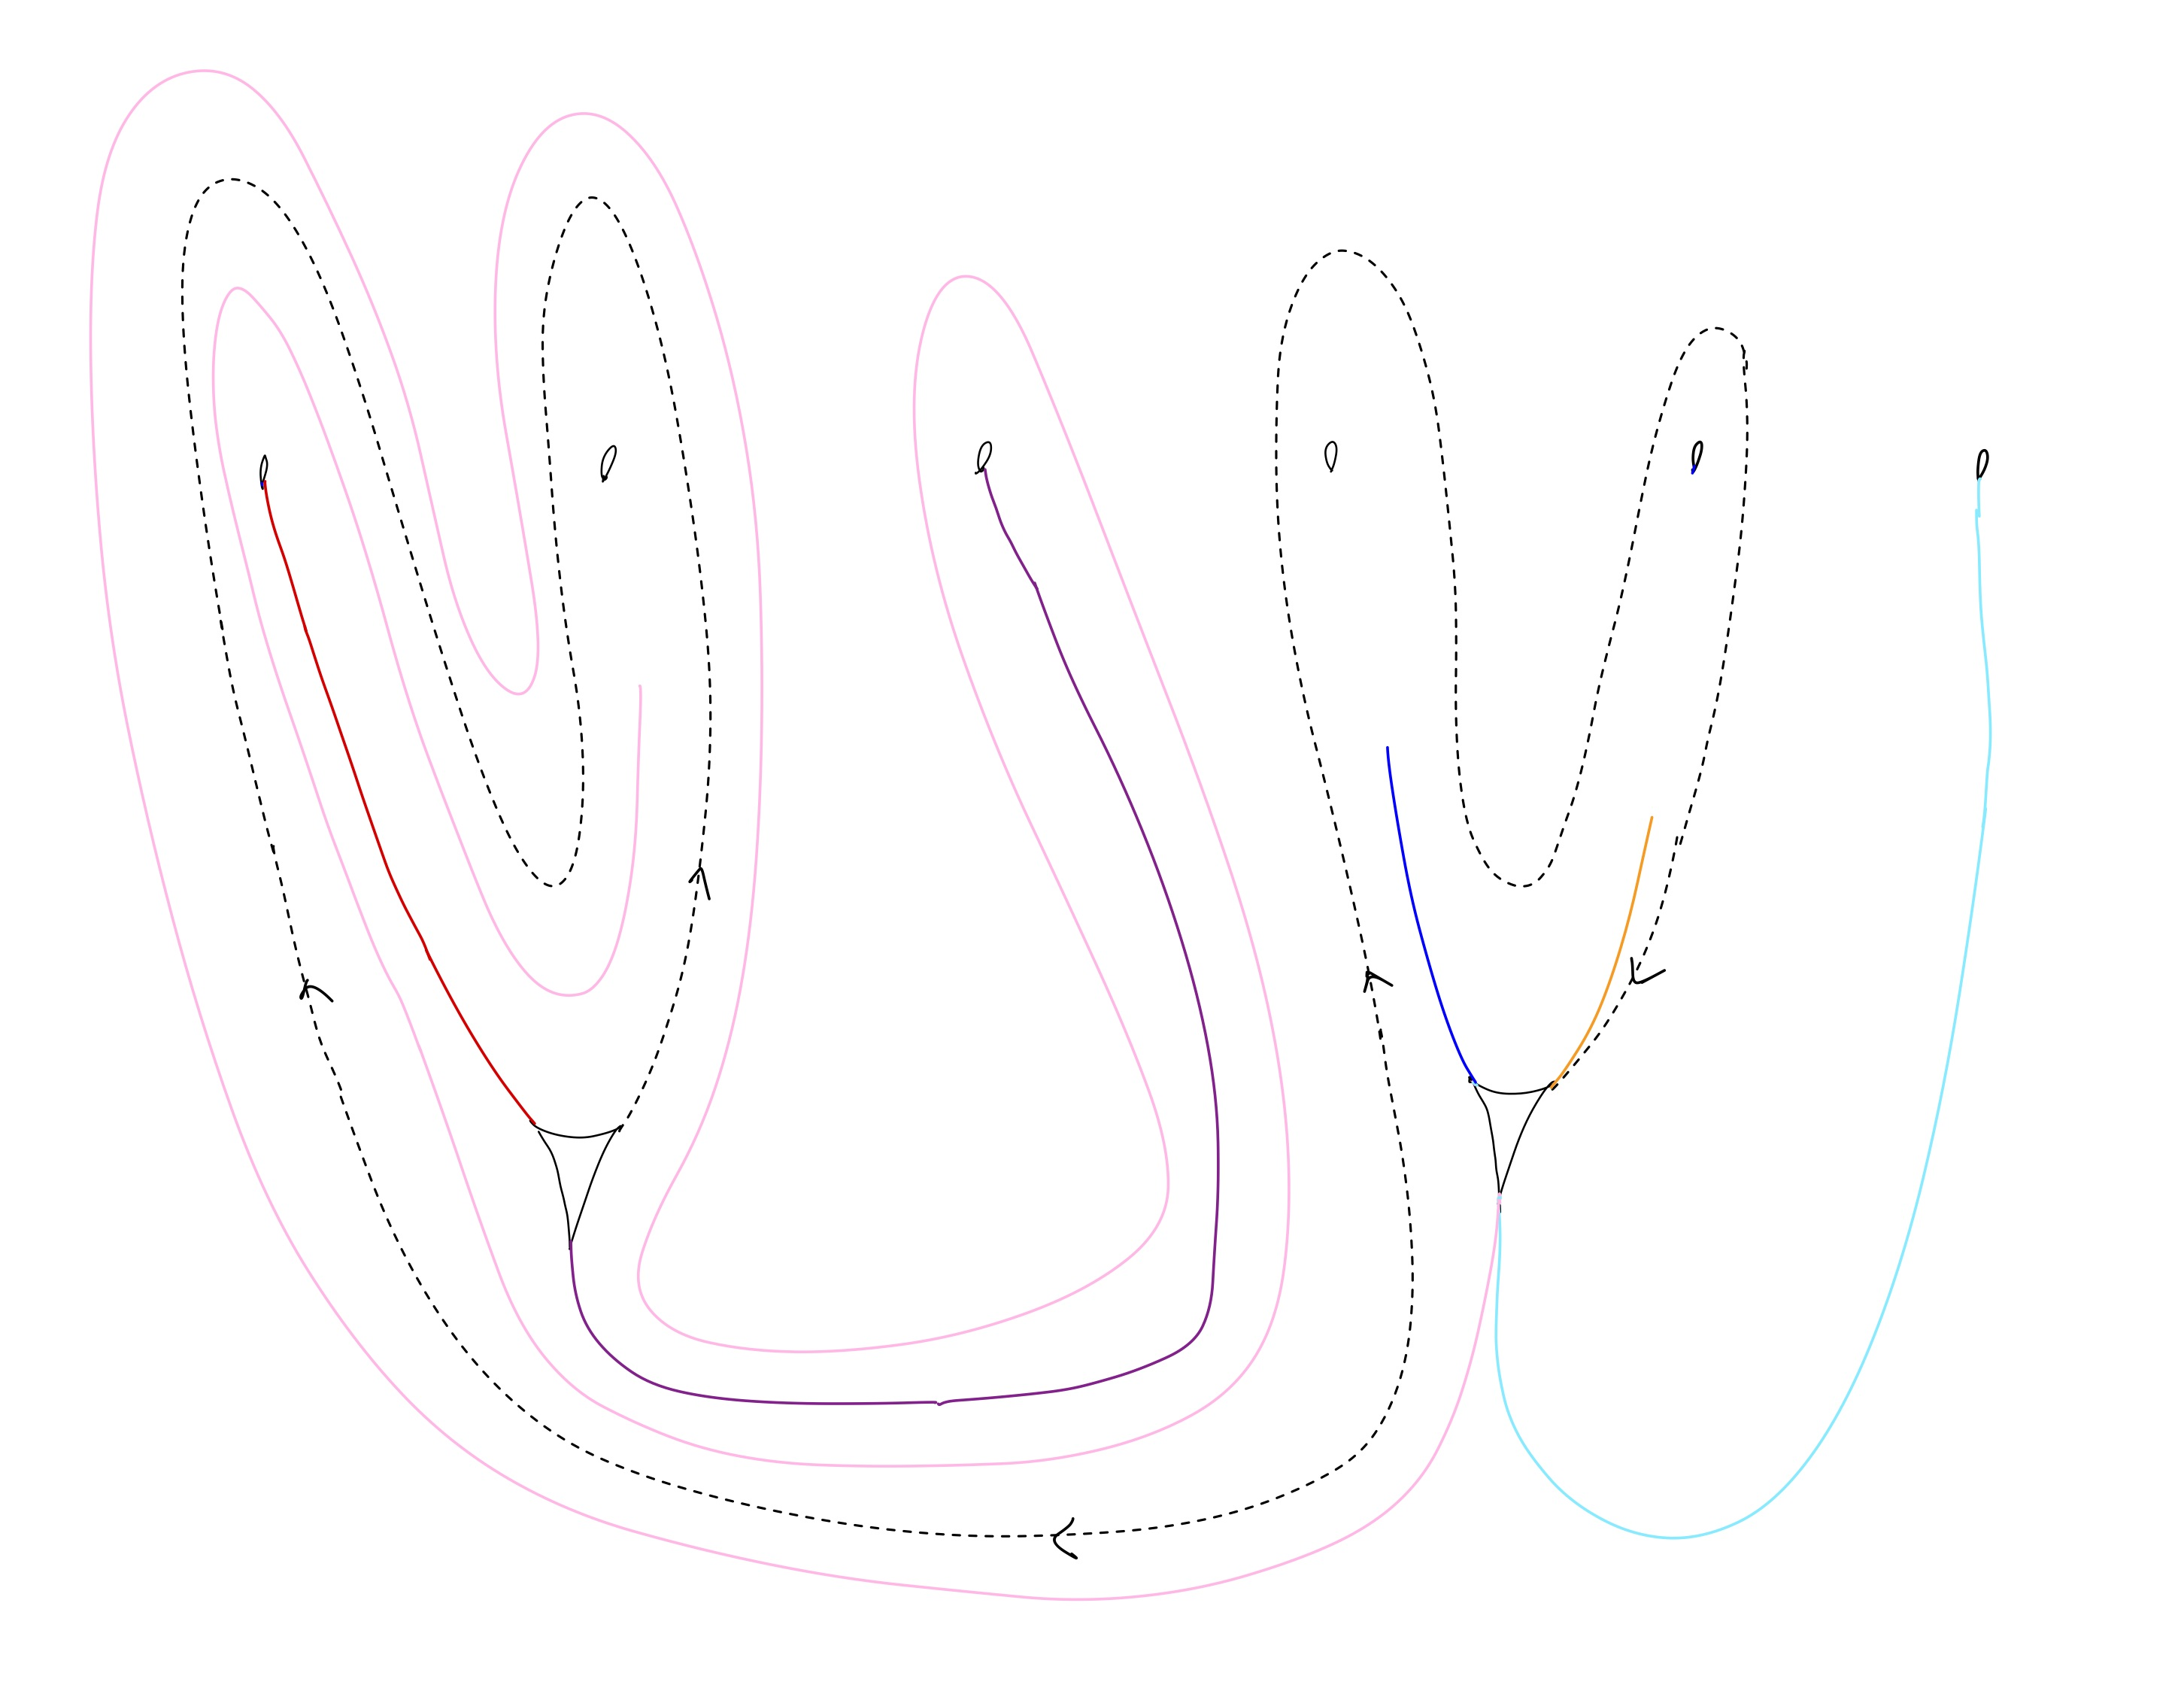
\includegraphics[width=\linewidth]{figures_case_analysis/track17_case_analysis/Wanion-2.jpg}
    \caption{Wanion2}
    \label{fig:Wanion2}
\end{figure}

\begin{figure}[ht]
    \centering
    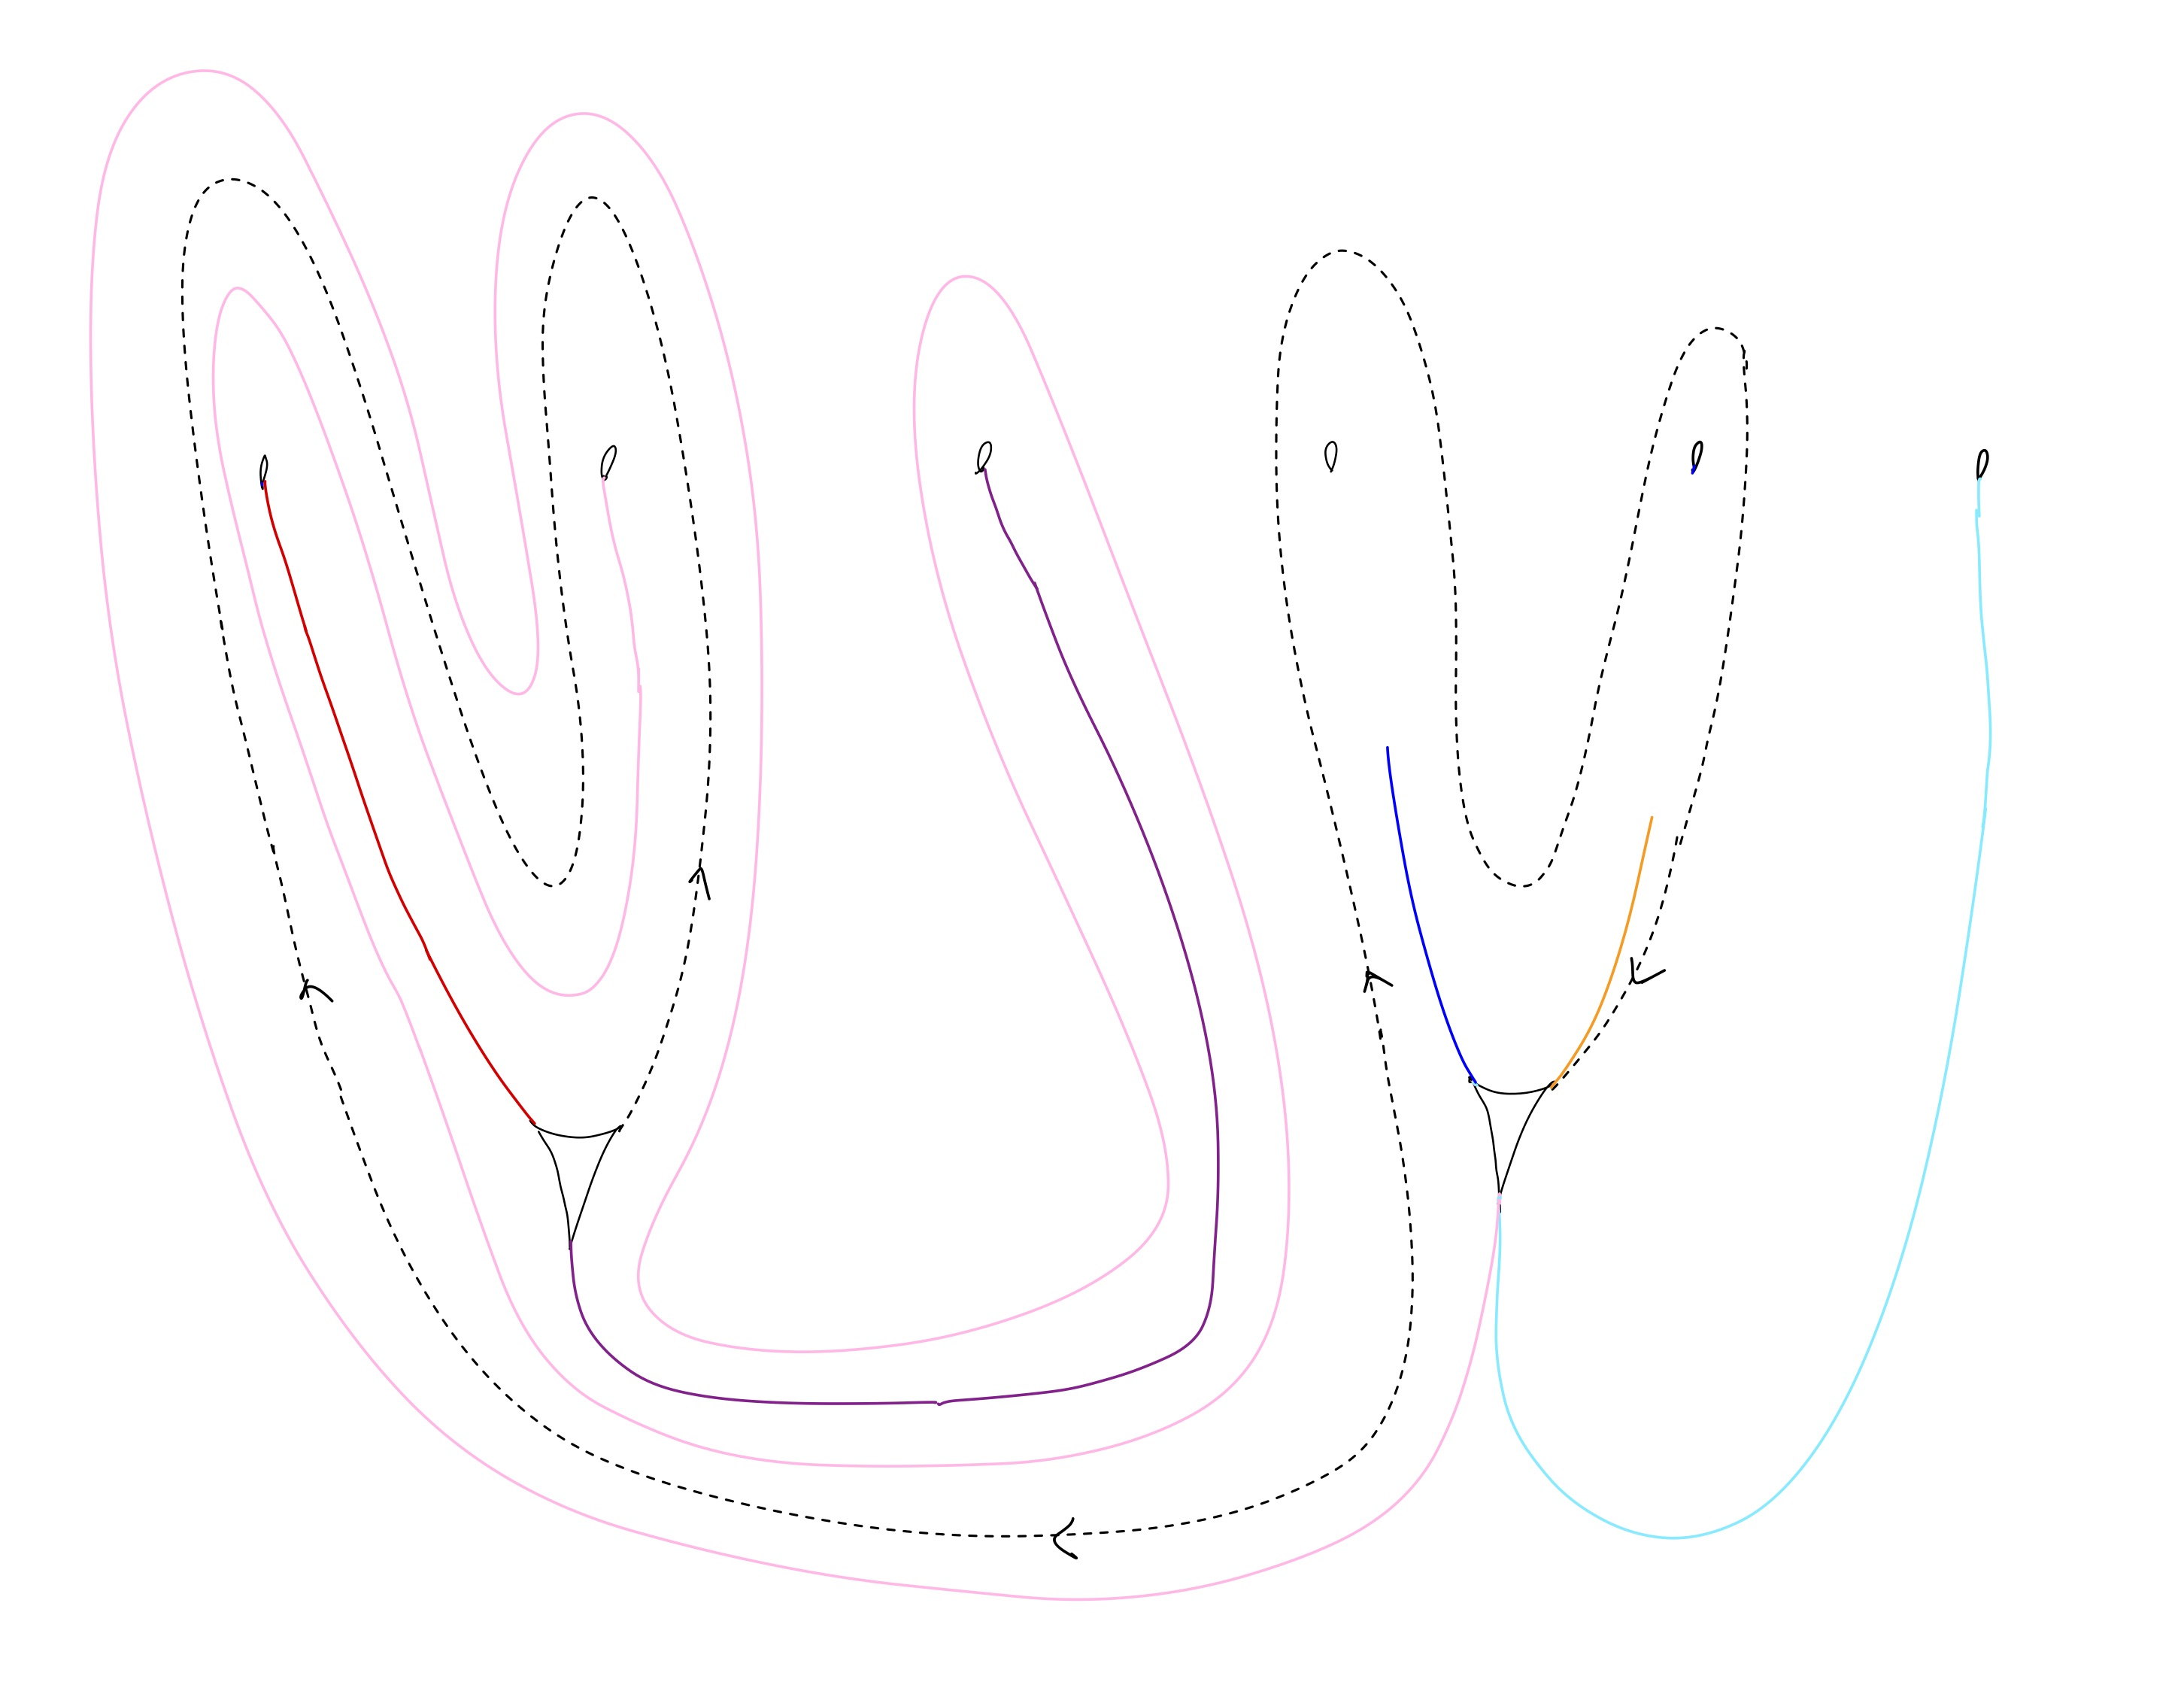
\includegraphics[width=\linewidth]{figures_case_analysis/track17_case_analysis/Wanion-3.jpg}
    \caption{Wanion3}
    \label{fig:Wanion3}
\end{figure}

\begin{figure}[ht]
    \centering
    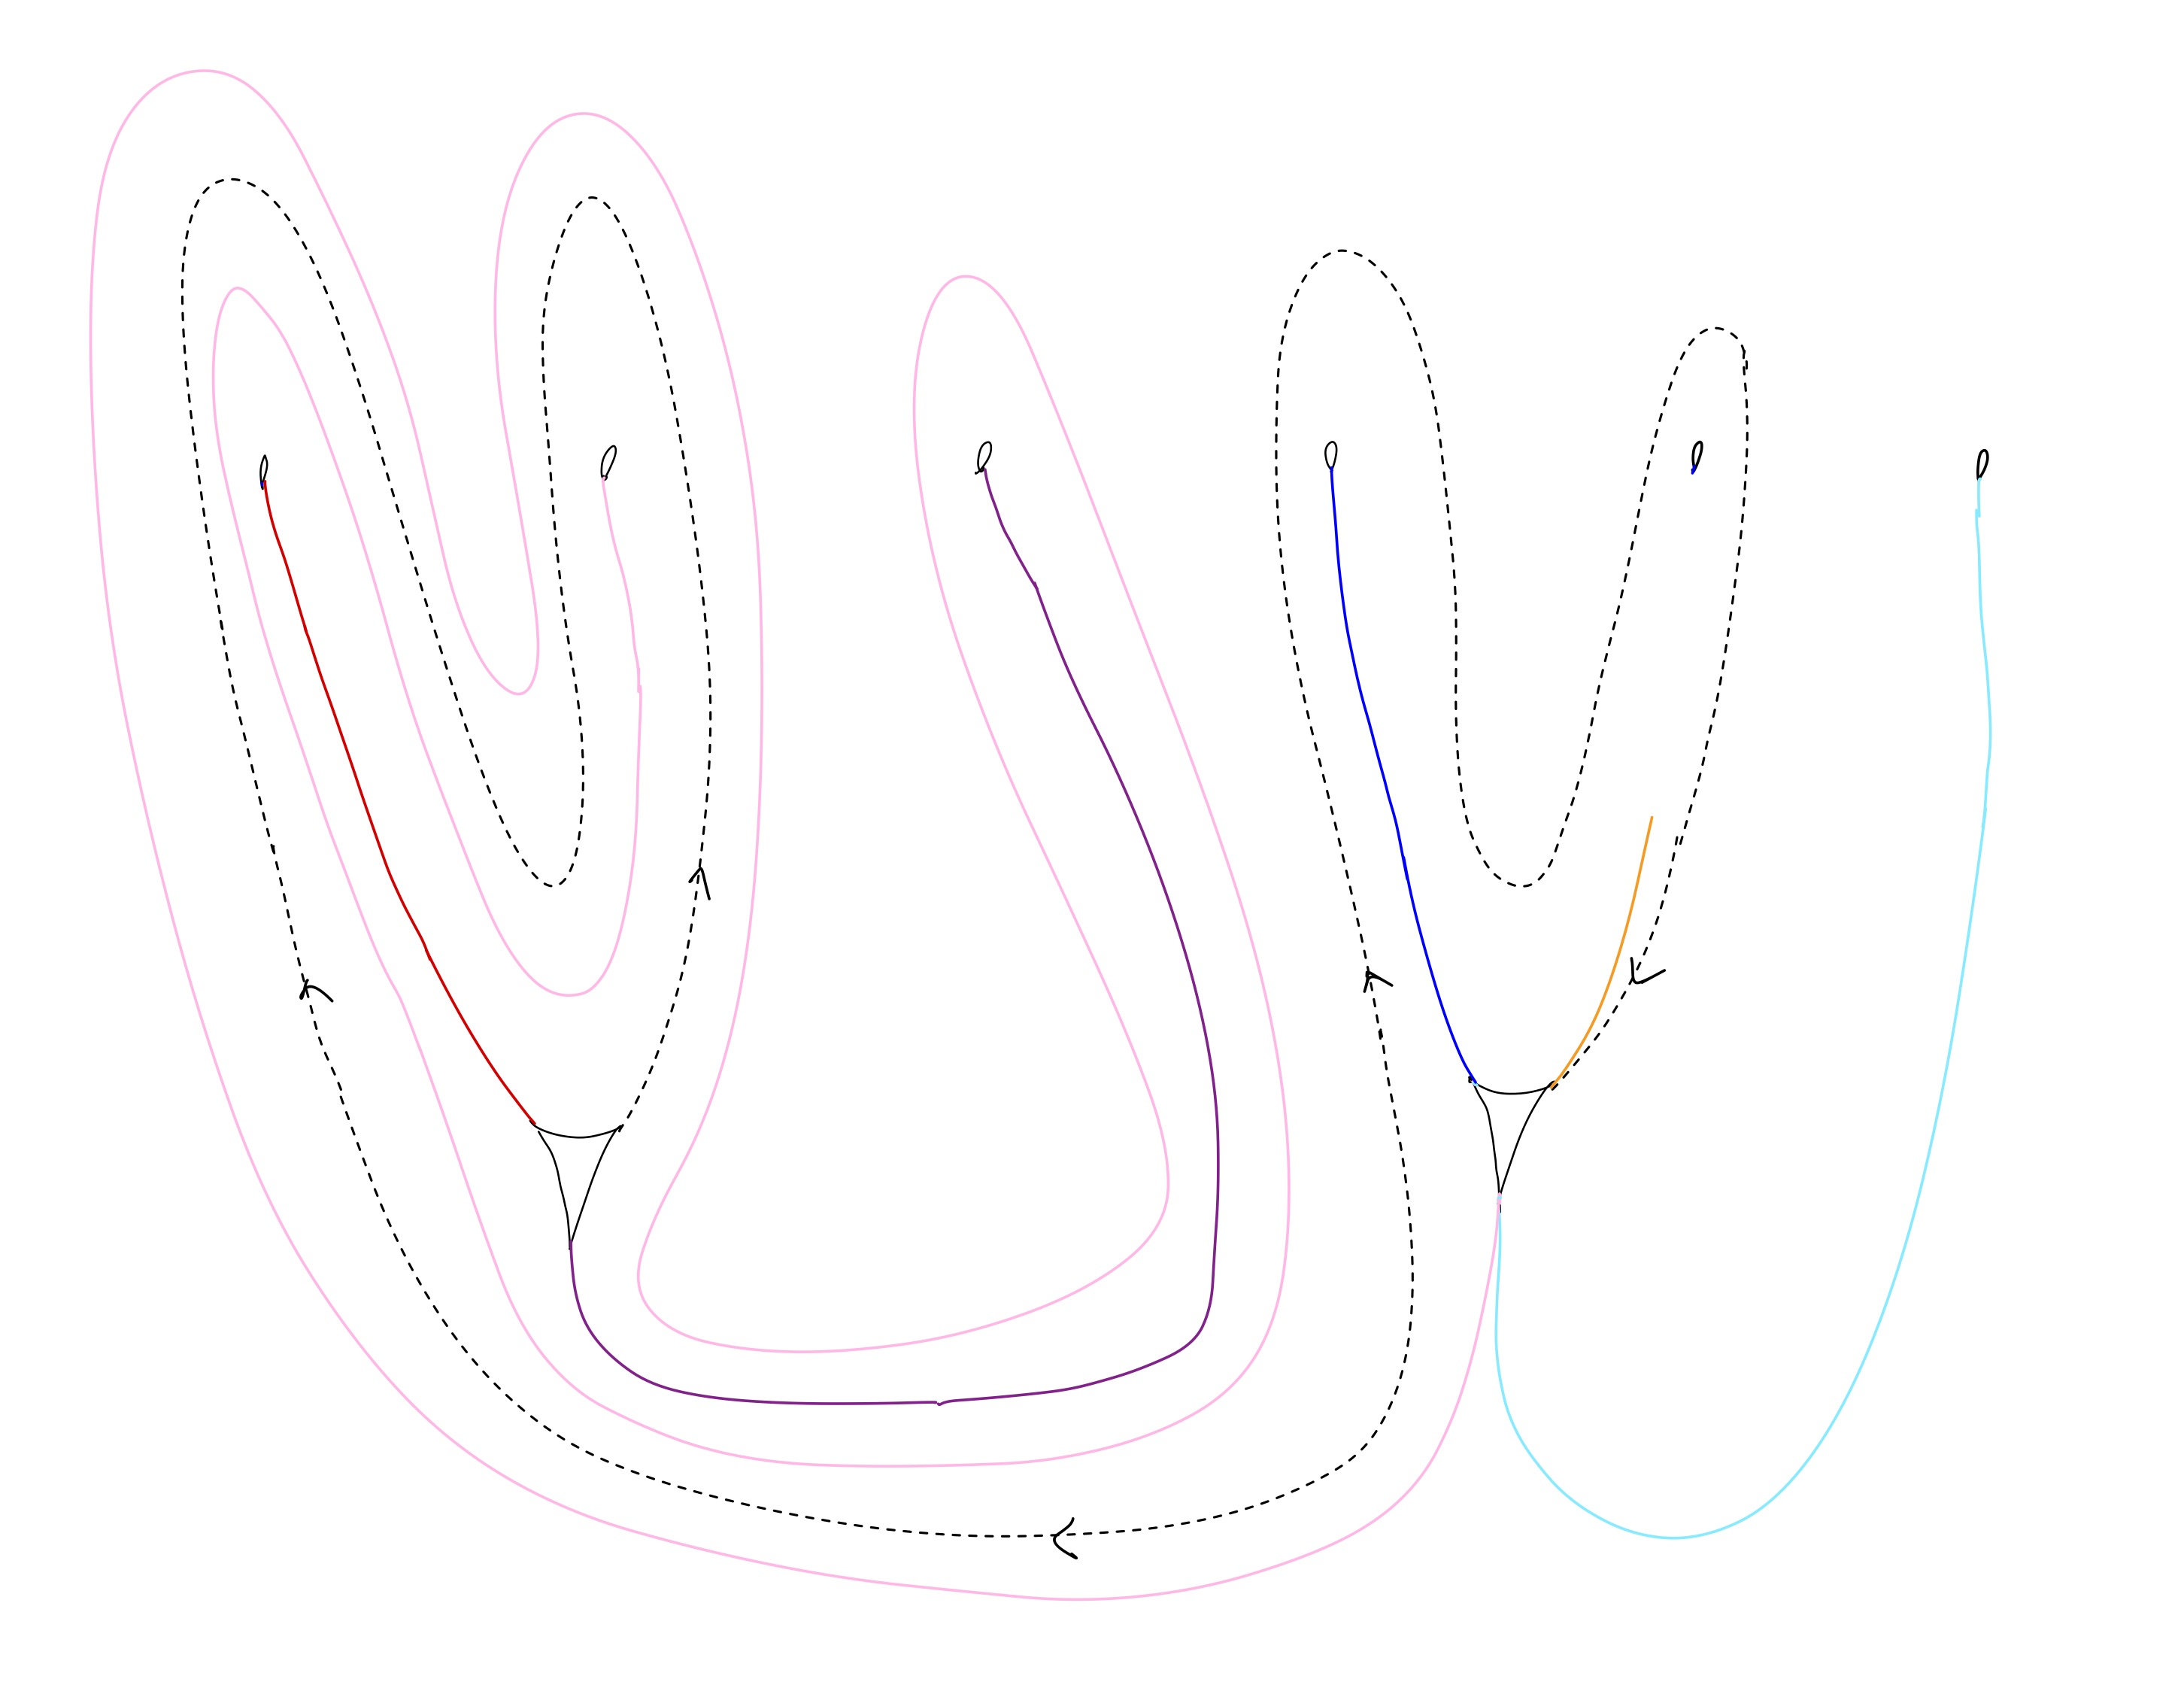
\includegraphics[width=\linewidth]{figures_case_analysis/track17_case_analysis/Wanion-4.jpg}
    \caption{Wanion4}
    \label{fig:Wanion4}
\end{figure}

\begin{figure}[ht]
    \centering
    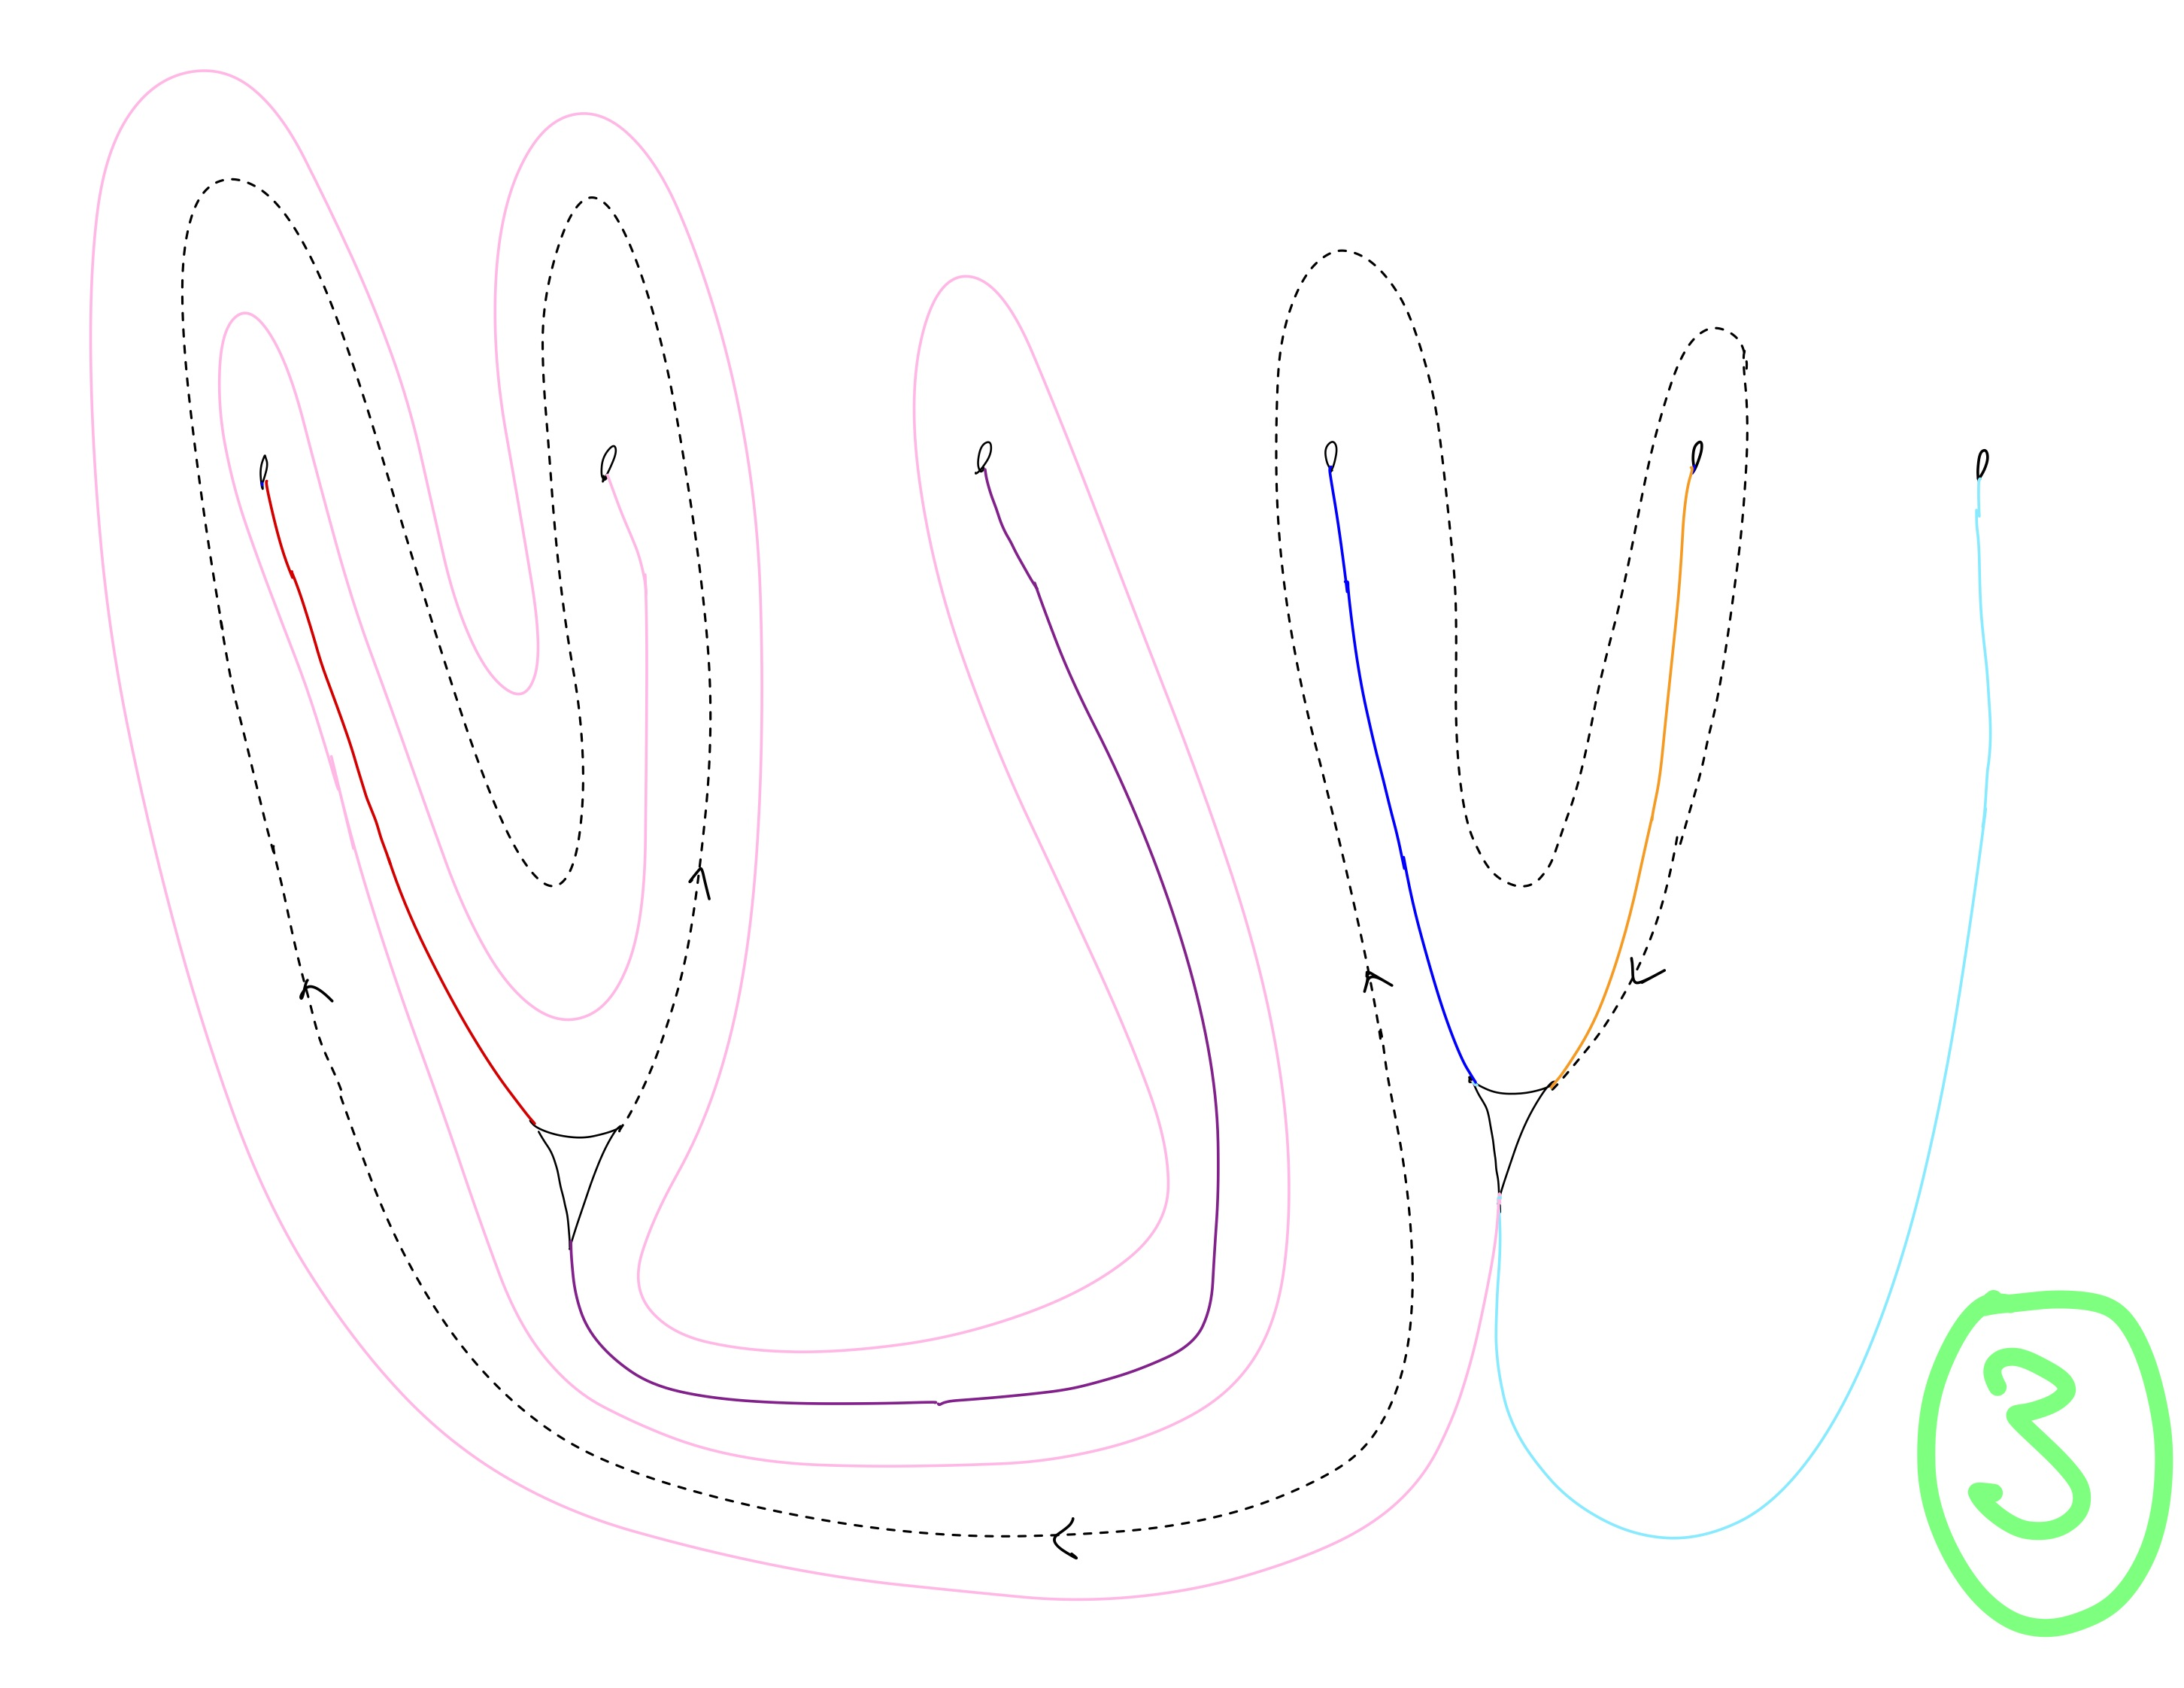
\includegraphics[width=\linewidth]{figures_case_analysis/track17_case_analysis/Wanion-5.jpg}
    \caption{Wanion5}
    \label{fig:Wanion5}
\end{figure}
\clearpage

\begin{figure}[ht]
    \centering
    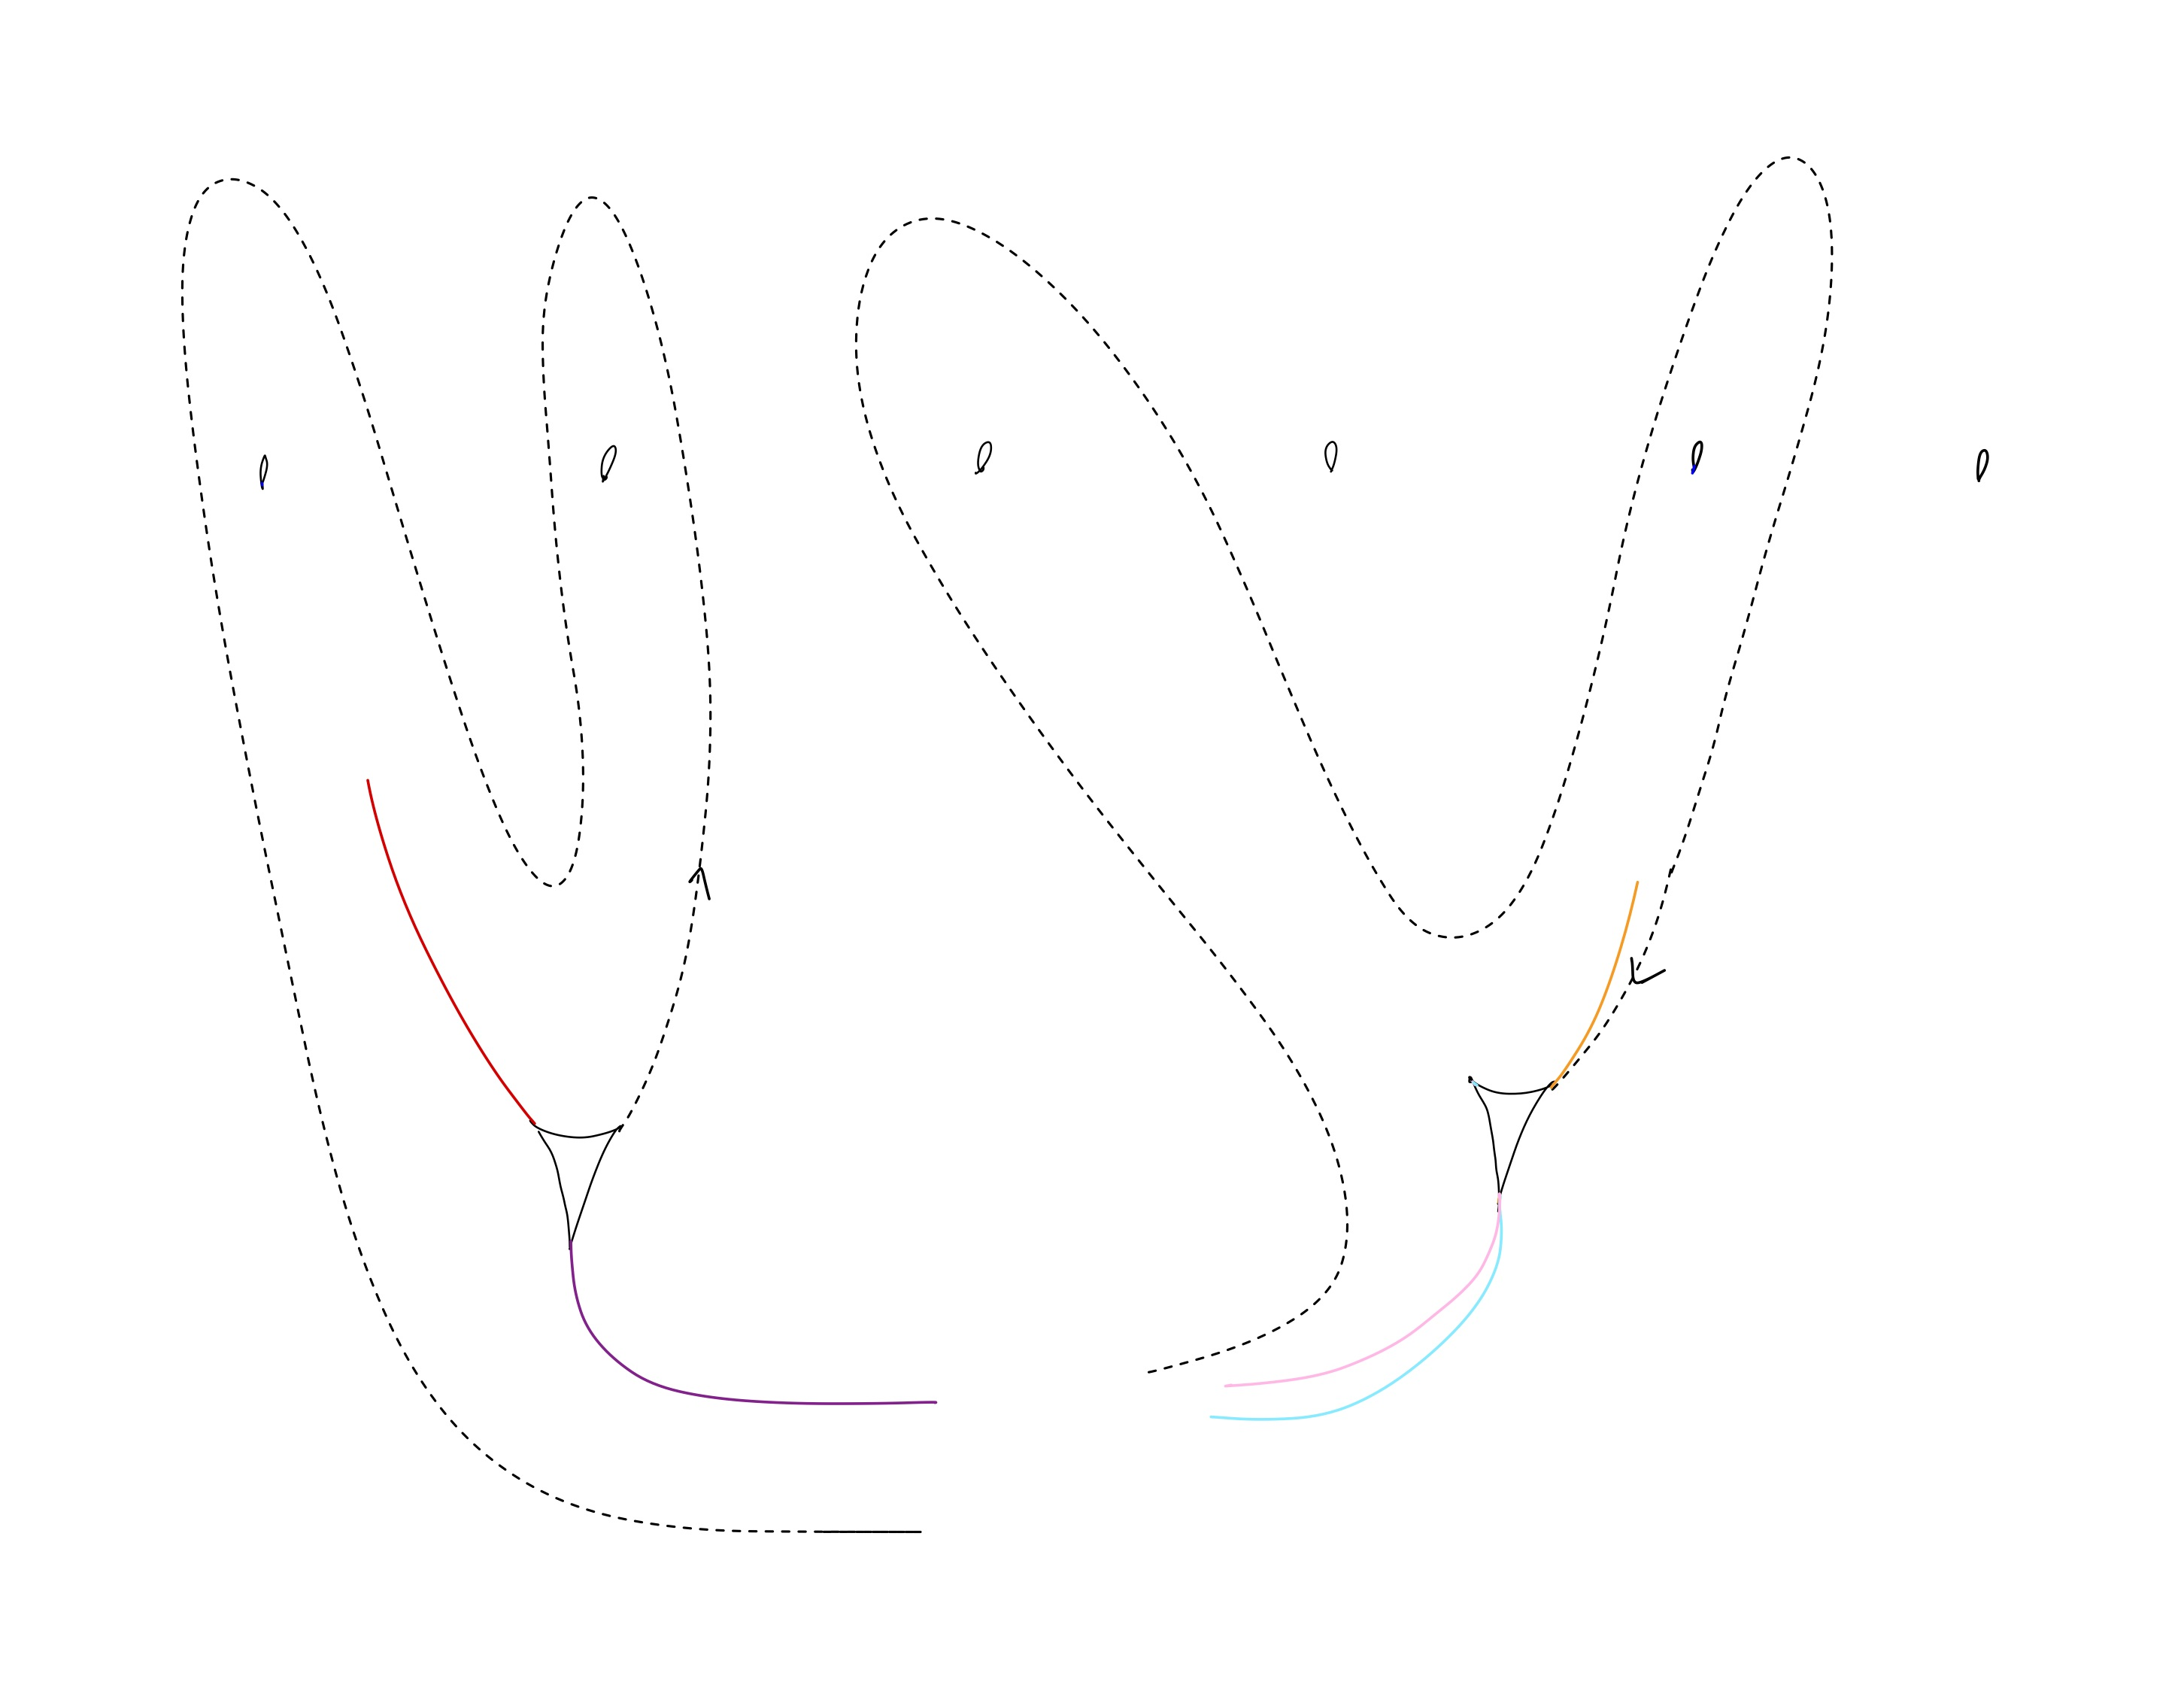
\includegraphics[width=\linewidth]{figures_case_analysis/track17_case_analysis/Blet-1.jpg}
    \caption{Blet1}
    \label{fig:Blet1}
\end{figure}

\begin{figure}[ht]
    \centering
    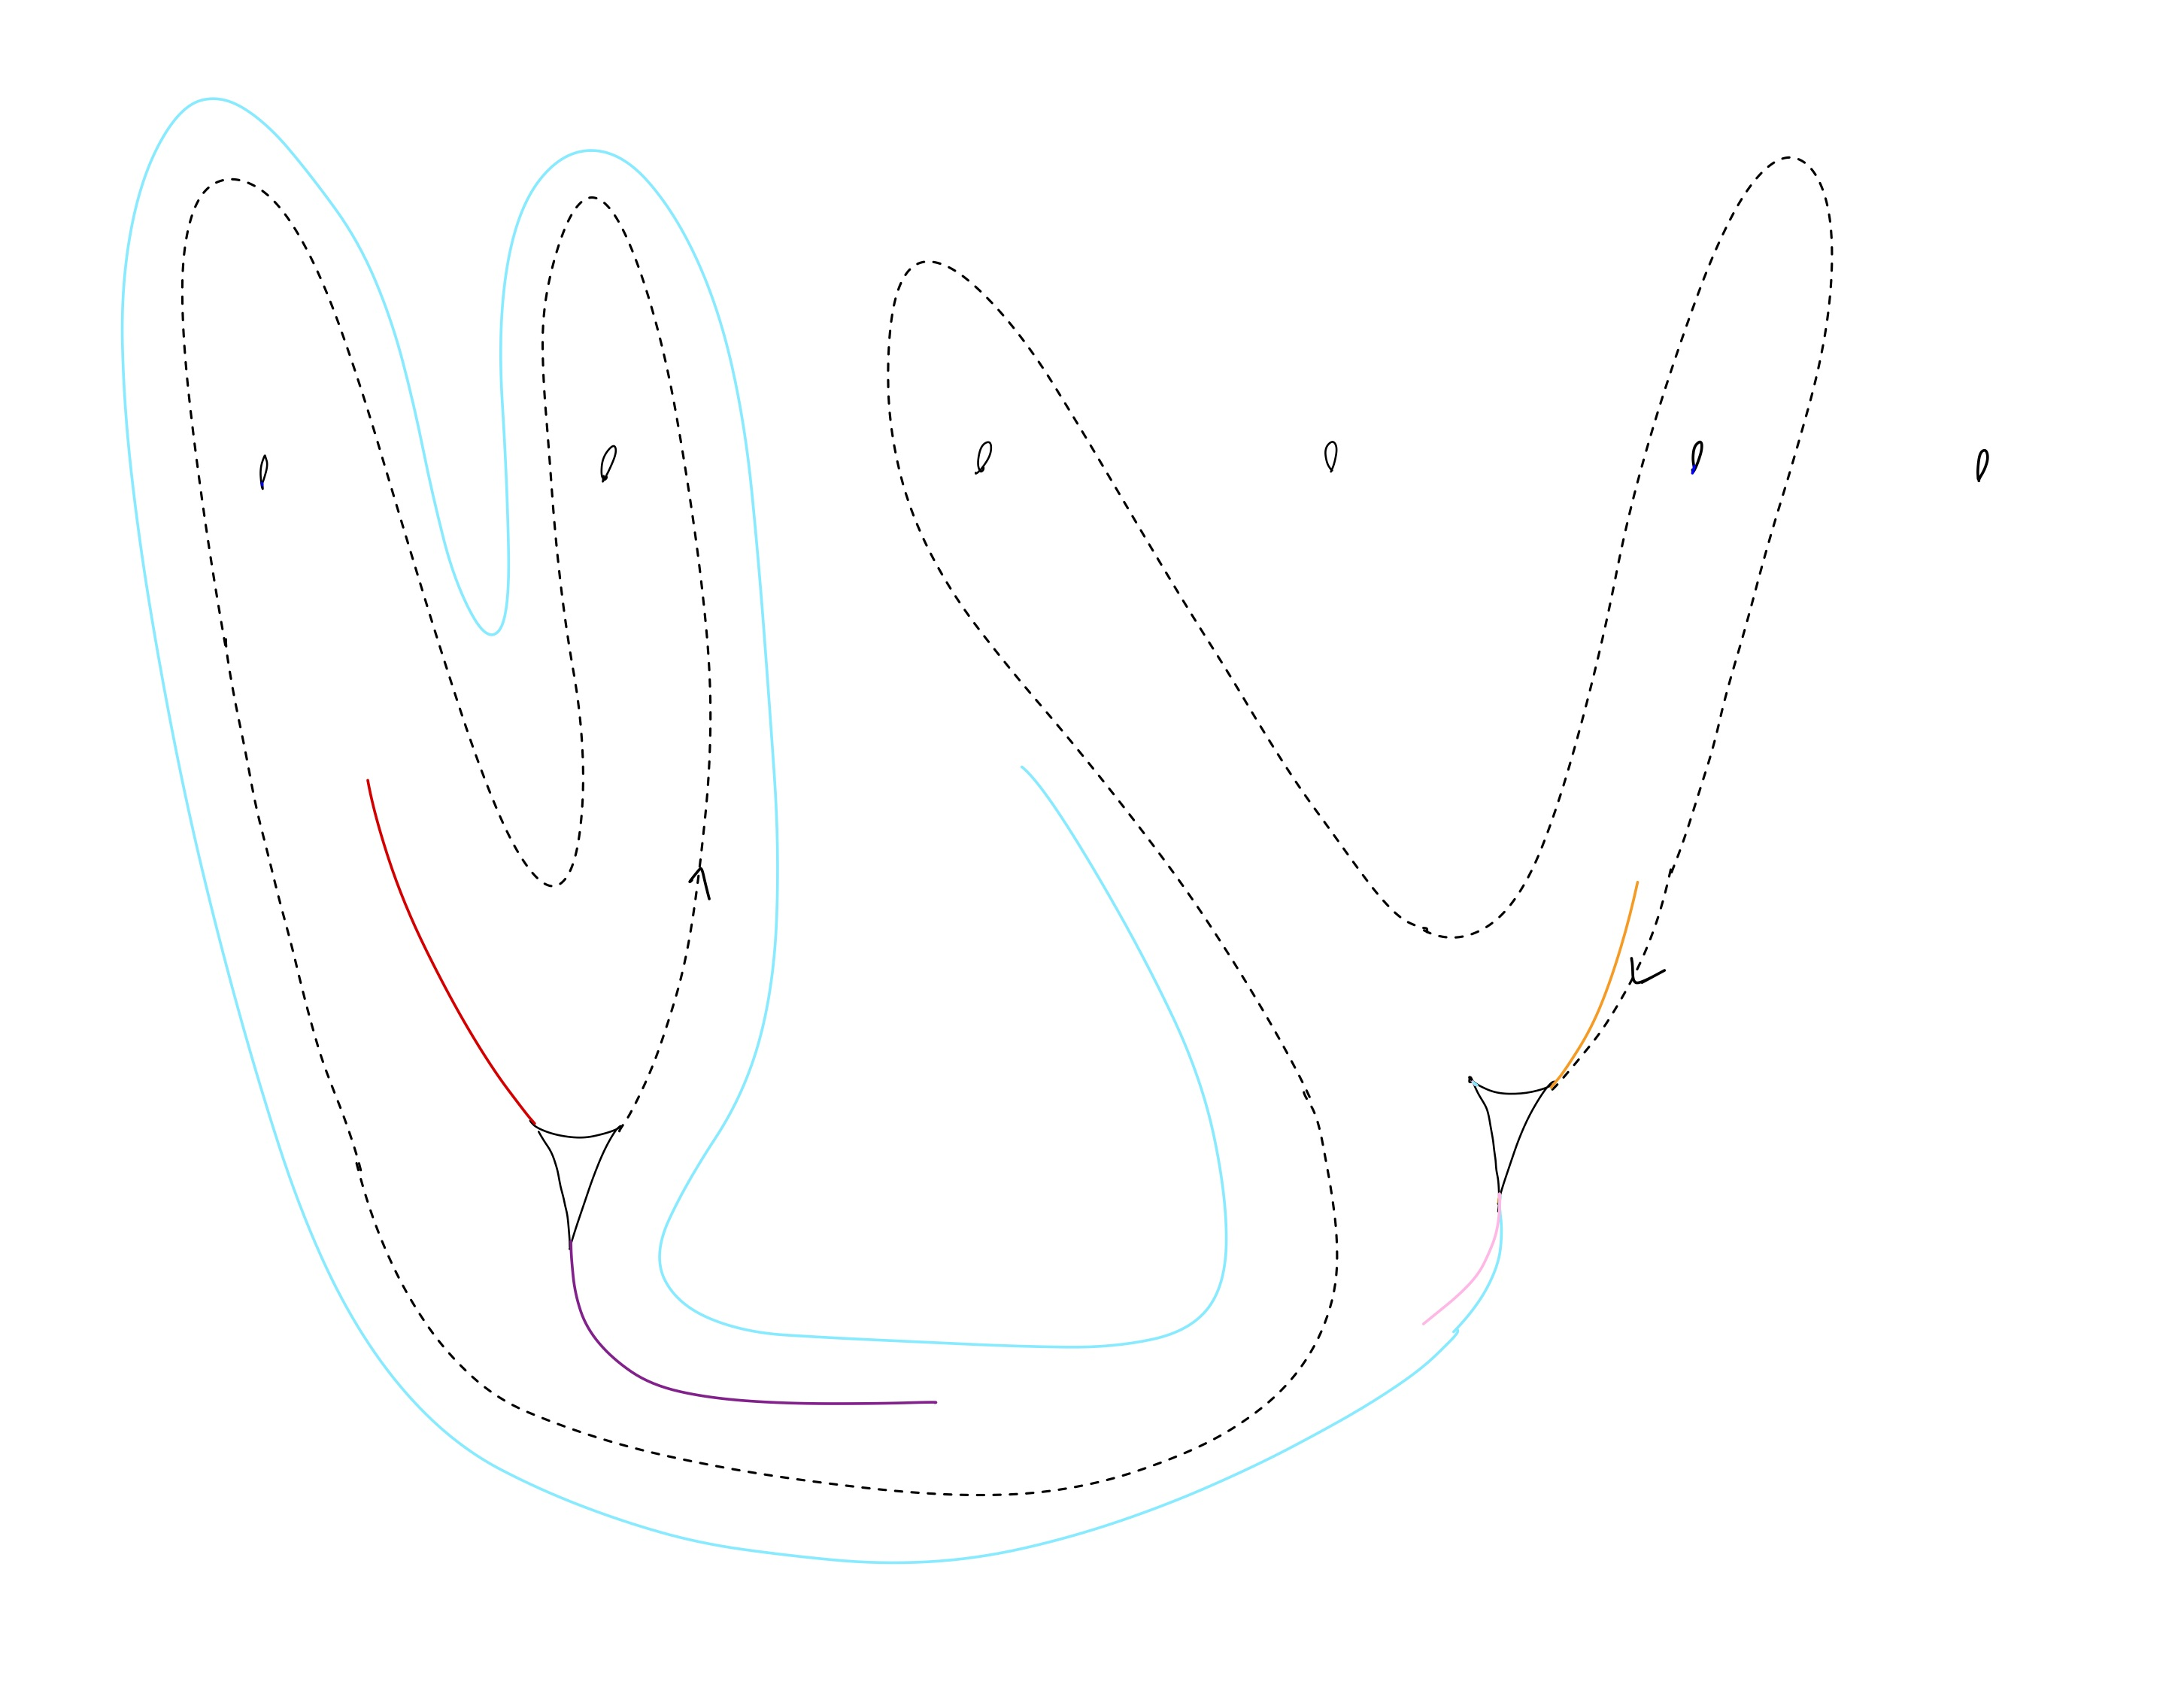
\includegraphics[width=\linewidth]{figures_case_analysis/track17_case_analysis/Blet-2.jpg}
    \caption{Blet2}
    \label{fig:Blet2}
\end{figure}

\begin{figure}[ht]
    \centering
    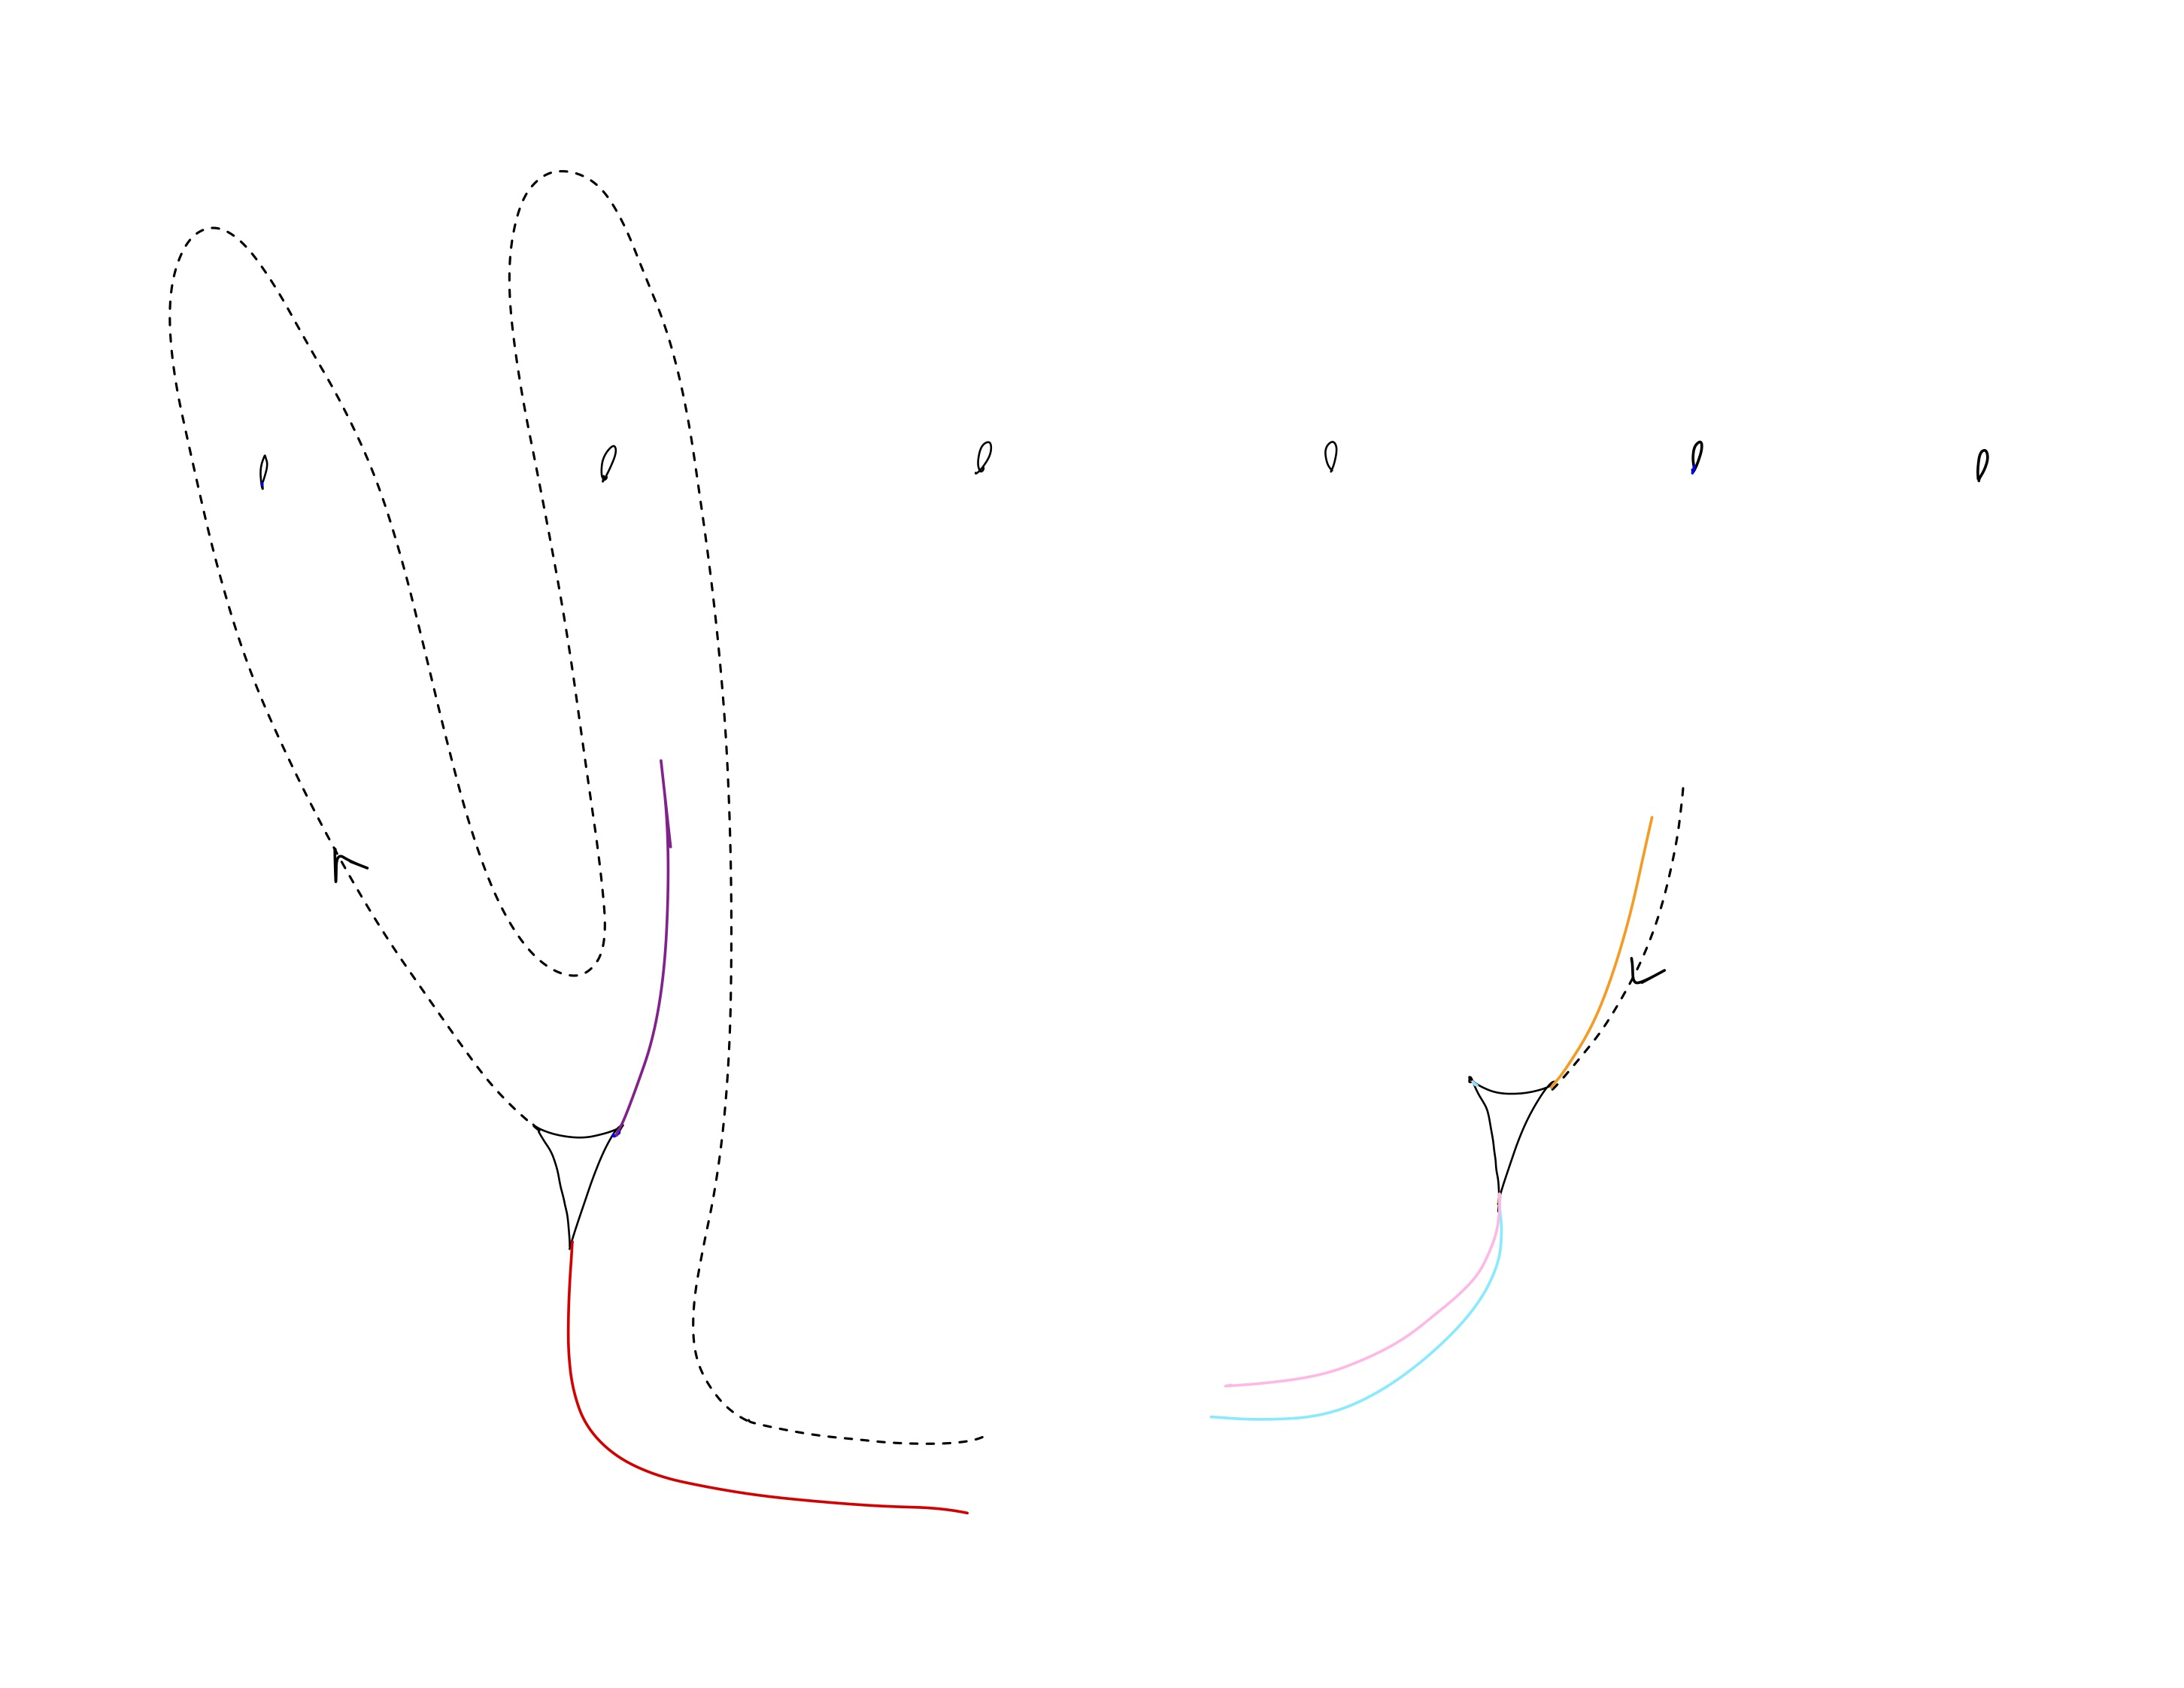
\includegraphics[width=\linewidth]{figures_case_analysis/track17_case_analysis/HLE.jpg}
    \caption{HLE1}
    \label{fig:HLE1}
\end{figure}

\begin{figure}[ht]
    \centering
    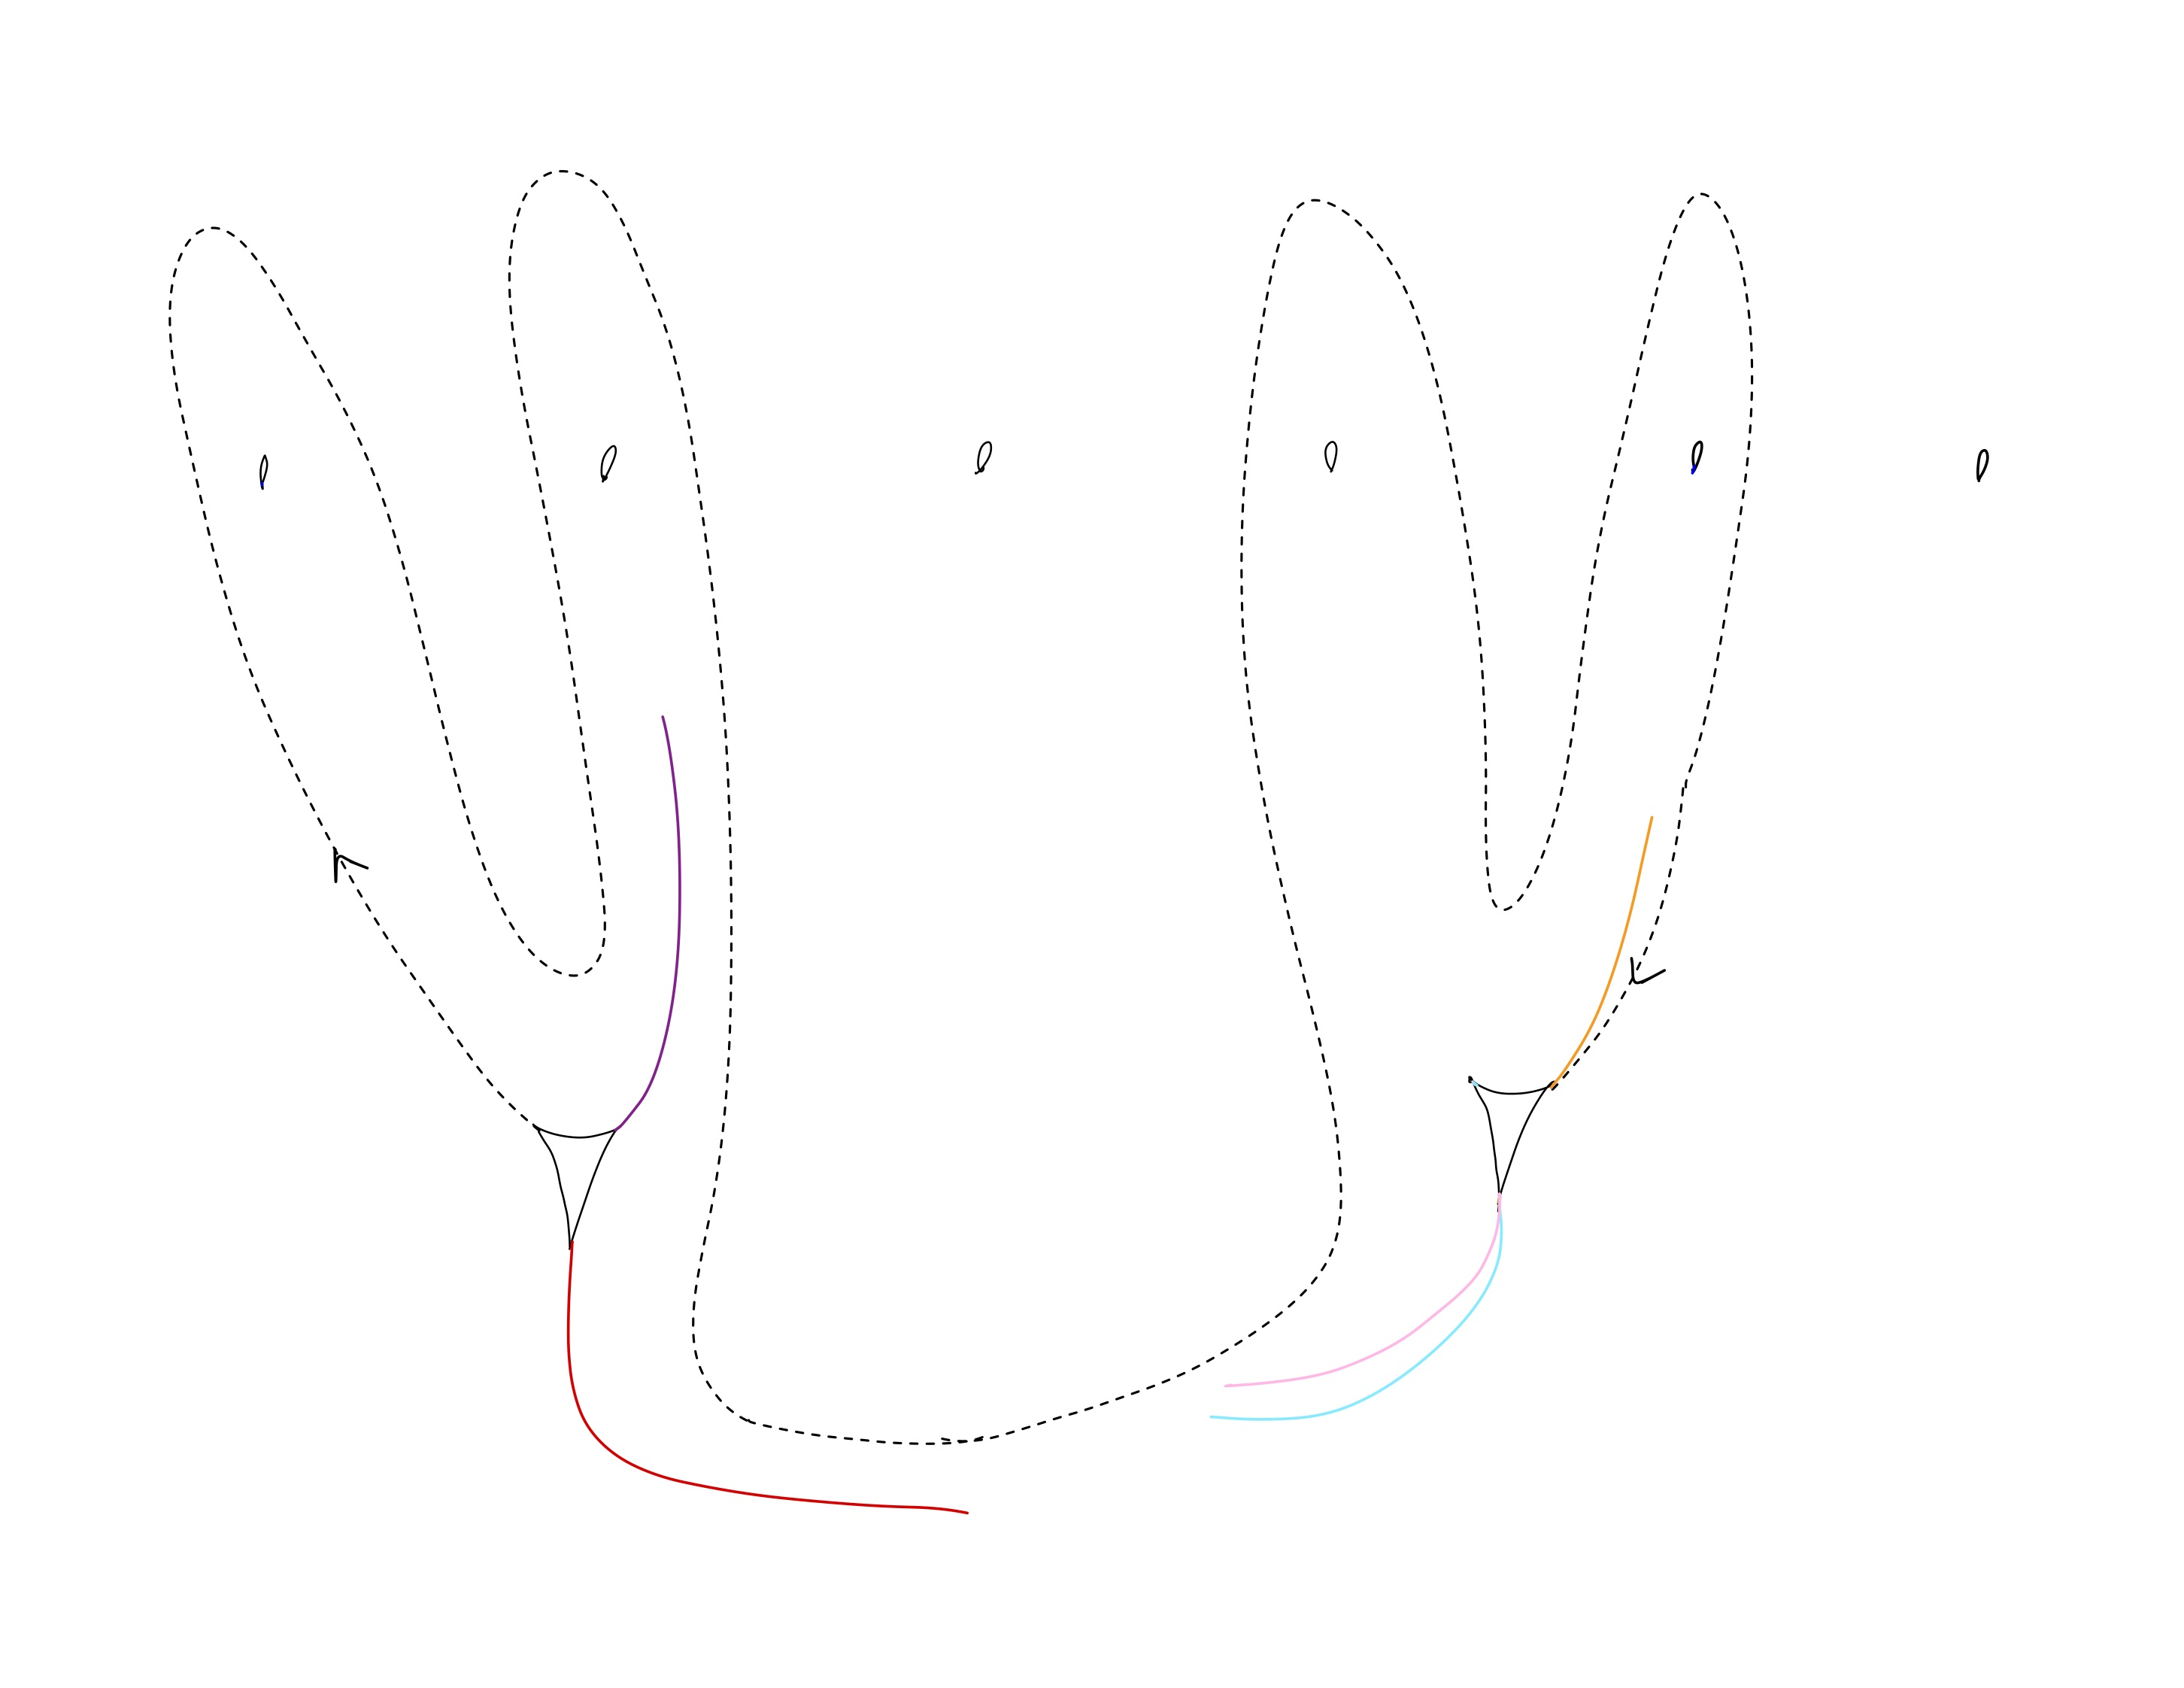
\includegraphics[width=\linewidth]{figures_case_analysis/track17_case_analysis/Dree-1.jpg}
    \caption{Dree1}
    \label{fig:Dree1}
\end{figure}

\begin{figure}[ht]
    \centering
    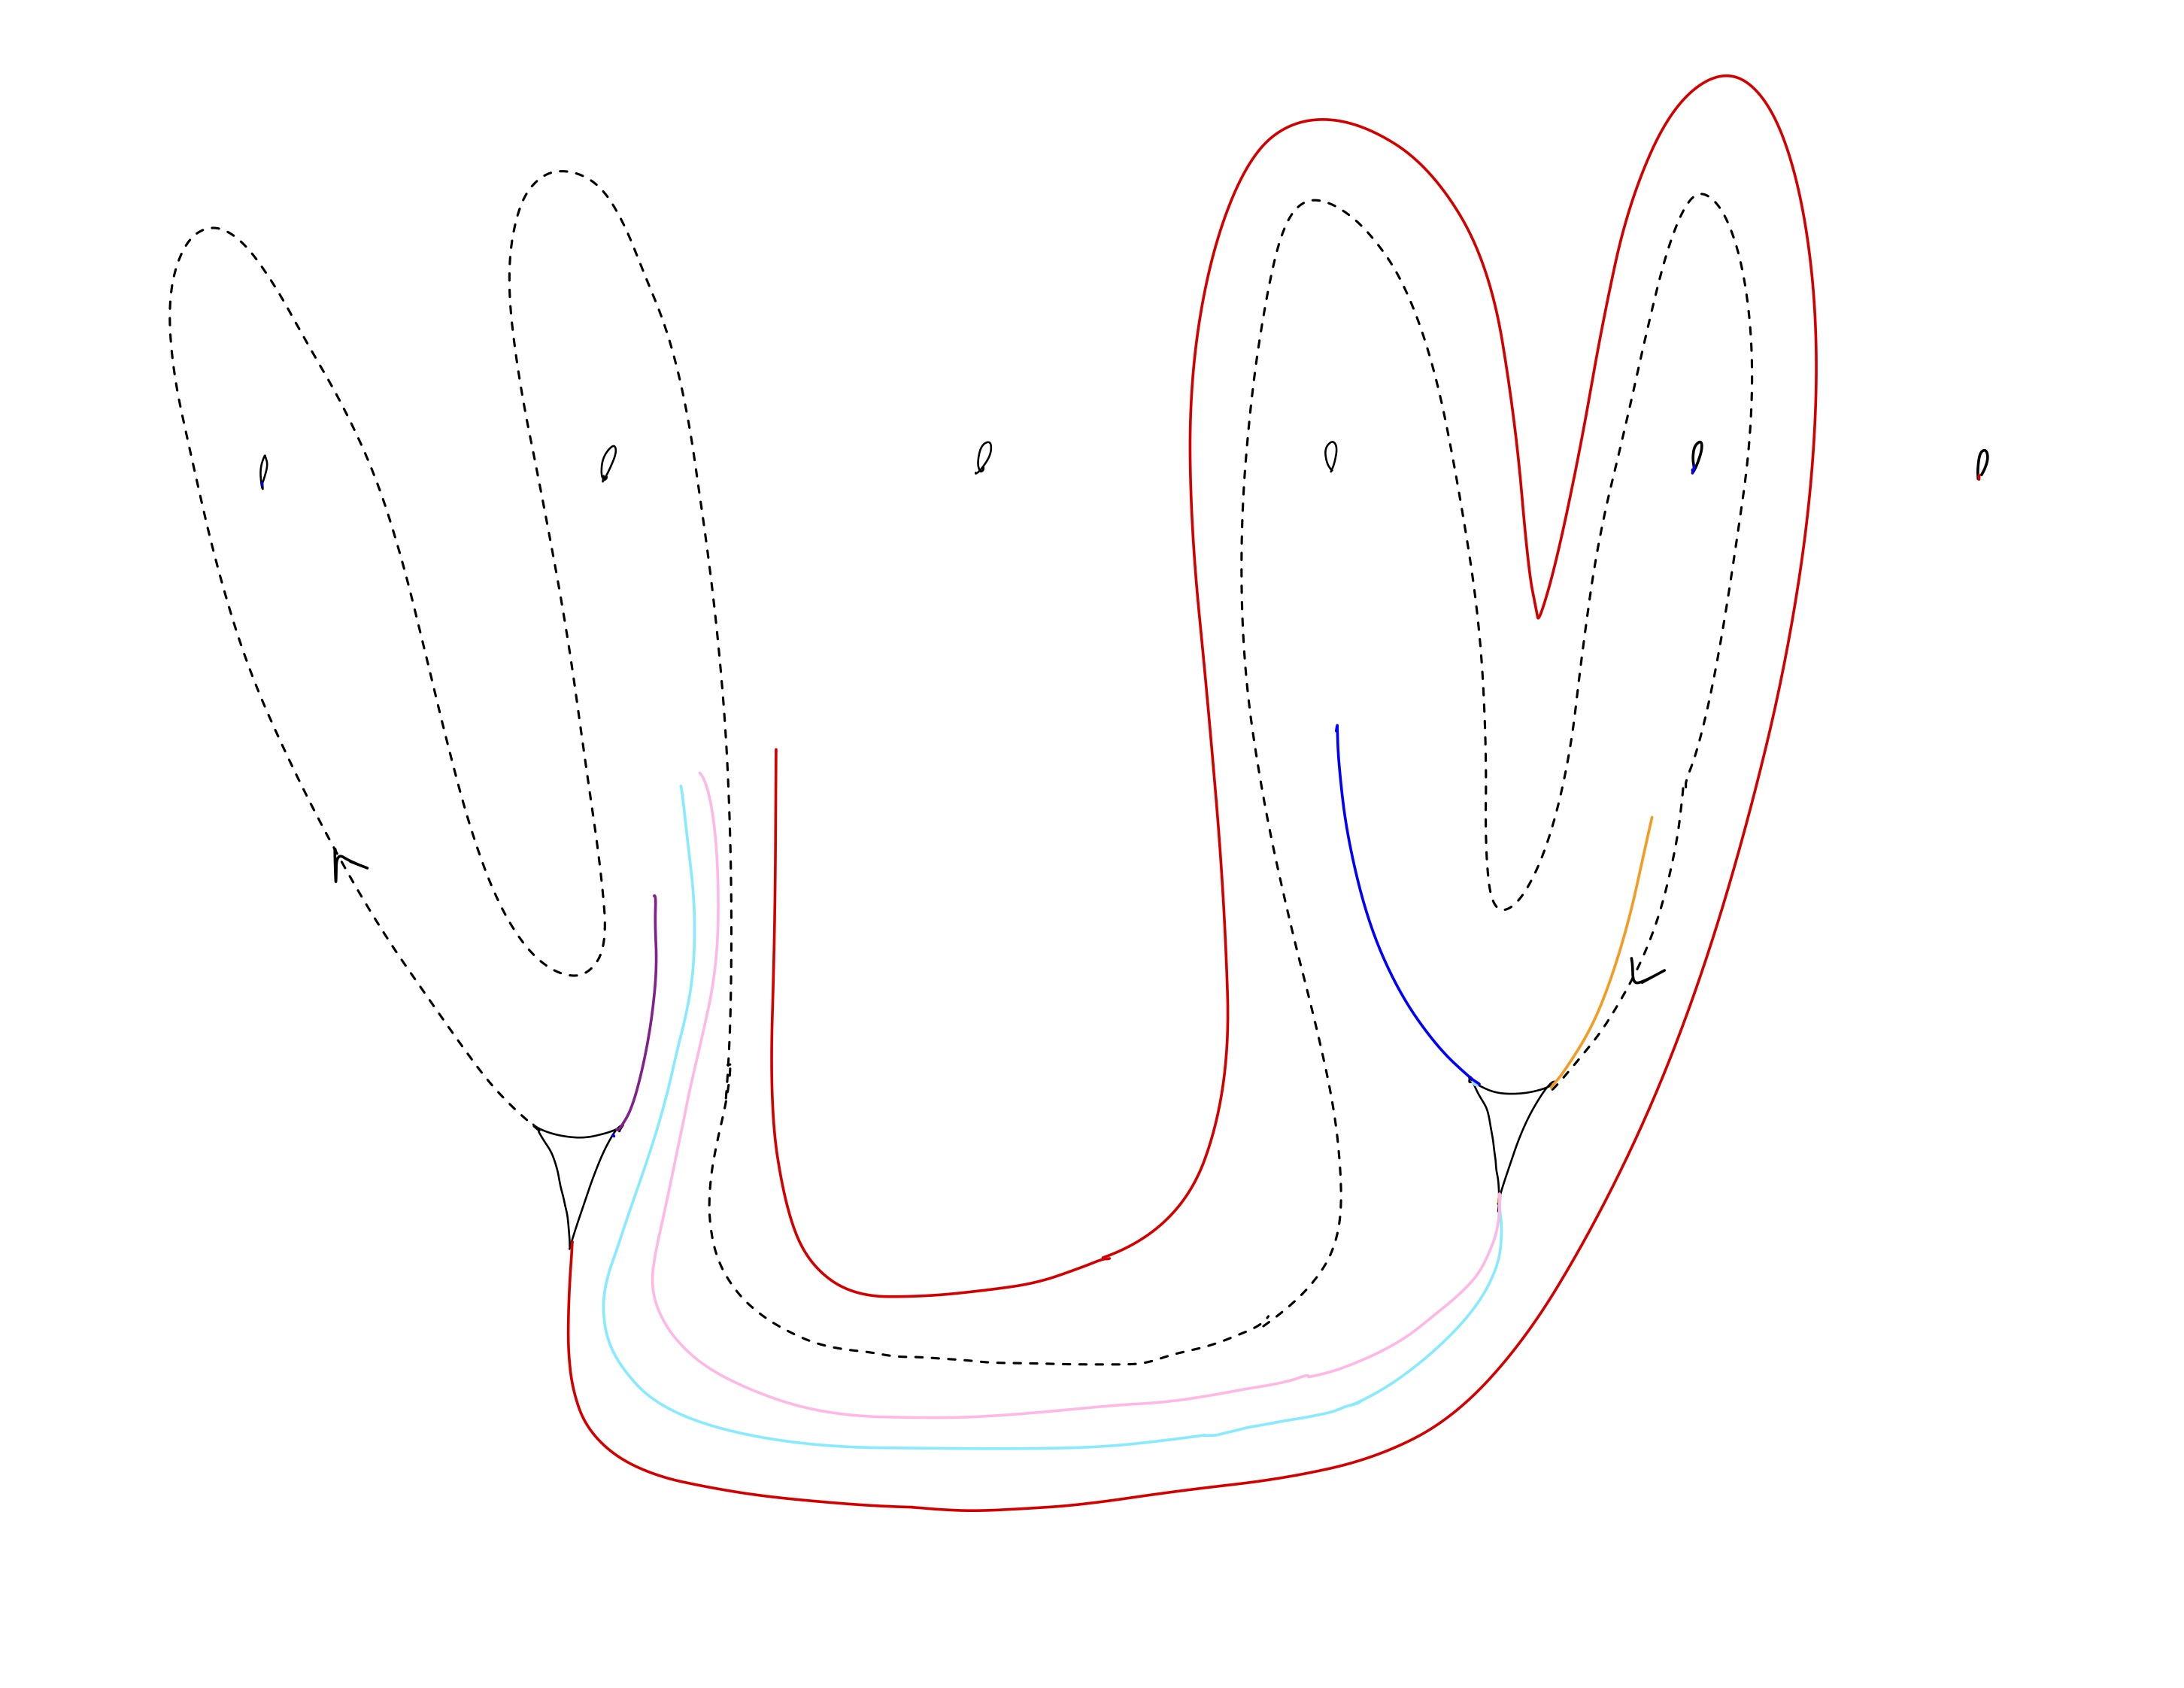
\includegraphics[width=\linewidth]{figures_case_analysis/track17_case_analysis/Dree-2.jpg}
    \caption{Dree2}
    \label{fig:Dree2}
\end{figure}
\clearpage

\begin{figure}[ht]
    \centering
    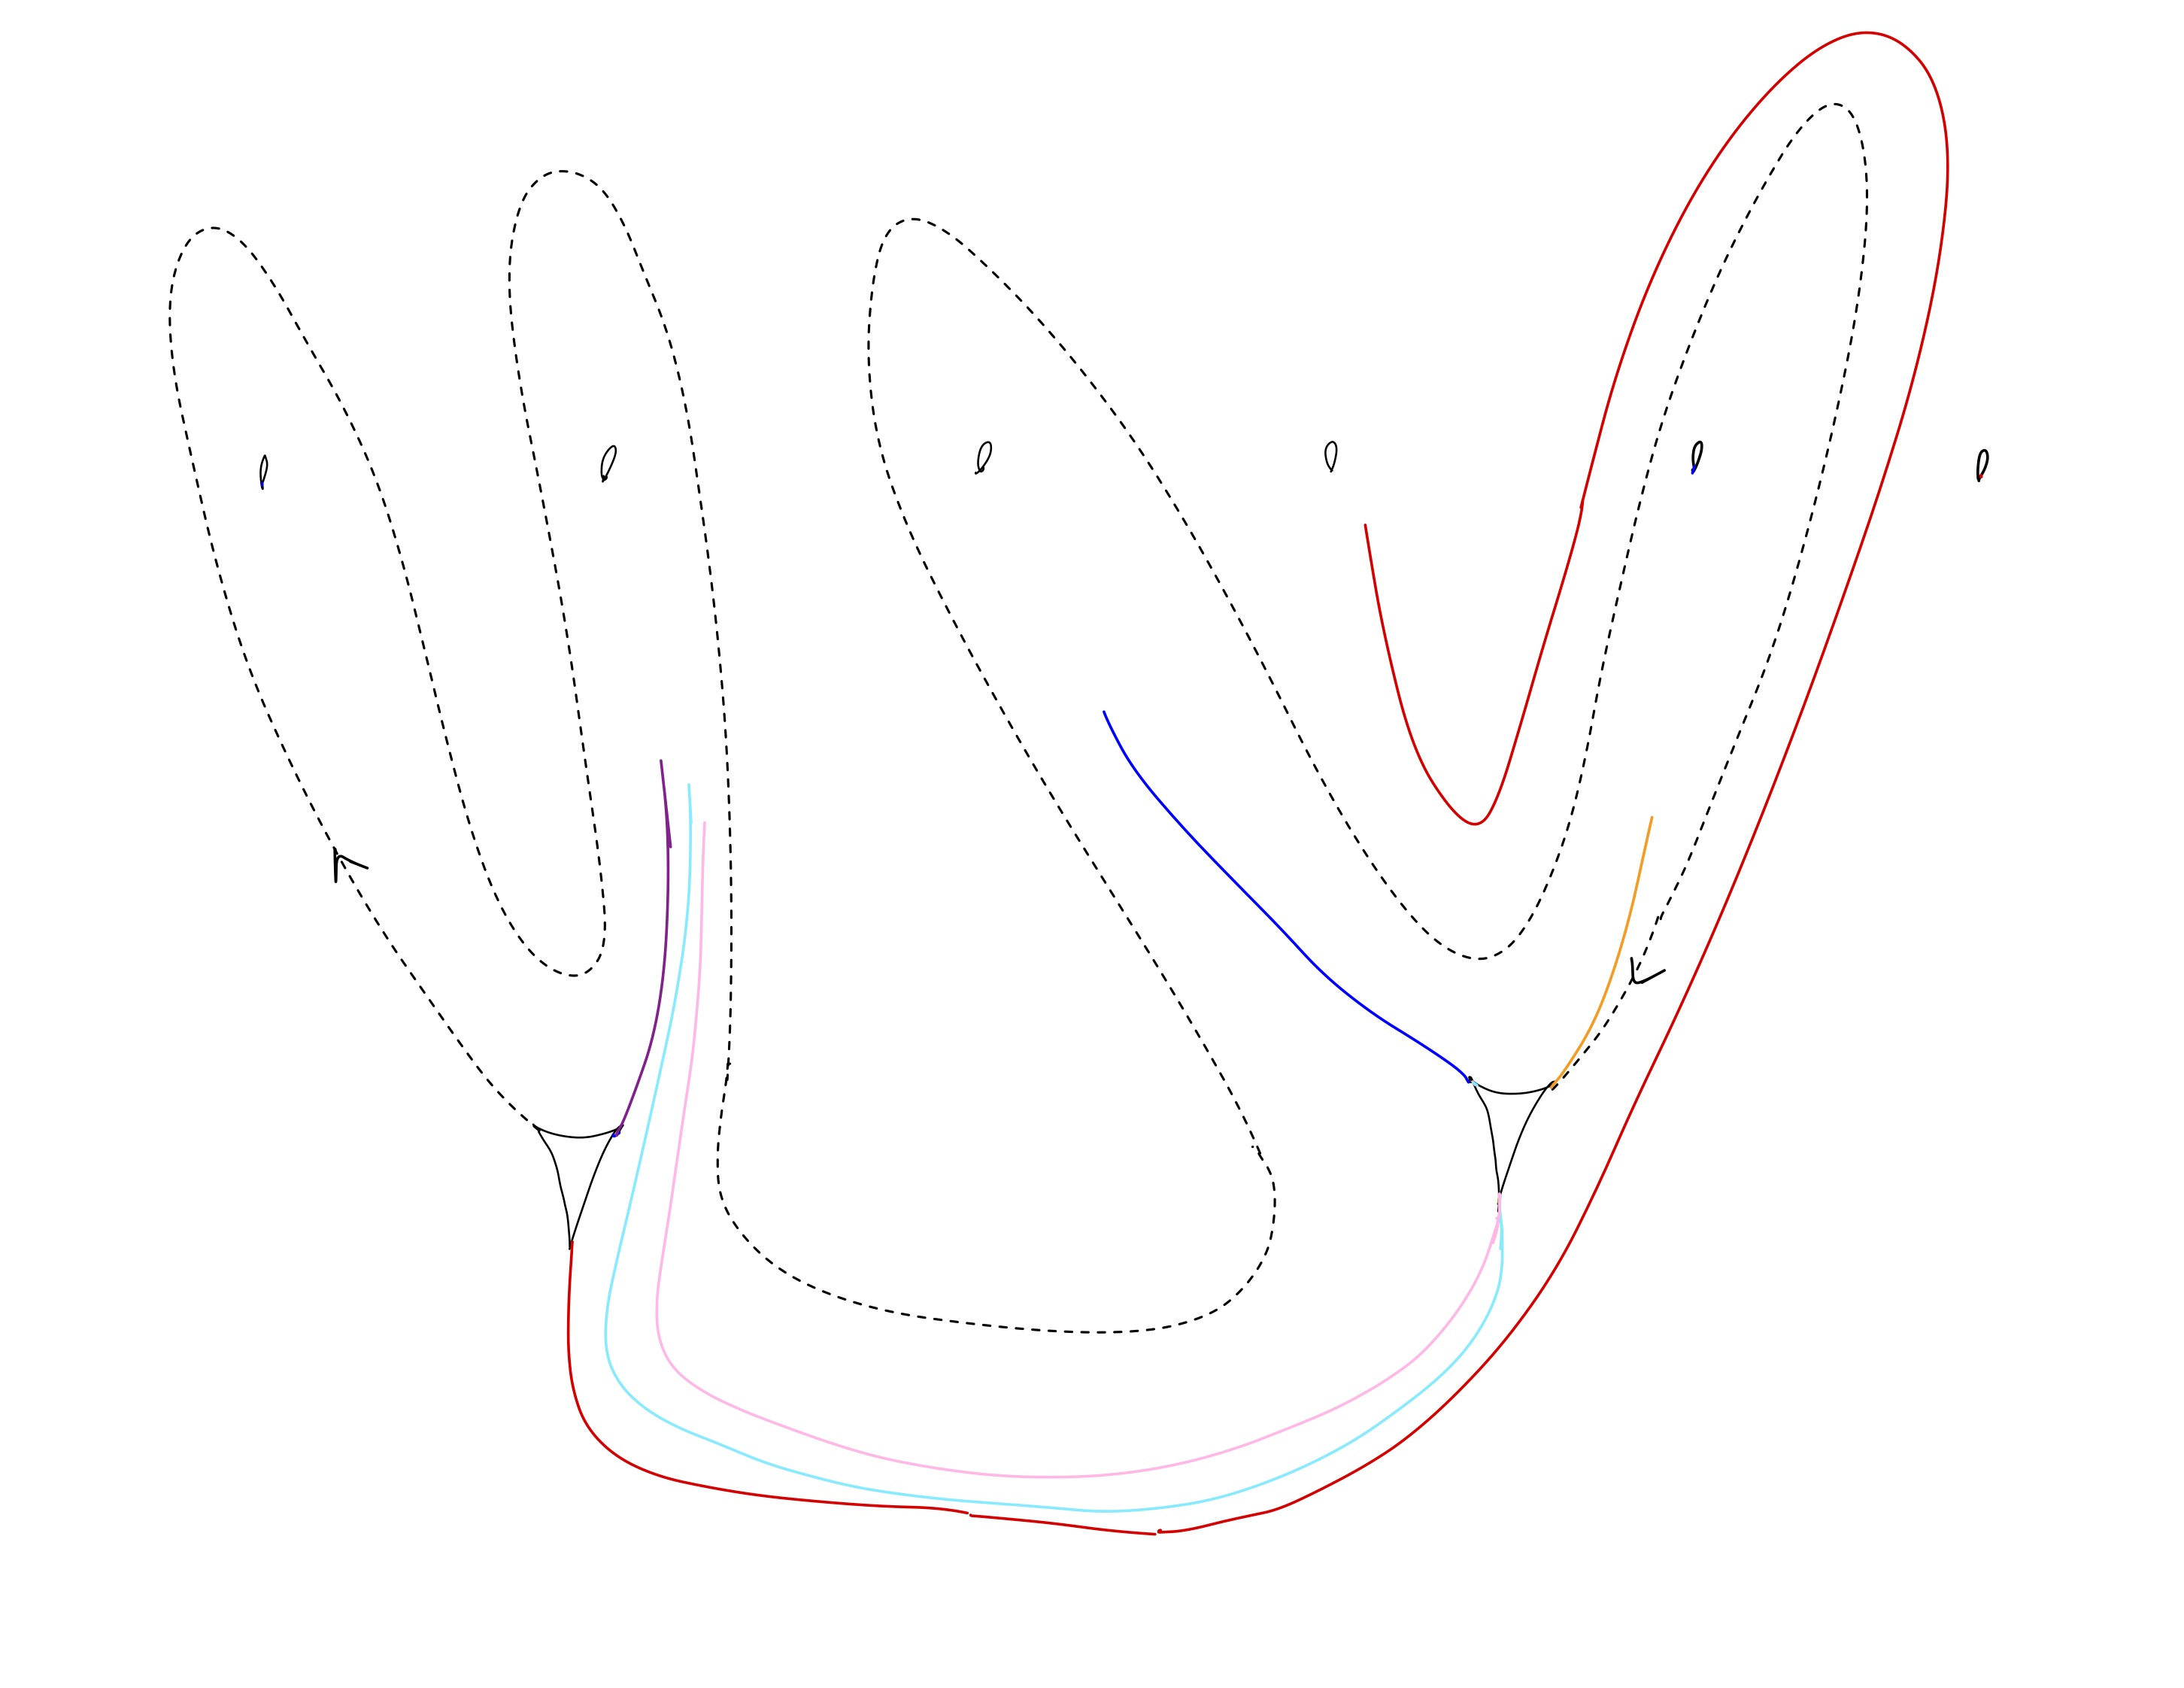
\includegraphics[width=\linewidth]{figures_case_analysis/track17_case_analysis/Moke-1.jpg}
    \caption{Moke1}
    \label{fig:Moke1}
\end{figure}

\begin{figure}[ht]
    \centering
    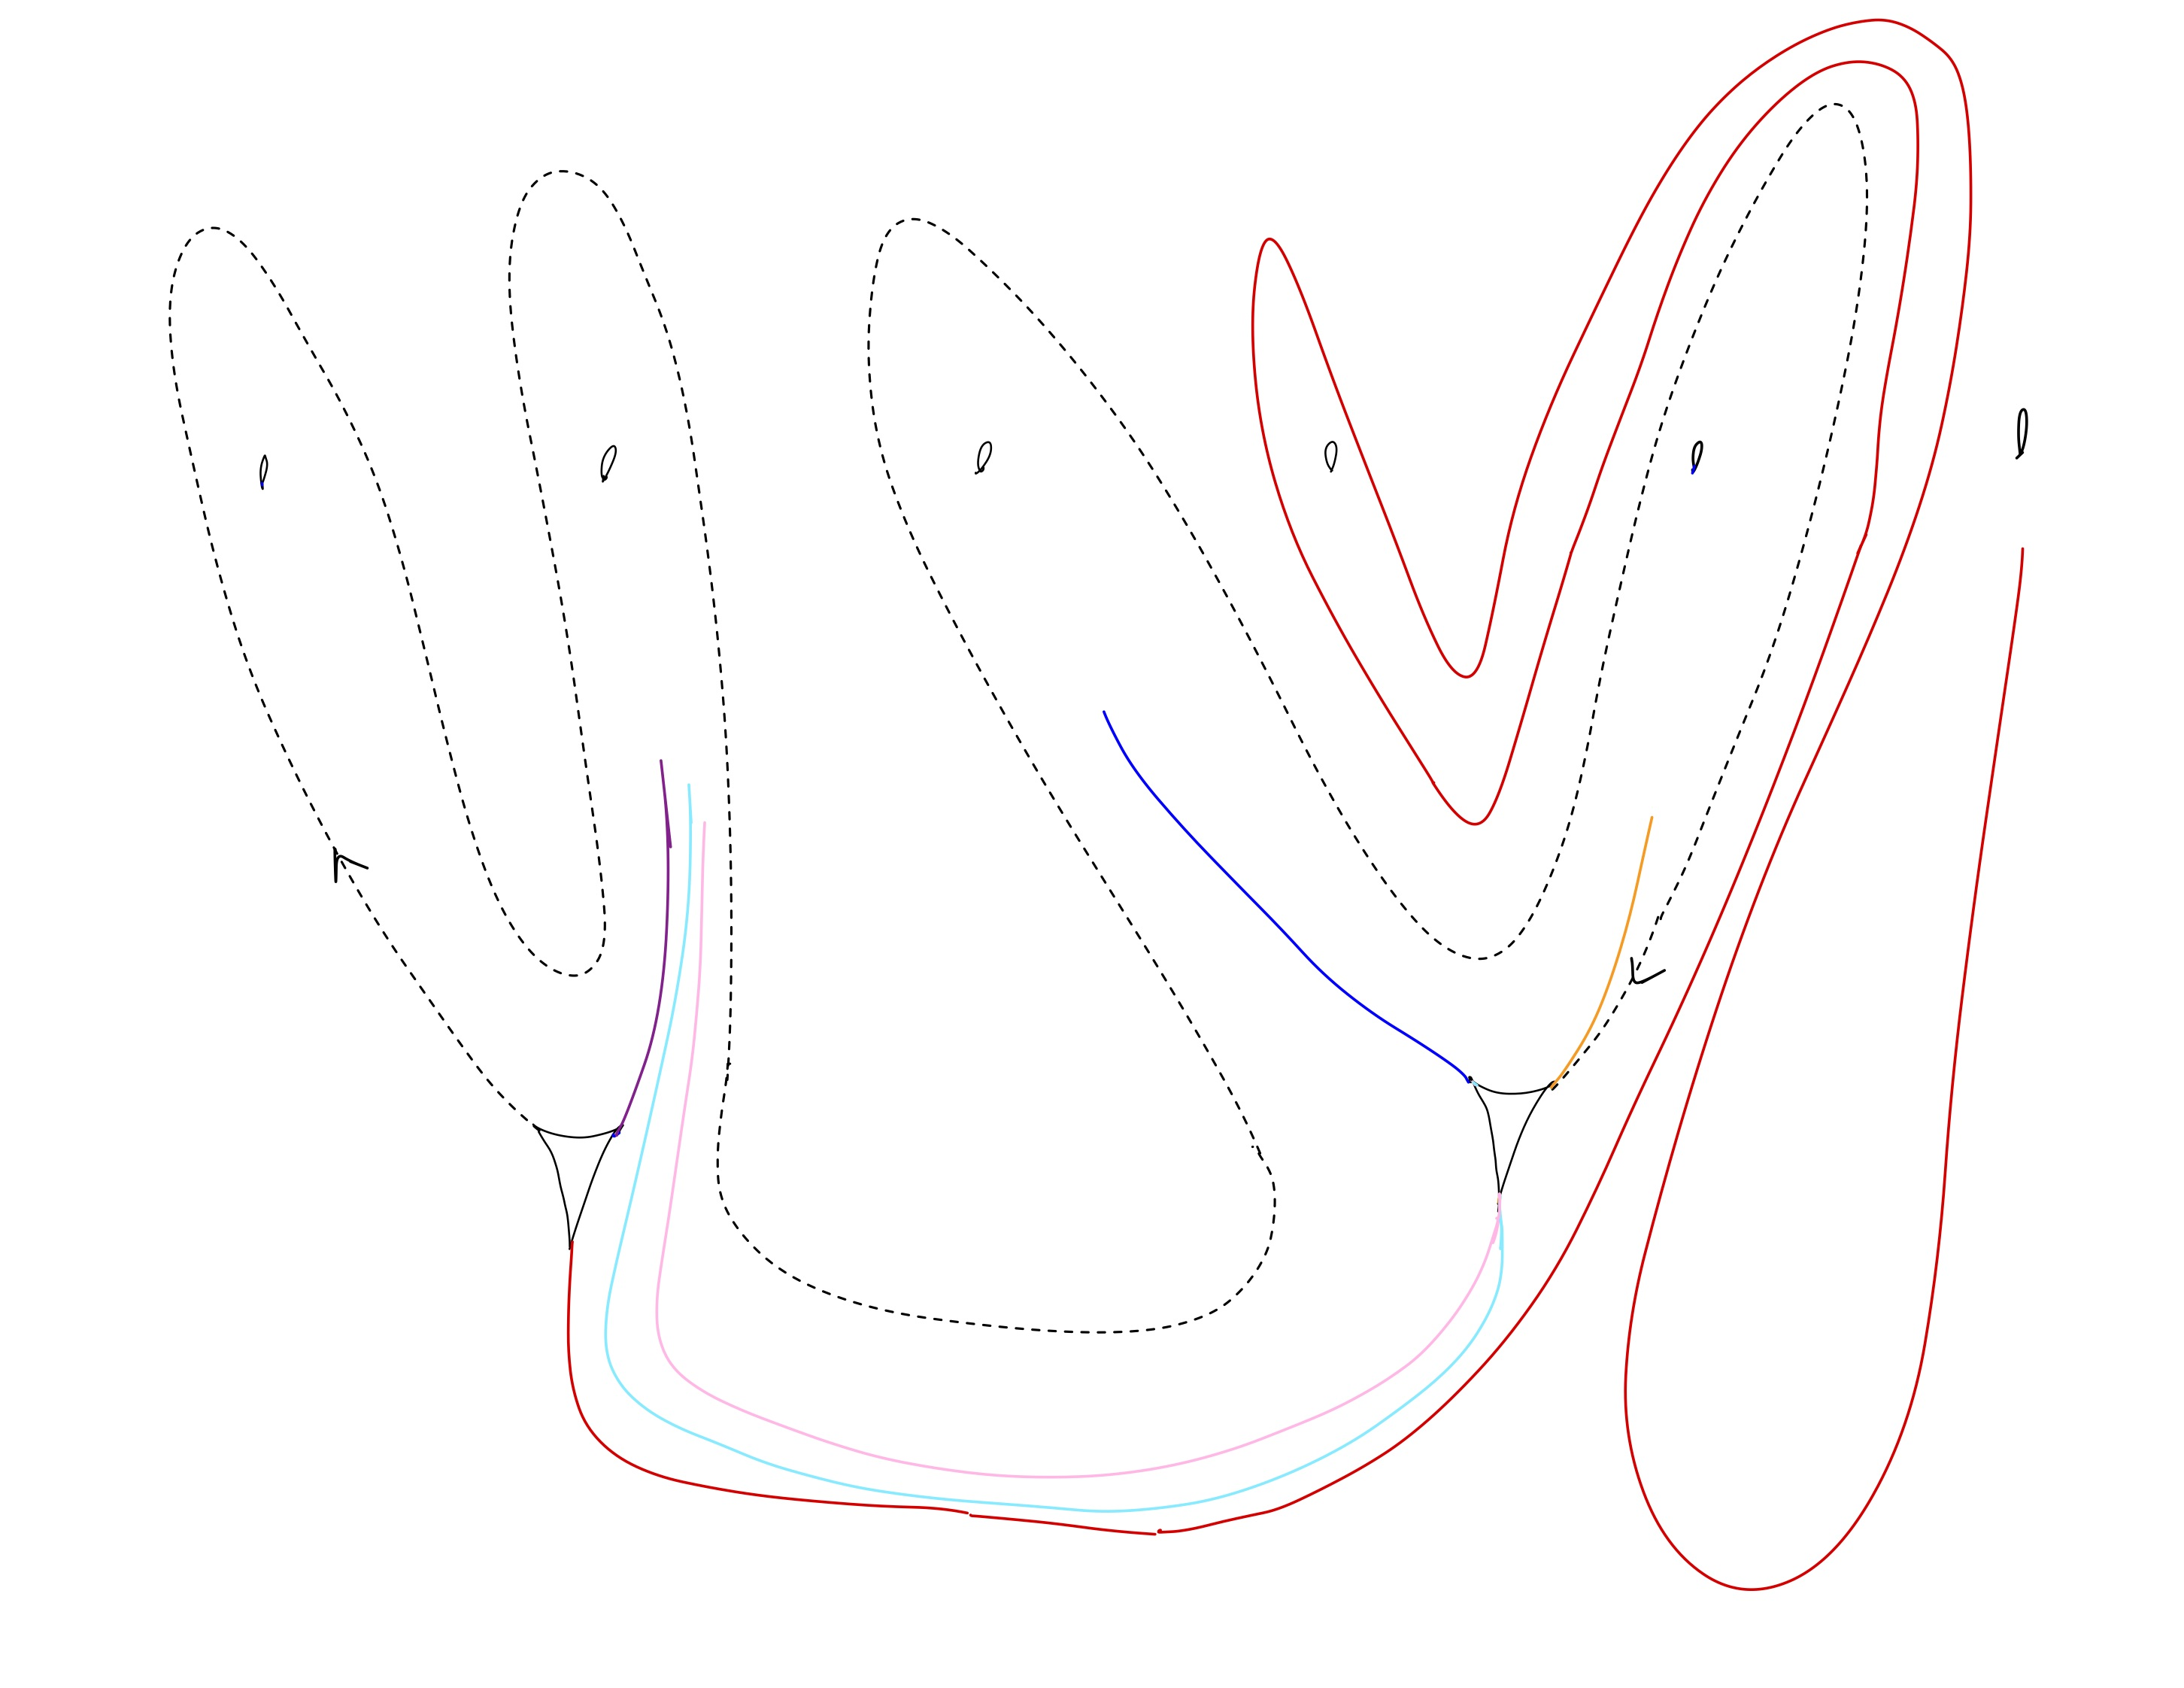
\includegraphics[width=\linewidth]{figures_case_analysis/track17_case_analysis/Moke-2.jpg}
    \caption{Moke2}
    \label{fig:Moke2}
\end{figure}

\begin{figure}[ht]
    \centering
    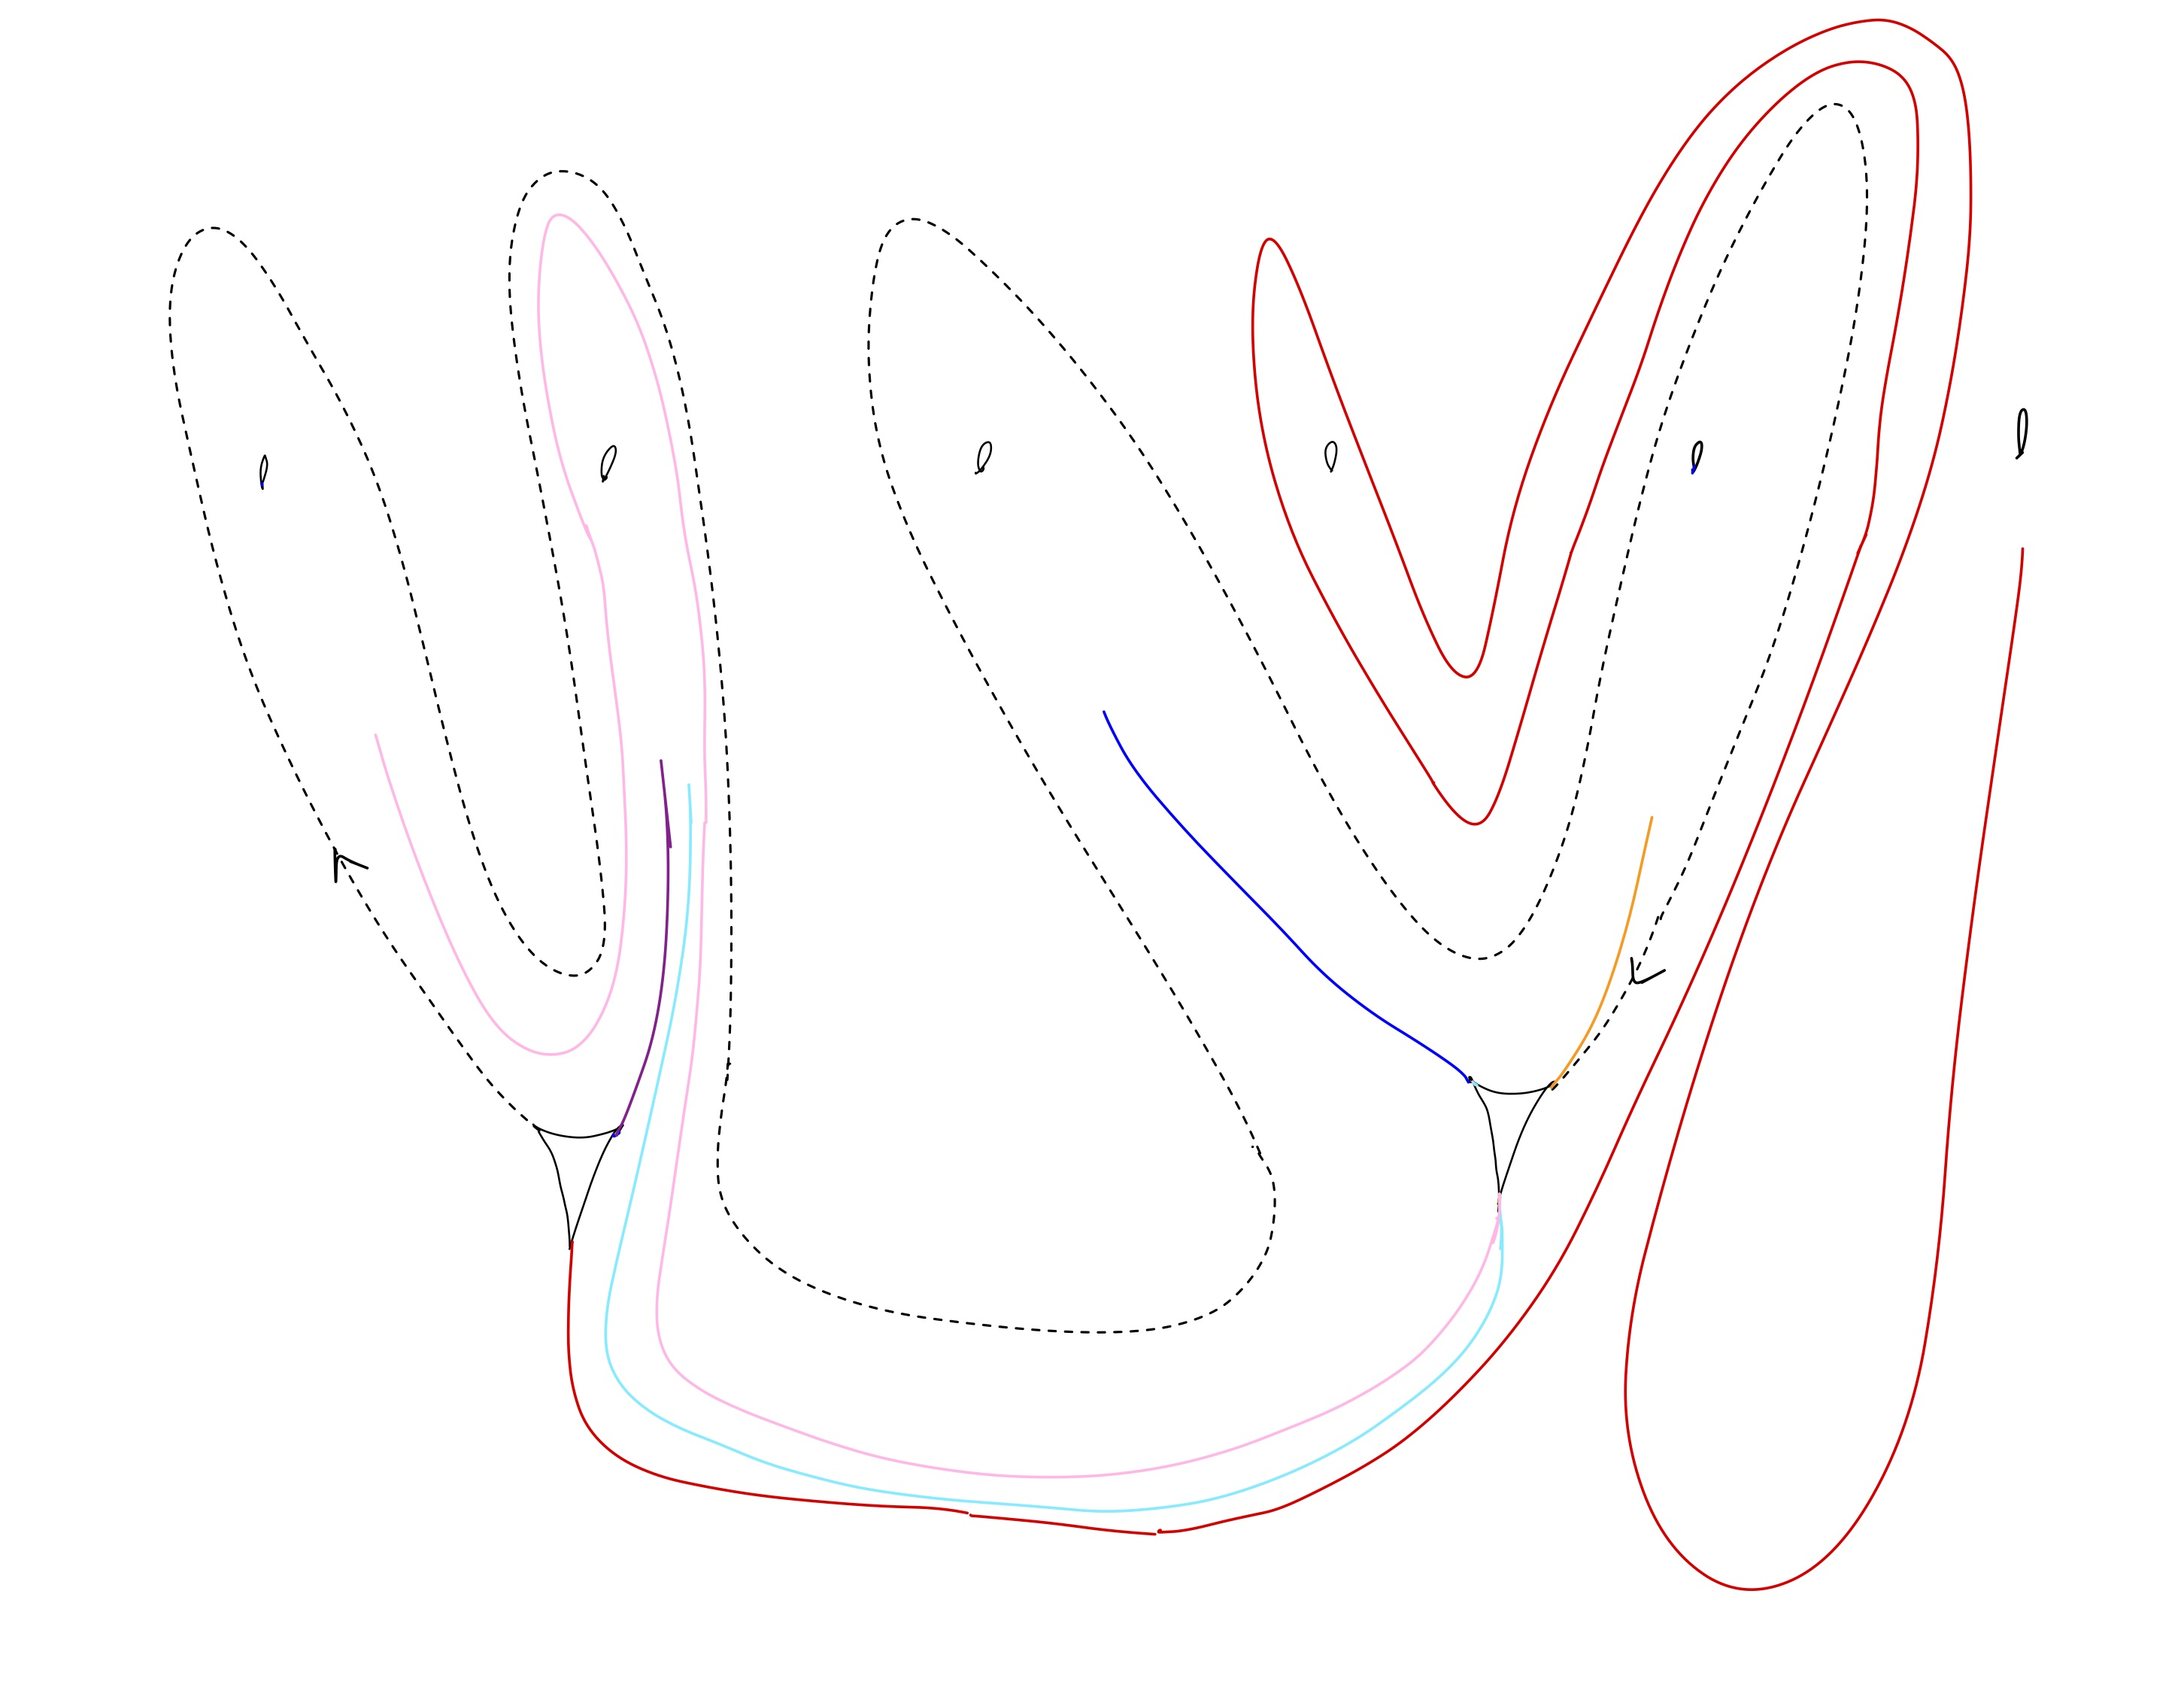
\includegraphics[width=\linewidth]{figures_case_analysis/track17_case_analysis/Moke-3.jpg}
    \caption{Moke3}
    \label{fig:Moke3}
\end{figure}

\begin{figure}[ht]
    \centering
    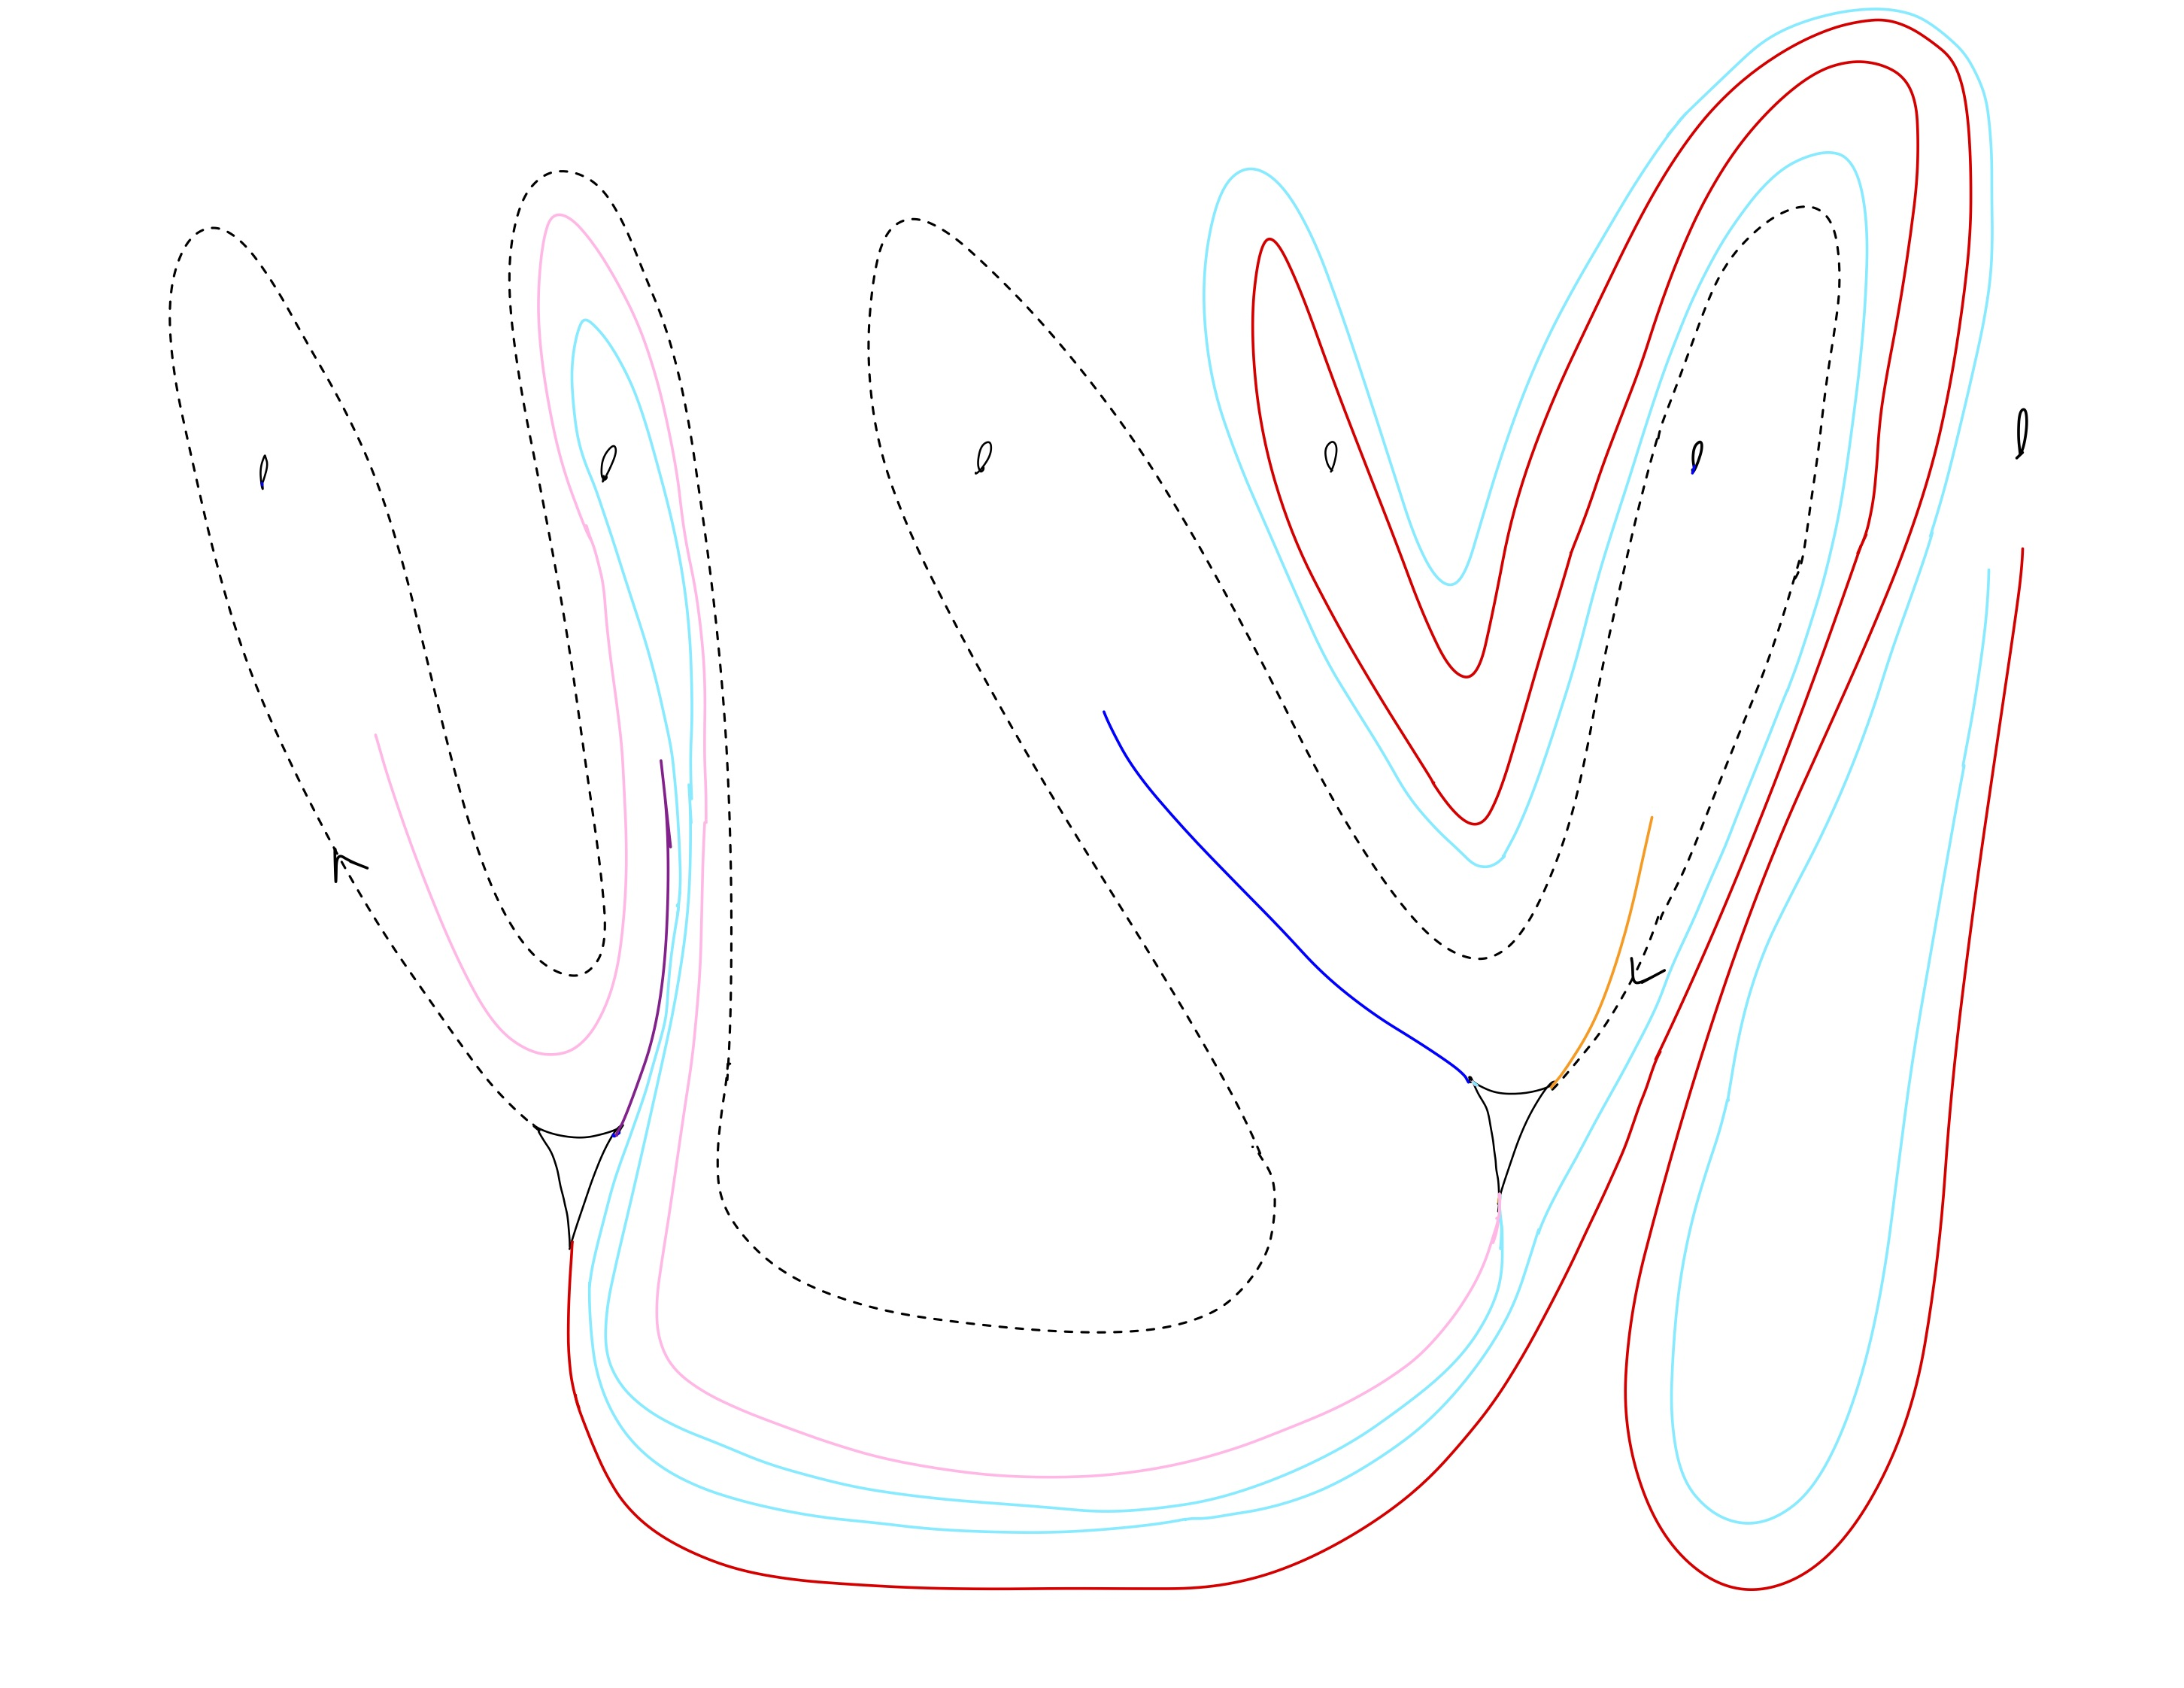
\includegraphics[width=\linewidth]{figures_case_analysis/track17_case_analysis/Moke-4.jpg}
    \caption{Moke4}
    \label{fig:Moke4}
\end{figure}

\begin{figure}[ht]
    \centering
    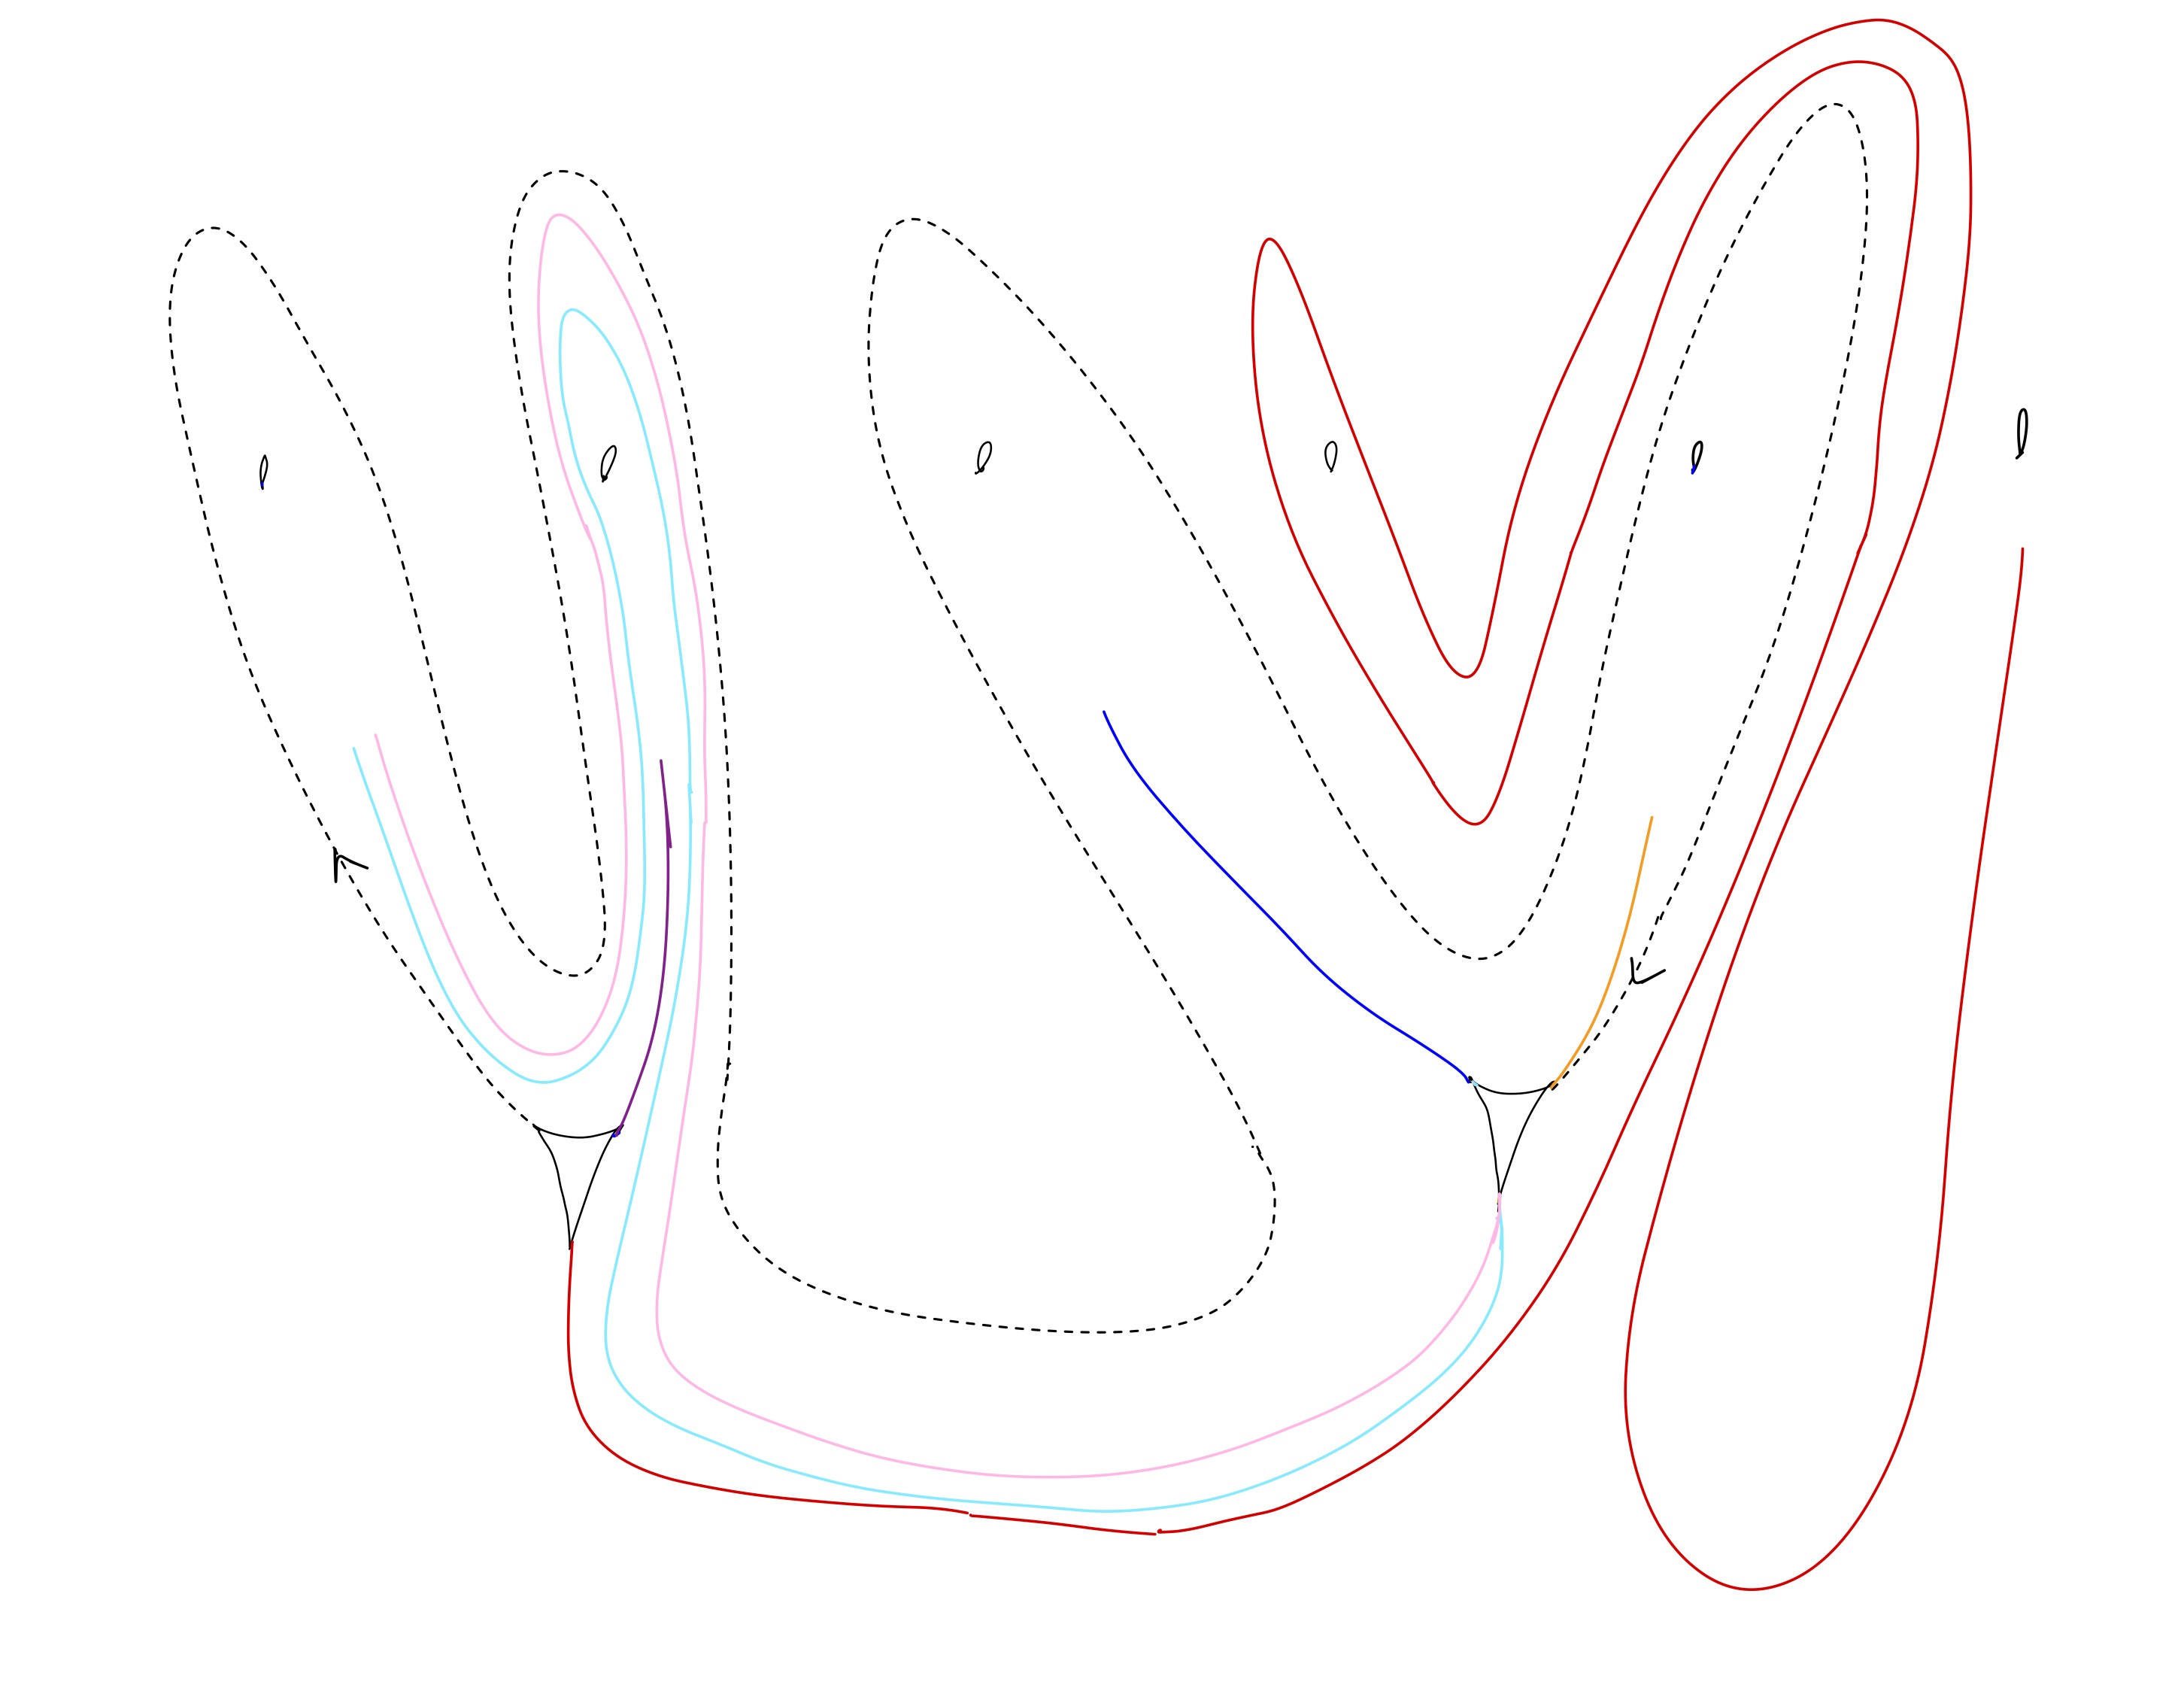
\includegraphics[width=\linewidth]{figures_case_analysis/track17_case_analysis/Moke-5.jpg}
    \caption{Moke5}
    \label{fig:Moke5}
\end{figure}

\begin{figure}[ht]
    \centering
    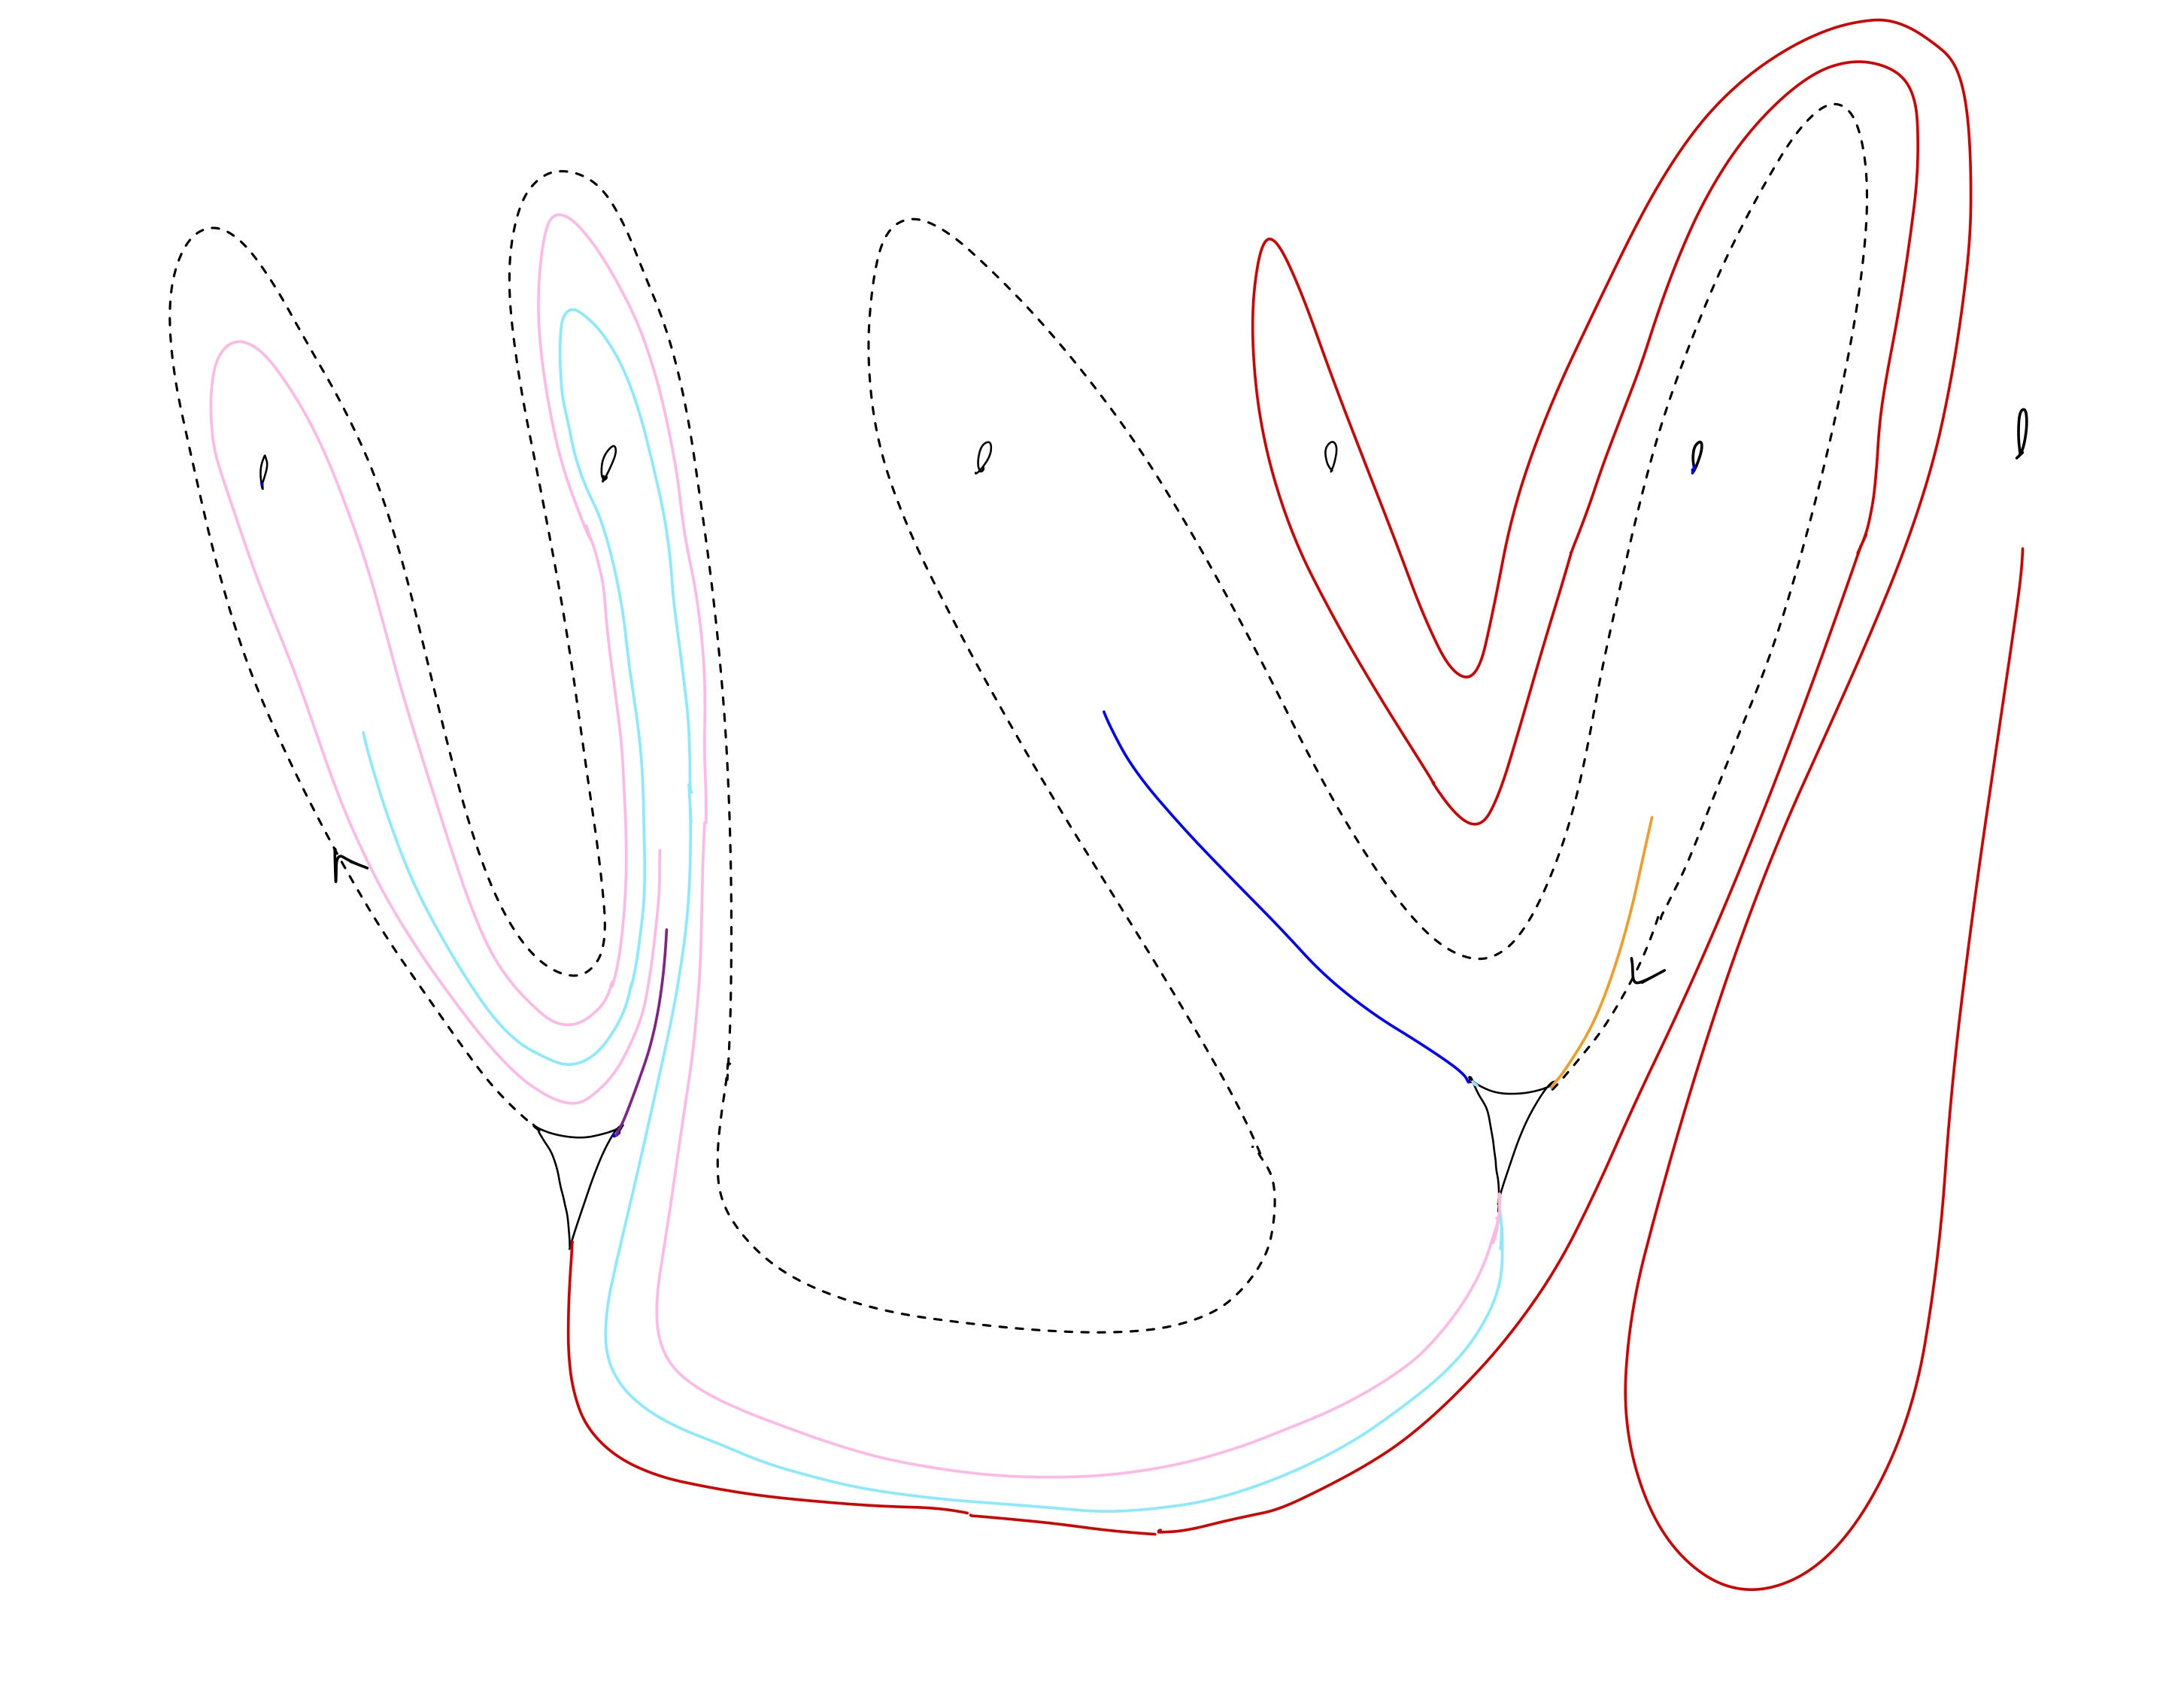
\includegraphics[width=\linewidth]{figures_case_analysis/track17_case_analysis/Moke-6.jpg}
    \caption{Moke6}
    \label{fig:Moke6}
\end{figure}

\begin{figure}[ht]
    \centering
    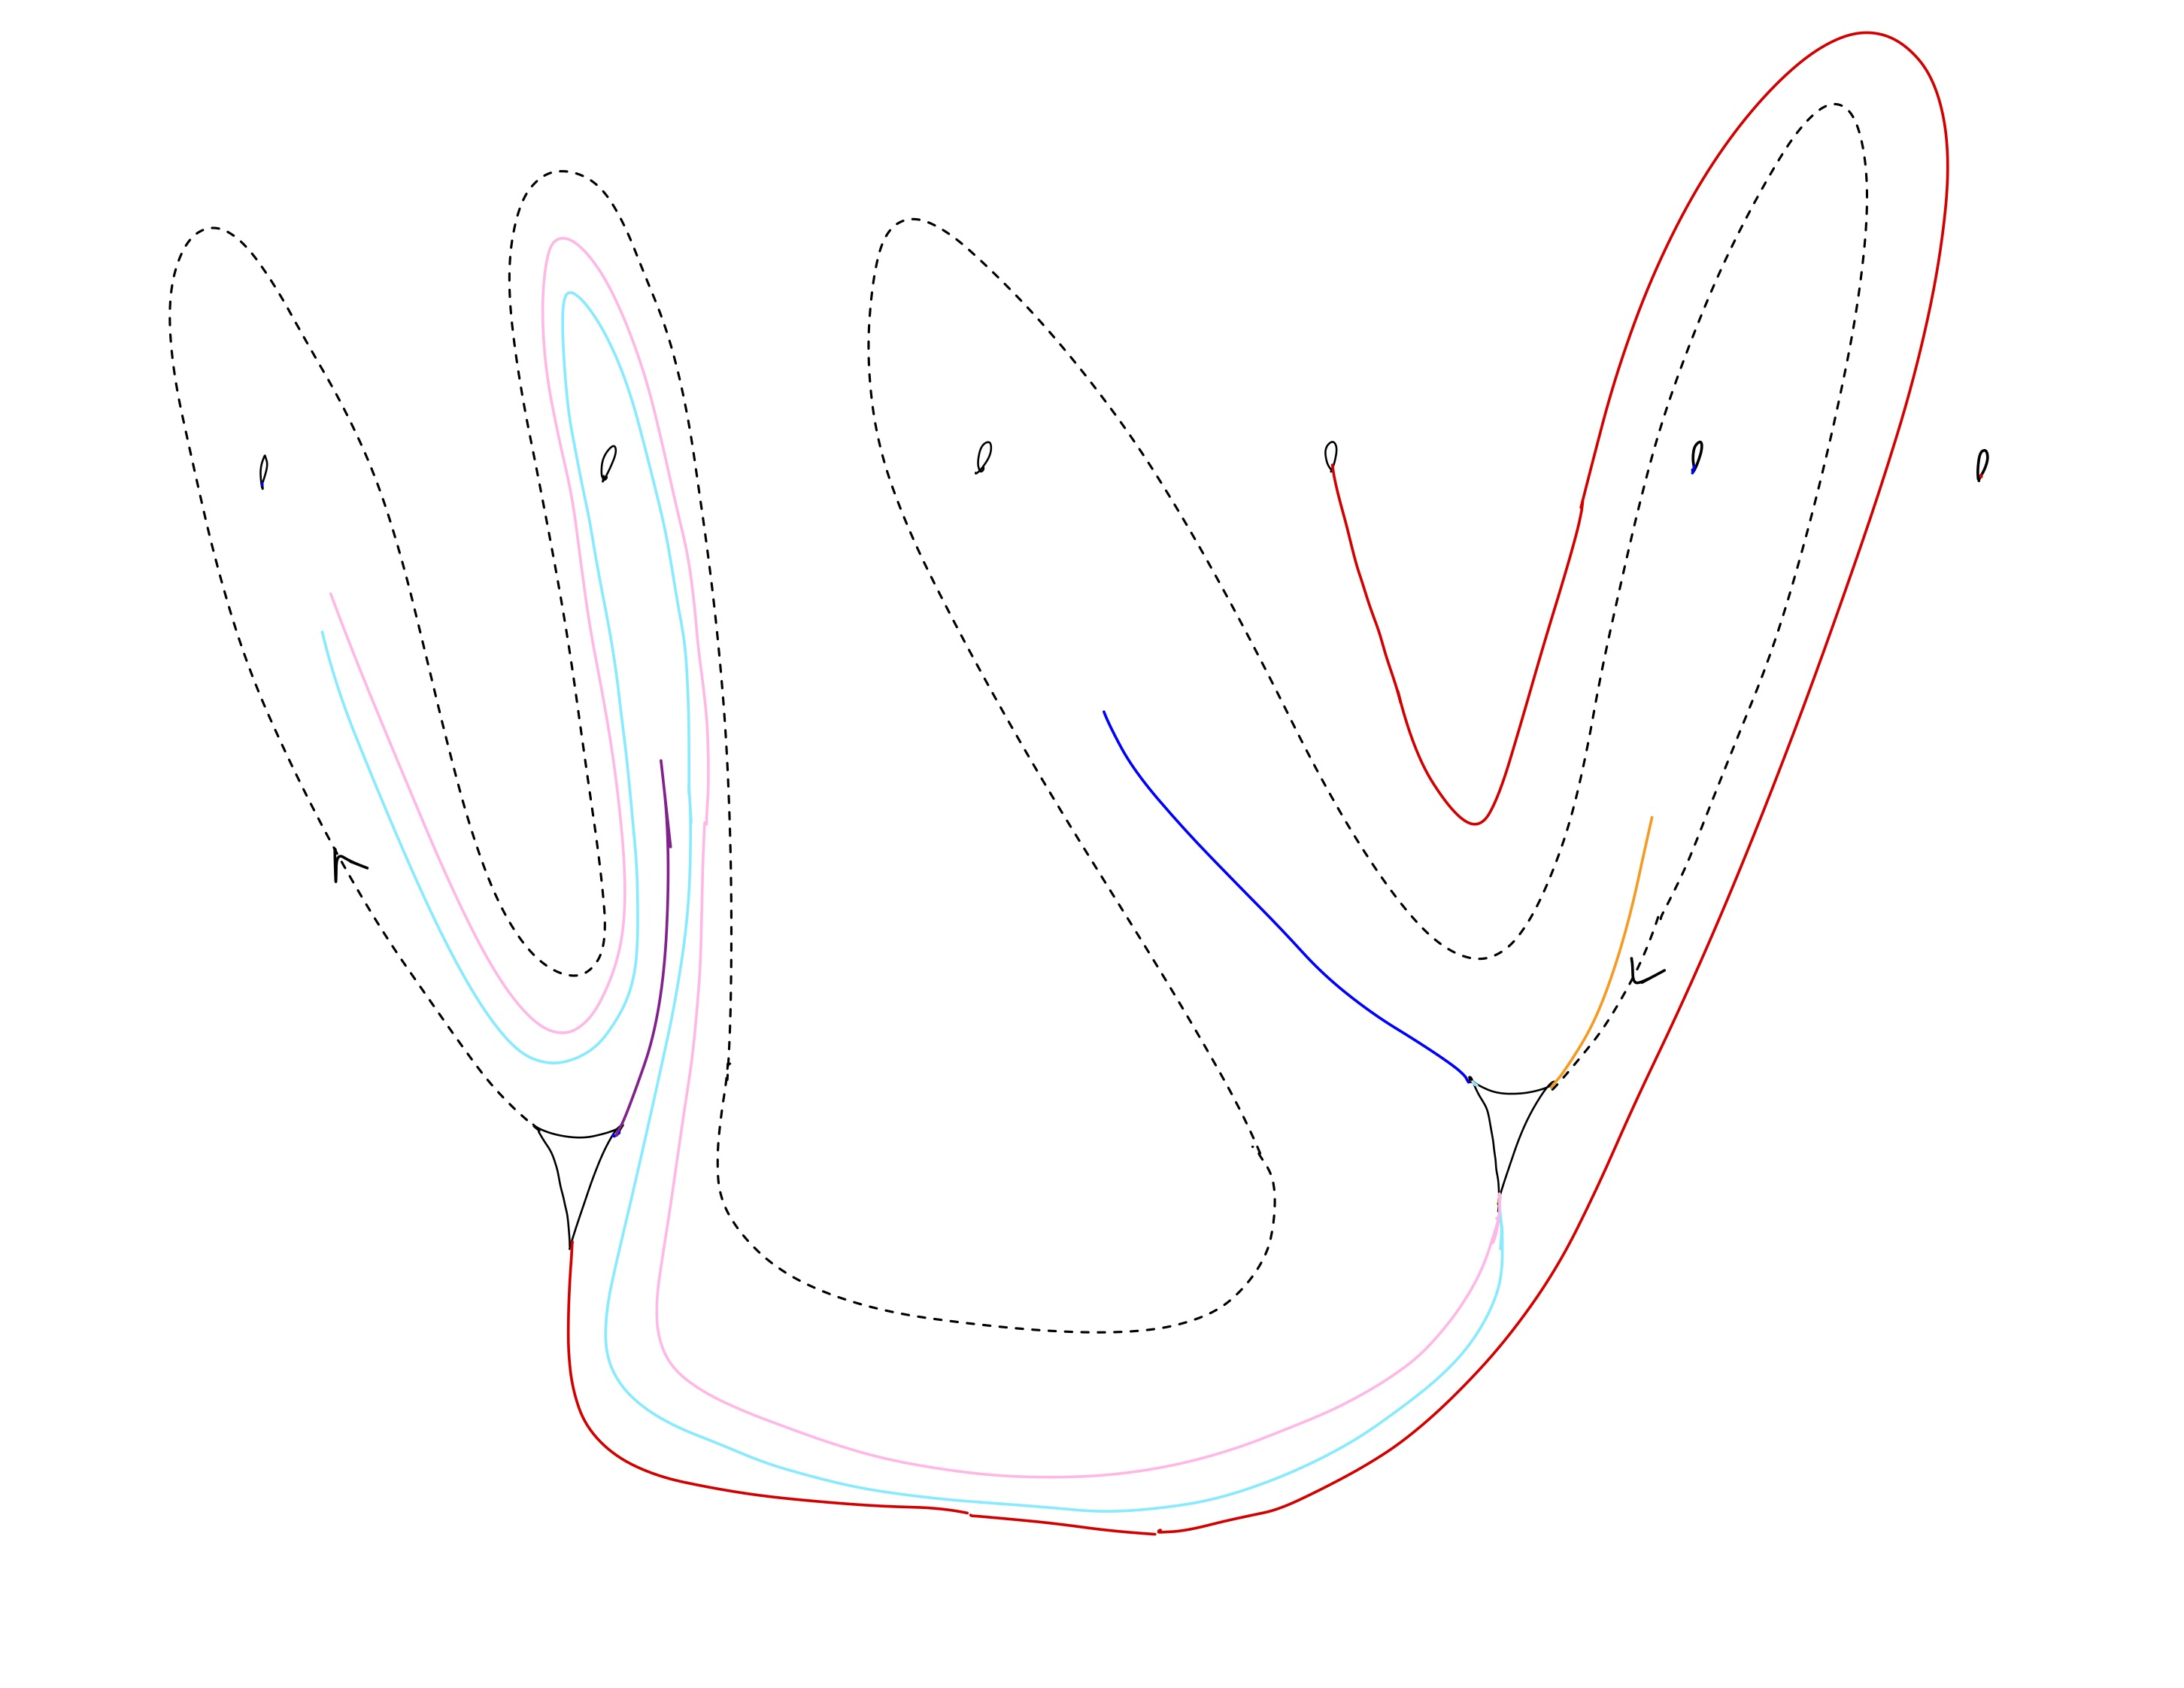
\includegraphics[width=\linewidth]{figures_case_analysis/track17_case_analysis/Moke-7.jpg}
    \caption{Moke7}
    \label{fig:Moke7}
\end{figure}

\begin{figure}[ht]
    \centering
    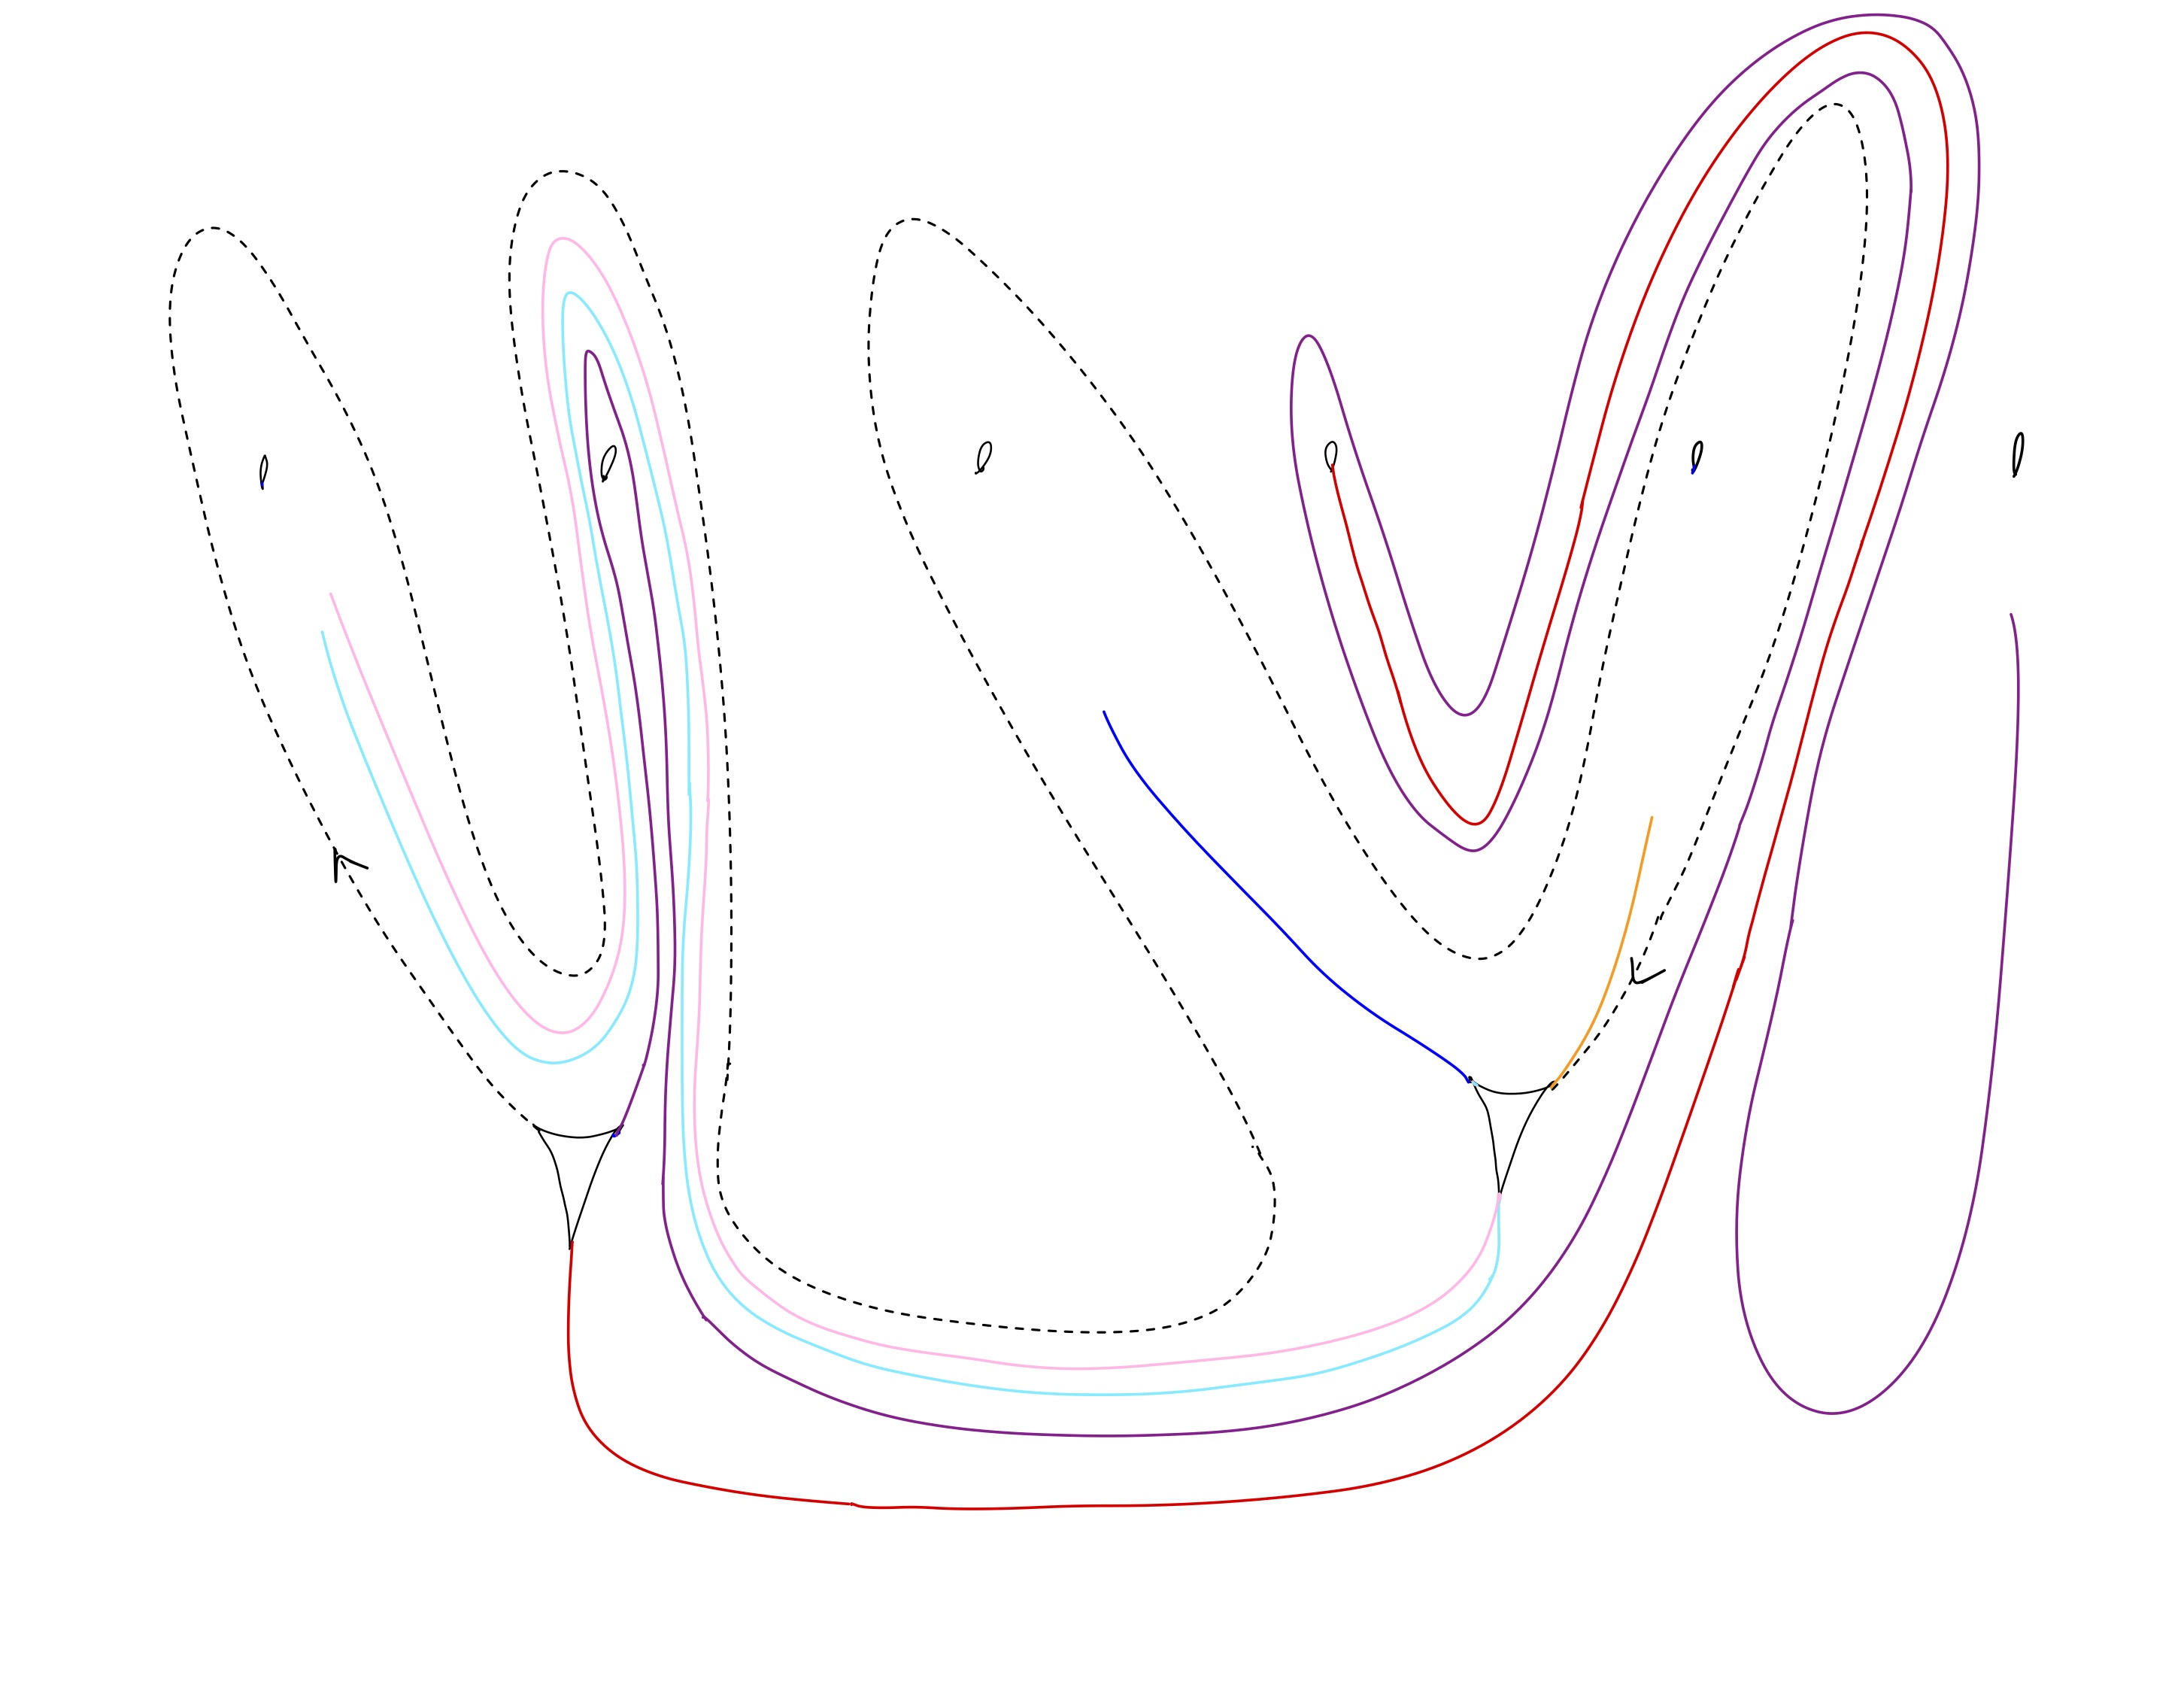
\includegraphics[width=\linewidth]{figures_case_analysis/track17_case_analysis/Moke-8.jpg}
    \caption{Moke8}
    \label{fig:Moke8}
\end{figure}

\begin{figure}[ht]
    \centering
    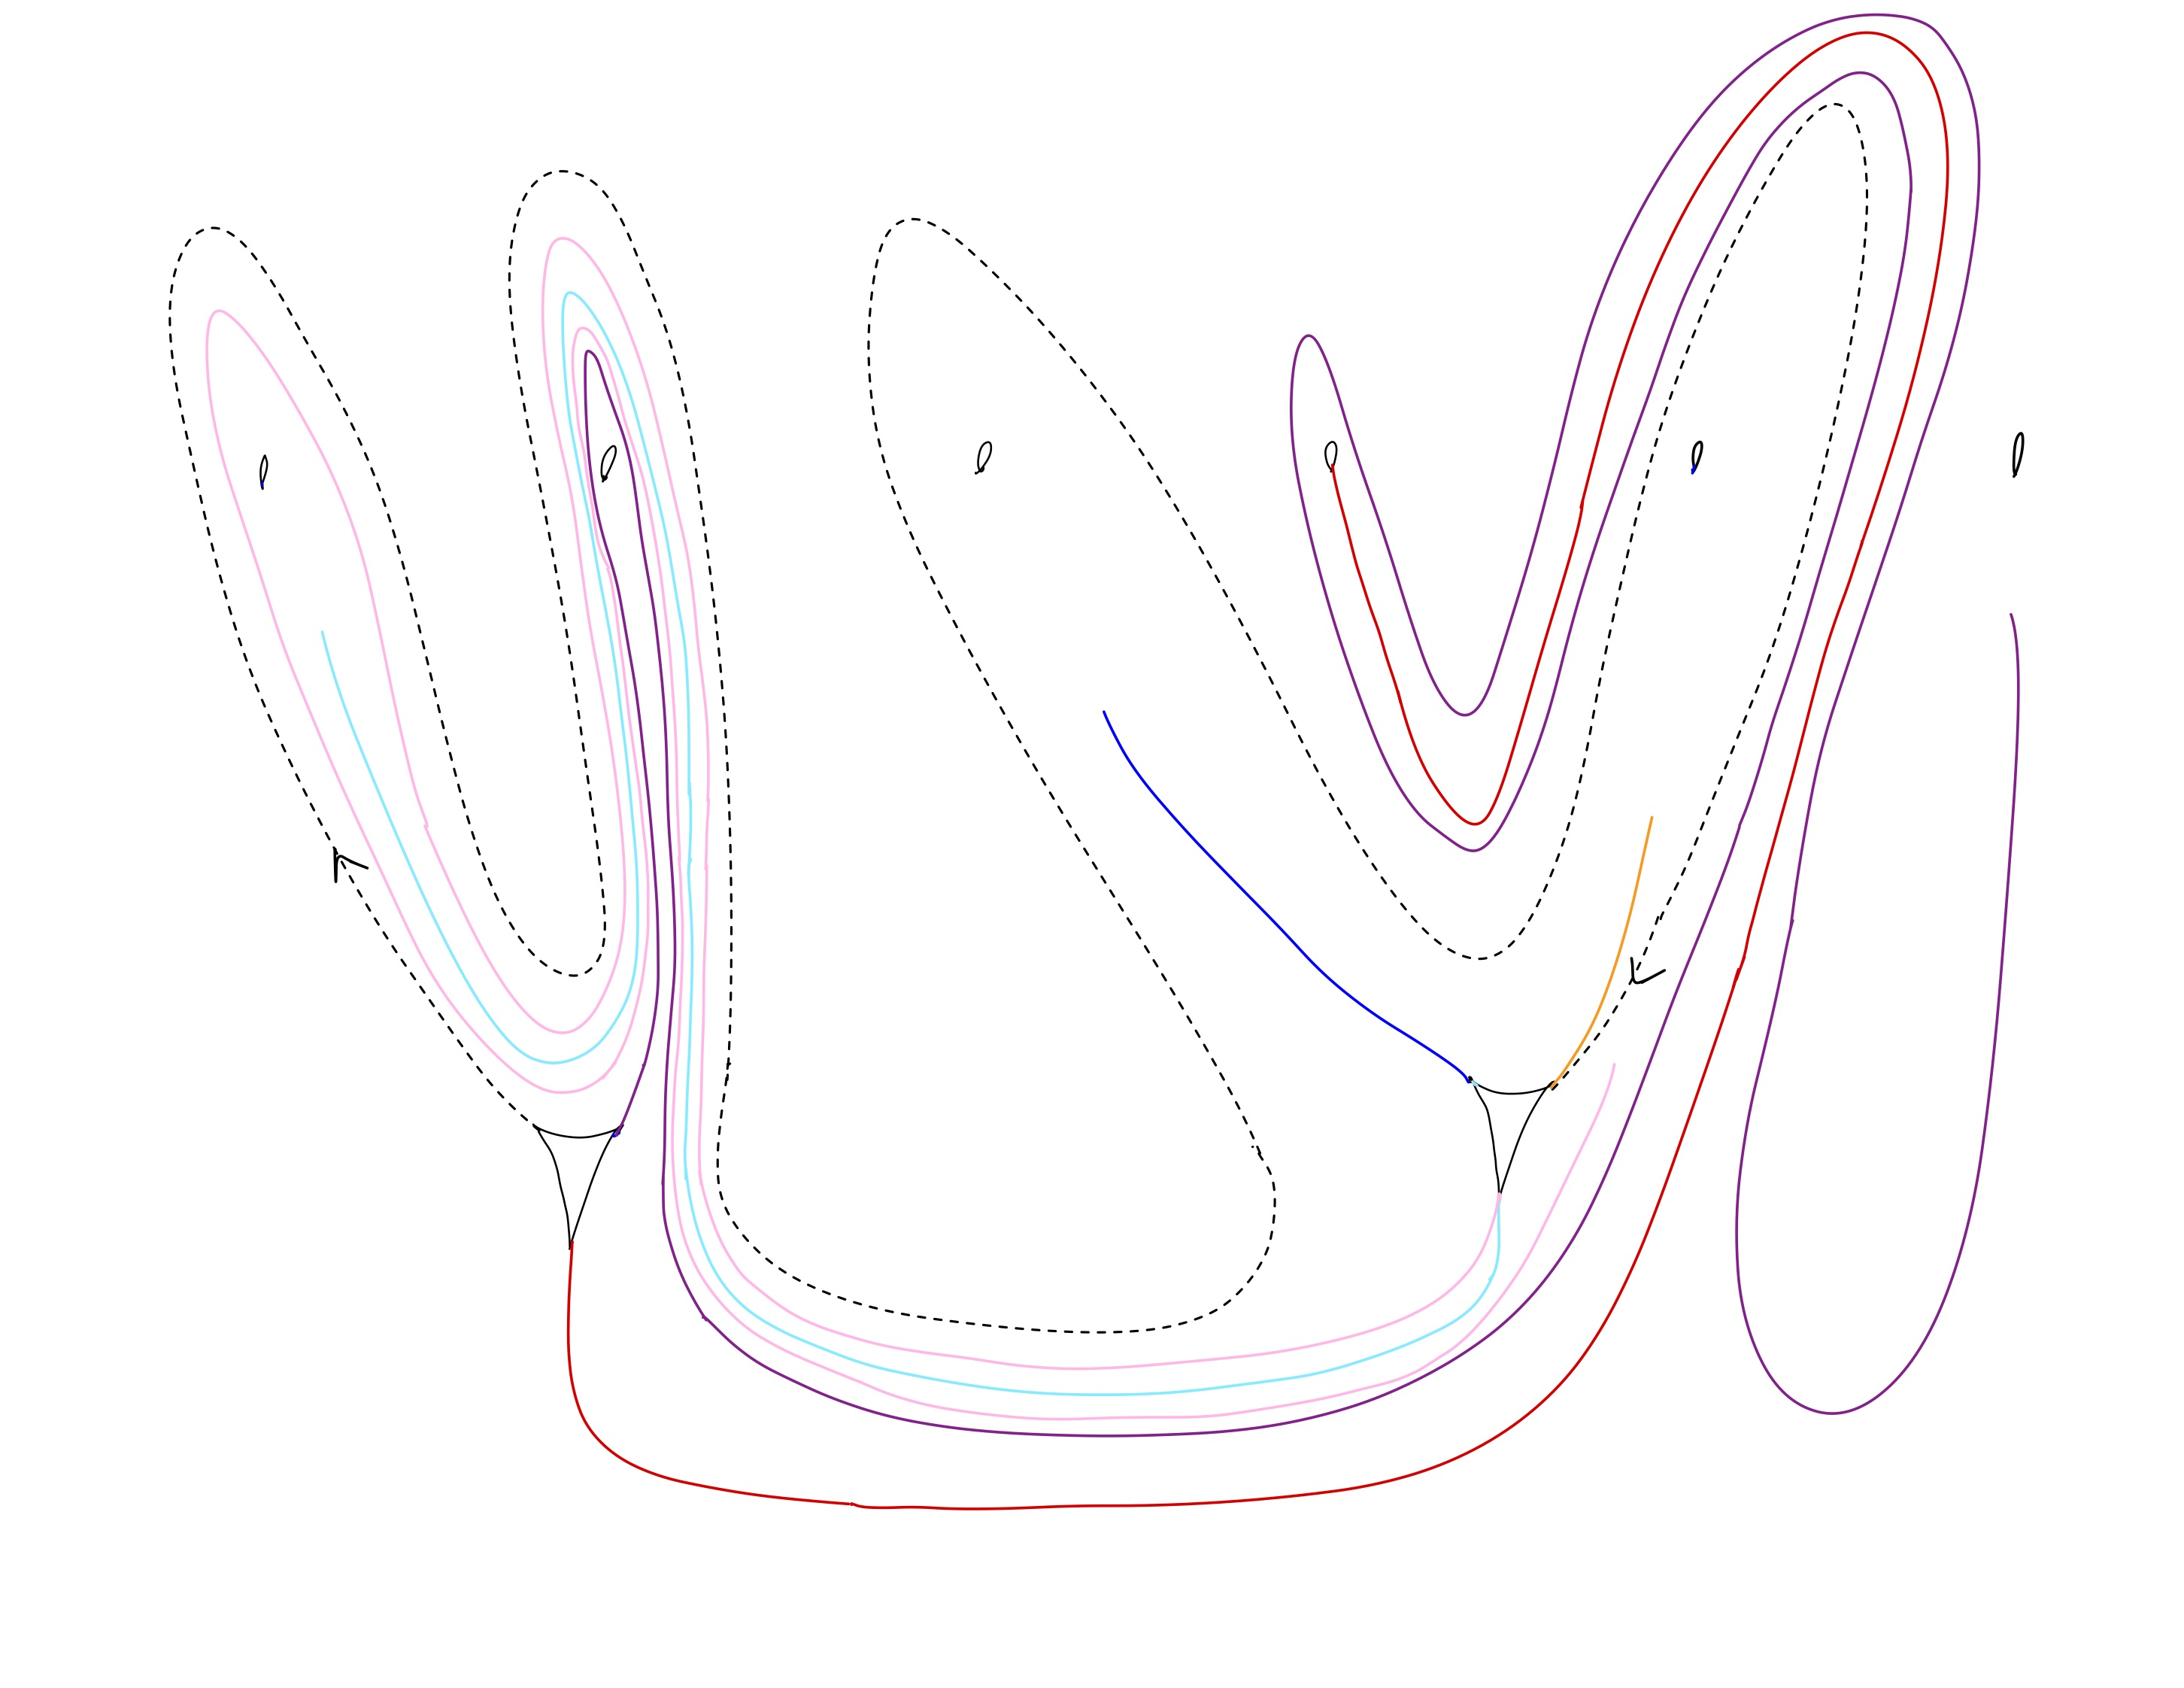
\includegraphics[width=\linewidth]{figures_case_analysis/track17_case_analysis/Moke-9.jpg}
    \caption{Moke9}
    \label{fig:Moke9}
\end{figure}

\begin{figure}[ht]
    \centering
    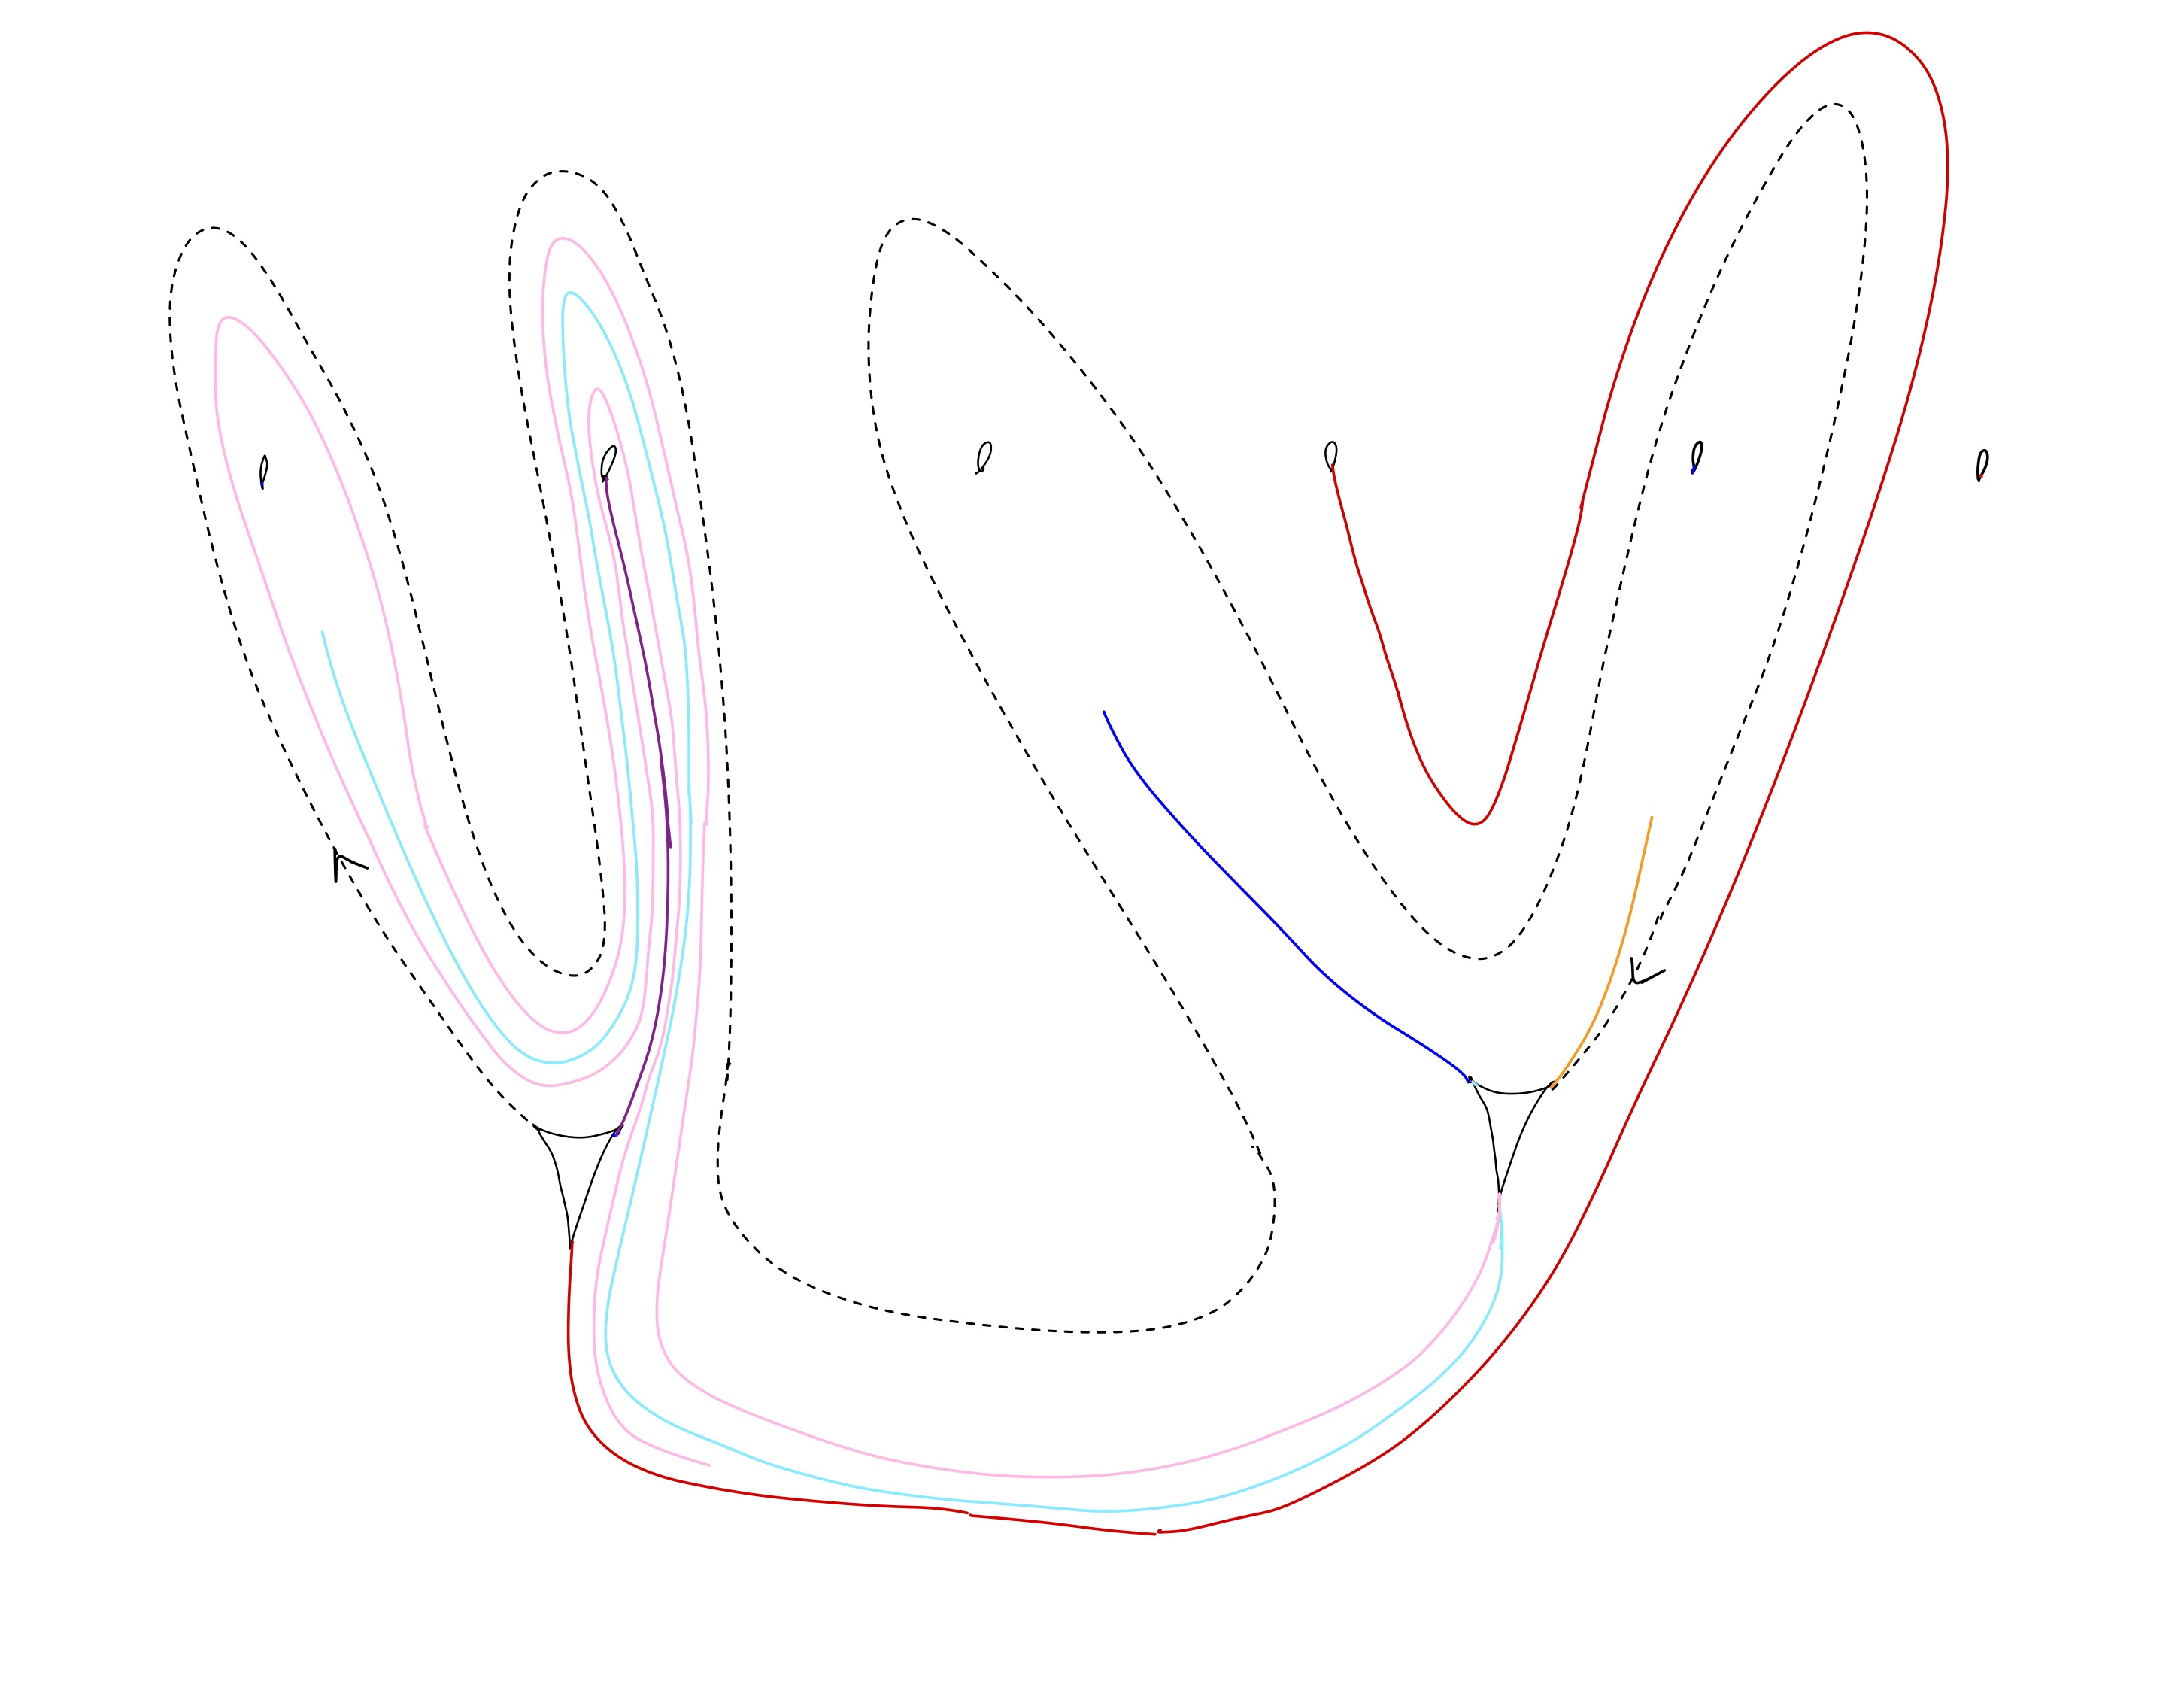
\includegraphics[width=\linewidth]{figures_case_analysis/track17_case_analysis/Moke-10.jpg}
    \caption{Moke10}
    \label{fig:Moke10}
\end{figure}
\clearpage

\begin{figure}[ht]
    \centering
    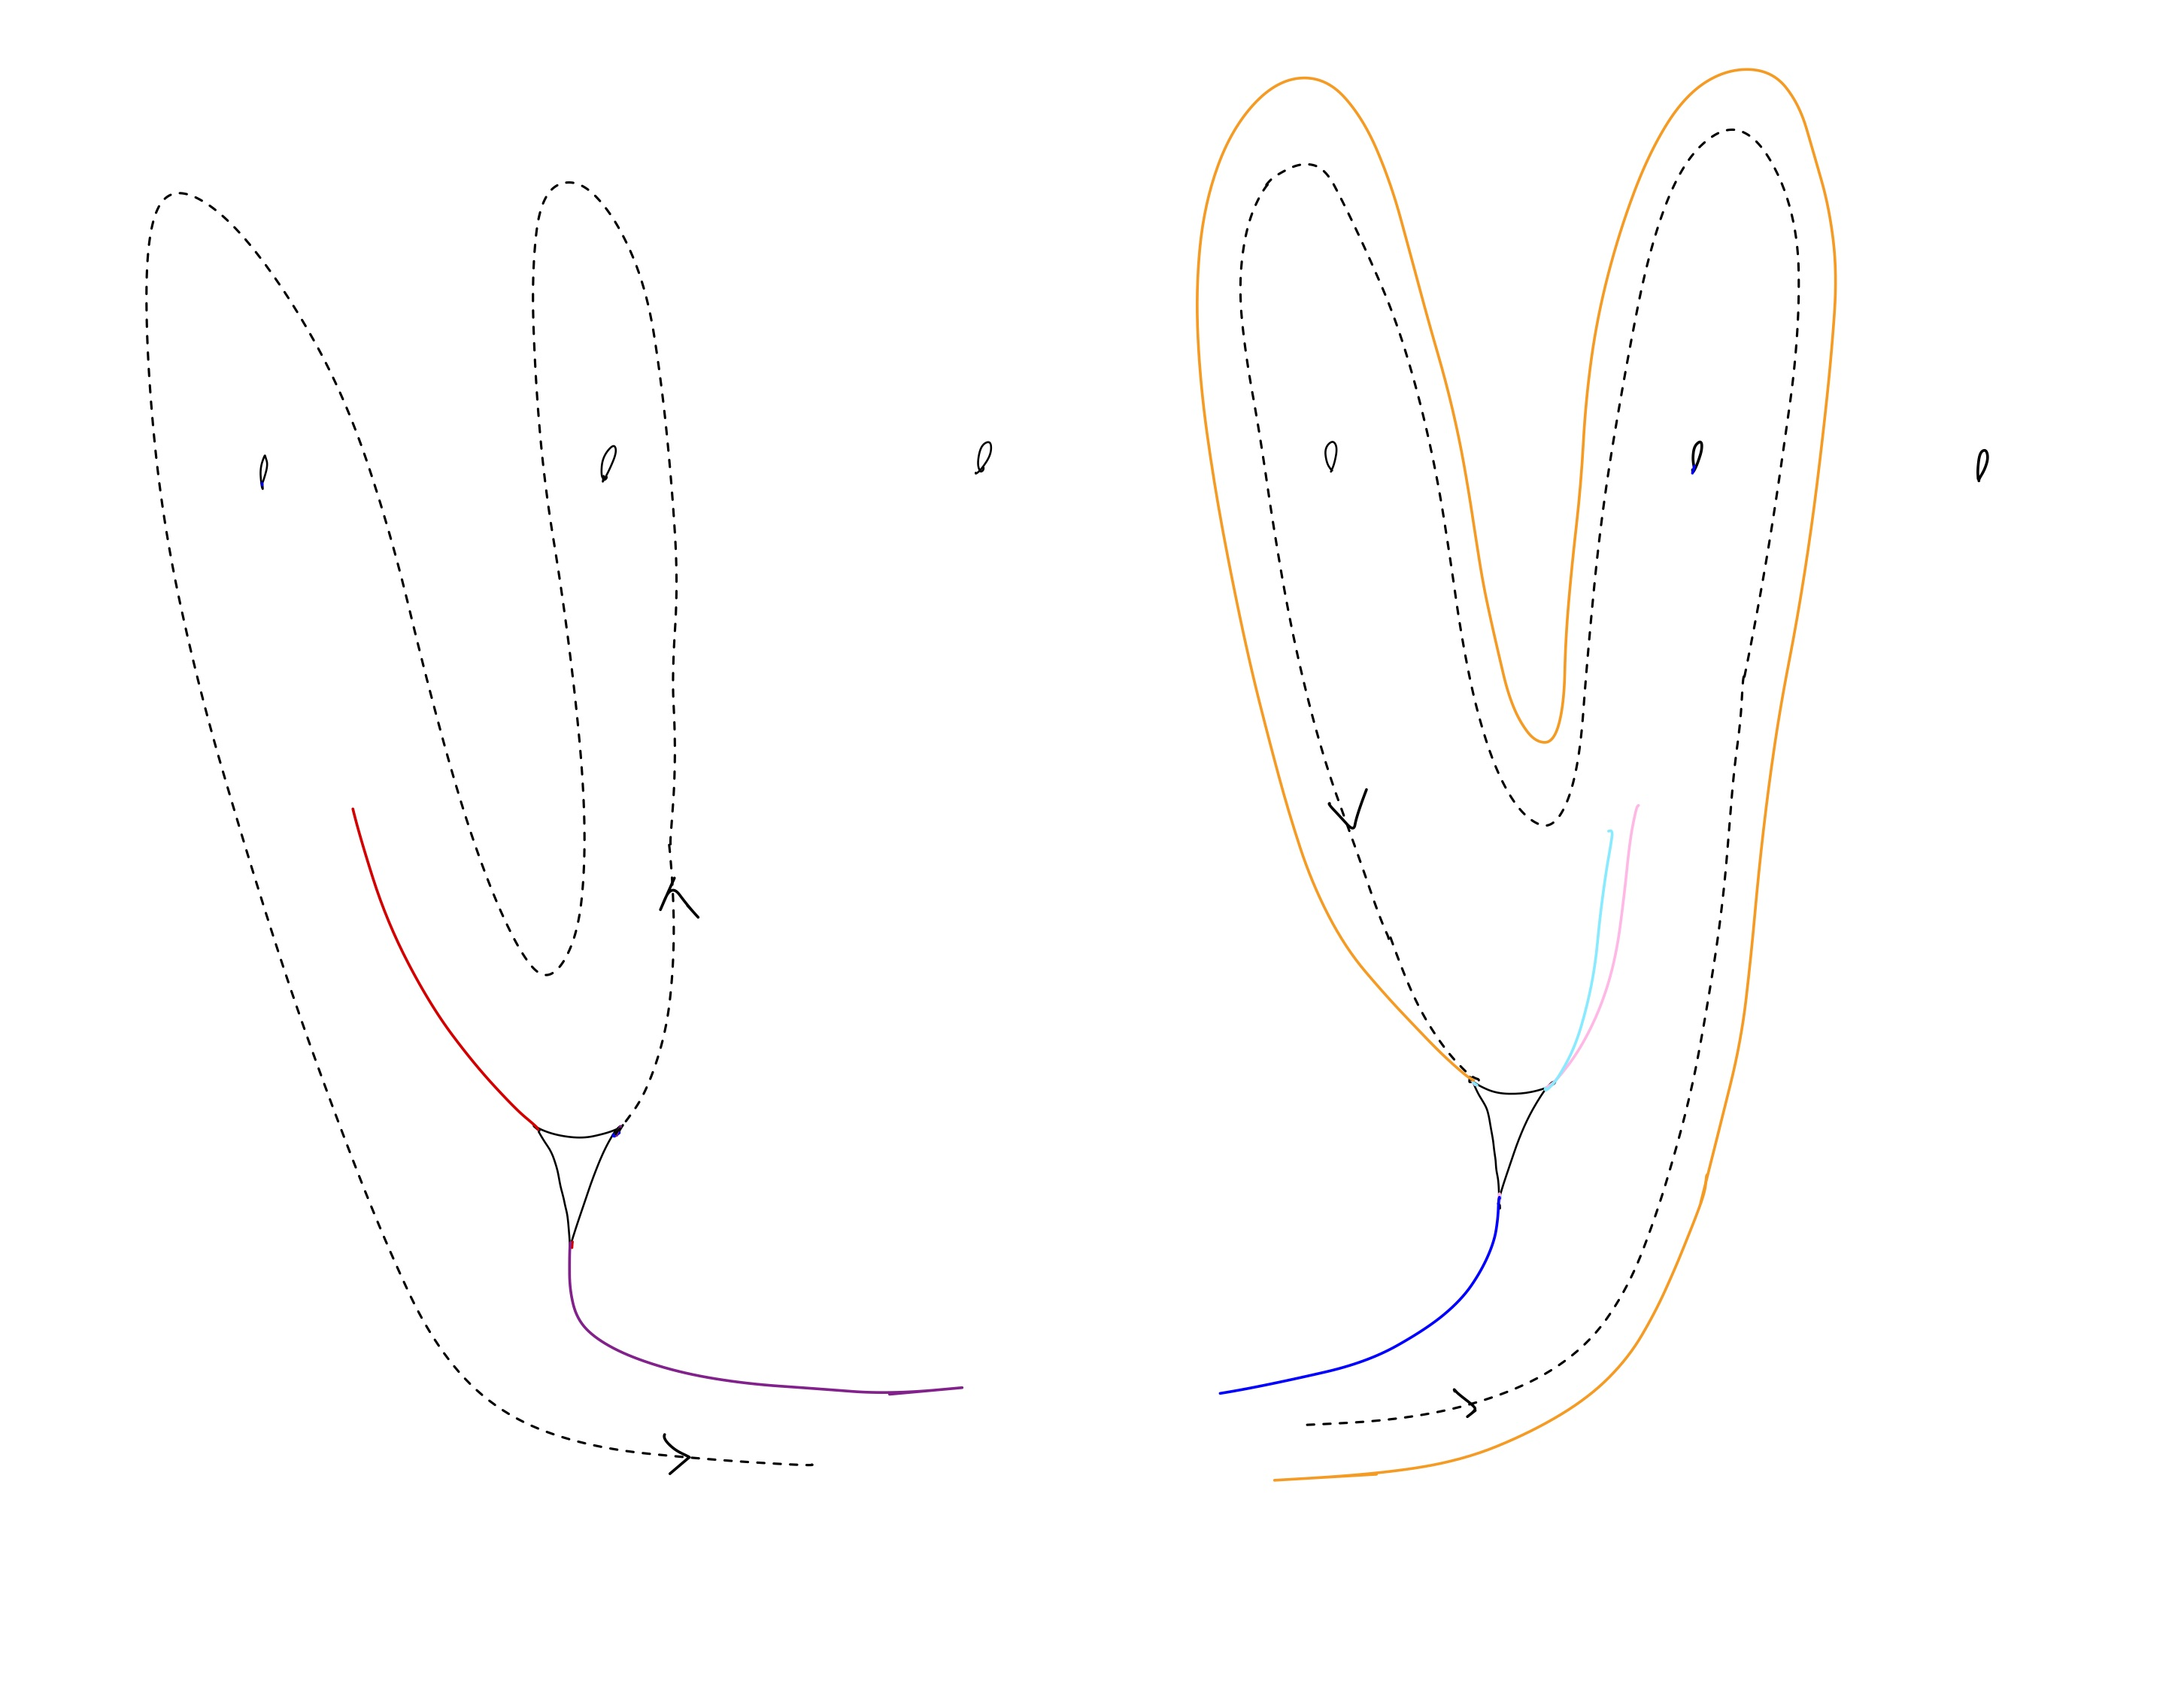
\includegraphics[width=\linewidth]{figures_case_analysis/track17_case_analysis/UAH-1.jpg}
    \caption{UAH1}
    \label{fig:UAH1}
\end{figure}

\begin{figure}[ht]
    \centering
    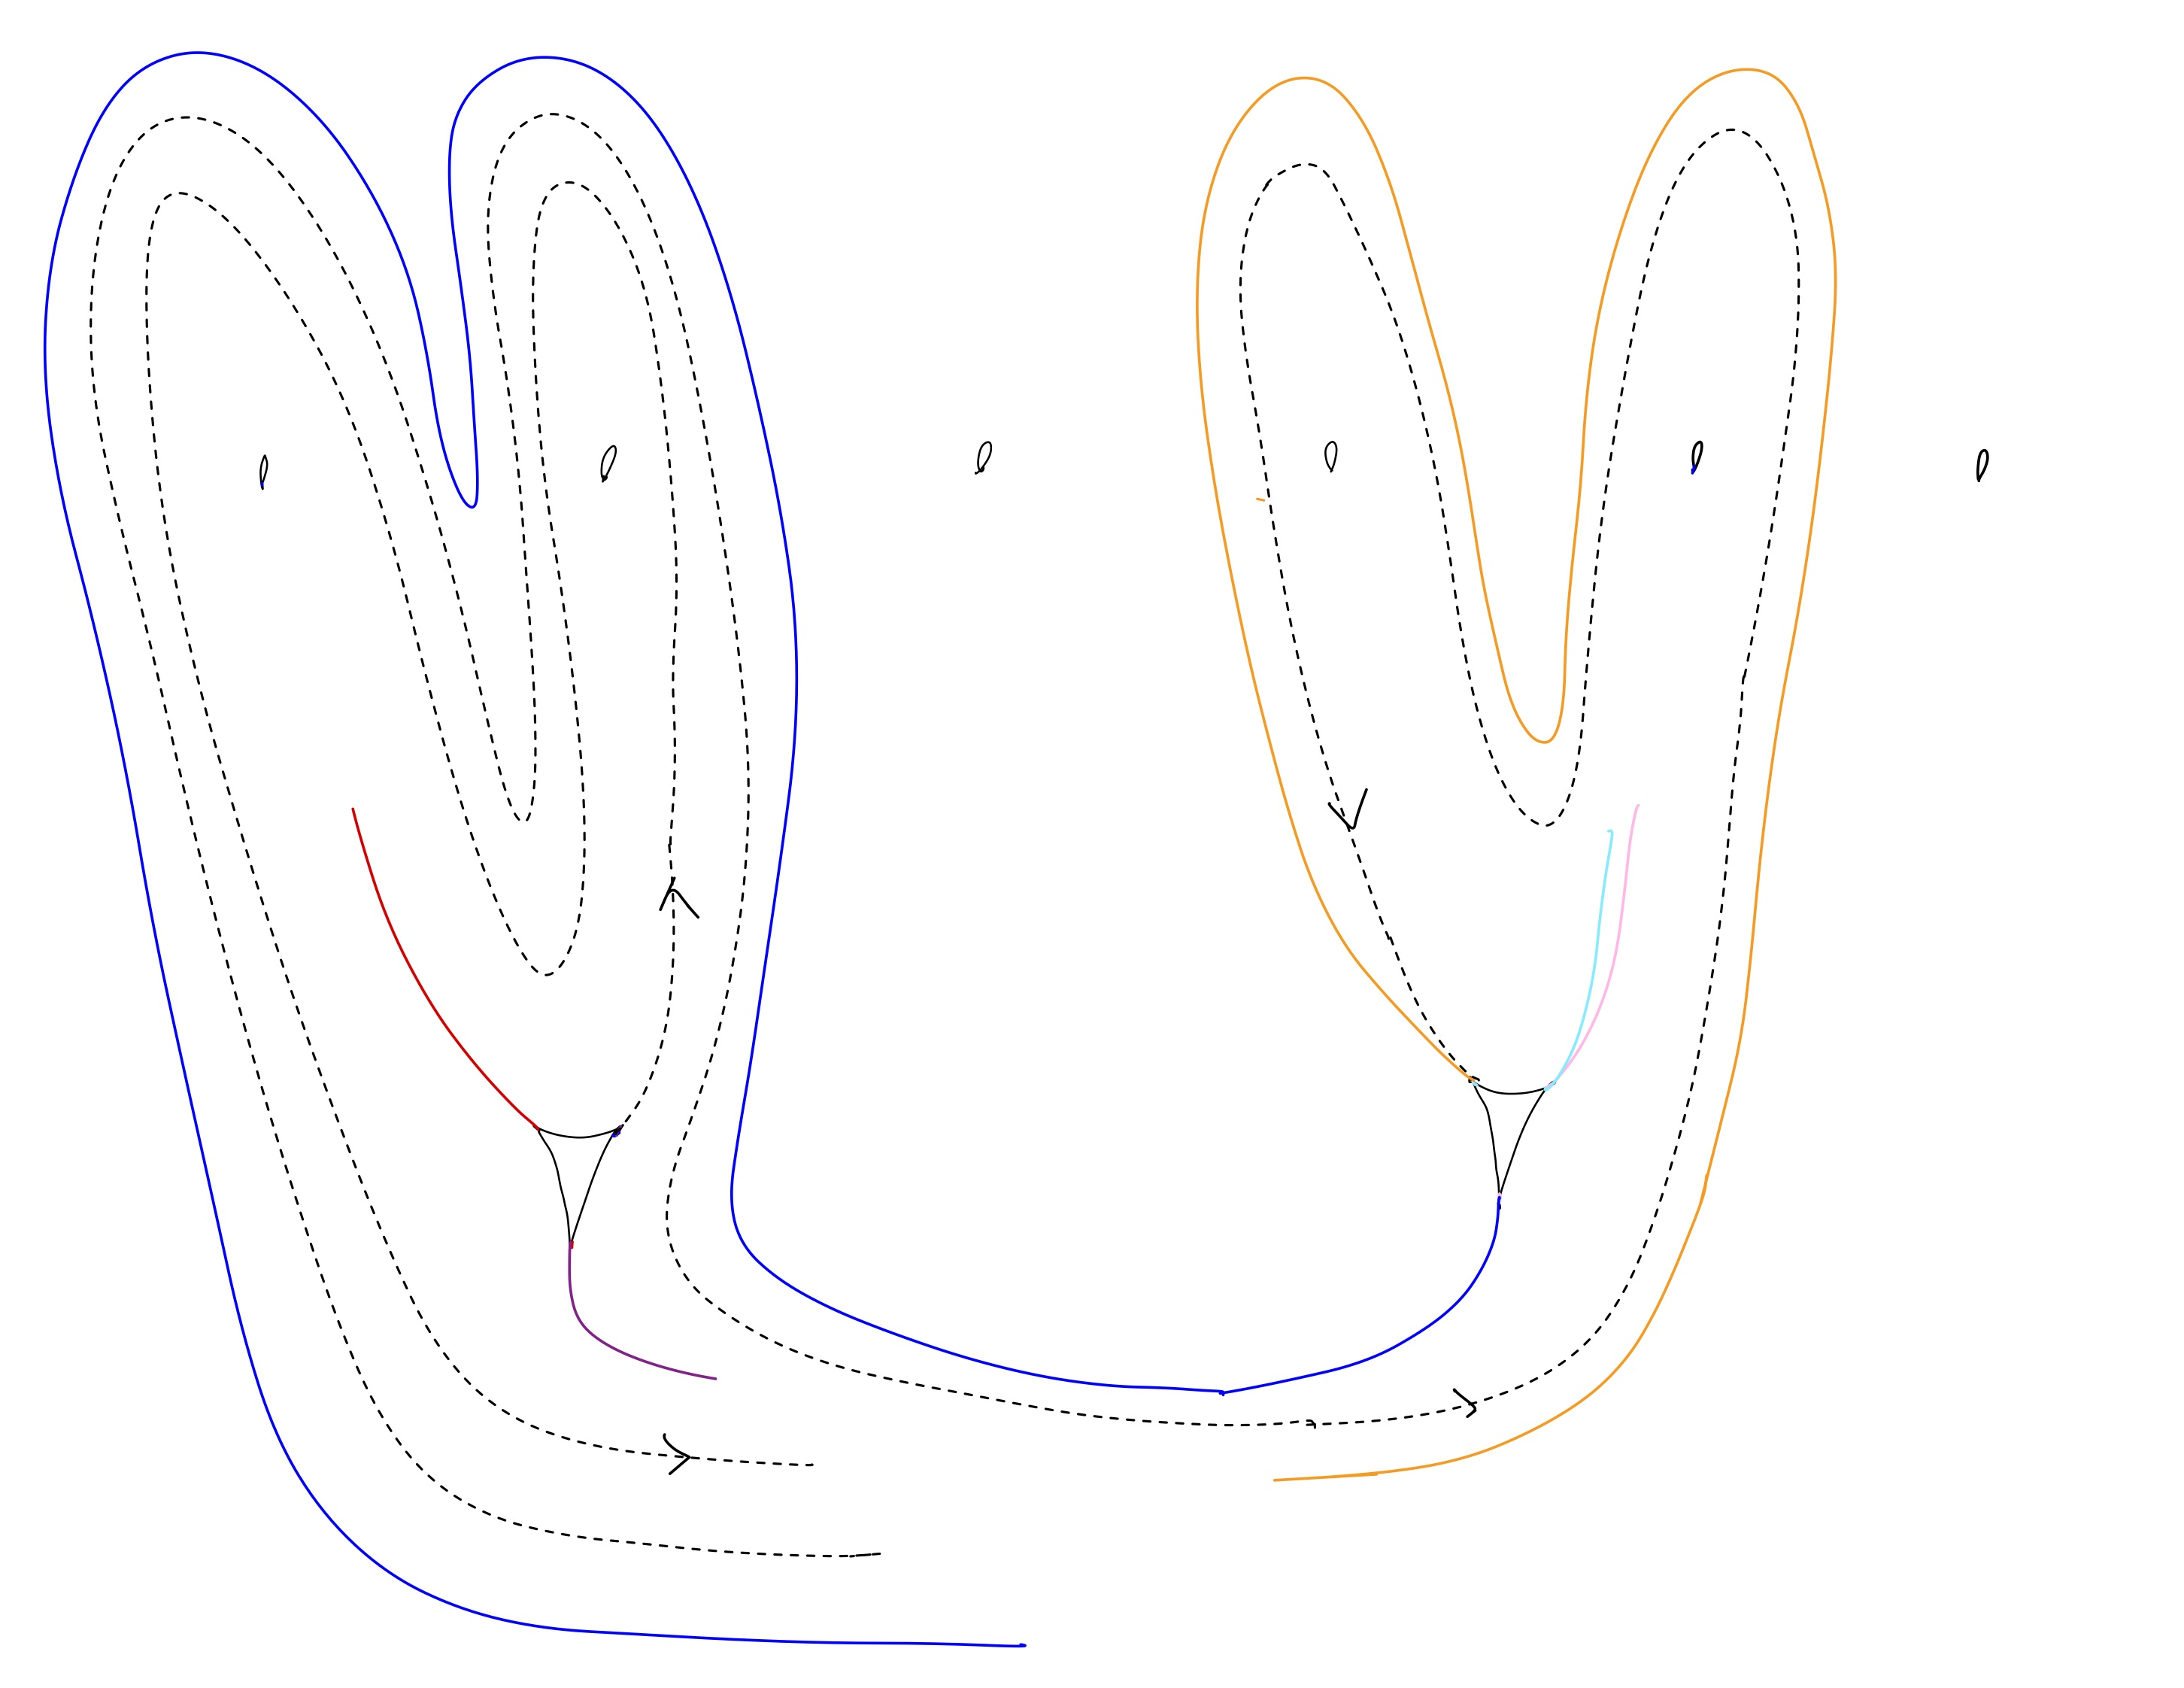
\includegraphics[width=\linewidth]{figures_case_analysis/track17_case_analysis/UAH-2.jpg}
    \caption{UAH2}
    \label{fig:UAH2}
\end{figure}

\begin{figure}[ht]
    \centering
    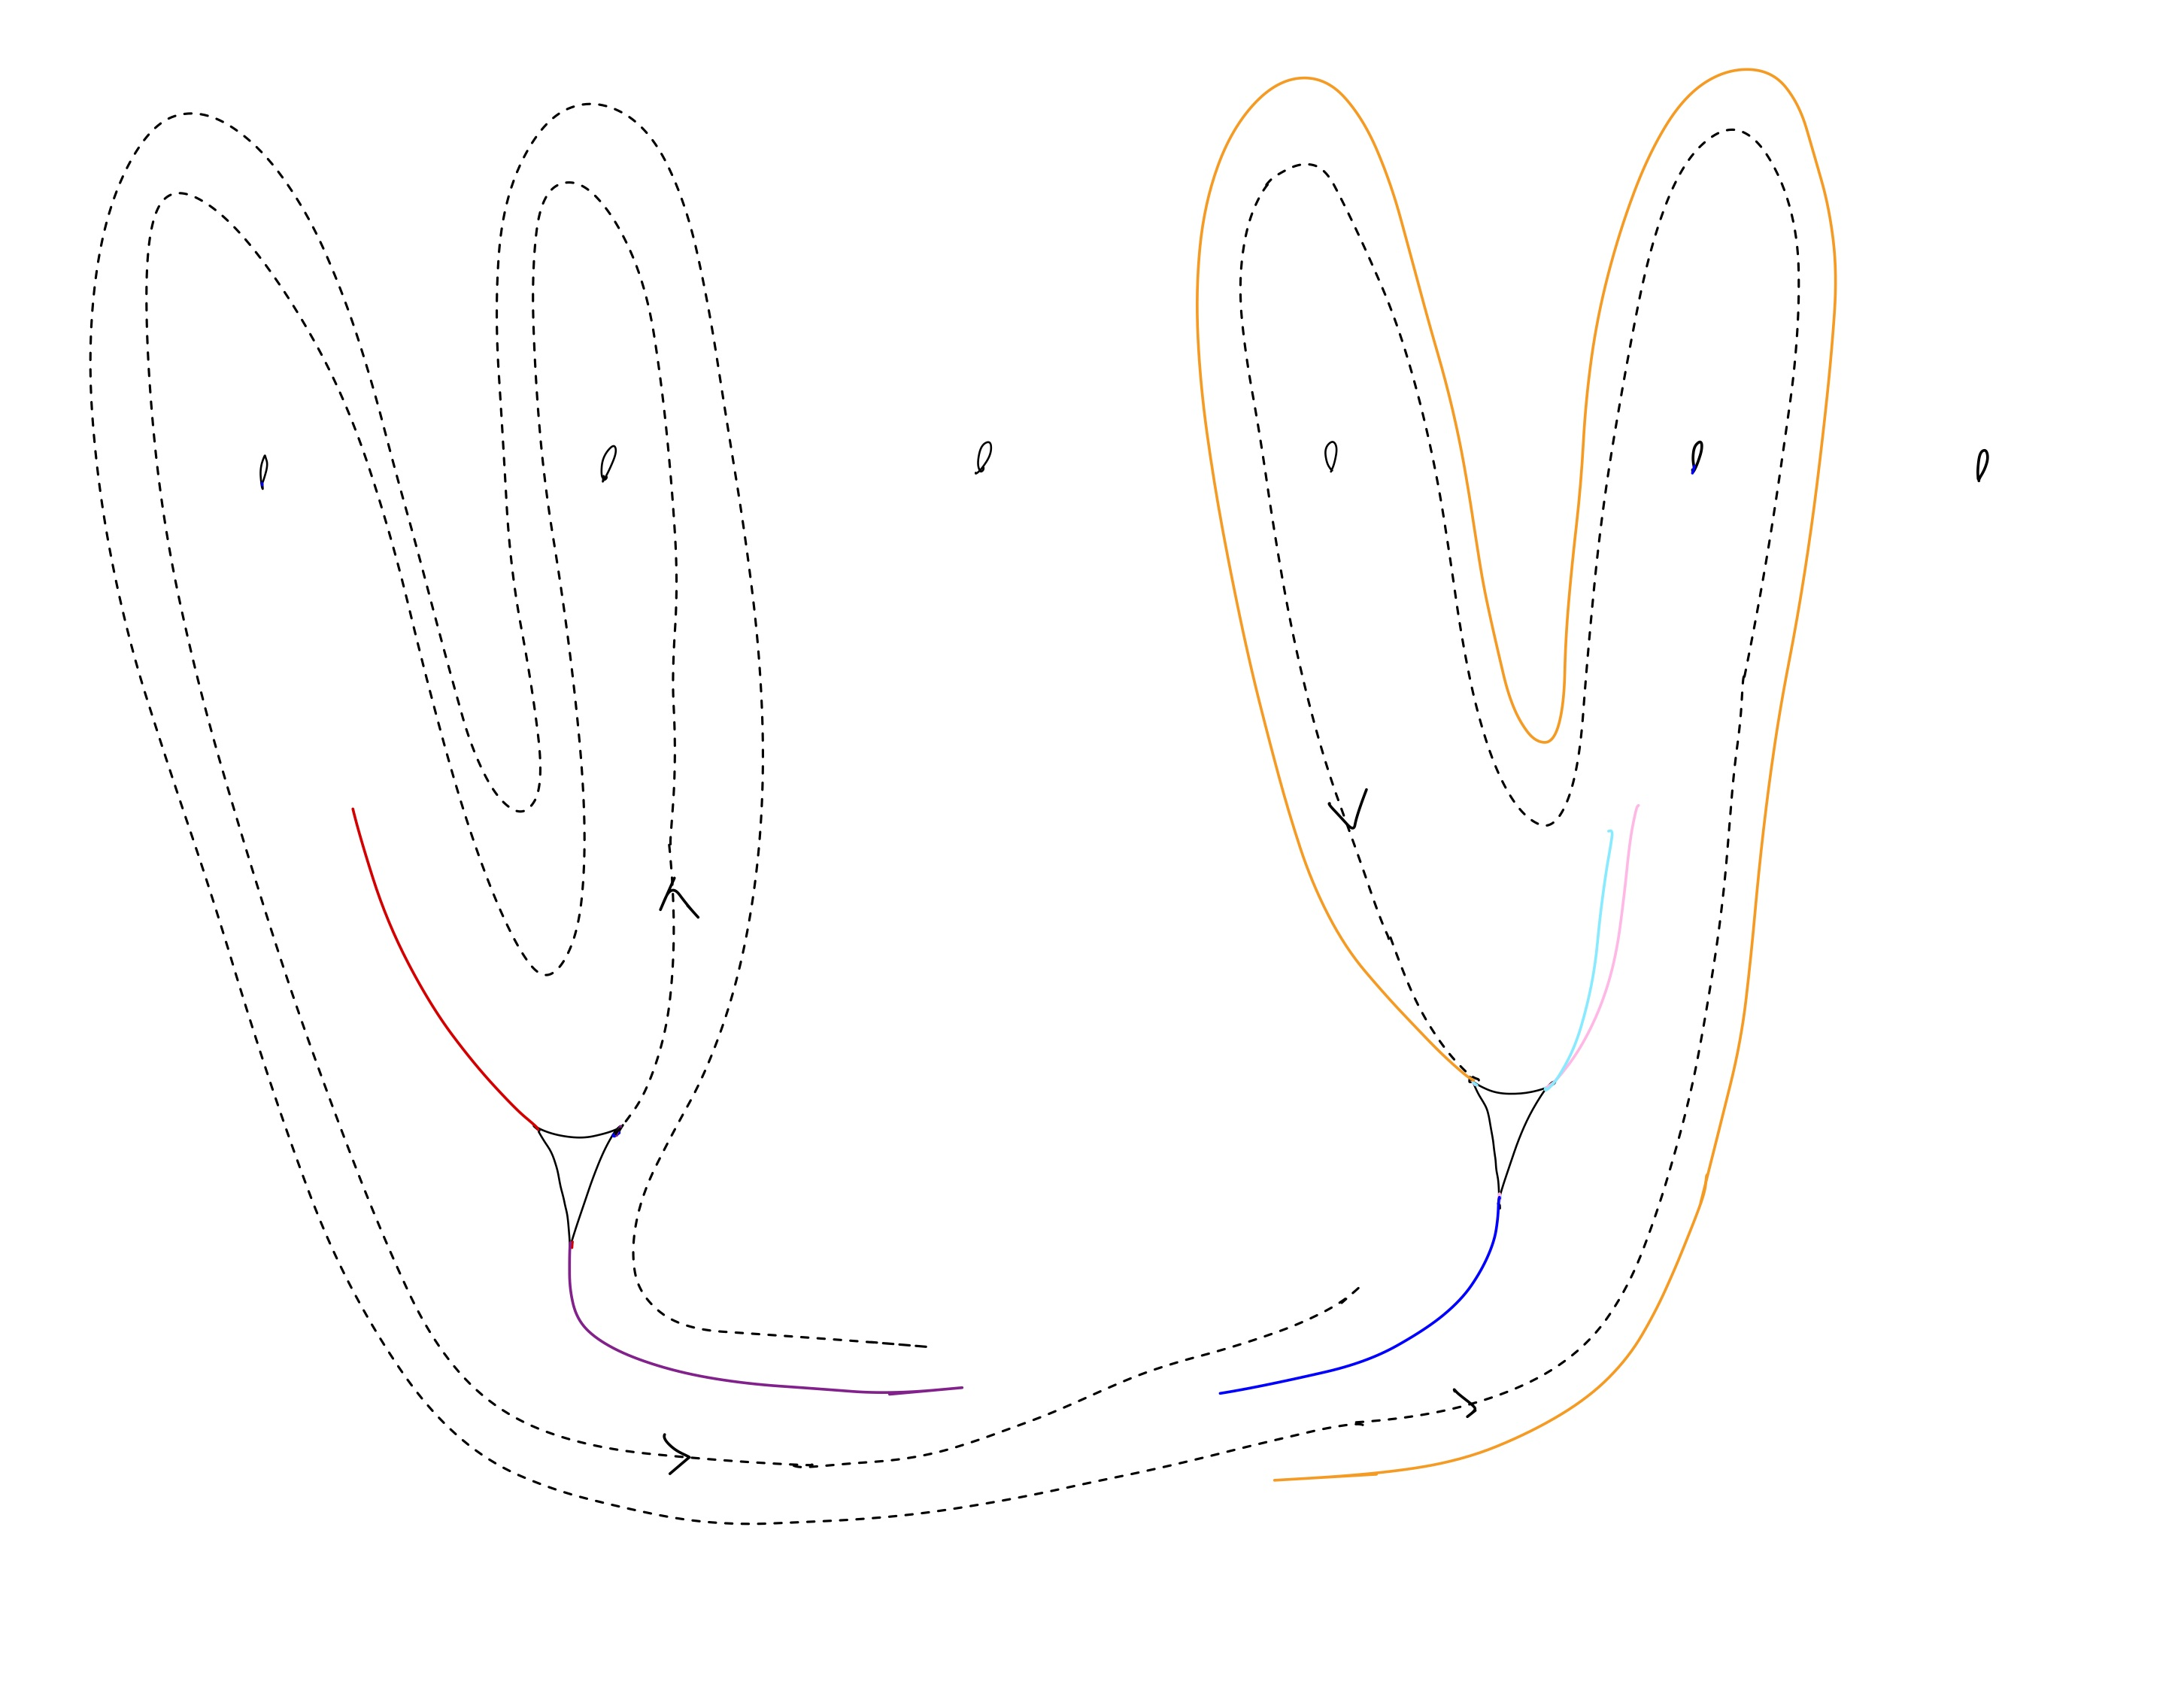
\includegraphics[width=\linewidth]{figures_case_analysis/track17_case_analysis/UAH-3.jpg}
    \caption{UAH3}
    \label{fig:UAH3}
\end{figure}

\begin{figure}[ht]
    \centering
    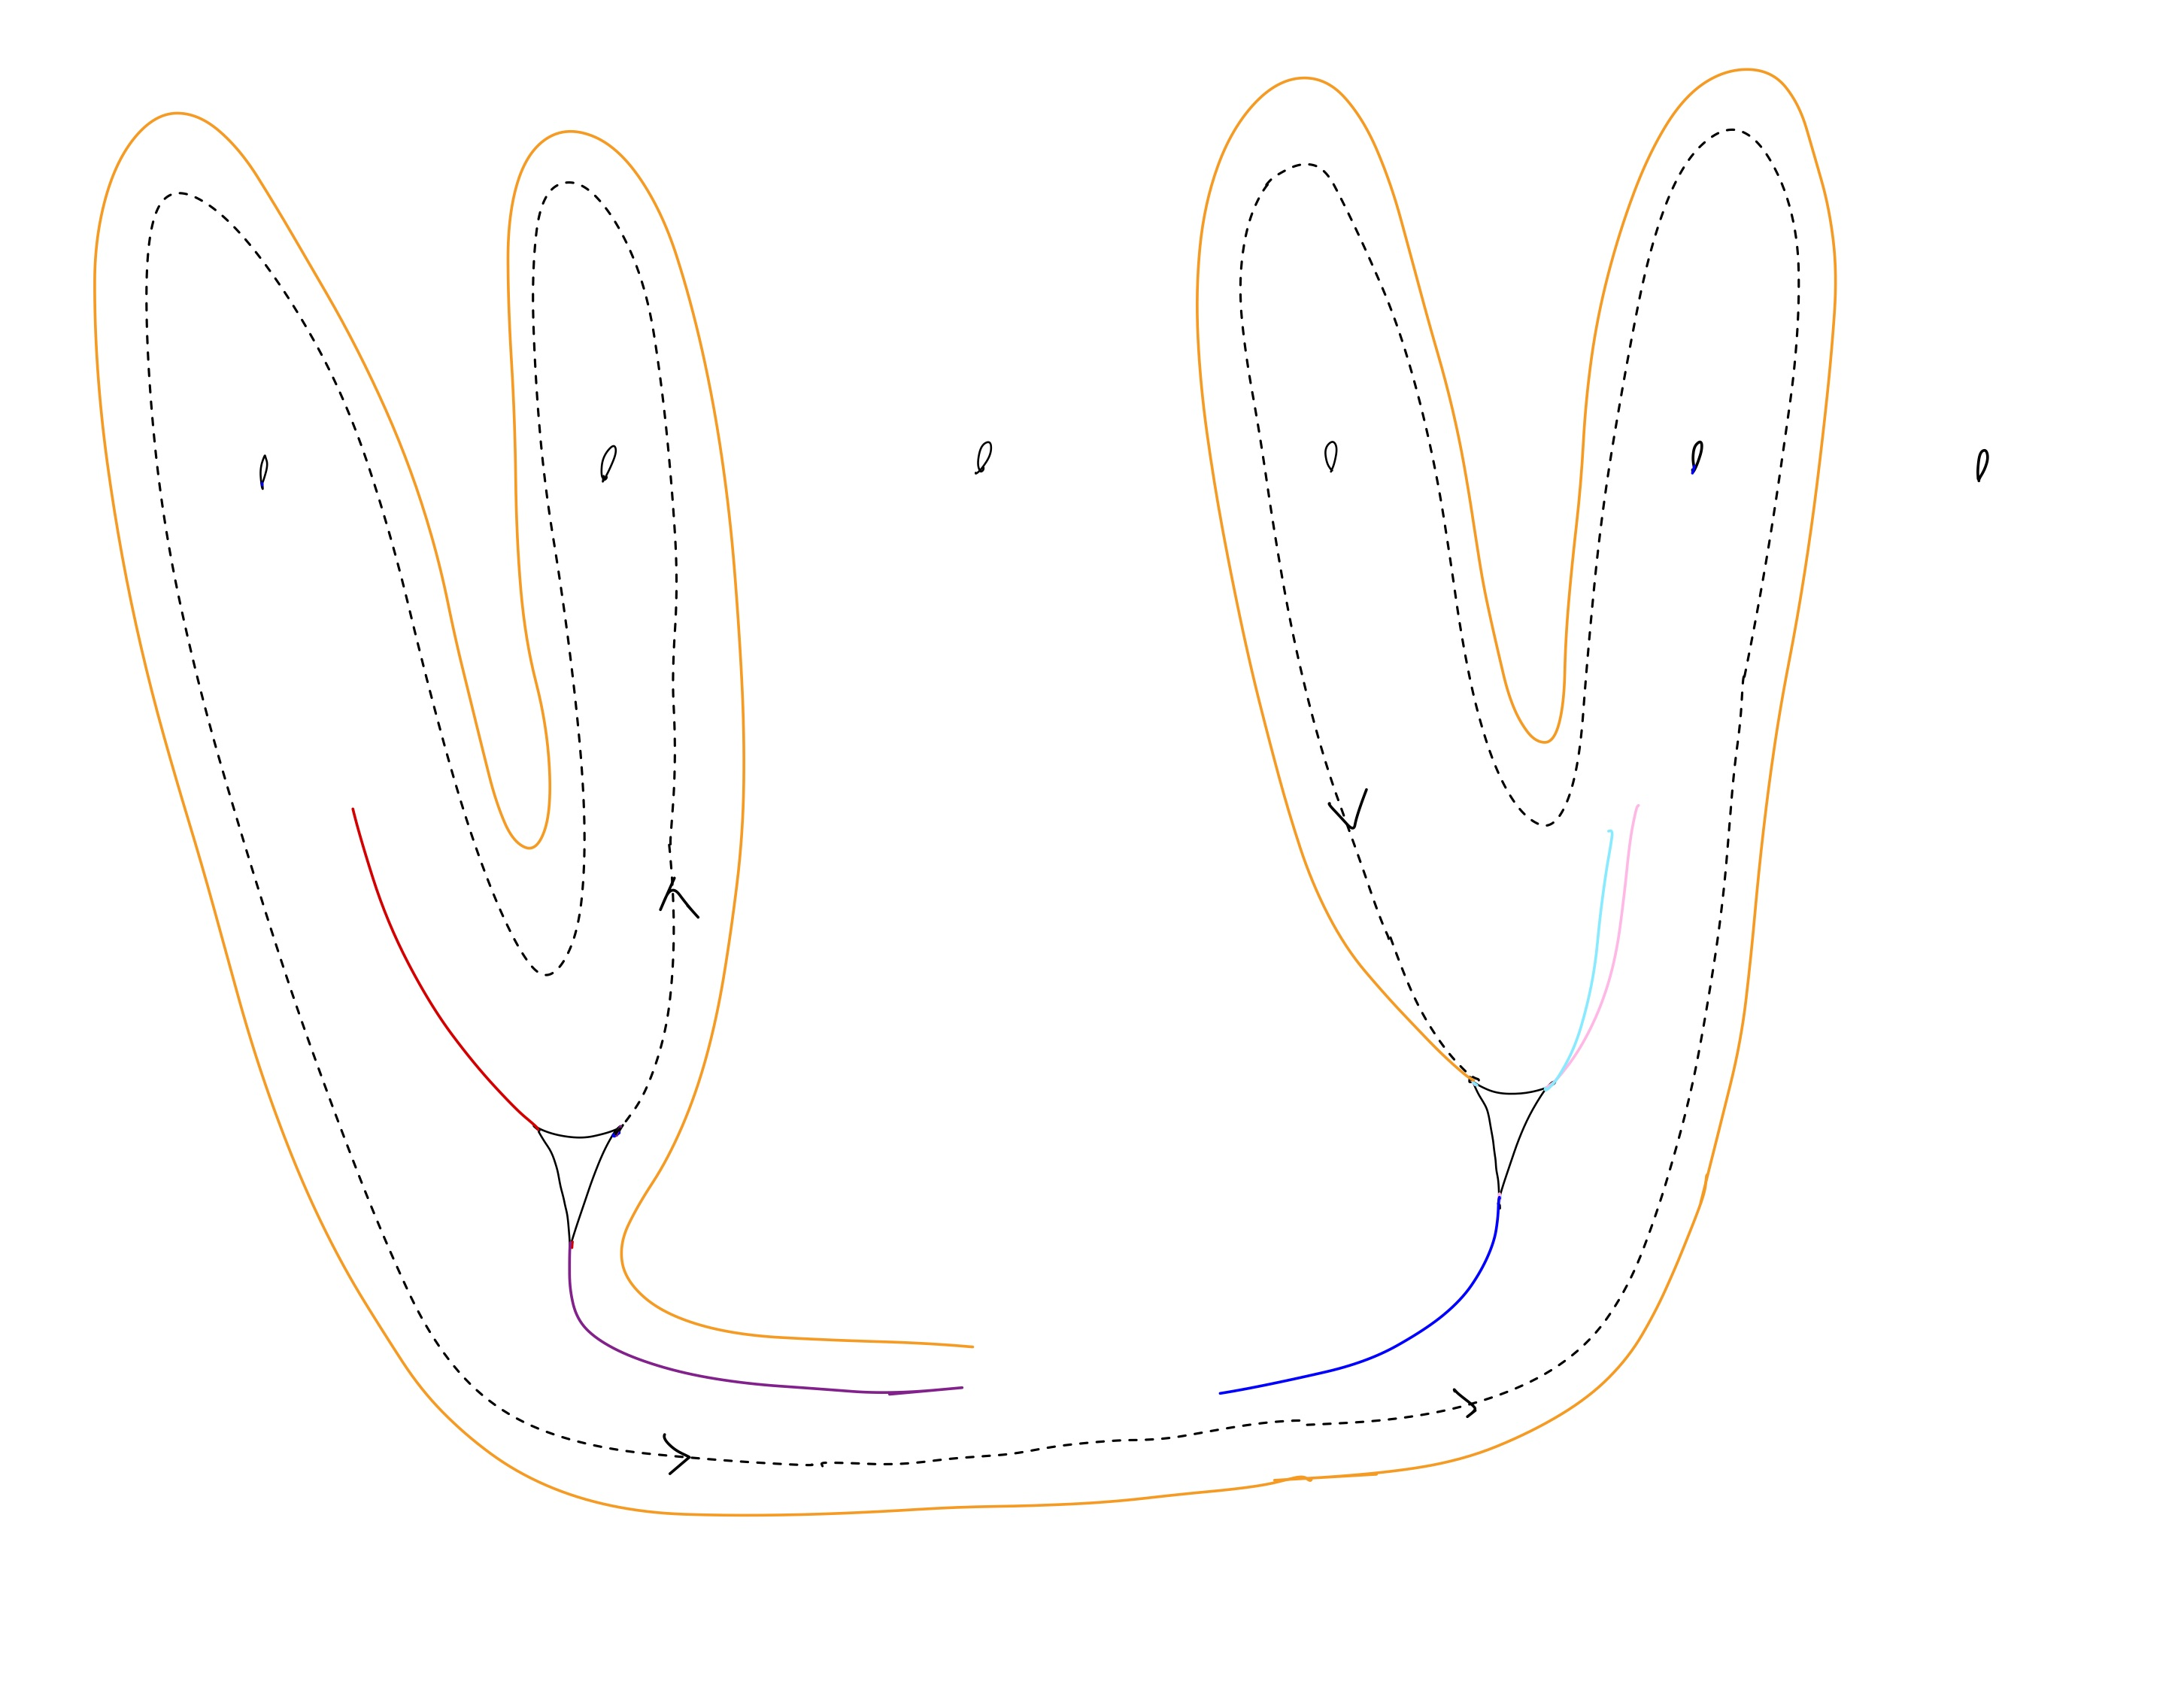
\includegraphics[width=\linewidth]{figures_case_analysis/track17_case_analysis/UAH-4.jpg}
    \caption{UAH4}
    \label{fig:UAH4}
\end{figure}

\begin{figure}[ht]
    \centering
    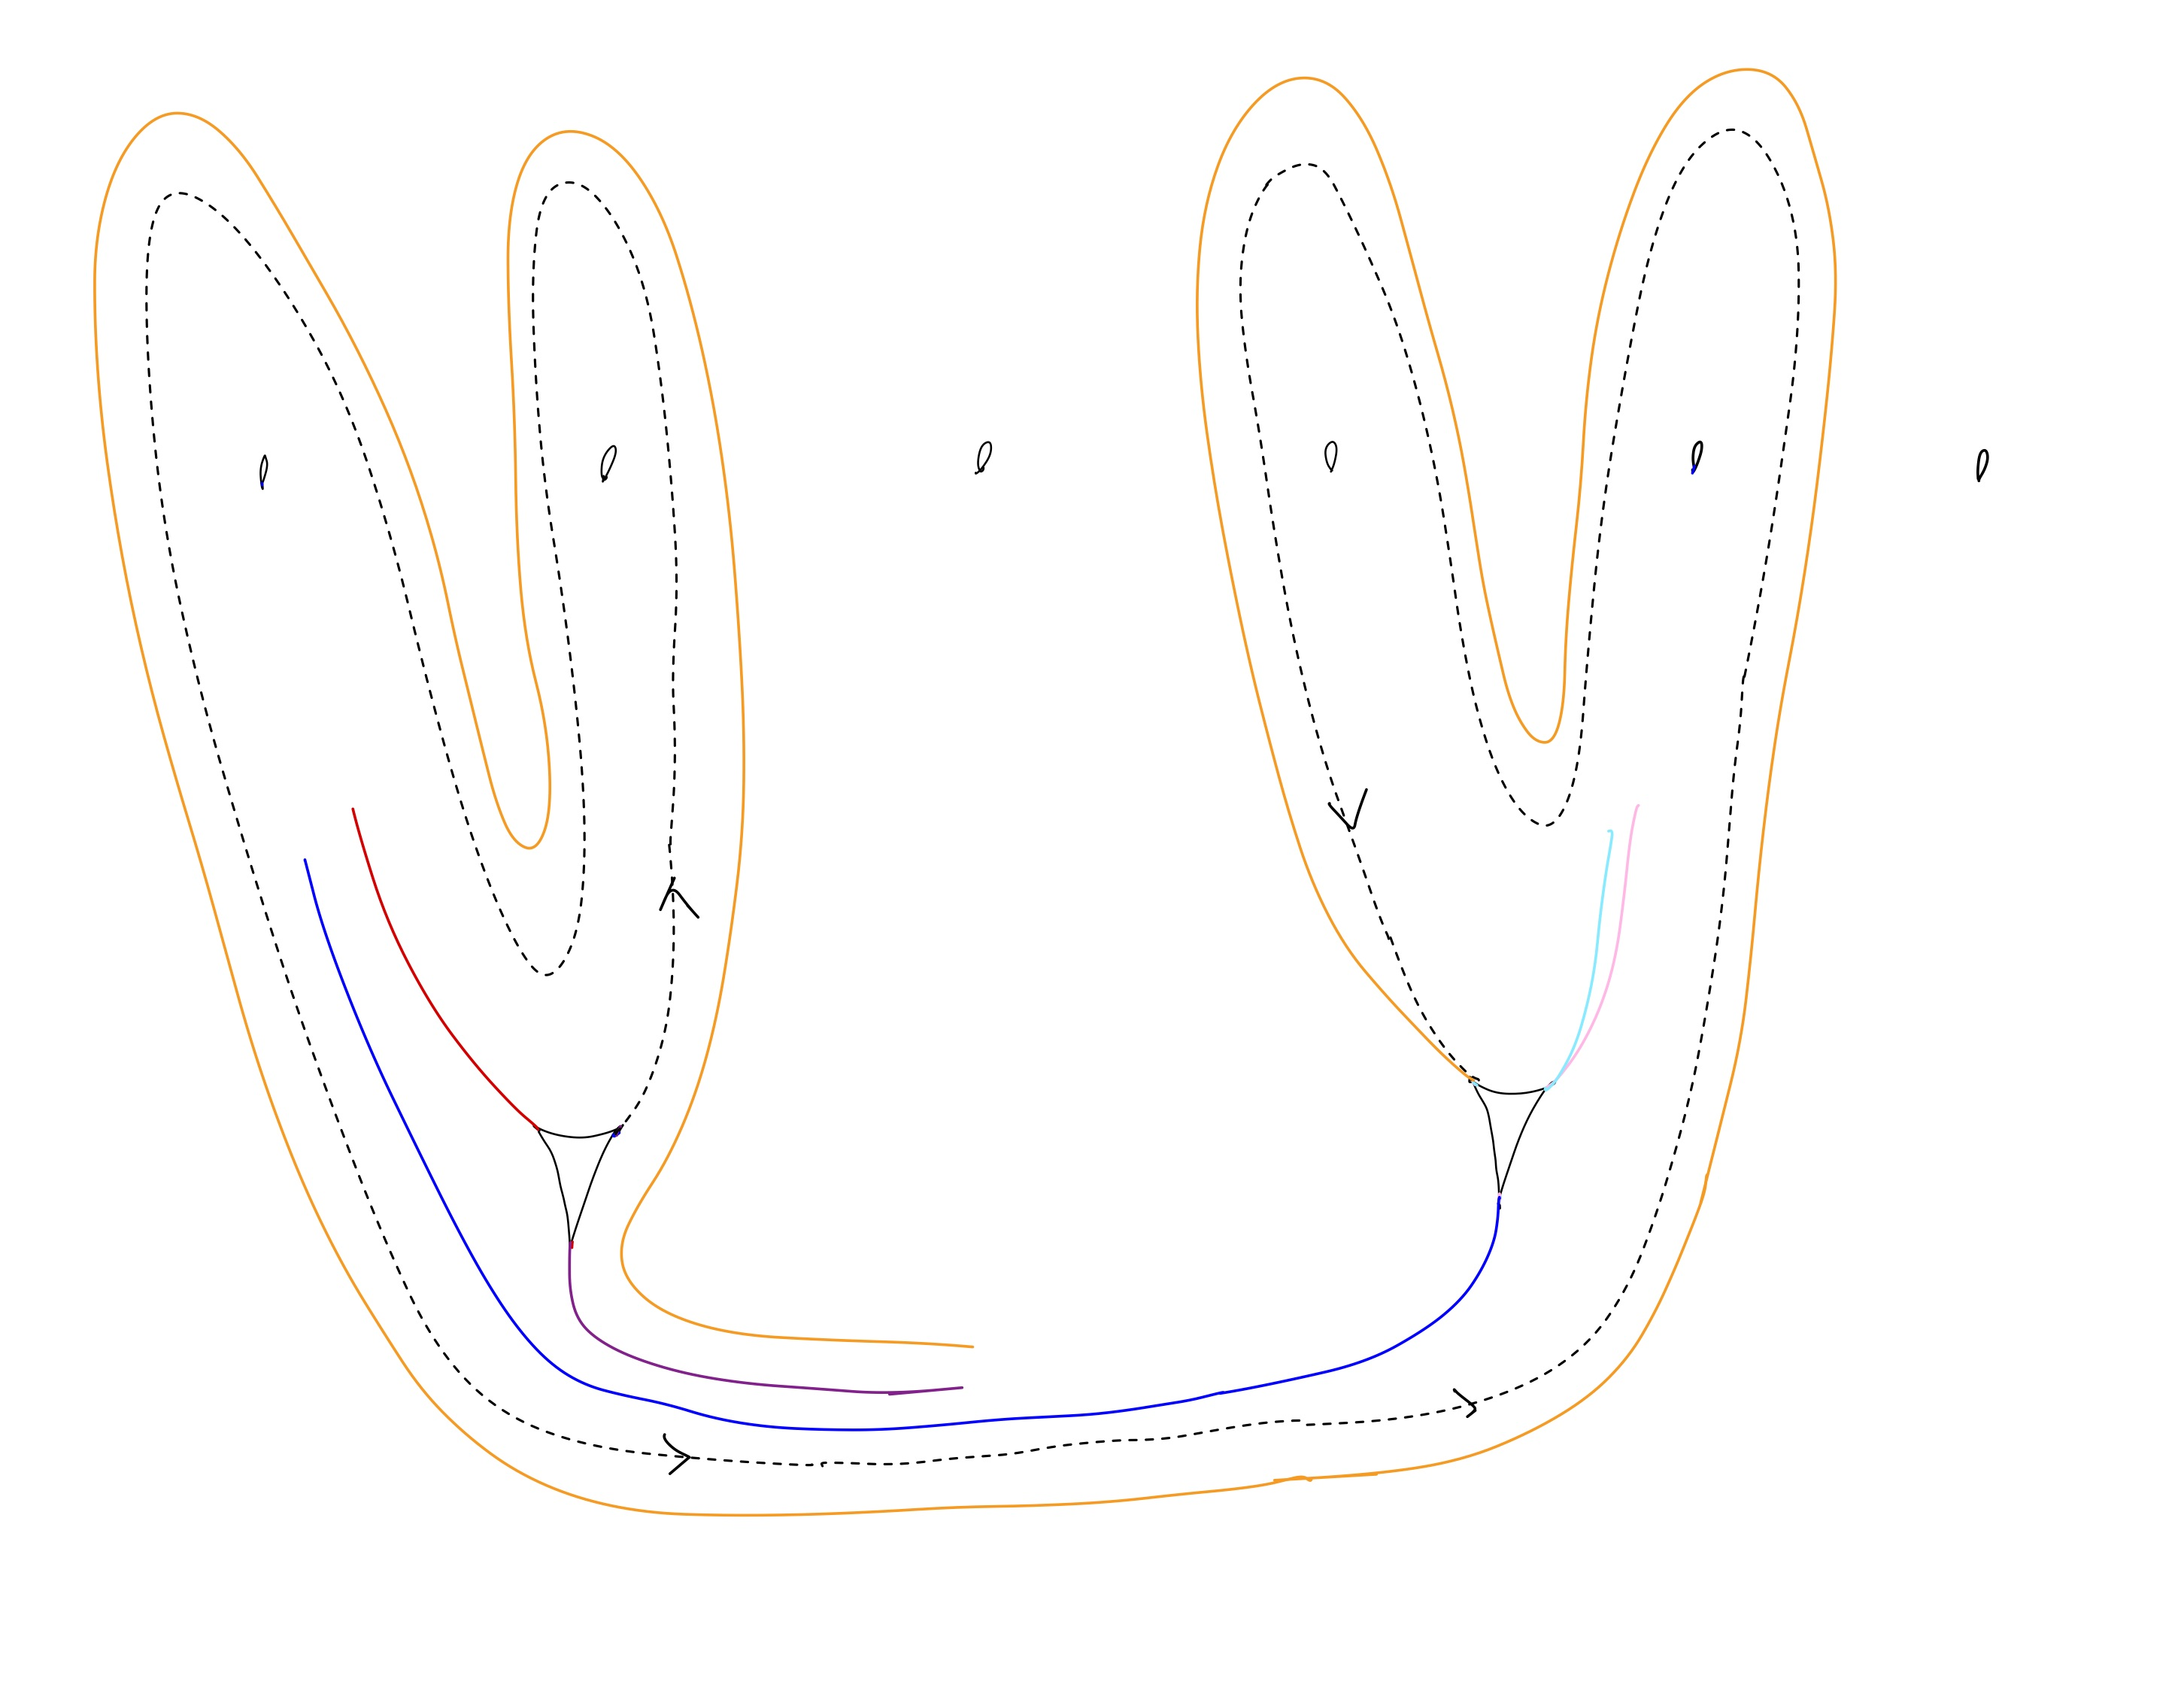
\includegraphics[width=\linewidth]{figures_case_analysis/track17_case_analysis/UAH-5.jpg}
    \caption{UAH5}
    \label{fig:UAH5}
\end{figure}

\begin{figure}[ht]
    \centering
    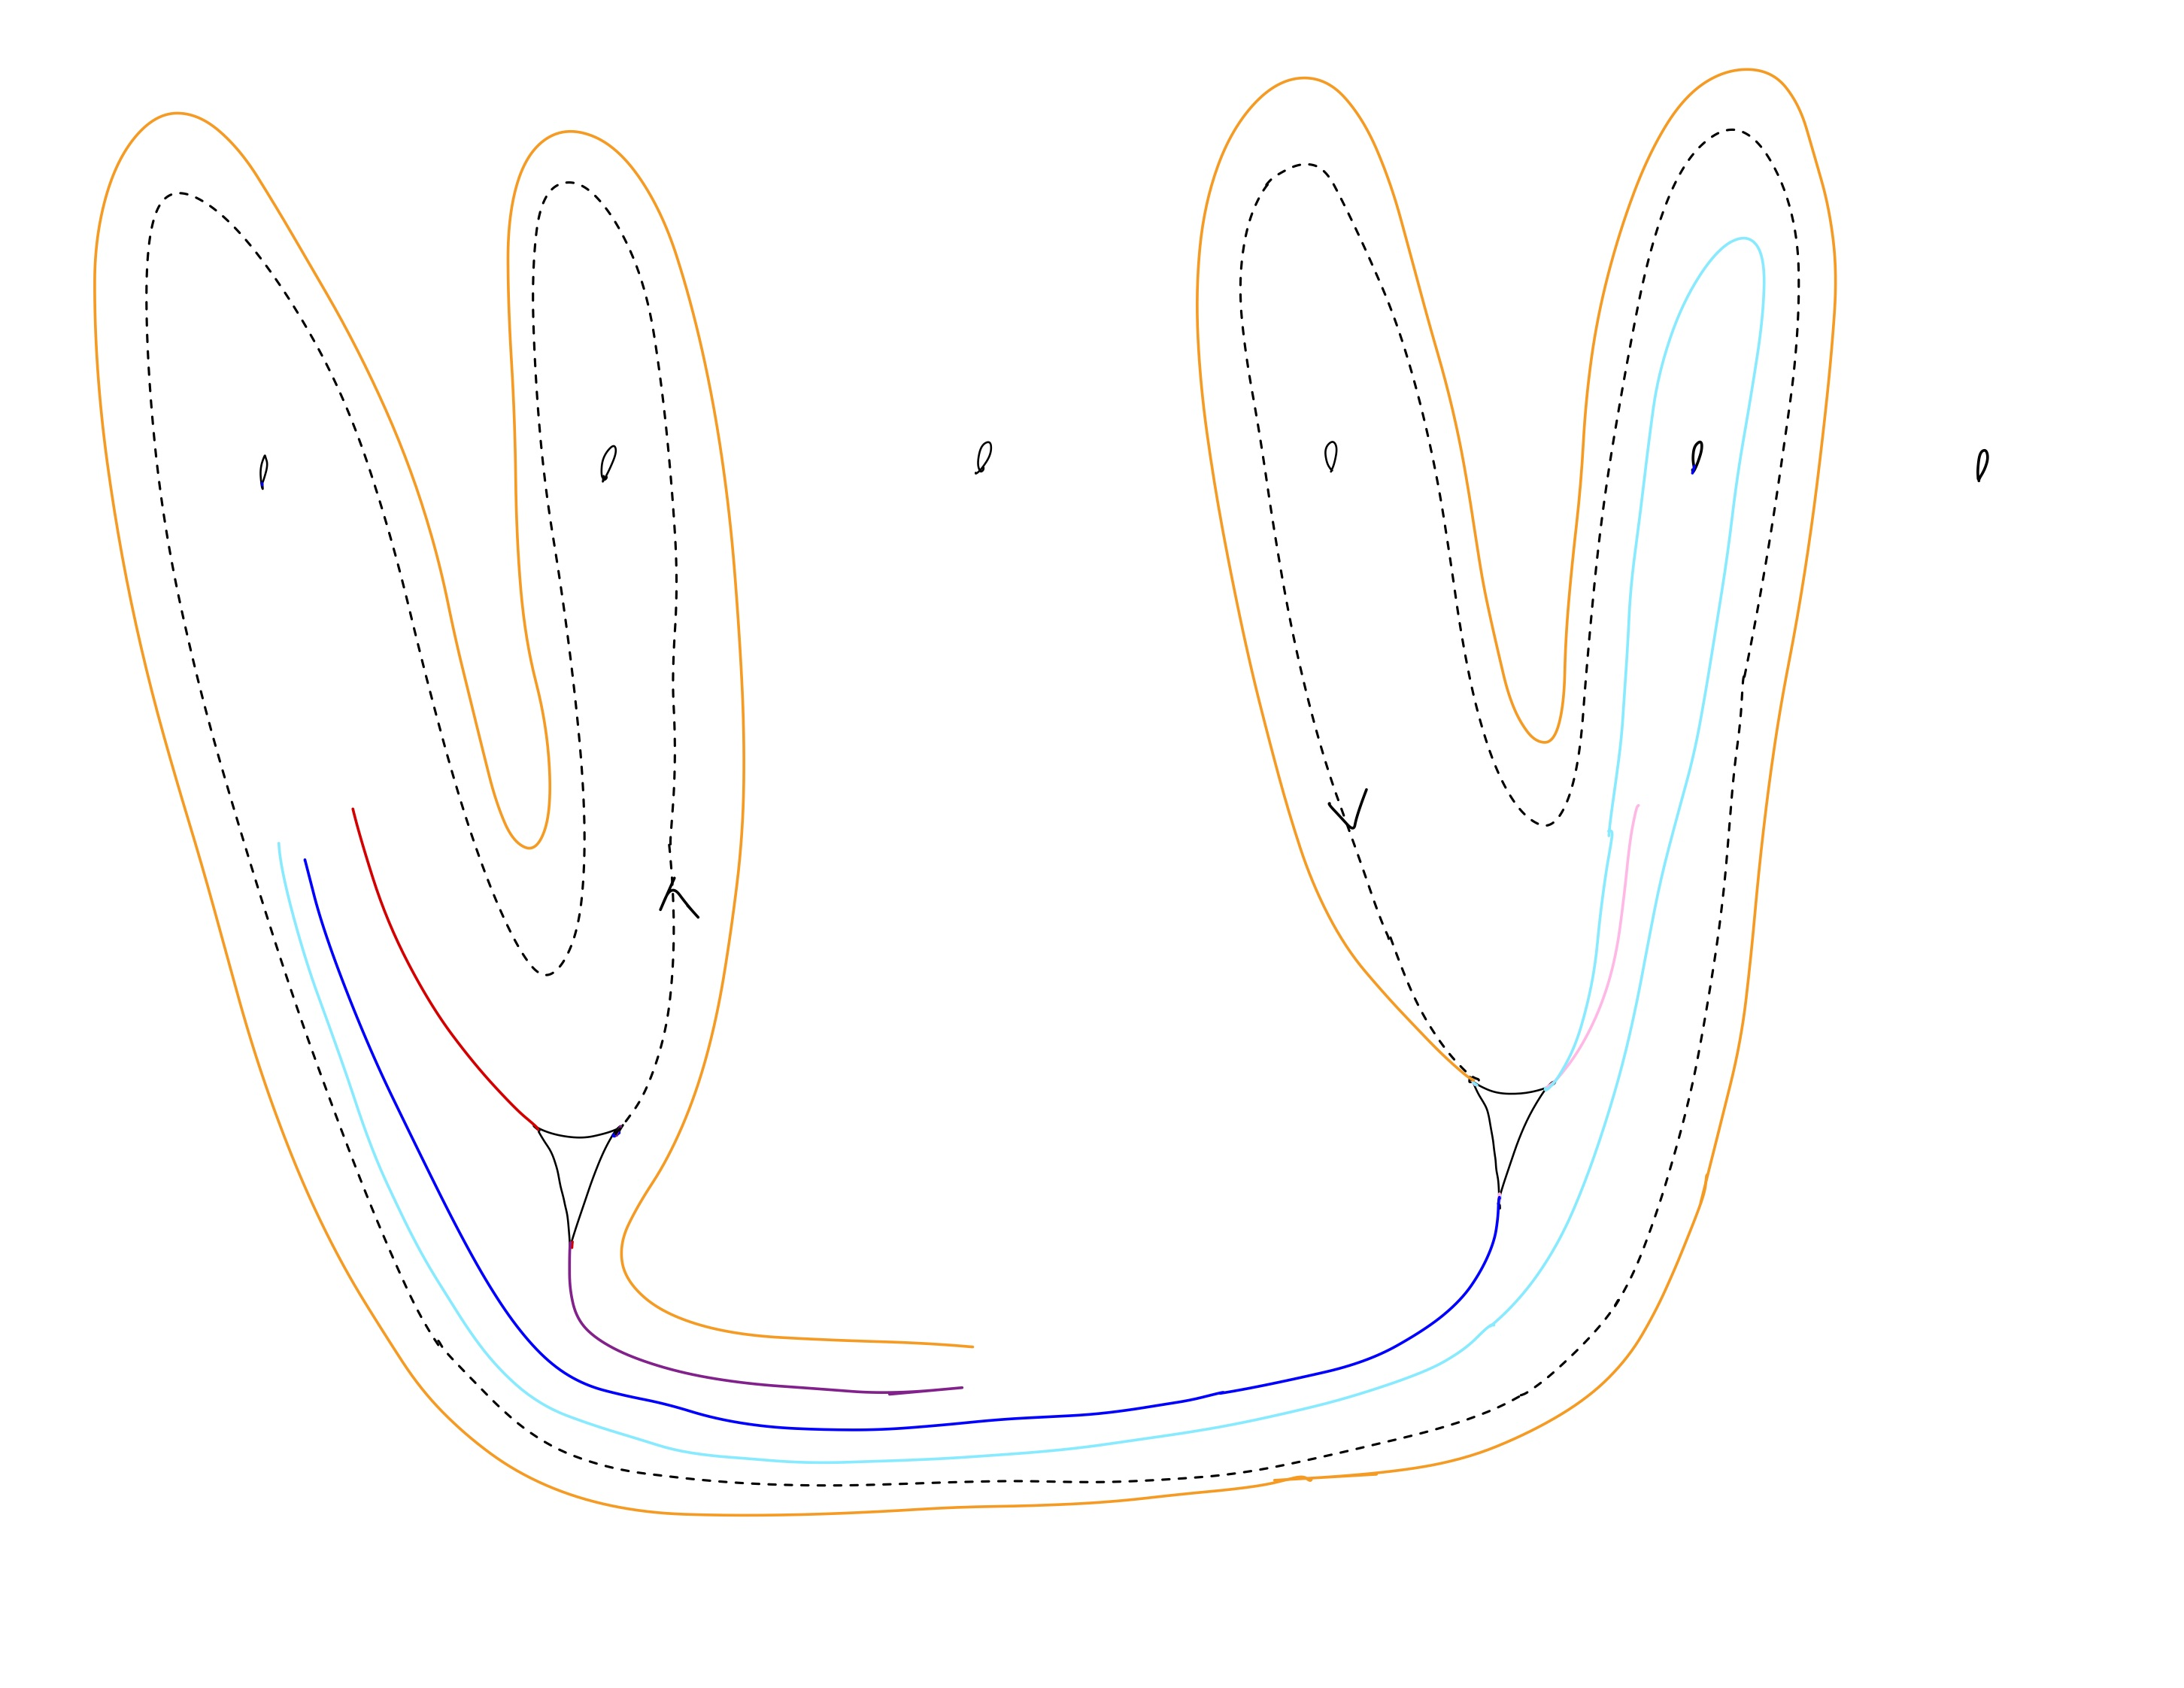
\includegraphics[width=\linewidth]{figures_case_analysis/track17_case_analysis/UAH-6.jpg}
    \caption{UAH6}
    \label{fig:UAH6}
\end{figure}

\begin{figure}[ht]
    \centering
    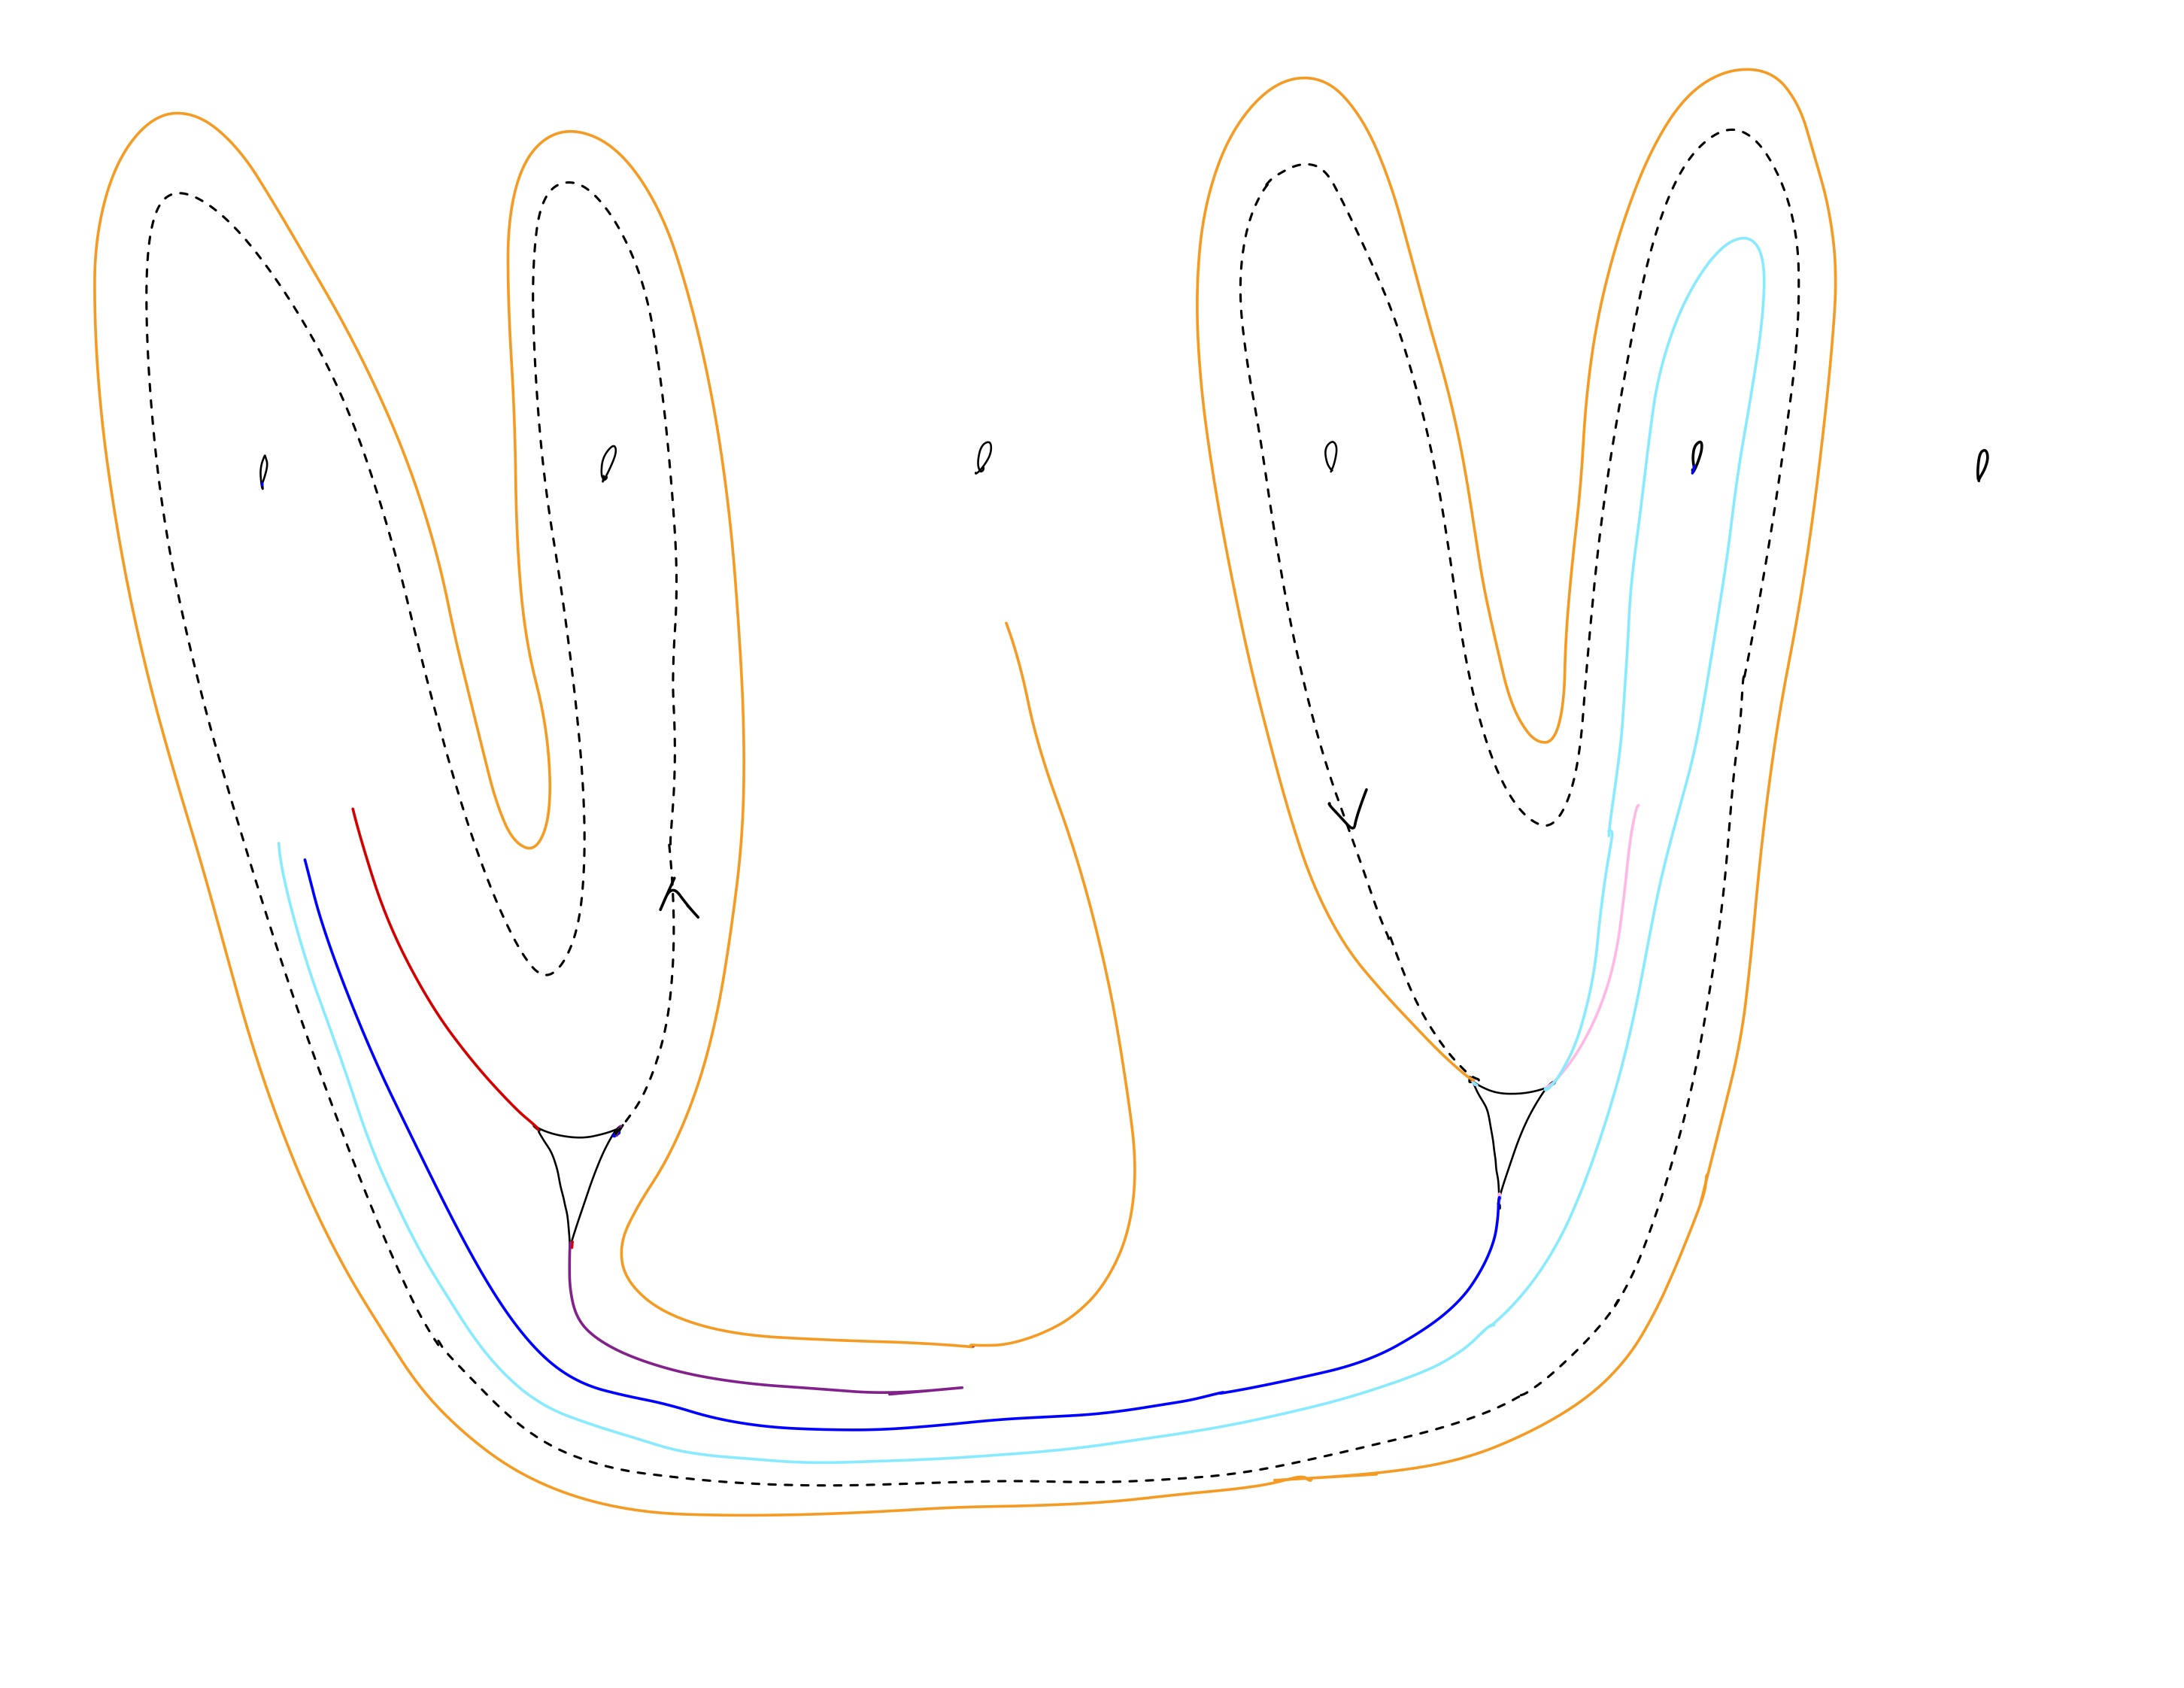
\includegraphics[width=\linewidth]{figures_case_analysis/track17_case_analysis/UAH-7.jpg}
    \caption{UAH7}
    \label{fig:UAH7}
\end{figure}
\clearpage

\begin{figure}[ht]
    \centering
    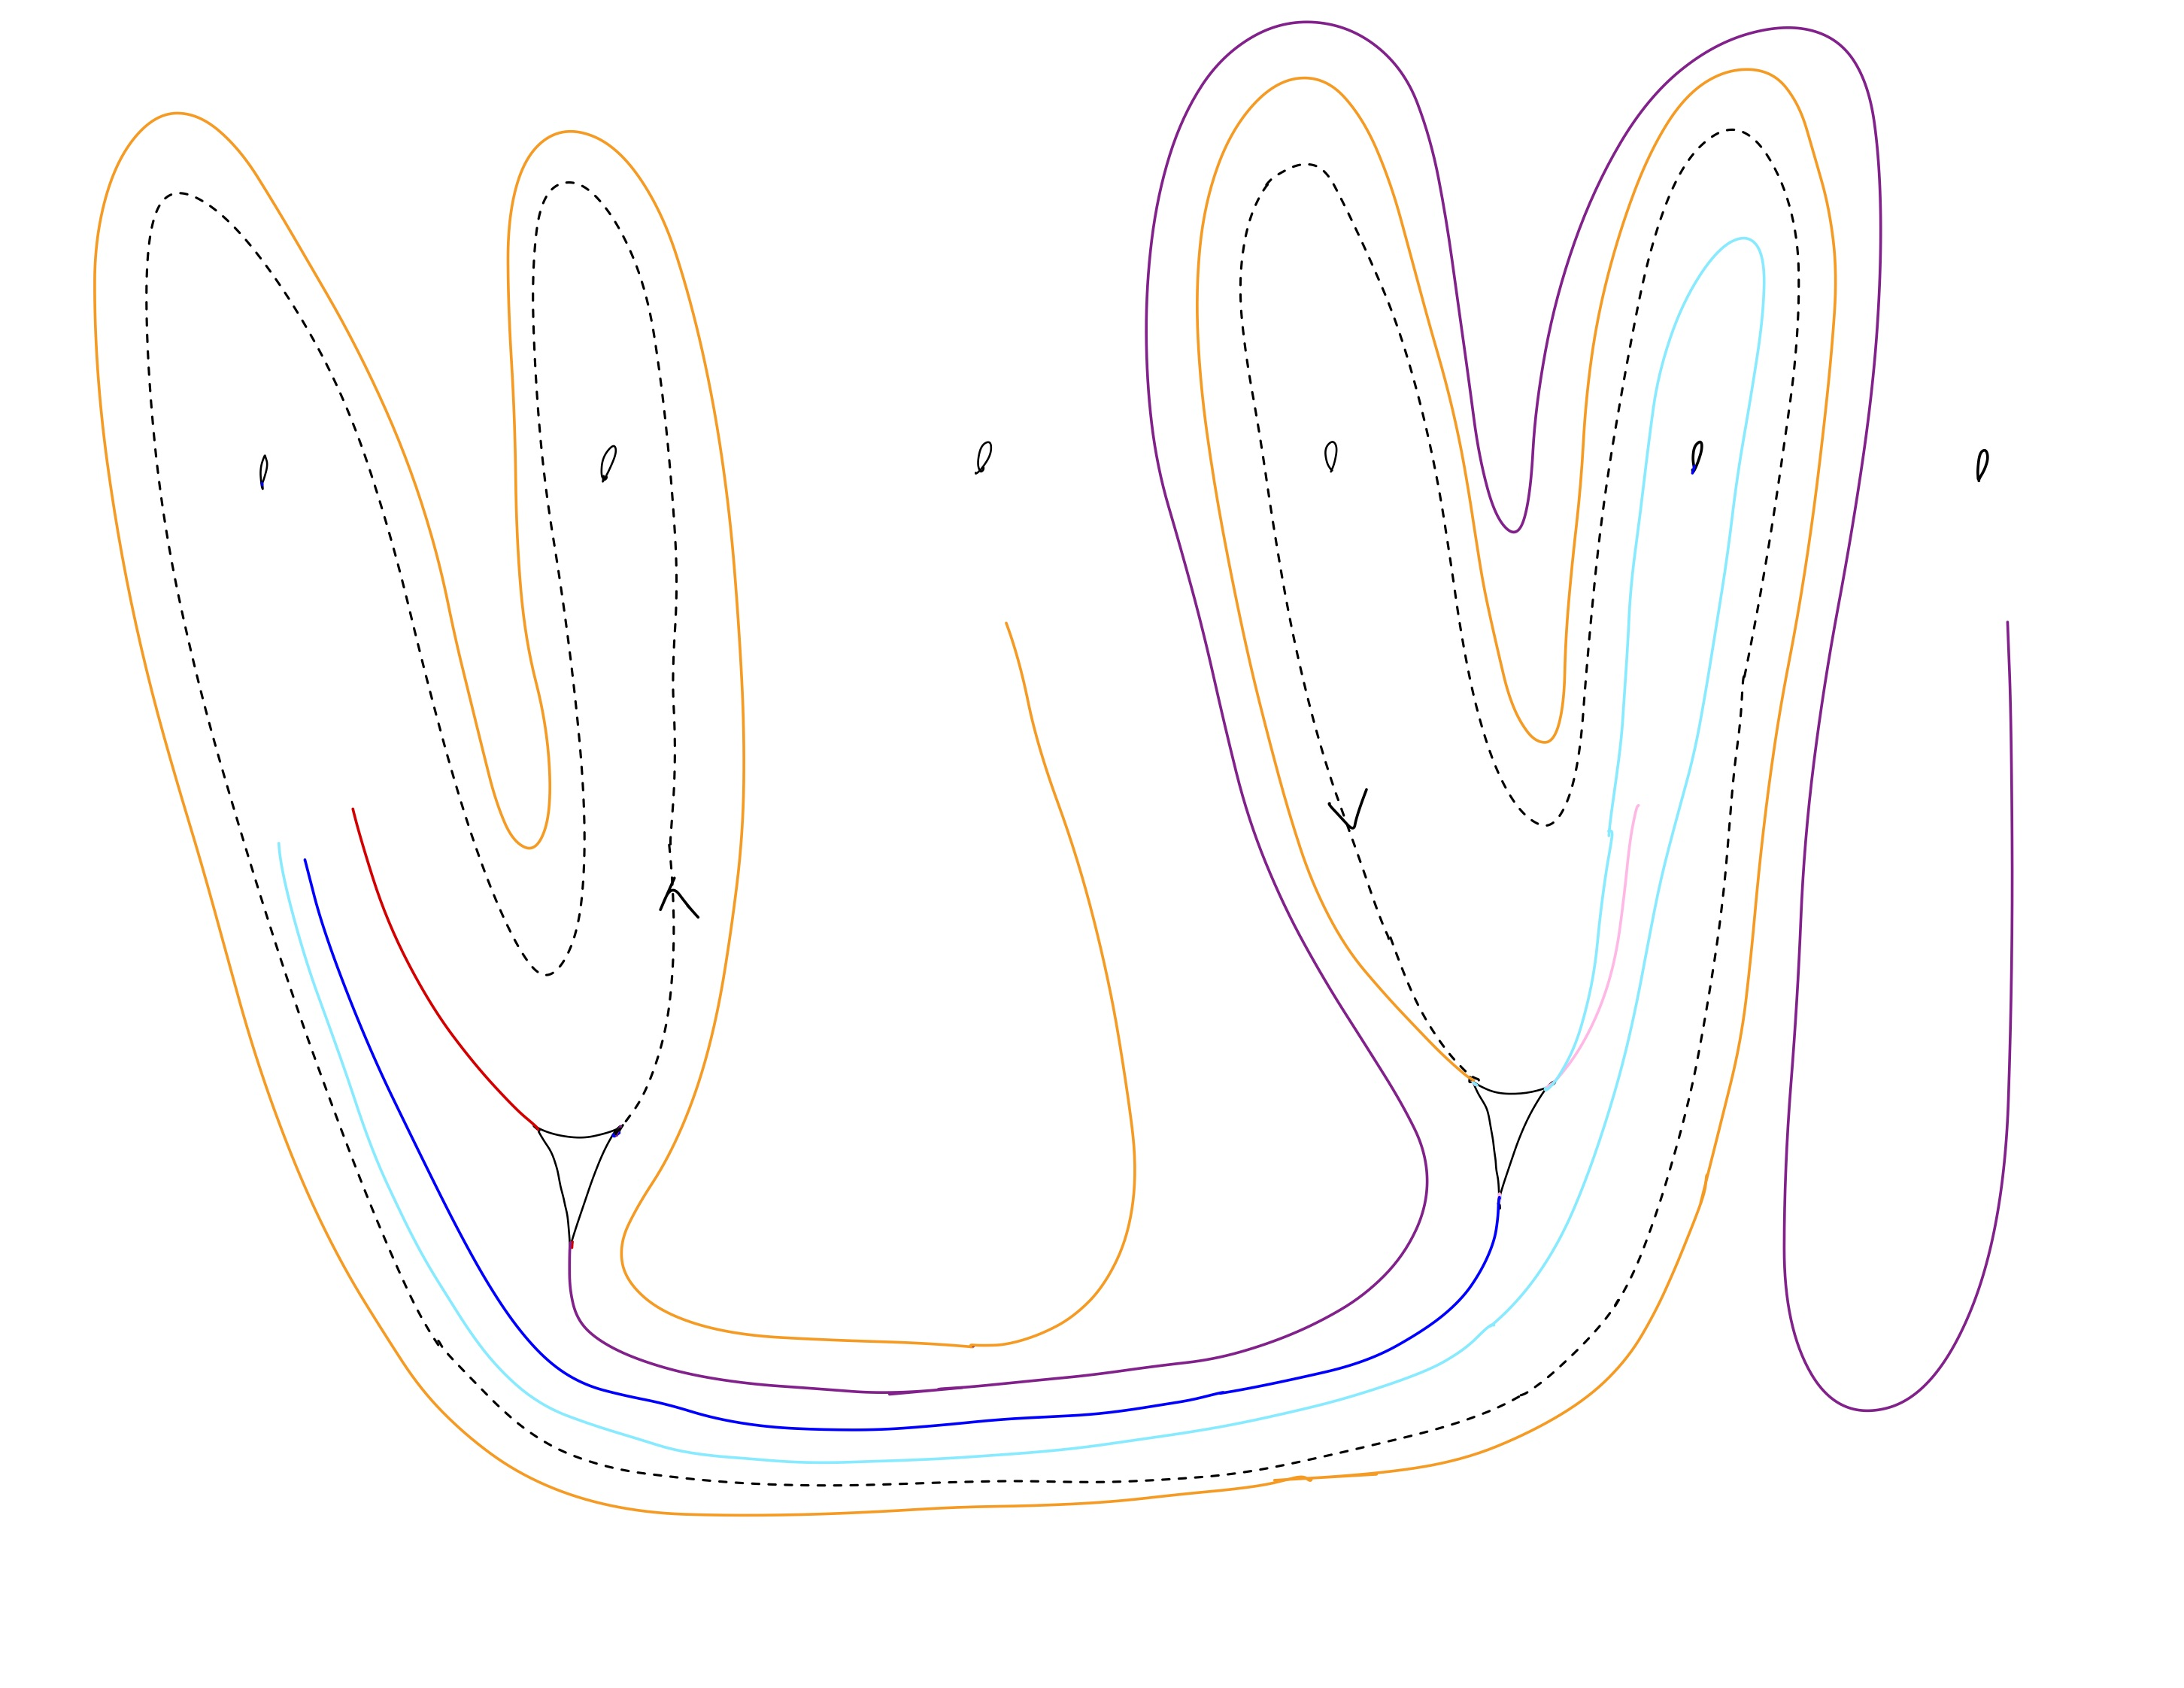
\includegraphics[width=\linewidth]{figures_case_analysis/track17_case_analysis/Oche-1.jpg}
    \caption{Oche1}
    \label{fig:Oche1}
\end{figure}

\begin{figure}[ht]
    \centering
    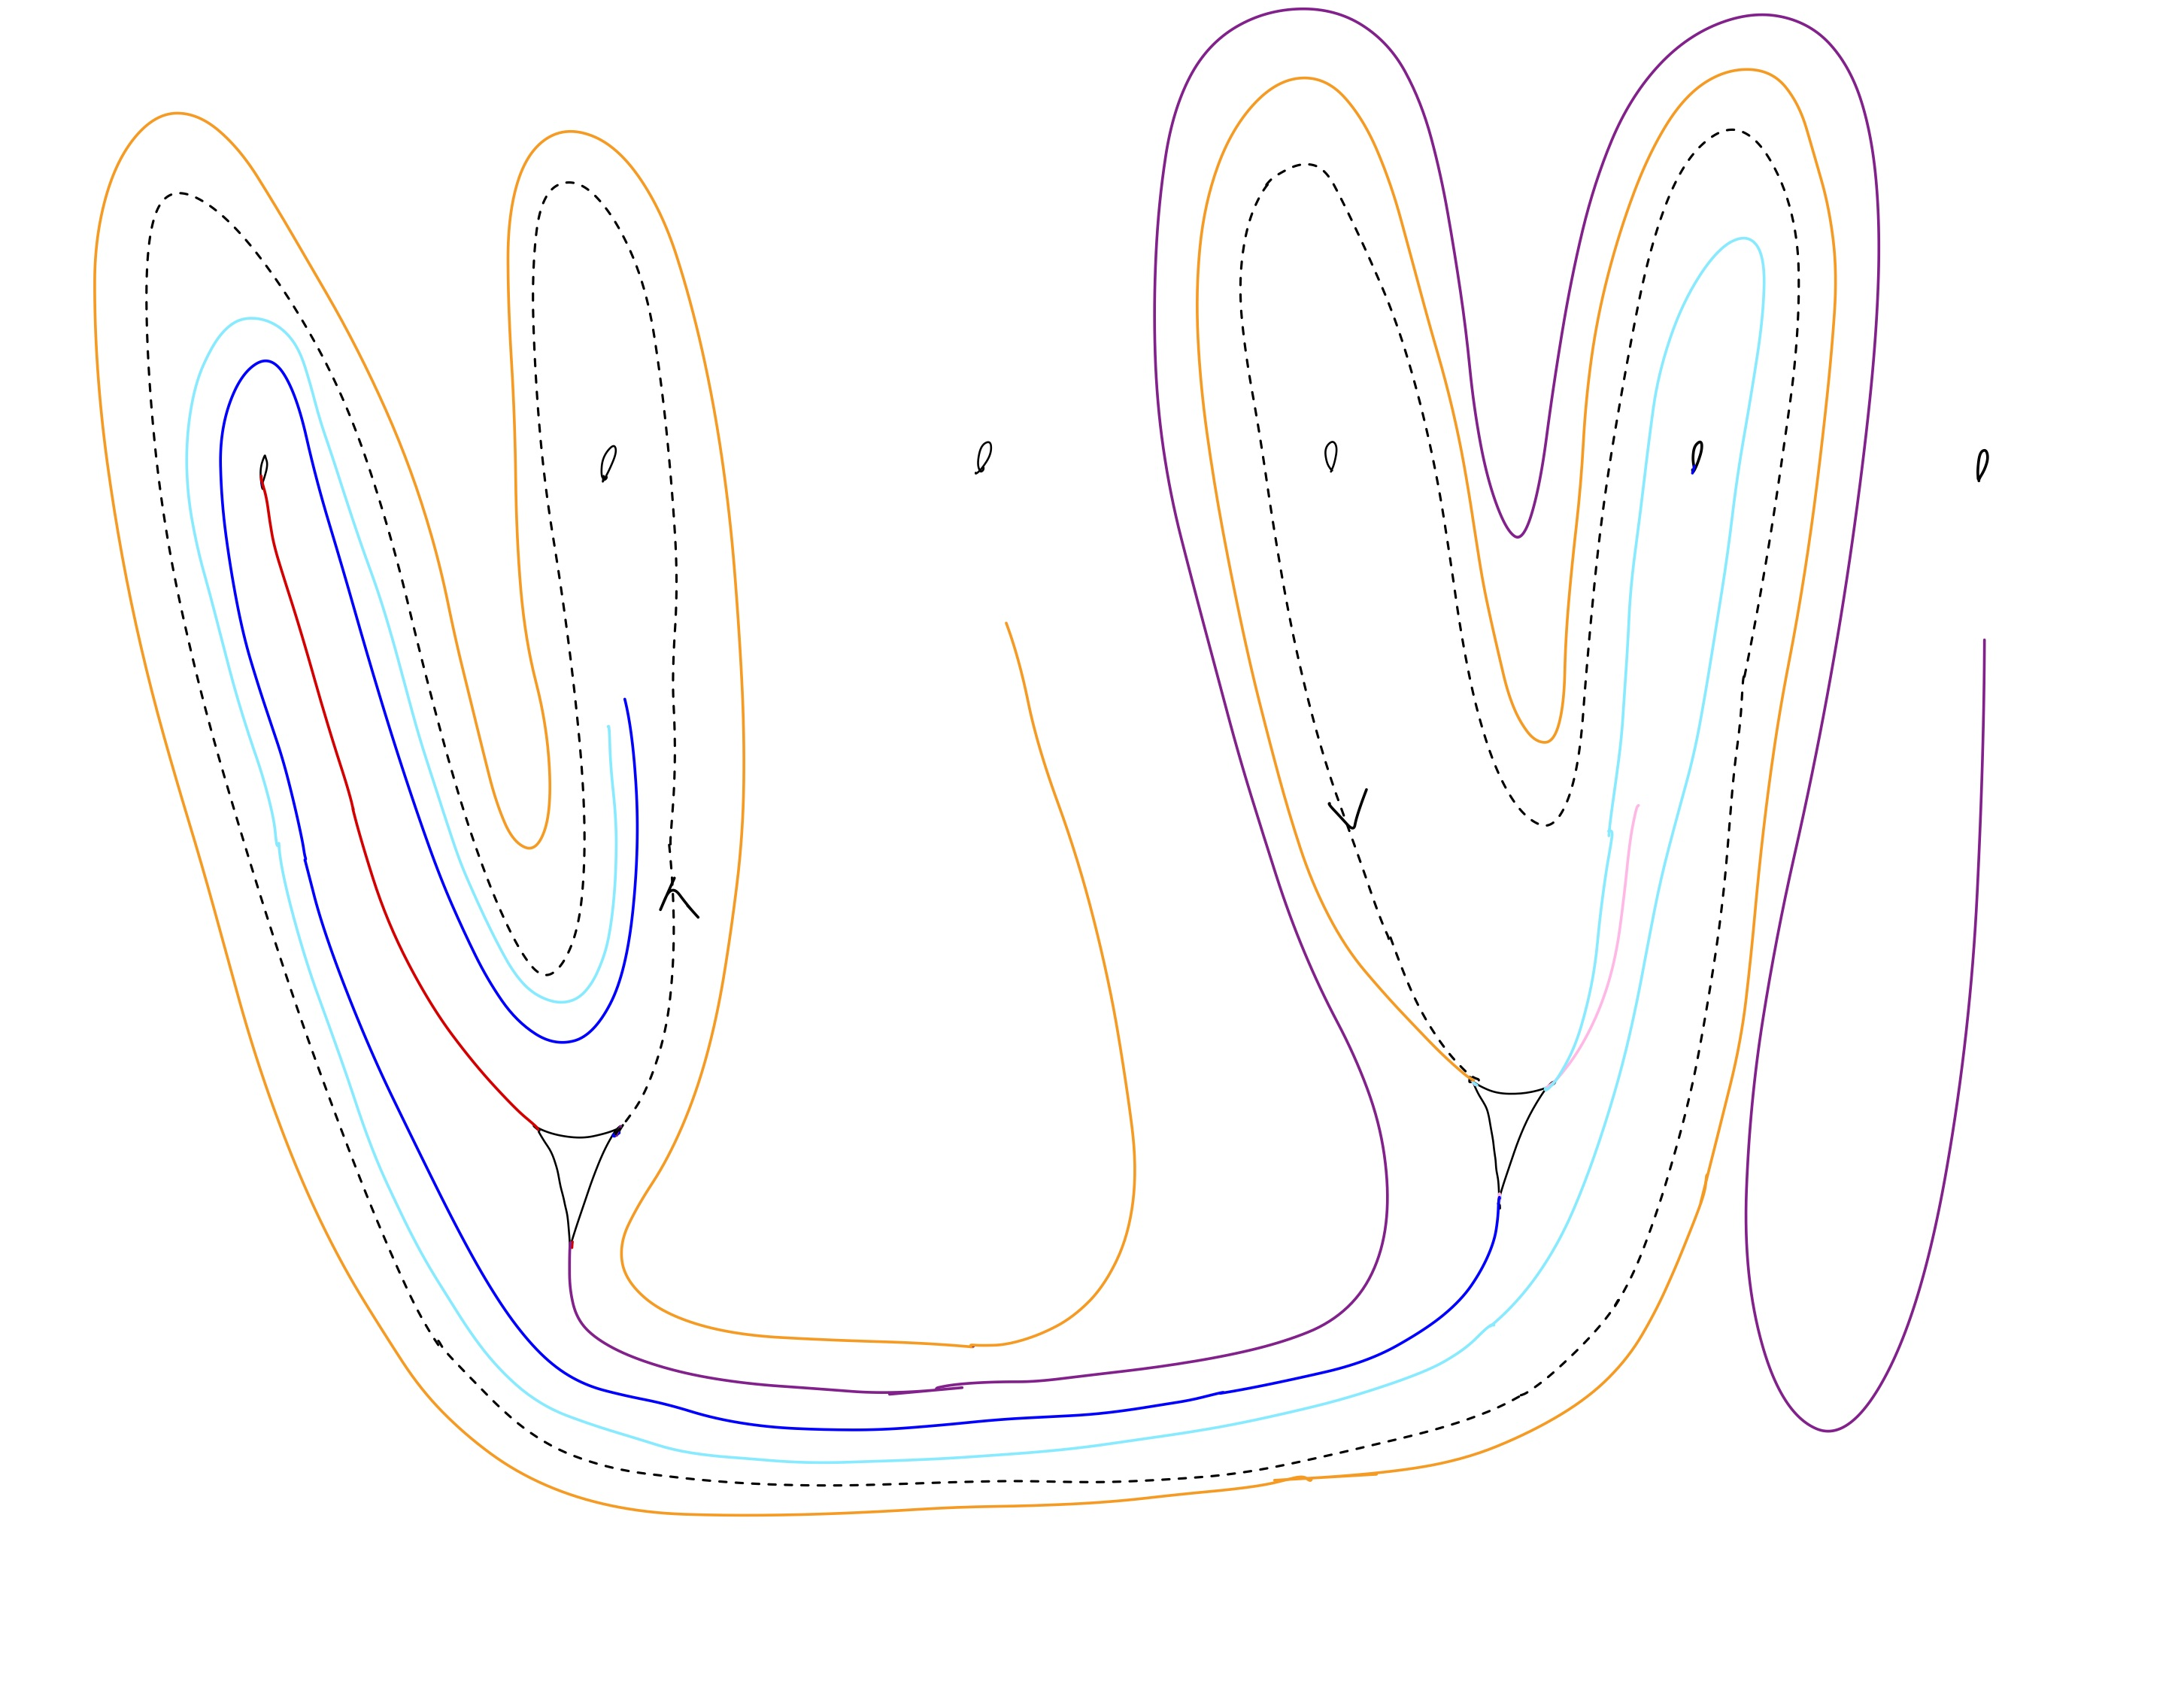
\includegraphics[width=\linewidth]{figures_case_analysis/track17_case_analysis/Oche-2.jpg}
    \caption{Oche2}
    \label{fig:Oche2}
\end{figure}

\begin{figure}[ht]
    \centering
    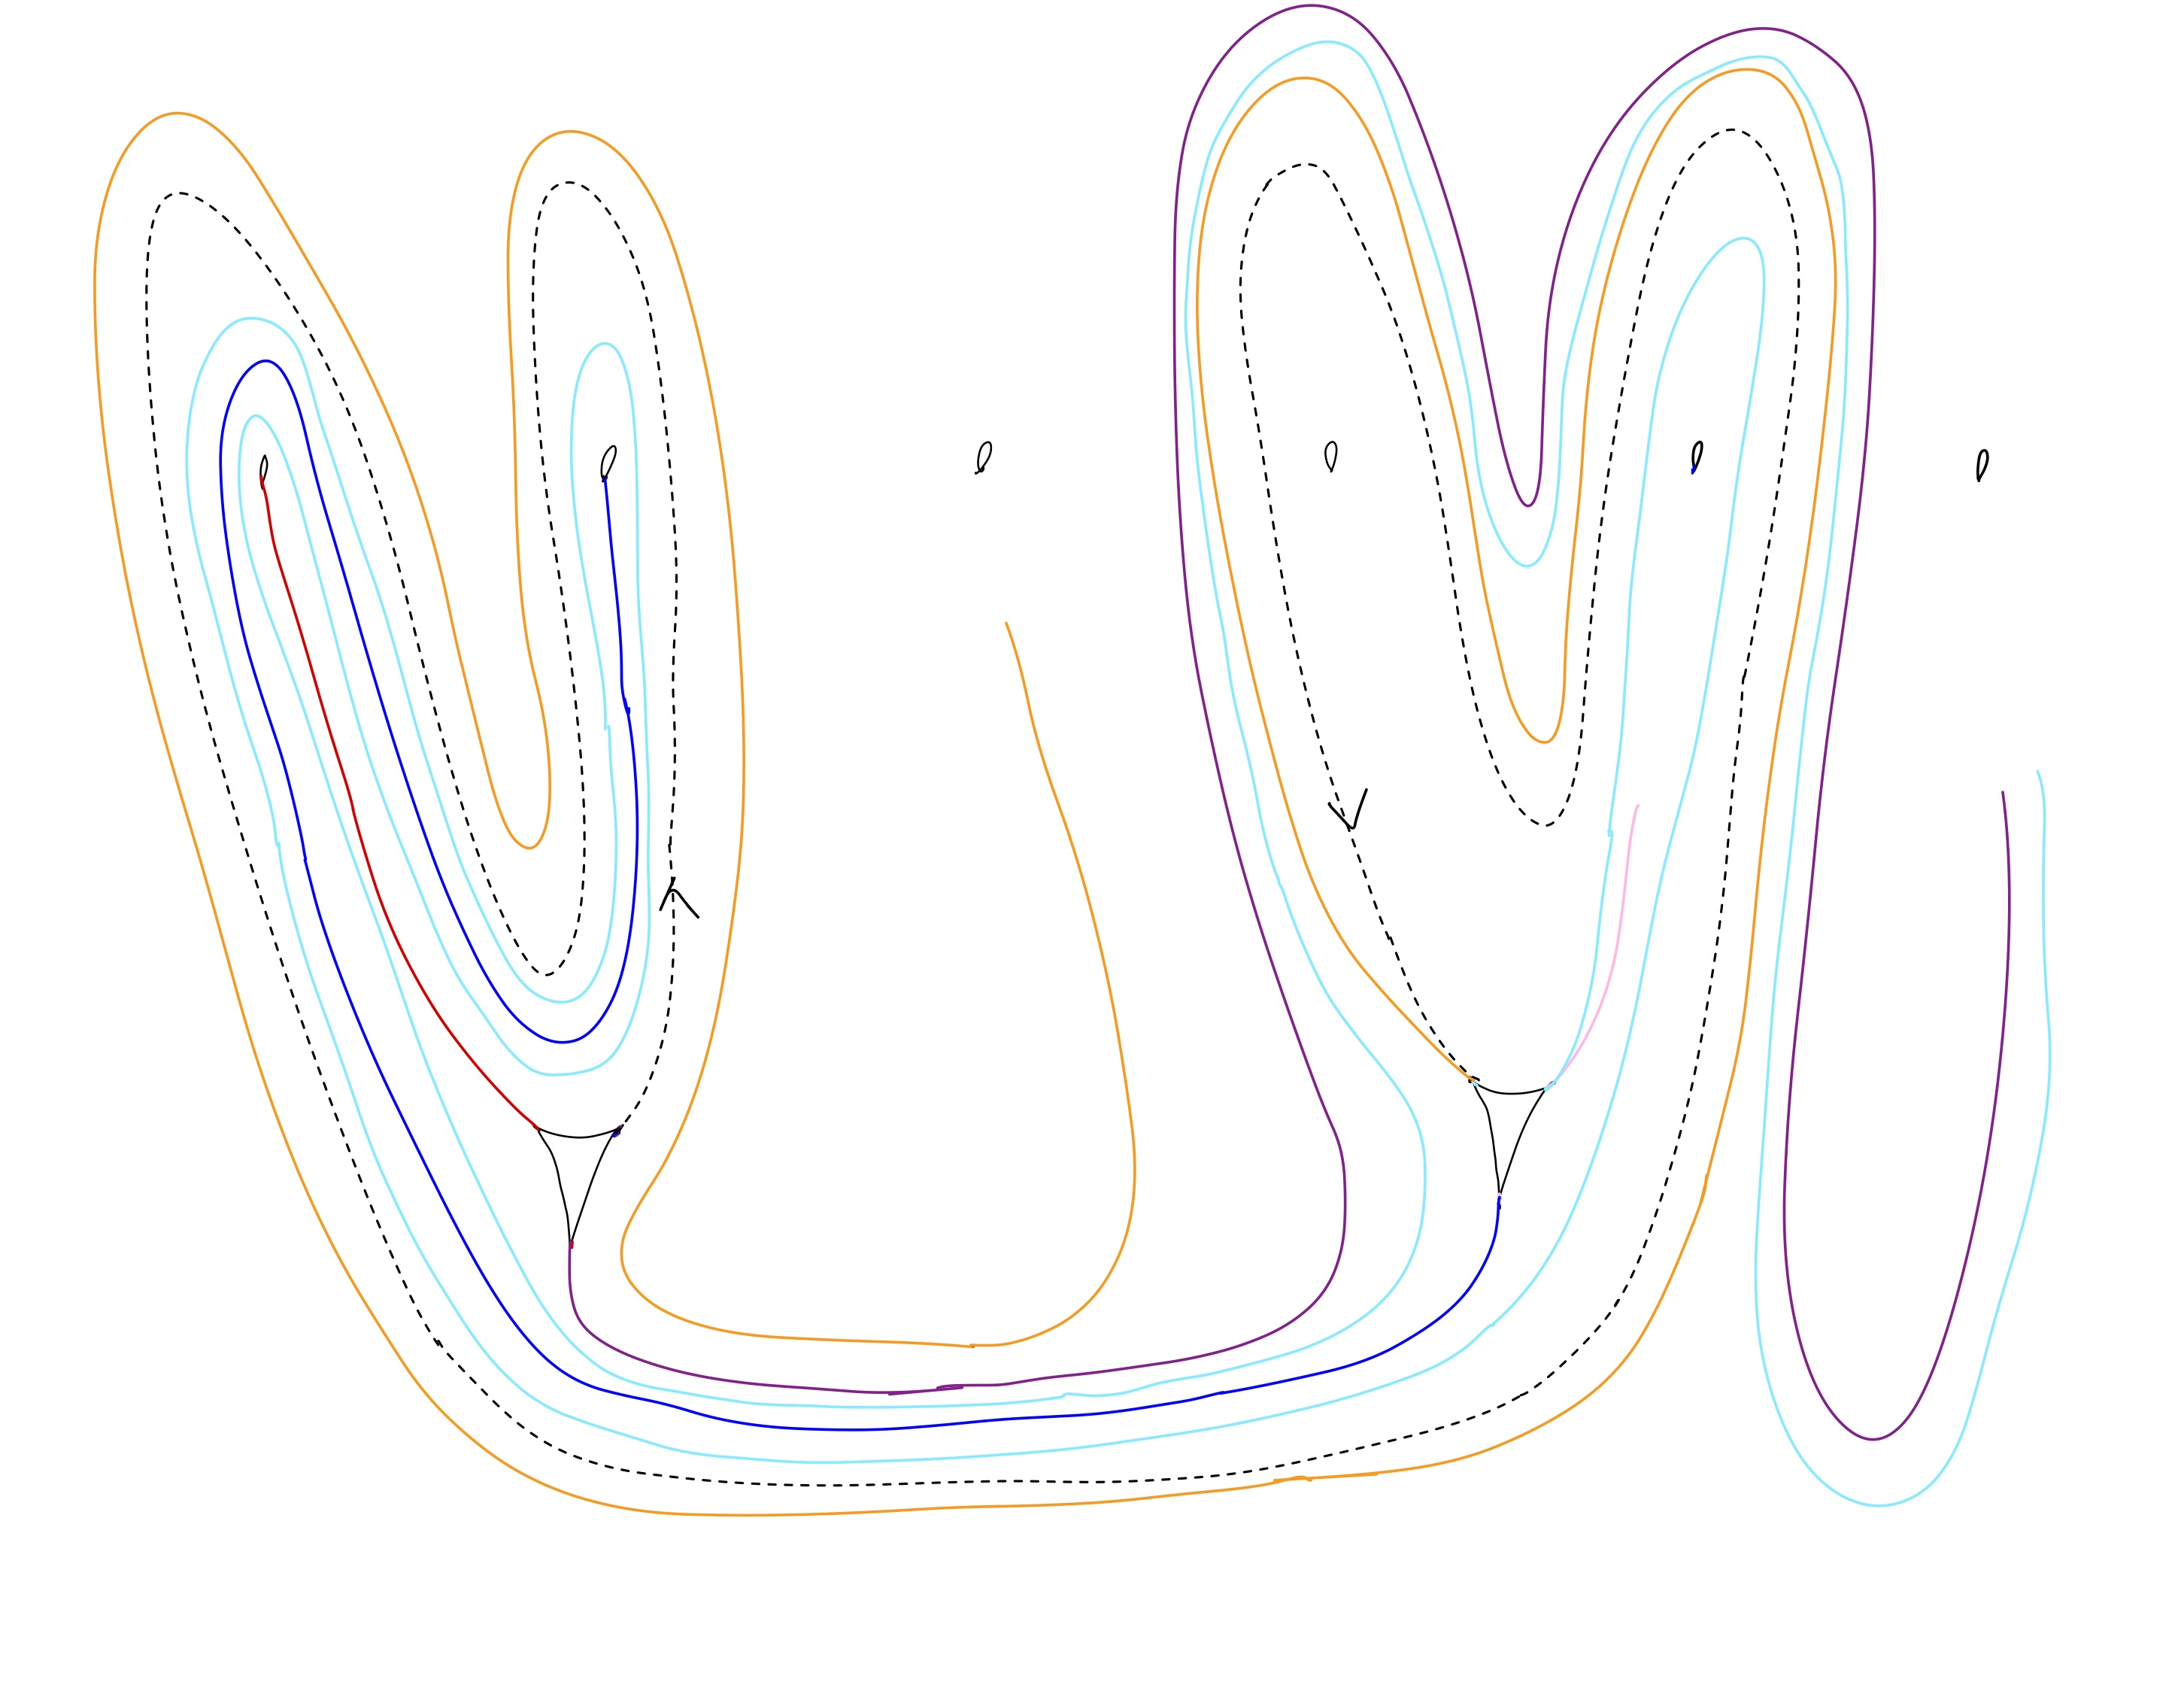
\includegraphics[width=\linewidth]{figures_case_analysis/track17_case_analysis/Oche-3.jpg}
    \caption{Oche3}
    \label{fig:Oche3}
\end{figure}

\begin{figure}[ht]
    \centering
    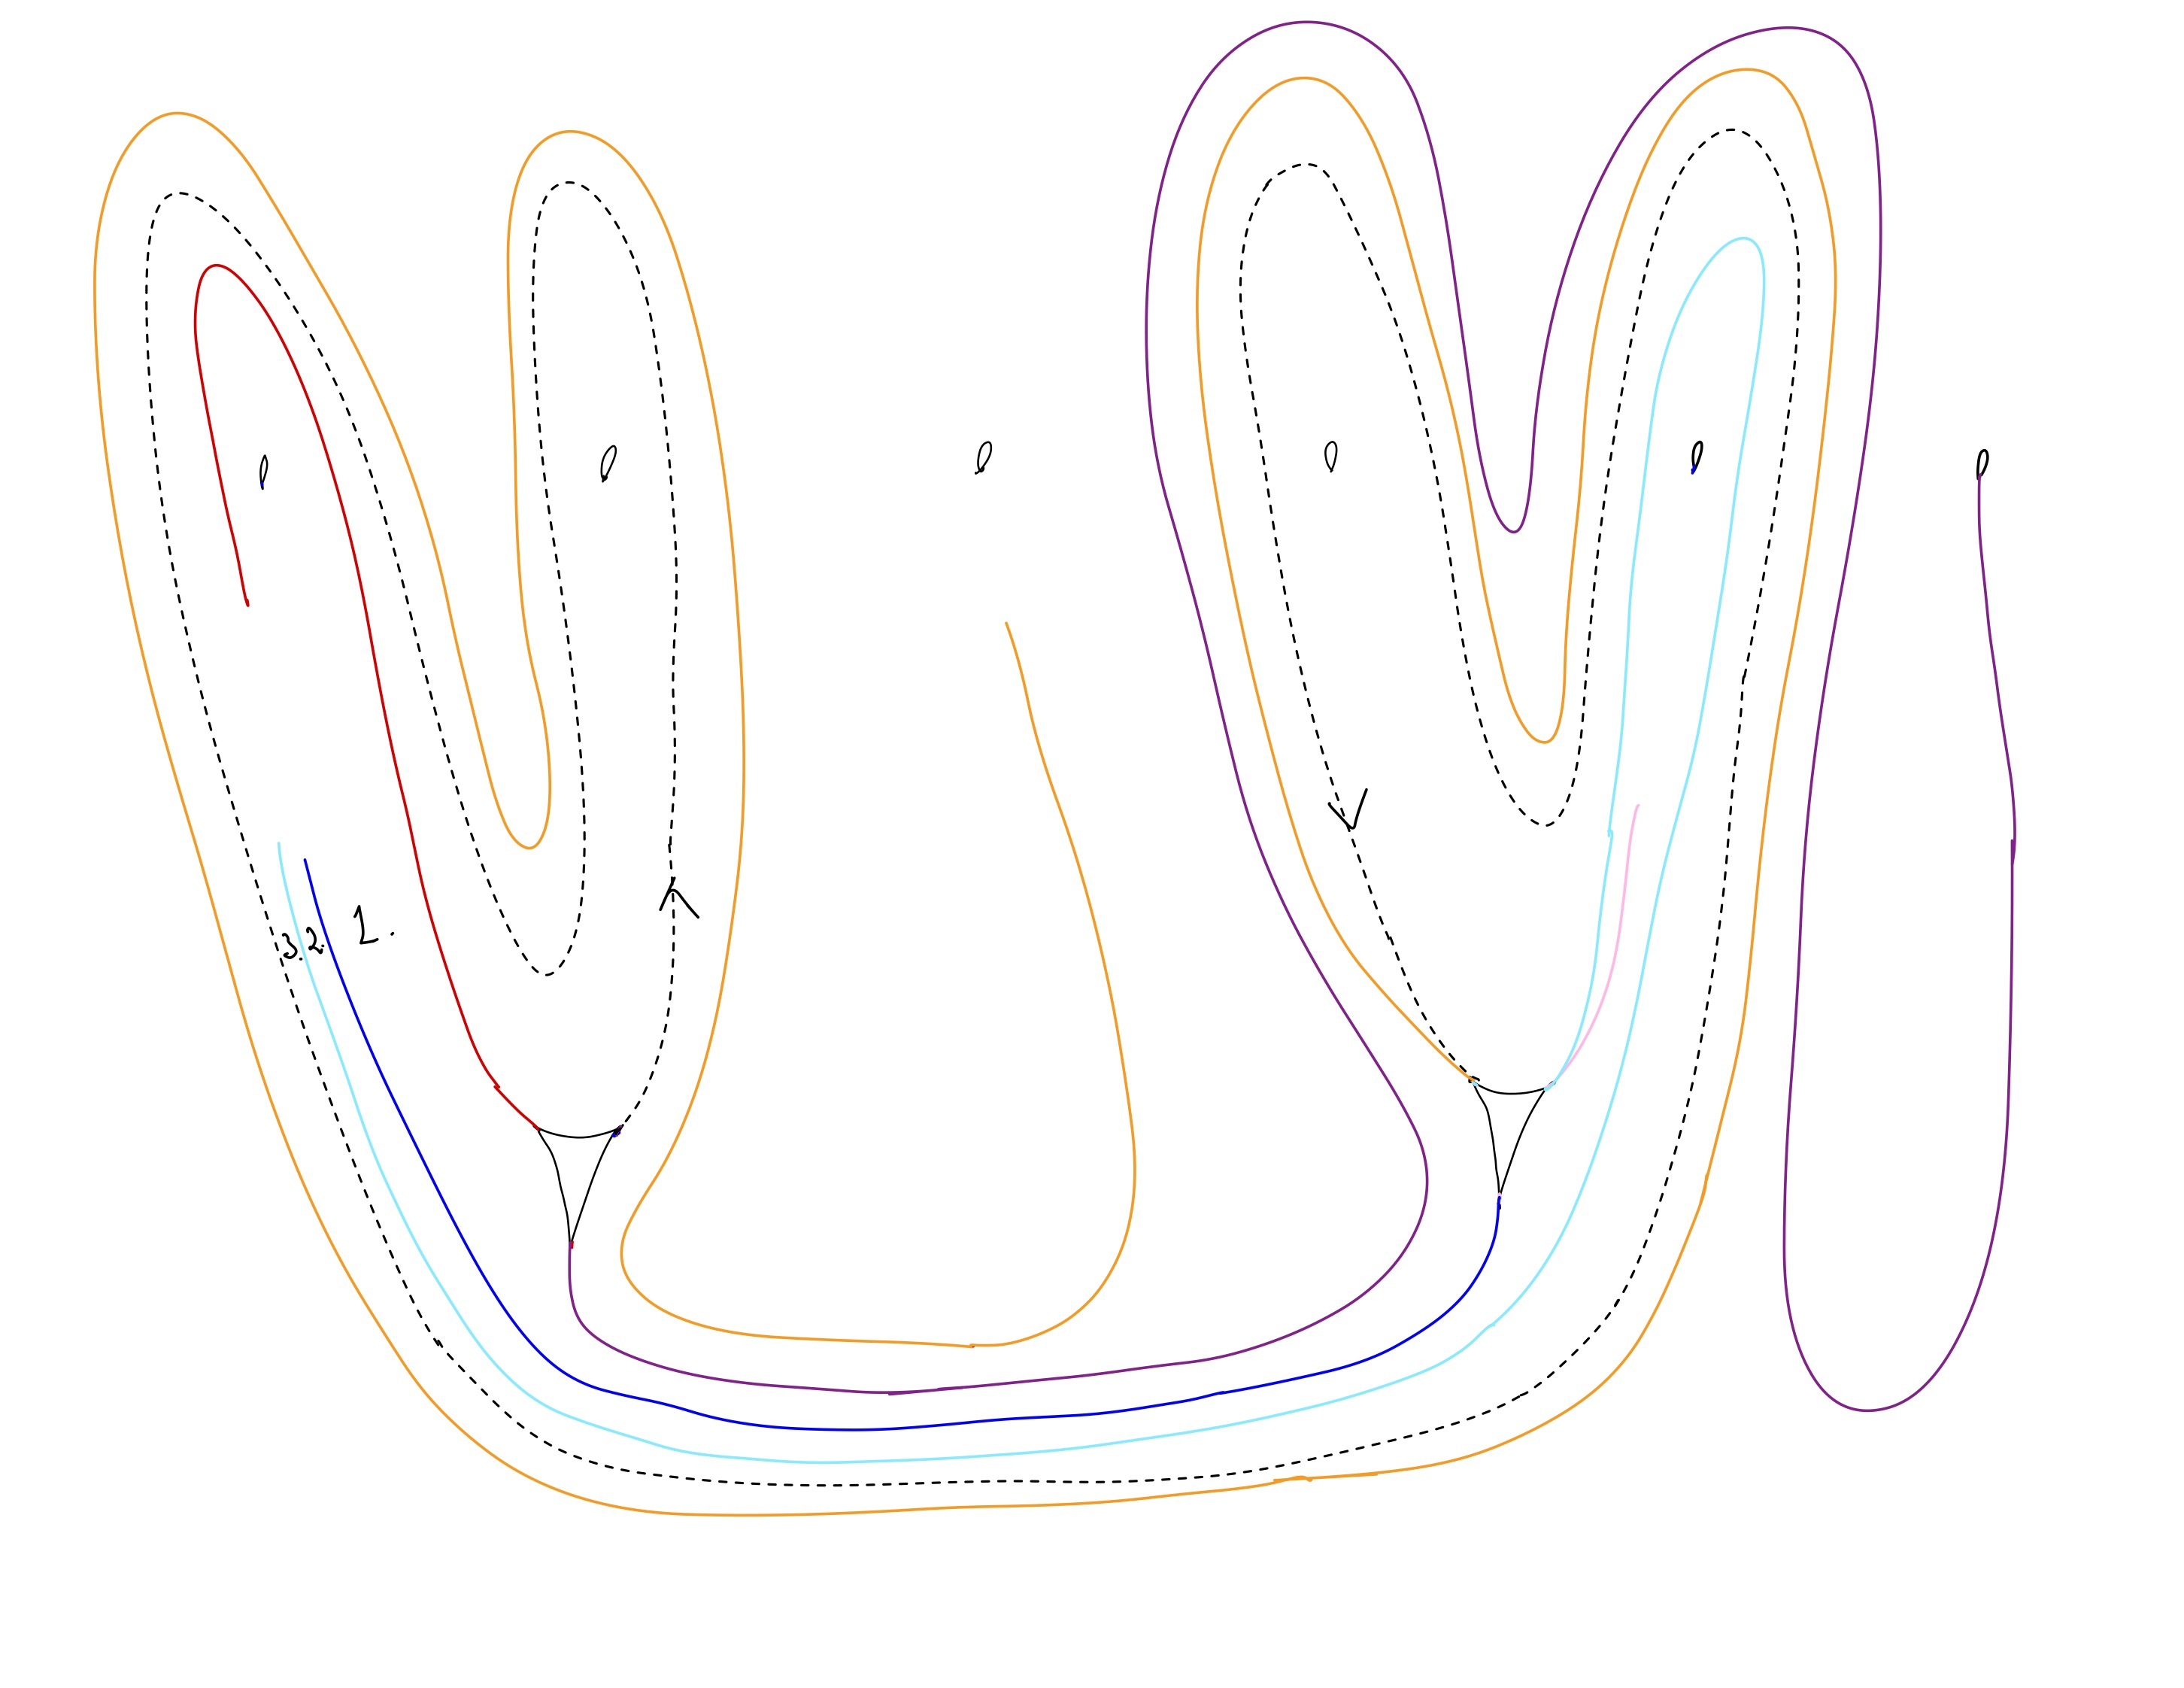
\includegraphics[width=\linewidth]{figures_case_analysis/track17_case_analysis/Oche-4.jpg}
    \caption{Oche4}
    \label{fig:Oche4}
\end{figure}

\begin{figure}[ht]
    \centering
    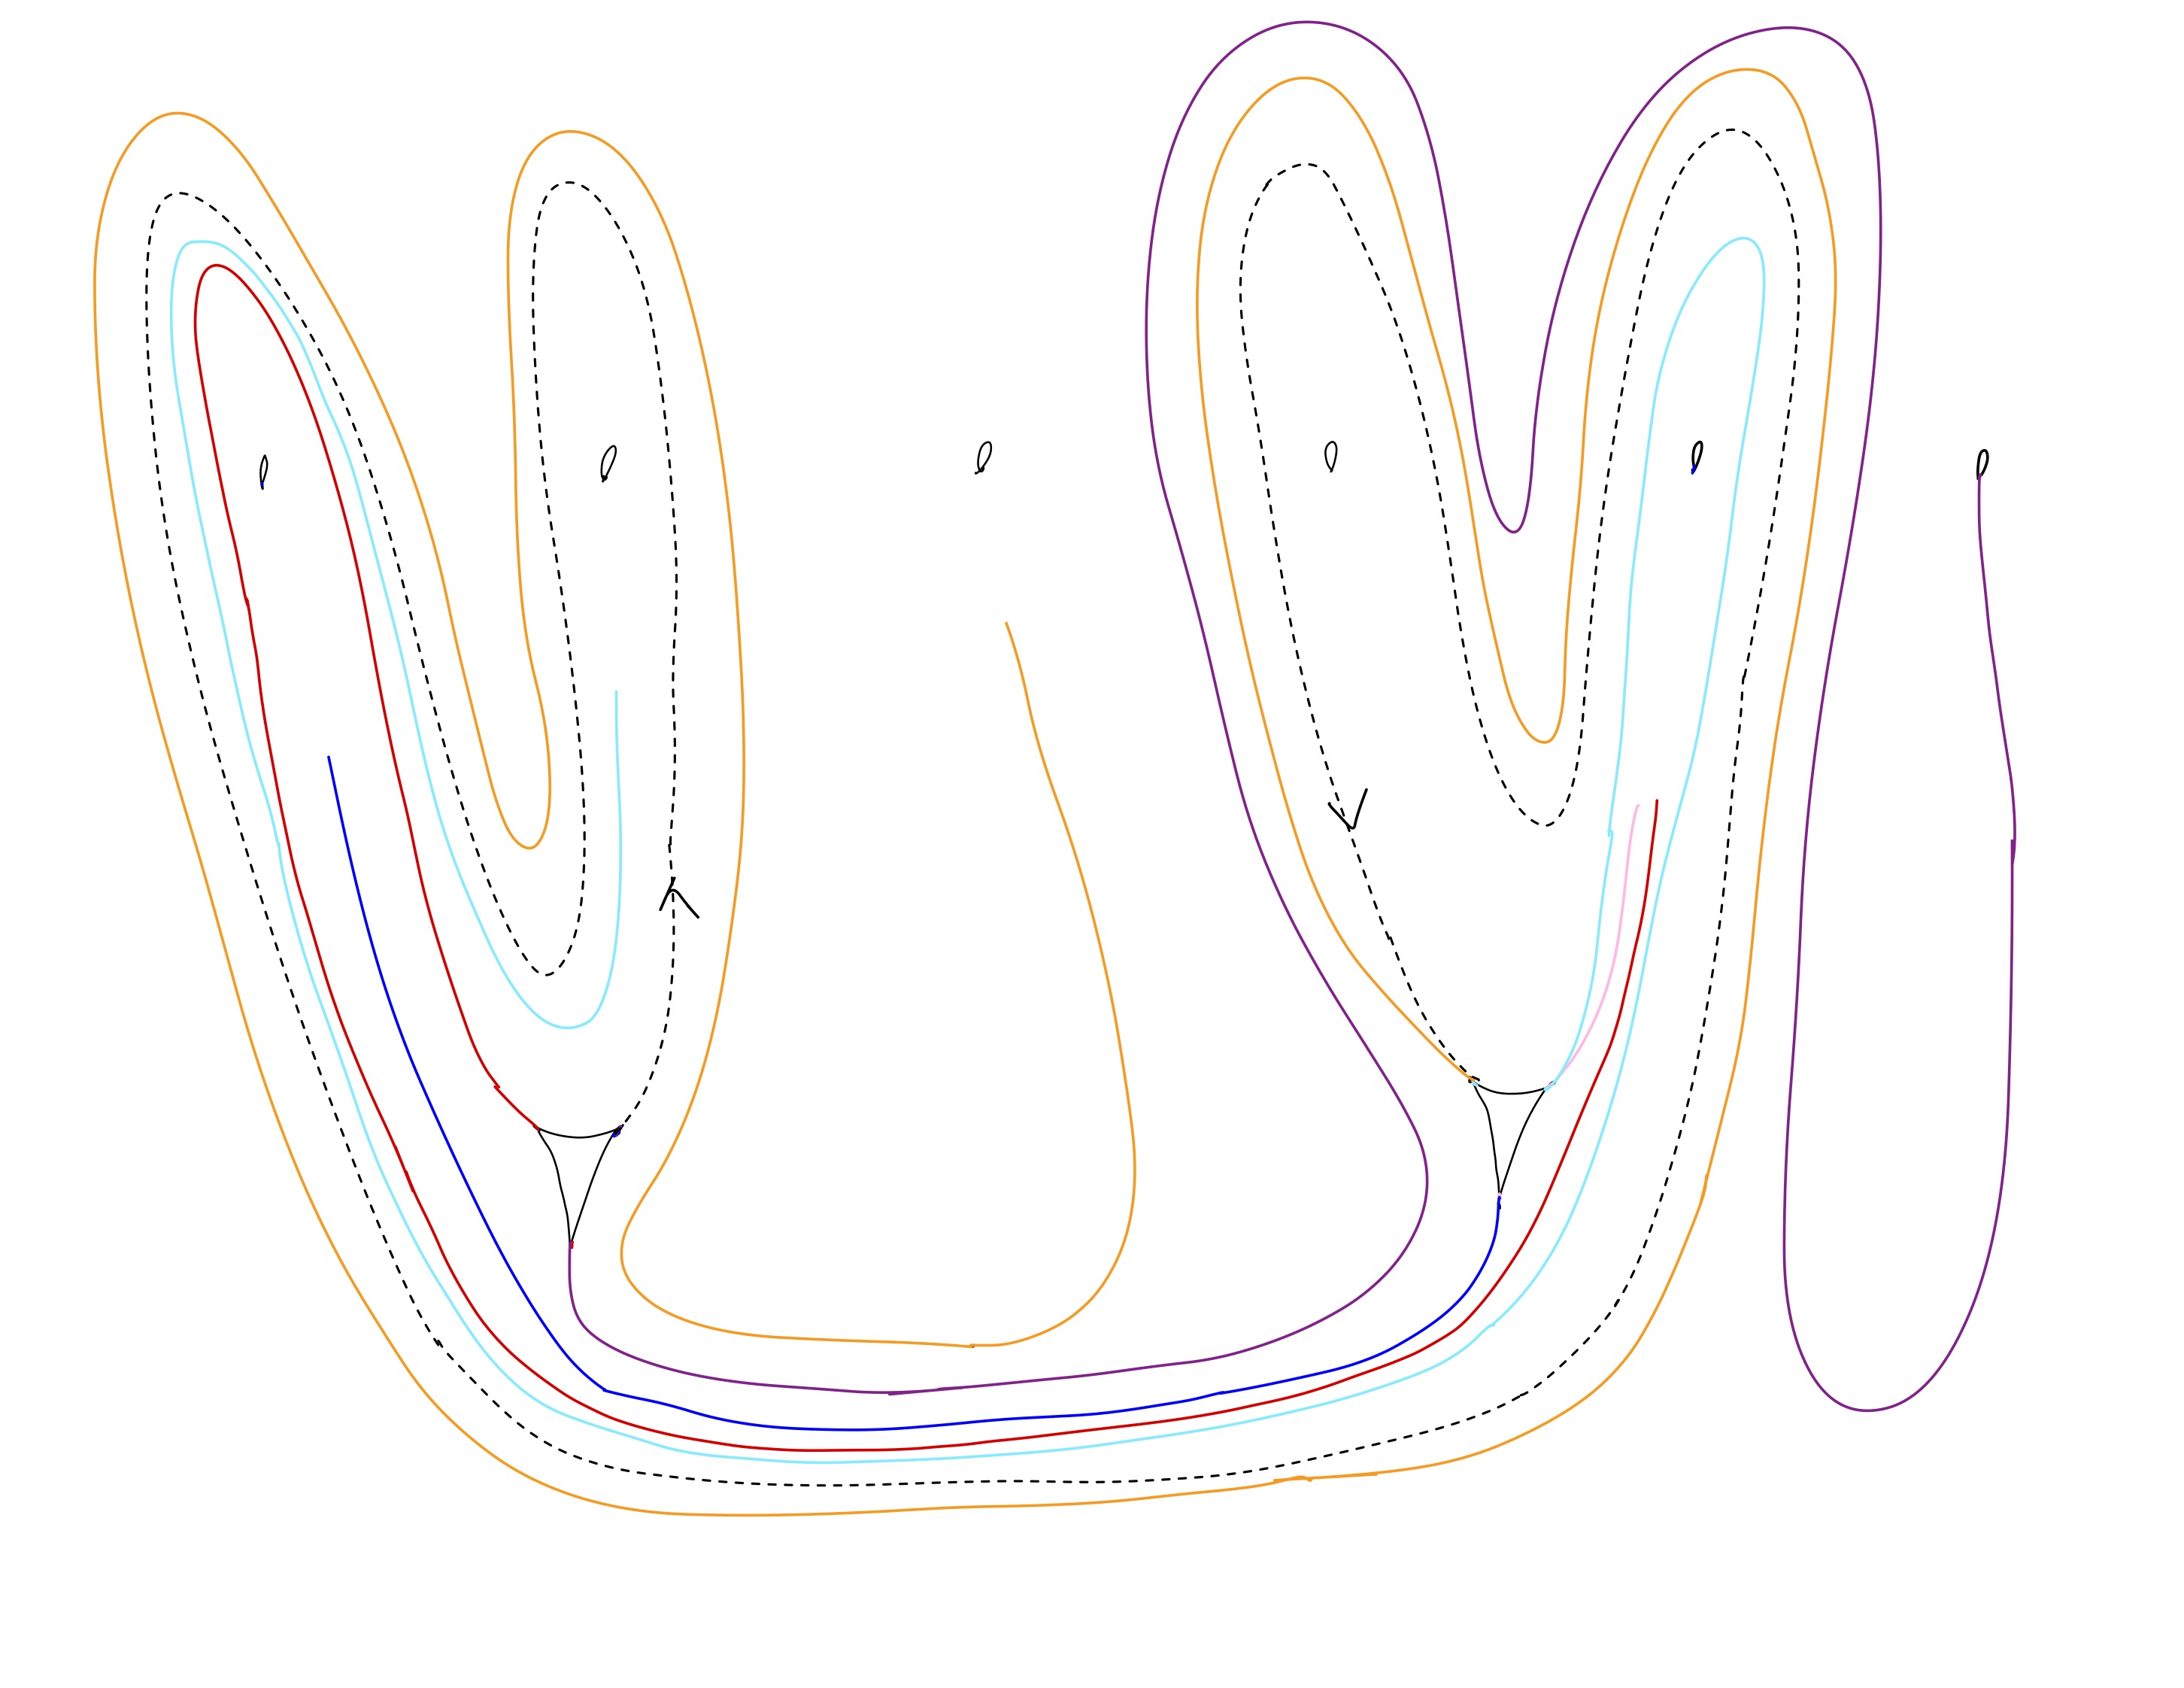
\includegraphics[width=\linewidth]{figures_case_analysis/track17_case_analysis/Gurry-1.jpg}
    \caption{Gurry1}
    \label{fig:Gurry1}
\end{figure}

\begin{figure}[ht]
    \centering
    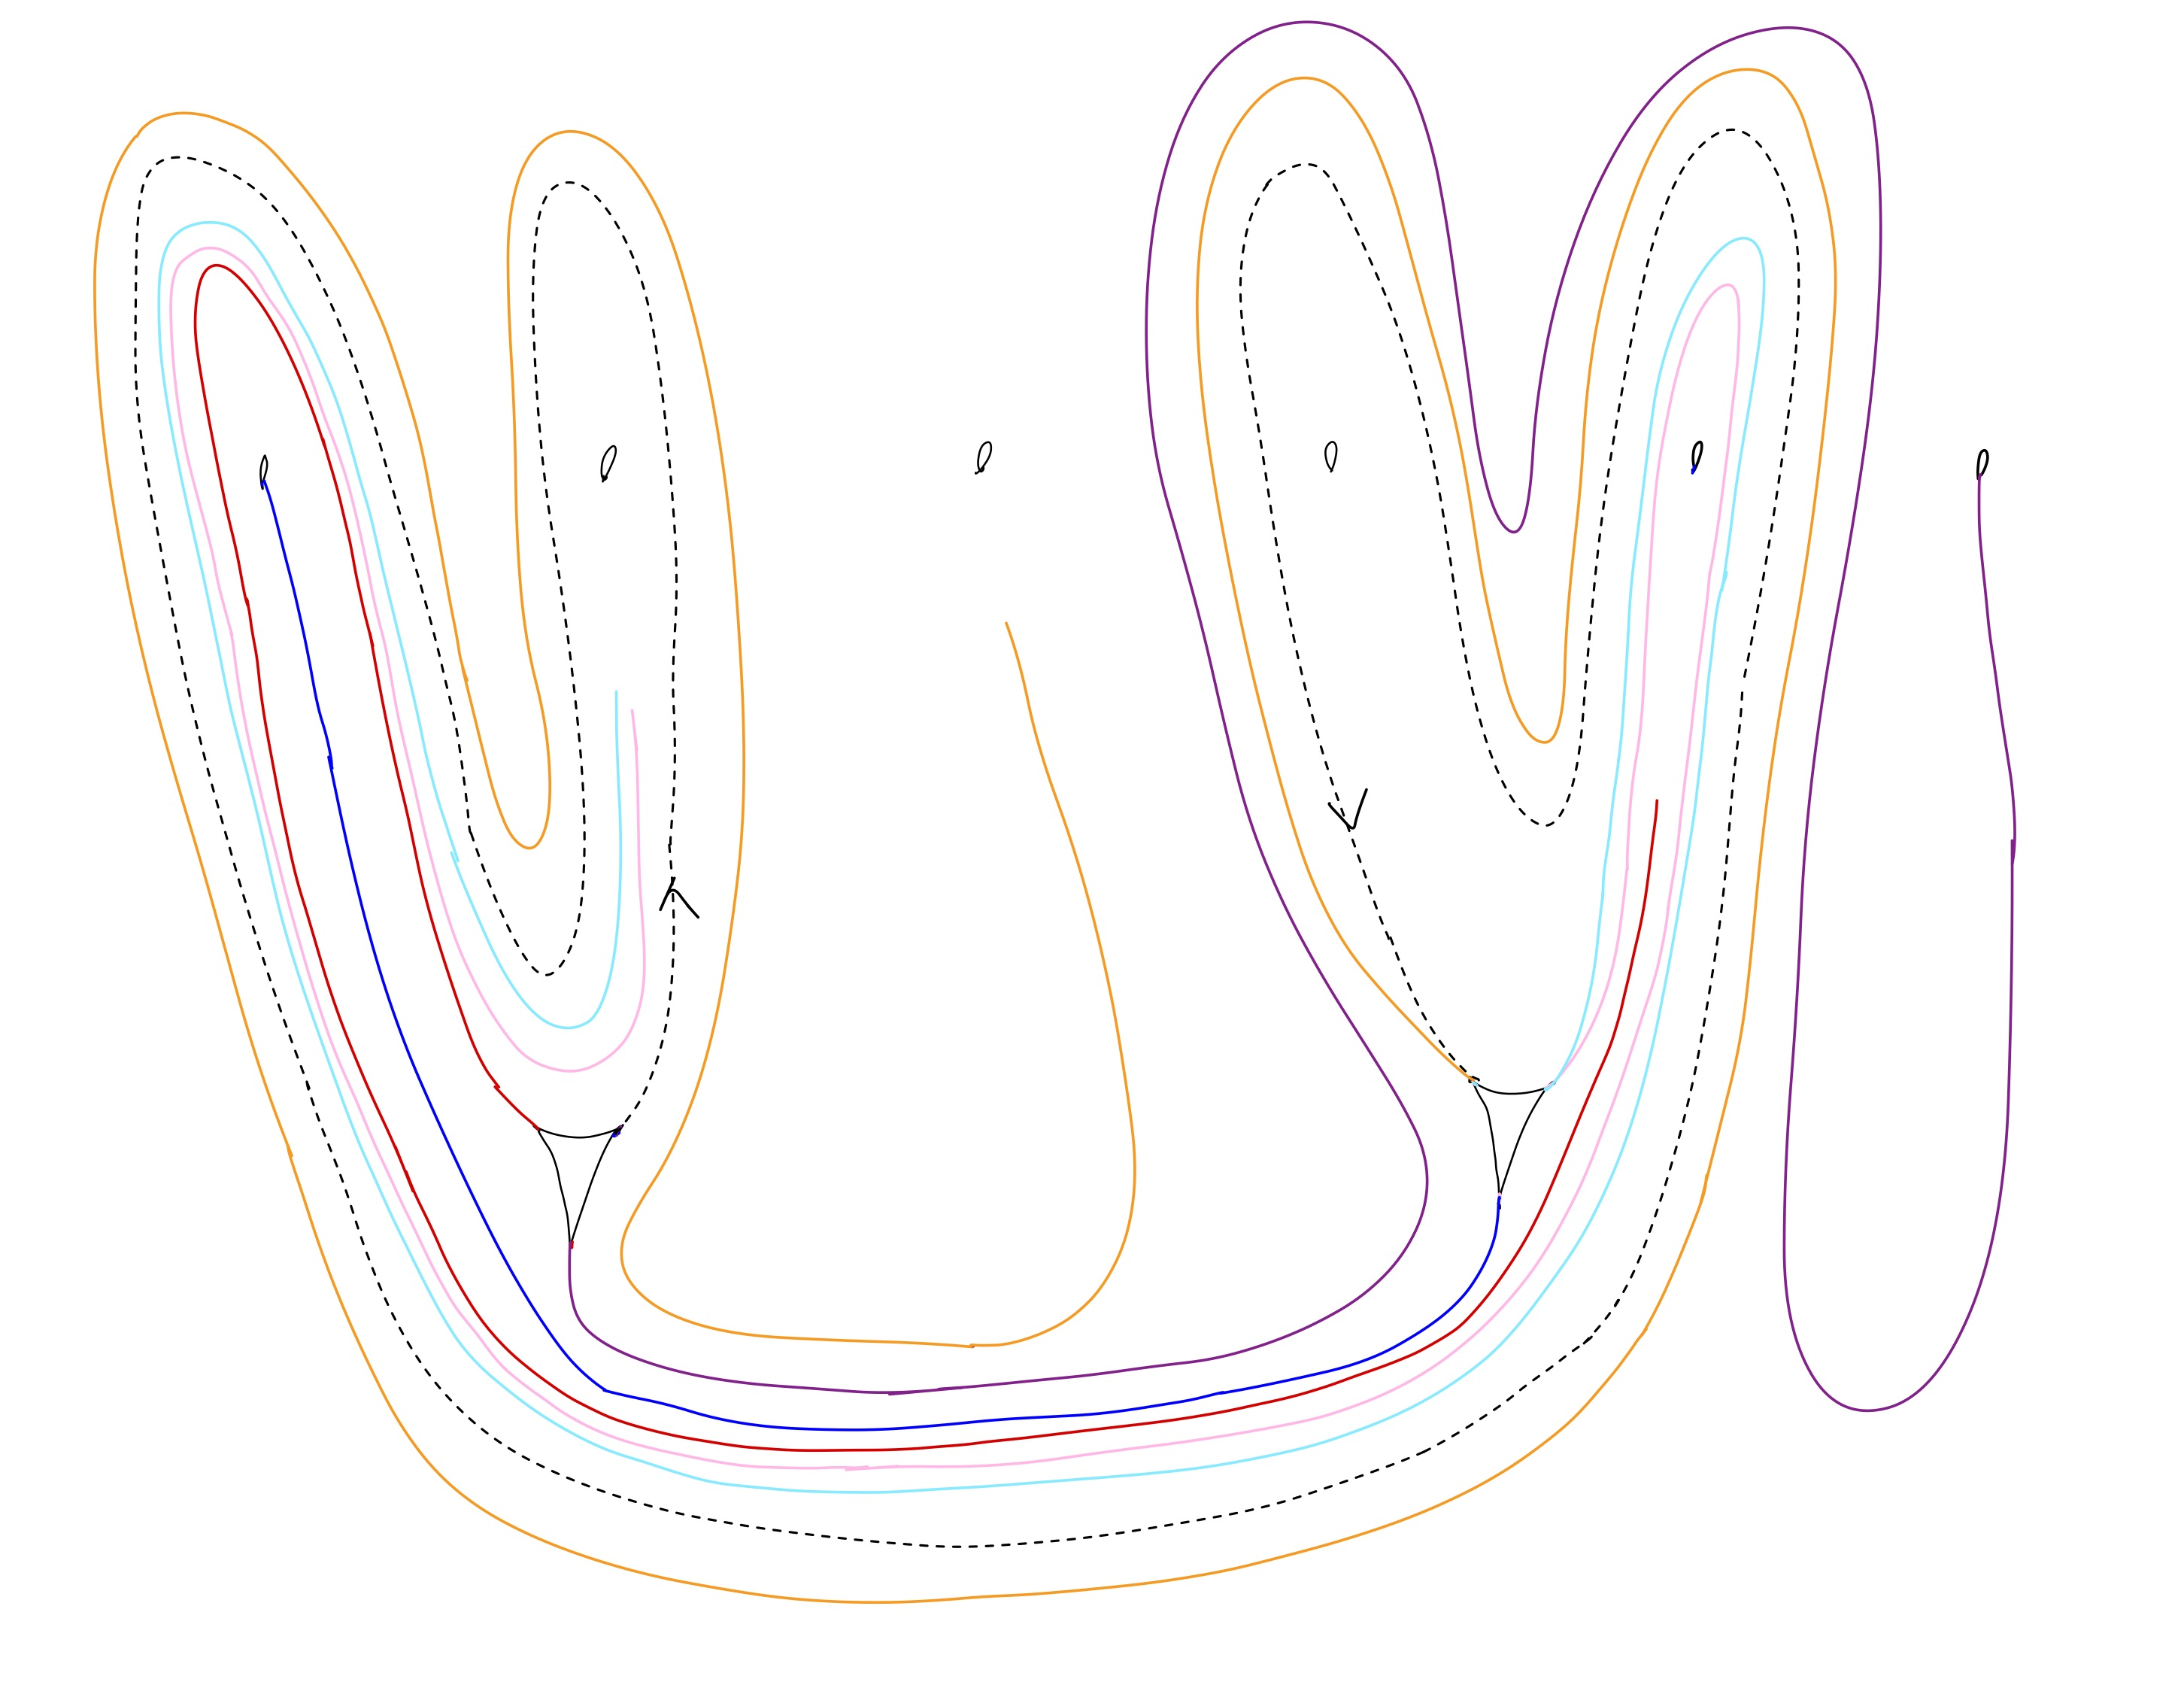
\includegraphics[width=\linewidth]{figures_case_analysis/track17_case_analysis/Gurry-2.jpg}
    \caption{Gurry2}
    \label{fig:Gurry2}
\end{figure}
\clearpage

\begin{figure}[ht]
    \centering
    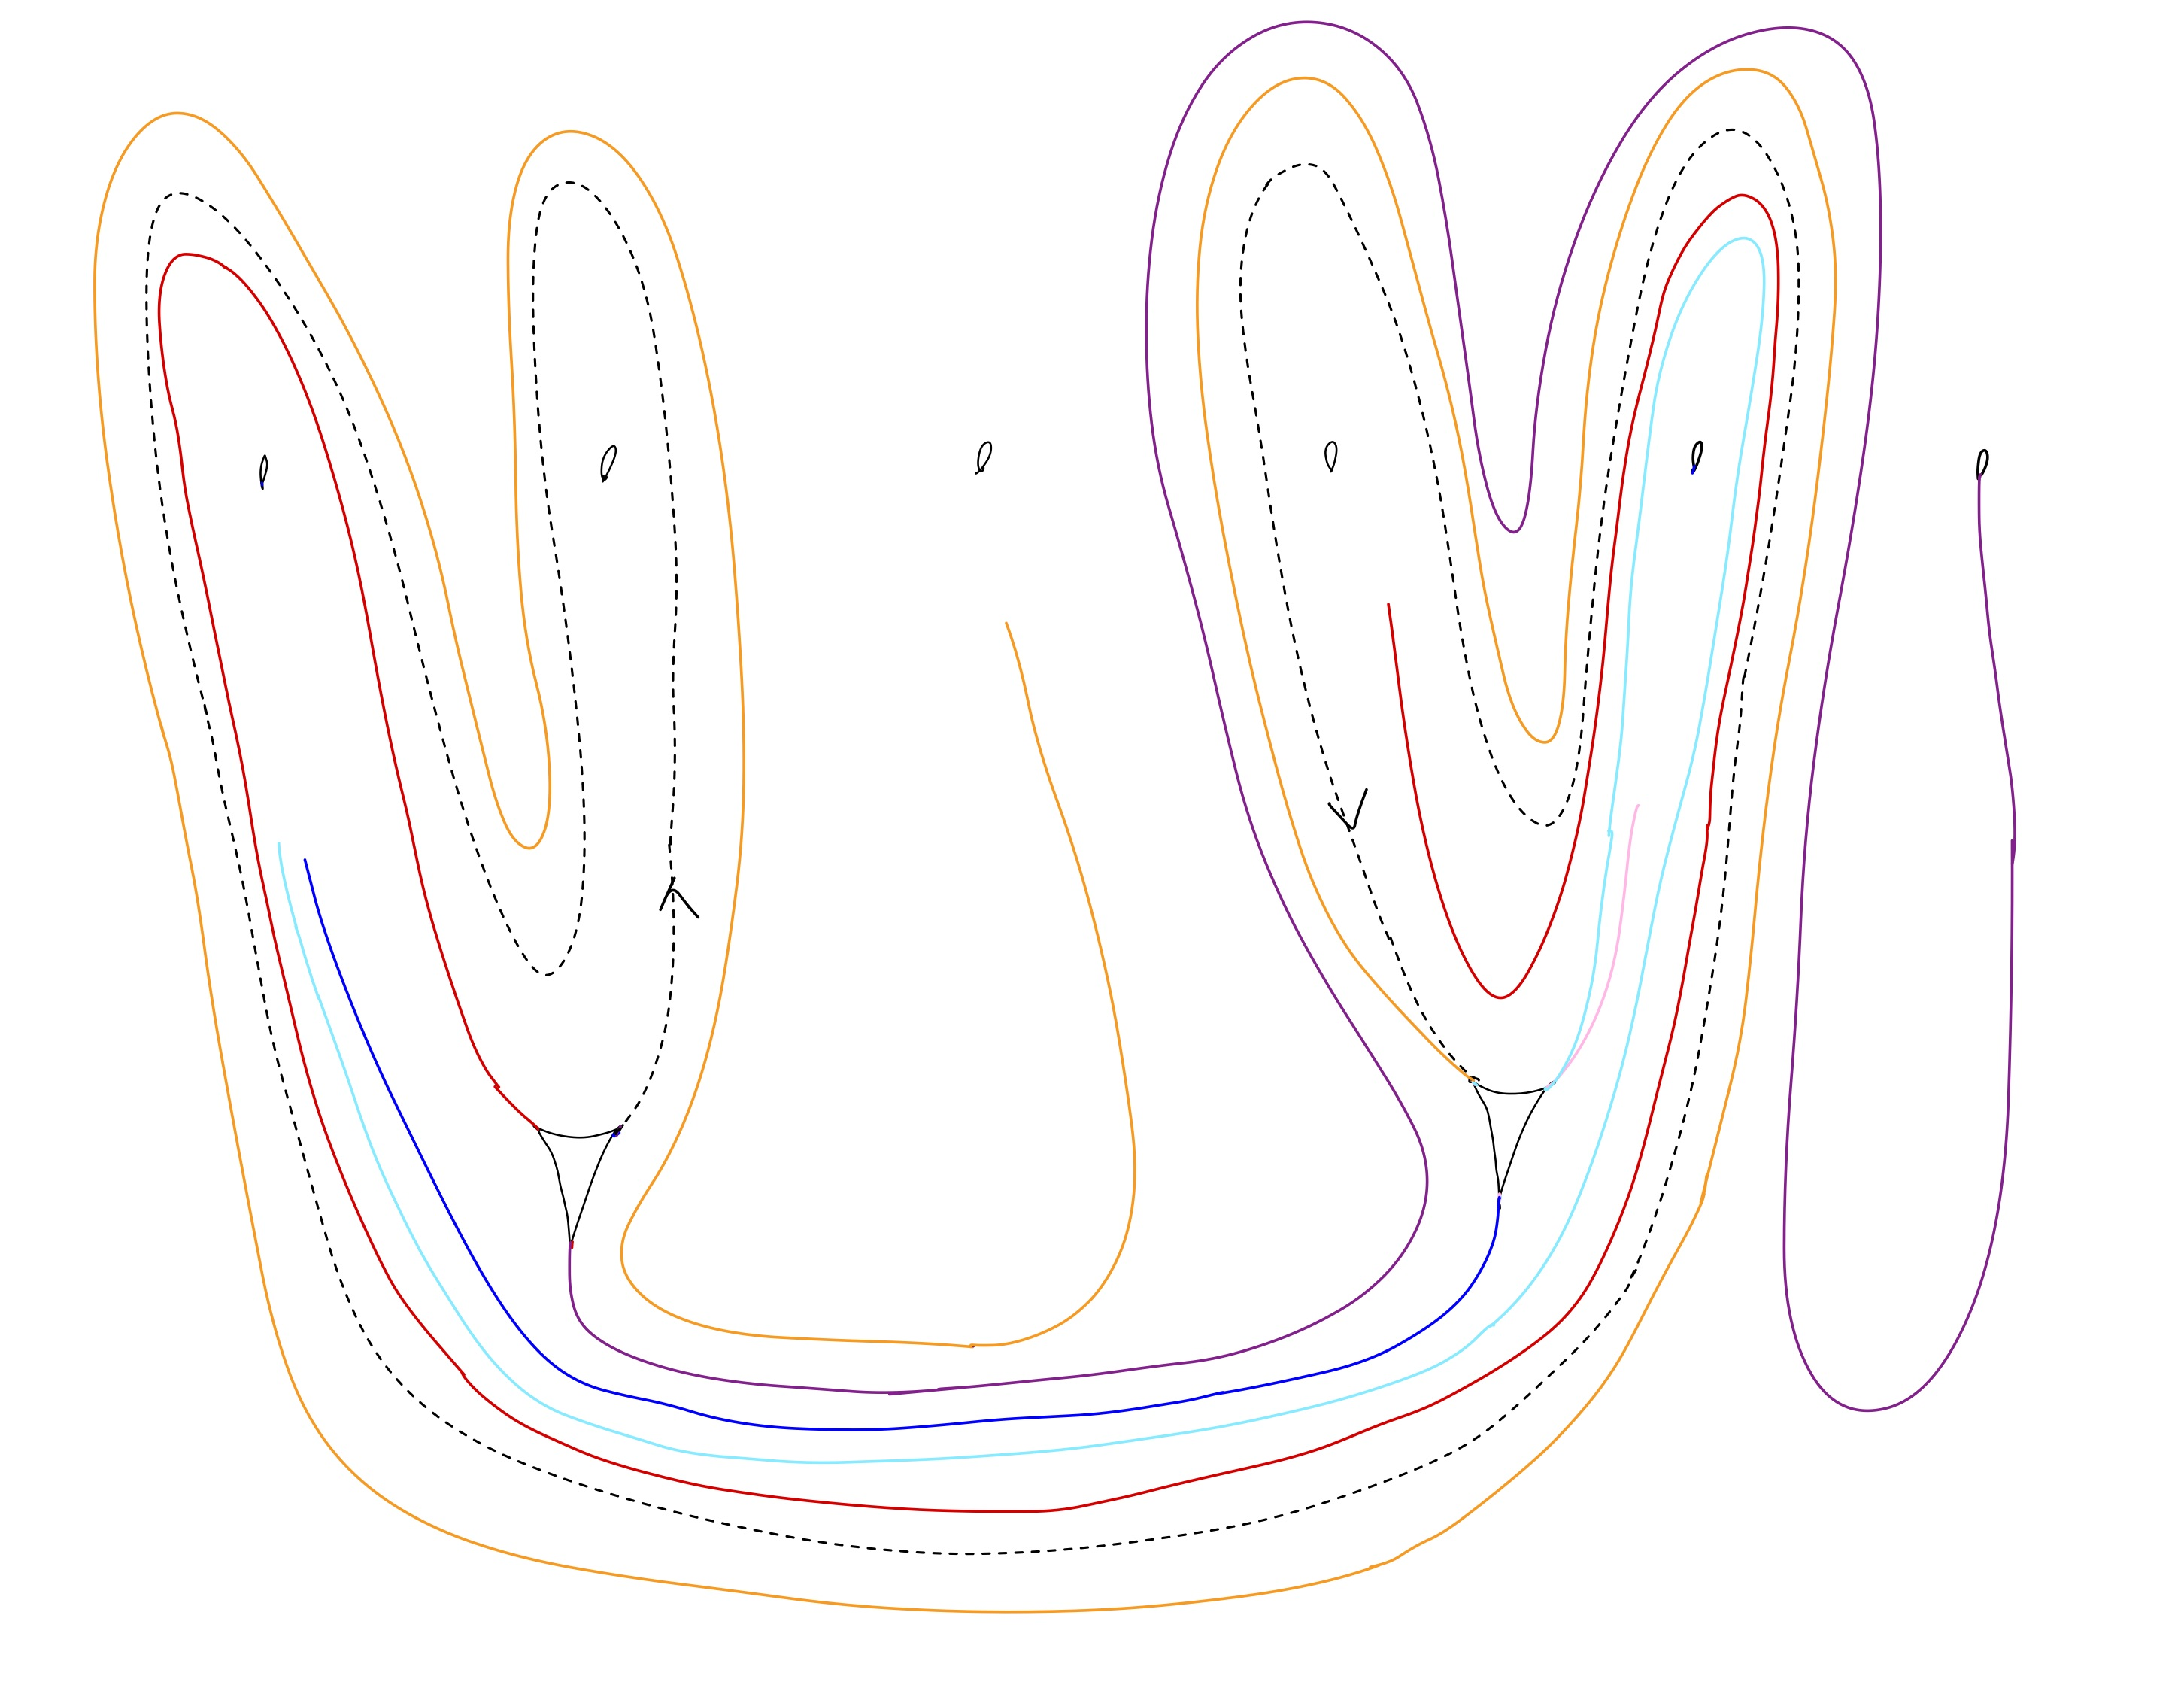
\includegraphics[width=\linewidth]{figures_case_analysis/track17_case_analysis/Hanch.jpg}
    \caption{Hanch1}
    \label{fig:Hanch1}
\end{figure}
\clearpage

\begin{figure}[ht]
    \centering
    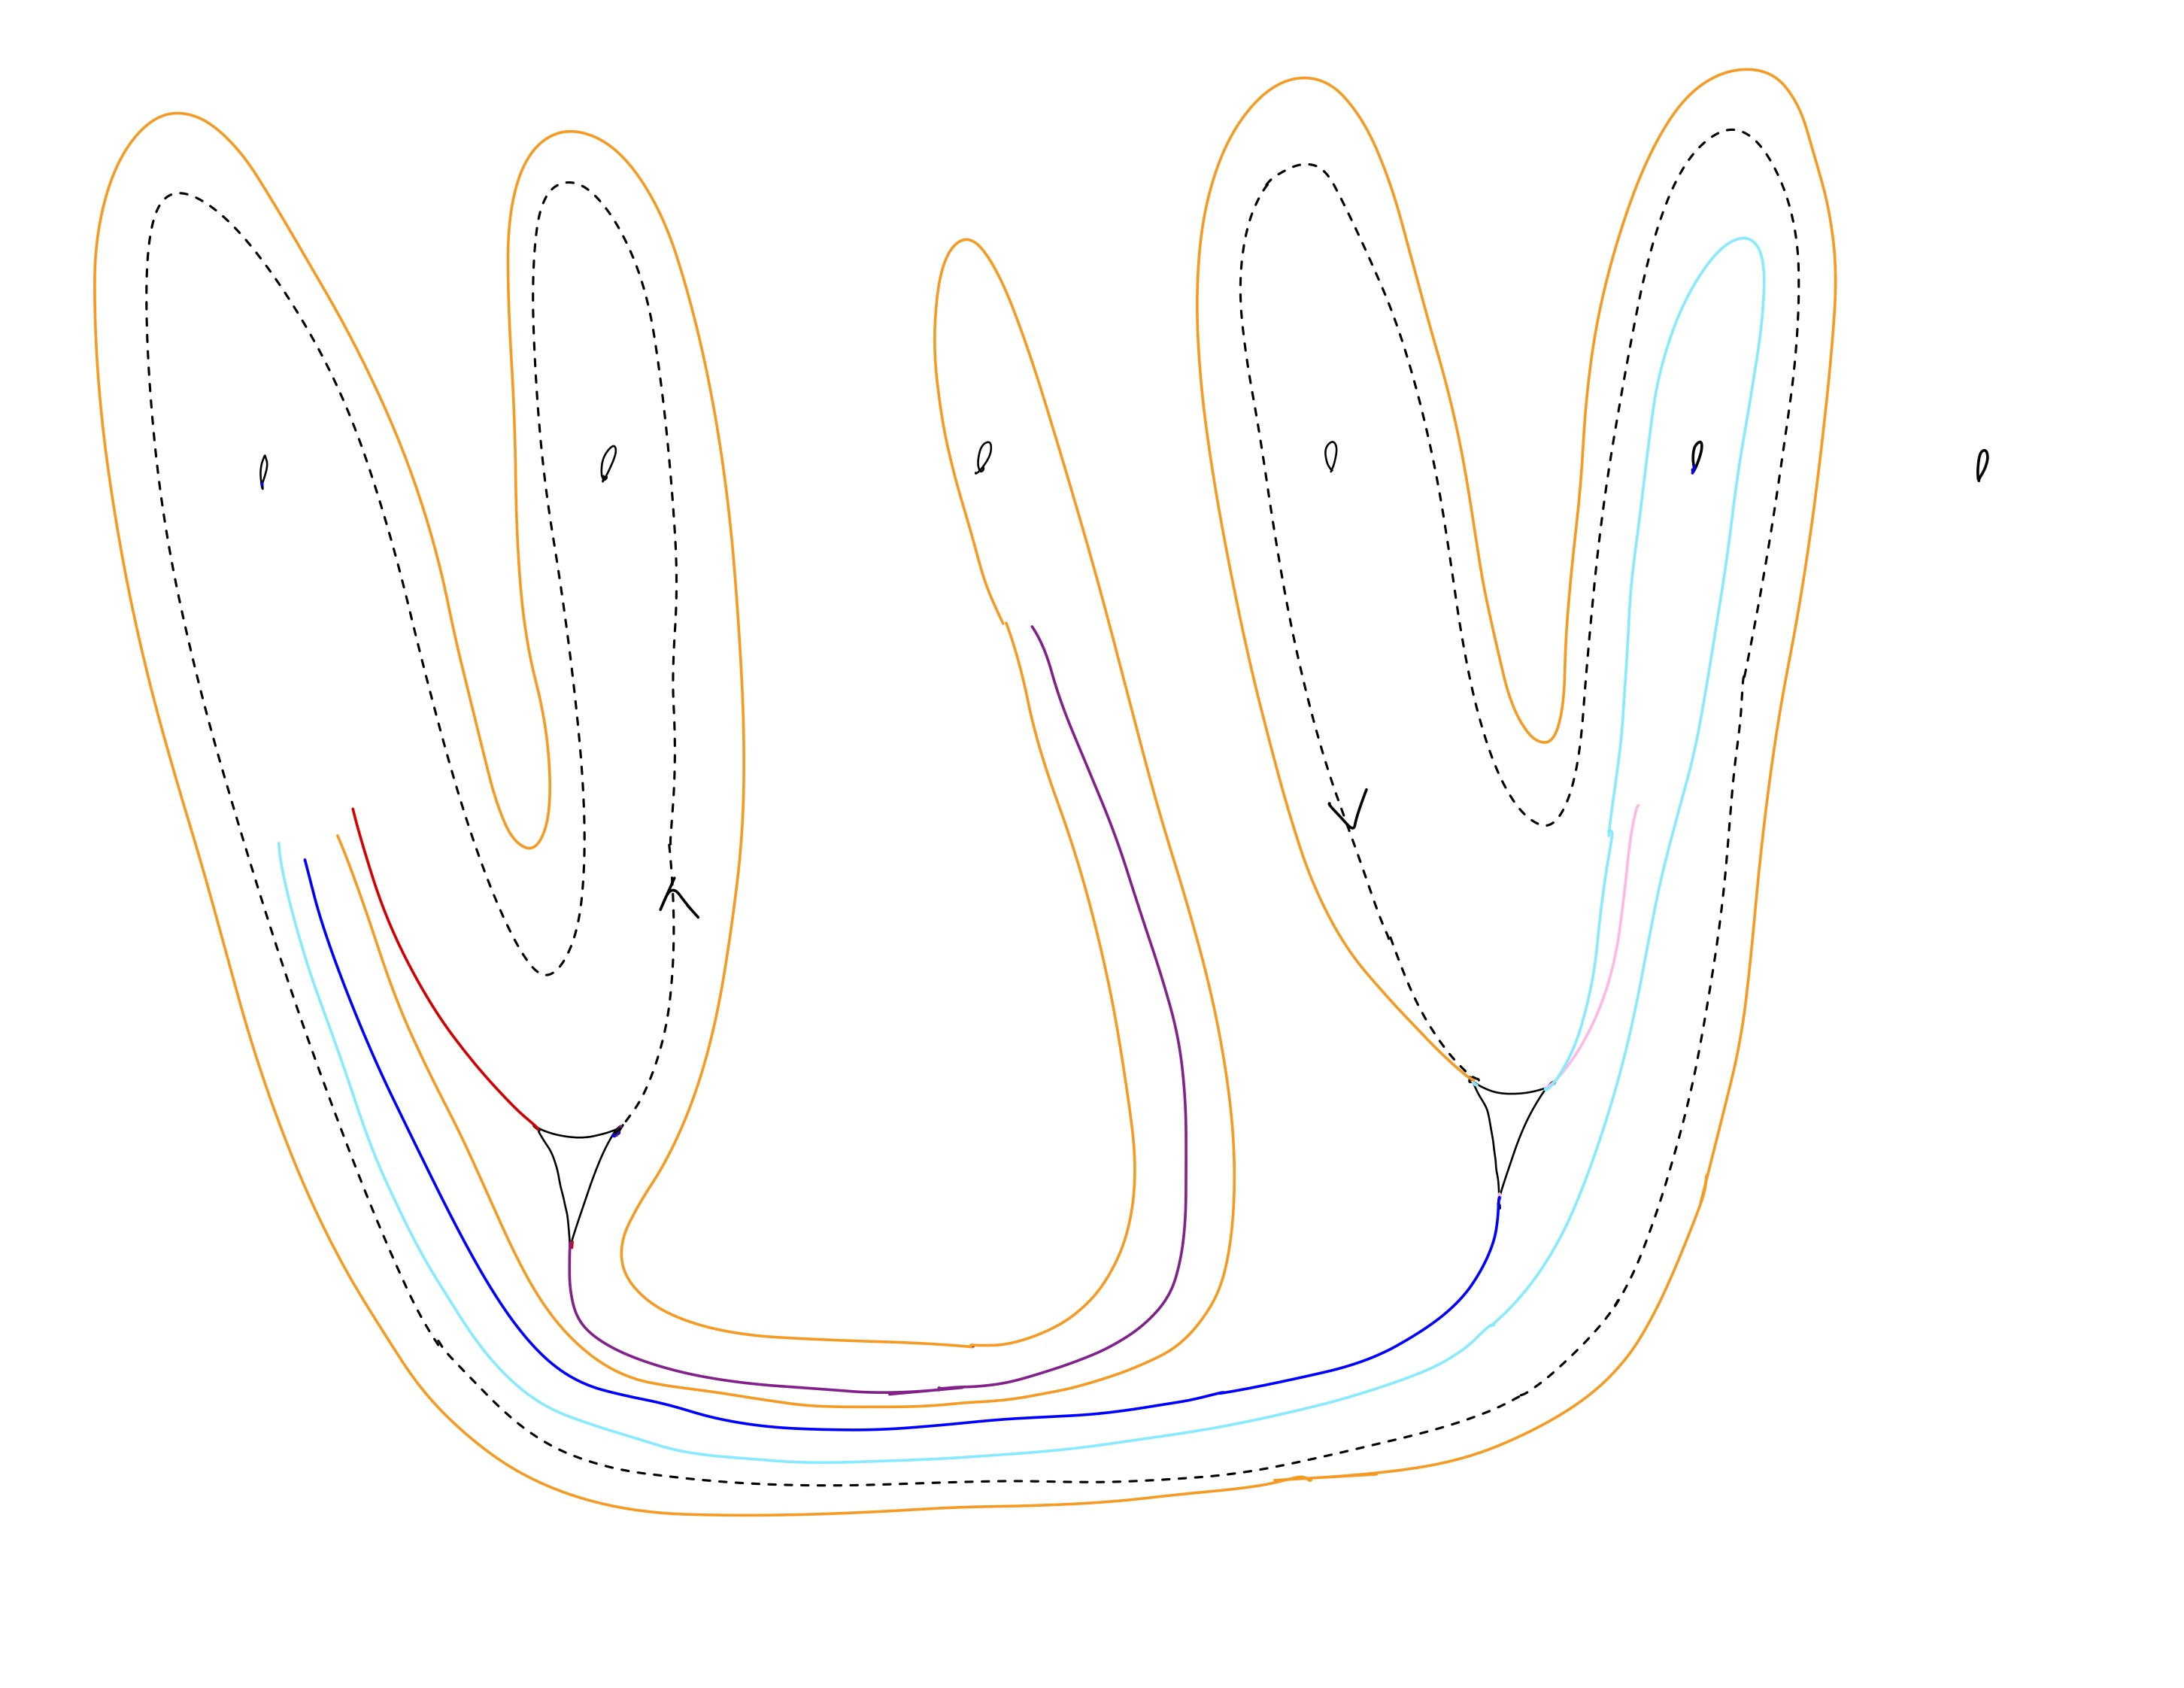
\includegraphics[width=\linewidth]{figures_case_analysis/track17_case_analysis/Roop-01.jpg}
    \caption{Roop1}
    \label{fig:Roop1}
\end{figure}

\begin{figure}[ht]
    \centering
    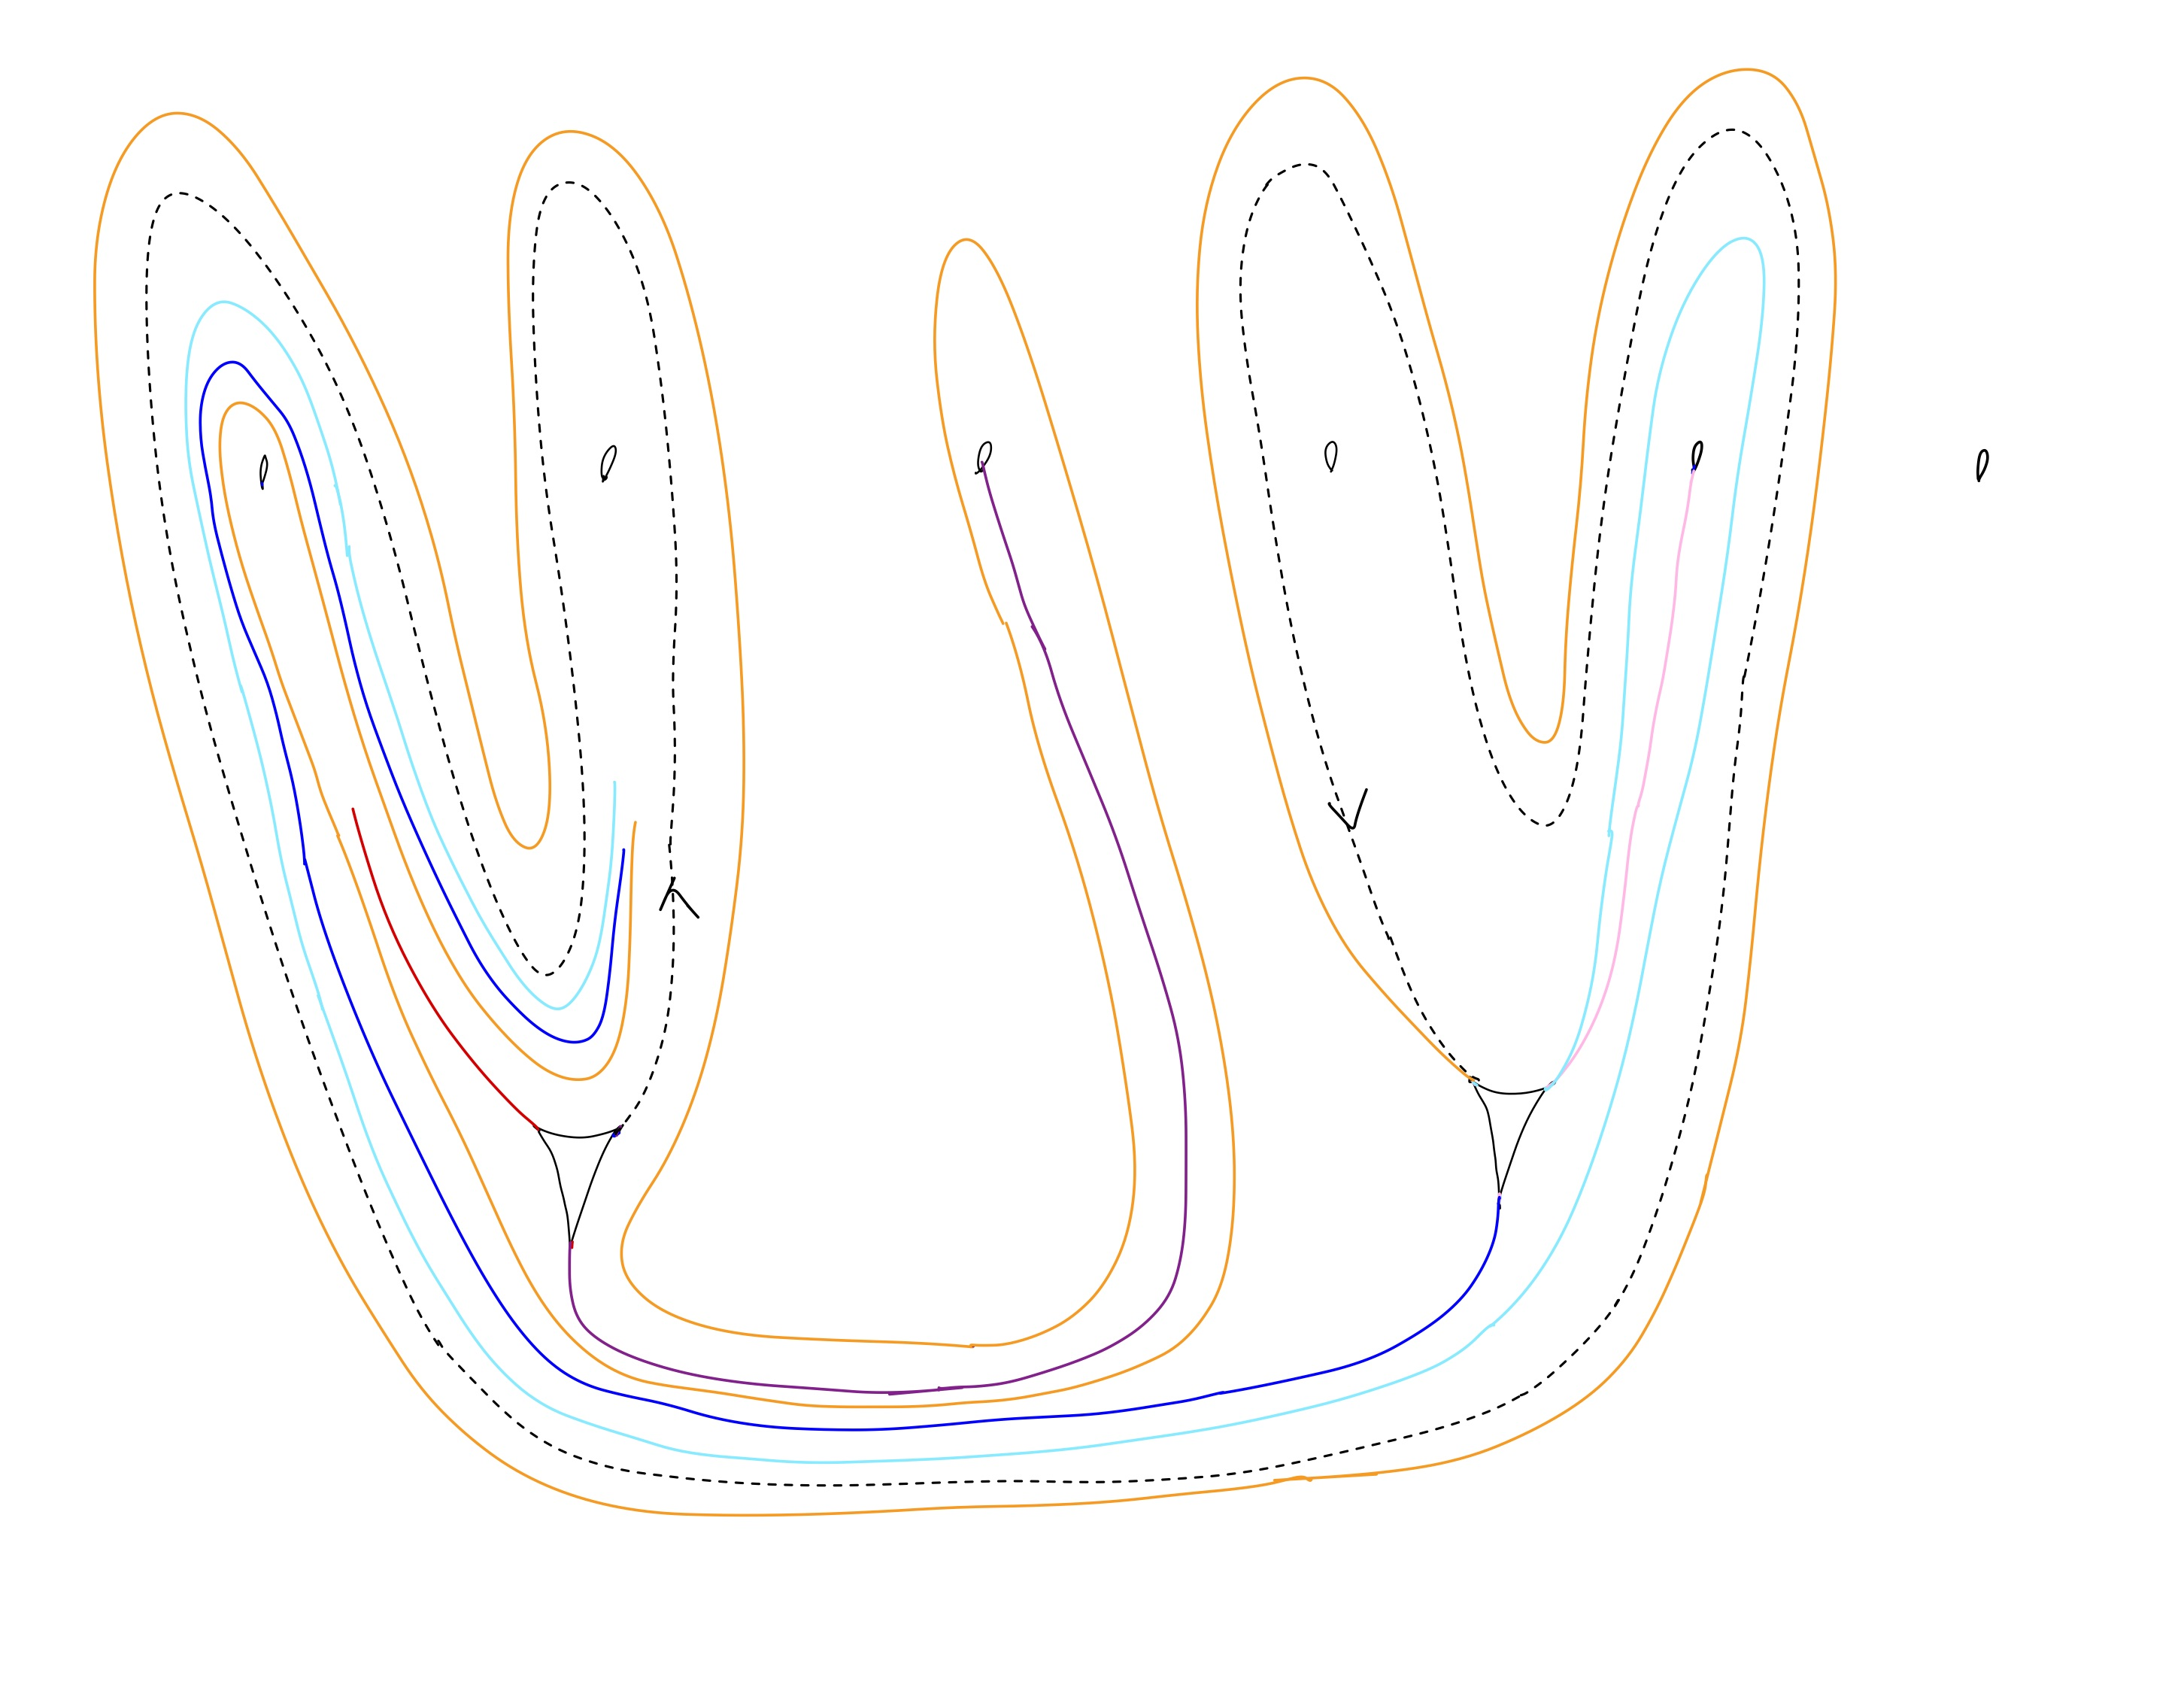
\includegraphics[width=\linewidth]{figures_case_analysis/track17_case_analysis/Roop-02.jpg}
    \caption{Roop2}
    \label{fig:Roop2}
\end{figure}

\begin{figure}[ht]
    \centering
    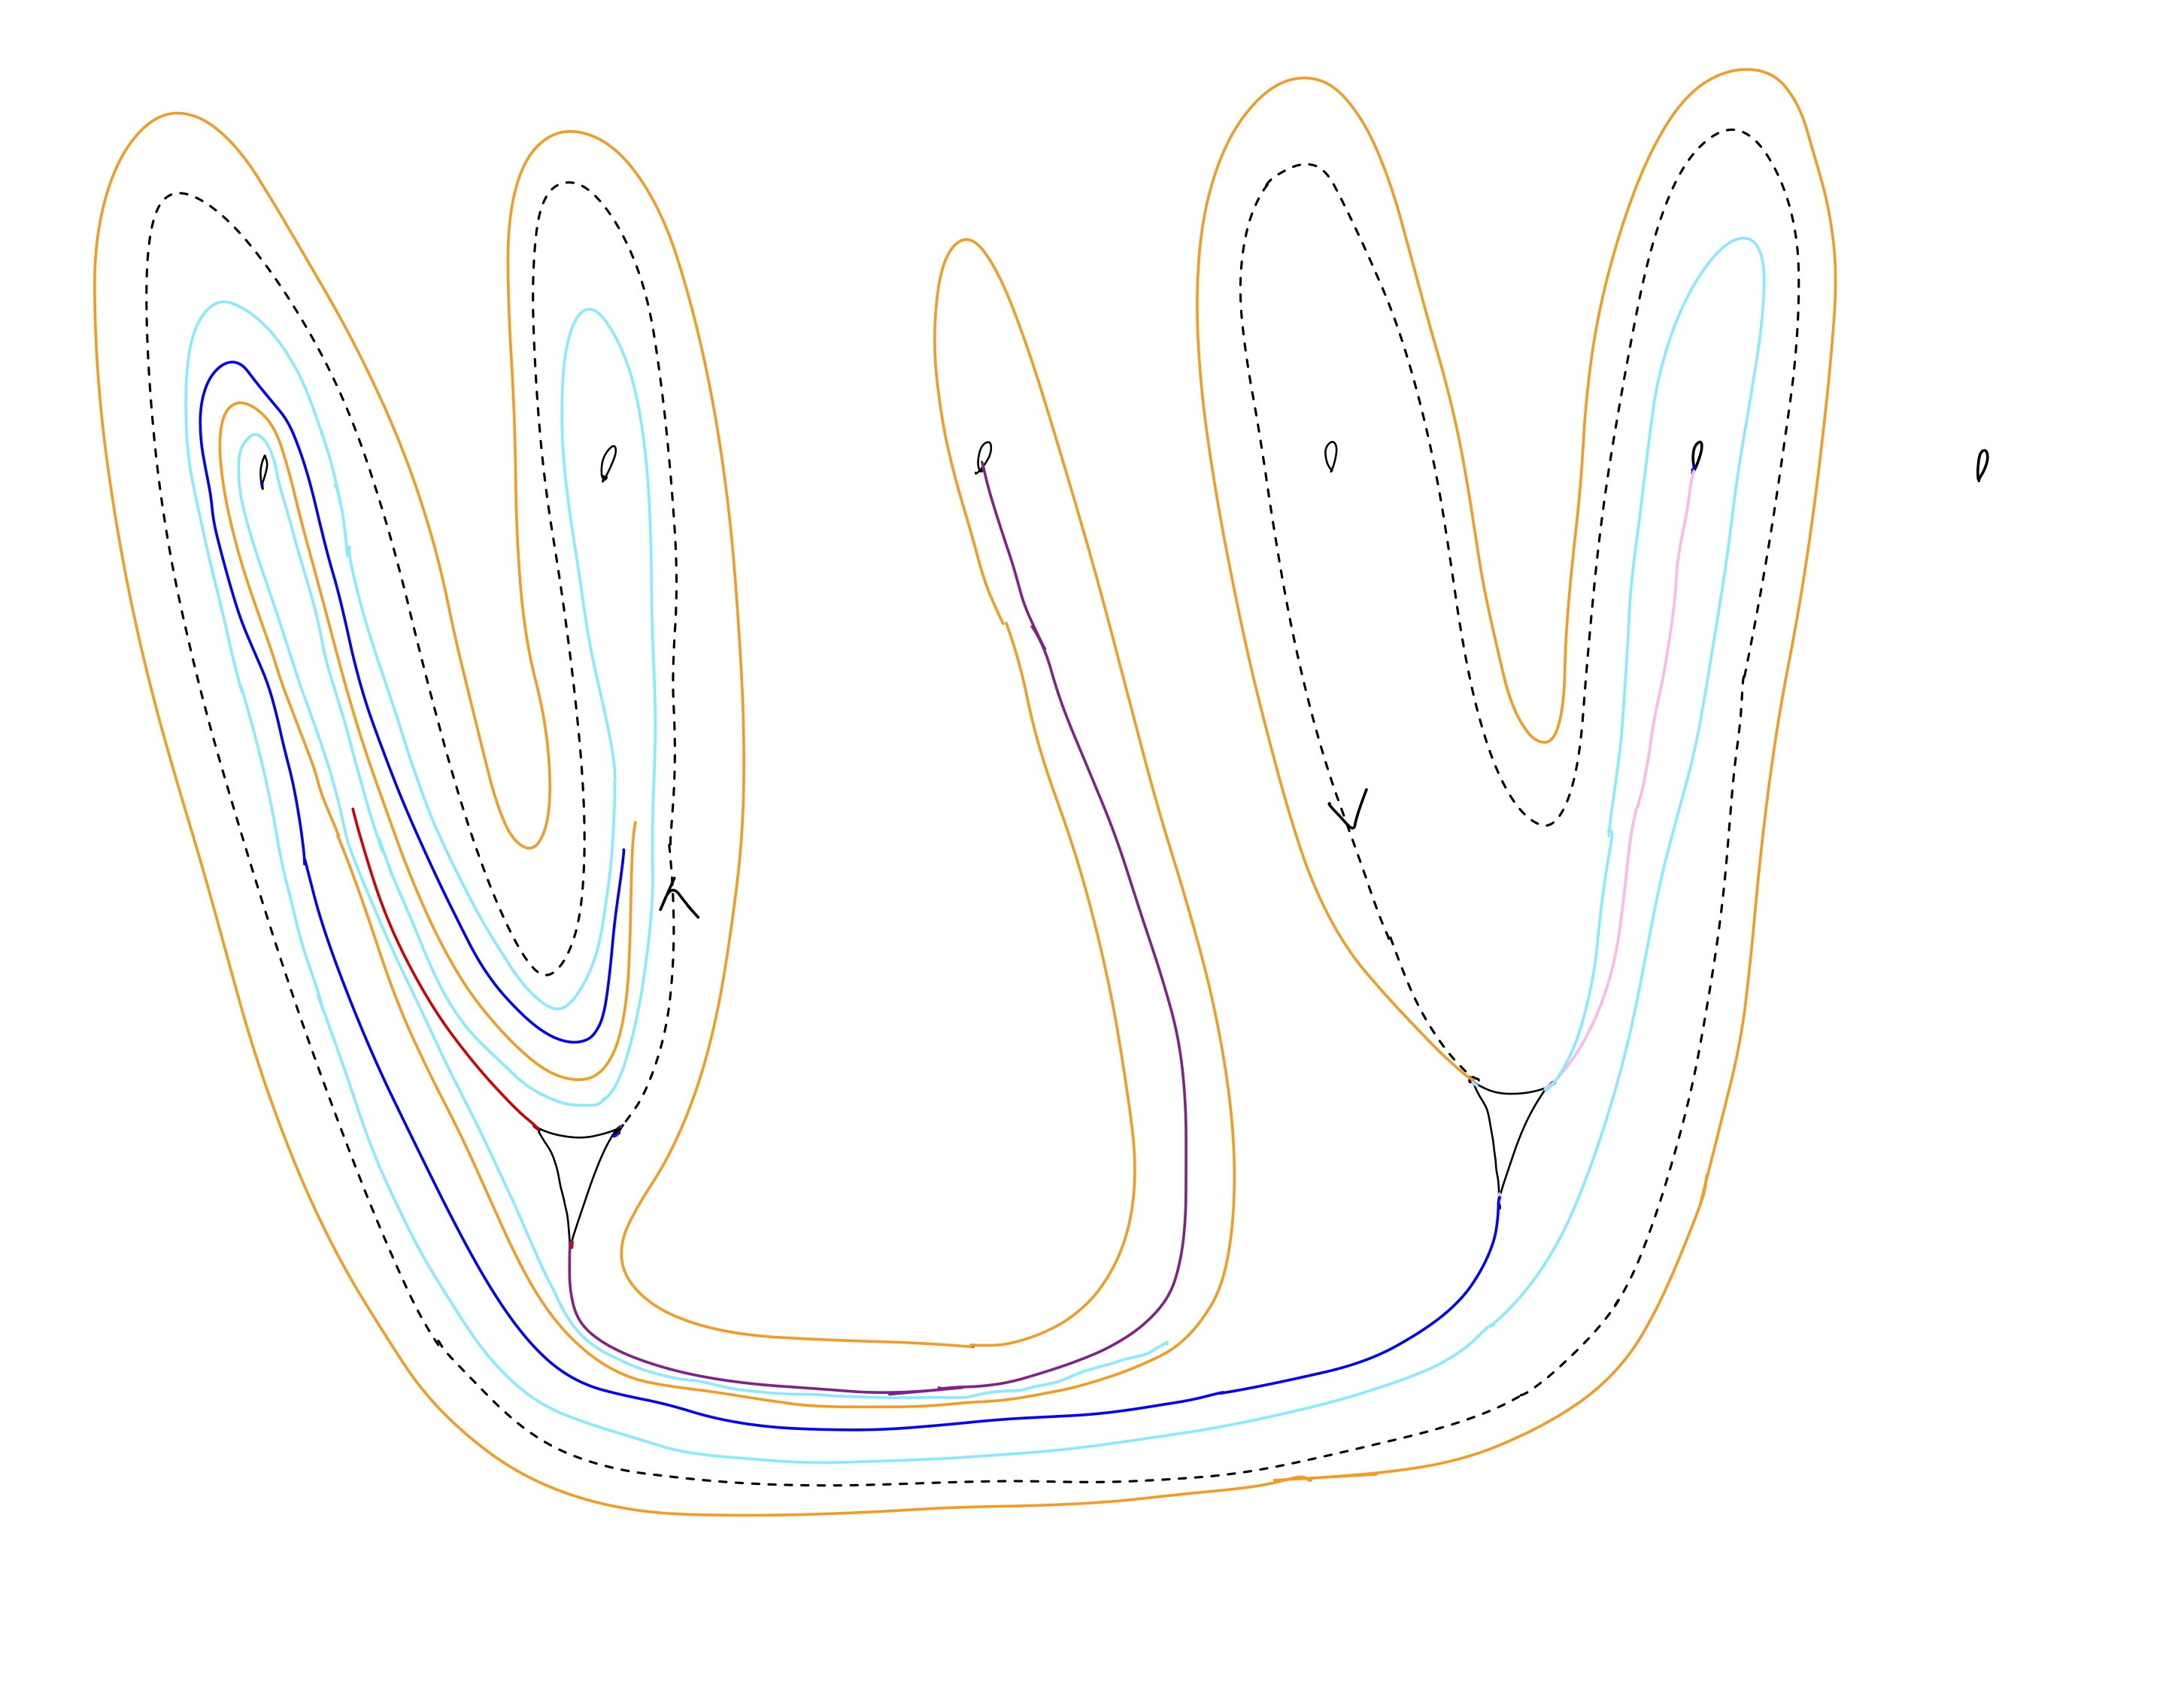
\includegraphics[width=\linewidth]{figures_case_analysis/track17_case_analysis/Roop-03.jpg}
    \caption{Roop3}
    \label{fig:Roop3}
\end{figure}

\begin{figure}[ht]
    \centering
    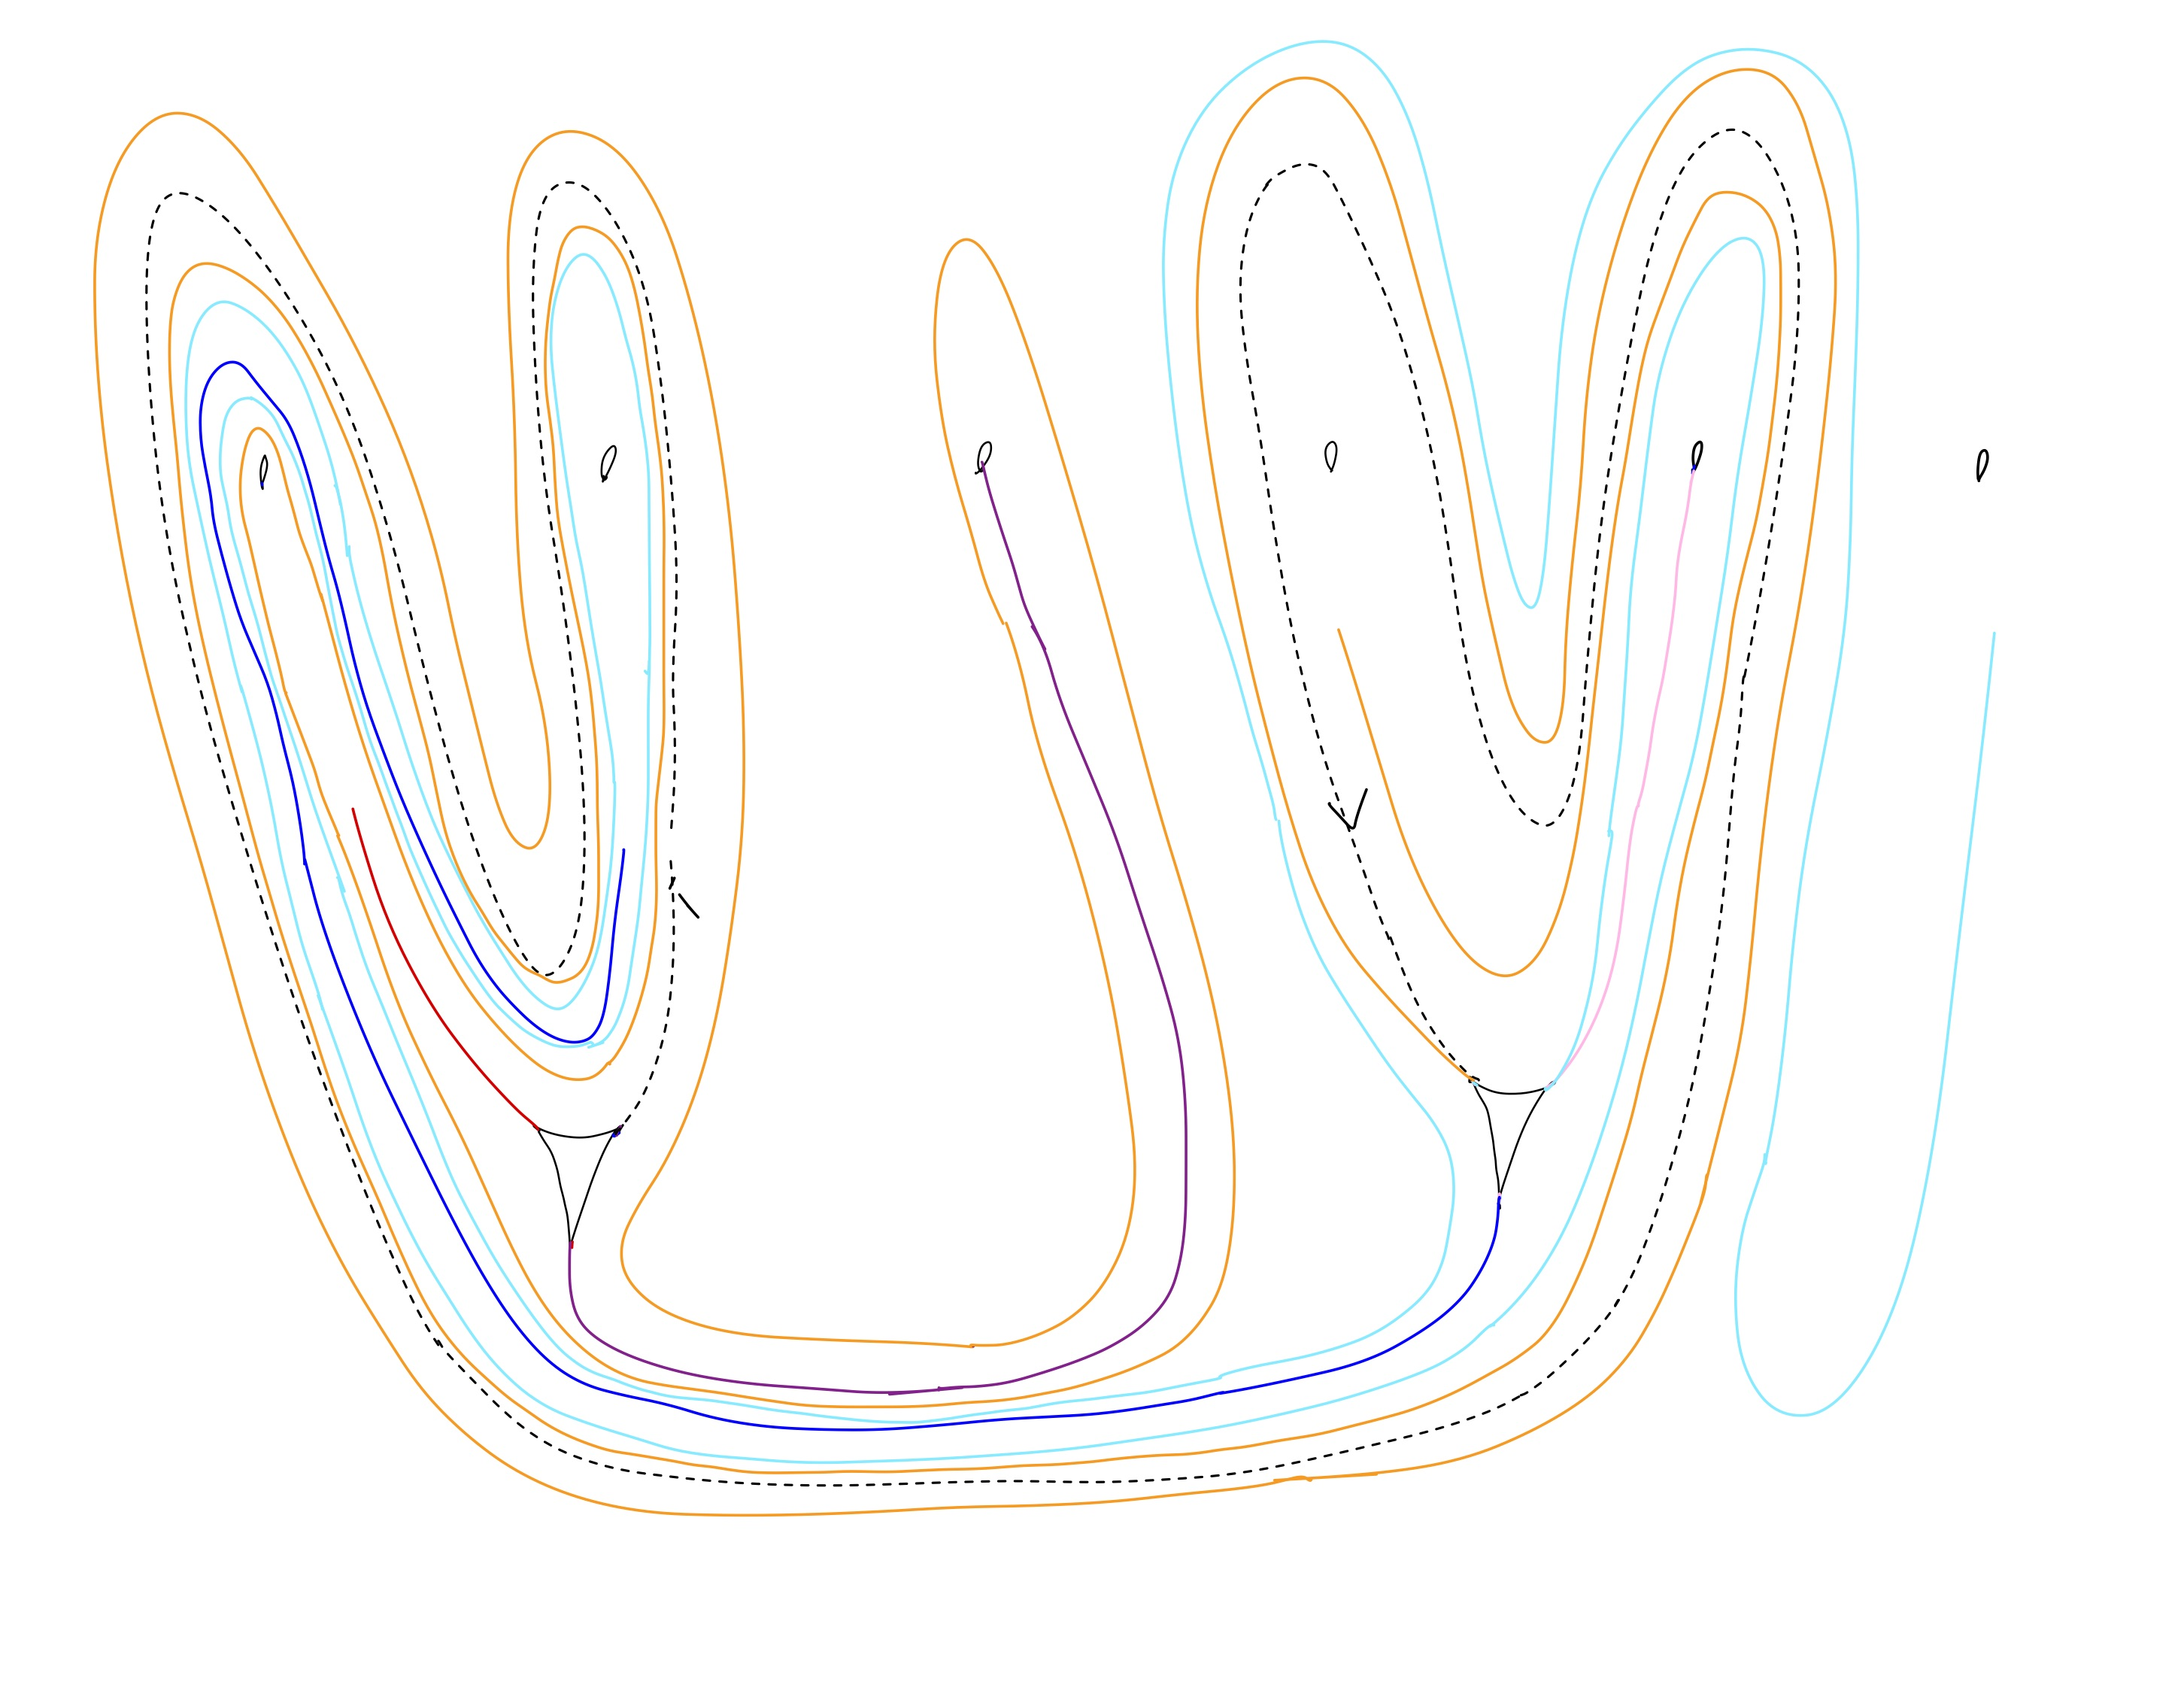
\includegraphics[width=\linewidth]{figures_case_analysis/track17_case_analysis/Roop-04.jpg}
    \caption{Roop4}
    \label{fig:Roop4}
\end{figure}

\begin{figure}[ht]
    \centering
    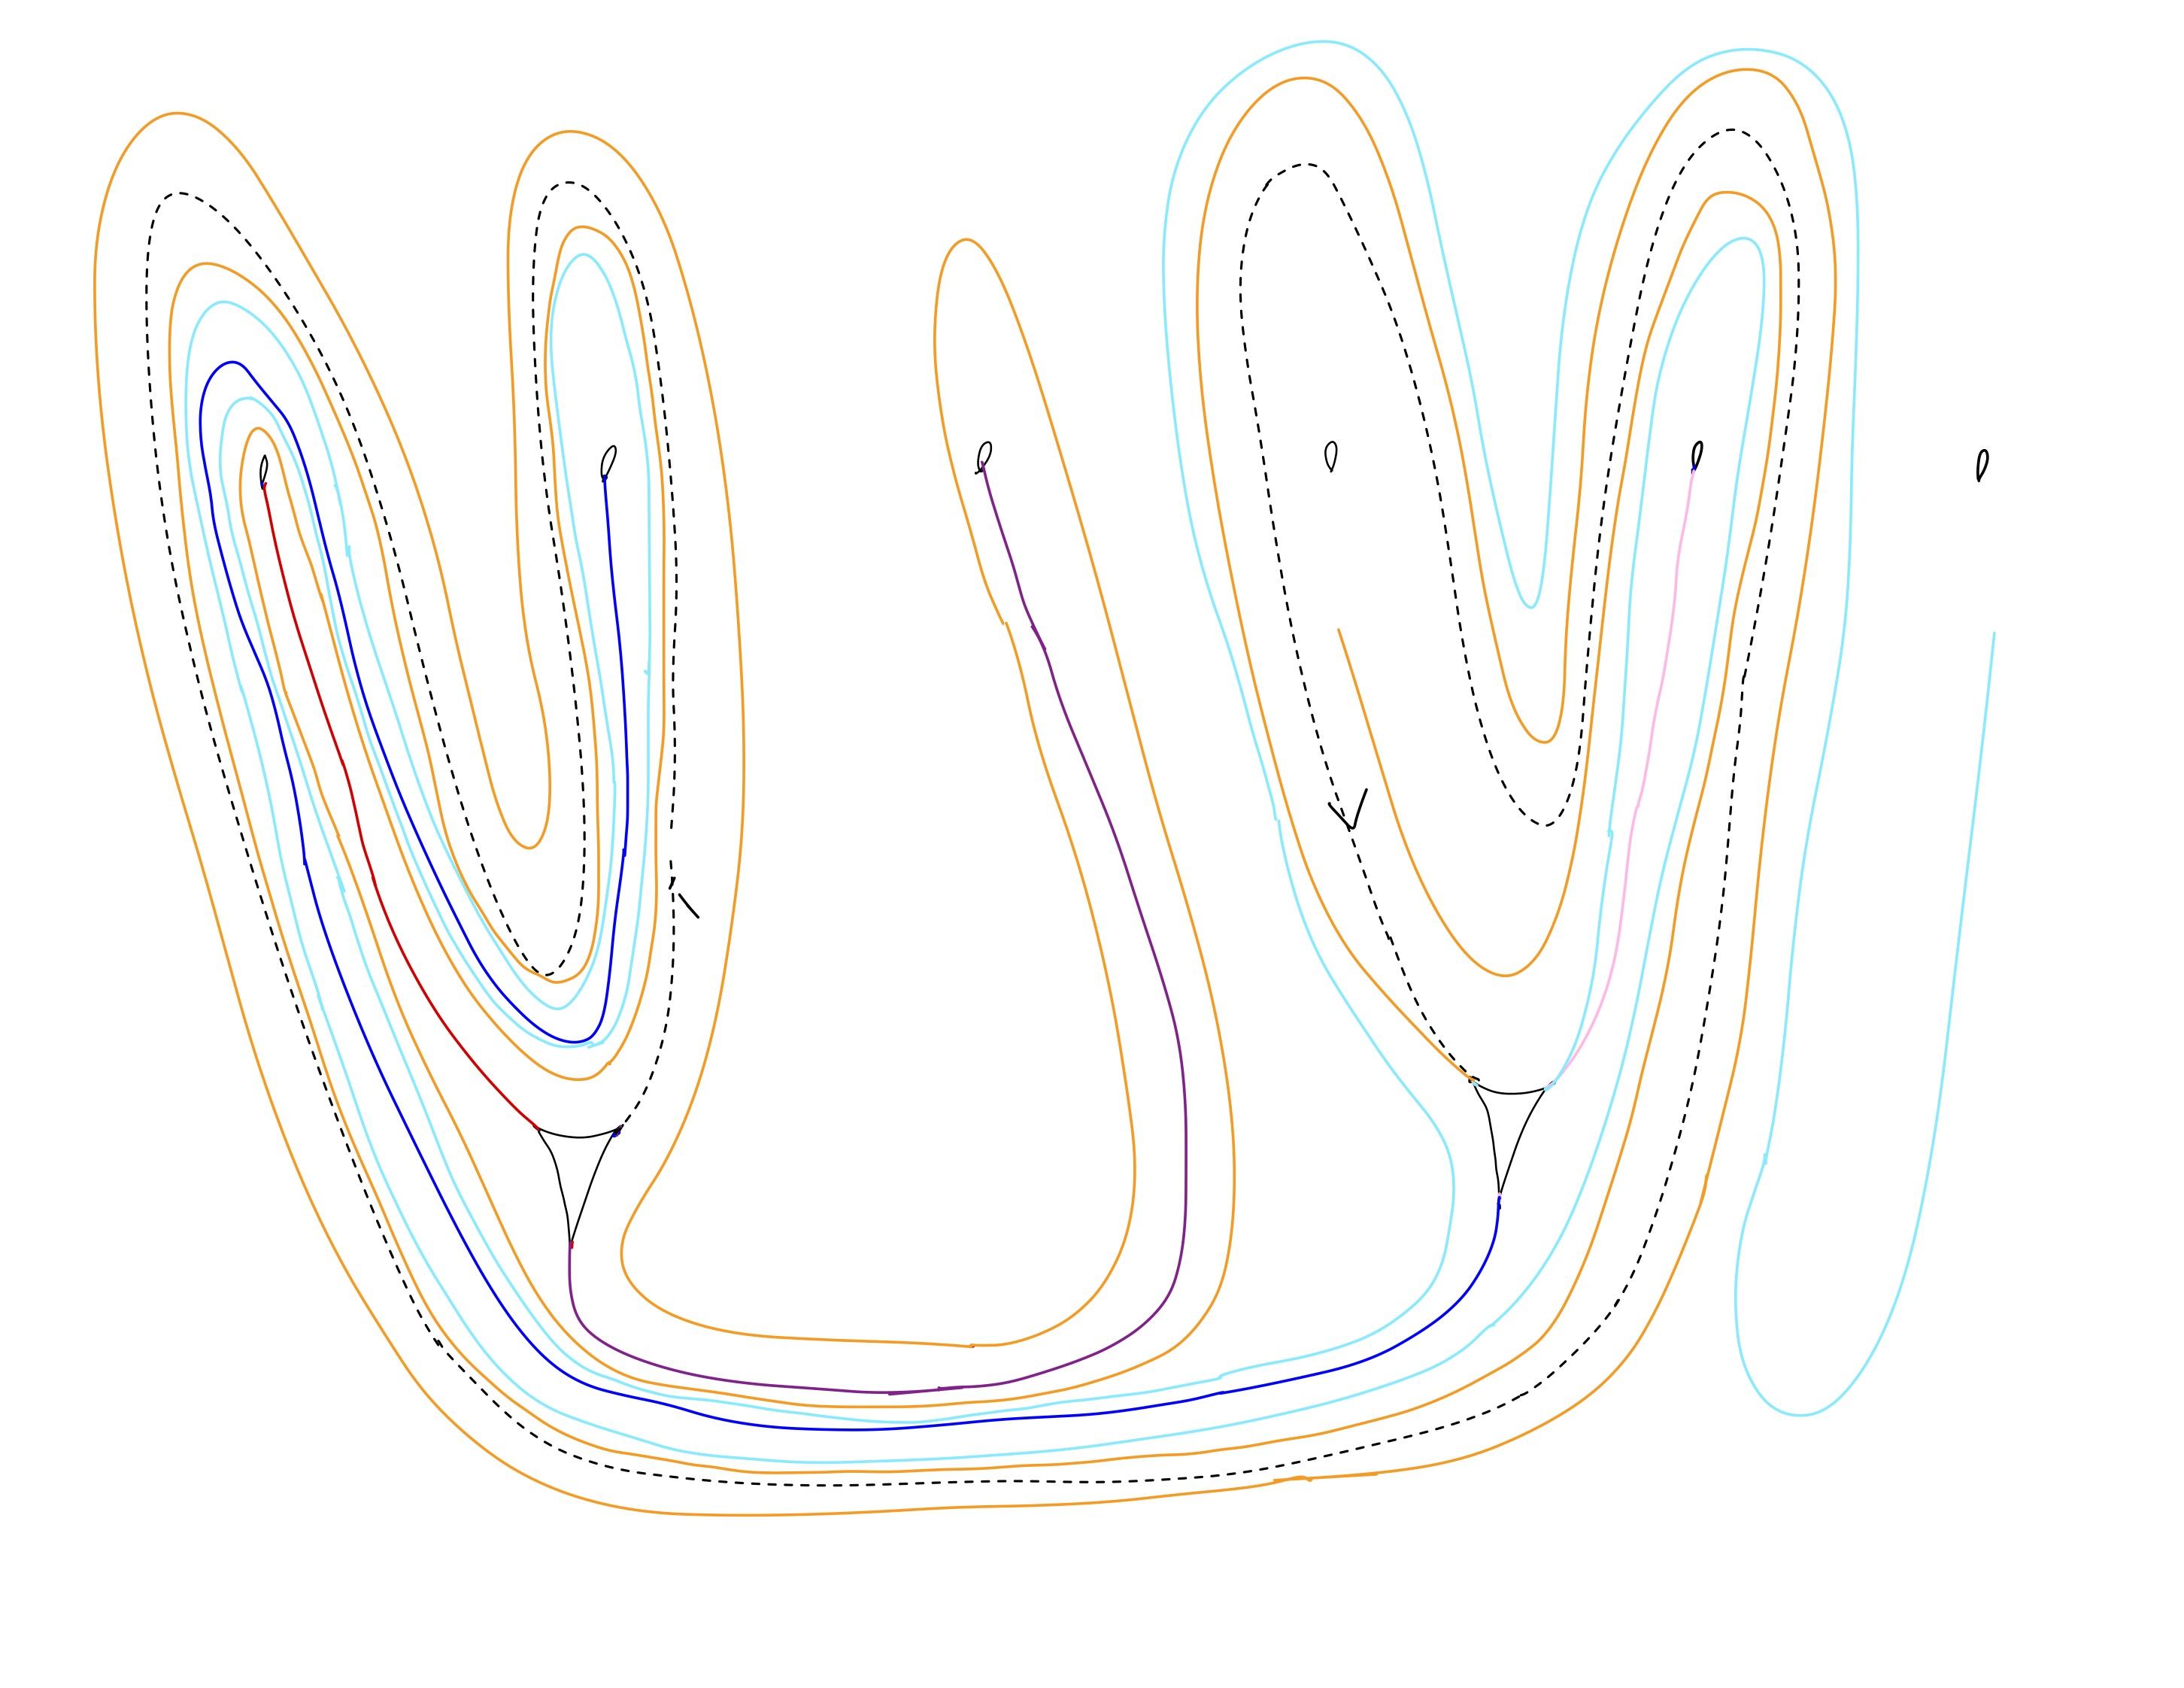
\includegraphics[width=\linewidth]{figures_case_analysis/track17_case_analysis/Roop-05.jpg}
    \caption{Roop5}
    \label{fig:Roop5}
\end{figure}

\begin{figure}[ht]
    \centering
    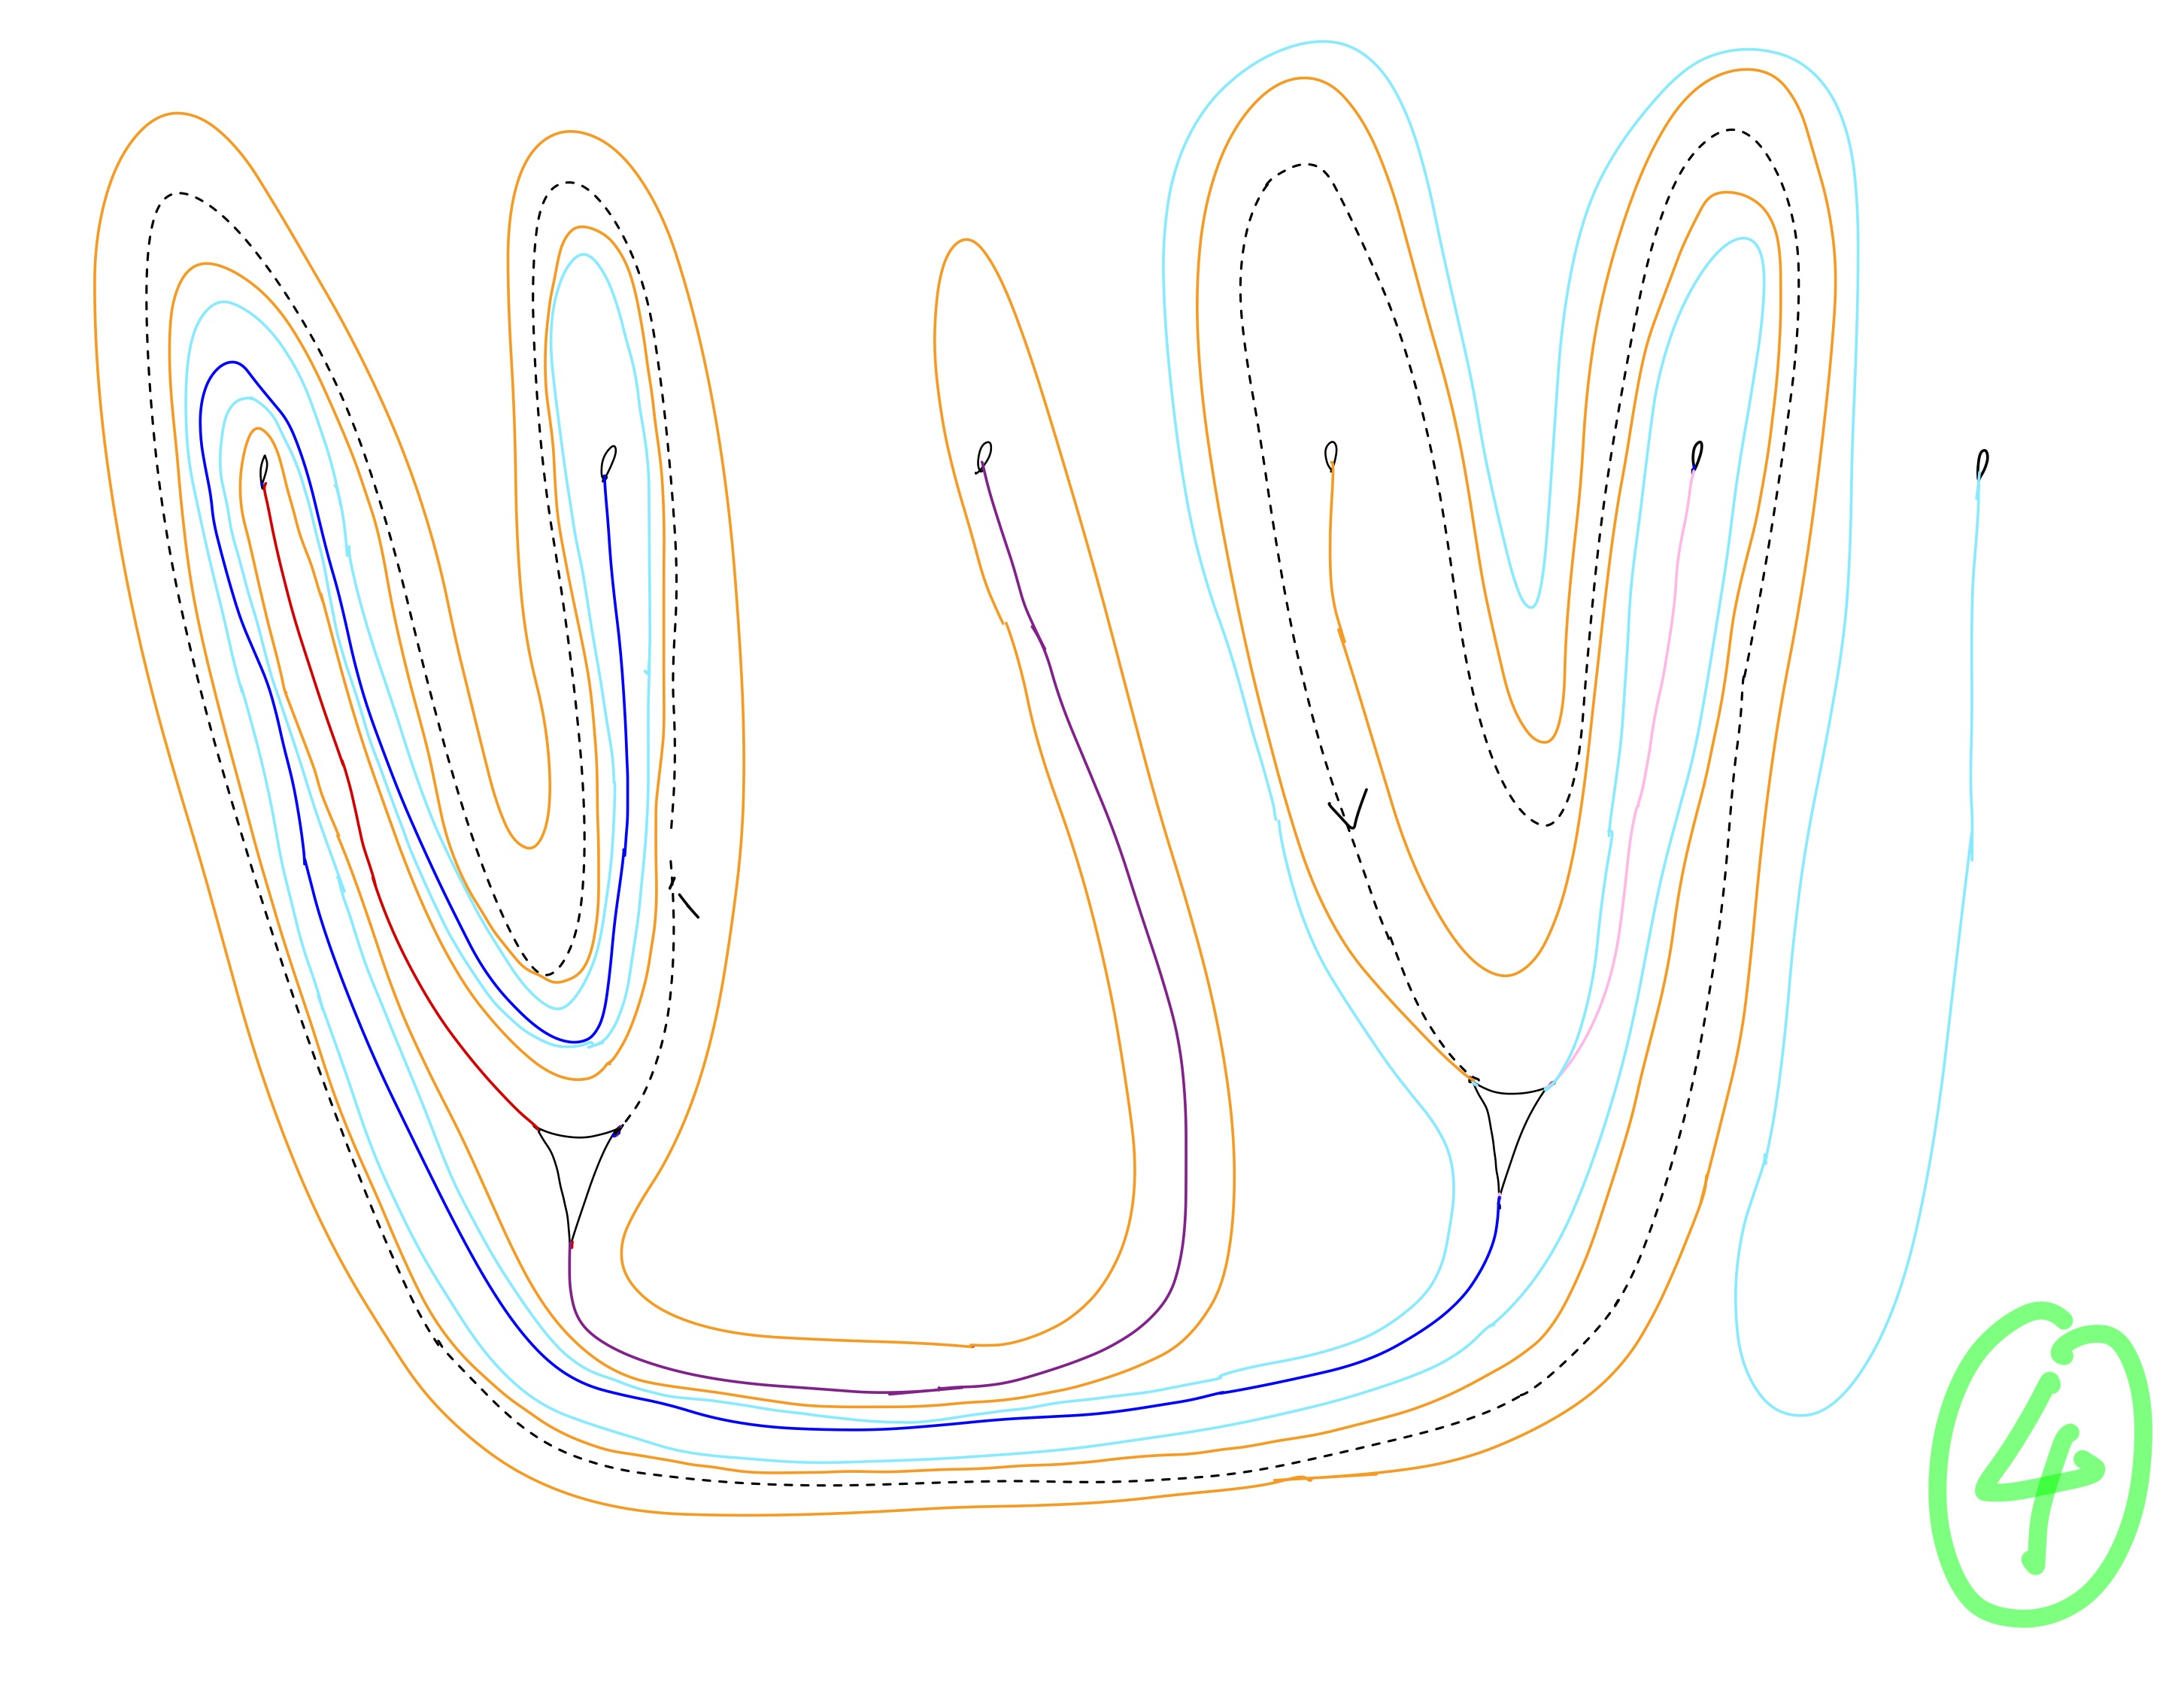
\includegraphics[width=\linewidth]{figures_case_analysis/track17_case_analysis/Roop-06.jpg}
    \caption{Roop6}
    \label{fig:Roop6}
\end{figure}

\begin{figure}[ht]
    \centering
    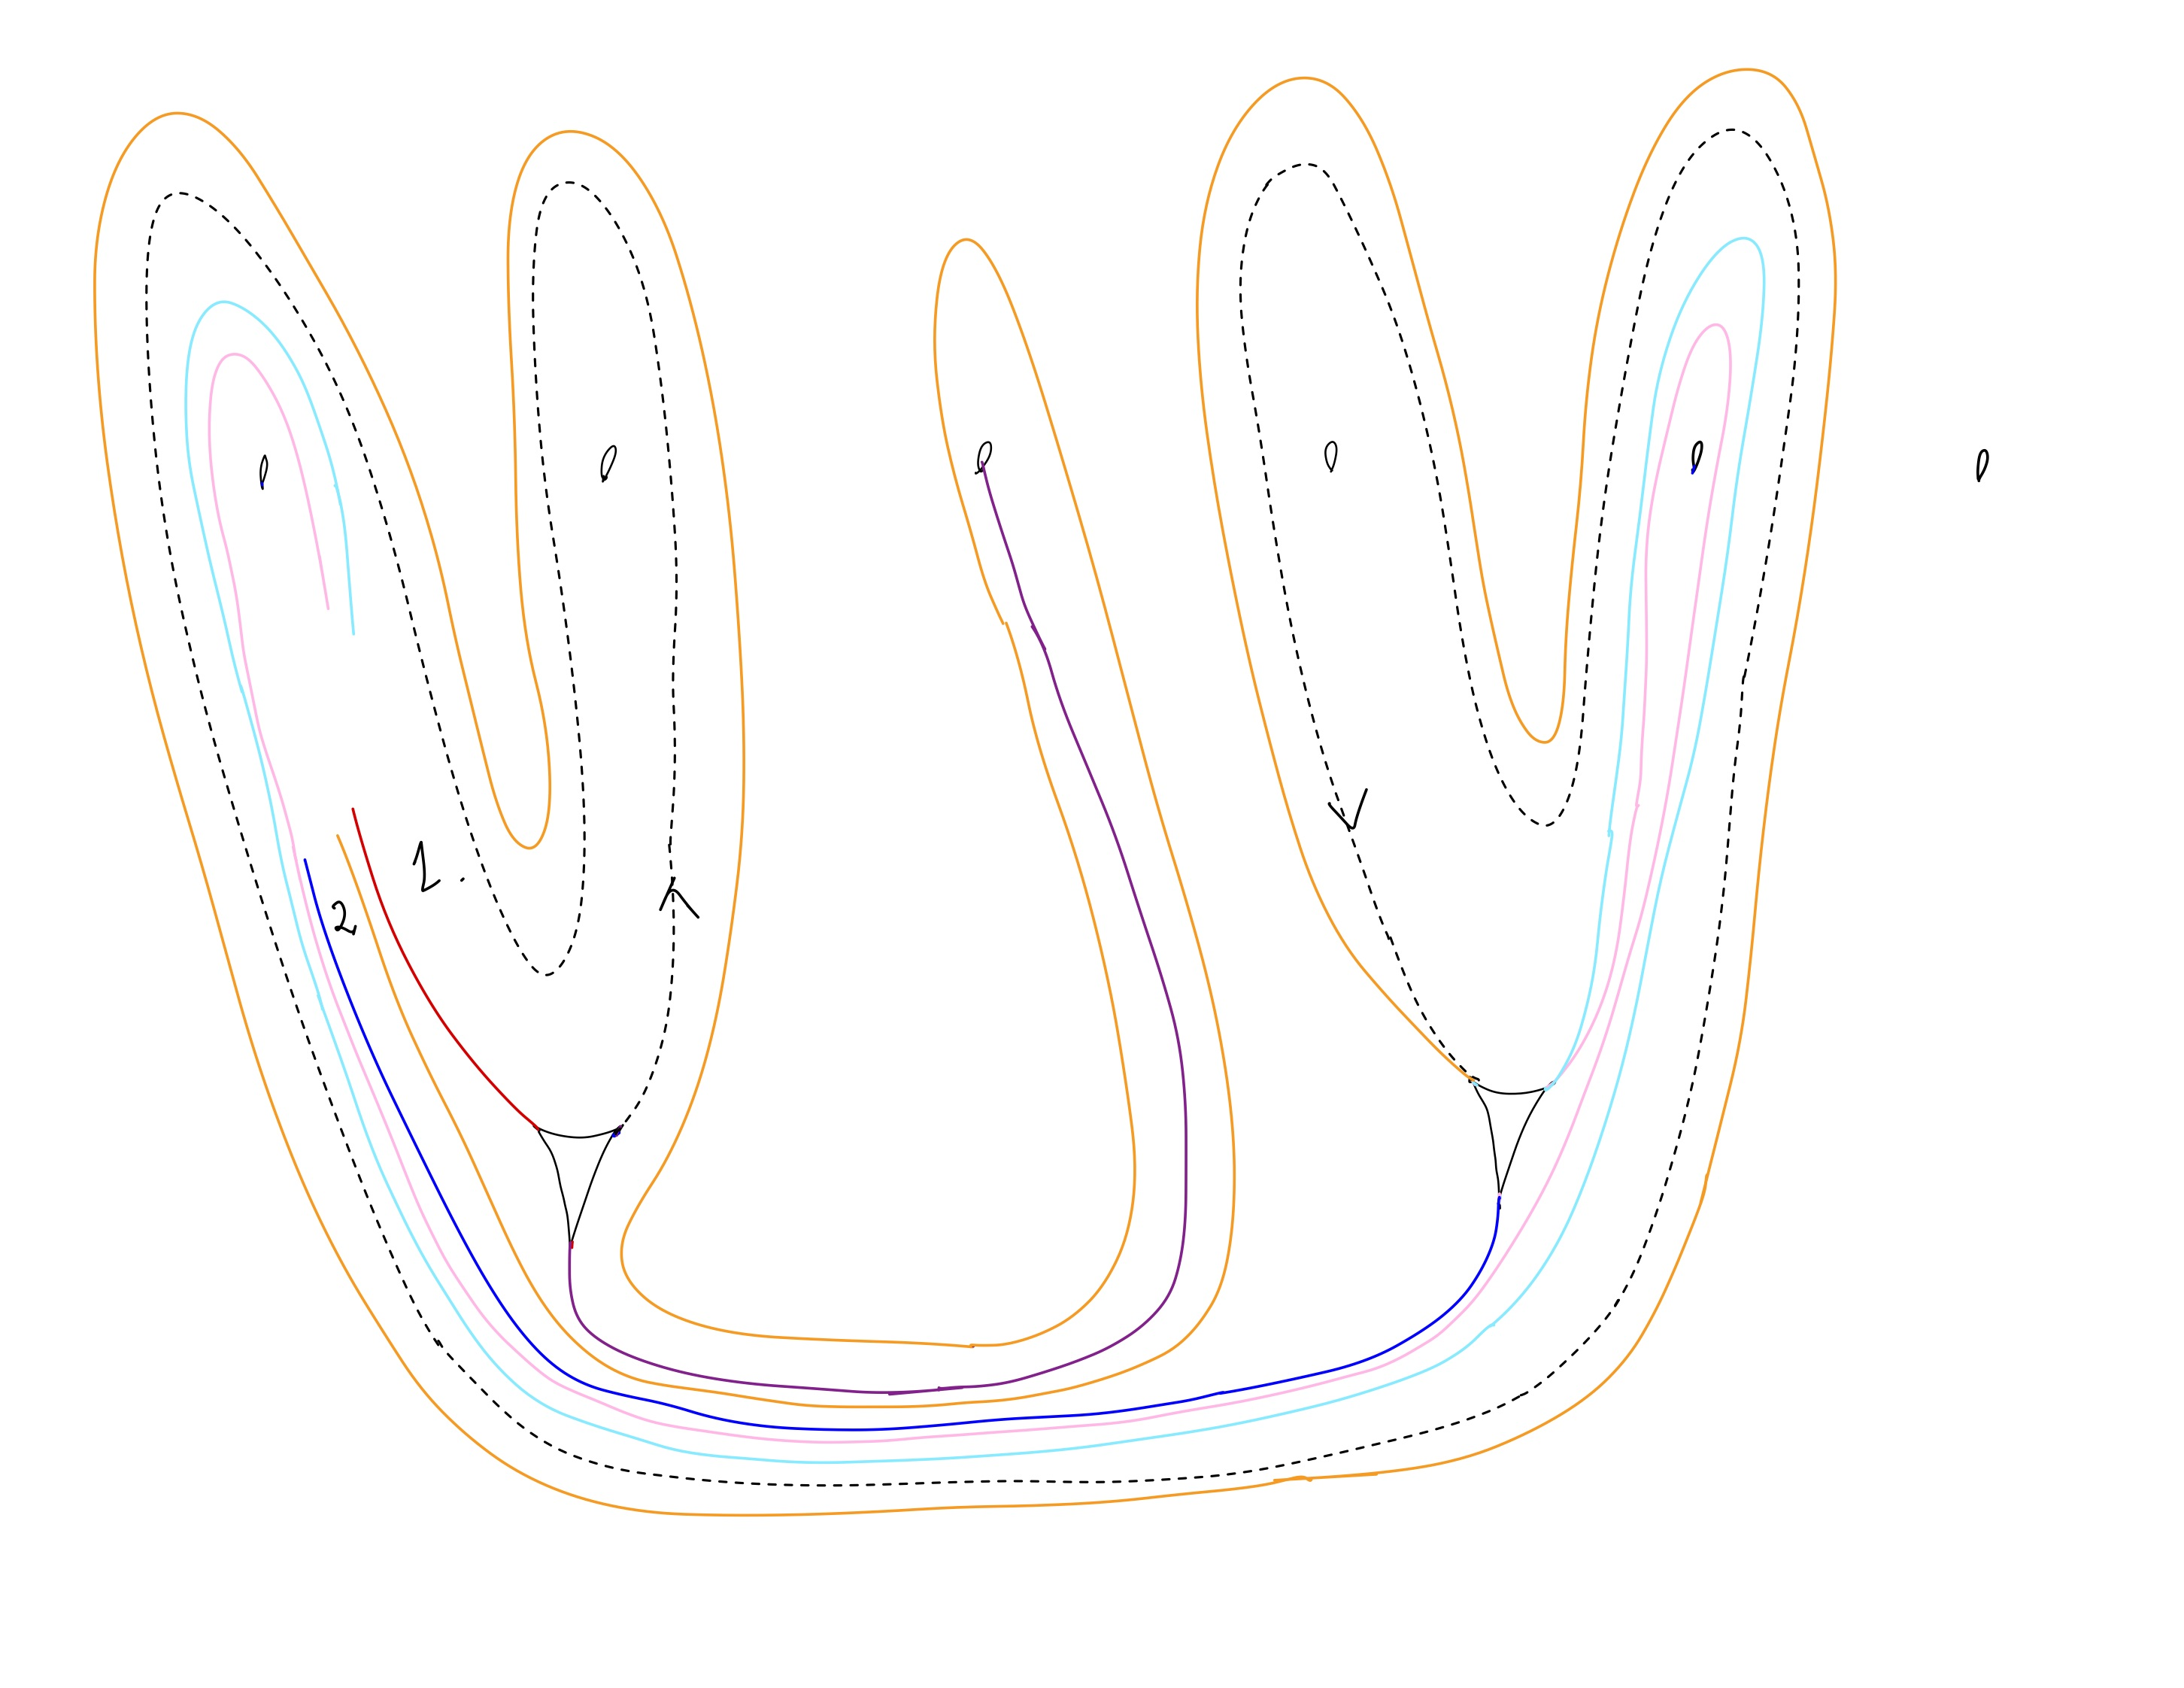
\includegraphics[width=\linewidth]{figures_case_analysis/track17_case_analysis/Roop-07.jpg}
    \caption{Roop7}
    \label{fig:Roop7}
\end{figure}

\begin{figure}[ht]
    \centering
    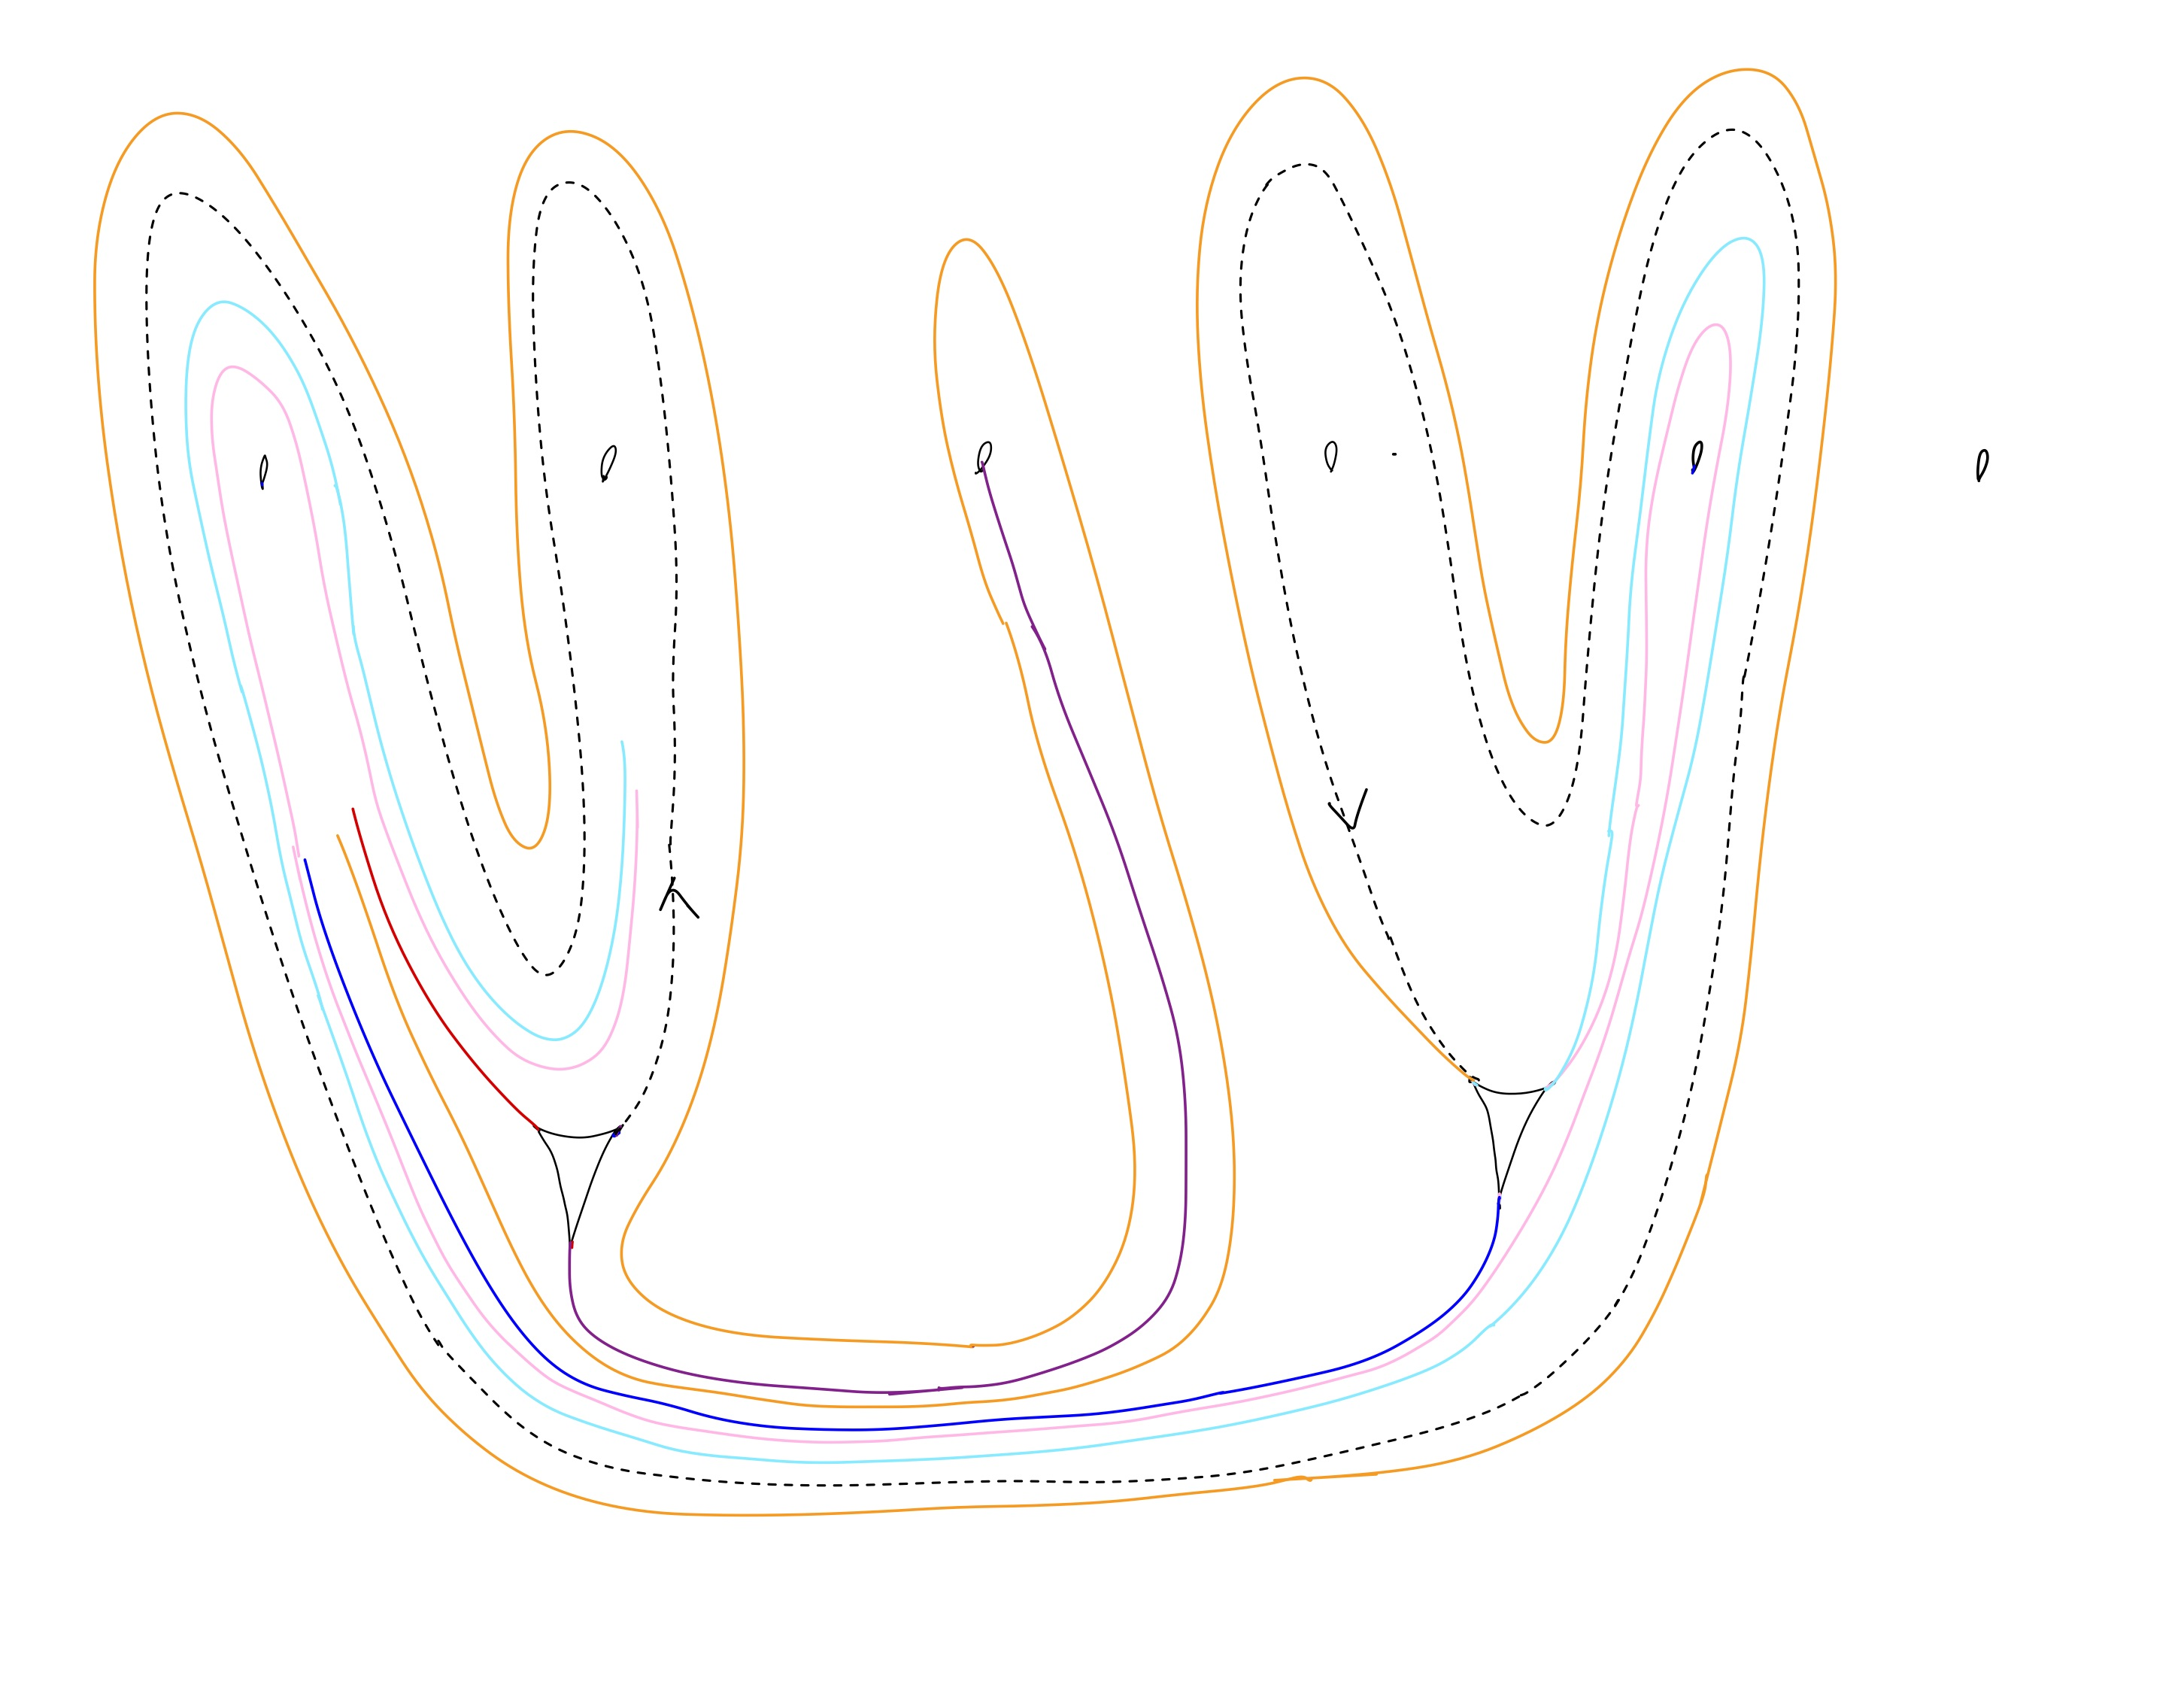
\includegraphics[width=\linewidth]{figures_case_analysis/track17_case_analysis/Roop-08.jpg}
    \caption{Roop8}
    \label{fig:Roop8}
\end{figure}

\begin{figure}[ht]
    \centering
    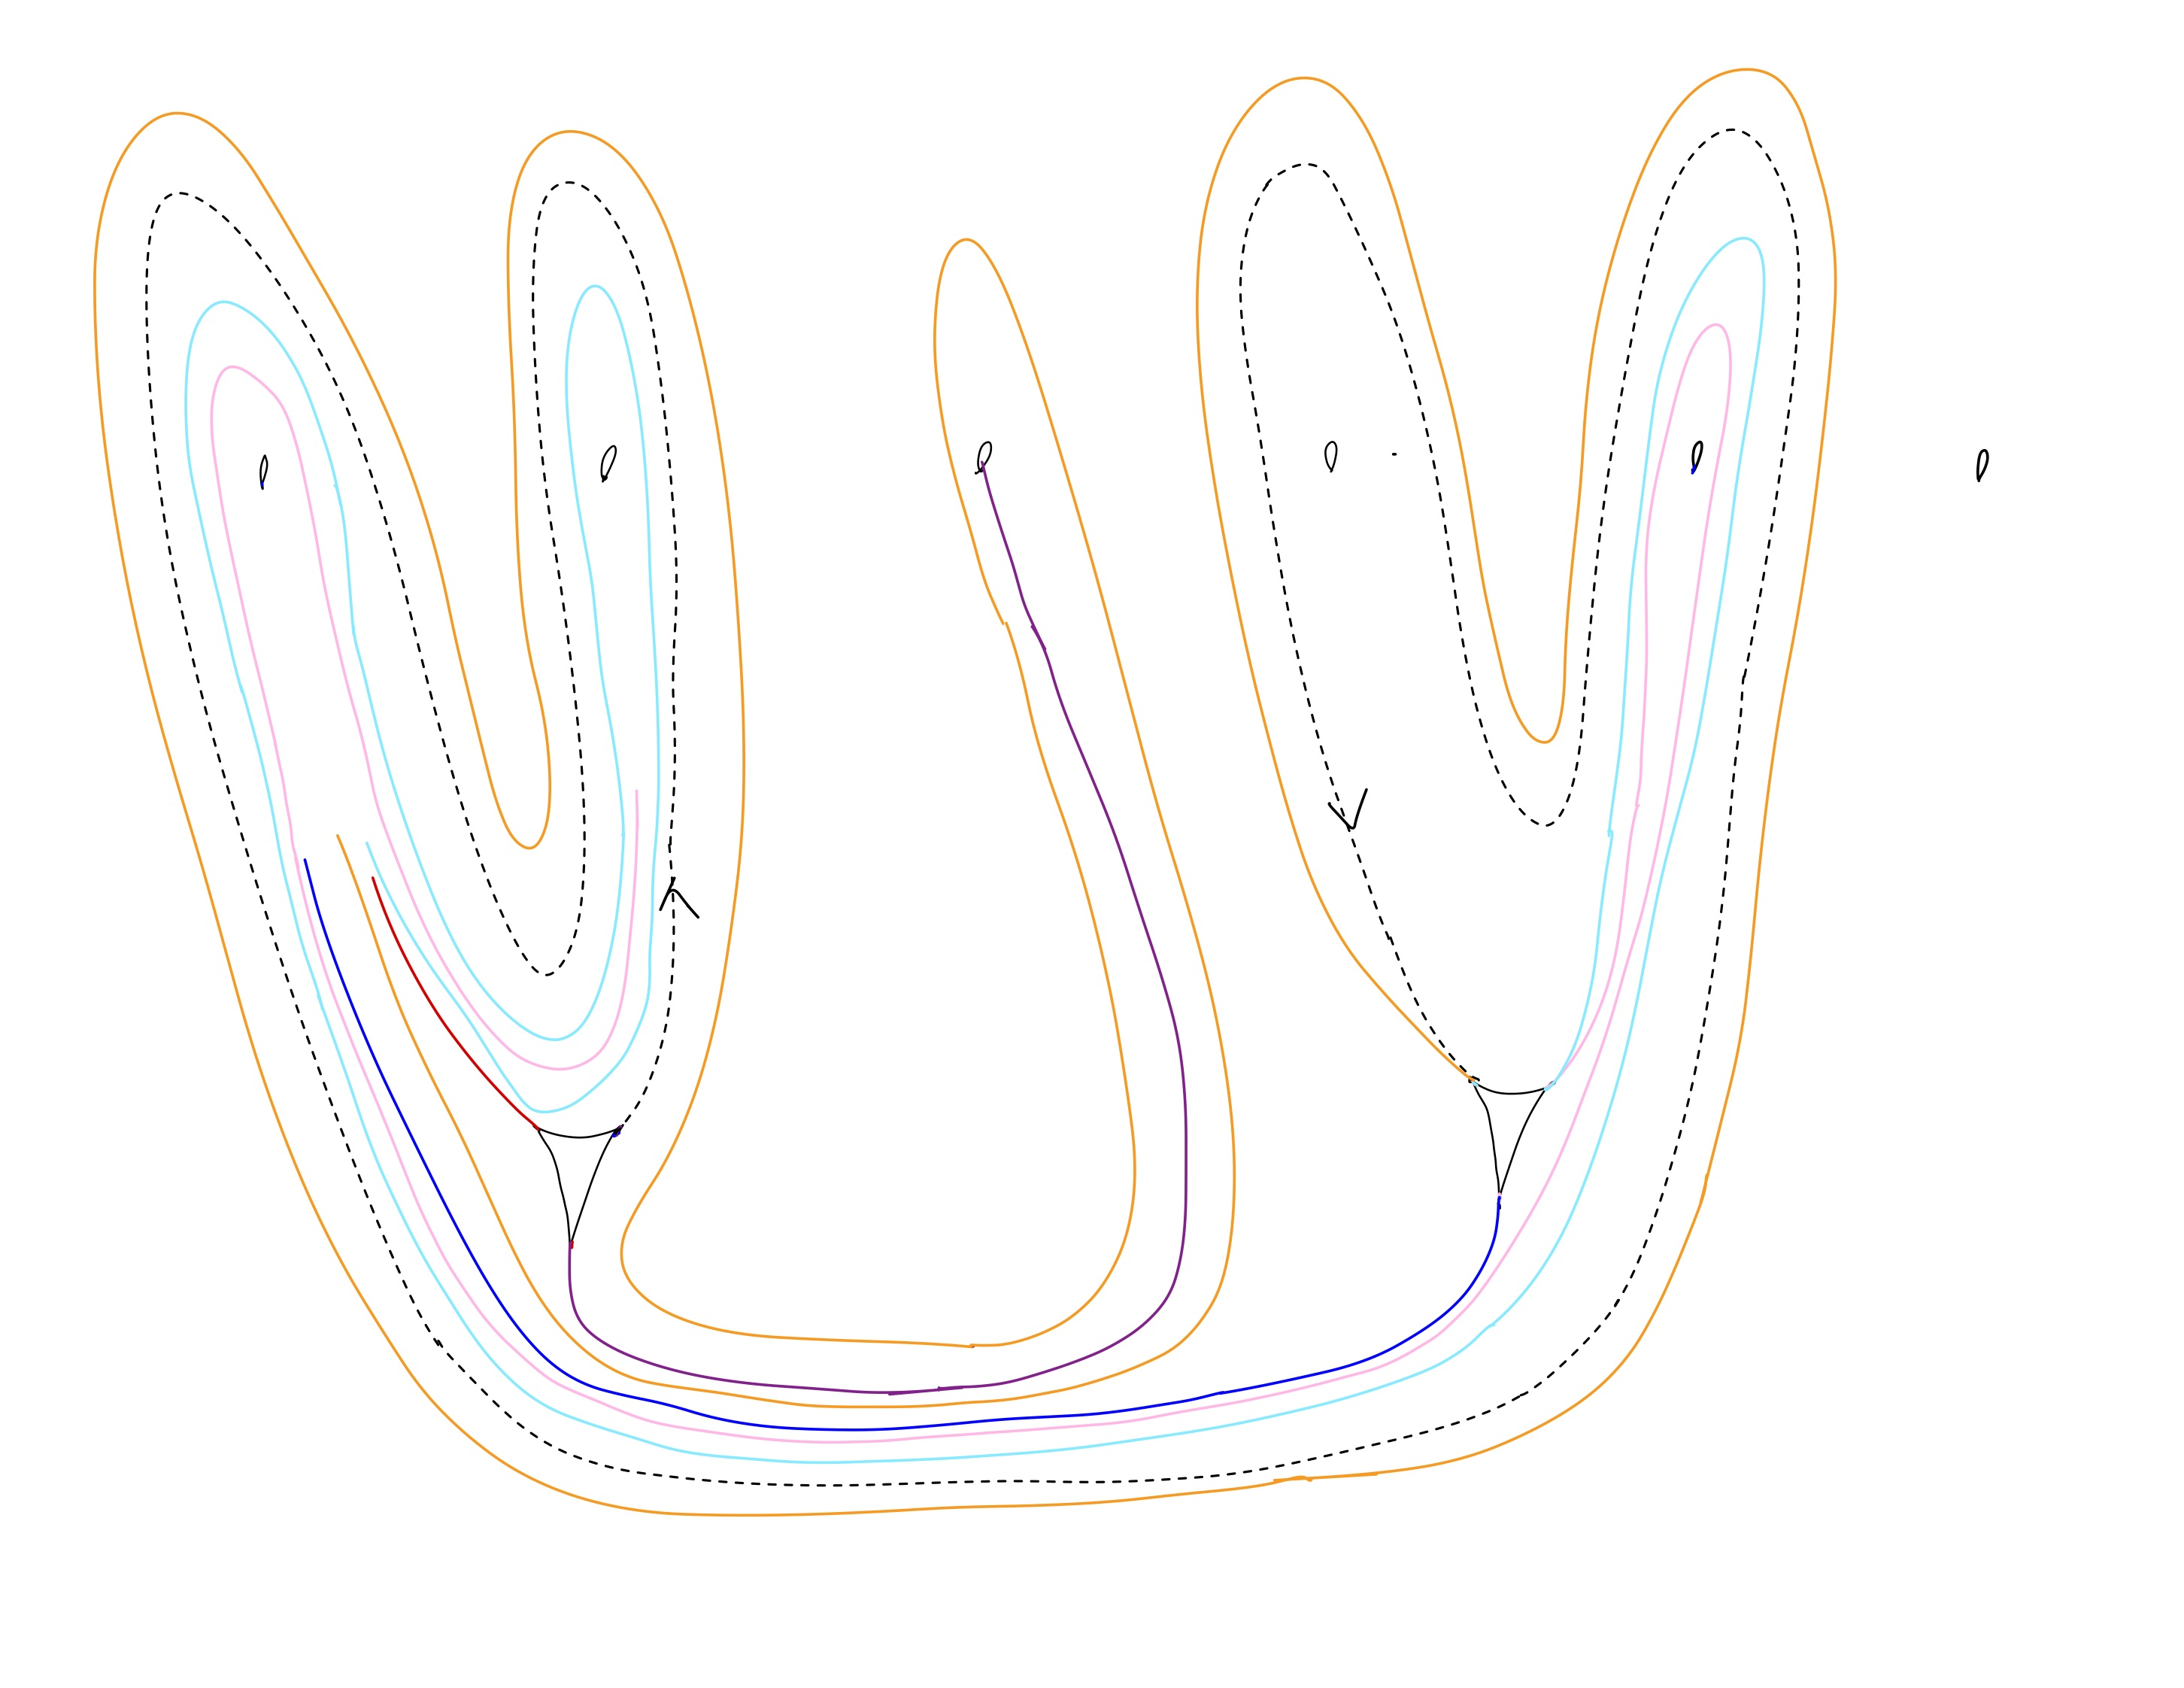
\includegraphics[width=\linewidth]{figures_case_analysis/track17_case_analysis/Roop-09.jpg}
    \caption{Roop9}
    \label{fig:Roop9}
\end{figure}

\begin{figure}[ht]
    \centering
    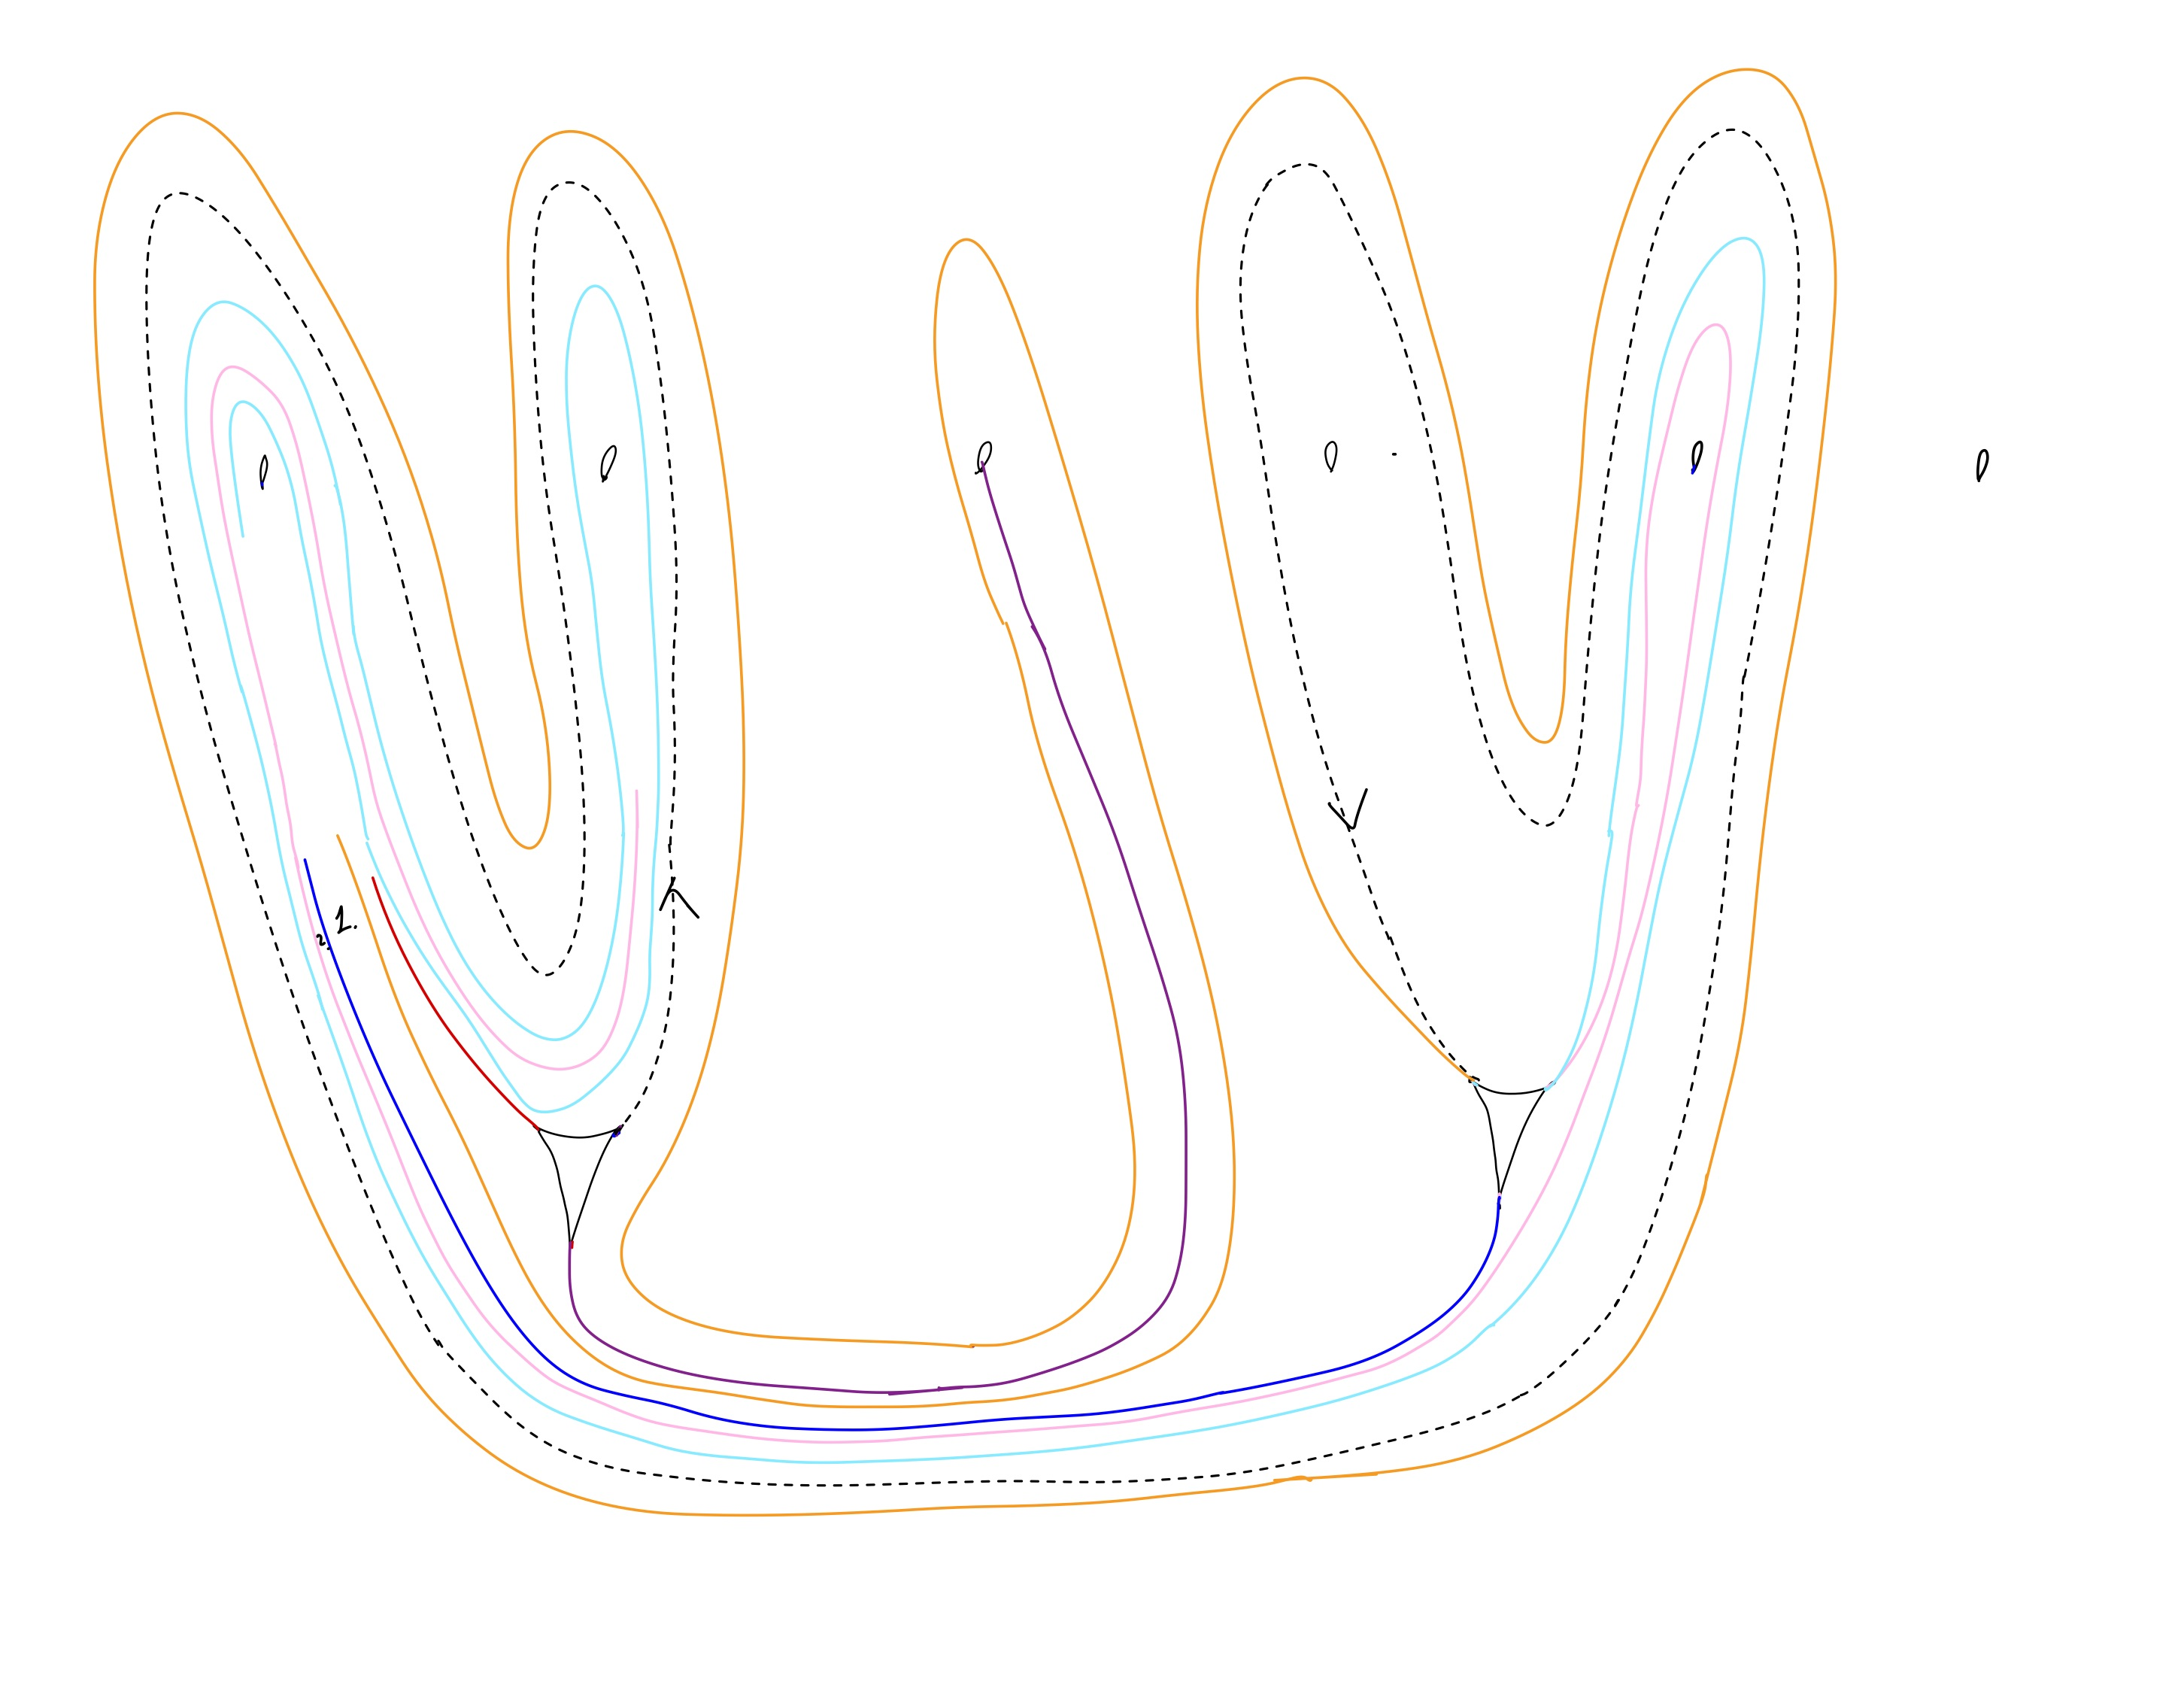
\includegraphics[width=\linewidth]{figures_case_analysis/track17_case_analysis/Roop-10.jpg}
    \caption{Roop10}
    \label{fig:Roop10}
\end{figure}

\begin{figure}[ht]
    \centering
    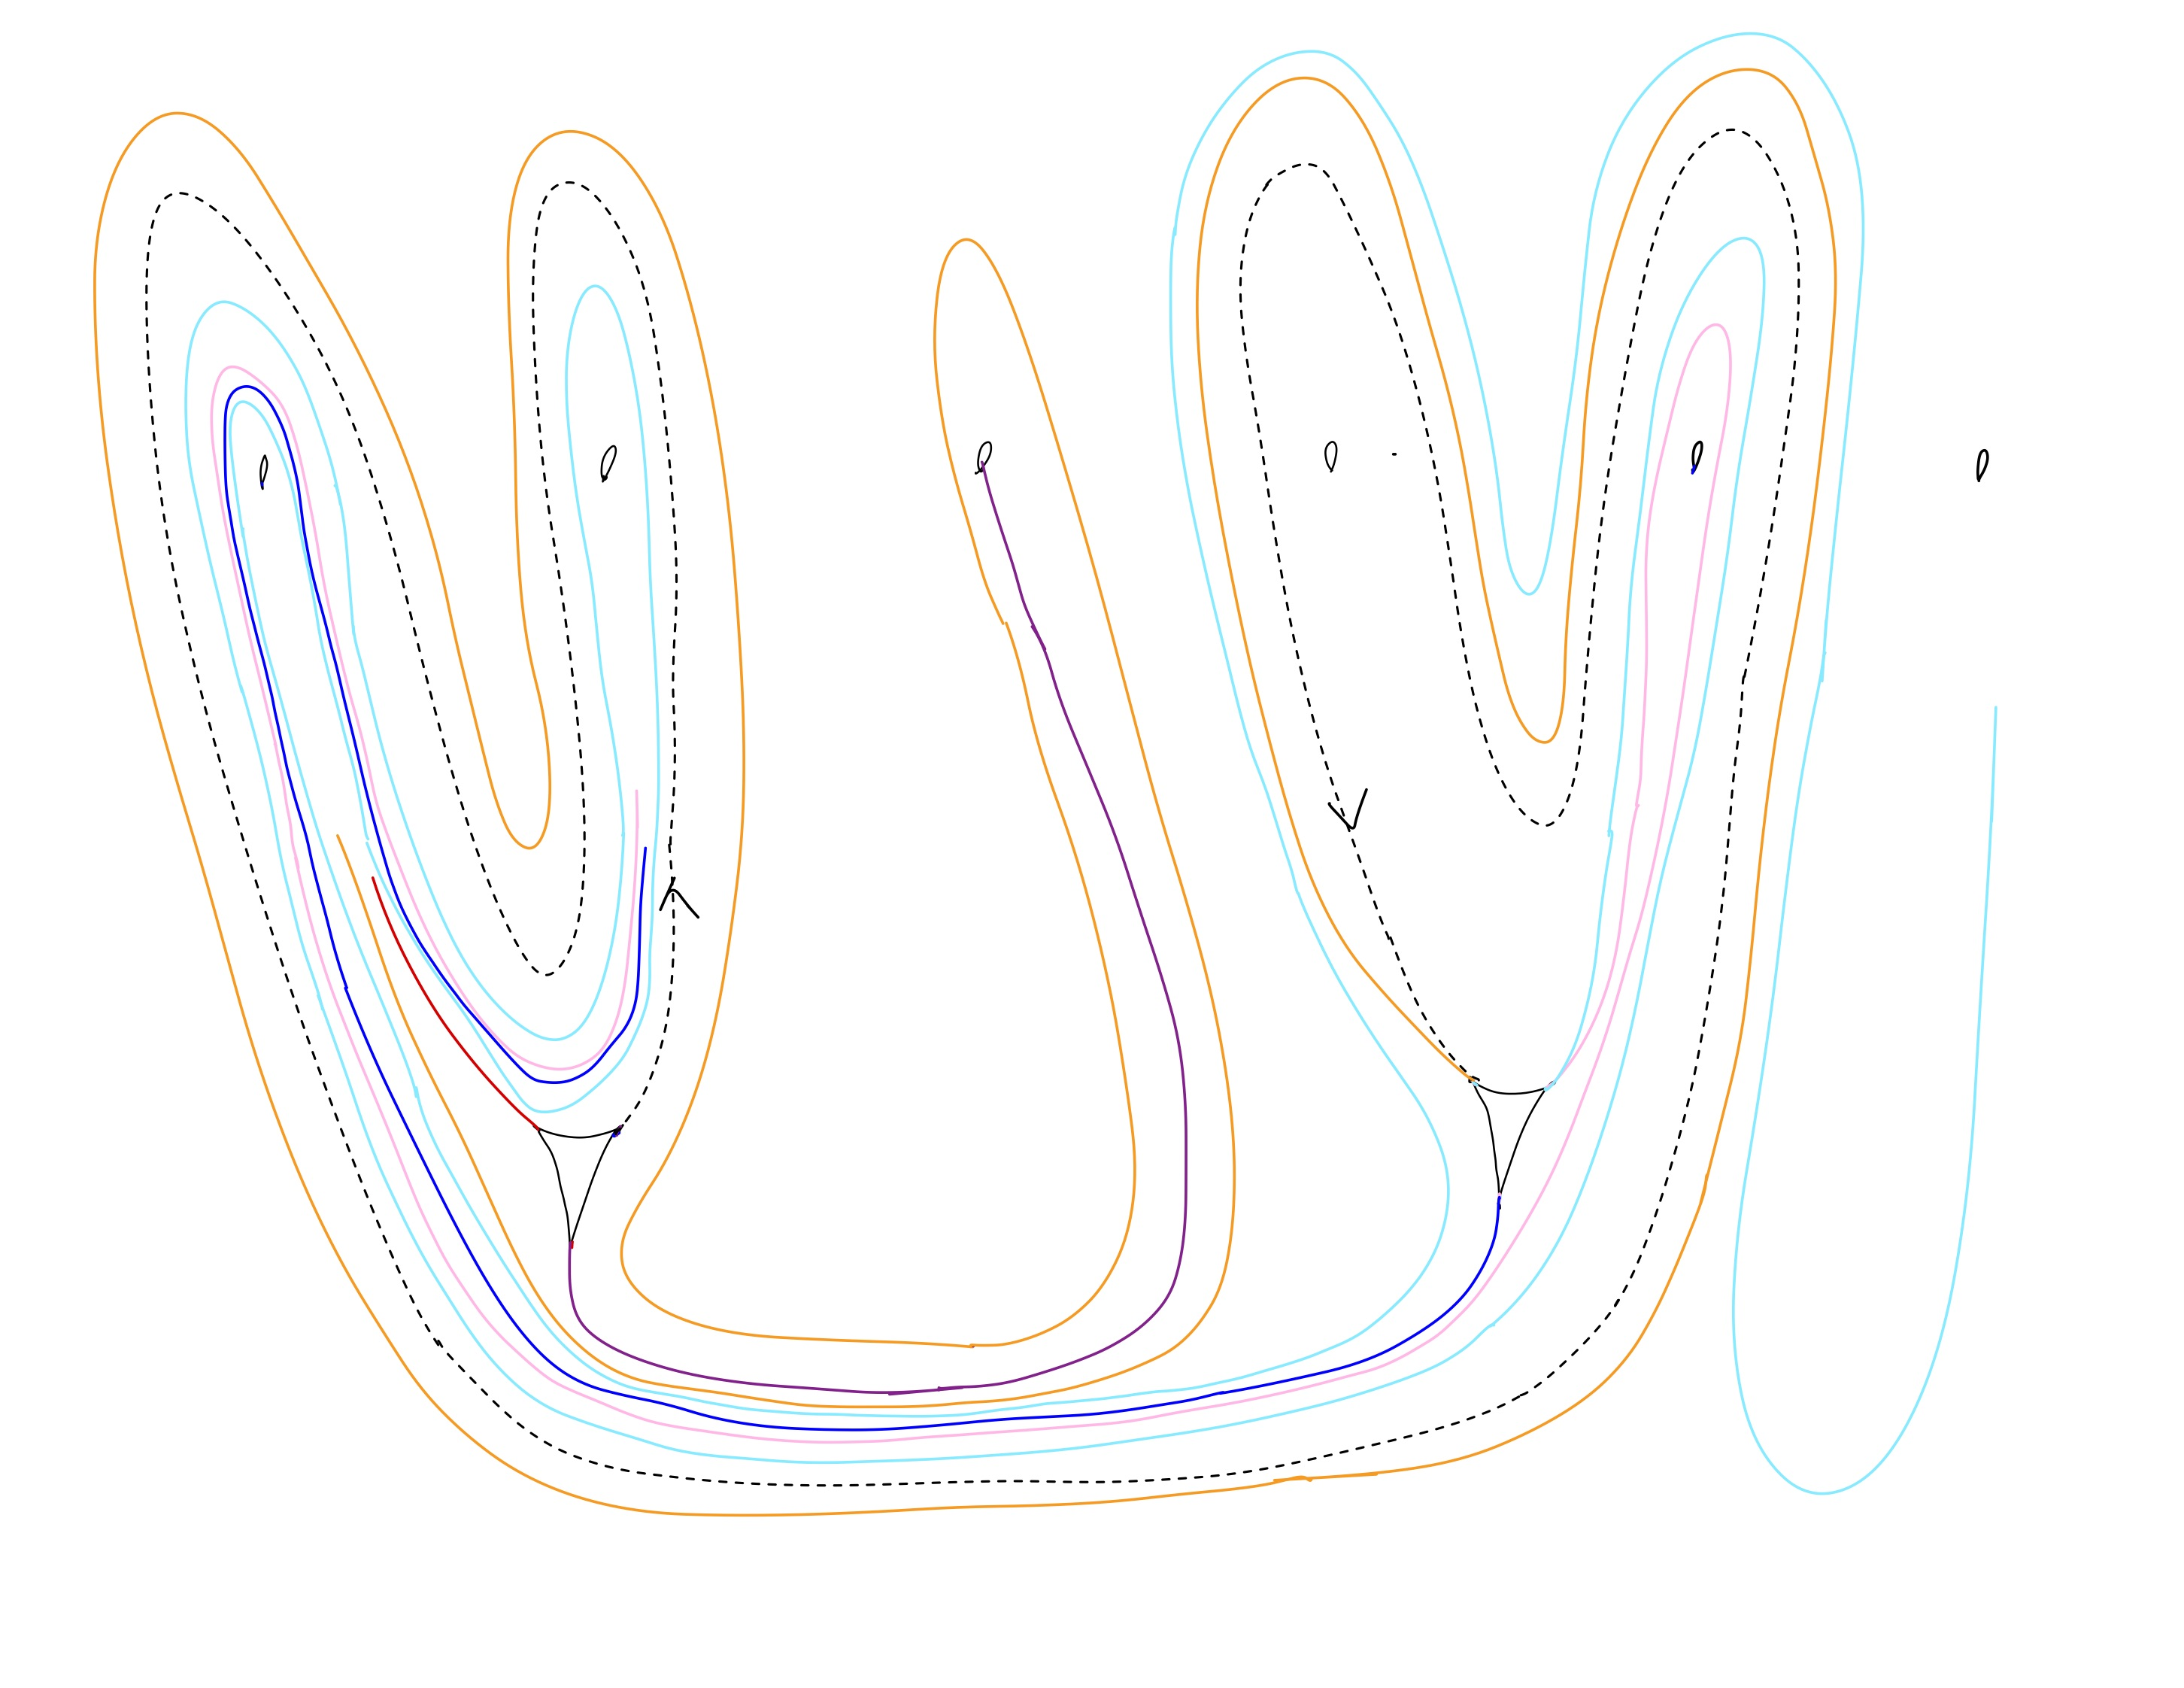
\includegraphics[width=\linewidth]{figures_case_analysis/track17_case_analysis/Roop-11.jpg}
    \caption{Roop11}
    \label{fig:Roop11}
\end{figure}

\begin{figure}[ht]
    \centering
    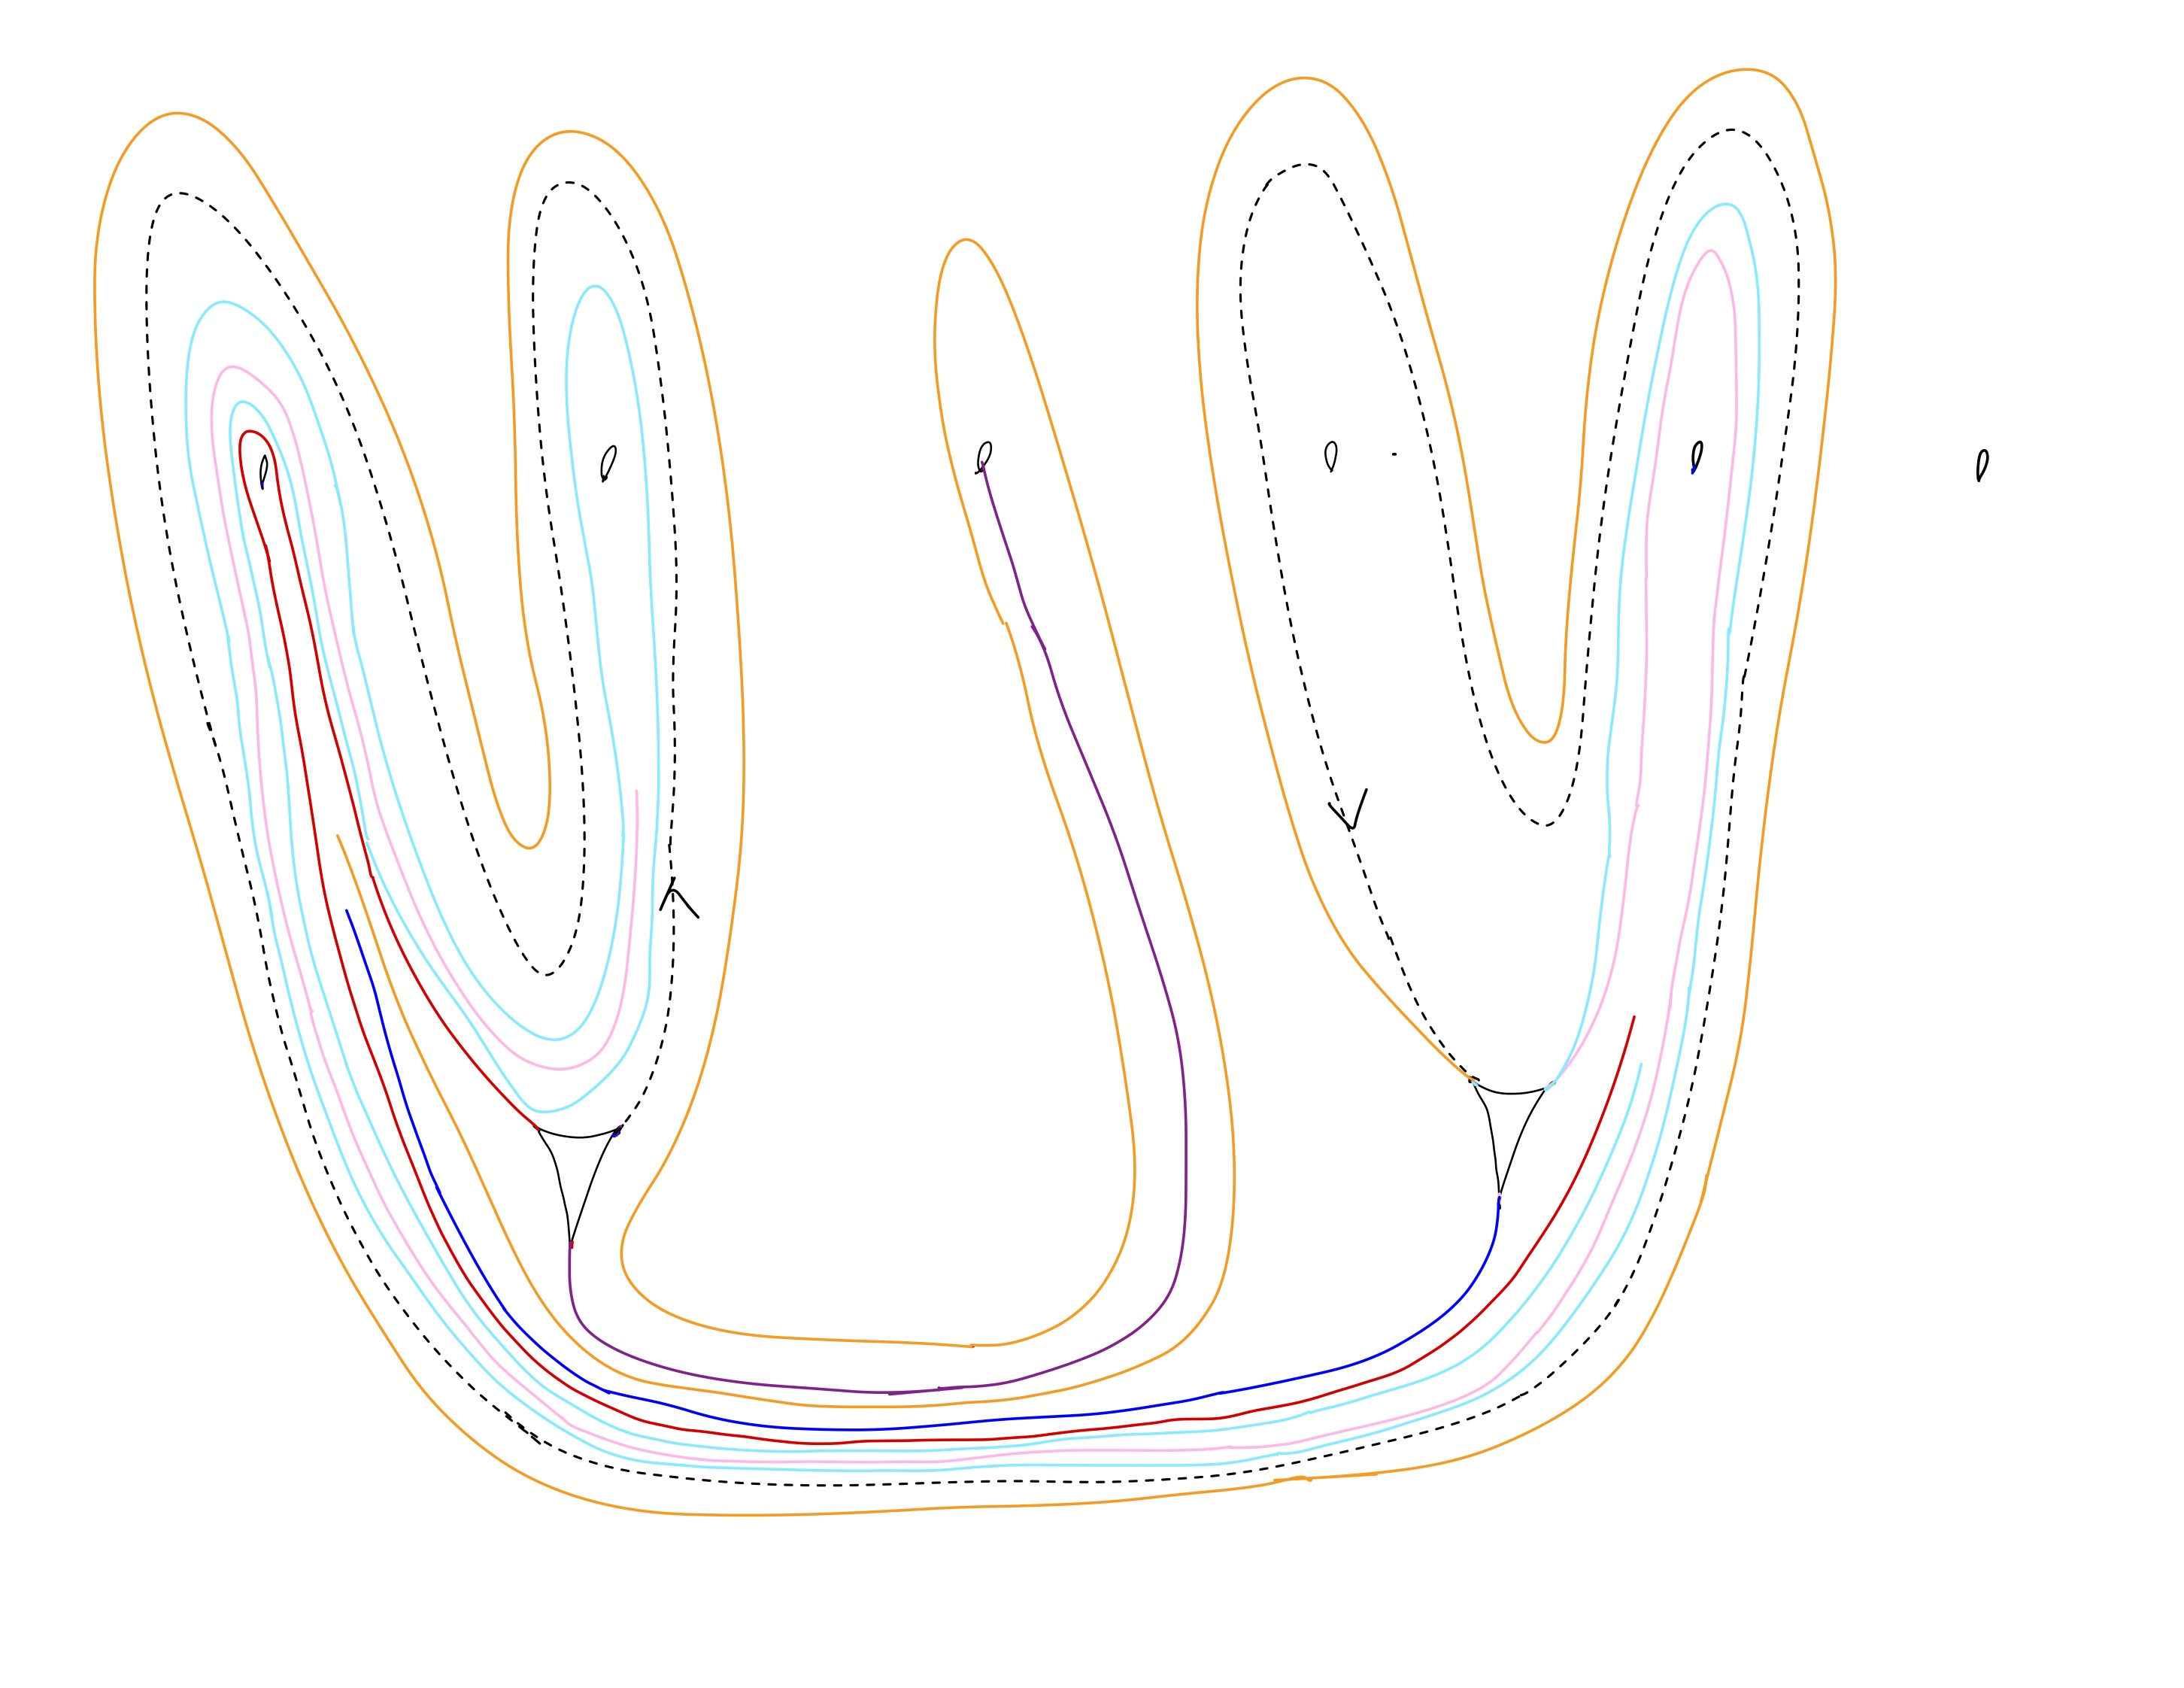
\includegraphics[width=\linewidth]{figures_case_analysis/track17_case_analysis/Roop-12.jpg}
    \caption{Roop12}
    \label{fig:Roop12}
\end{figure}

\begin{figure}[ht]
    \centering
    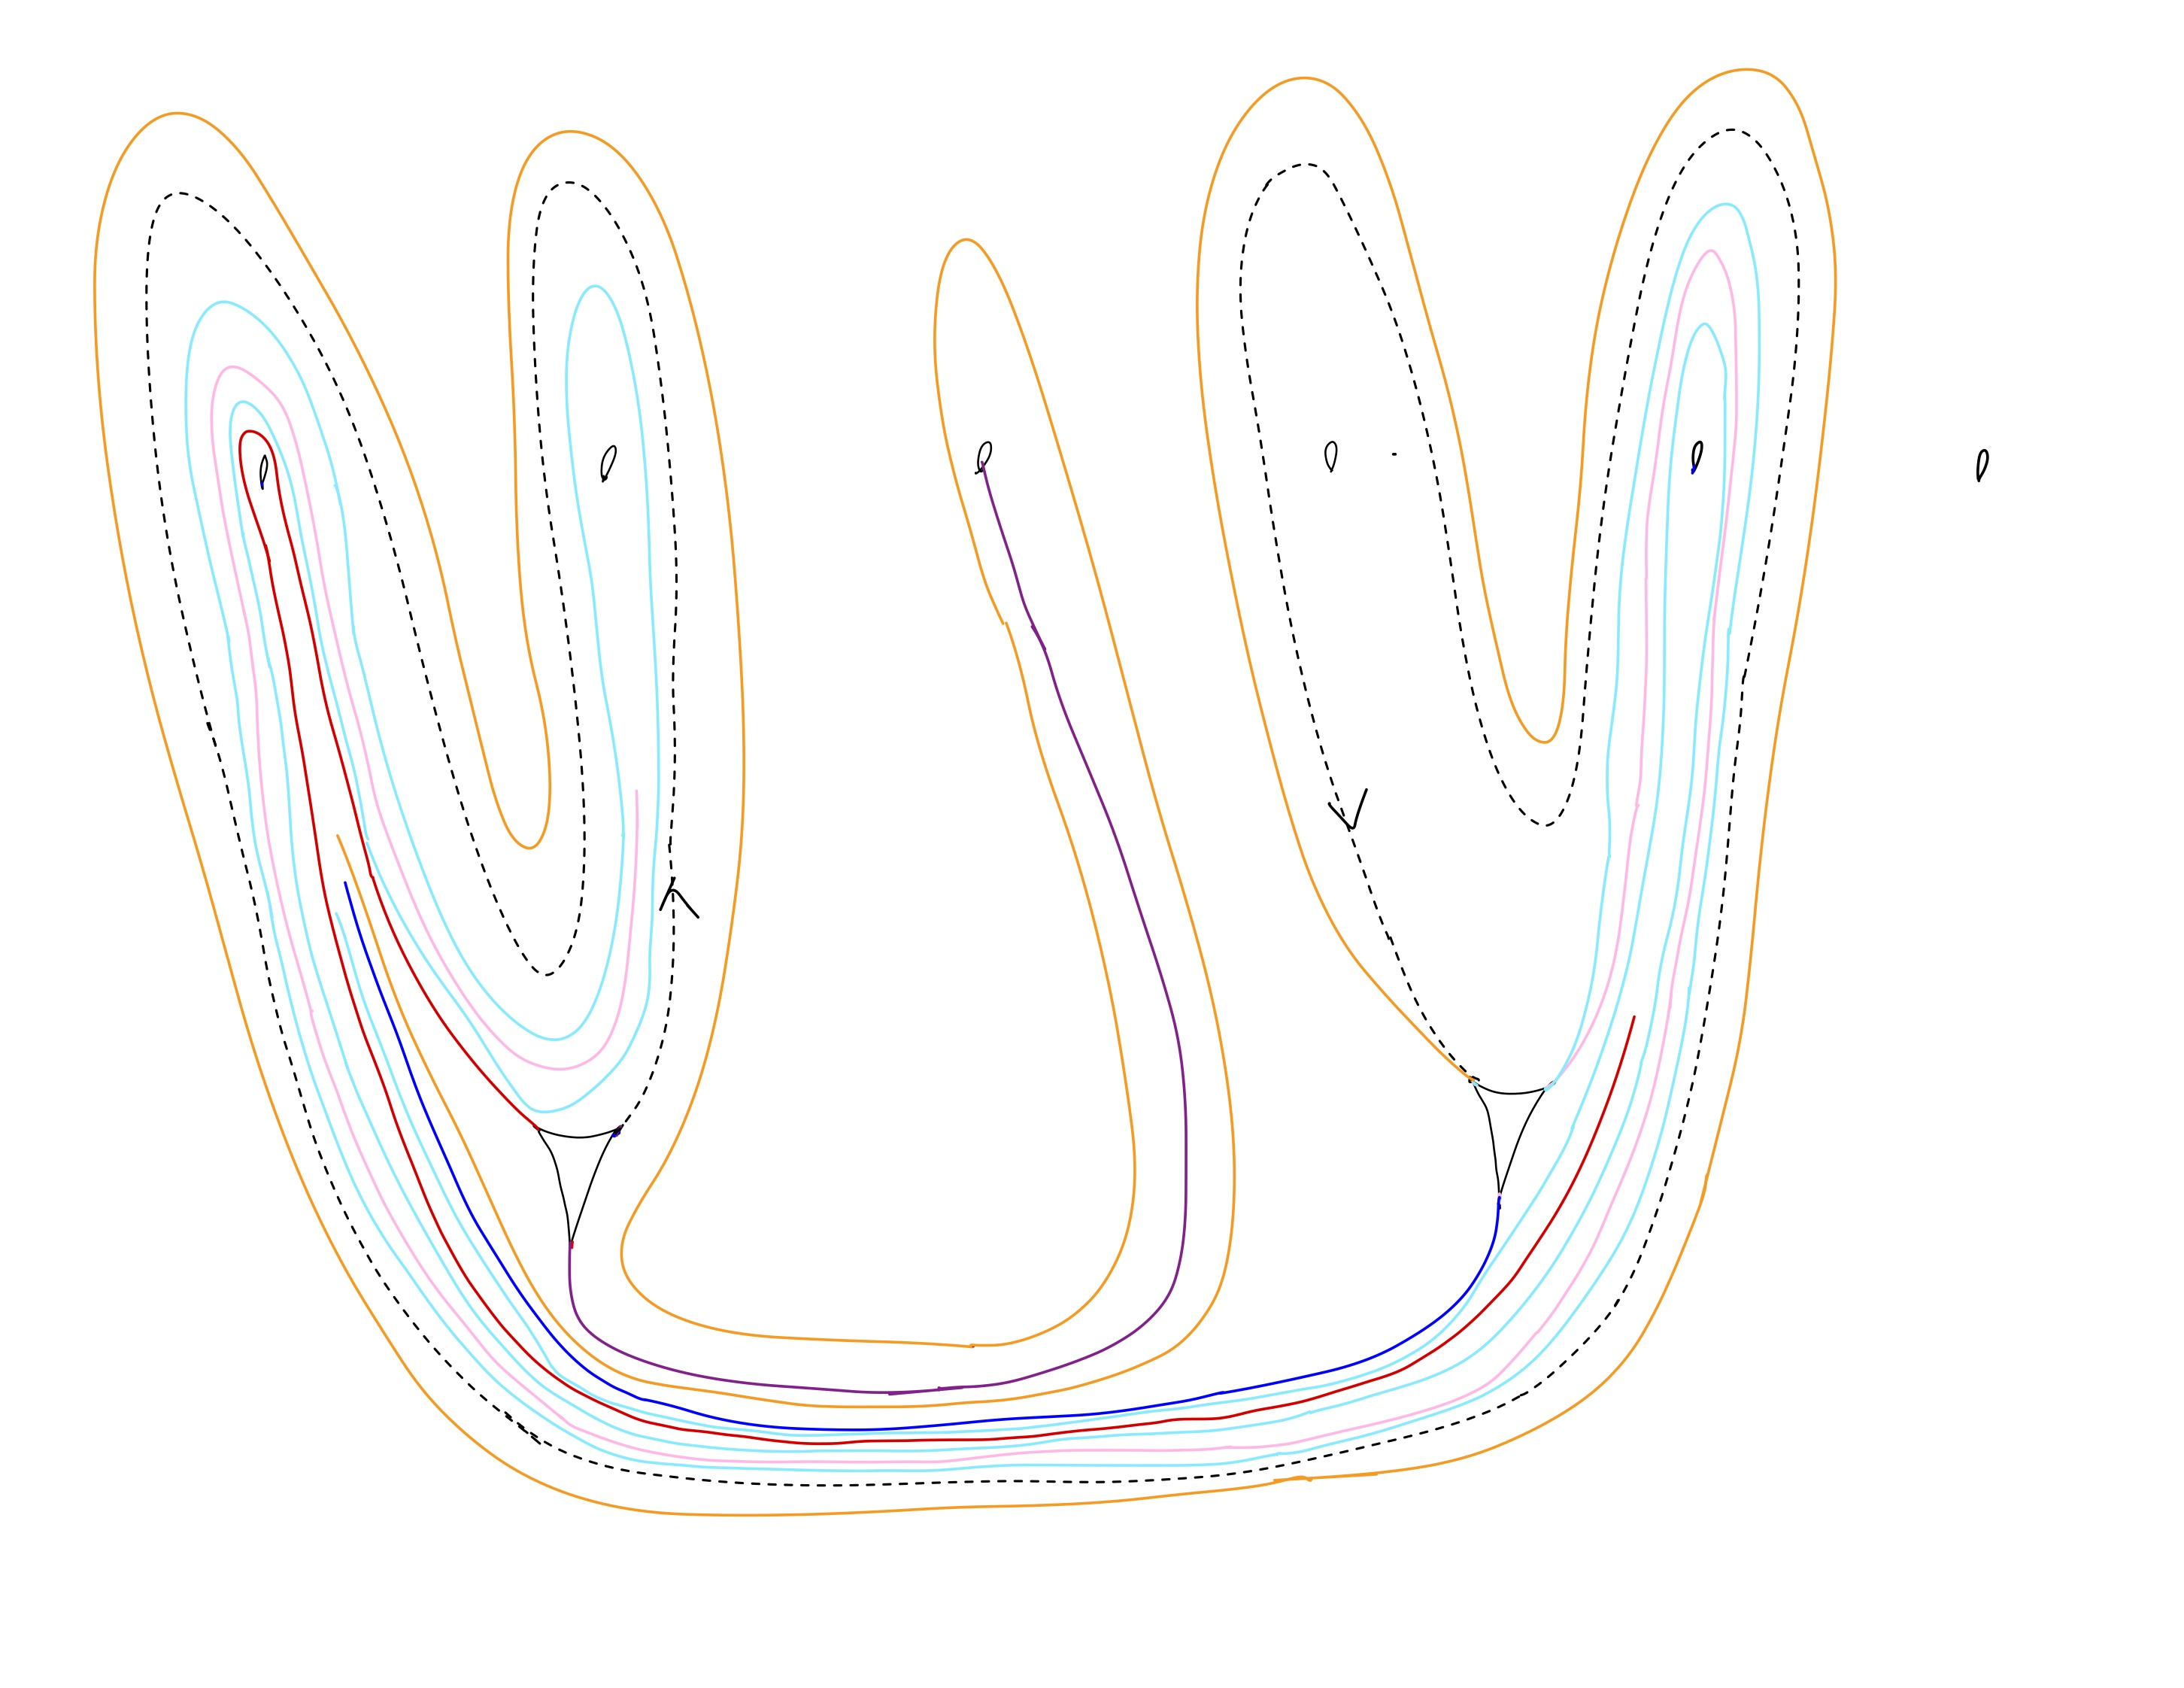
\includegraphics[width=\linewidth]{figures_case_analysis/track17_case_analysis/Roop-13.jpg}
    \caption{Roop13}
    \label{fig:Roop13}
\end{figure}

\begin{figure}[ht]
    \centering
    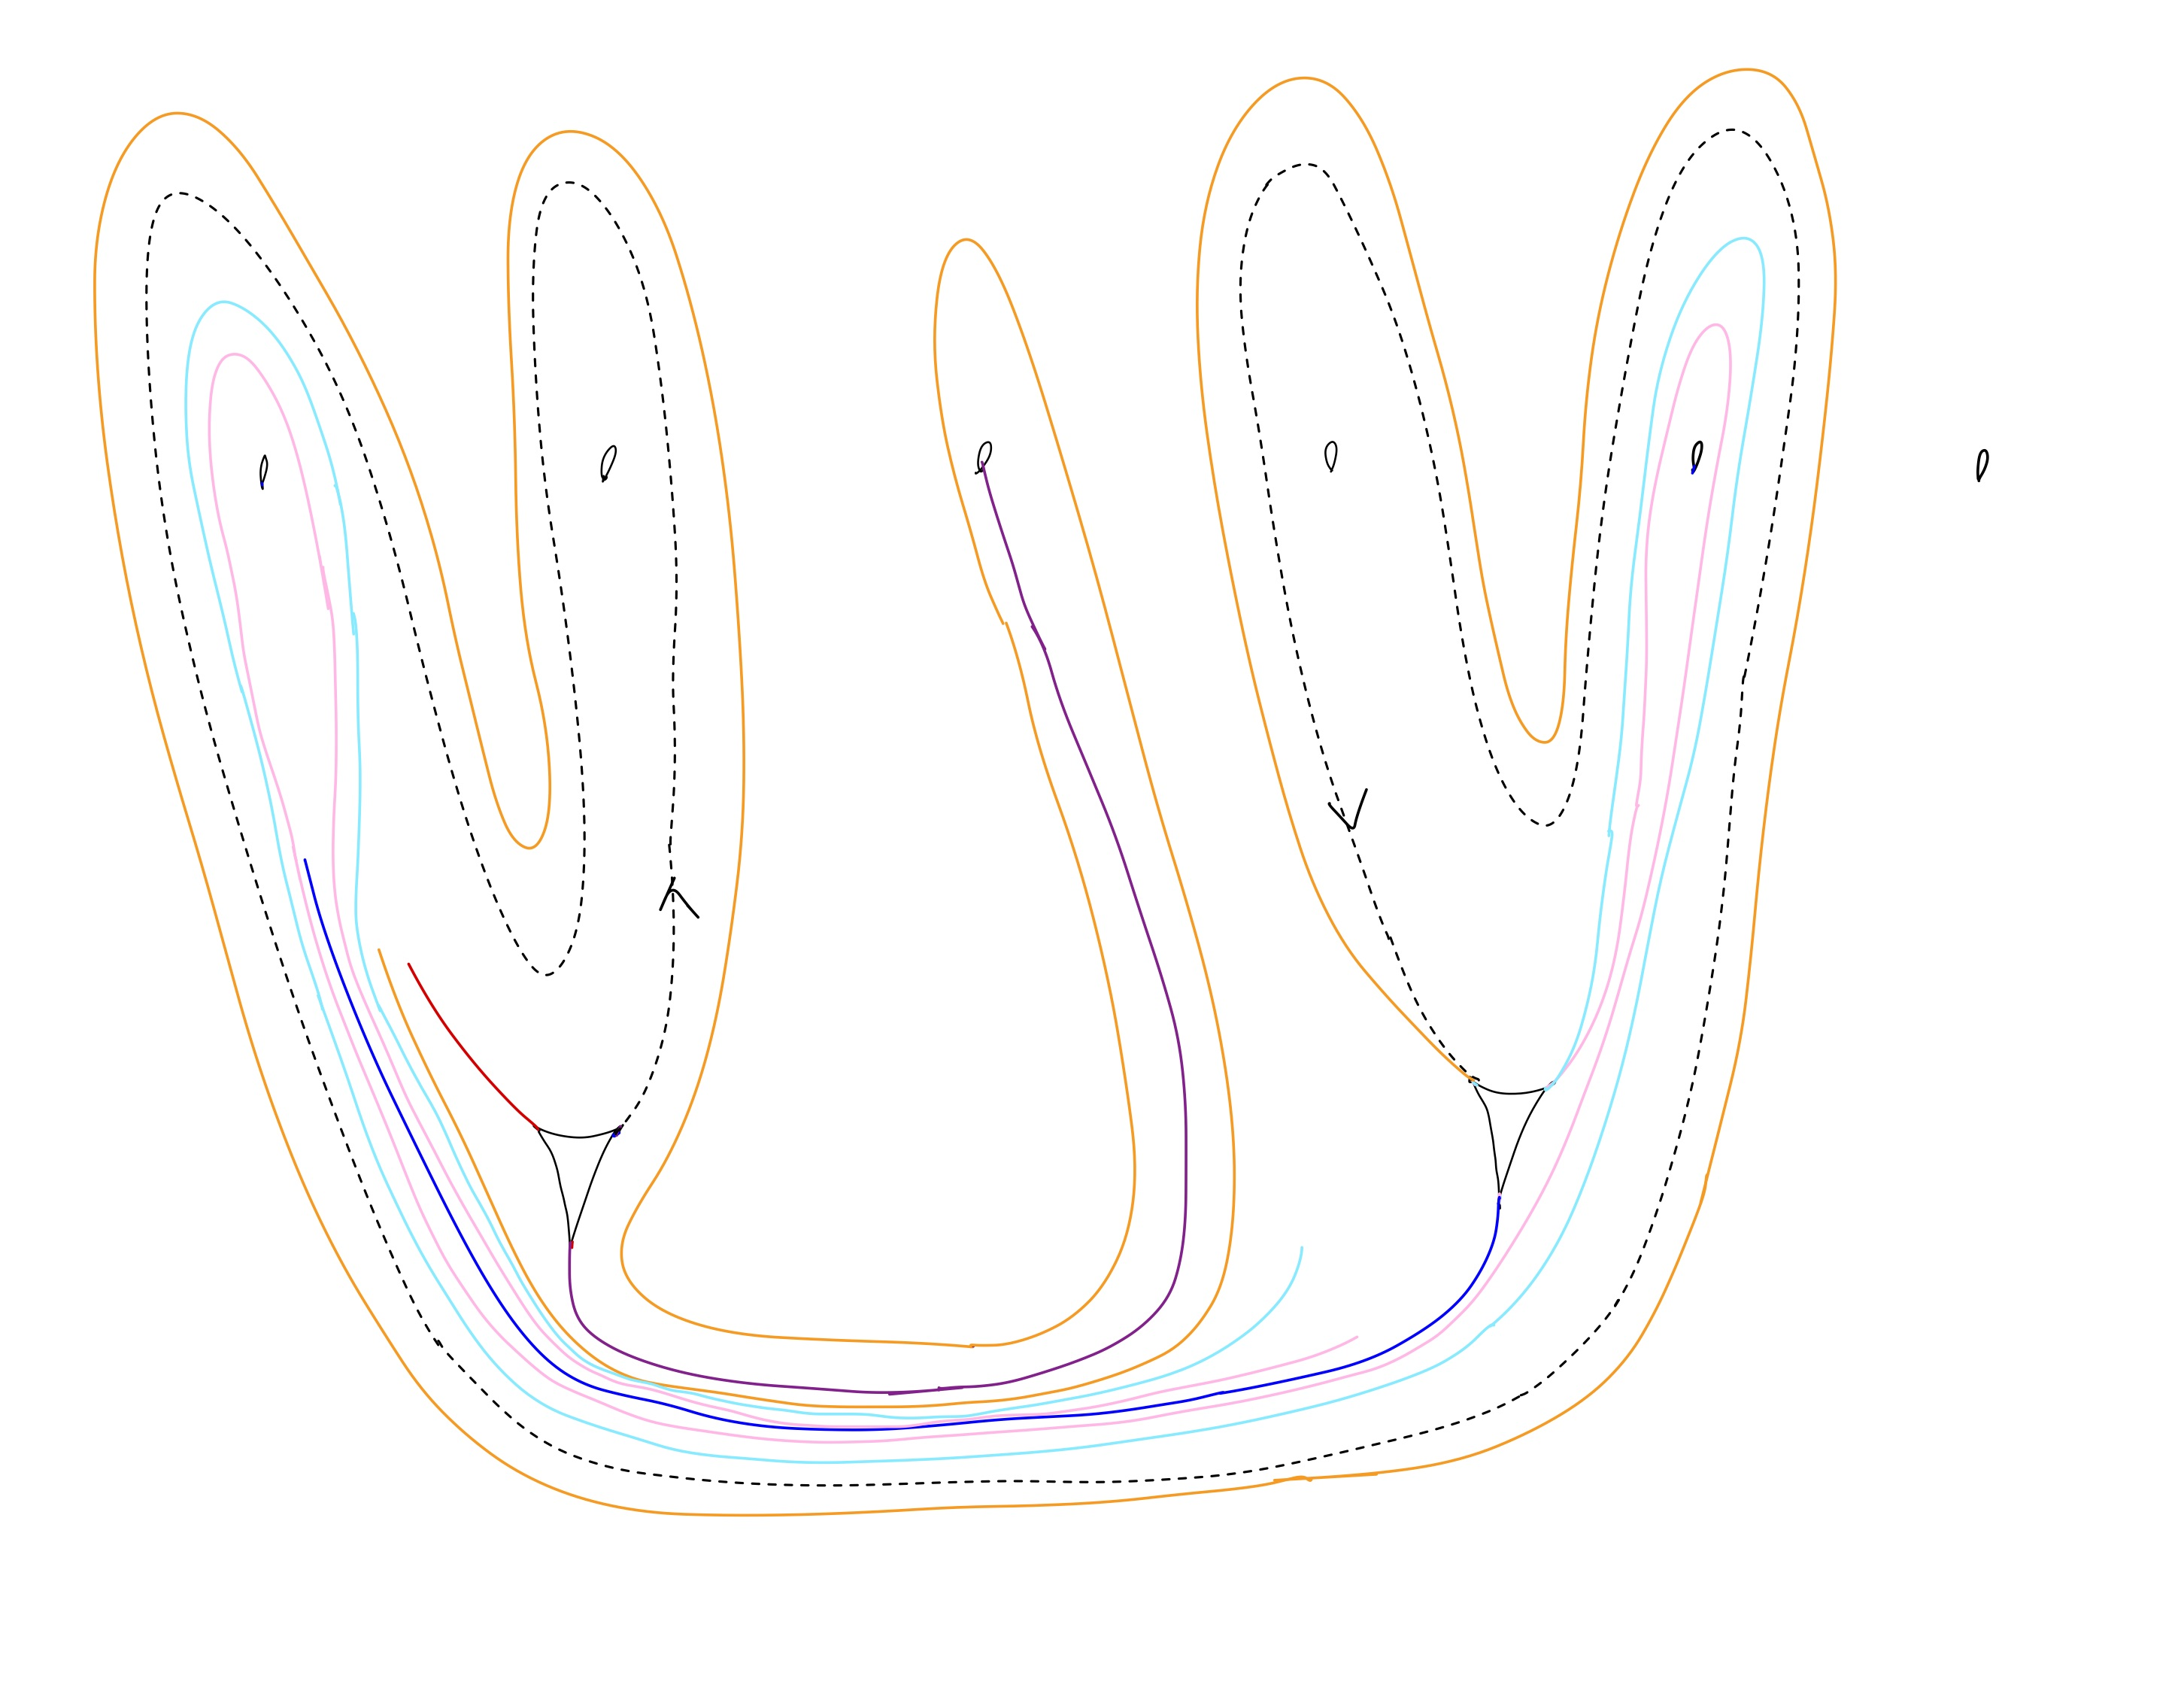
\includegraphics[width=\linewidth]{figures_case_analysis/track17_case_analysis/Roop-14.jpg}
    \caption{Roop14}
    \label{fig:Roop14}
\end{figure}
\clearpage

\begin{figure}[ht]
    \centering
    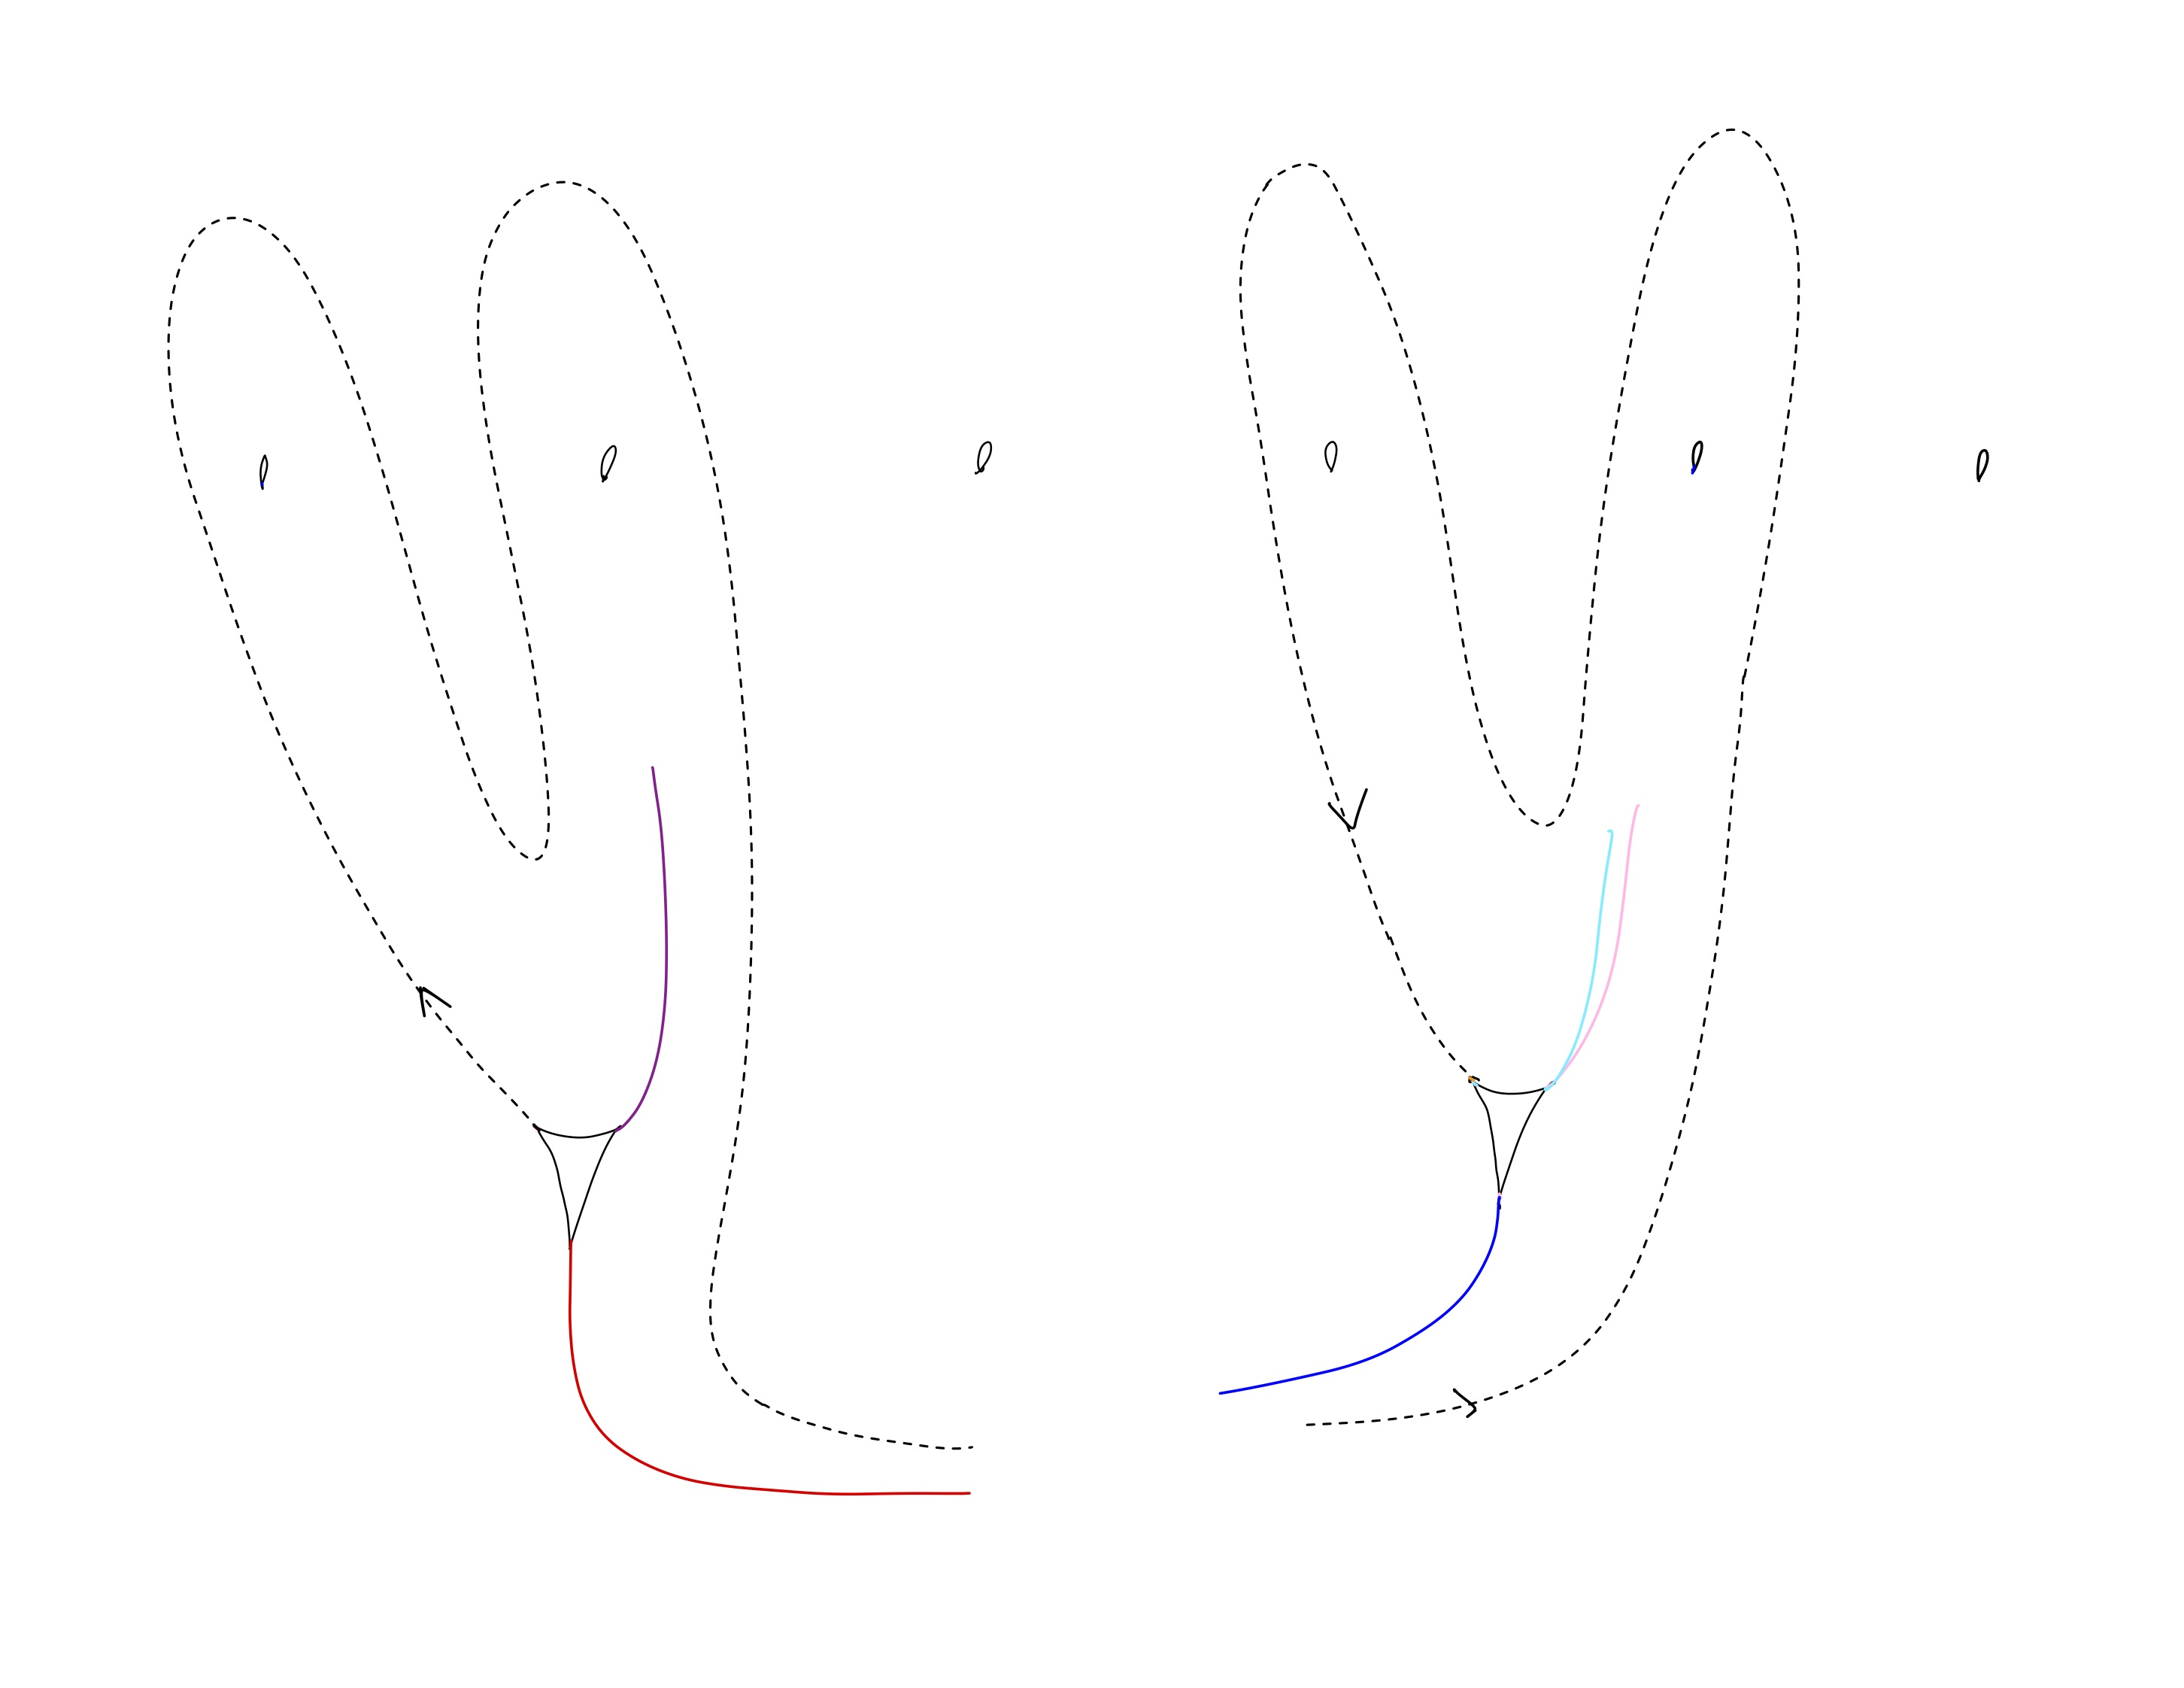
\includegraphics[width=\linewidth]{figures_case_analysis/track17_case_analysis/GKA-1.jpg}
    \caption{GKA1}
    \label{fig:GKA1}
\end{figure}

\begin{figure}[ht]
    \centering
    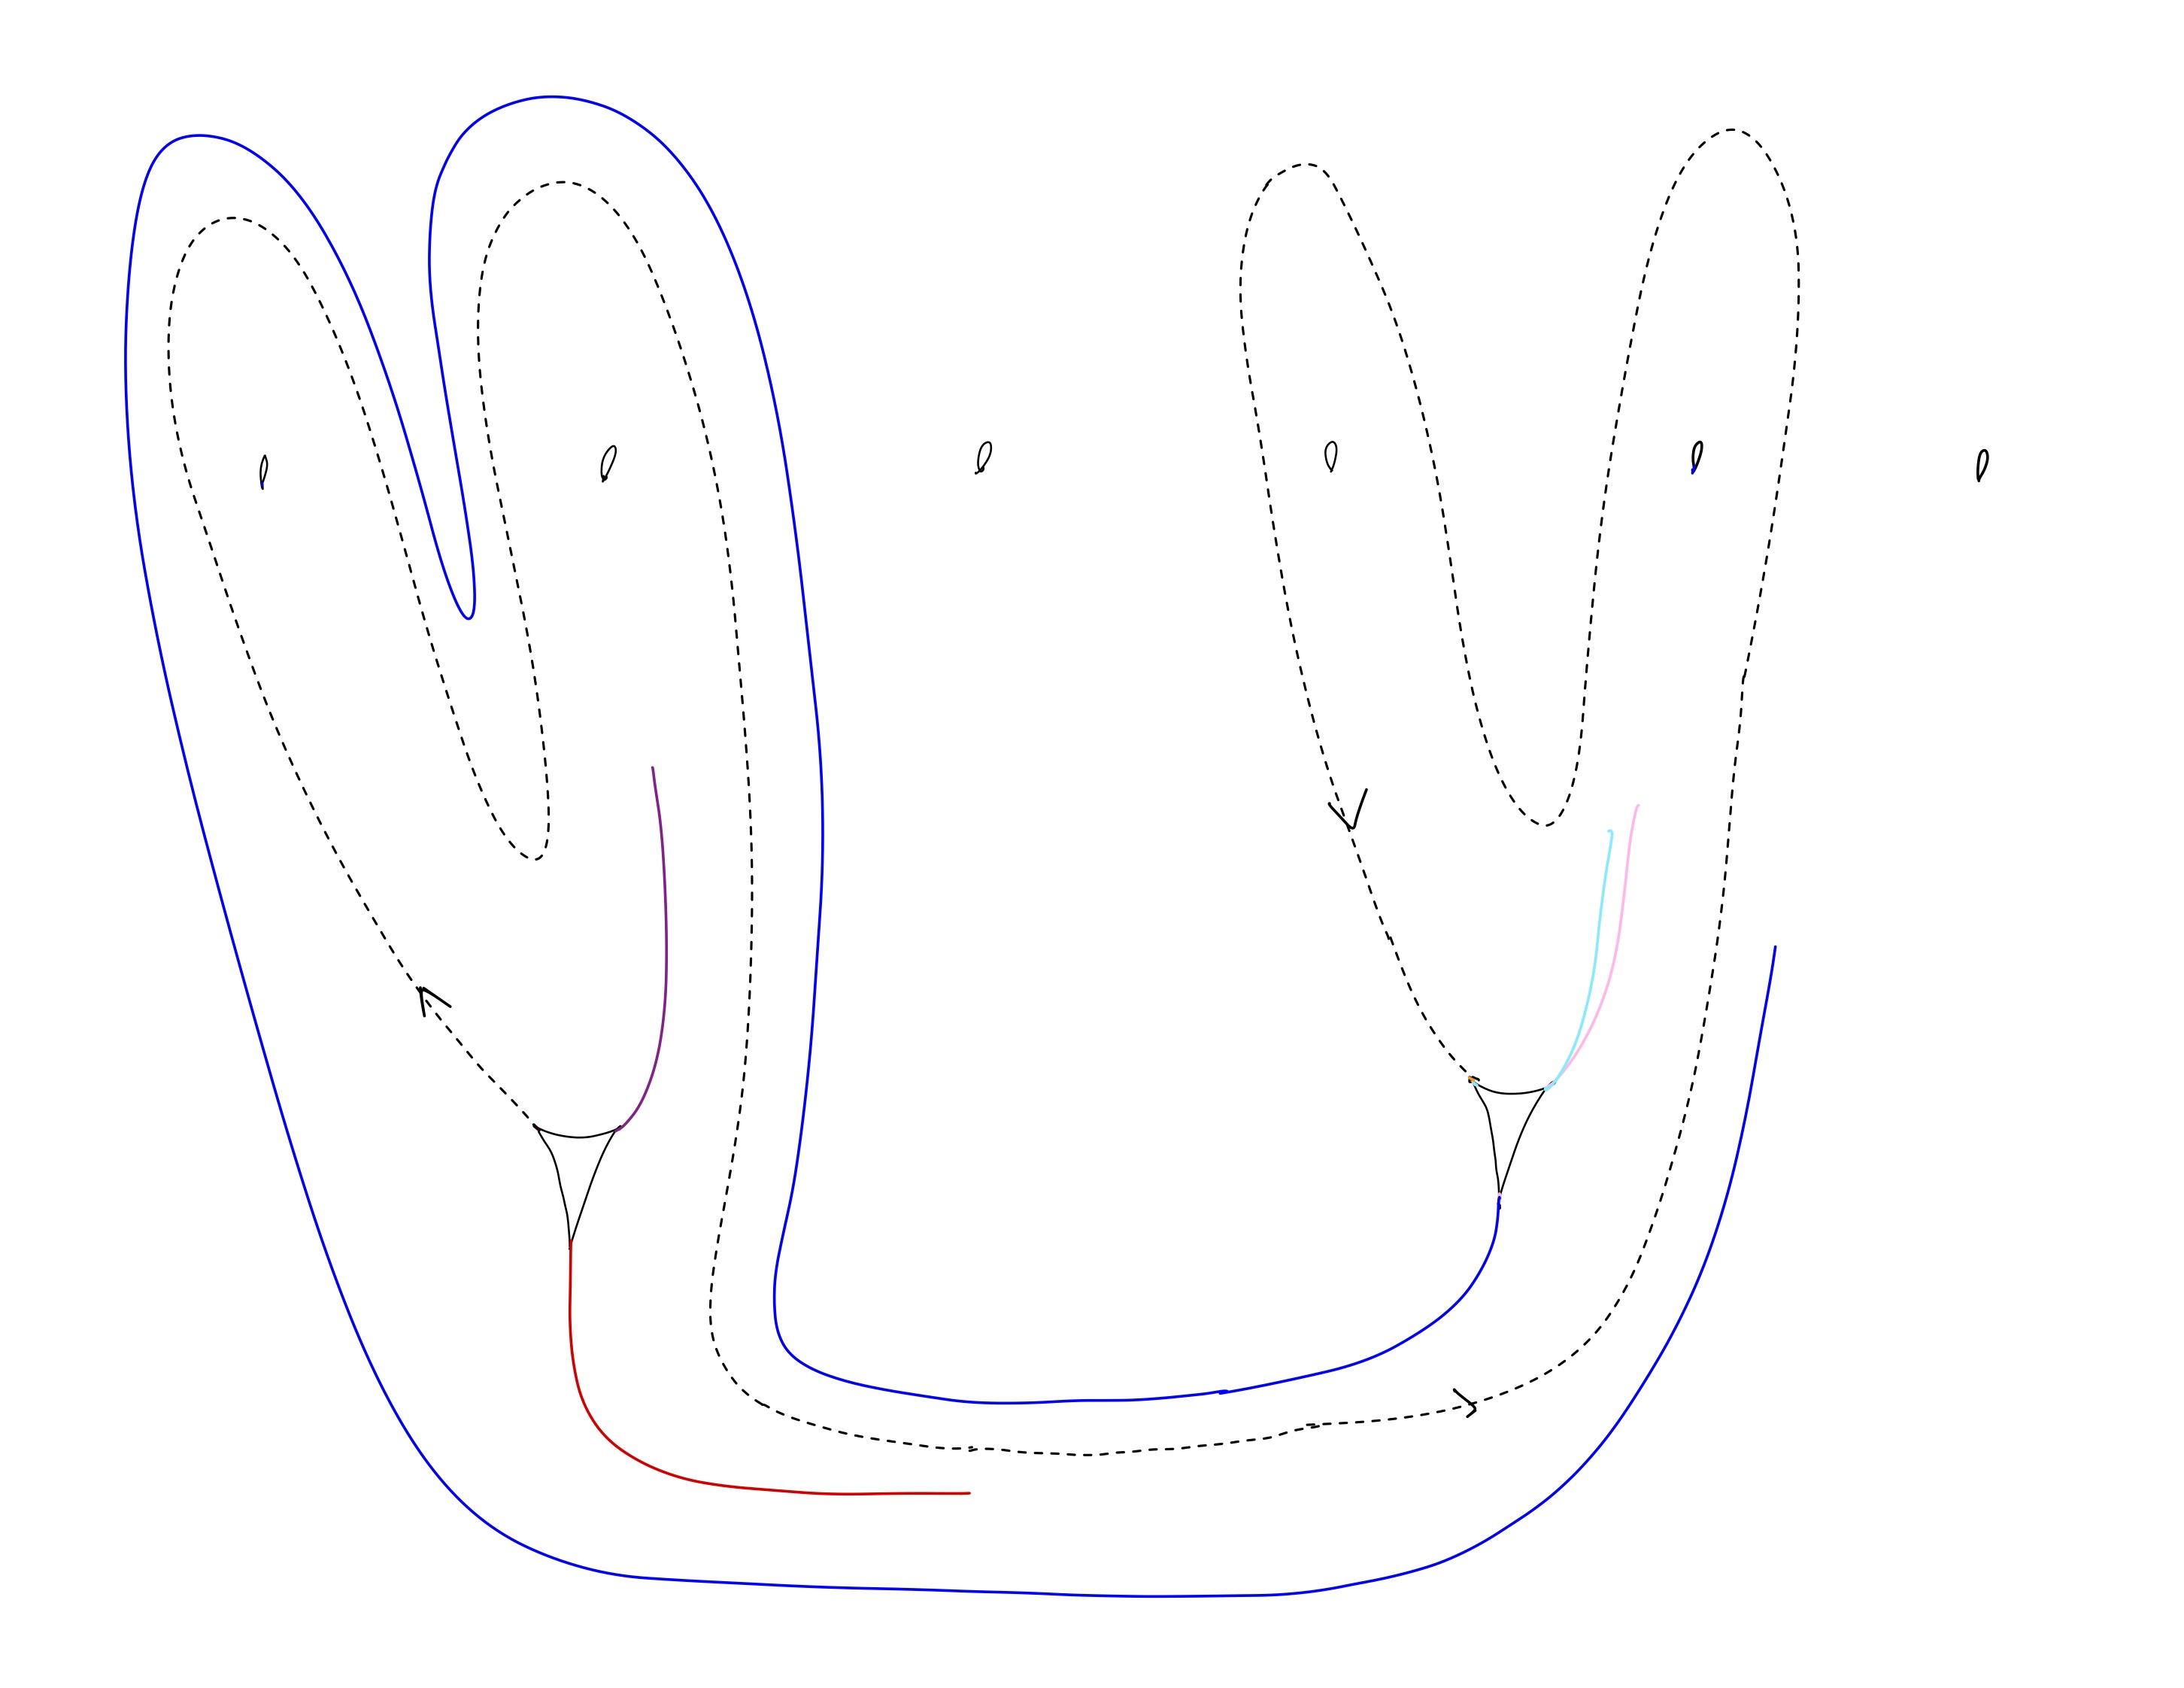
\includegraphics[width=\linewidth]{figures_case_analysis/track17_case_analysis/GKA-2.jpg}
    \caption{GKA2}
    \label{fig:GKA2}
\end{figure}

\begin{figure}[ht]
    \centering
    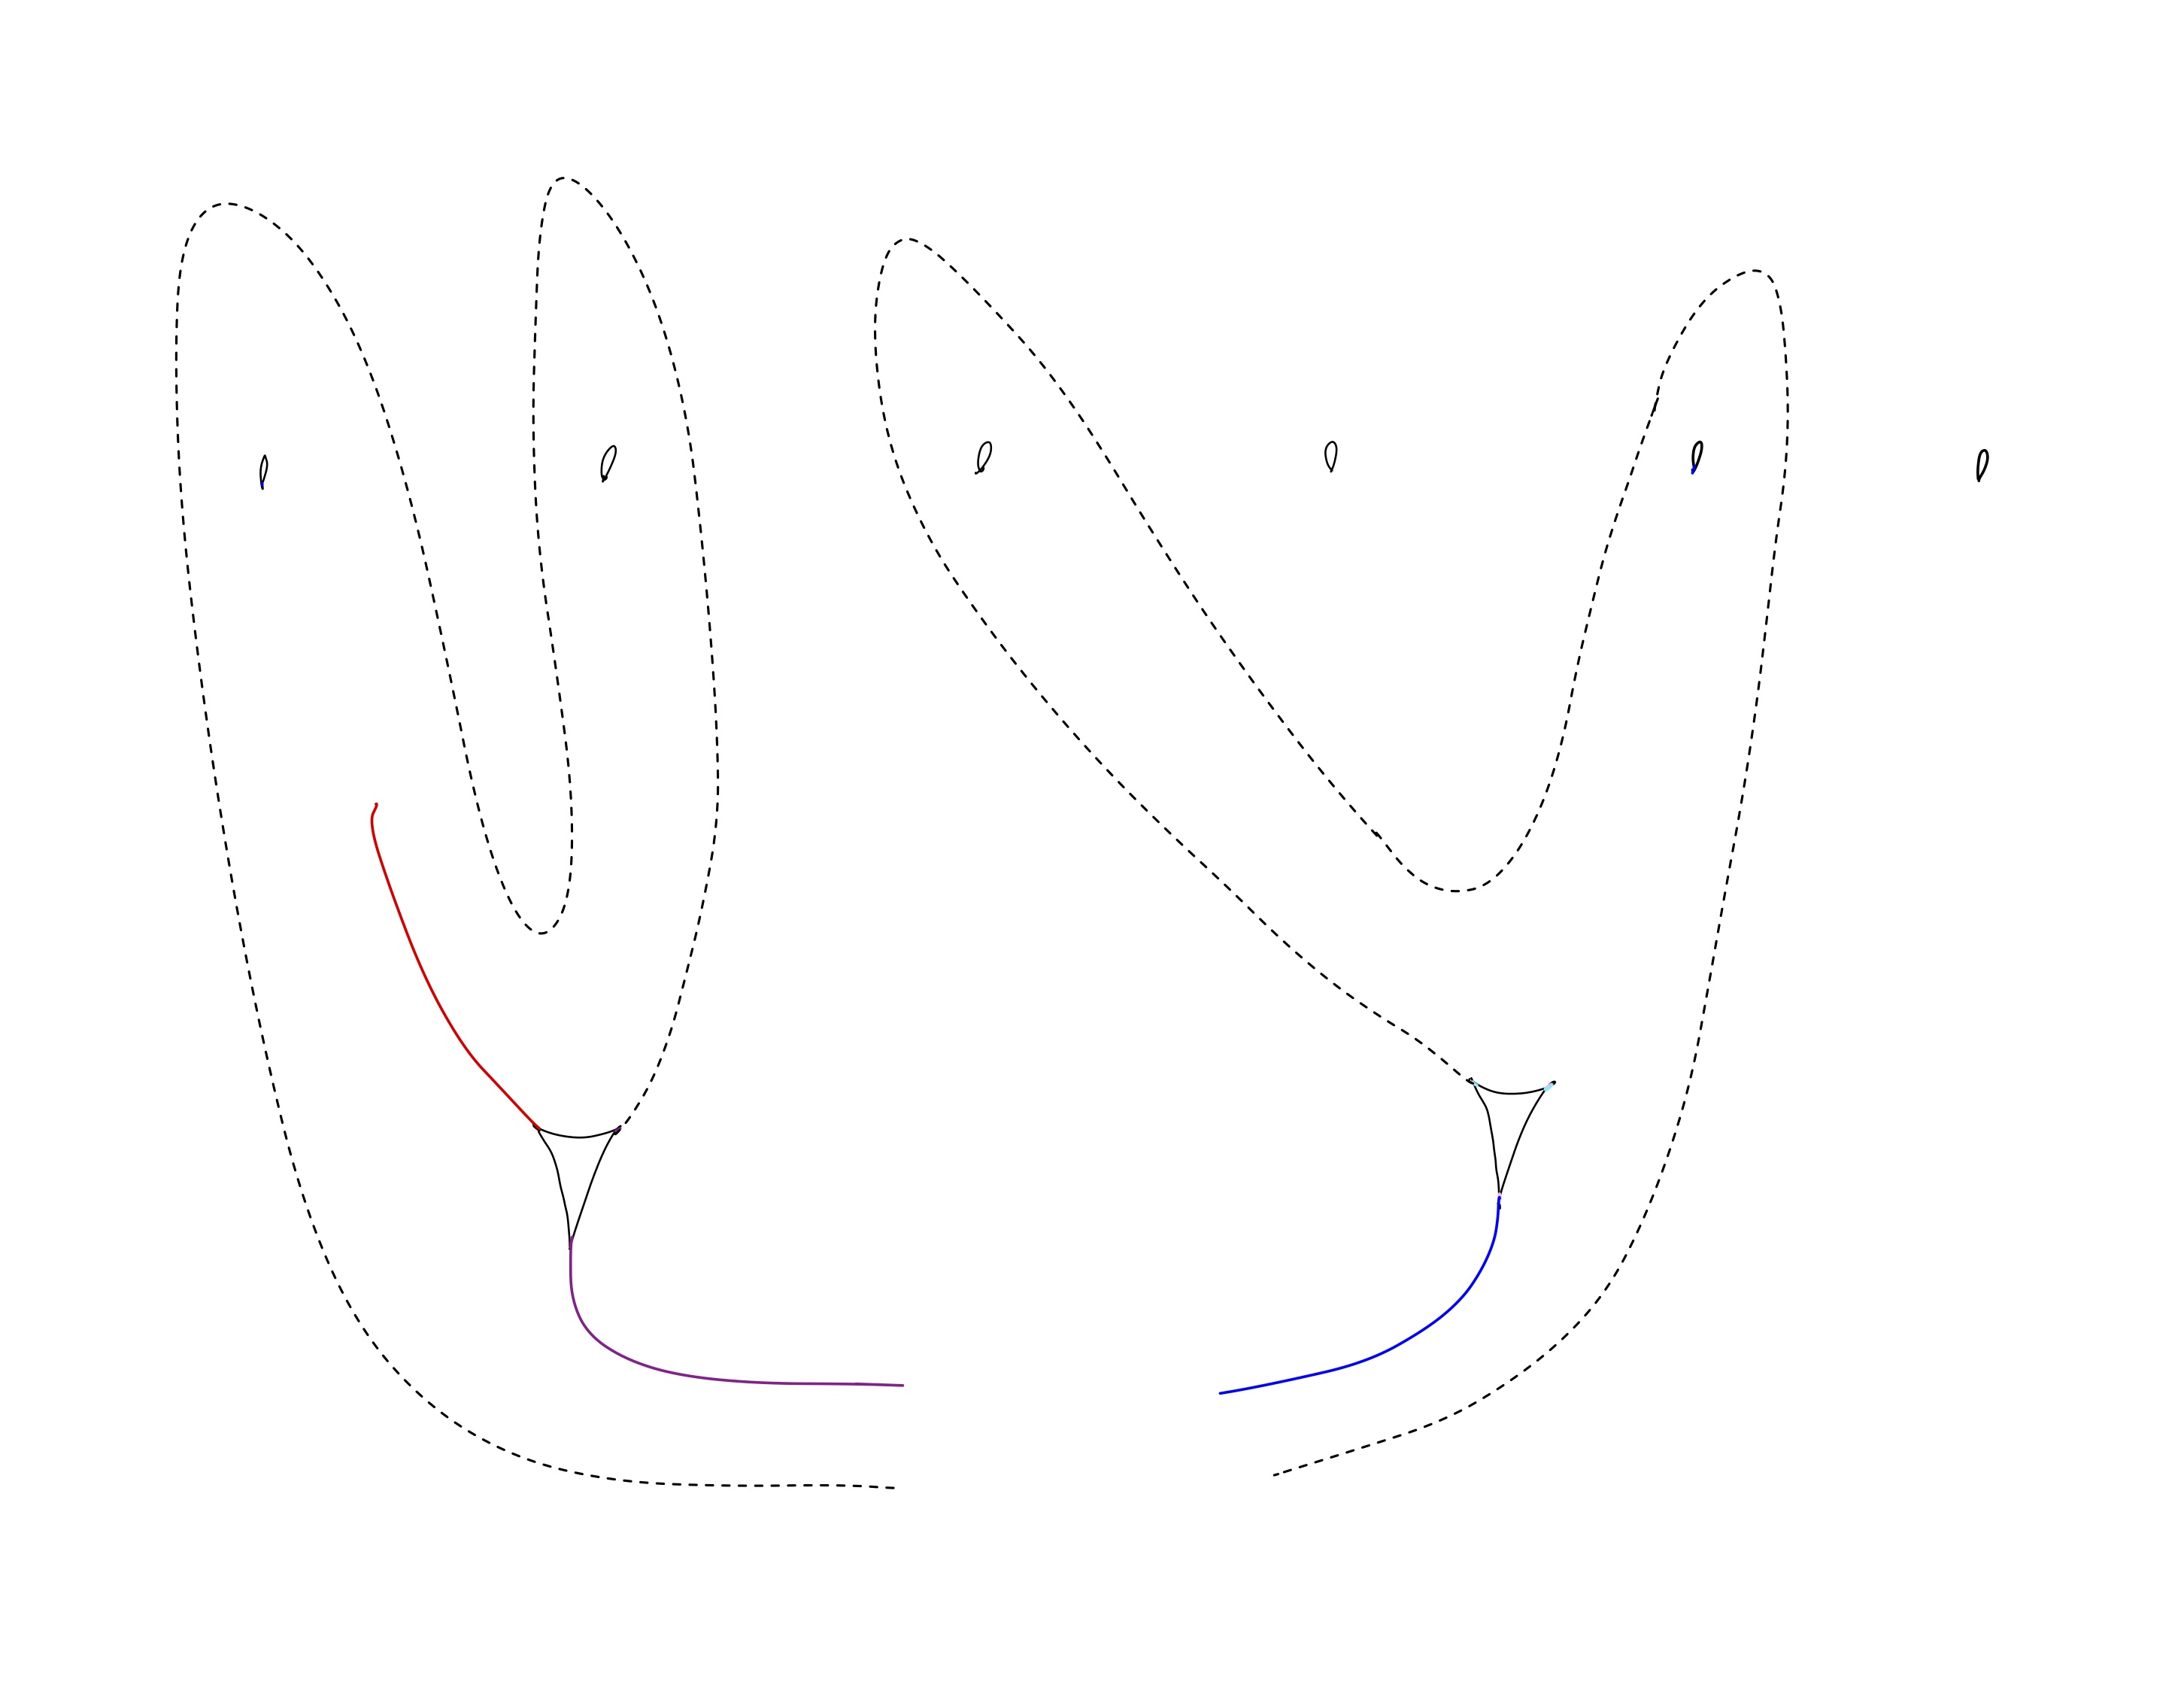
\includegraphics[width=\linewidth]{figures_case_analysis/track17_case_analysis/WGA-1.jpg}
    \caption{WGA1}
    \label{fig:WGA1}
\end{figure}

\begin{figure}[ht]
    \centering
    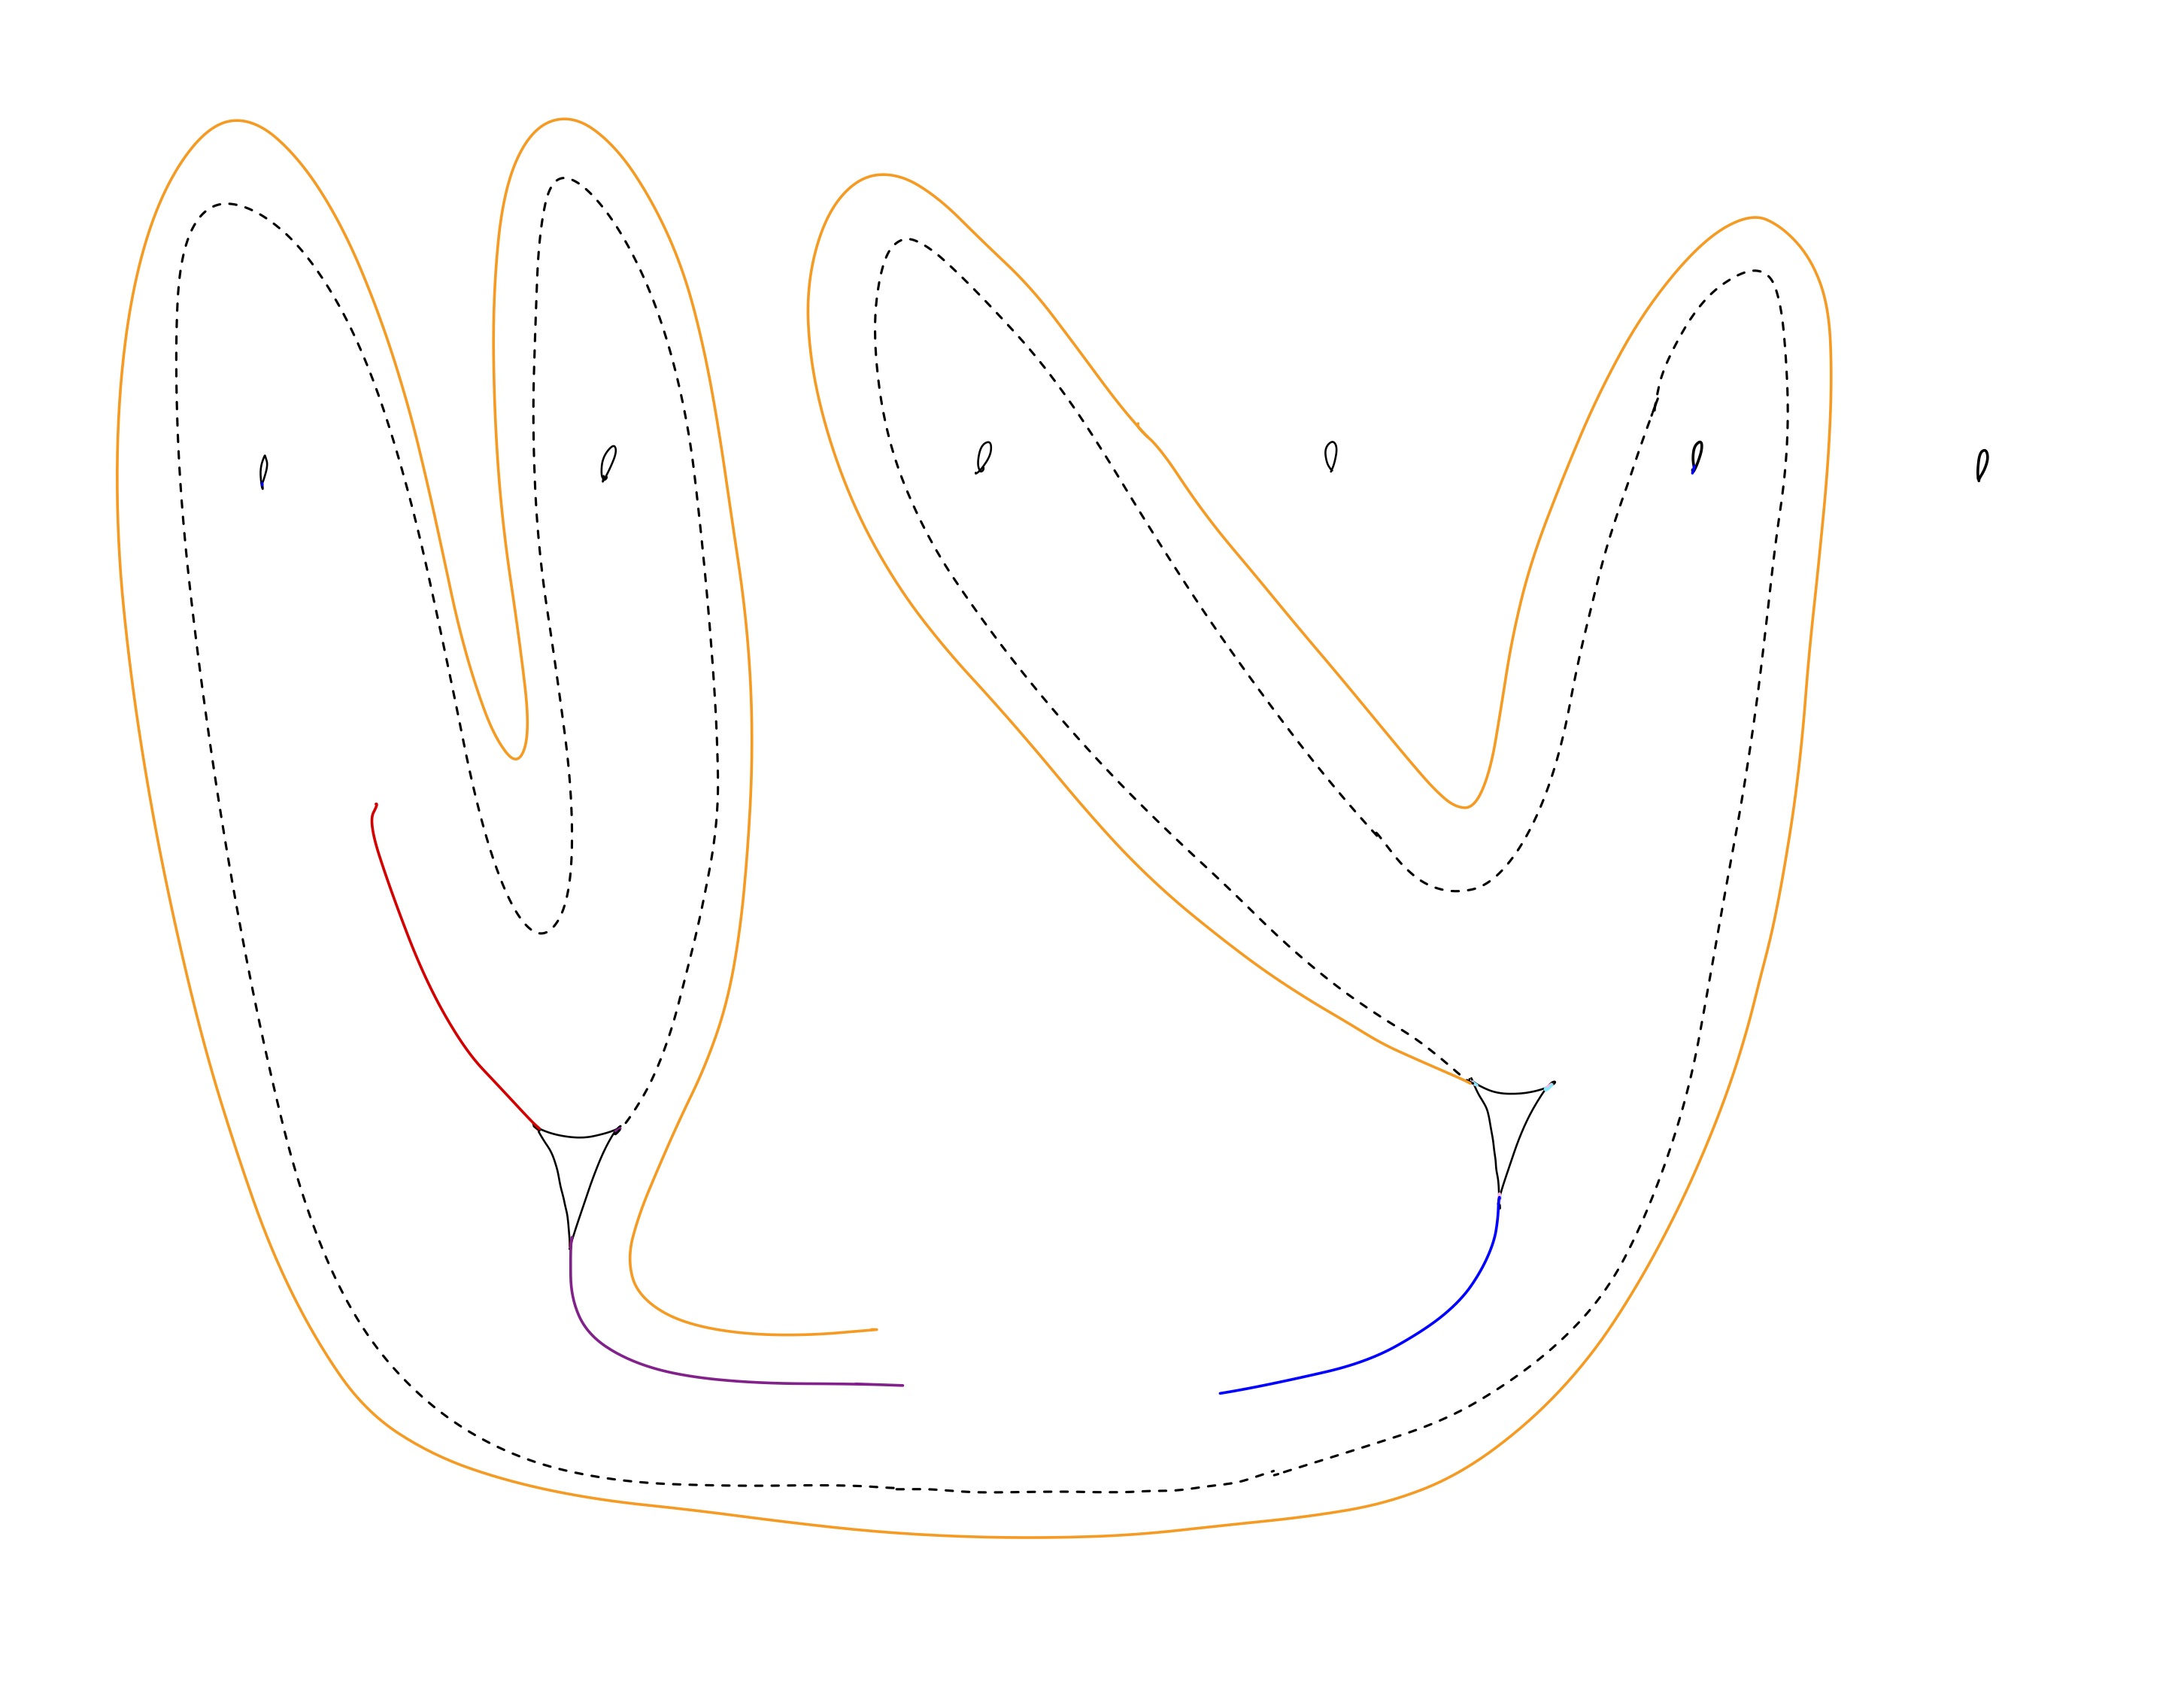
\includegraphics[width=\linewidth]{figures_case_analysis/track17_case_analysis/WGA-2.jpg}
    \caption{WGA2}
    \label{fig:WGA2}
\end{figure}

\begin{figure}[ht]
    \centering
    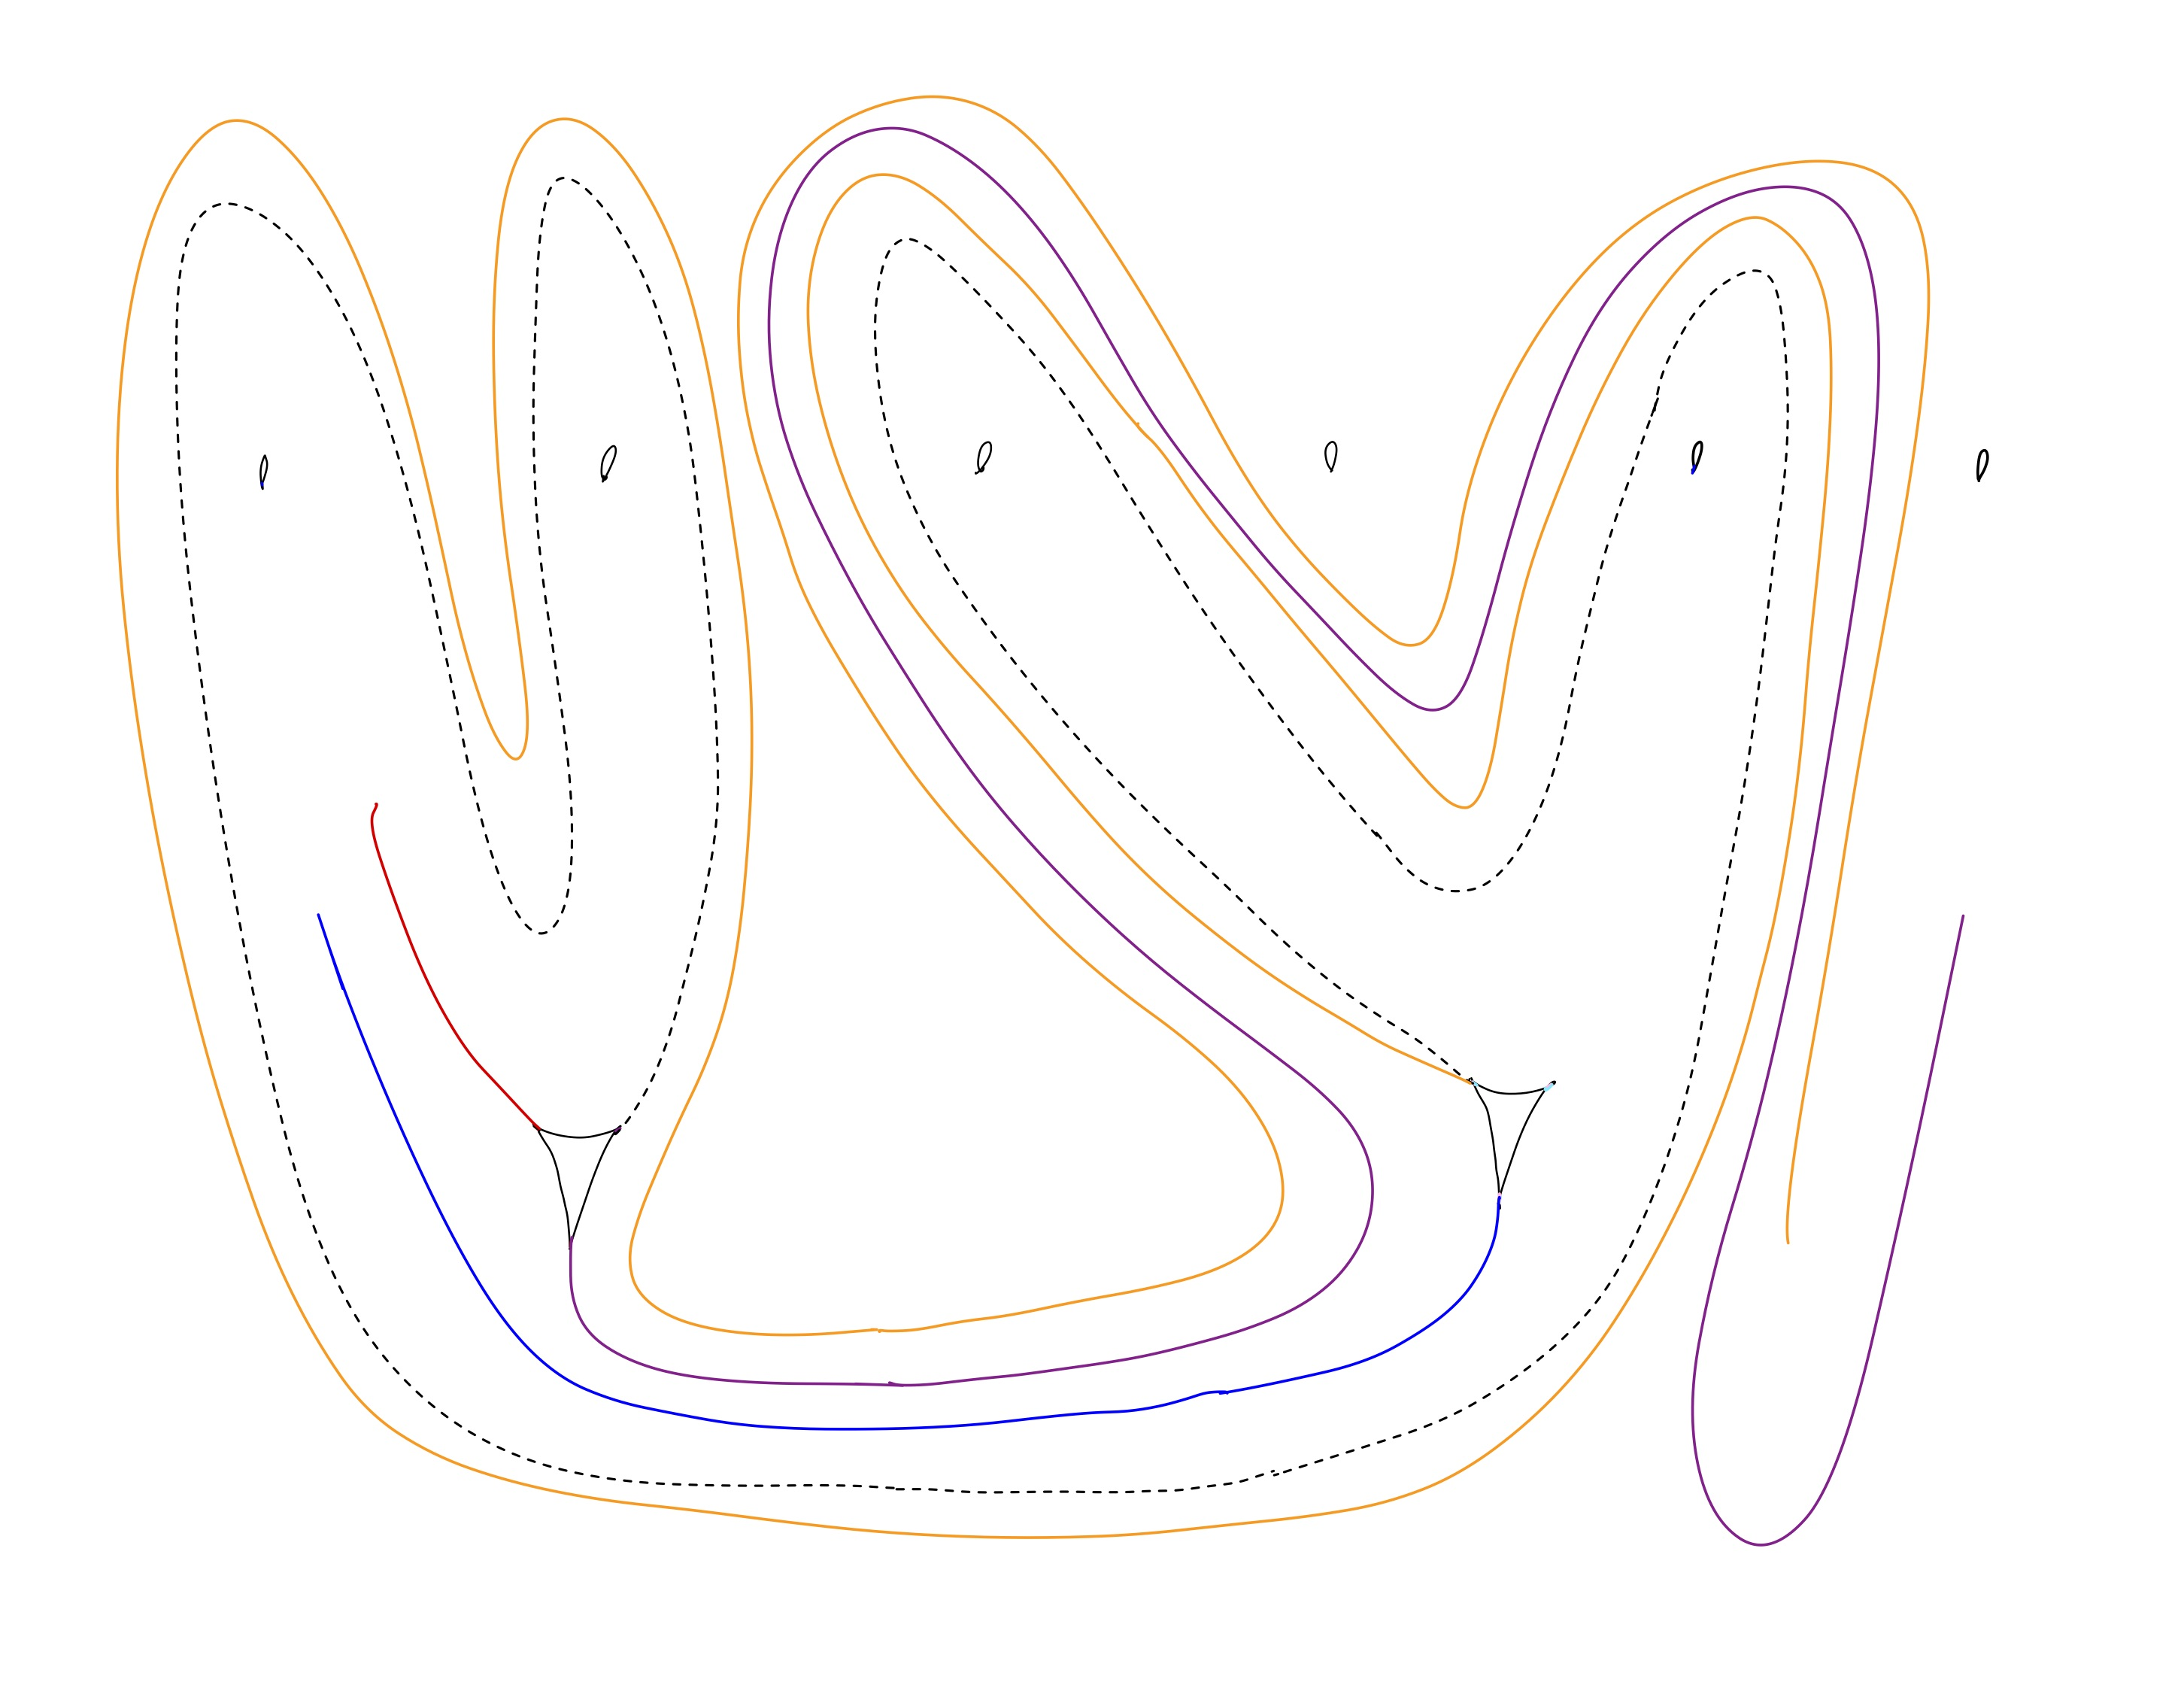
\includegraphics[width=\linewidth]{figures_case_analysis/track17_case_analysis/WGA-3.jpg}
    \caption{WGA3}
    \label{fig:WGA3}
\end{figure}

\clearpage

\begin{figure}[ht]
    \centering
    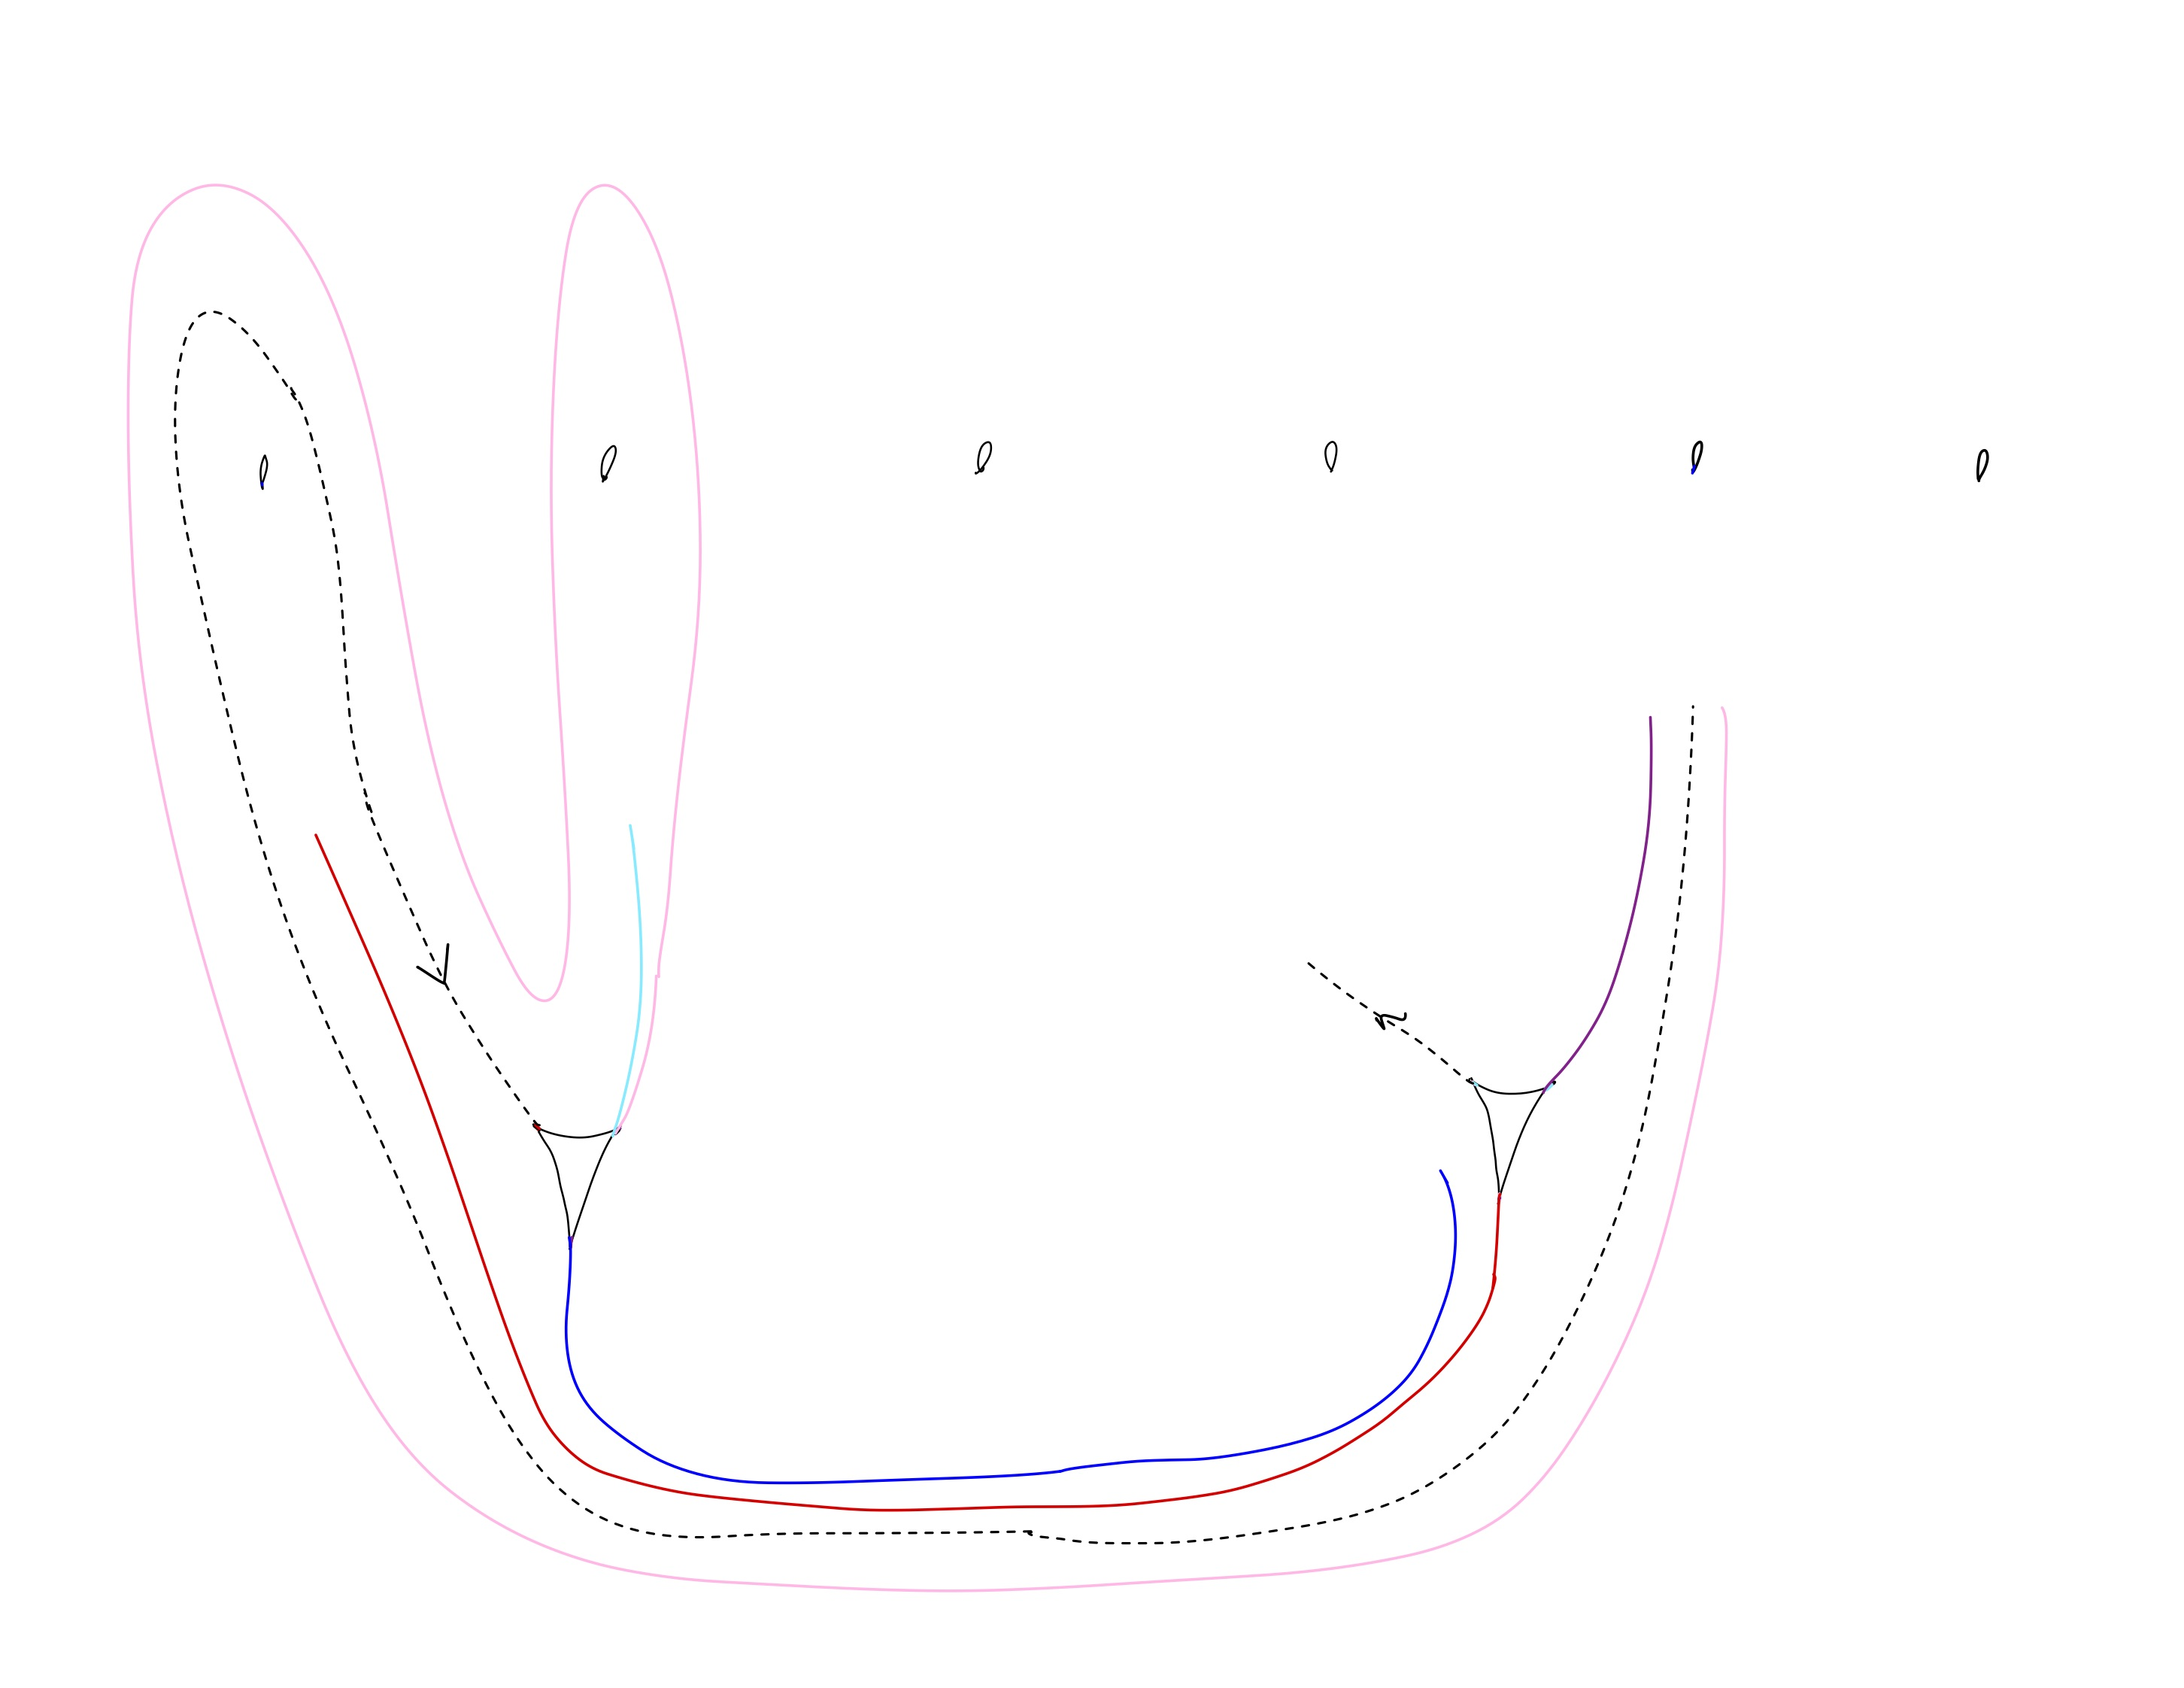
\includegraphics[width=\linewidth]{figures_case_analysis/track17_case_analysis/GBR-01.jpg}
    \caption{GBR1}
    \label{fig:GBR1}
\end{figure}

\begin{figure}[ht]
    \centering
    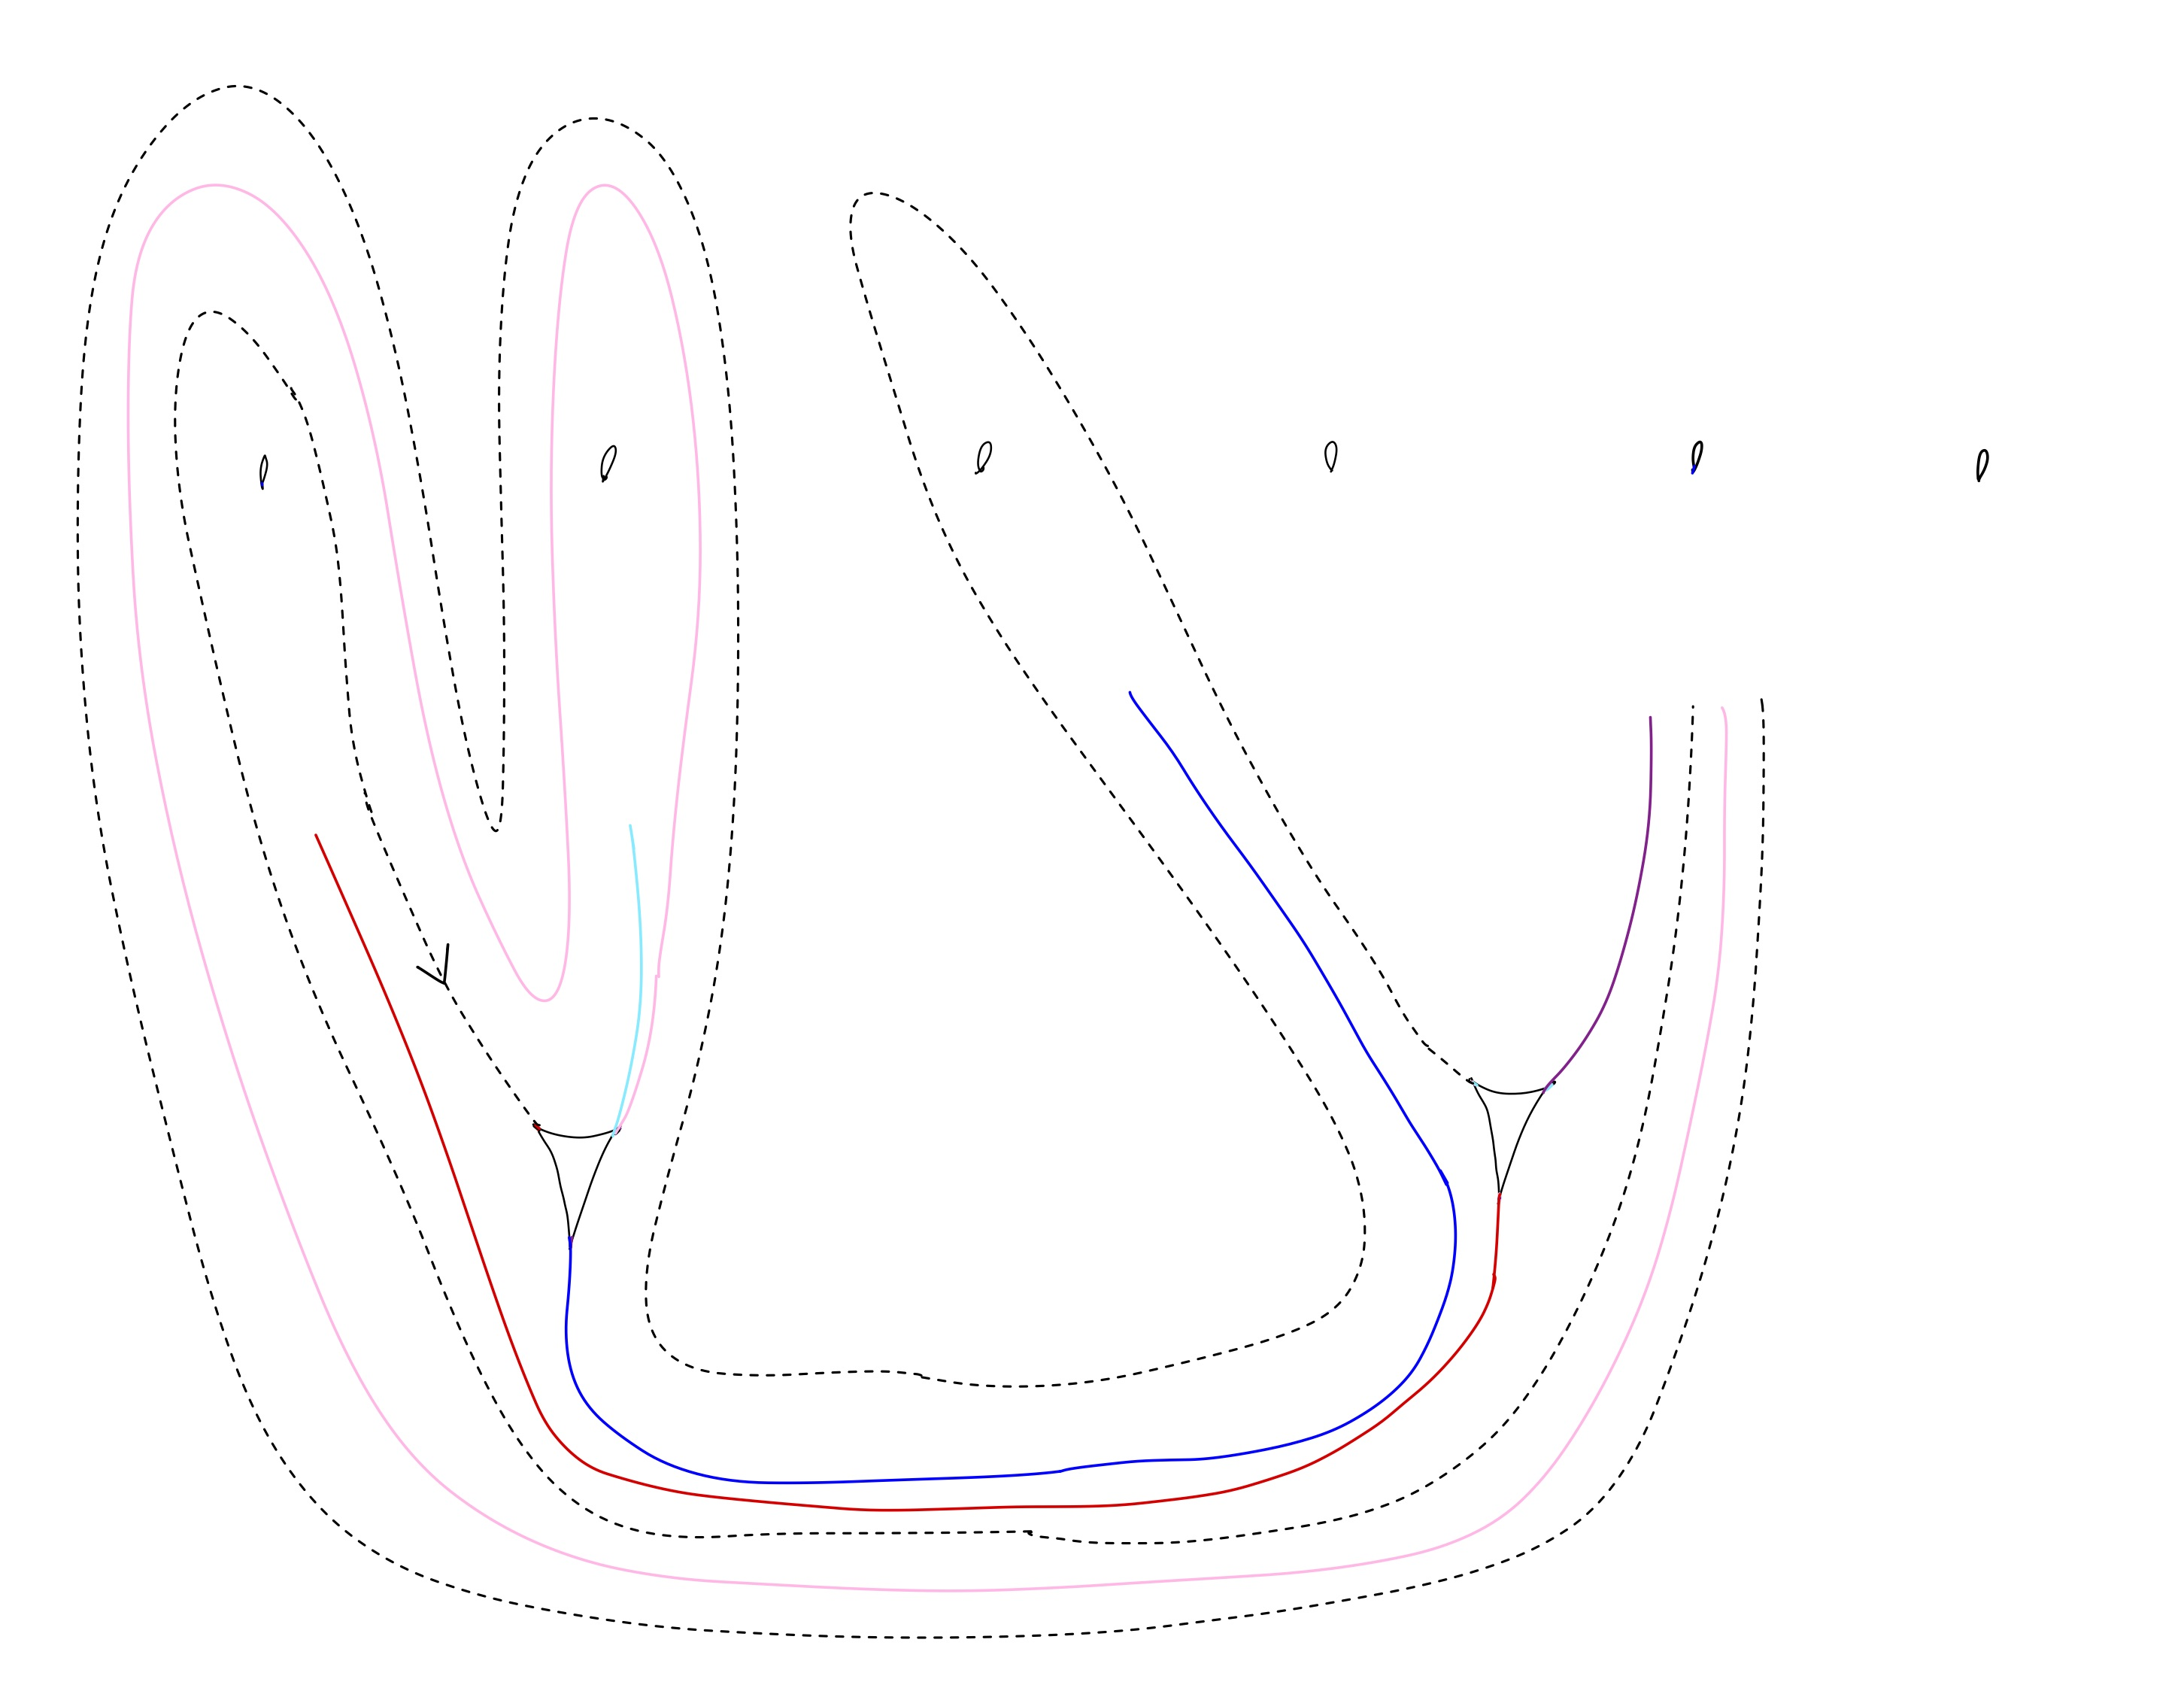
\includegraphics[width=\linewidth]{figures_case_analysis/track17_case_analysis/GBR-02.jpg}
    \caption{GBR2}
    \label{fig:GBR2}
\end{figure}

\begin{figure}[ht]
    \centering
    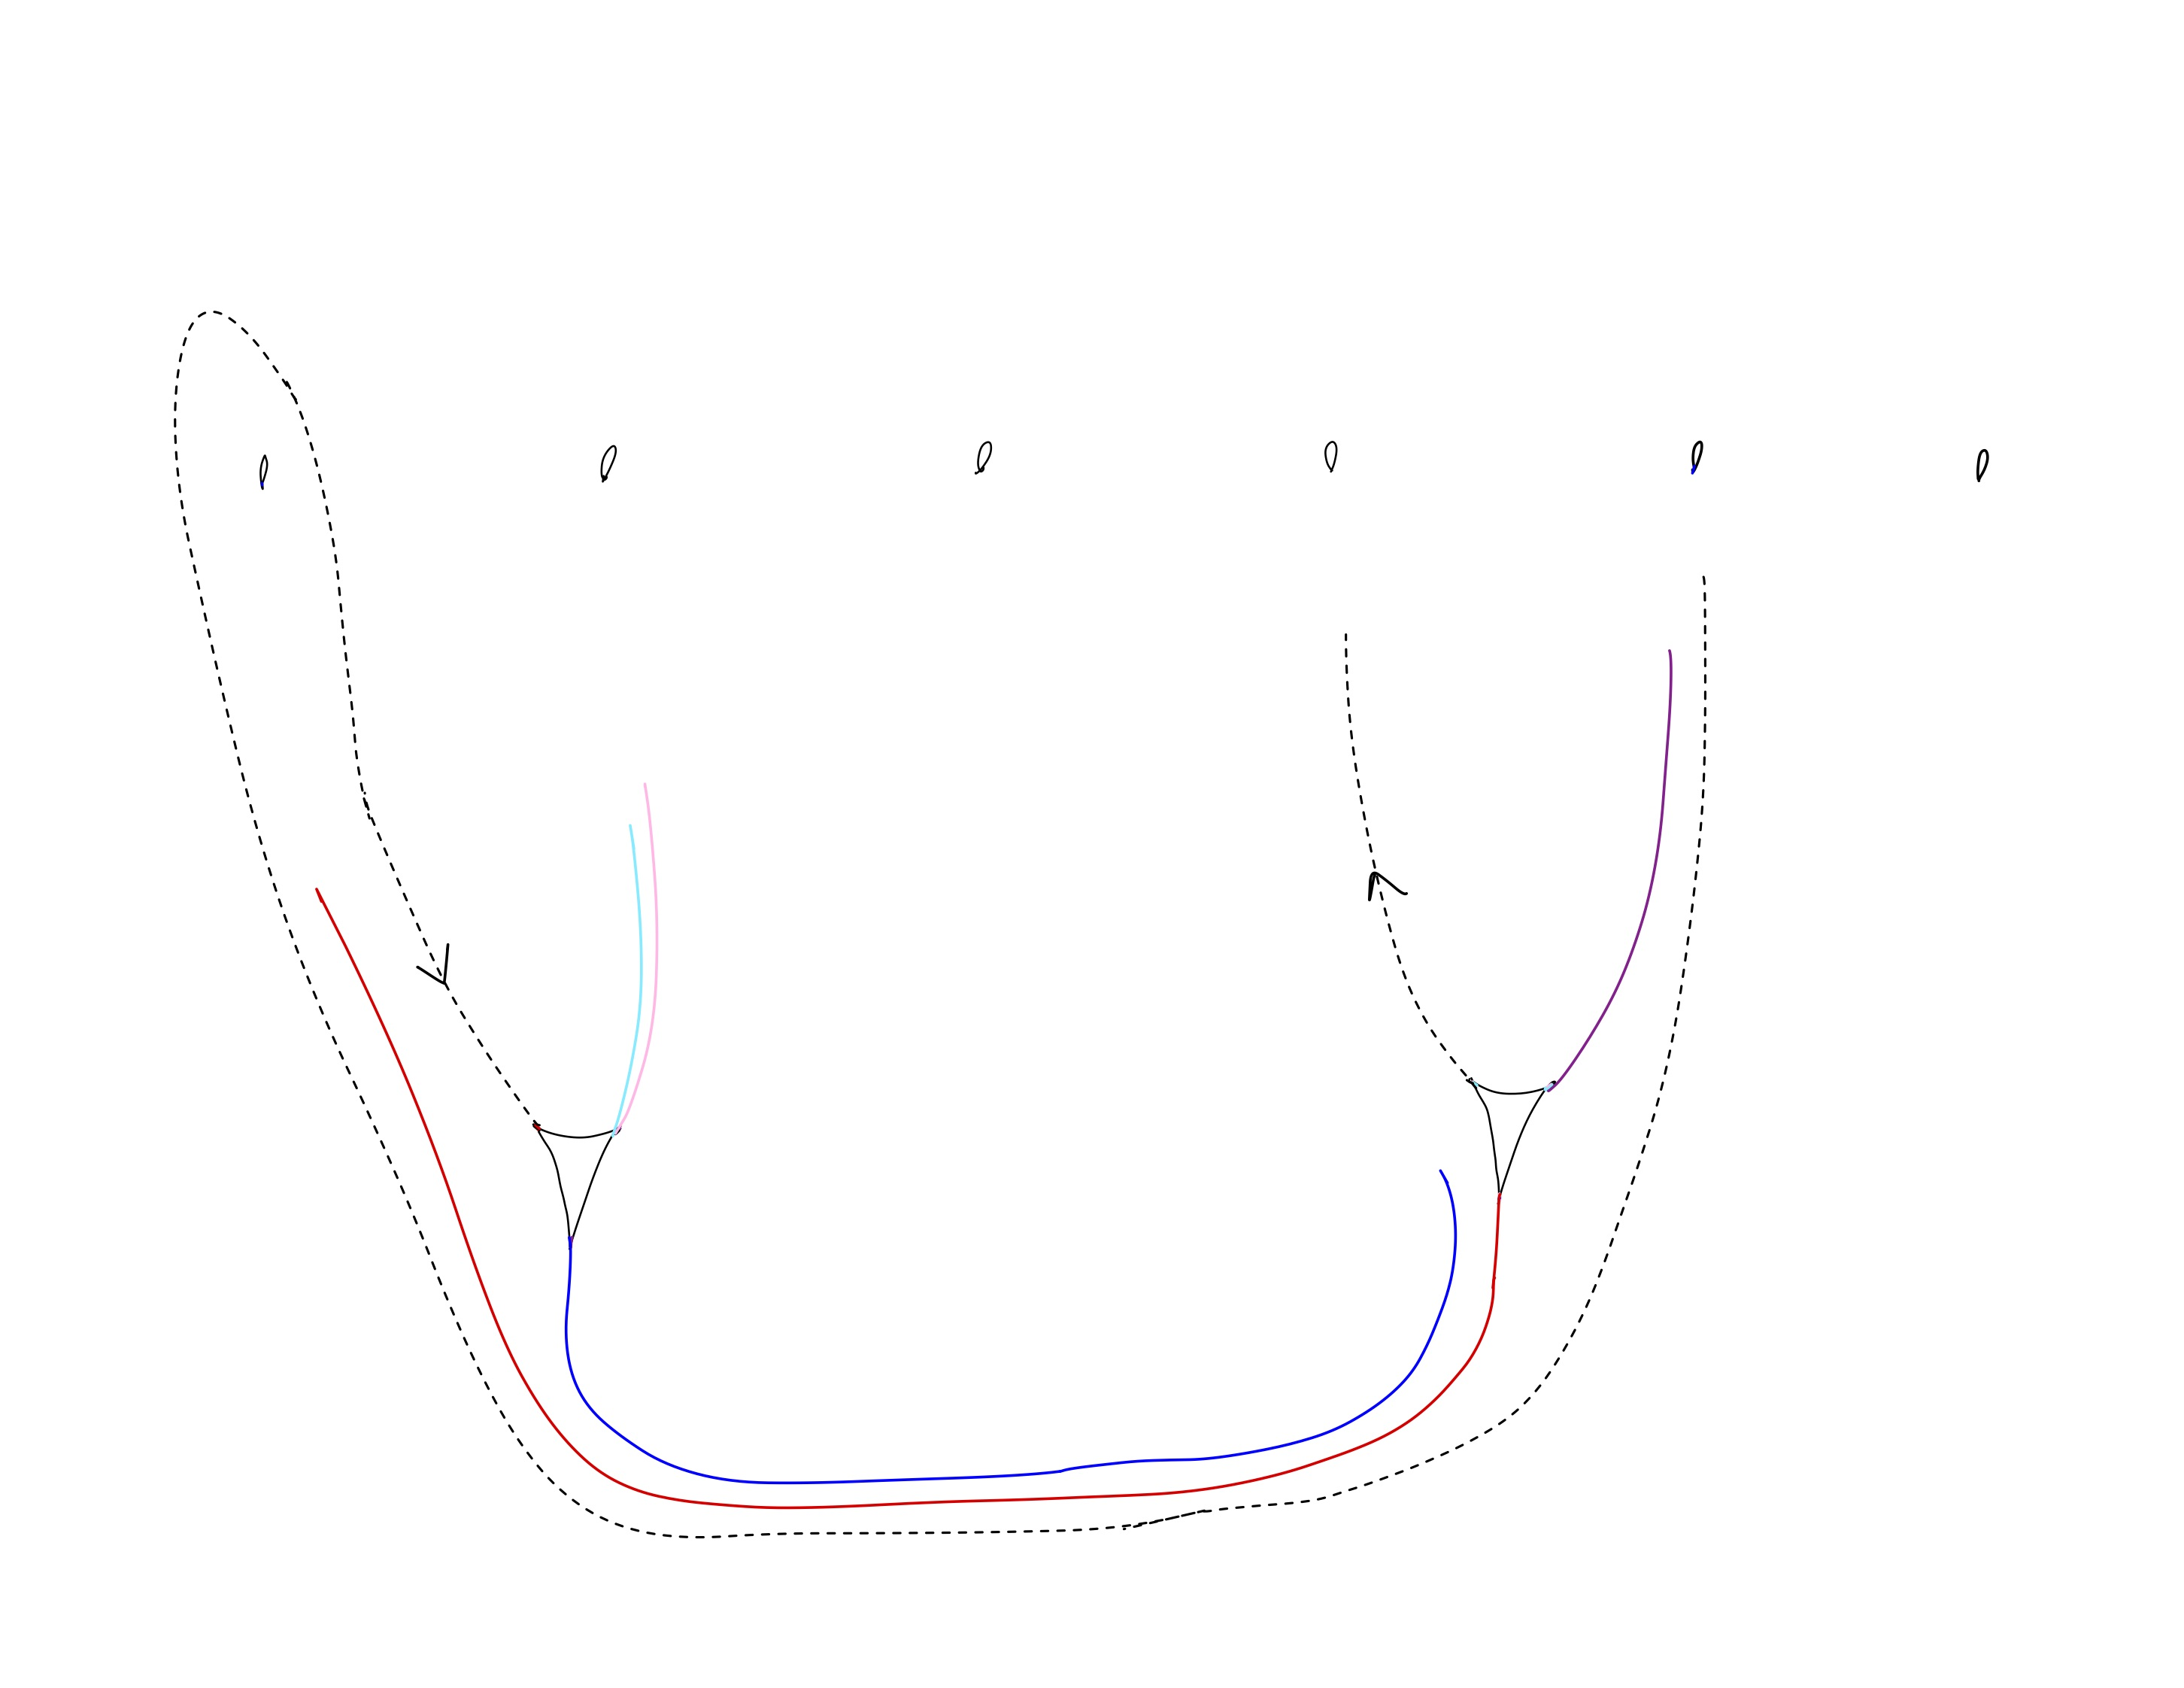
\includegraphics[width=\linewidth]{figures_case_analysis/track17_case_analysis/GBR-03.jpg}
    \caption{GBR3}
    \label{fig:GBR3}
\end{figure}

\begin{figure}[ht]
    \centering
    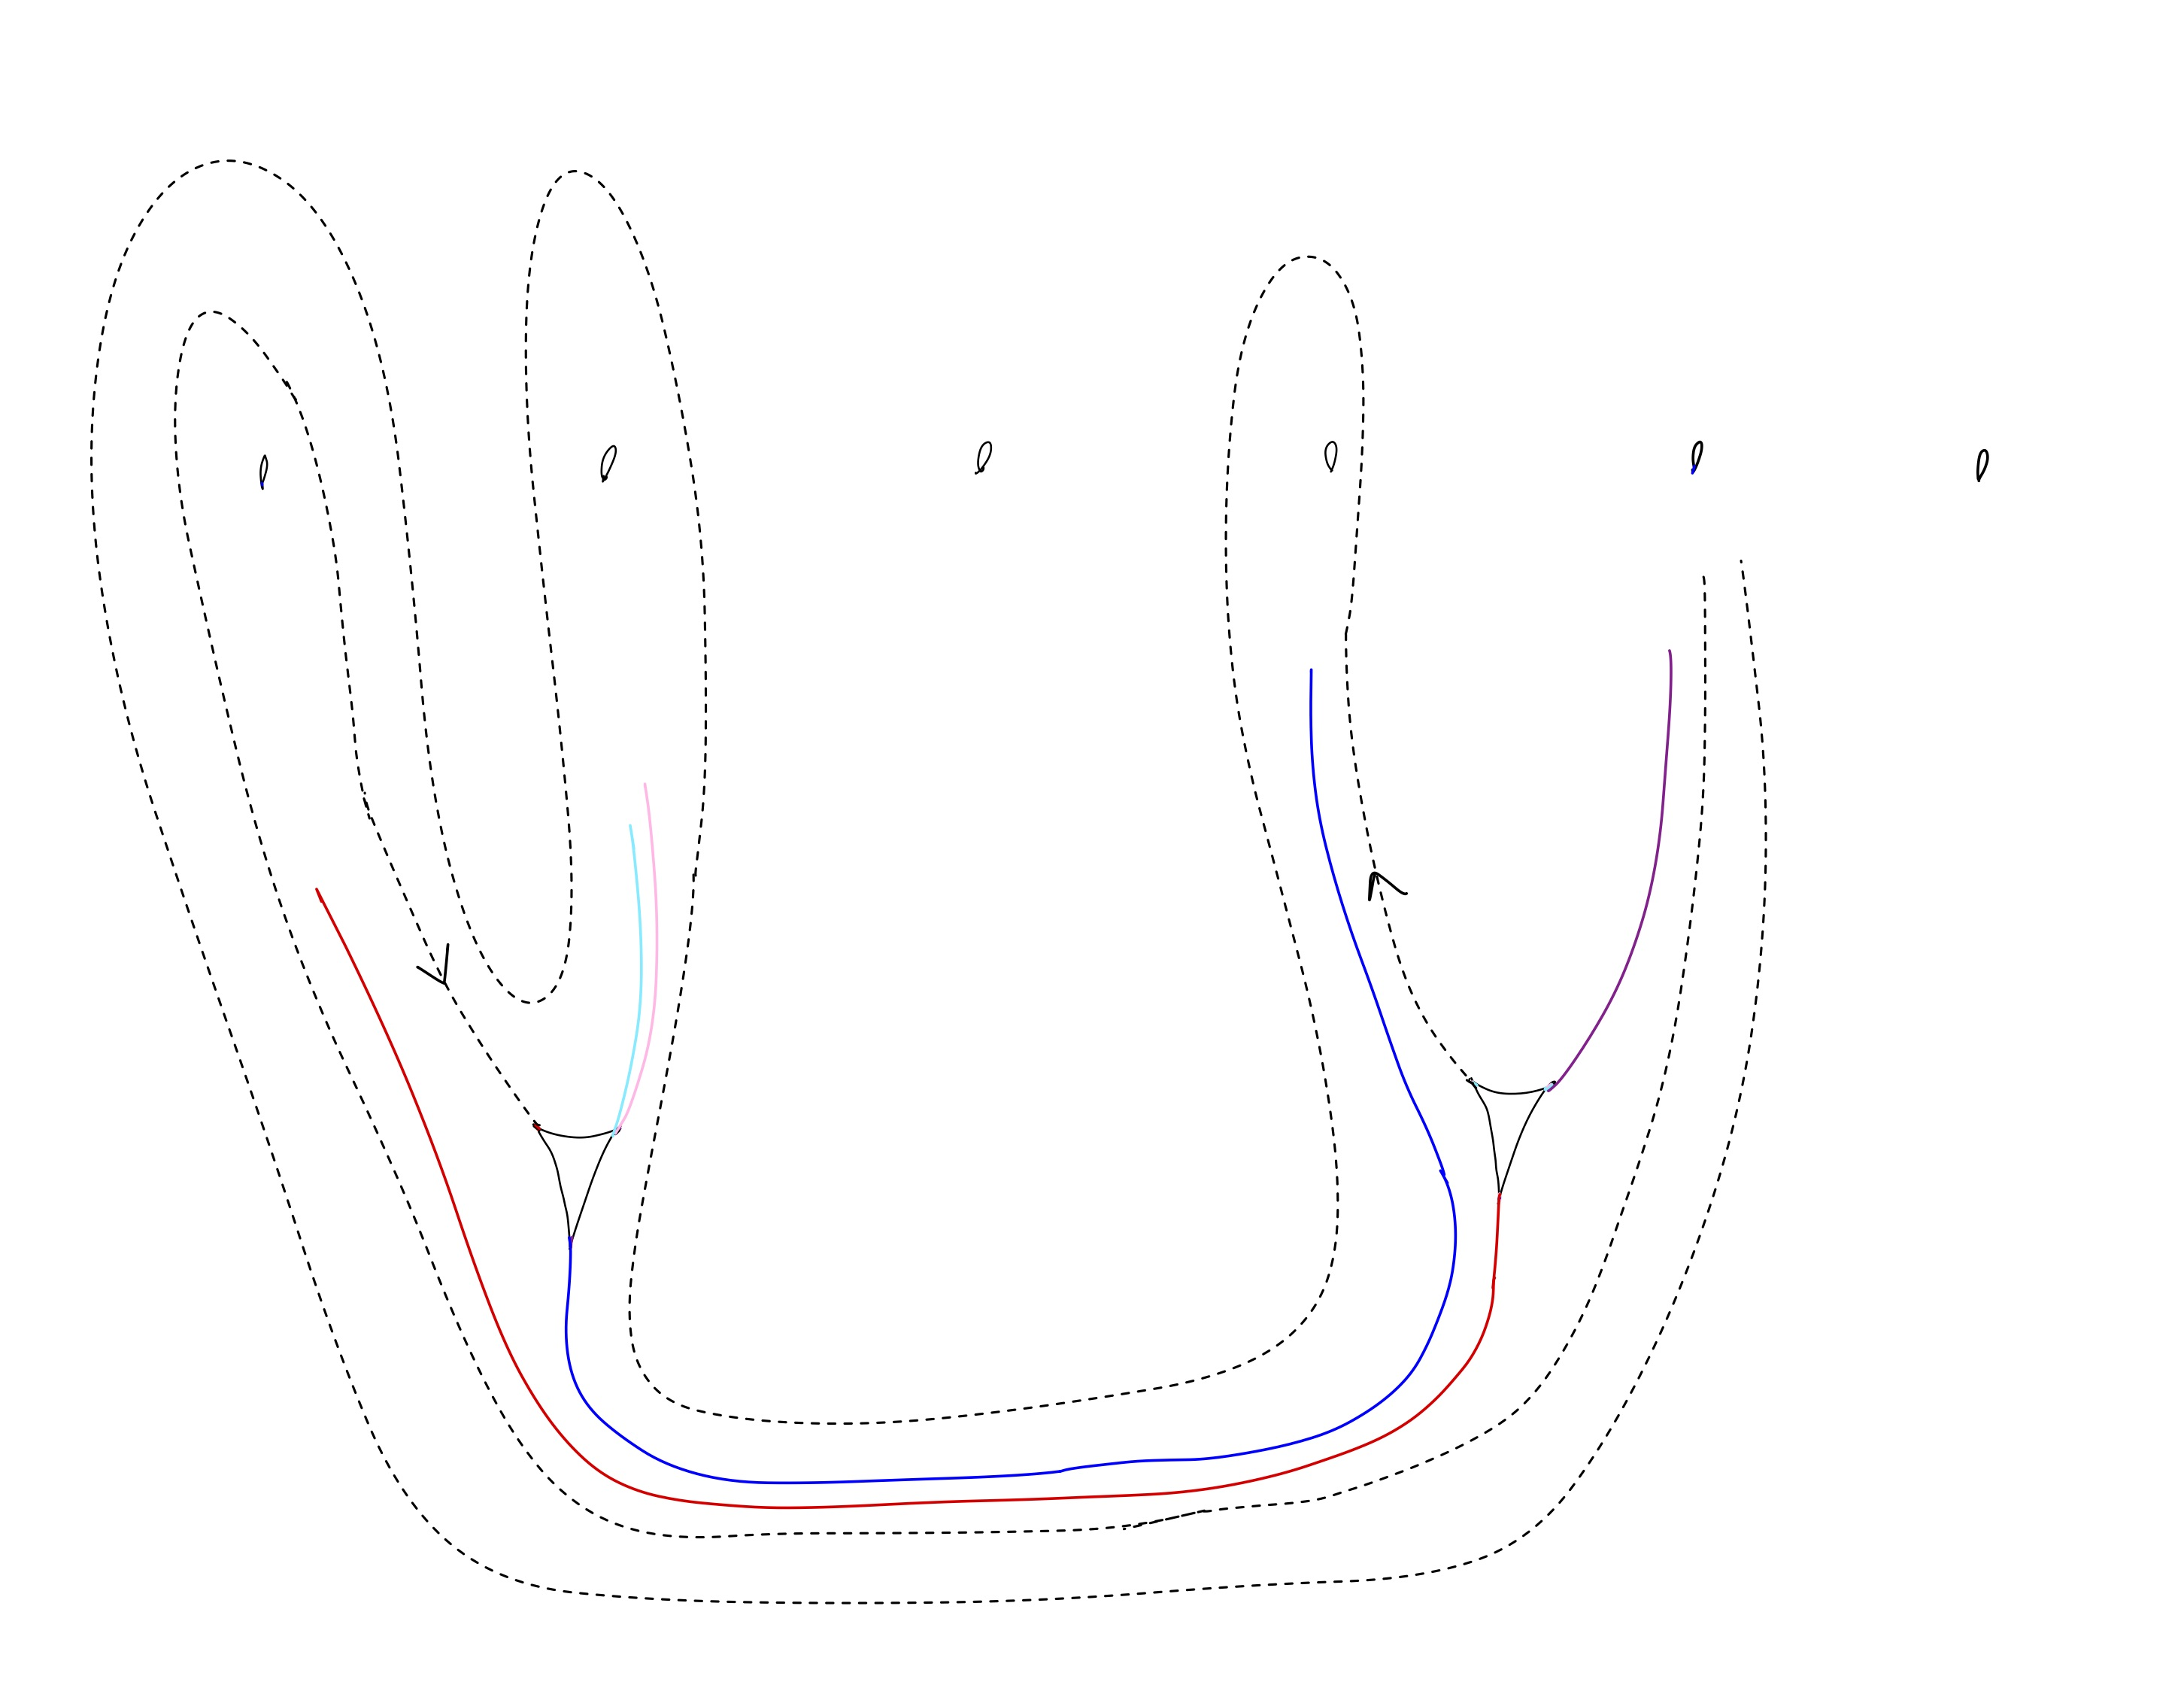
\includegraphics[width=\linewidth]{figures_case_analysis/track17_case_analysis/GBR-04.jpg}
    \caption{GBR4}
    \label{fig:GBR4}
\end{figure}

\begin{figure}[ht]
    \centering
    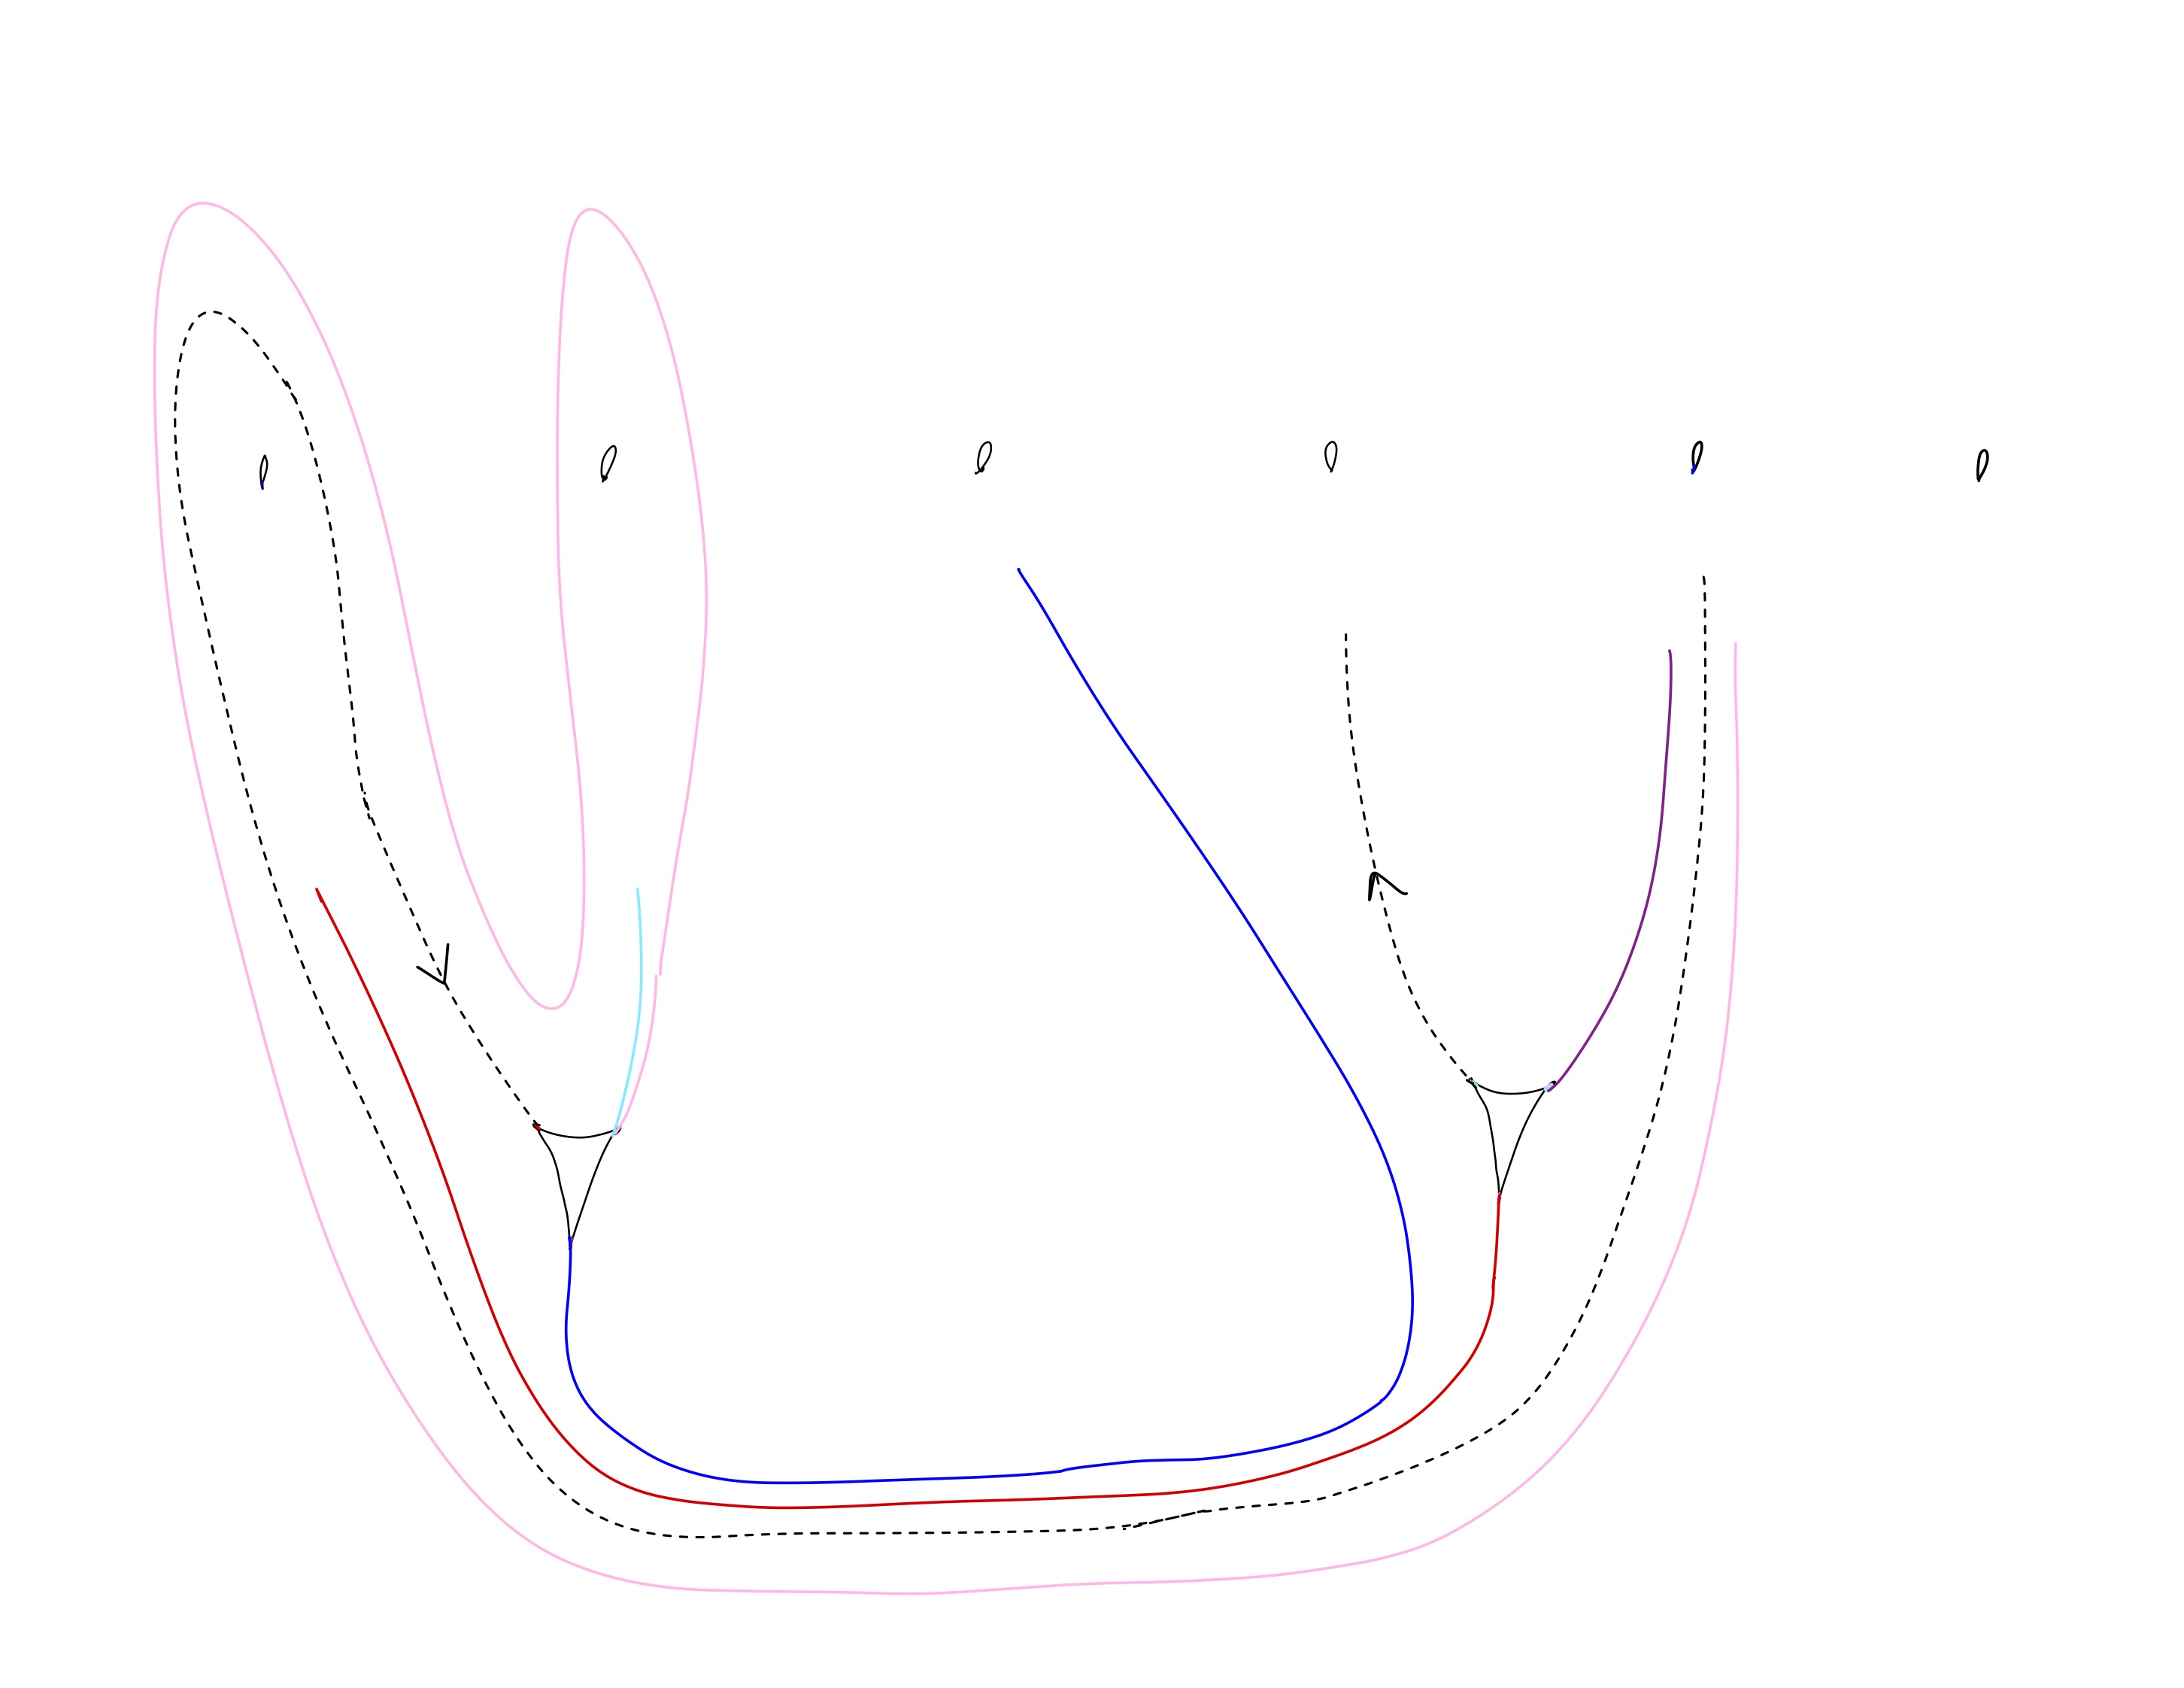
\includegraphics[width=\linewidth]{figures_case_analysis/track17_case_analysis/GBR-05.jpg}
    \caption{GBR5}
    \label{fig:GBR5}
\end{figure}

\begin{figure}[ht]
    \centering
    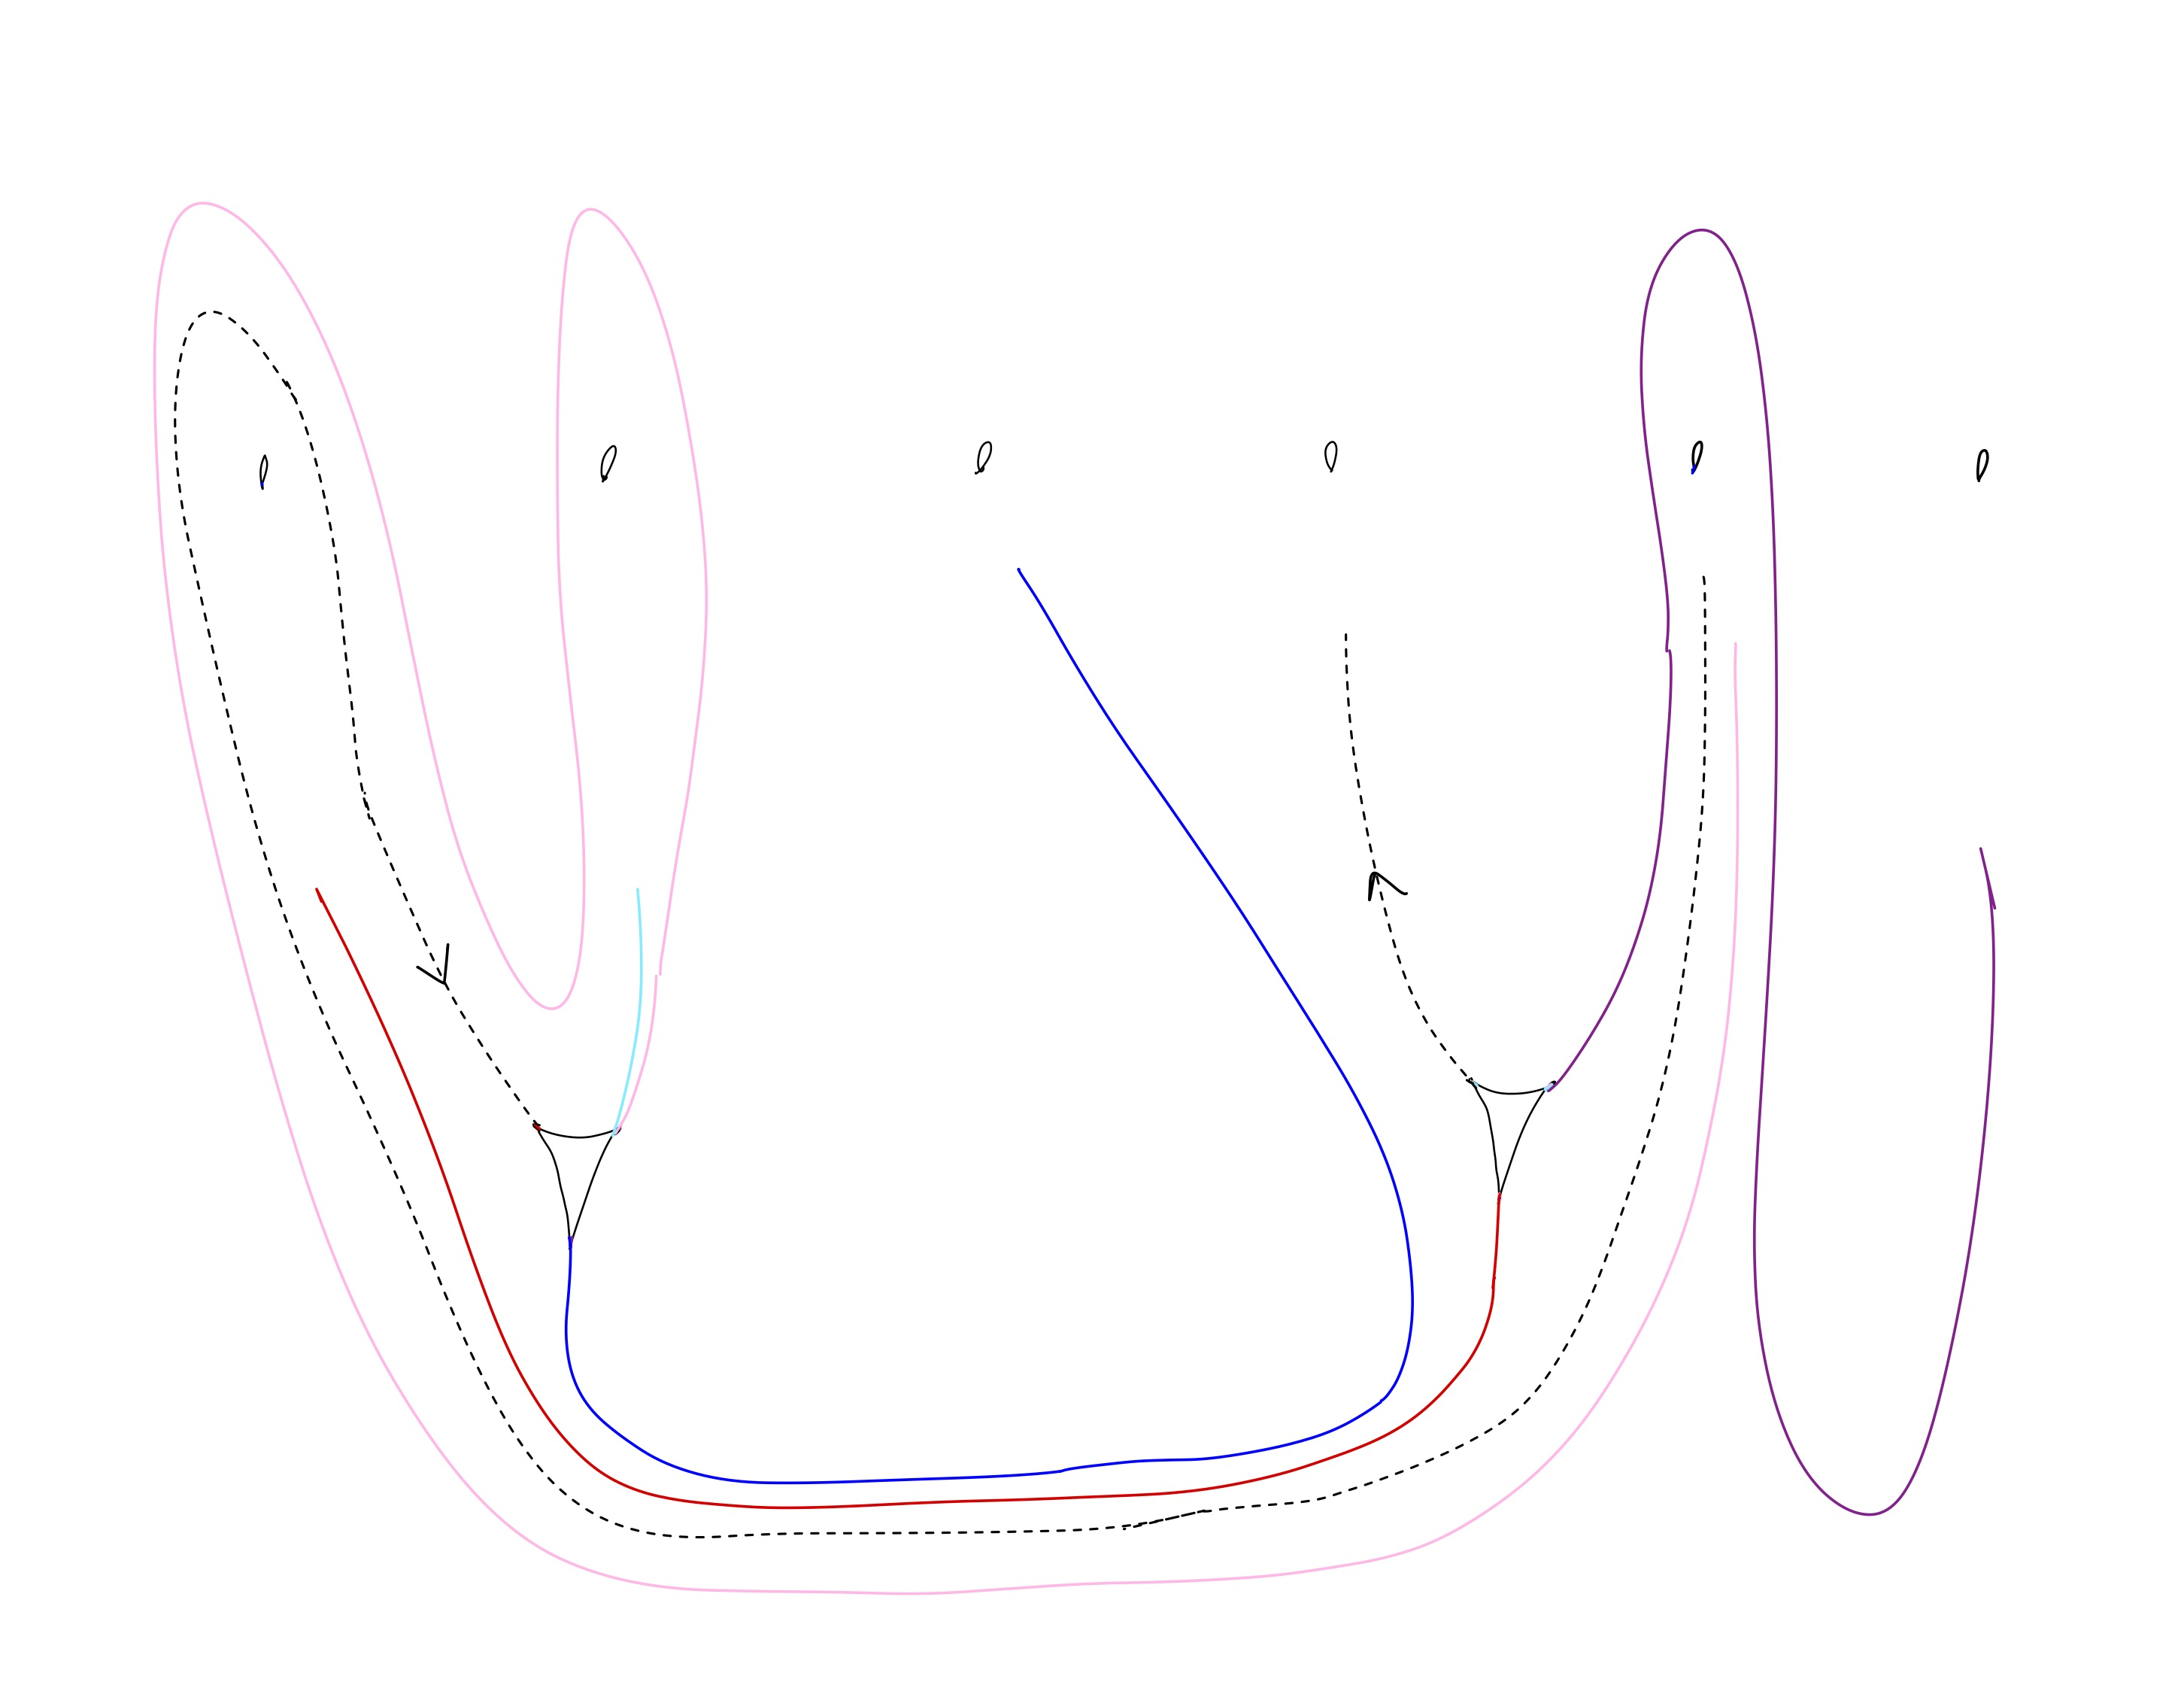
\includegraphics[width=\linewidth]{figures_case_analysis/track17_case_analysis/GBR-06.jpg}
    \caption{GBR6}
    \label{fig:GBR6}
\end{figure}

\begin{figure}[ht]
    \centering
    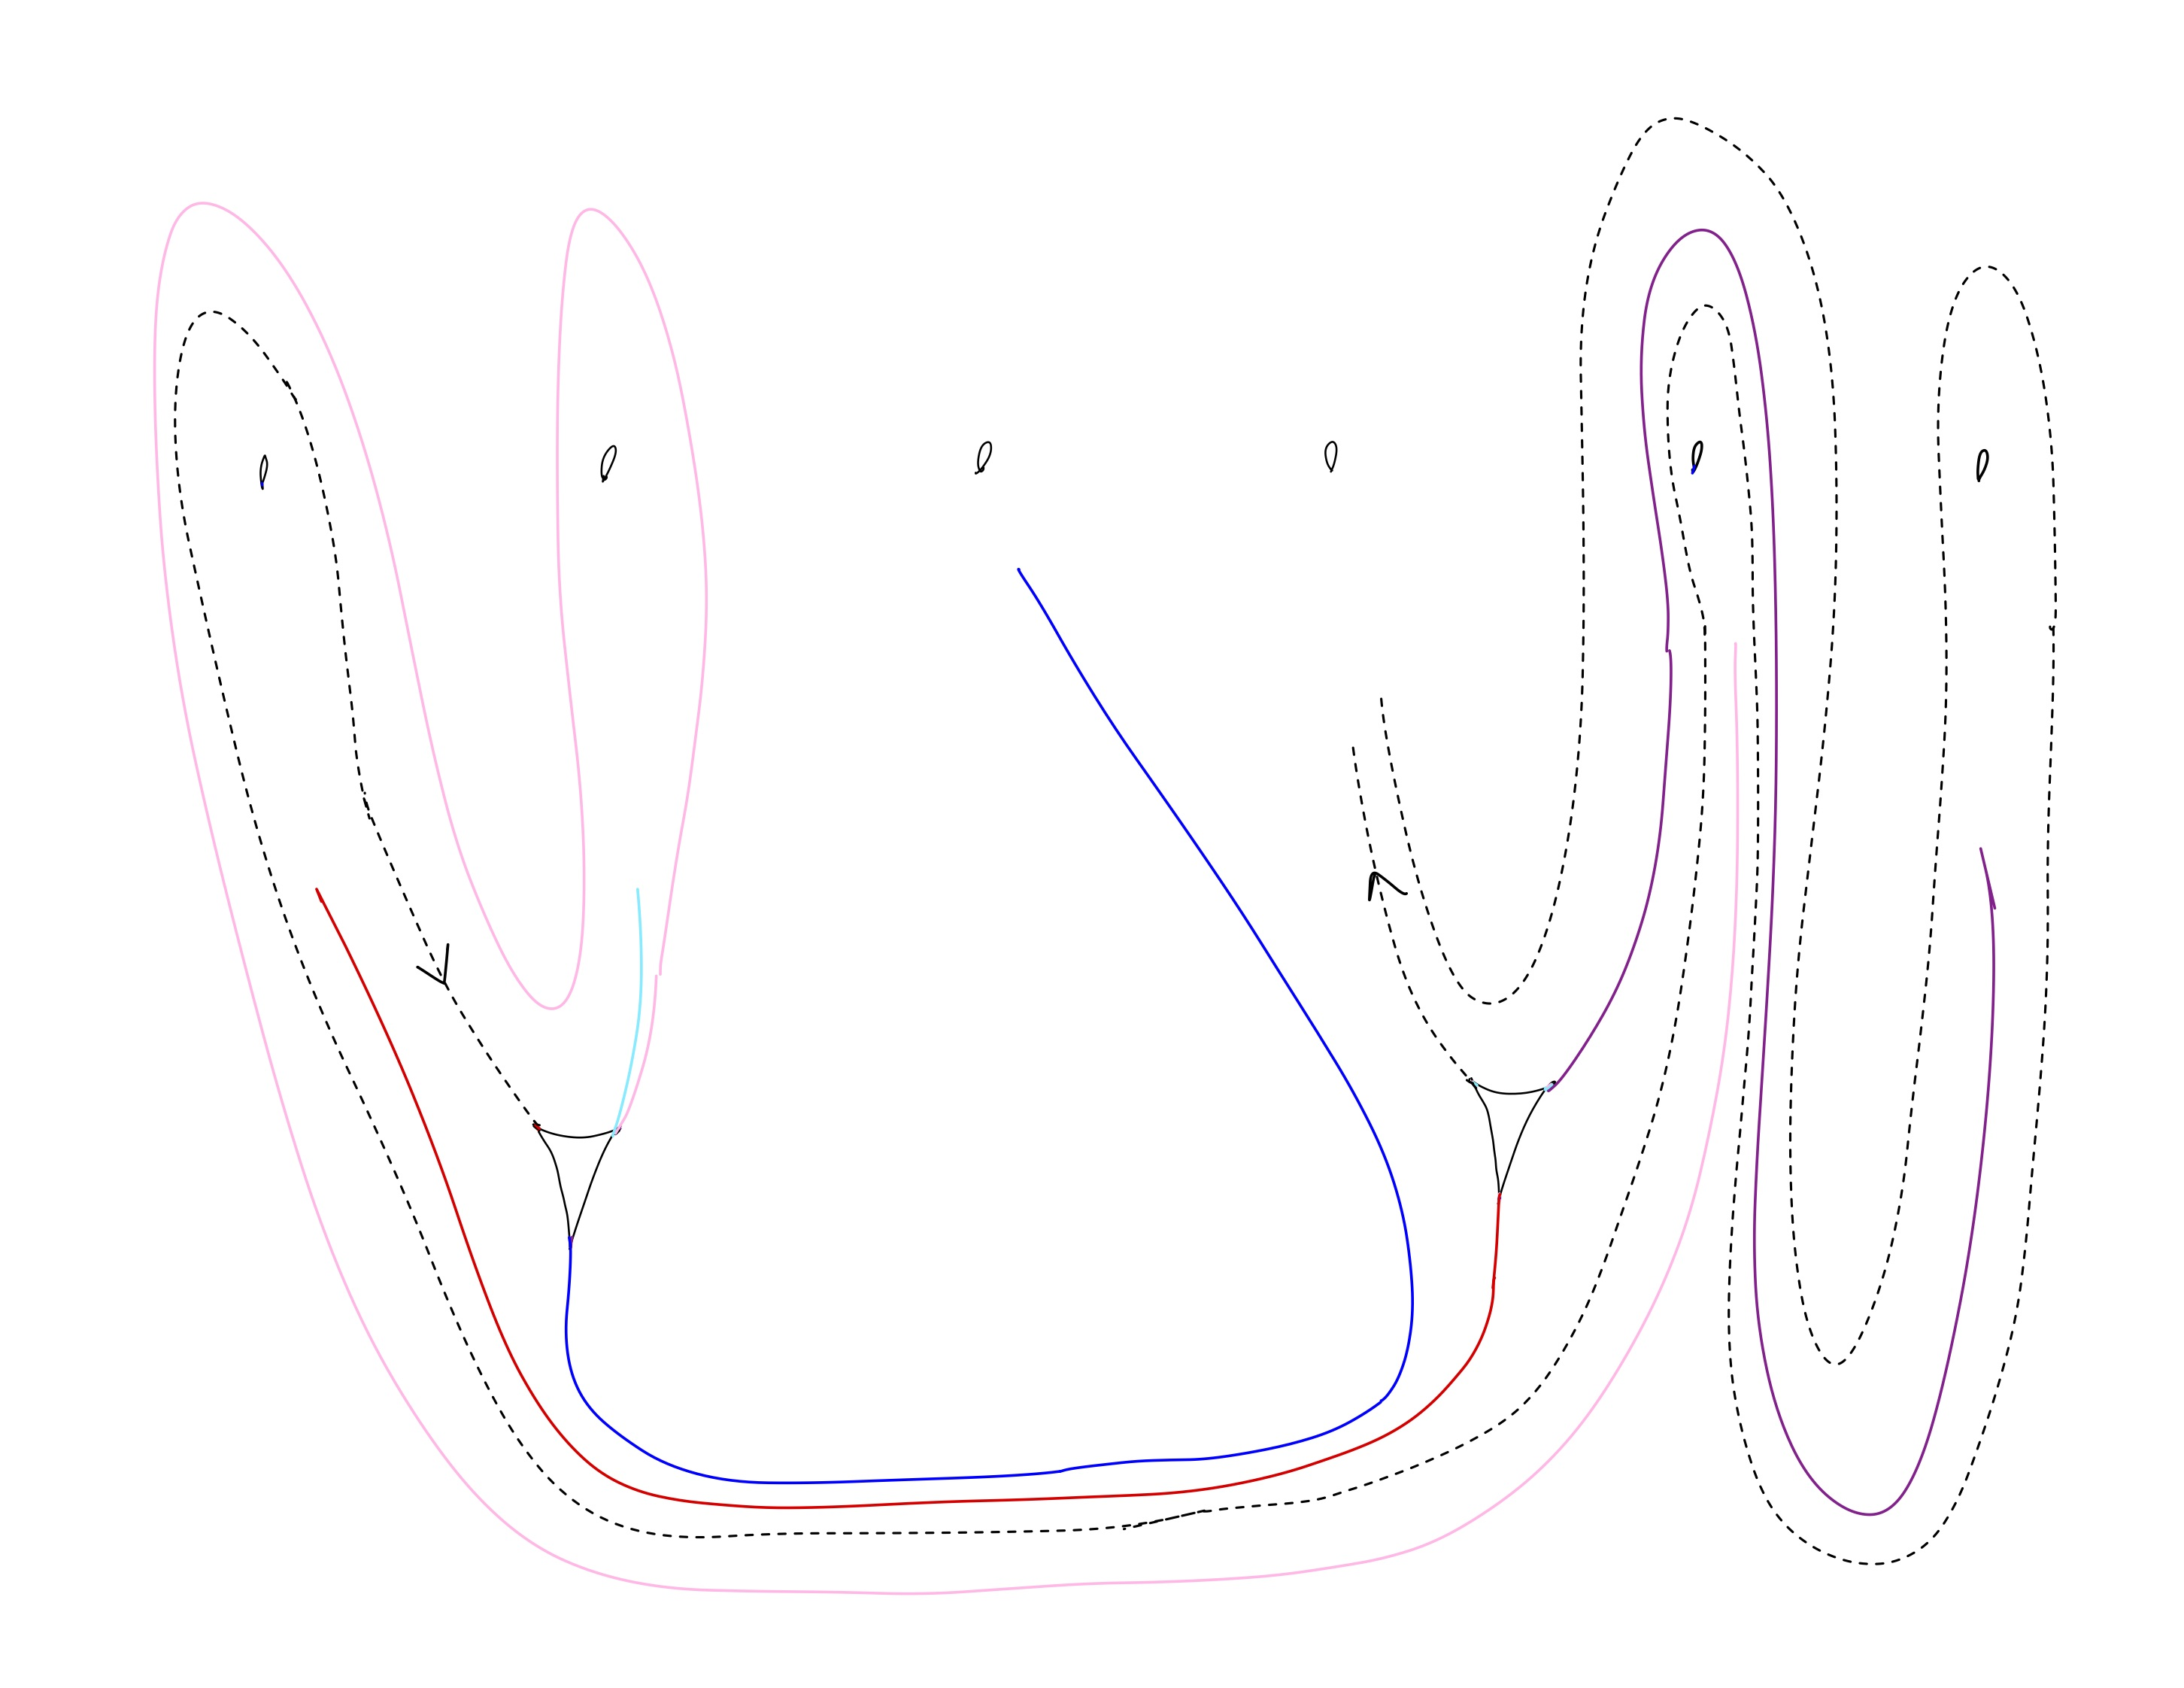
\includegraphics[width=\linewidth]{figures_case_analysis/track17_case_analysis/GBR-07.jpg}
    \caption{GBR7}
    \label{fig:GBR7}
\end{figure}

\begin{figure}[ht]
    \centering
    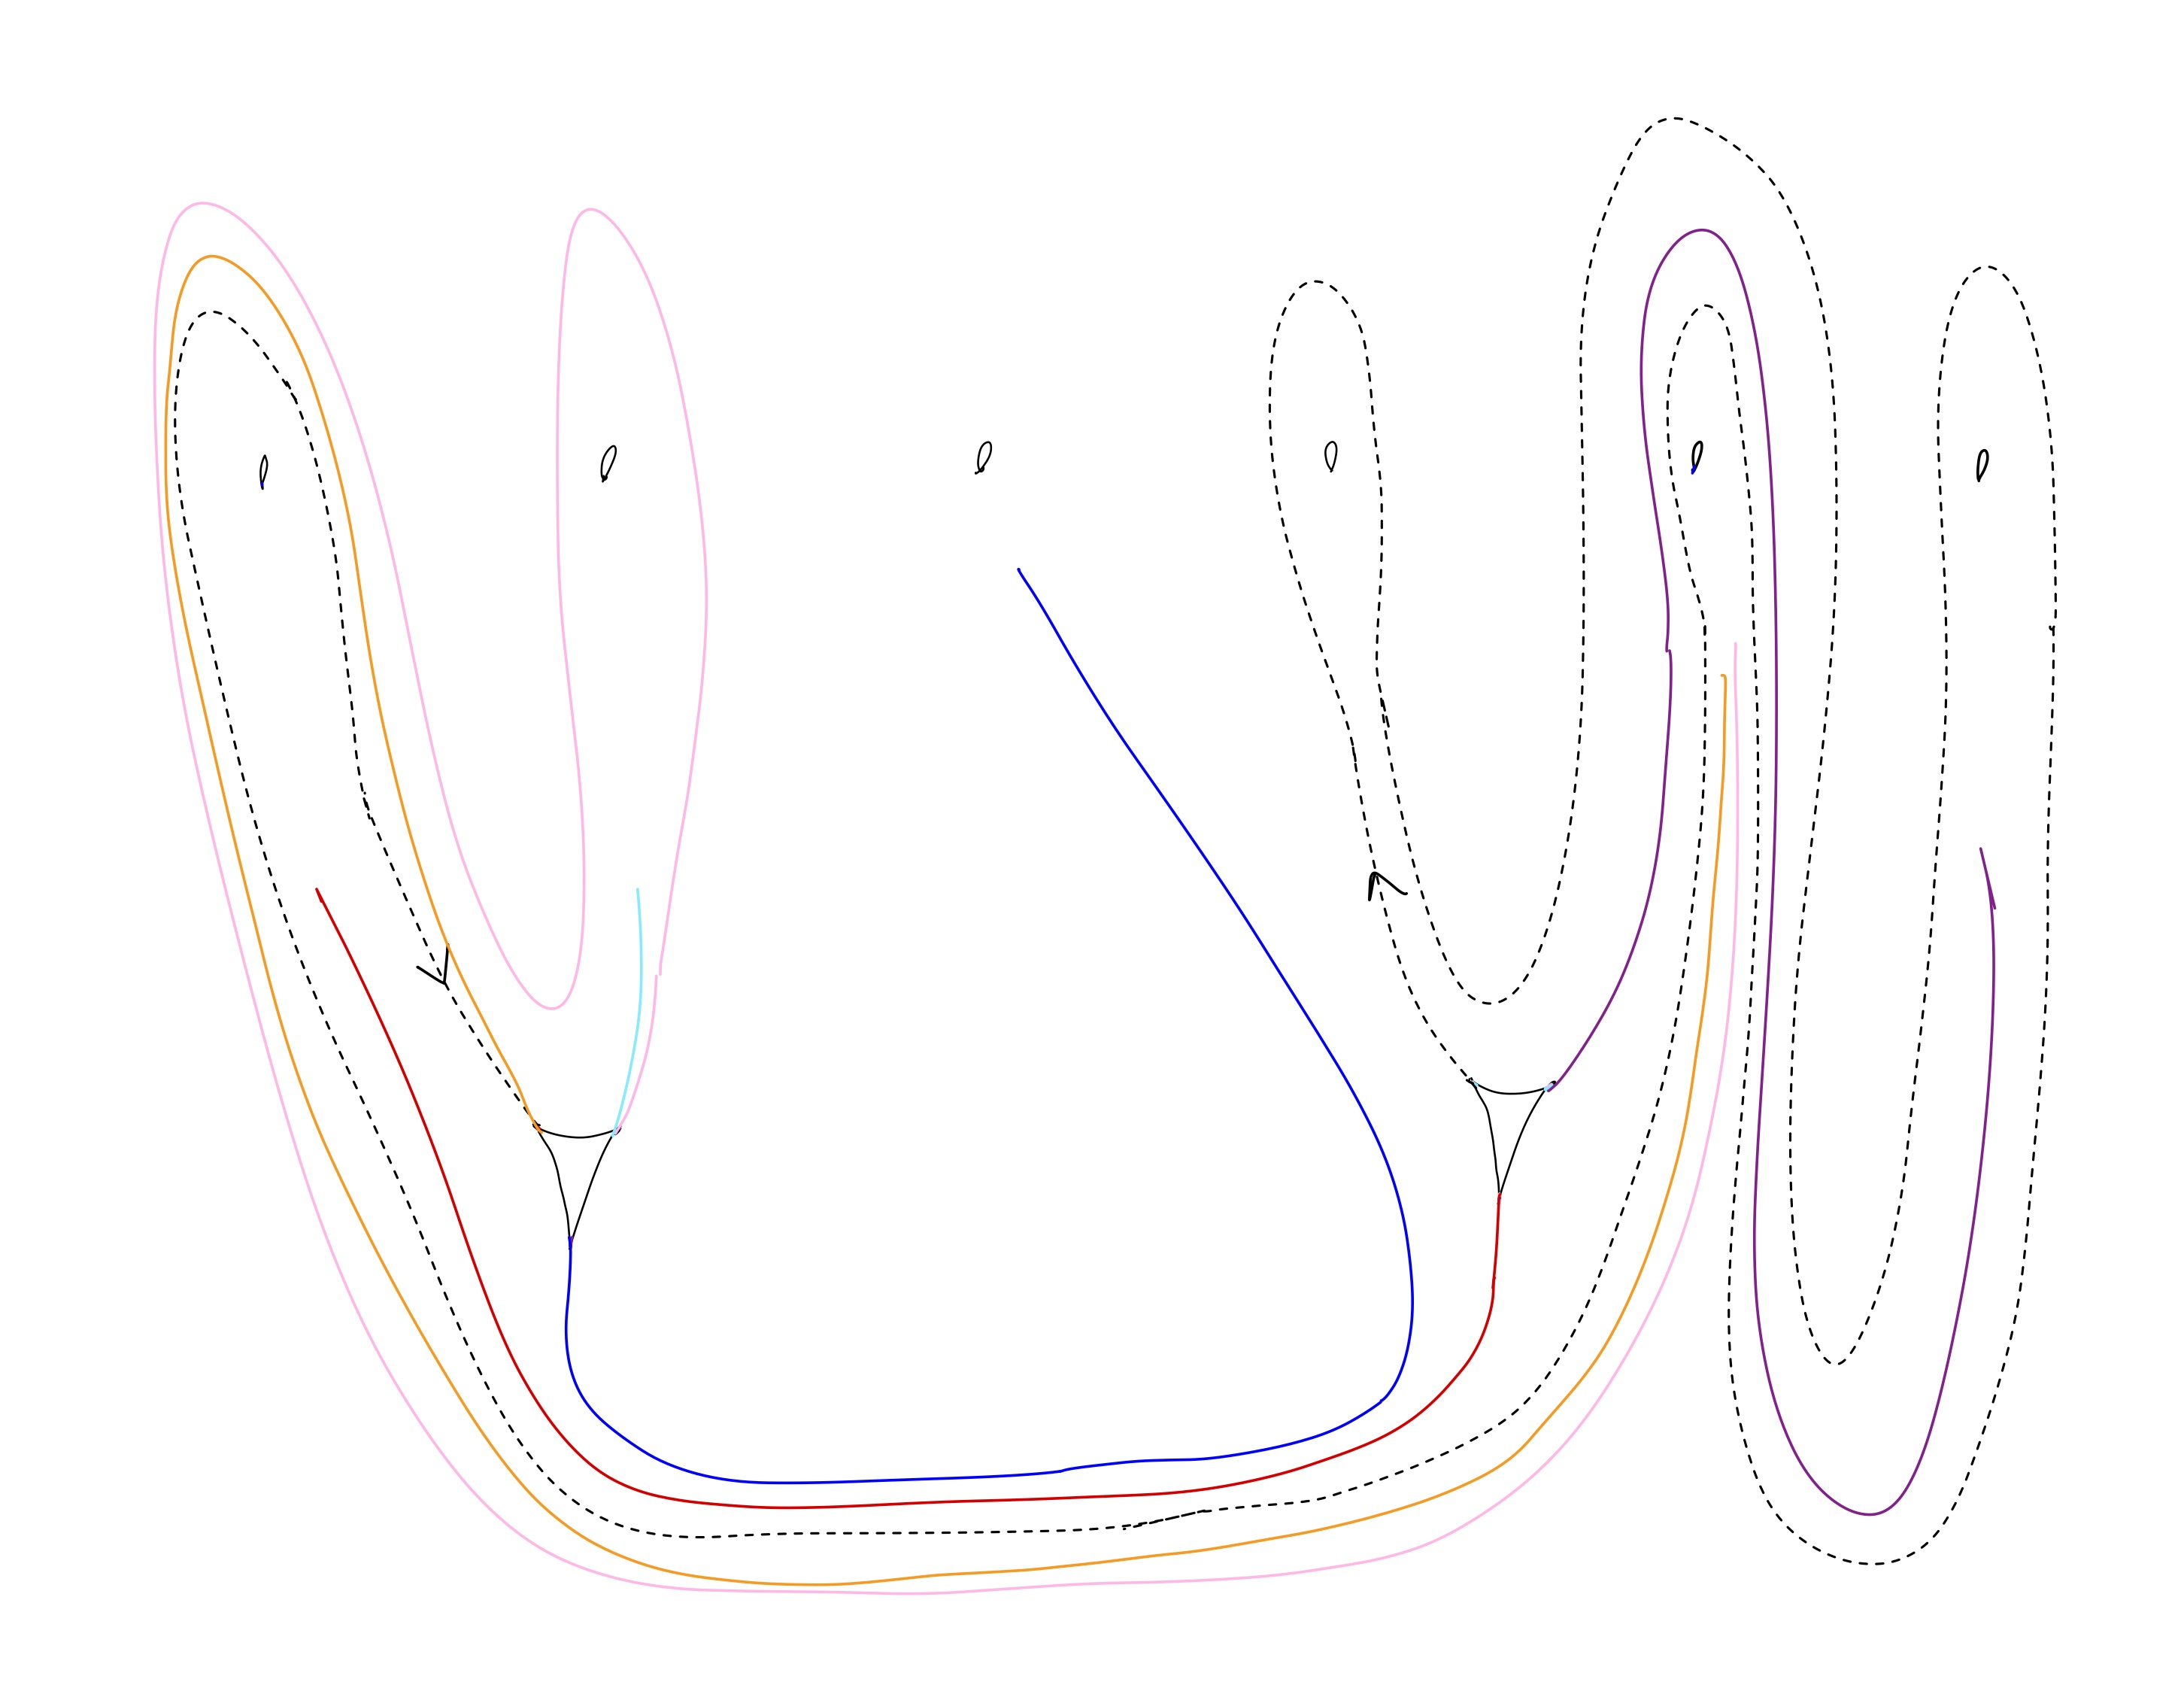
\includegraphics[width=\linewidth]{figures_case_analysis/track17_case_analysis/GBR-08.jpg}
    \caption{GBR8}
    \label{fig:GBR8}
\end{figure}

\begin{figure}[ht]
    \centering
    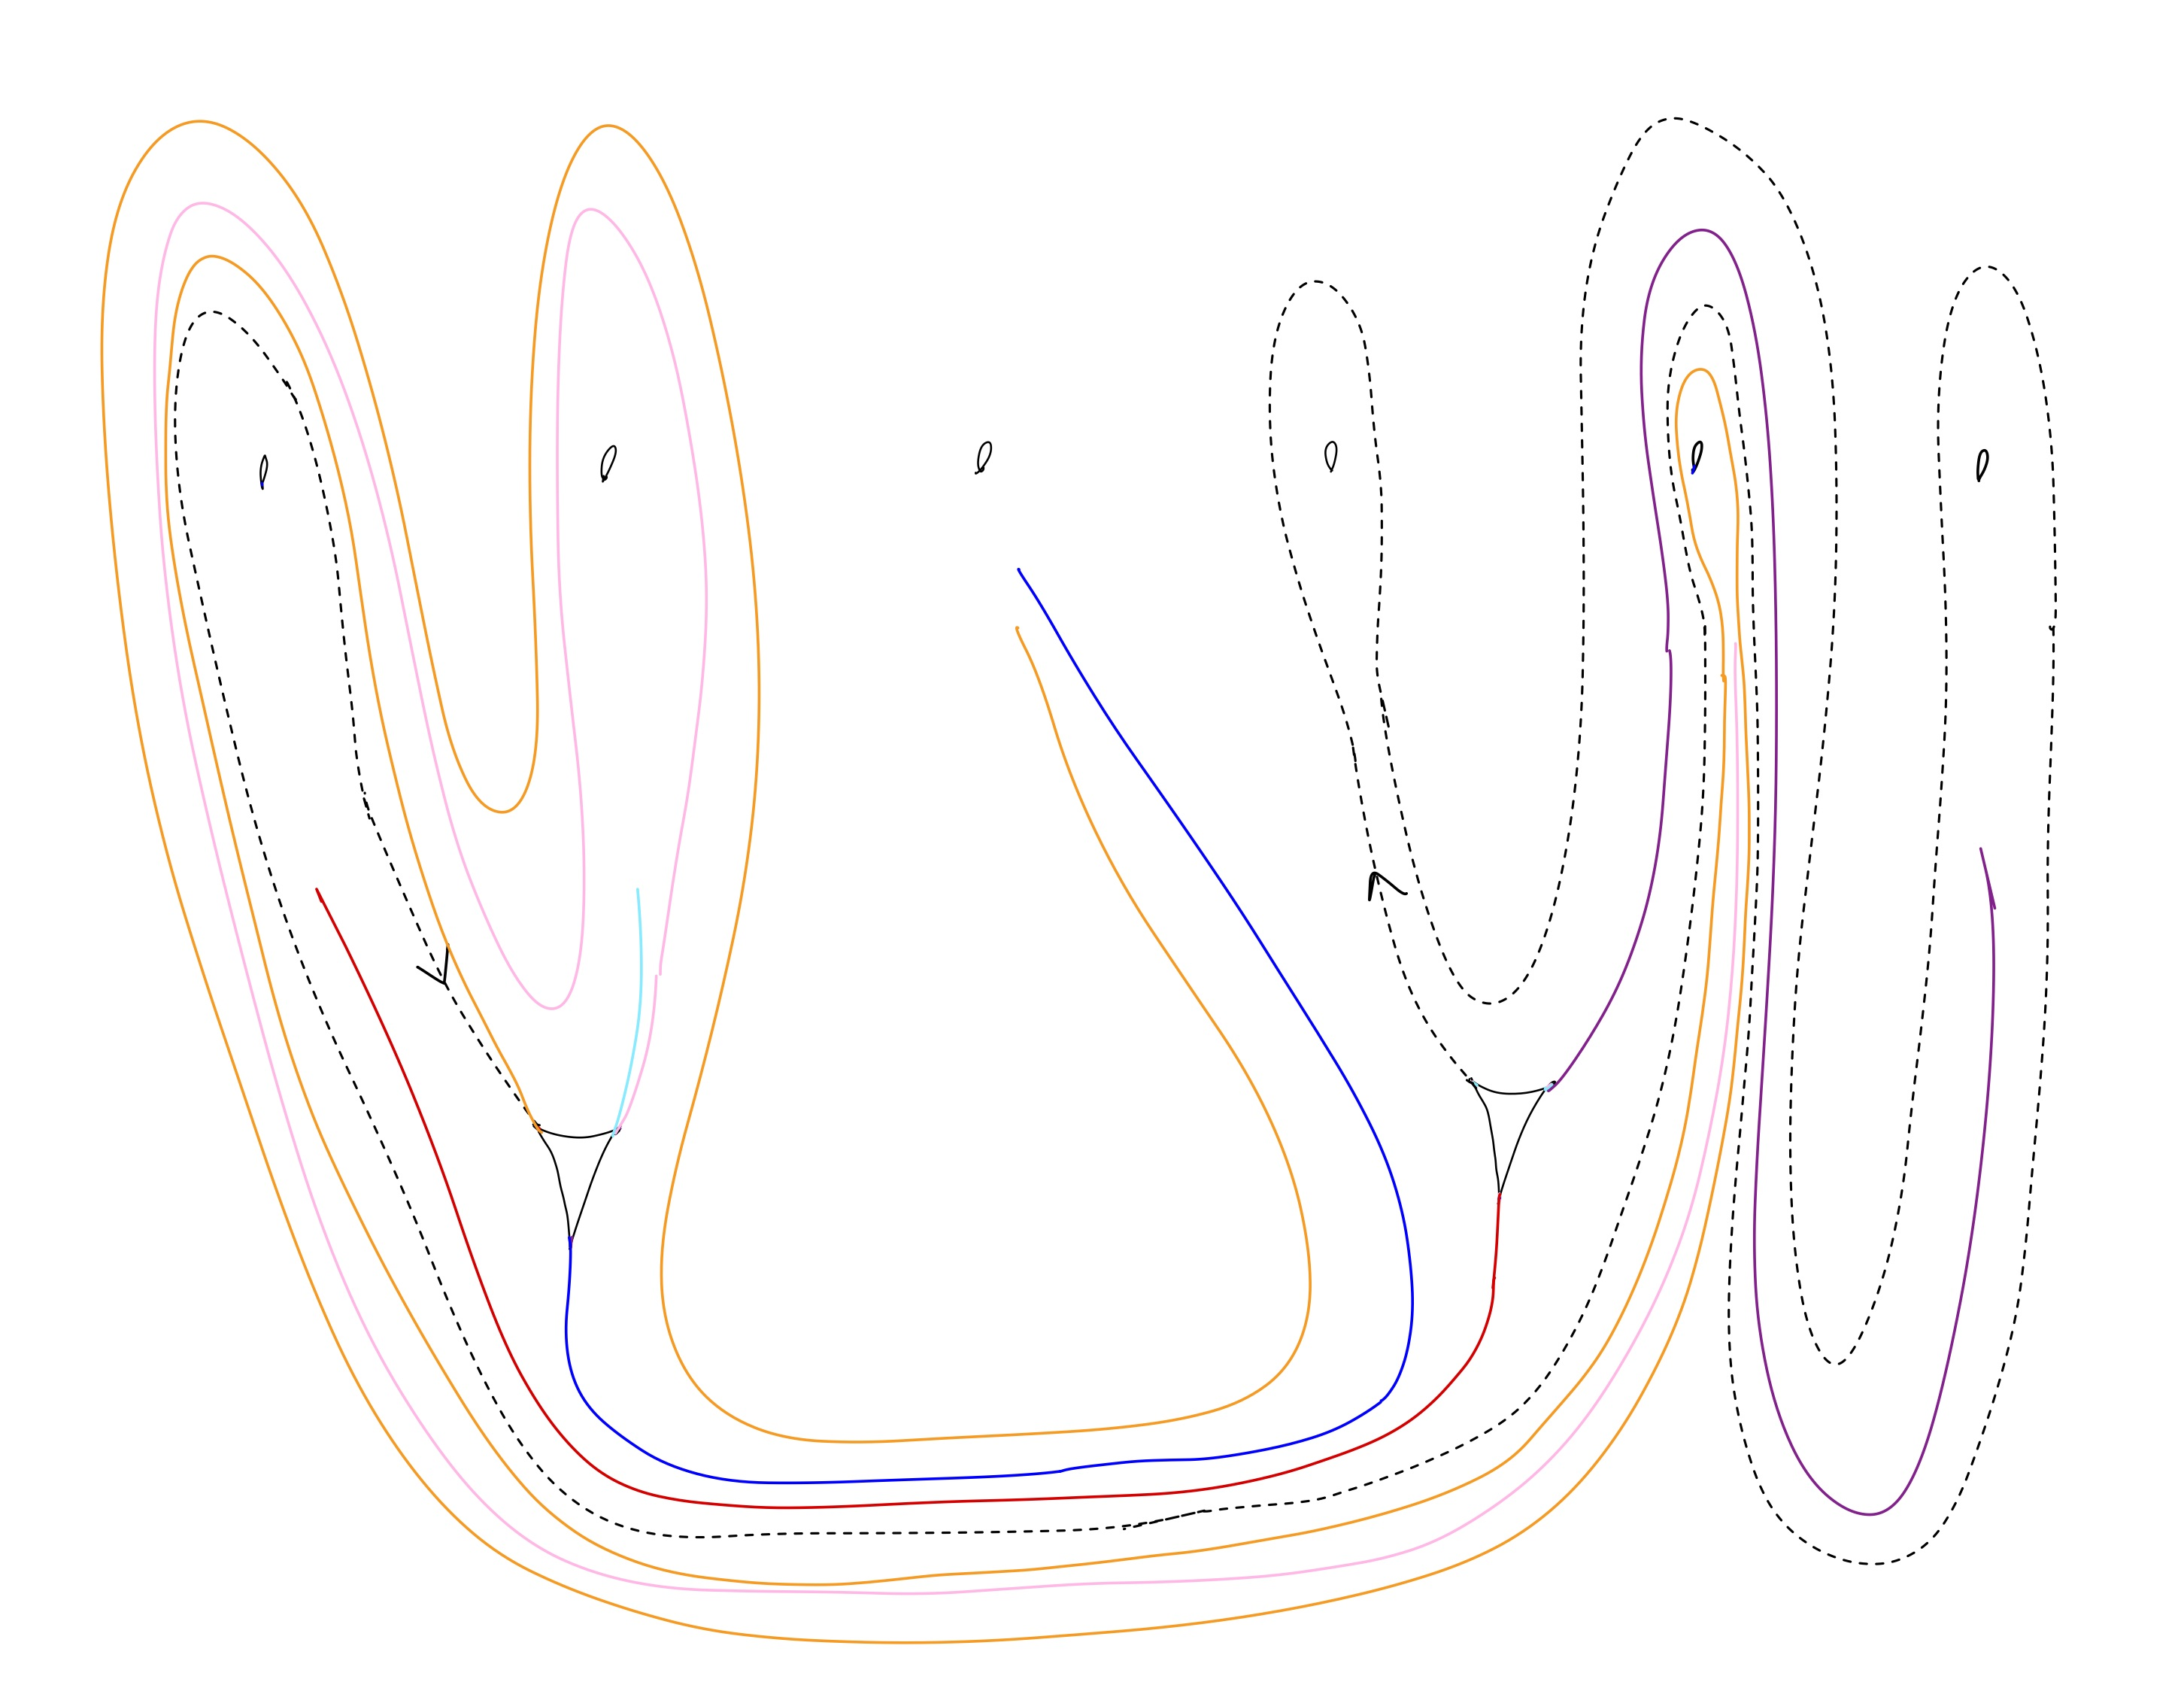
\includegraphics[width=\linewidth]{figures_case_analysis/track17_case_analysis/GBR-09.jpg}
    \caption{GBR9}
    \label{fig:GBR9}
\end{figure}

\begin{figure}[ht]
    \centering
    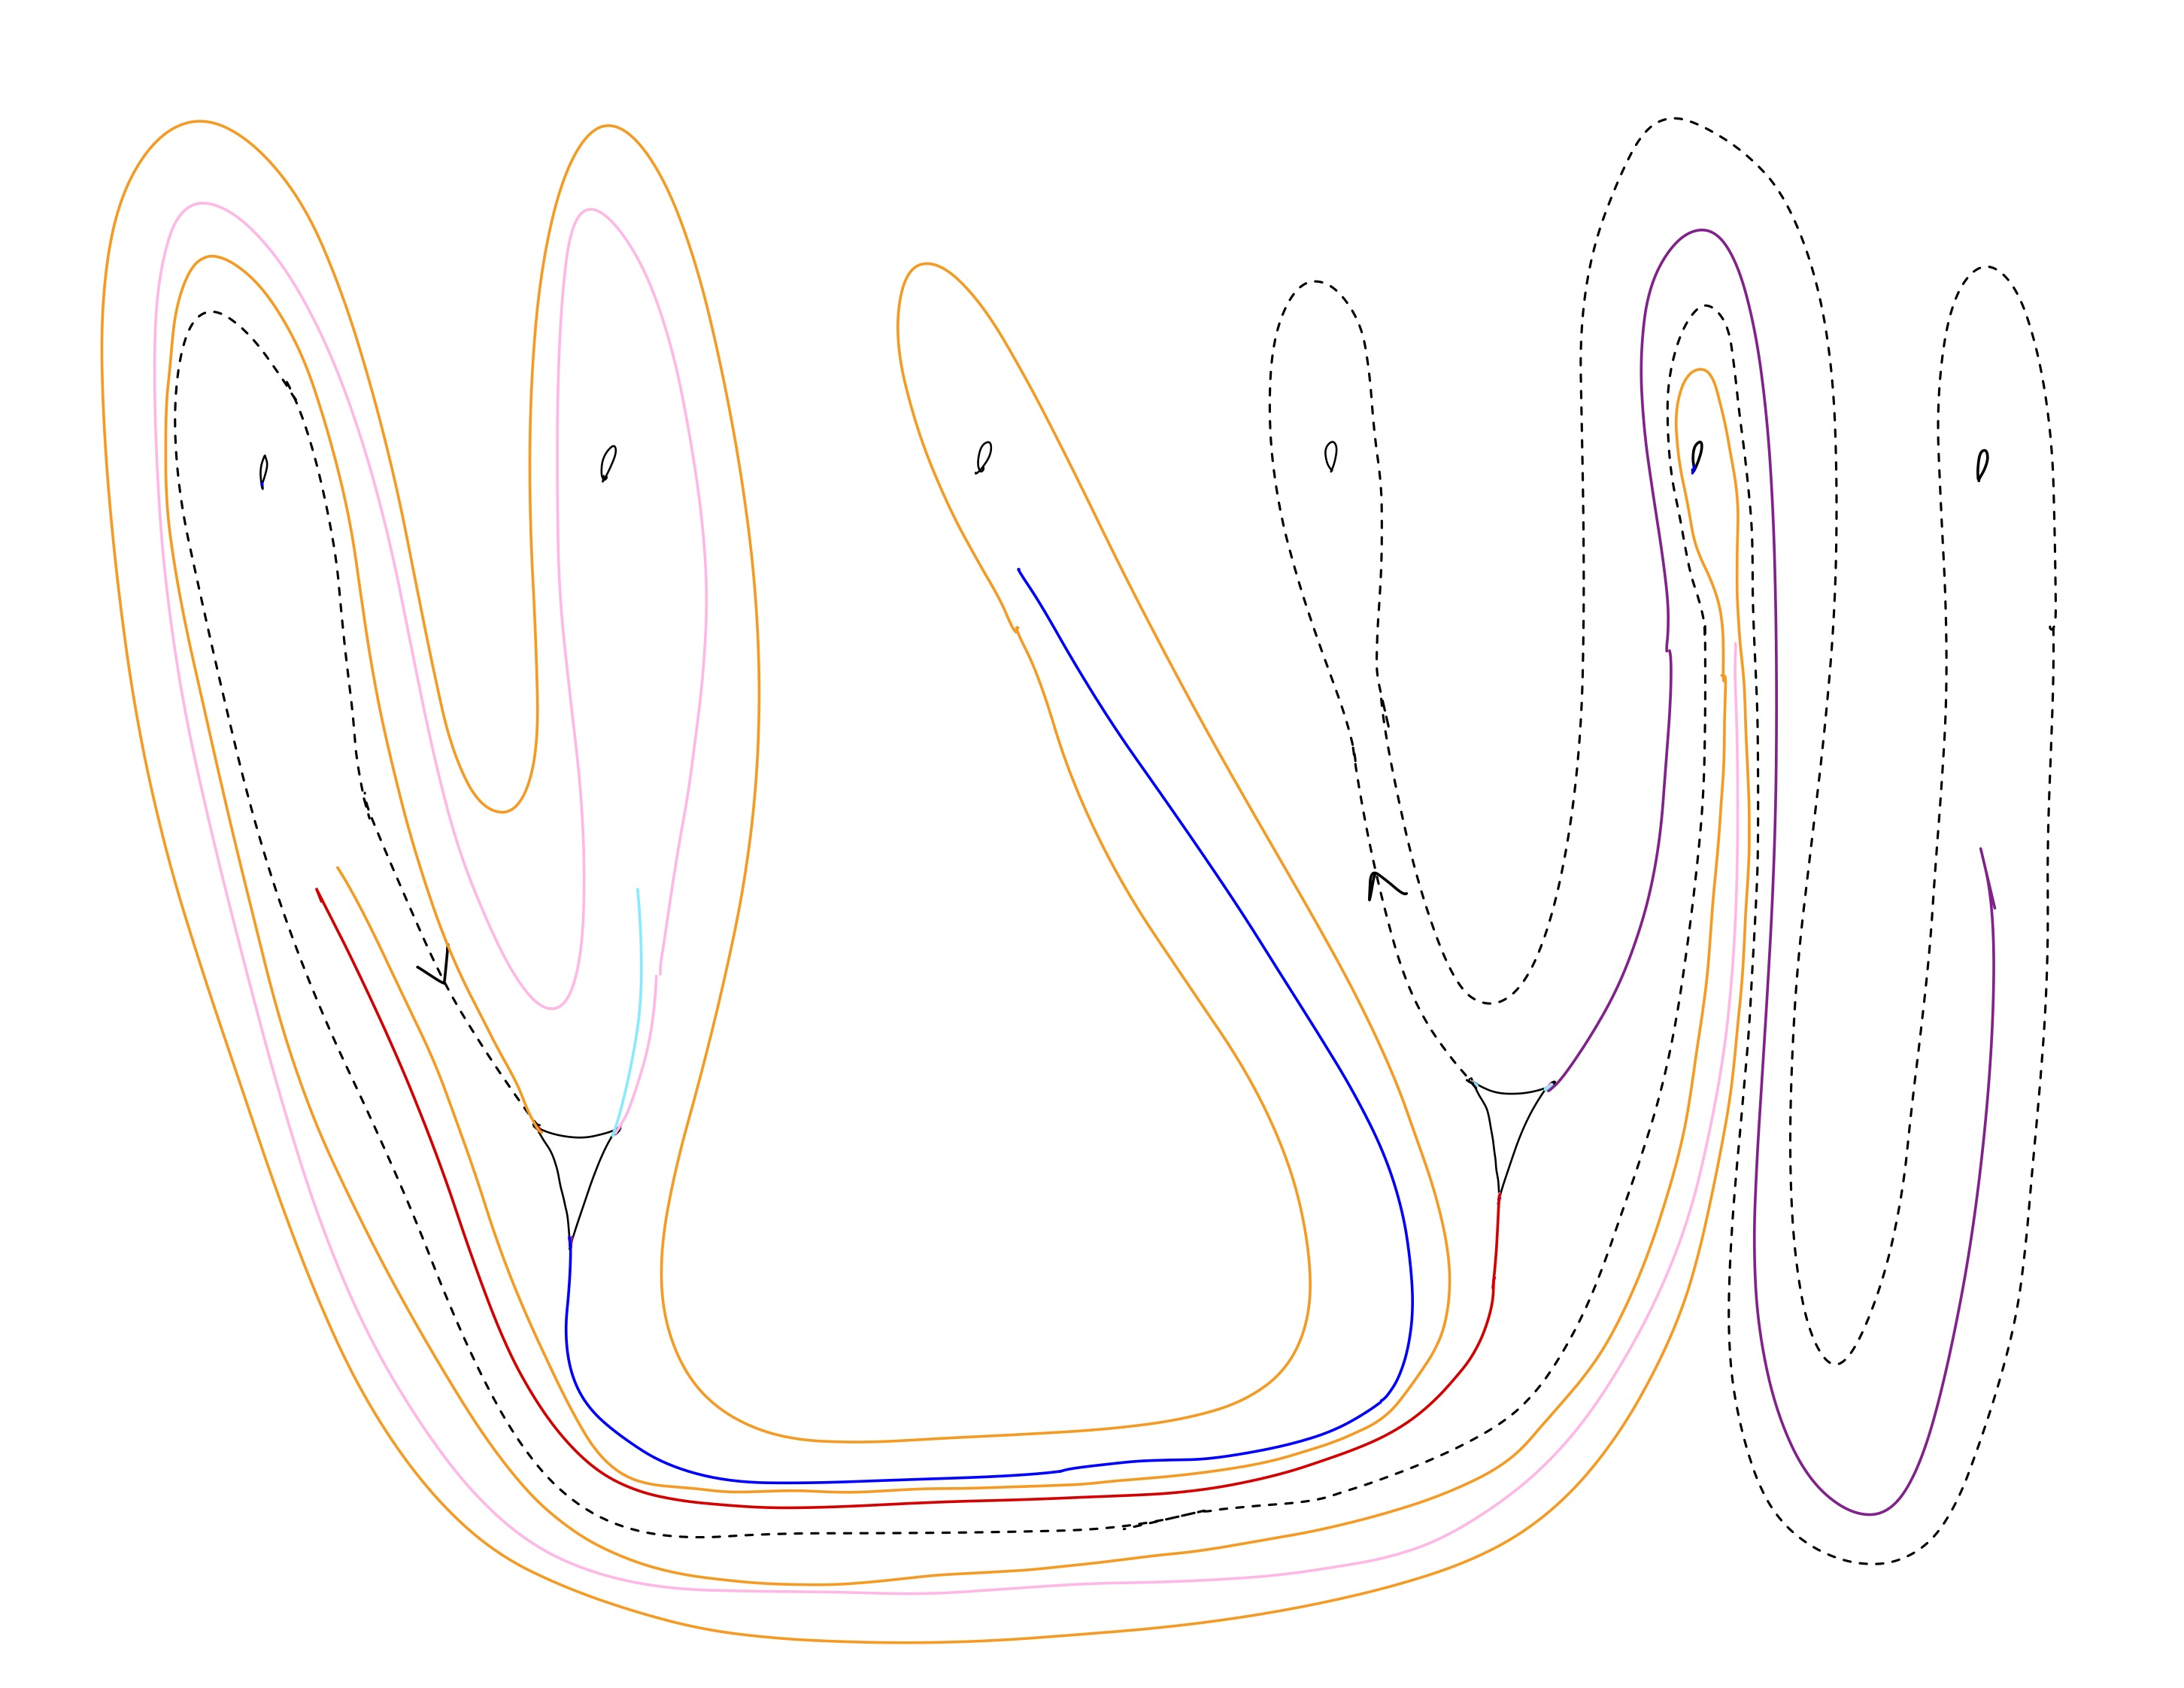
\includegraphics[width=\linewidth]{figures_case_analysis/track17_case_analysis/GBR-10.jpg}
    \caption{GBR10}
    \label{fig:GBR10}
\end{figure}

\begin{figure}[ht]
    \centering
    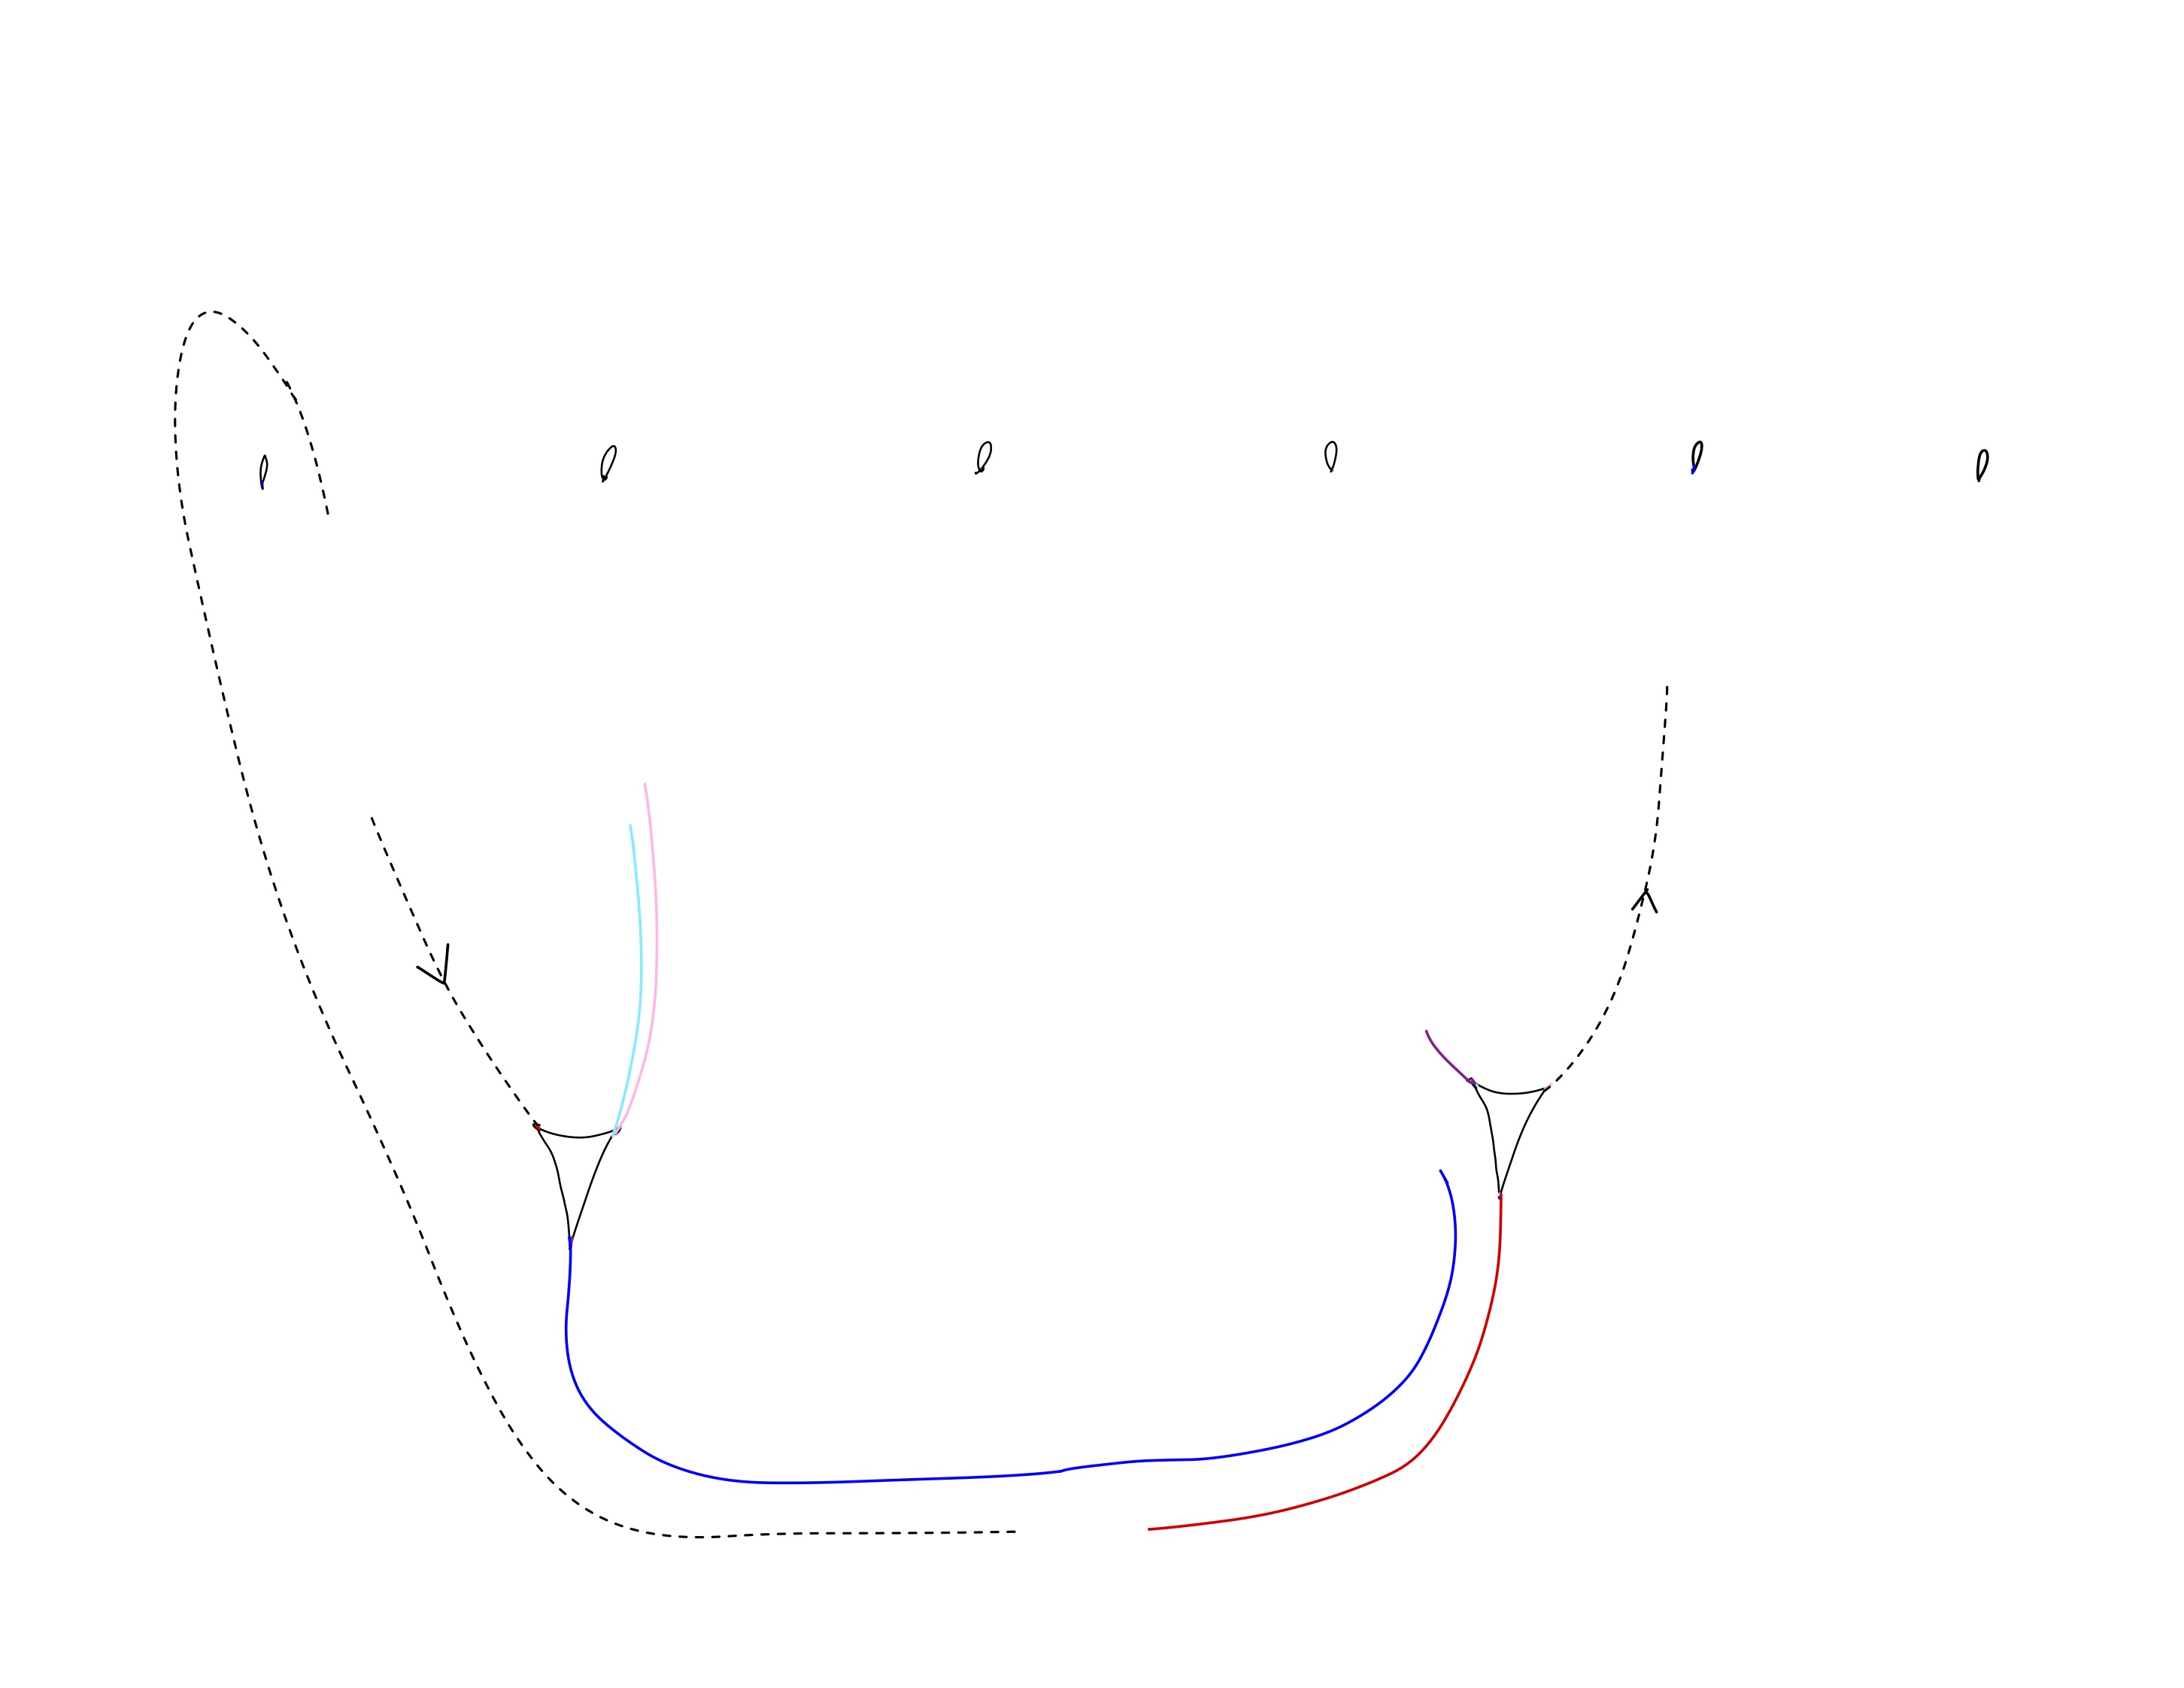
\includegraphics[width=\linewidth]{figures_case_analysis/track17_case_analysis/GBR-11.jpg}
    \caption{GBR11}
    \label{fig:GBR11}
\end{figure}

\begin{figure}[ht]
    \centering
    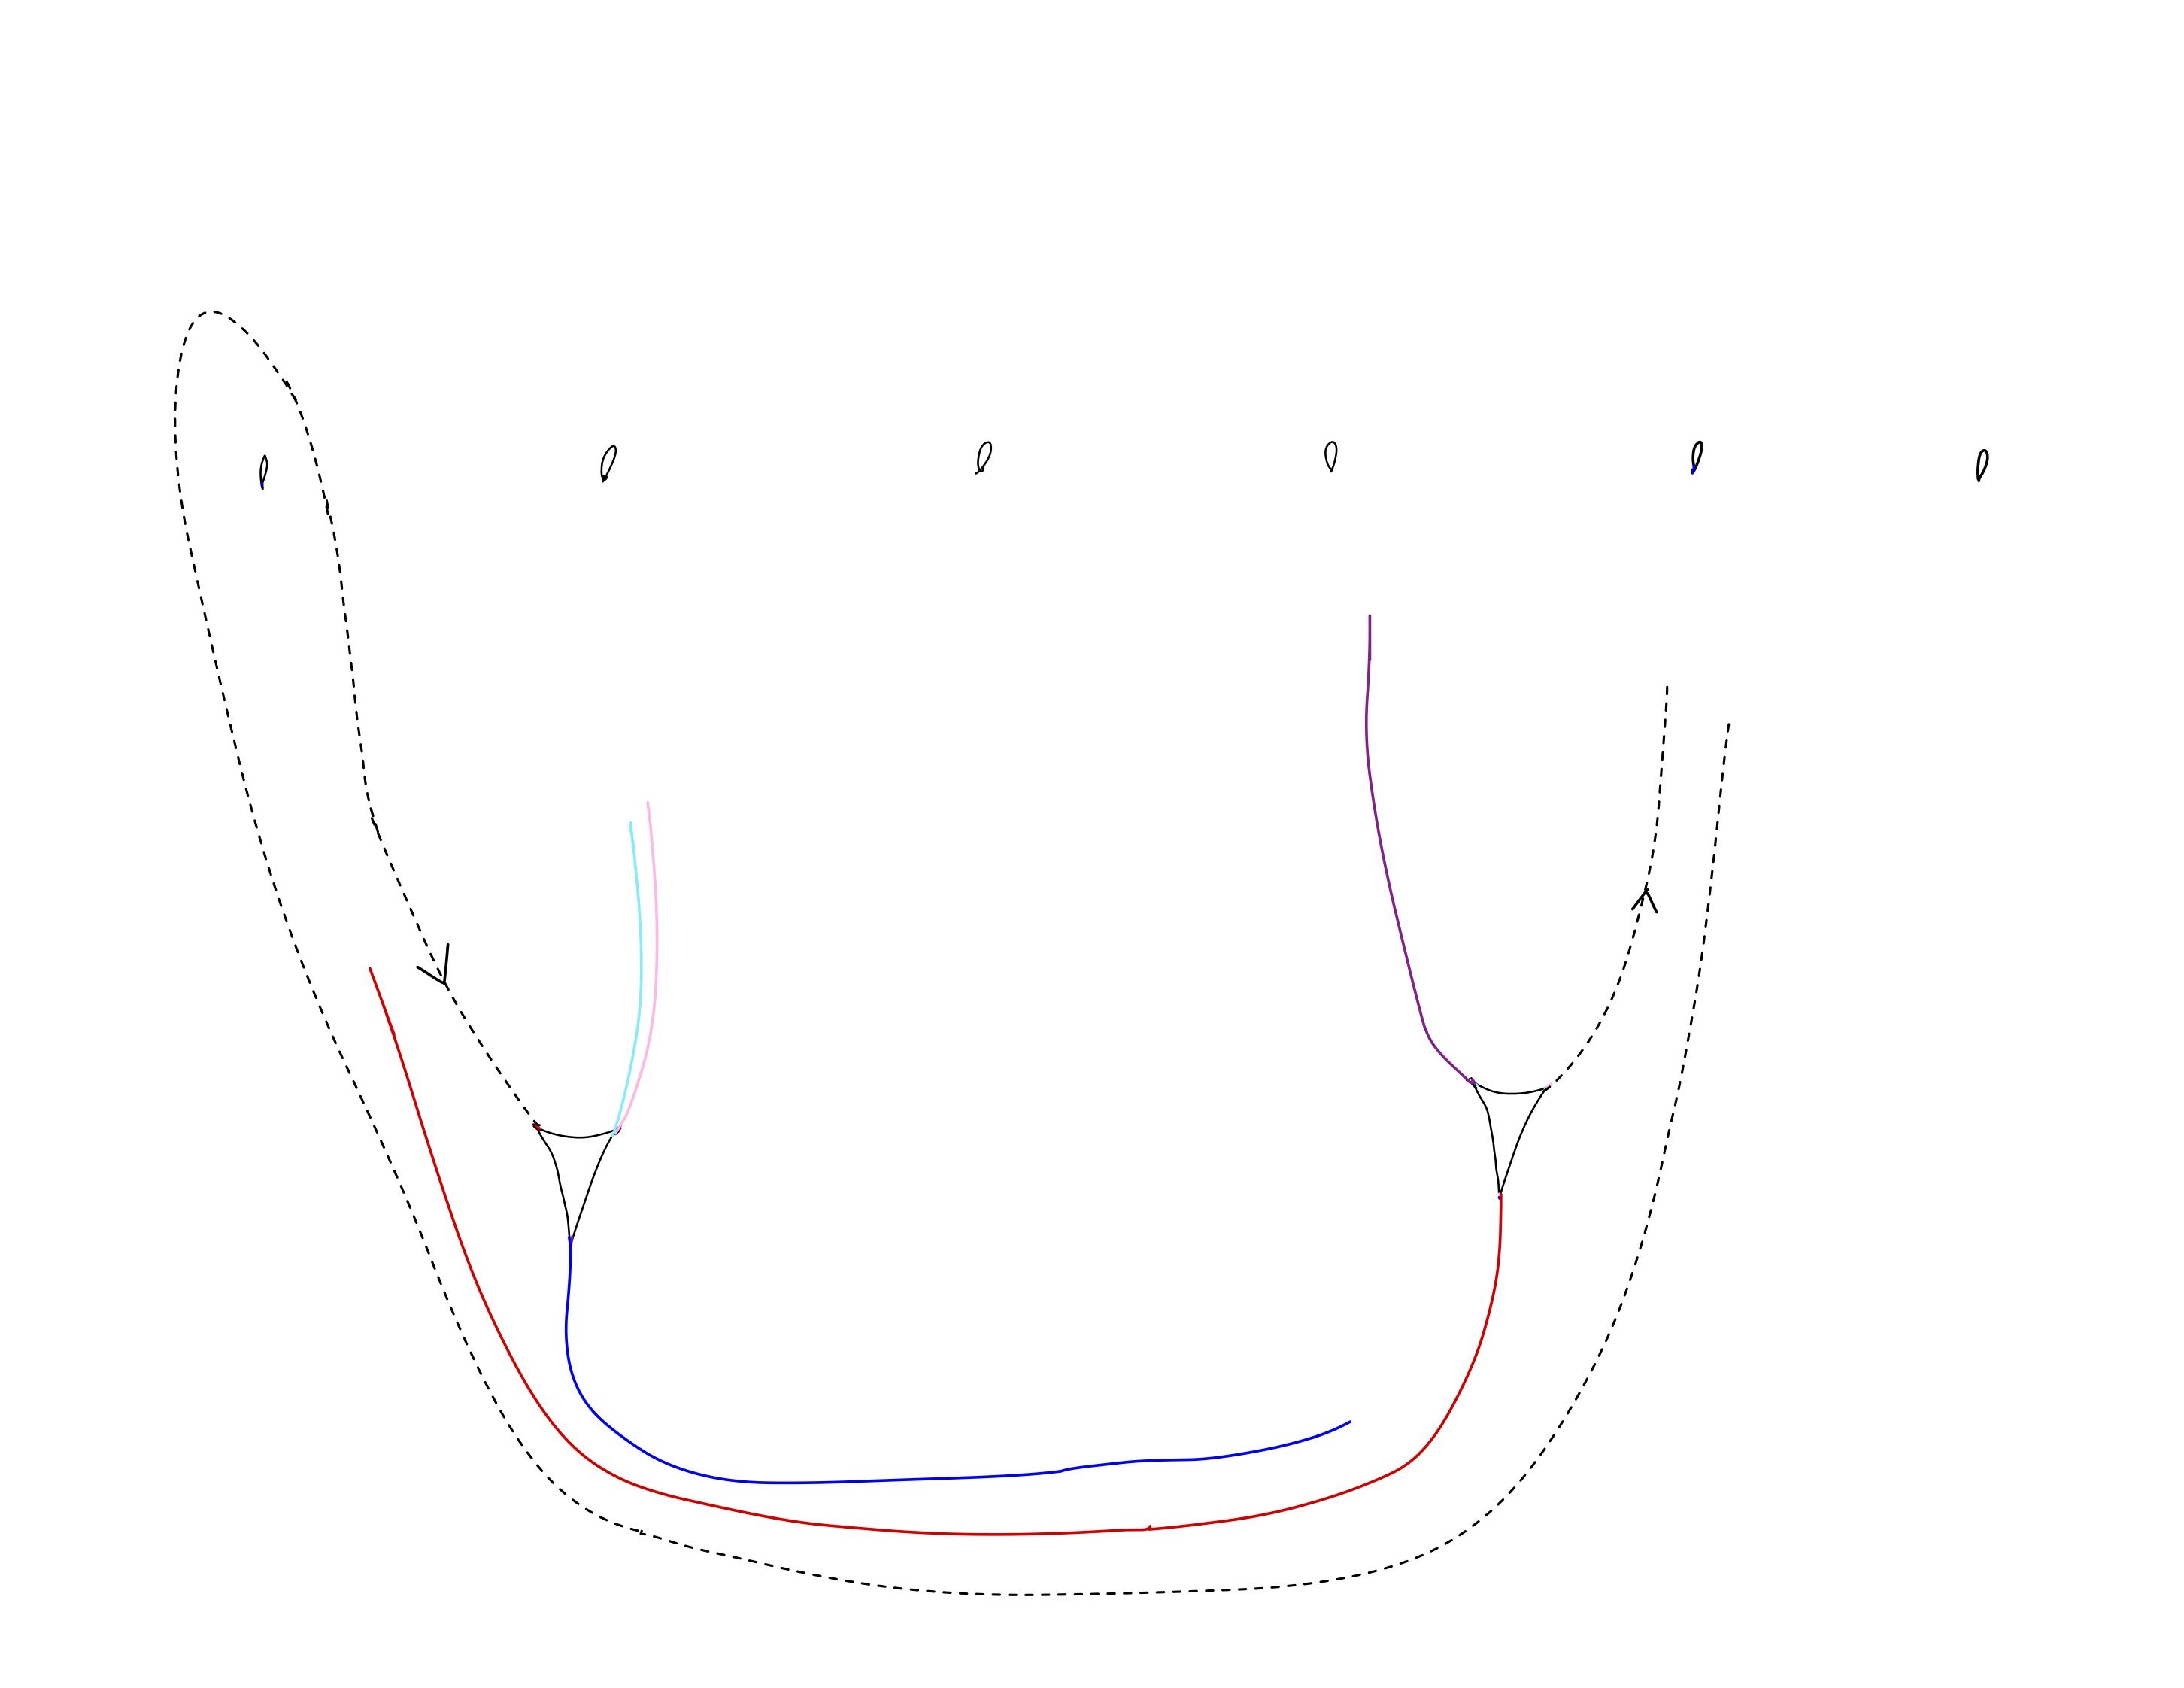
\includegraphics[width=\linewidth]{figures_case_analysis/track17_case_analysis/GBR-12.jpg}
    \caption{GBR12}
    \label{fig:GBR12}
\end{figure}

\begin{figure}[ht]
    \centering
    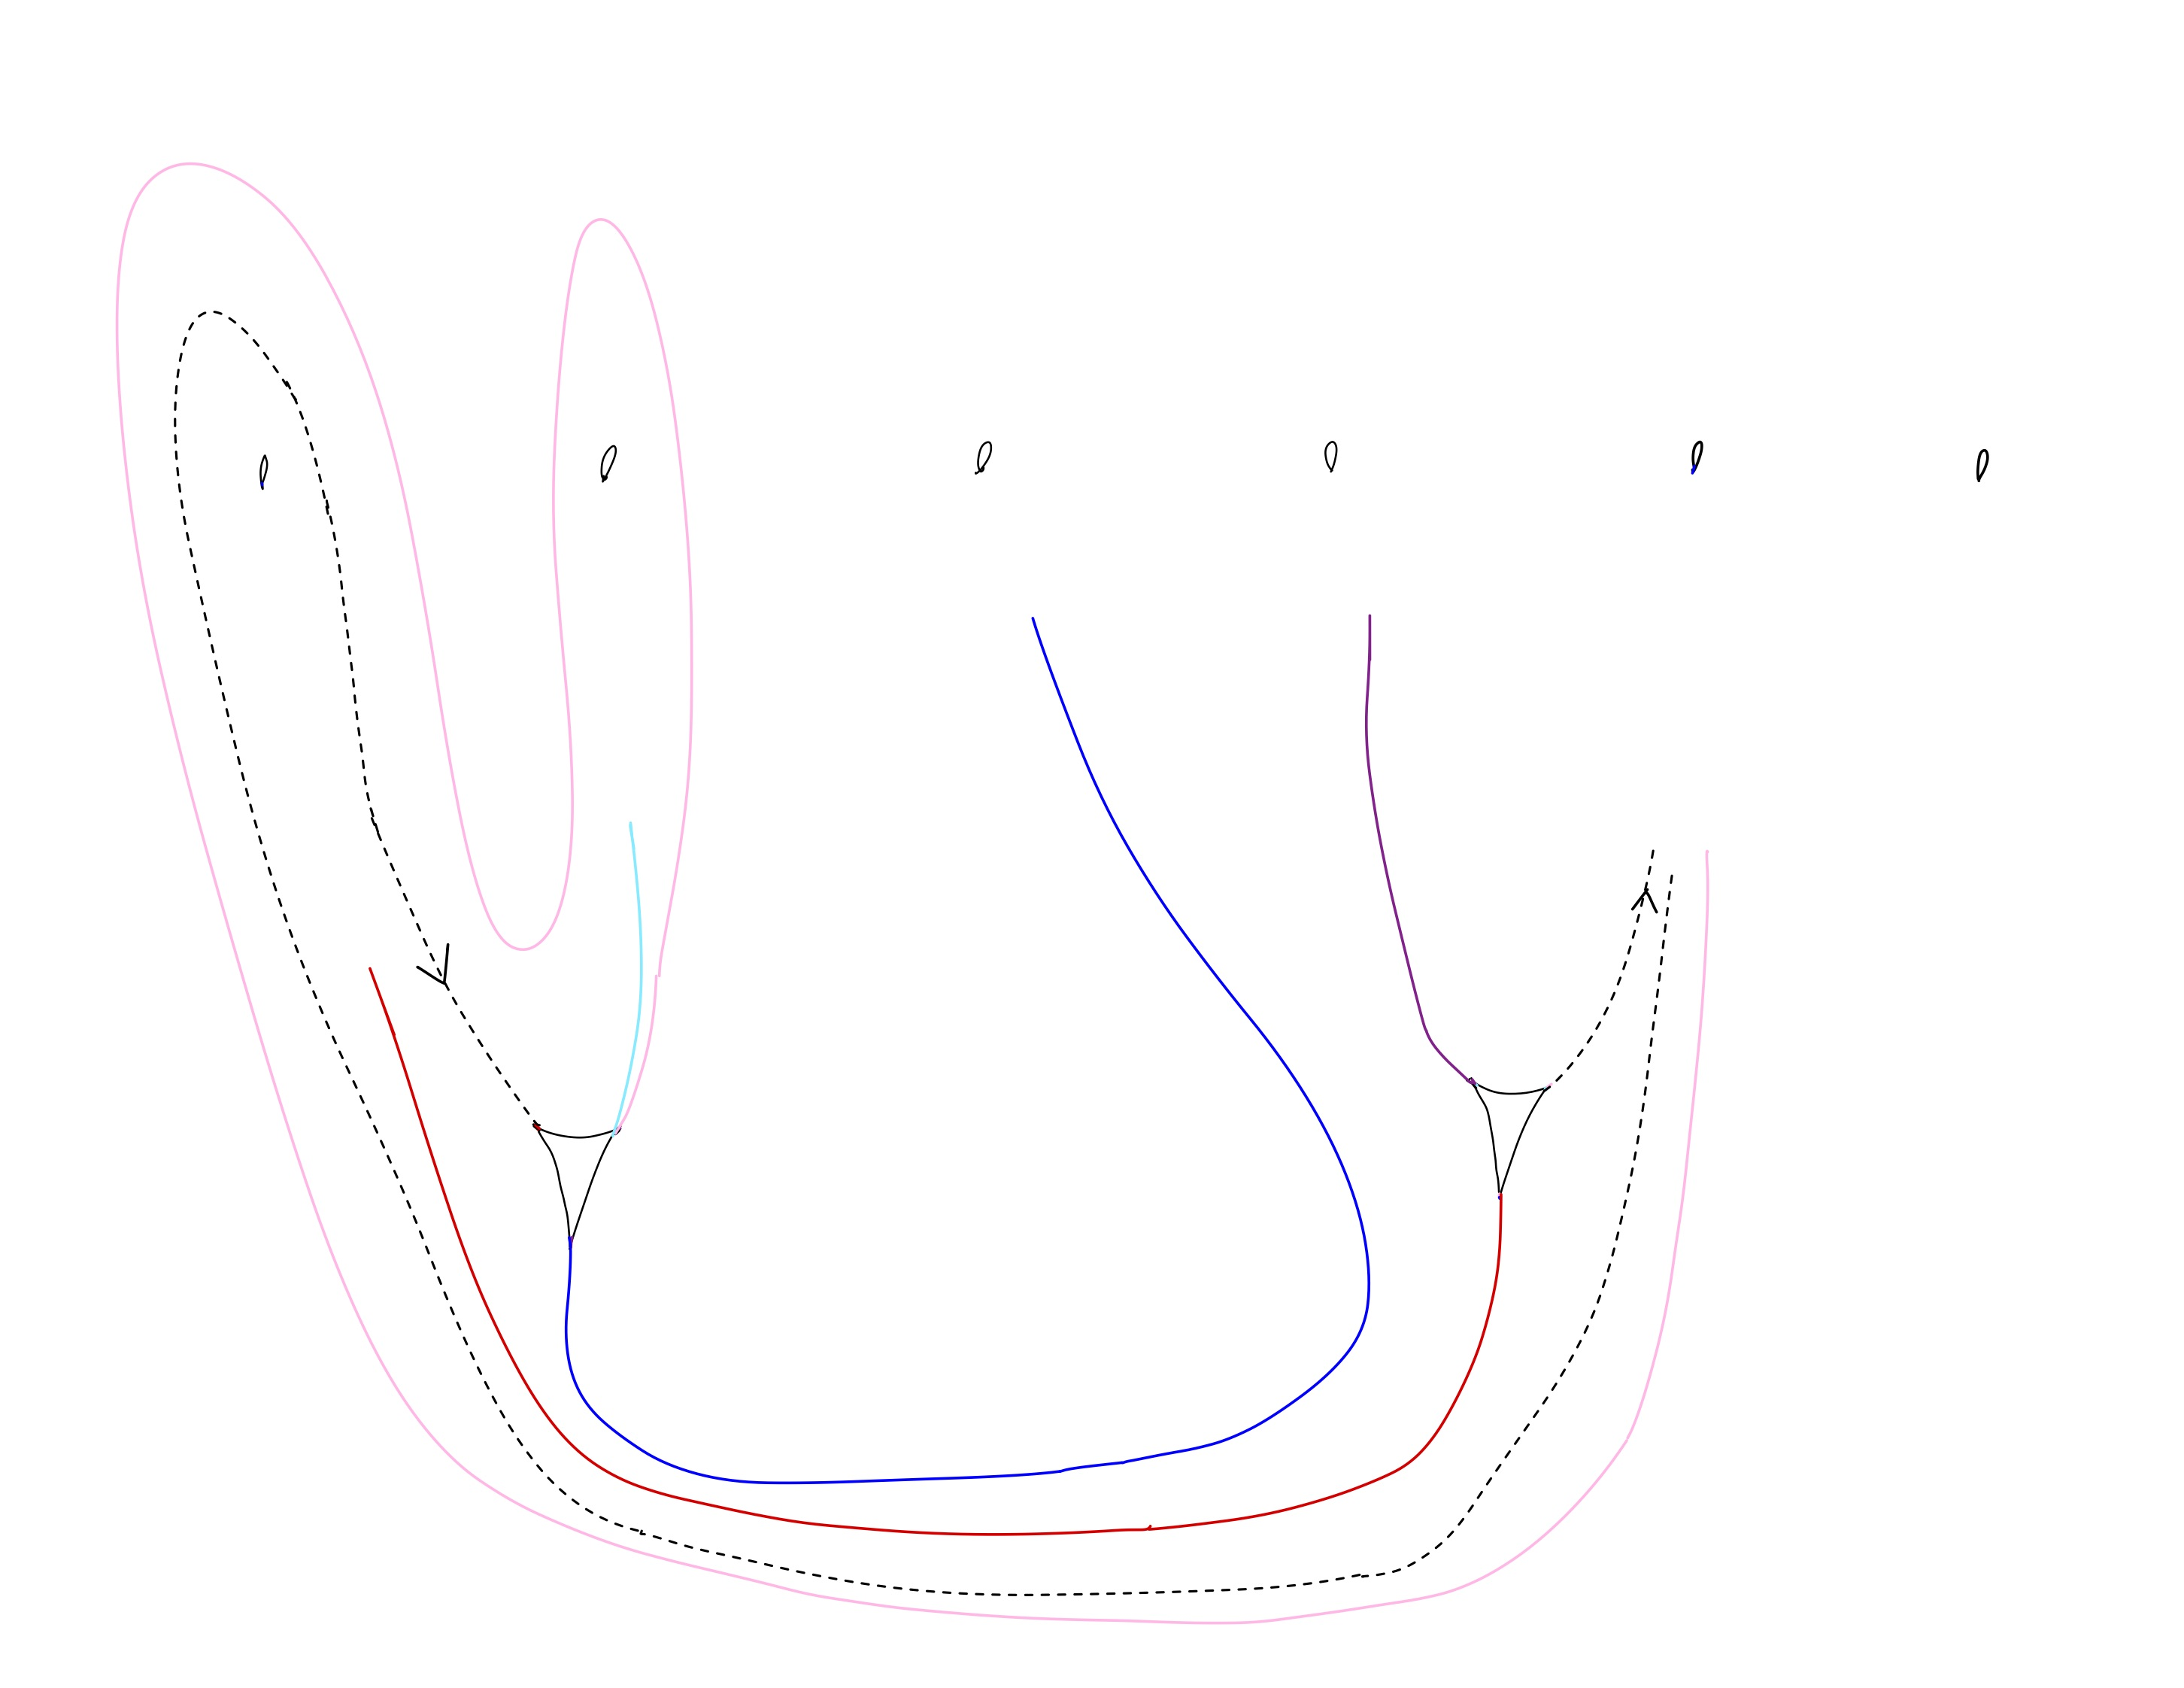
\includegraphics[width=\linewidth]{figures_case_analysis/track17_case_analysis/GBR-13.jpg}
    \caption{GBR13}
    \label{fig:GBR13}
\end{figure}

\begin{figure}[ht]
    \centering
    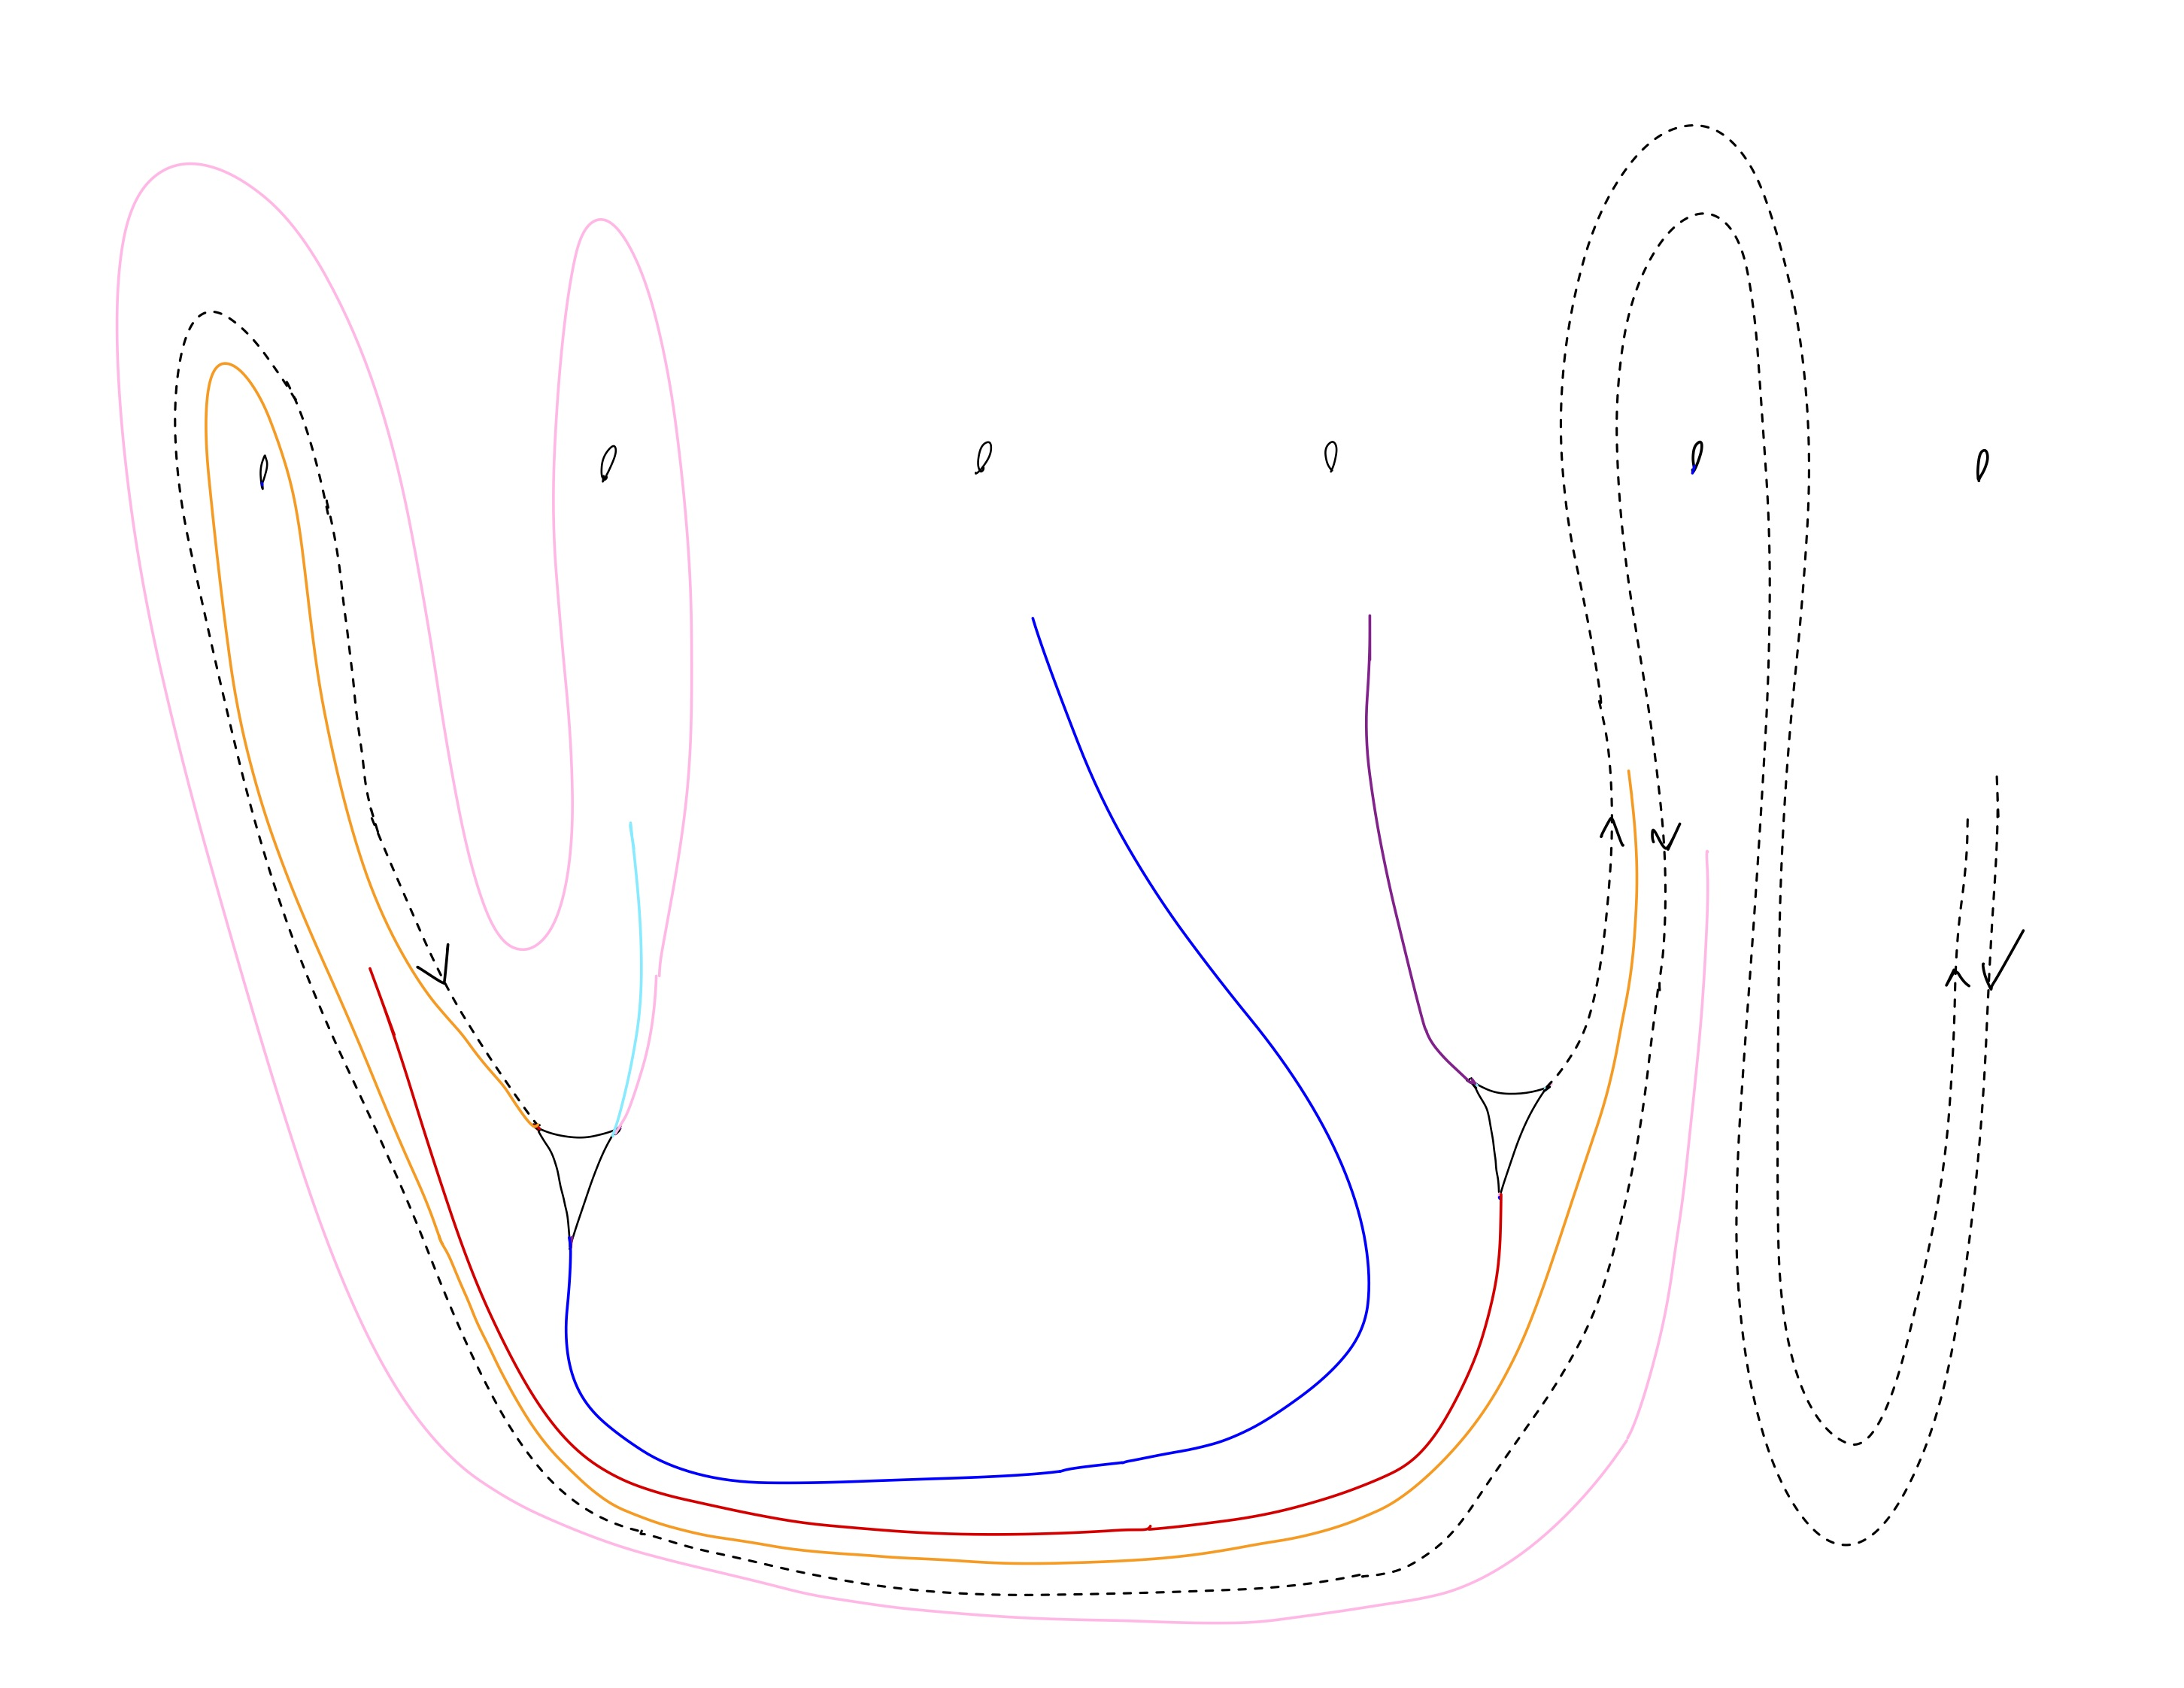
\includegraphics[width=\linewidth]{figures_case_analysis/track17_case_analysis/GBR-14.jpg}
    \caption{GBR14}
    \label{fig:GBR14}
\end{figure}

\begin{figure}[ht]
    \centering
    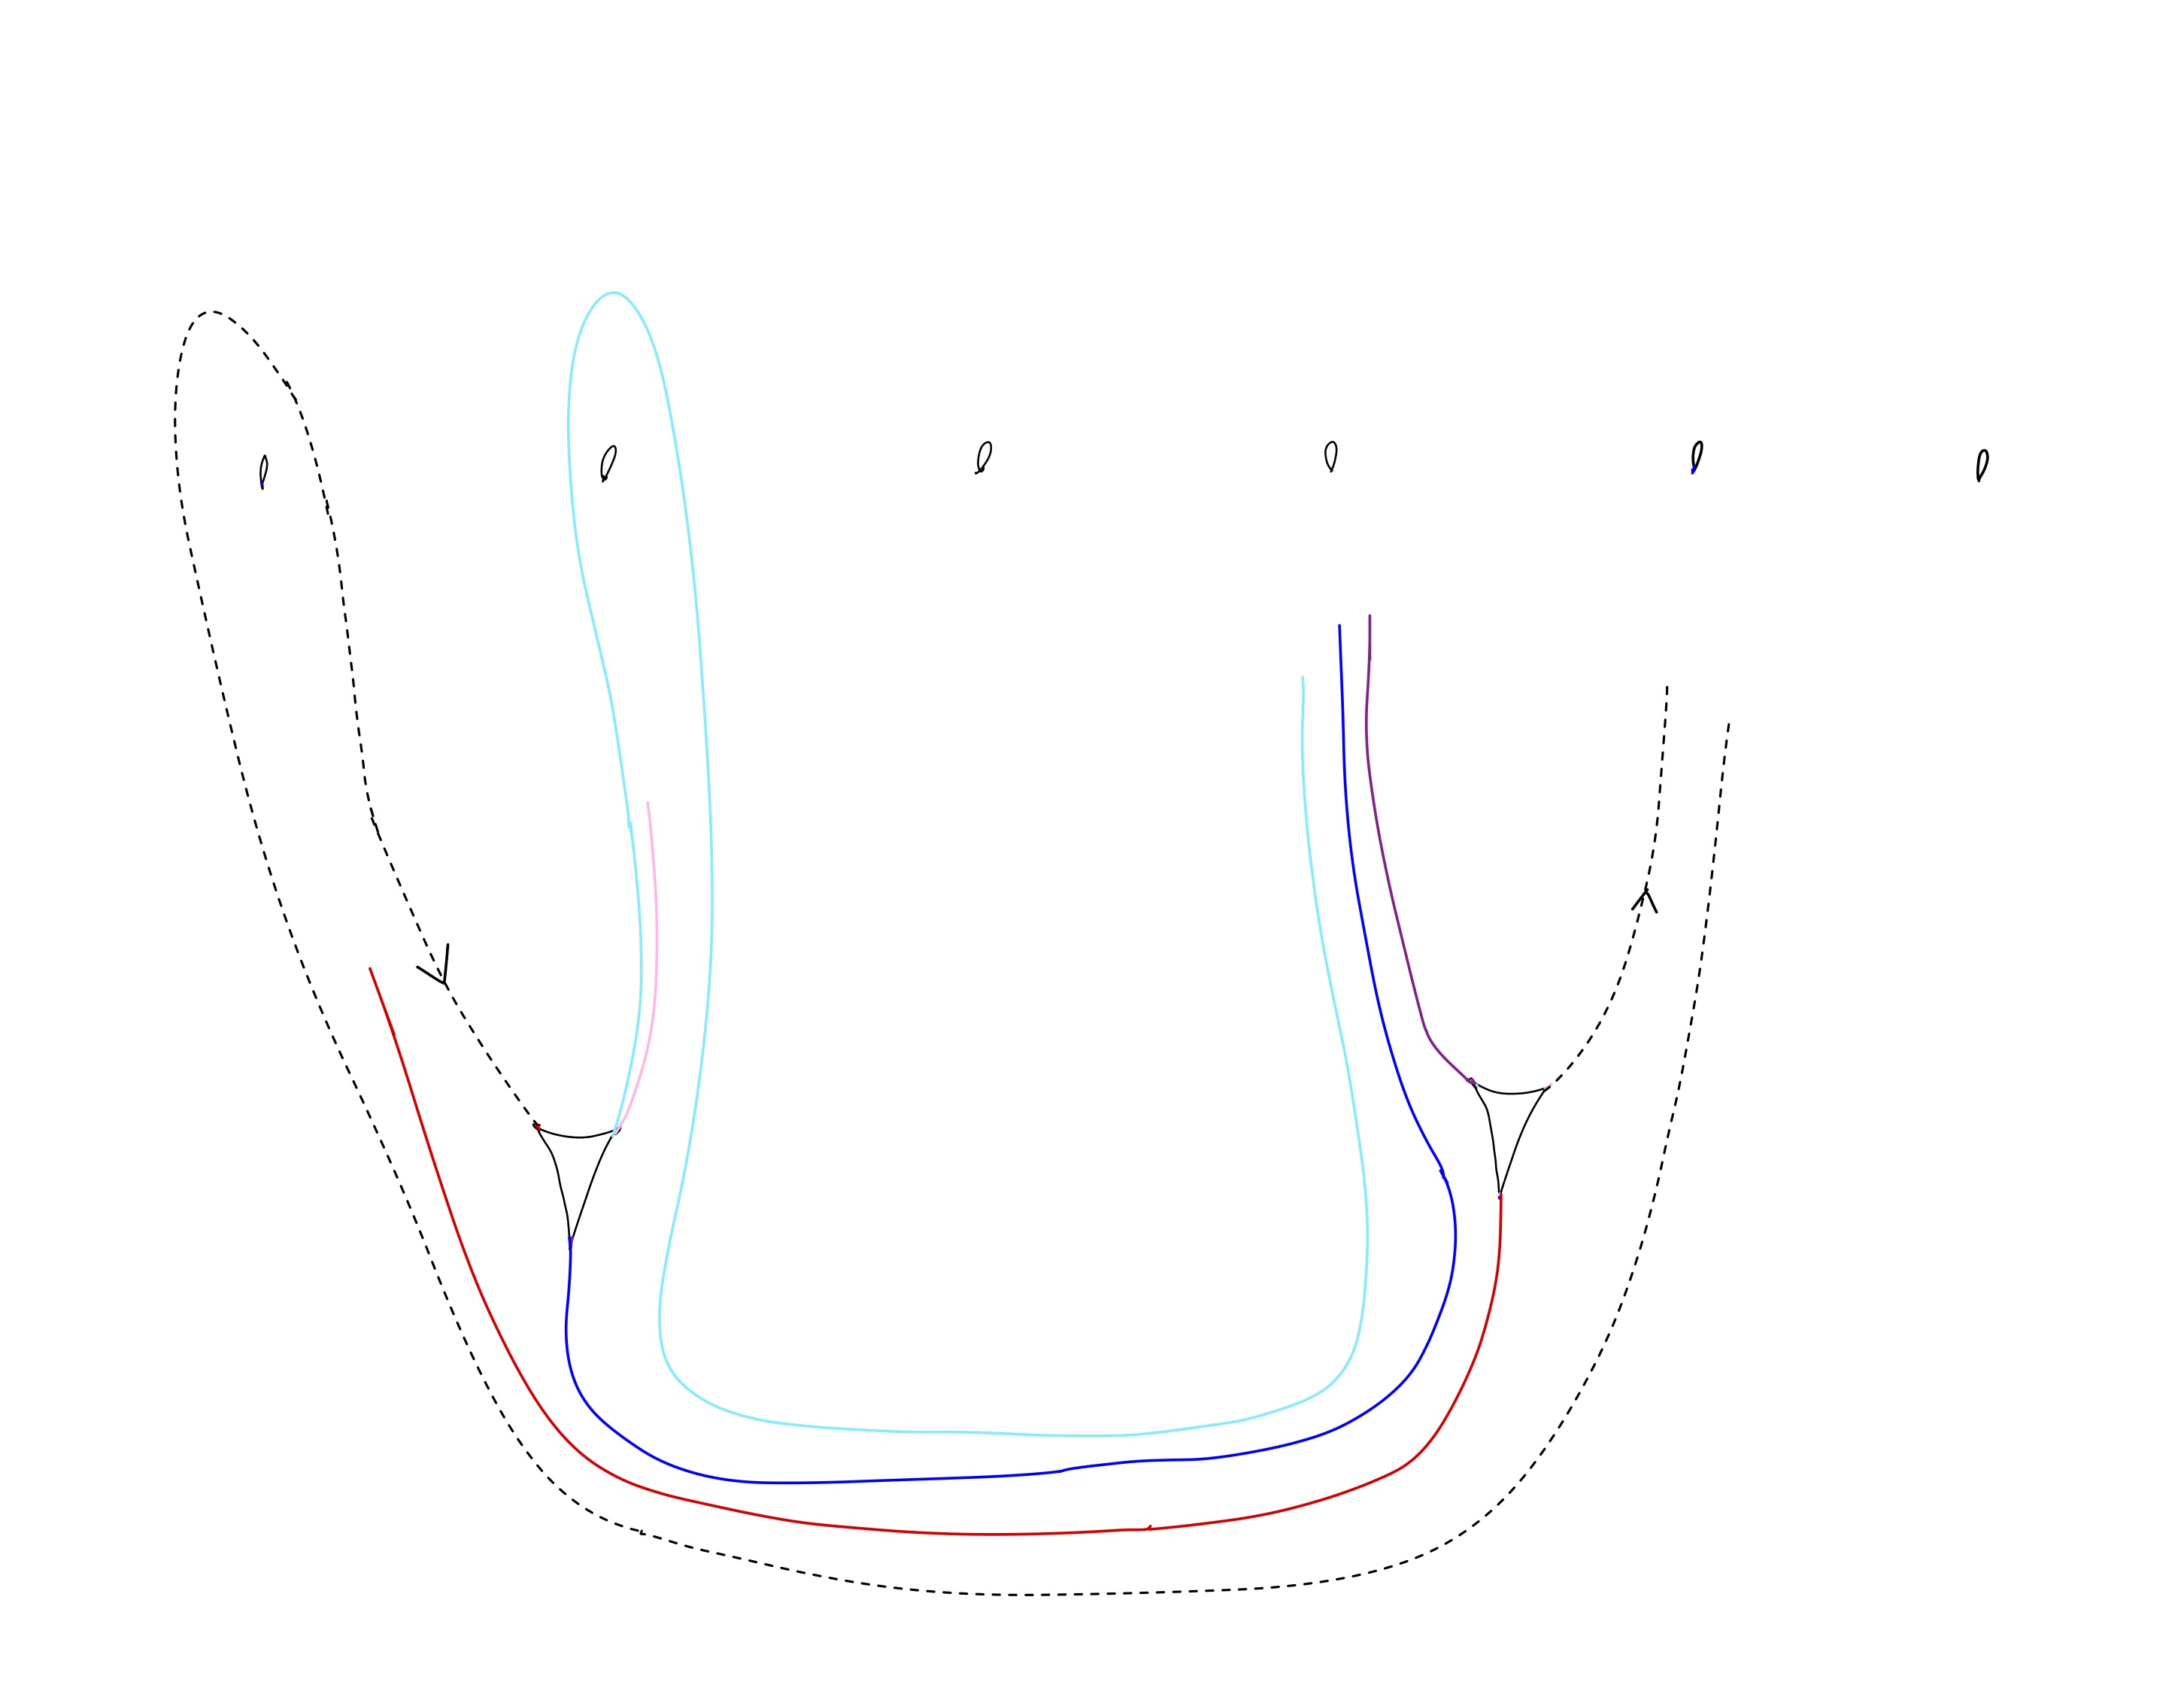
\includegraphics[width=\linewidth]{figures_case_analysis/track17_case_analysis/GBR-15.jpg}
    \caption{GBR15}
    \label{fig:GBR15}
\end{figure}

\begin{figure}[ht]
    \centering
    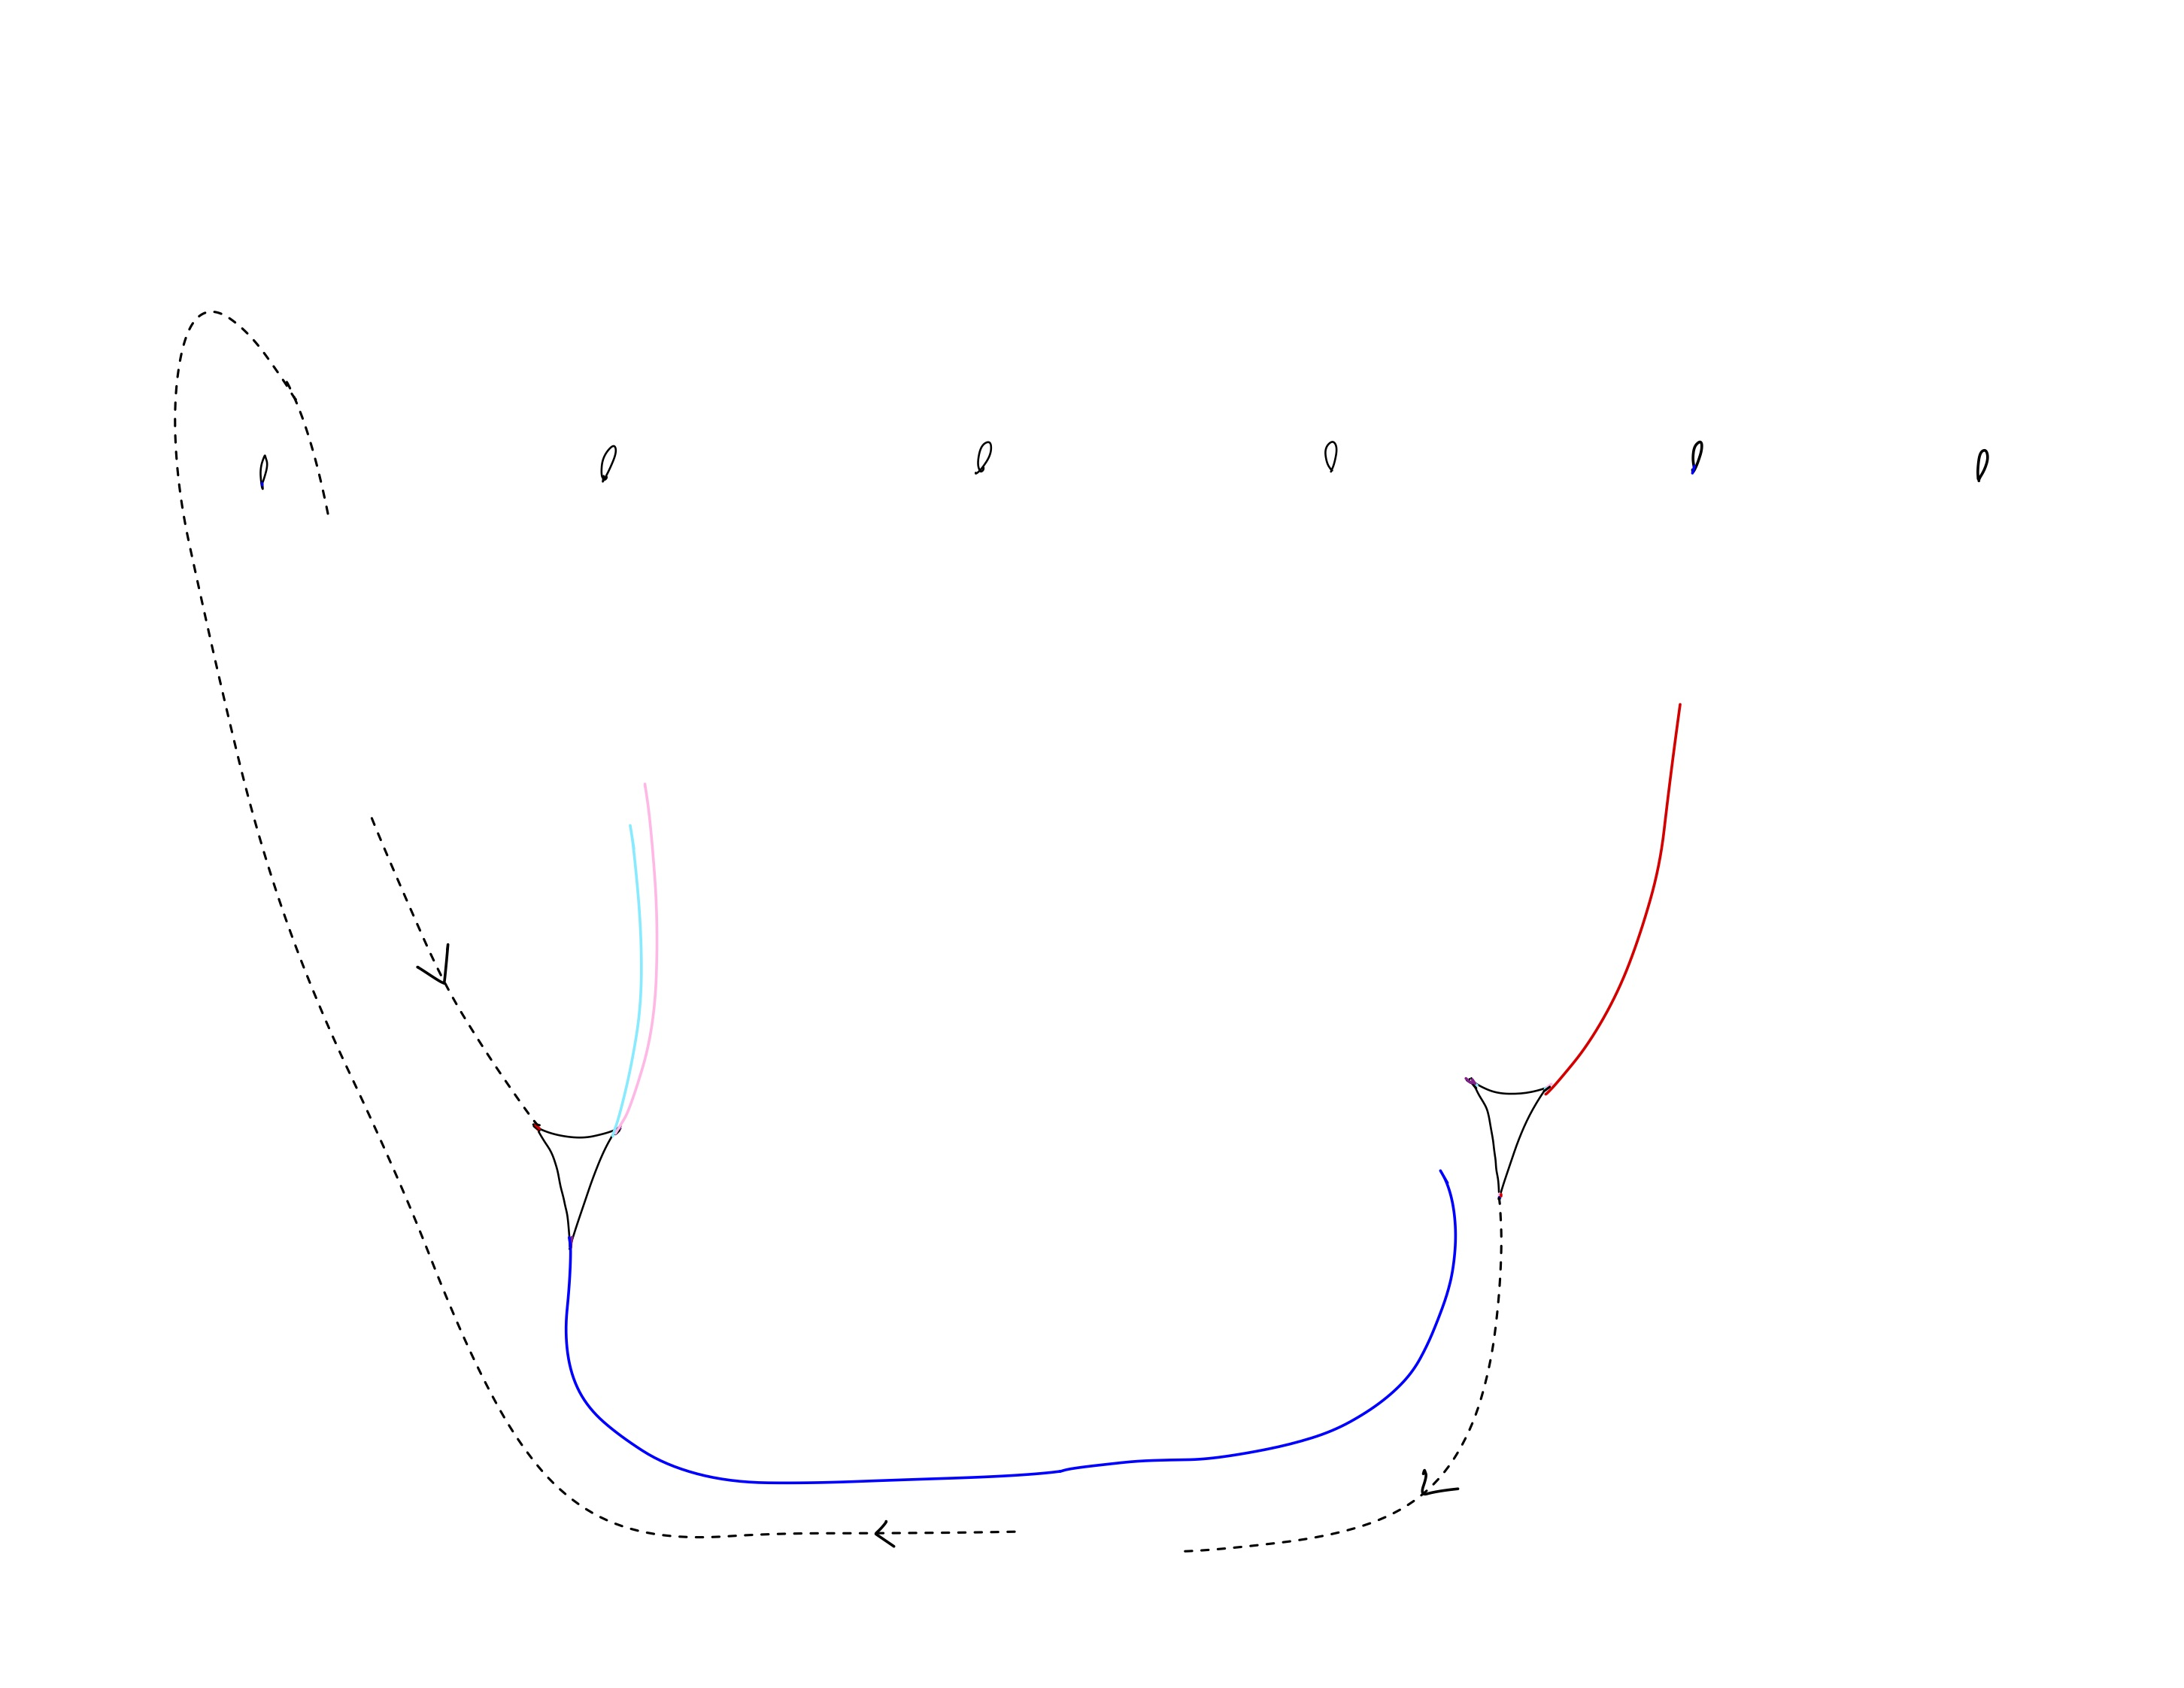
\includegraphics[width=\linewidth]{figures_case_analysis/track17_case_analysis/GBR-16.jpg}
    \caption{GBR16}
    \label{fig:GBR16}
\end{figure}

\begin{figure}[ht]
    \centering
    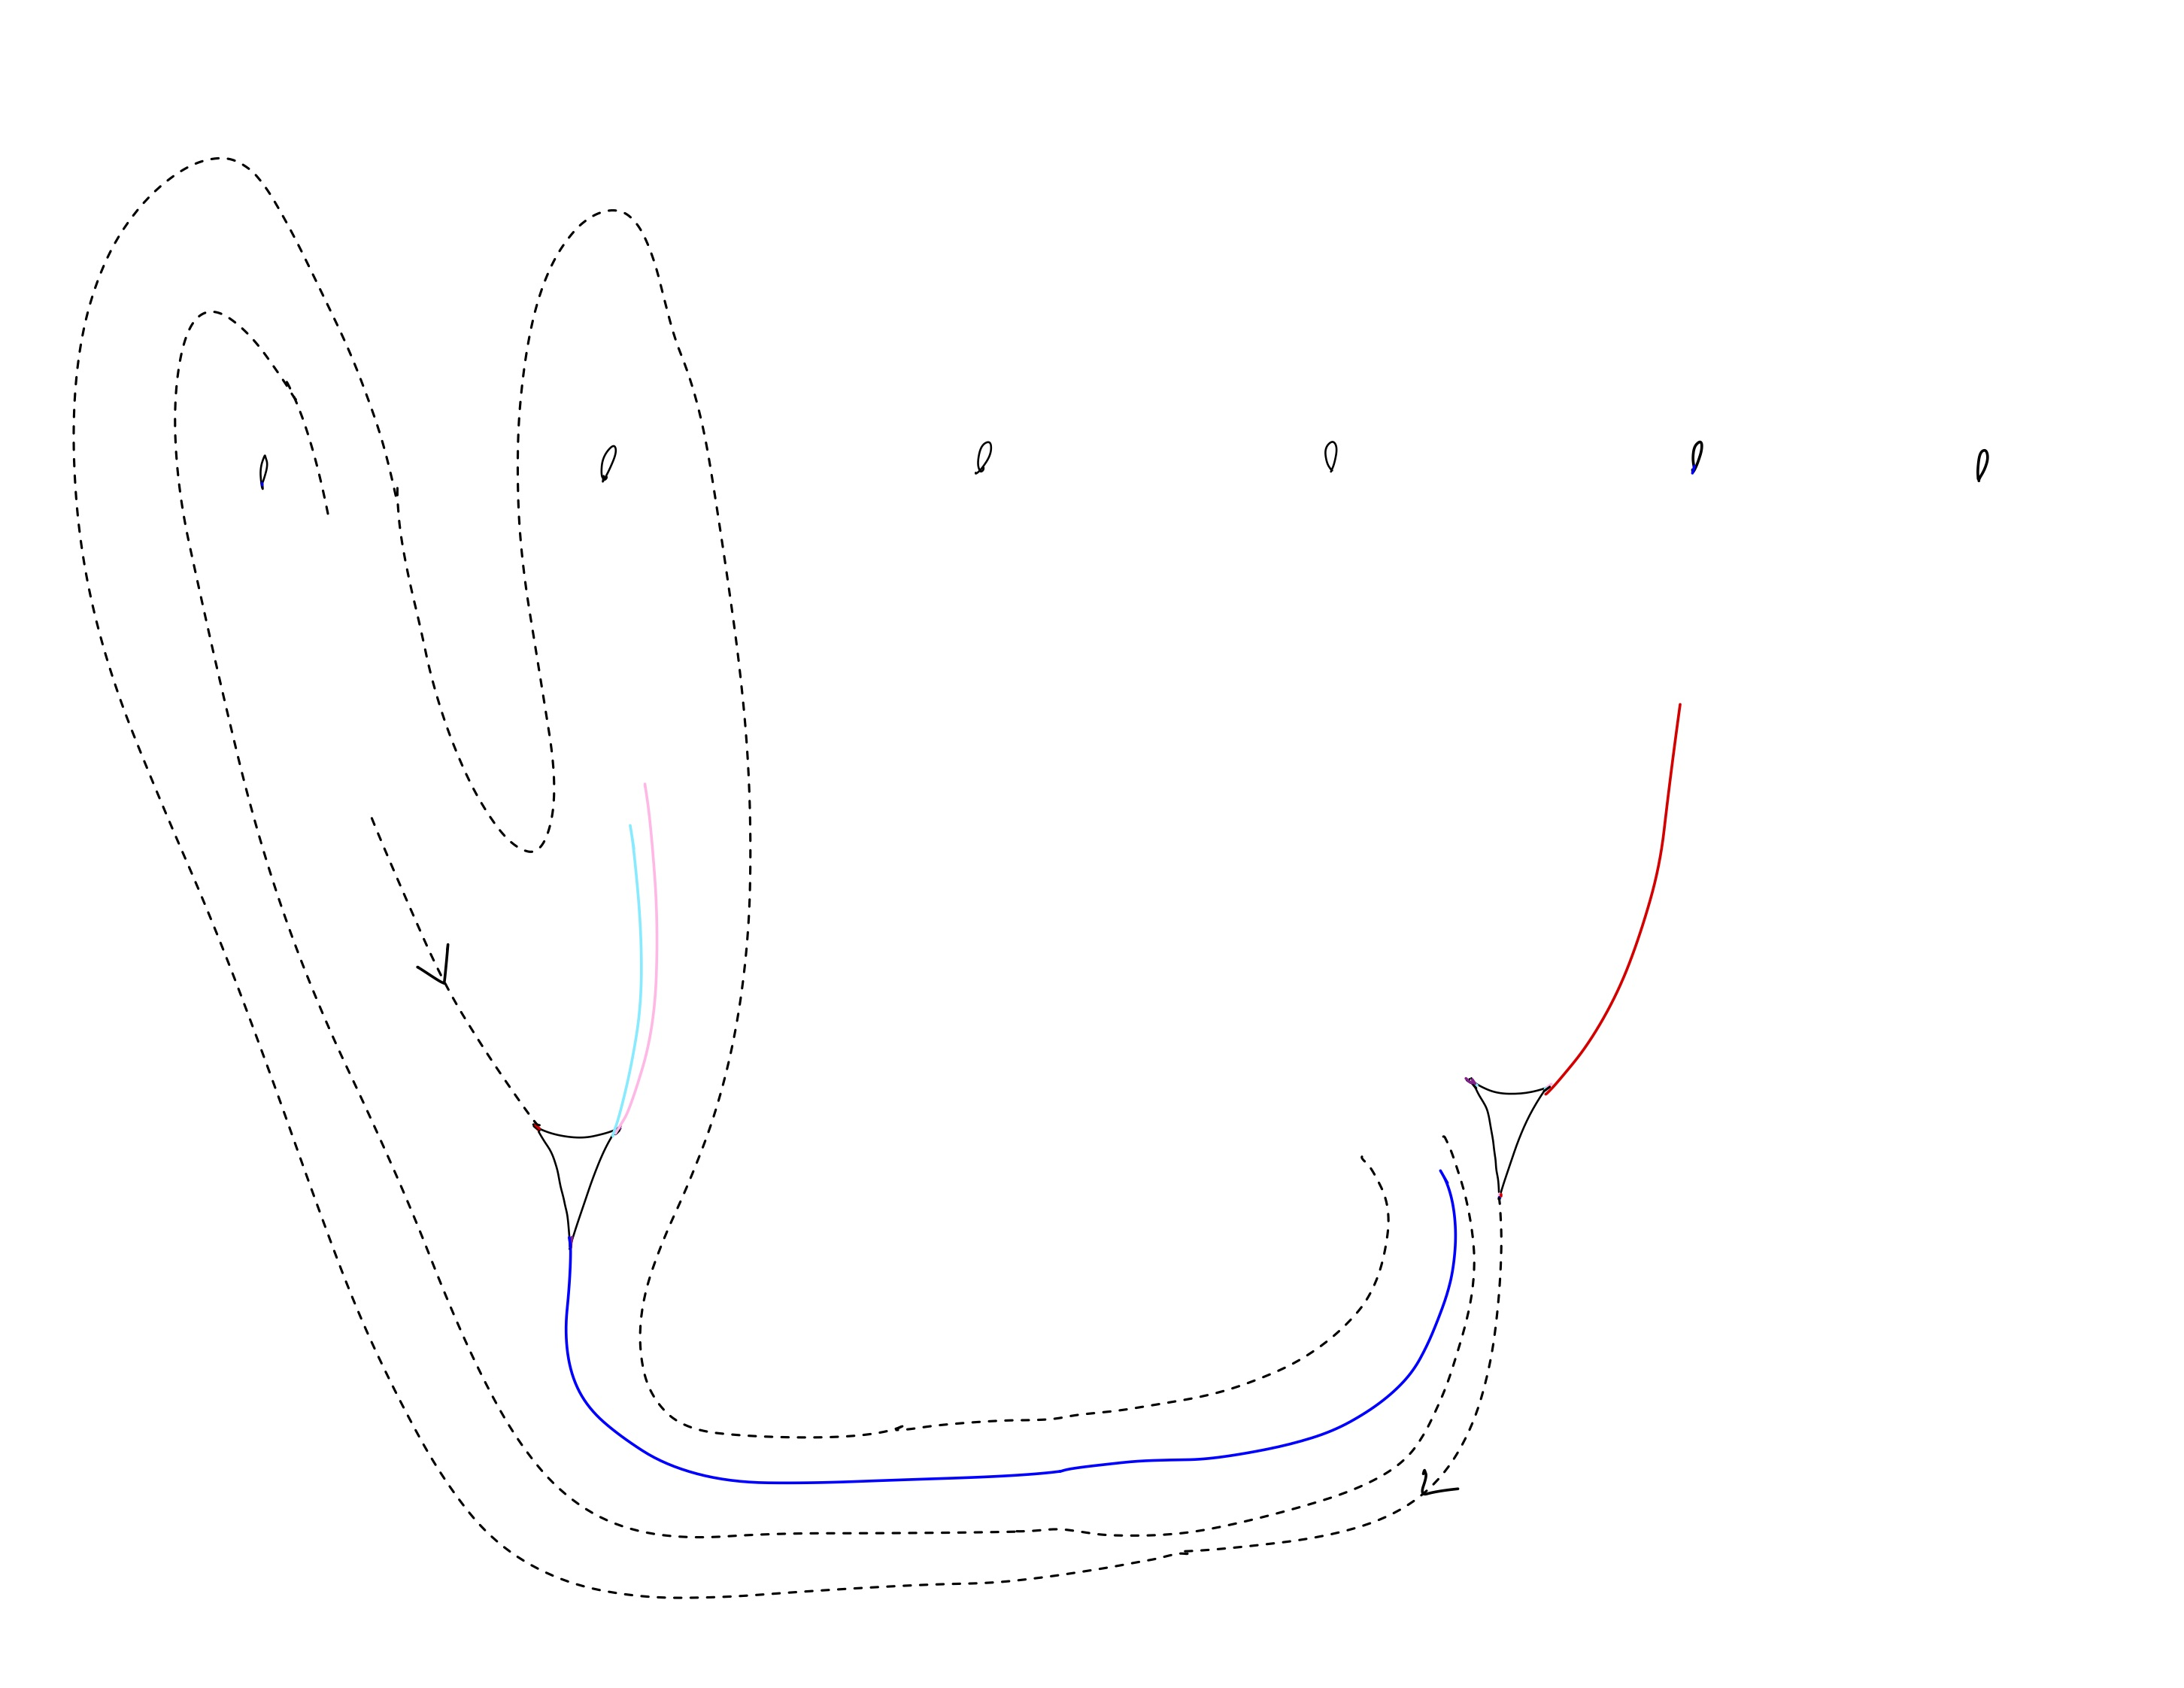
\includegraphics[width=\linewidth]{figures_case_analysis/track17_case_analysis/GBR-17.jpg}
    \caption{GBR17}
    \label{fig:GBR17}
\end{figure}

\begin{figure}[ht]
    \centering
    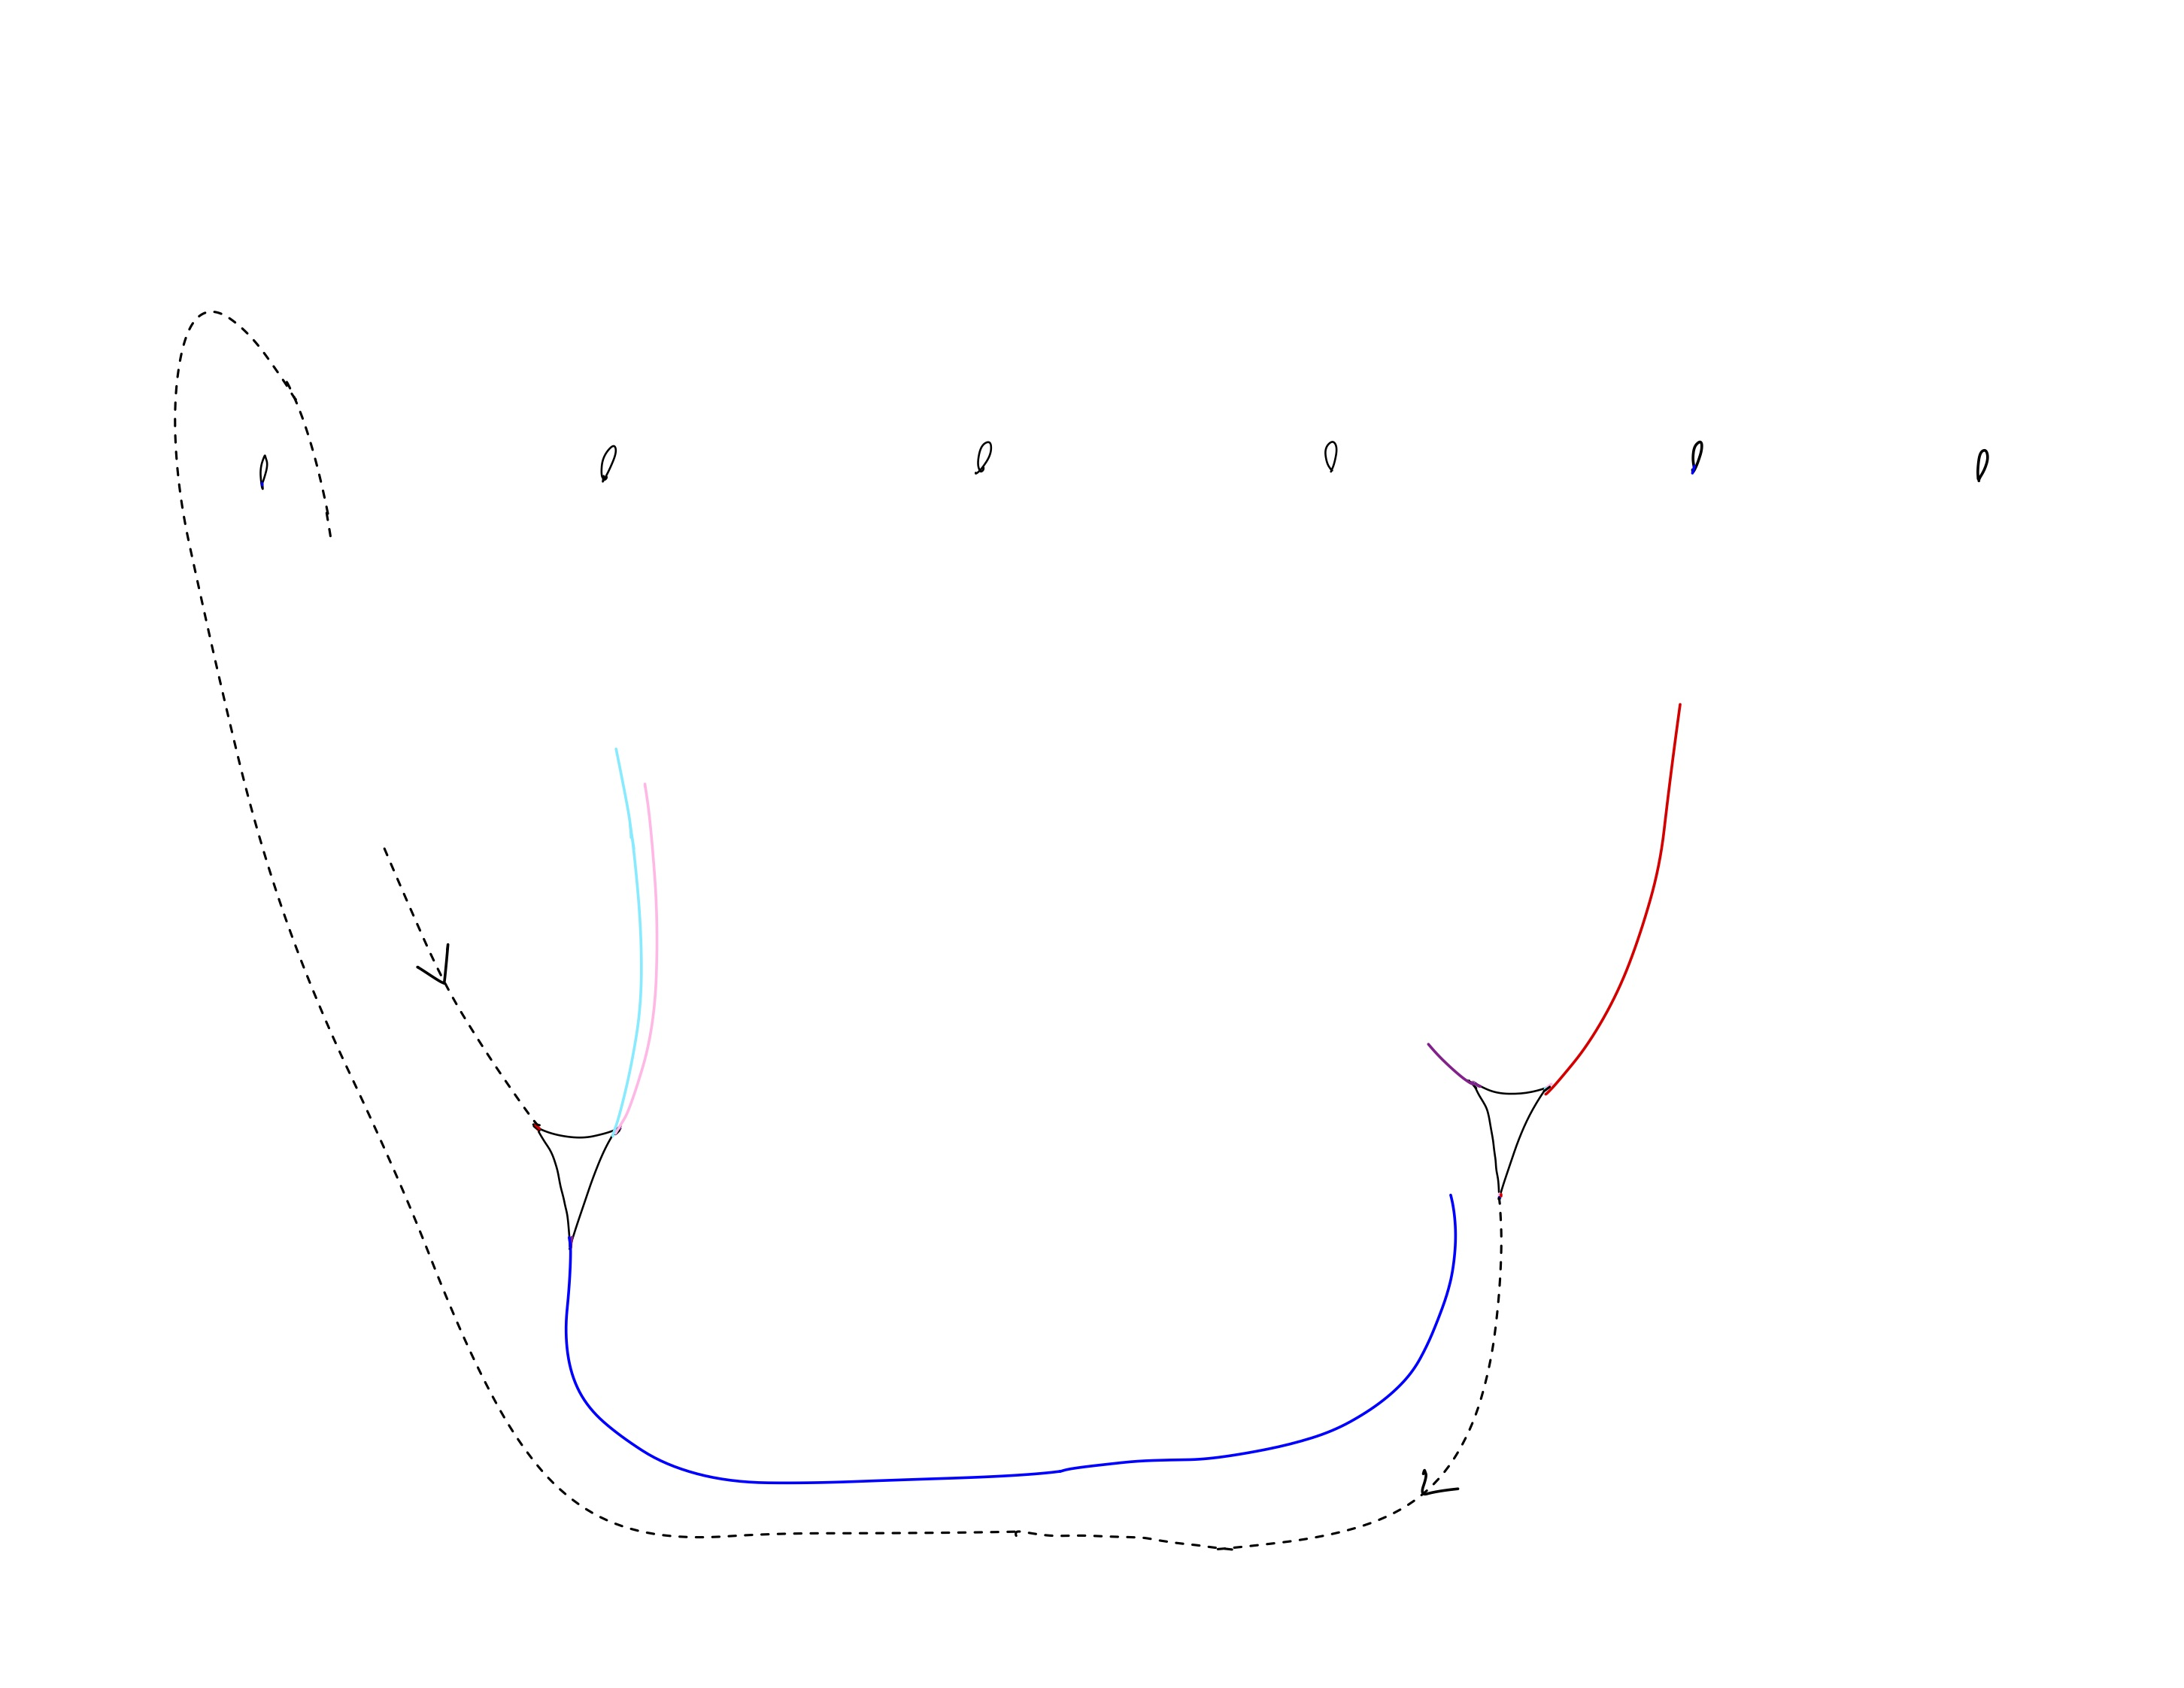
\includegraphics[width=\linewidth]{figures_case_analysis/track17_case_analysis/GBR-18.jpg}
    \caption{GBR18}
    \label{fig:GBR18}
\end{figure}
\clearpage

\begin{figure}[ht]
    \centering
    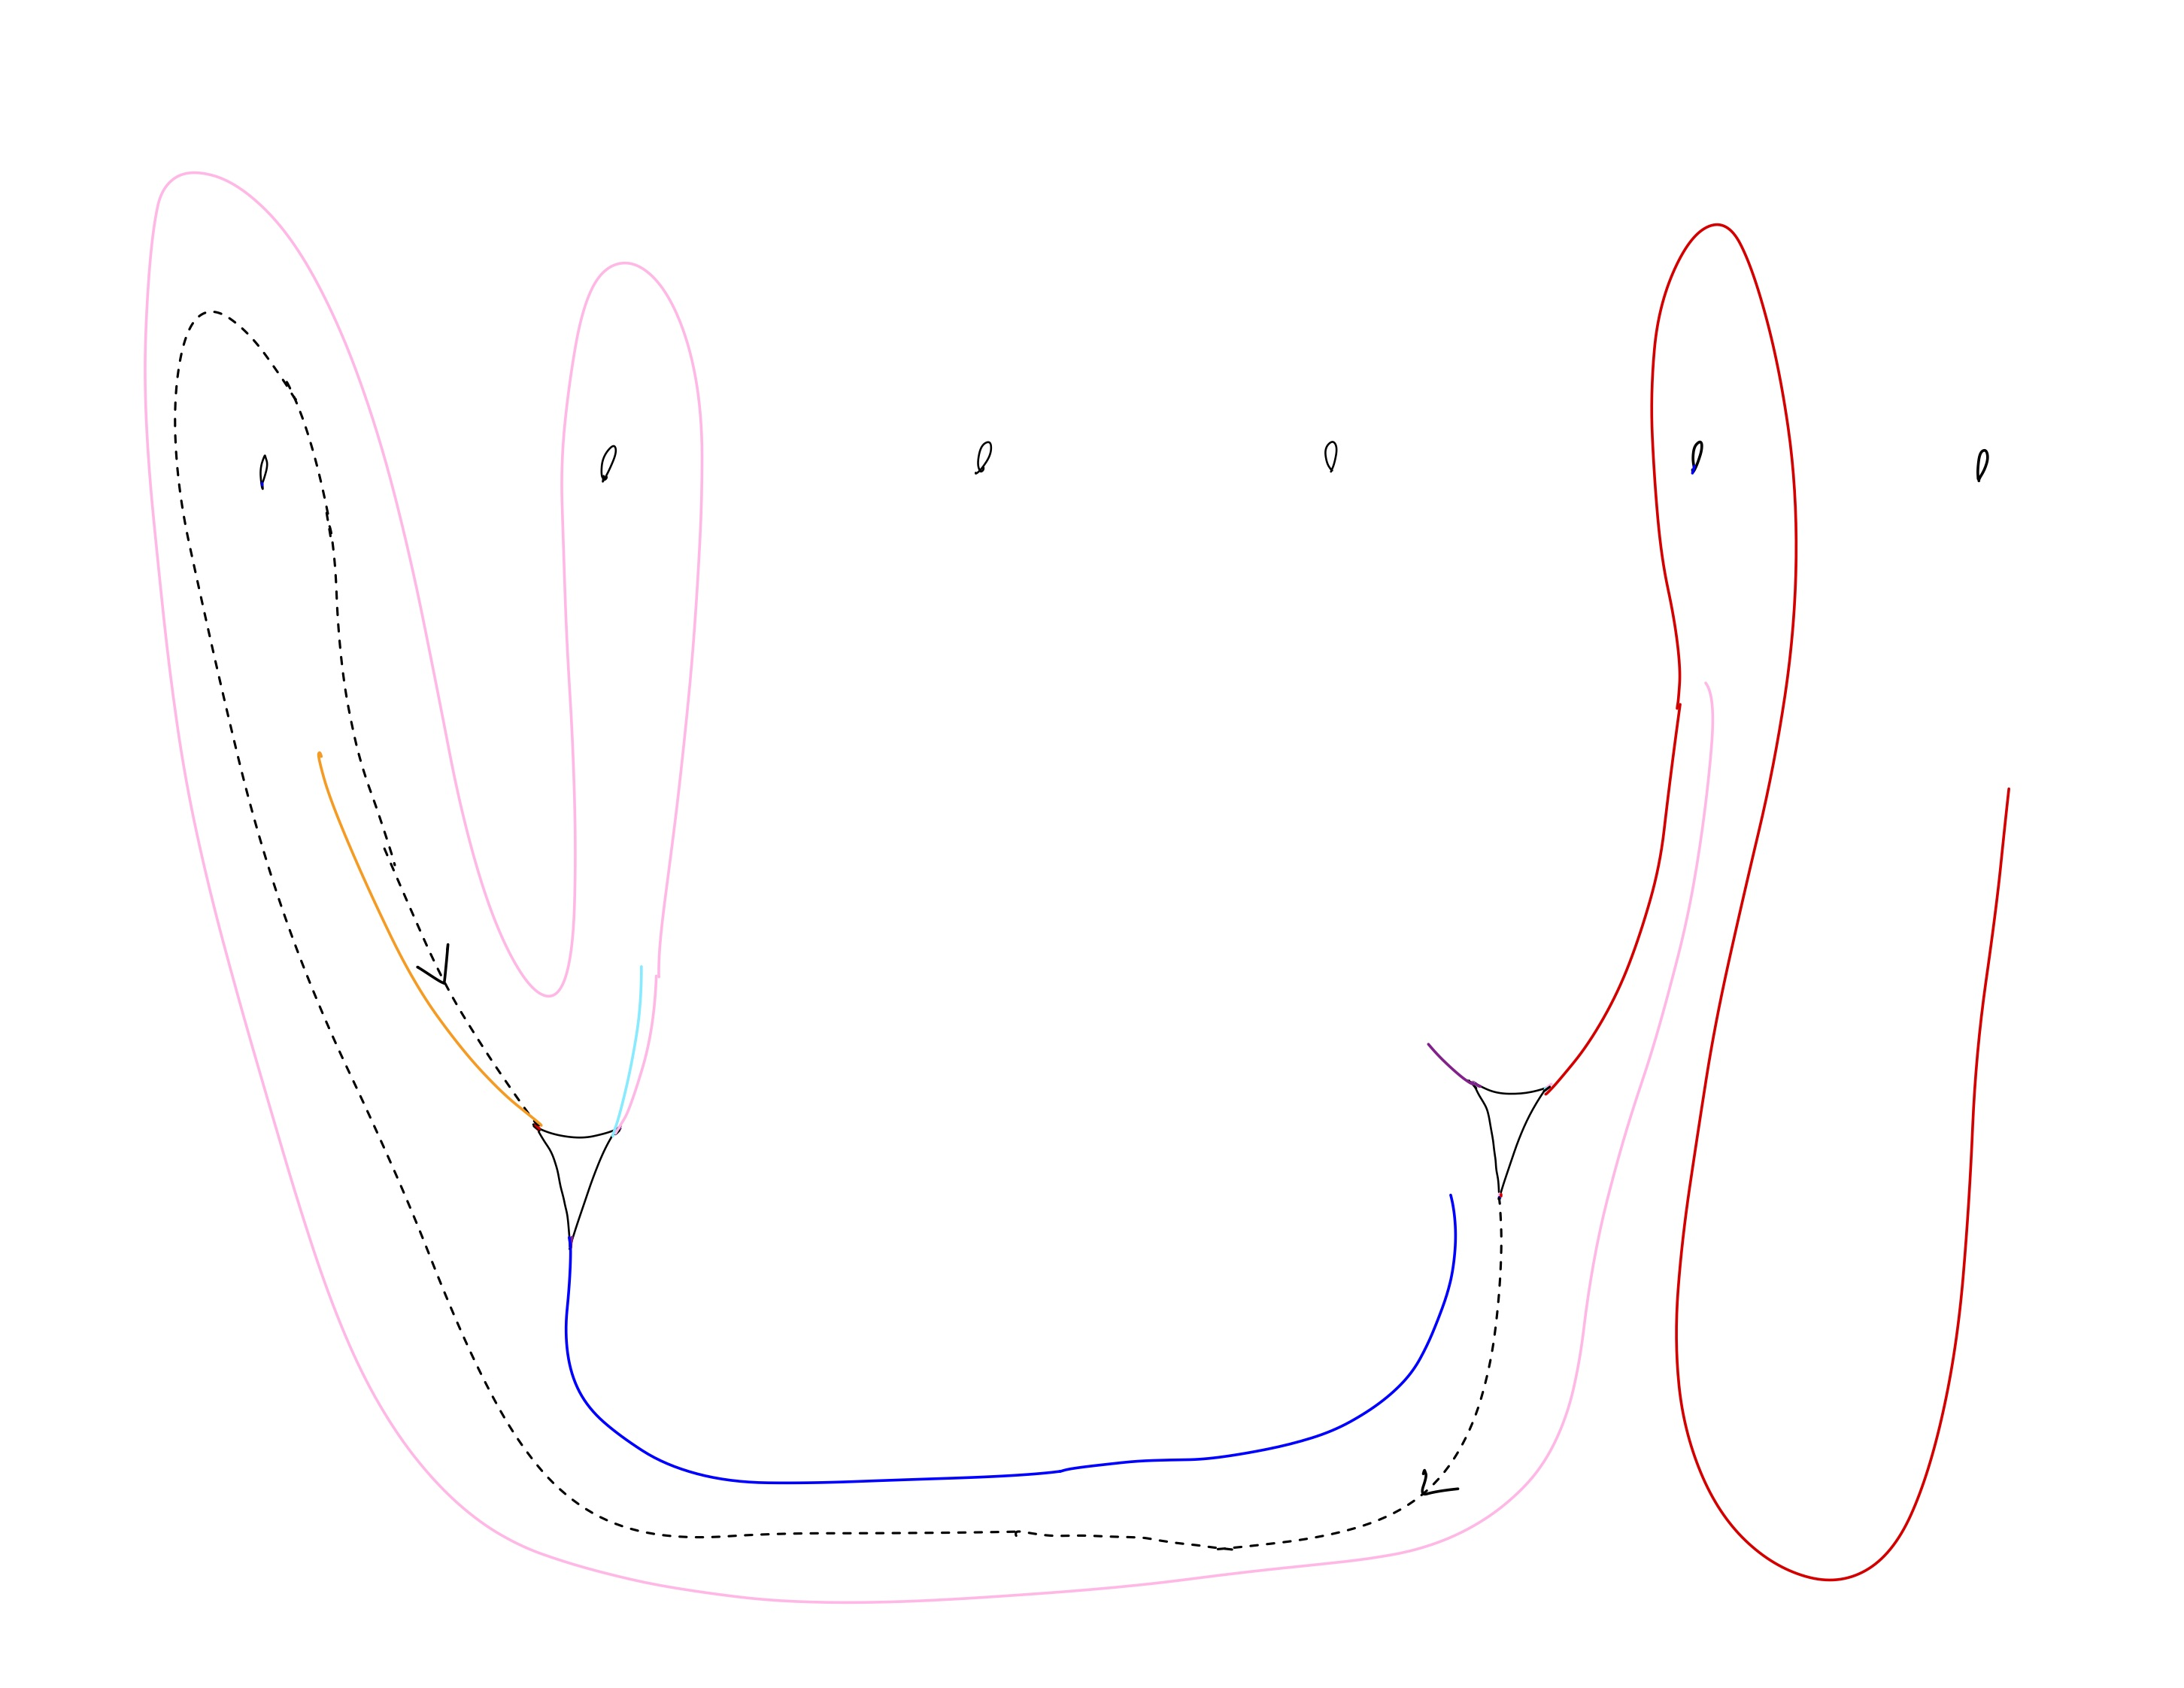
\includegraphics[width=\linewidth]{figures_case_analysis/track17_case_analysis/Boke-01.jpg}
    \caption{Boke1}
    \label{fig:Boke1}
\end{figure}

\begin{figure}[ht]
    \centering
    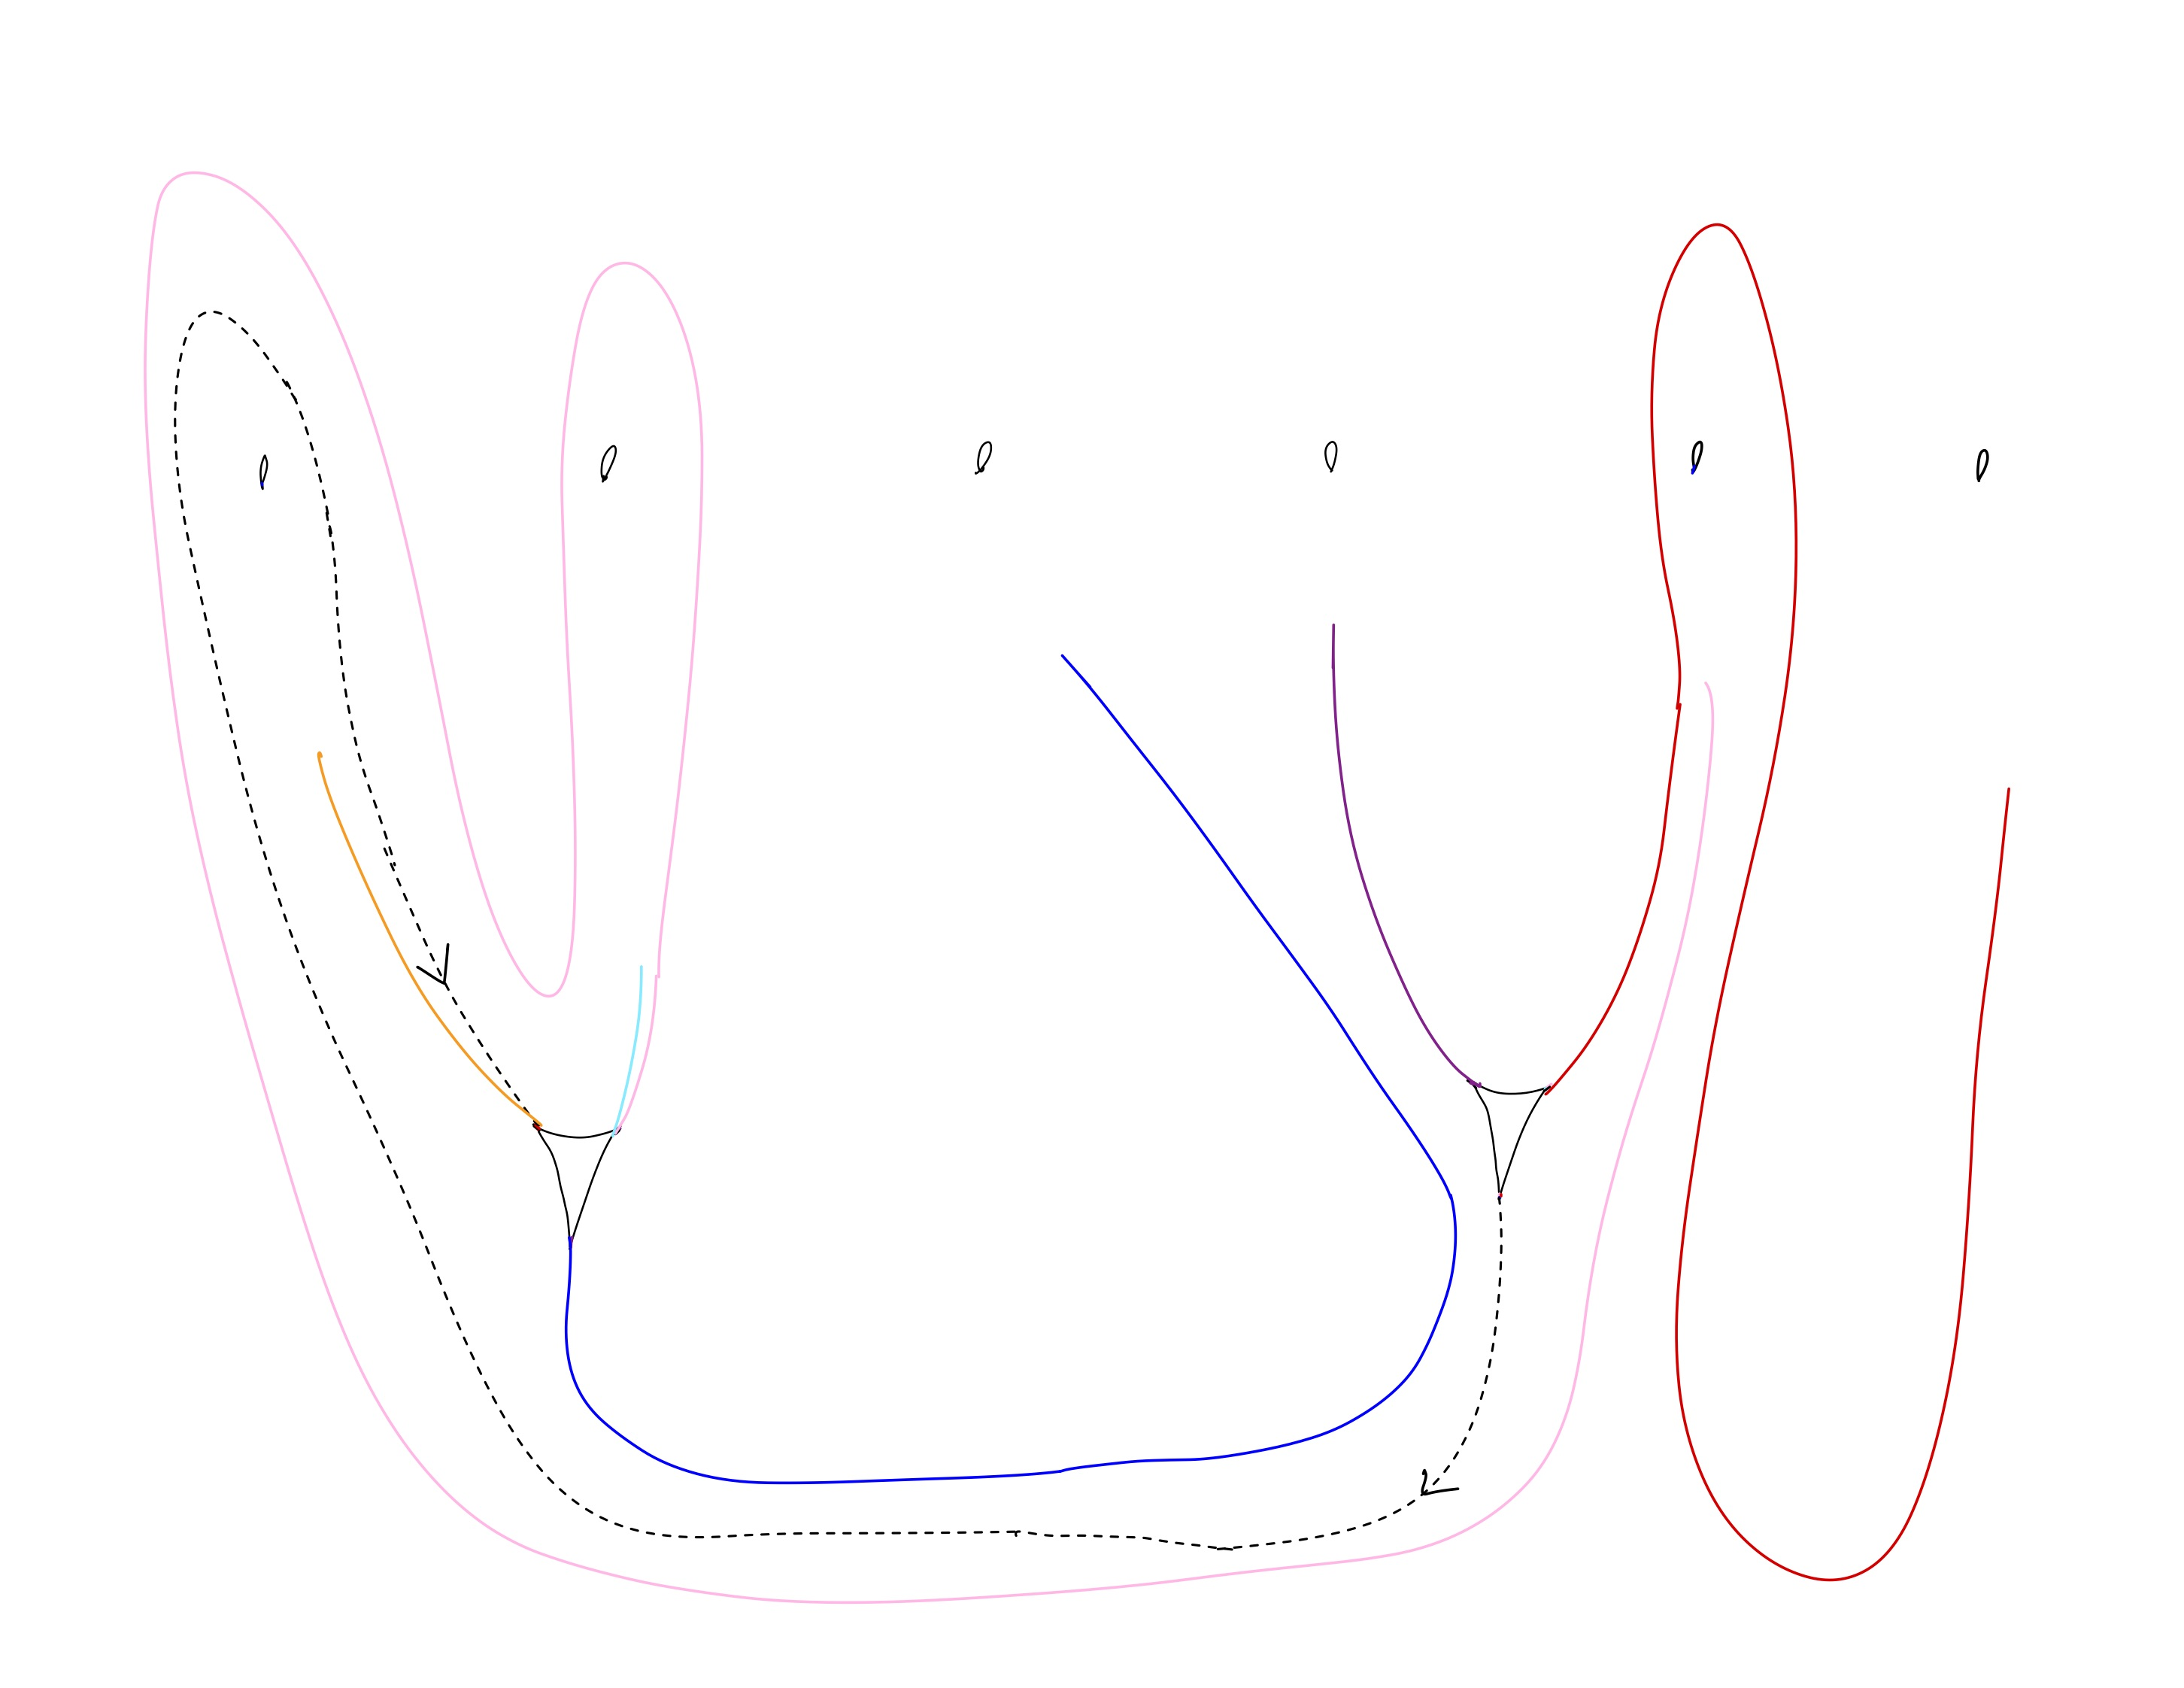
\includegraphics[width=\linewidth]{figures_case_analysis/track17_case_analysis/Boke-02.jpg}
    \caption{Boke2}
    \label{fig:Boke2}
\end{figure}

\begin{figure}[ht]
    \centering
    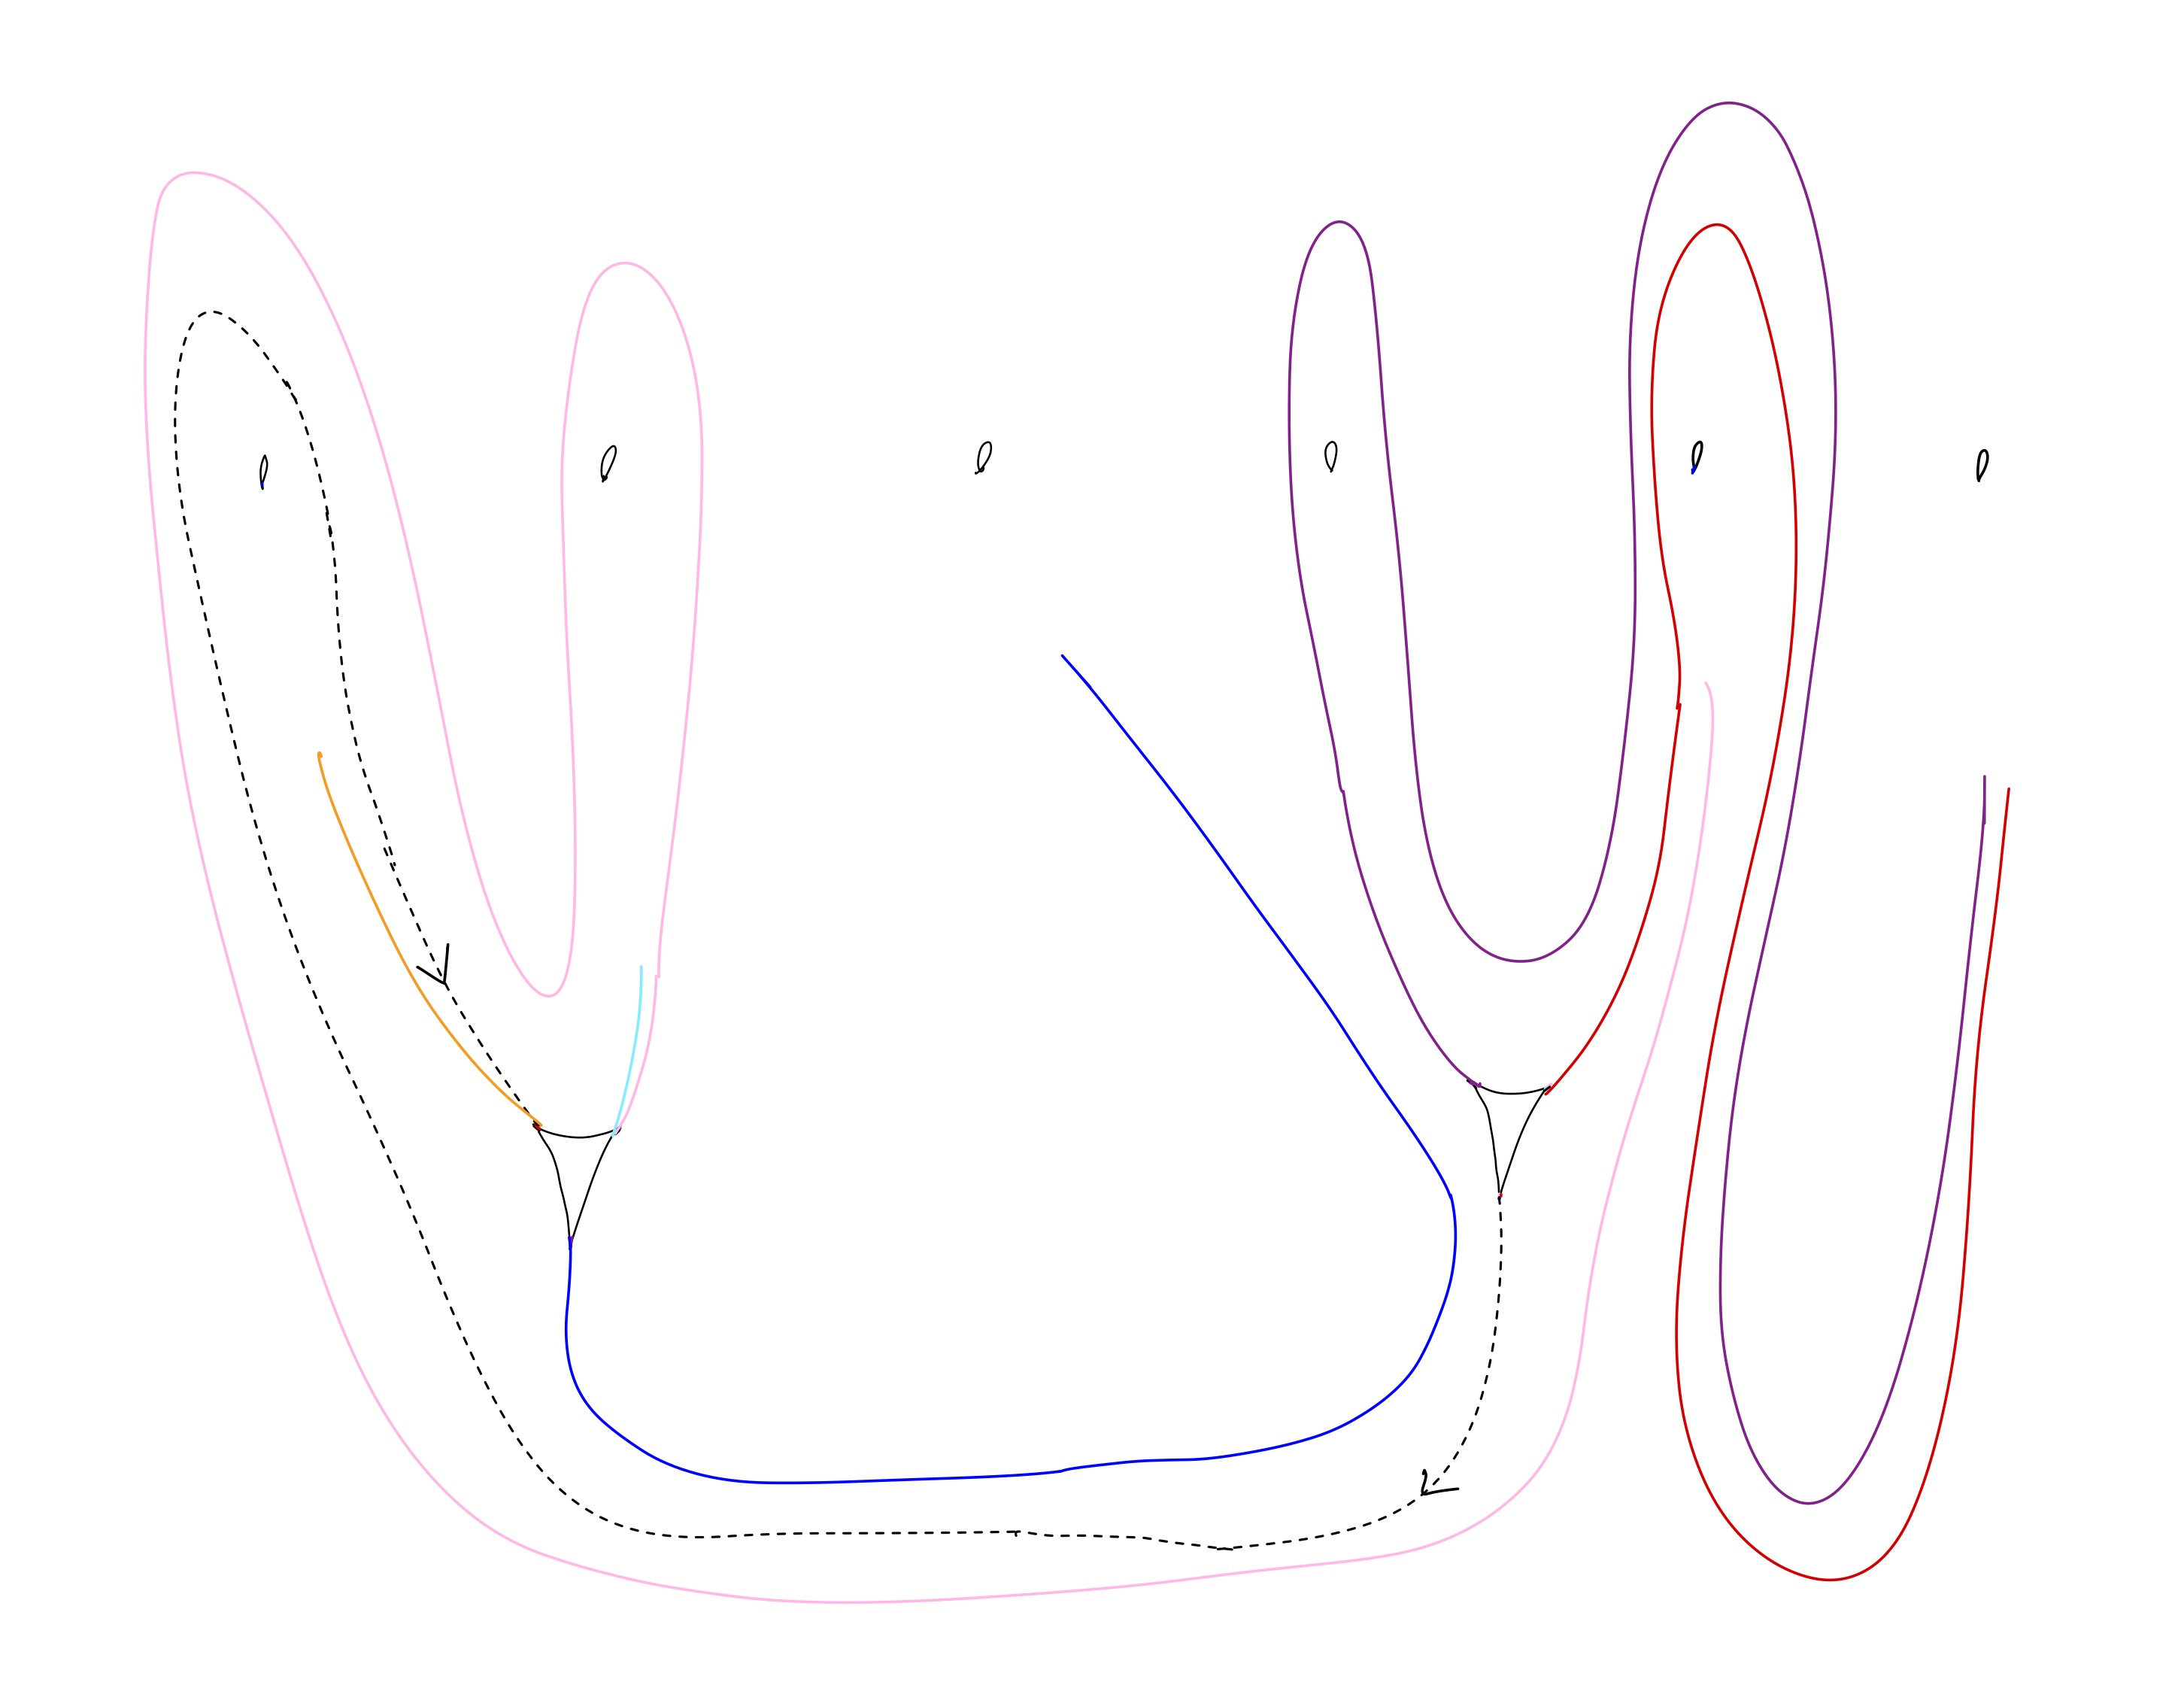
\includegraphics[width=\linewidth]{figures_case_analysis/track17_case_analysis/Boke-03.jpg}
    \caption{Boke3}
    \label{fig:Boke3}
\end{figure}

\begin{figure}[ht]
    \centering
    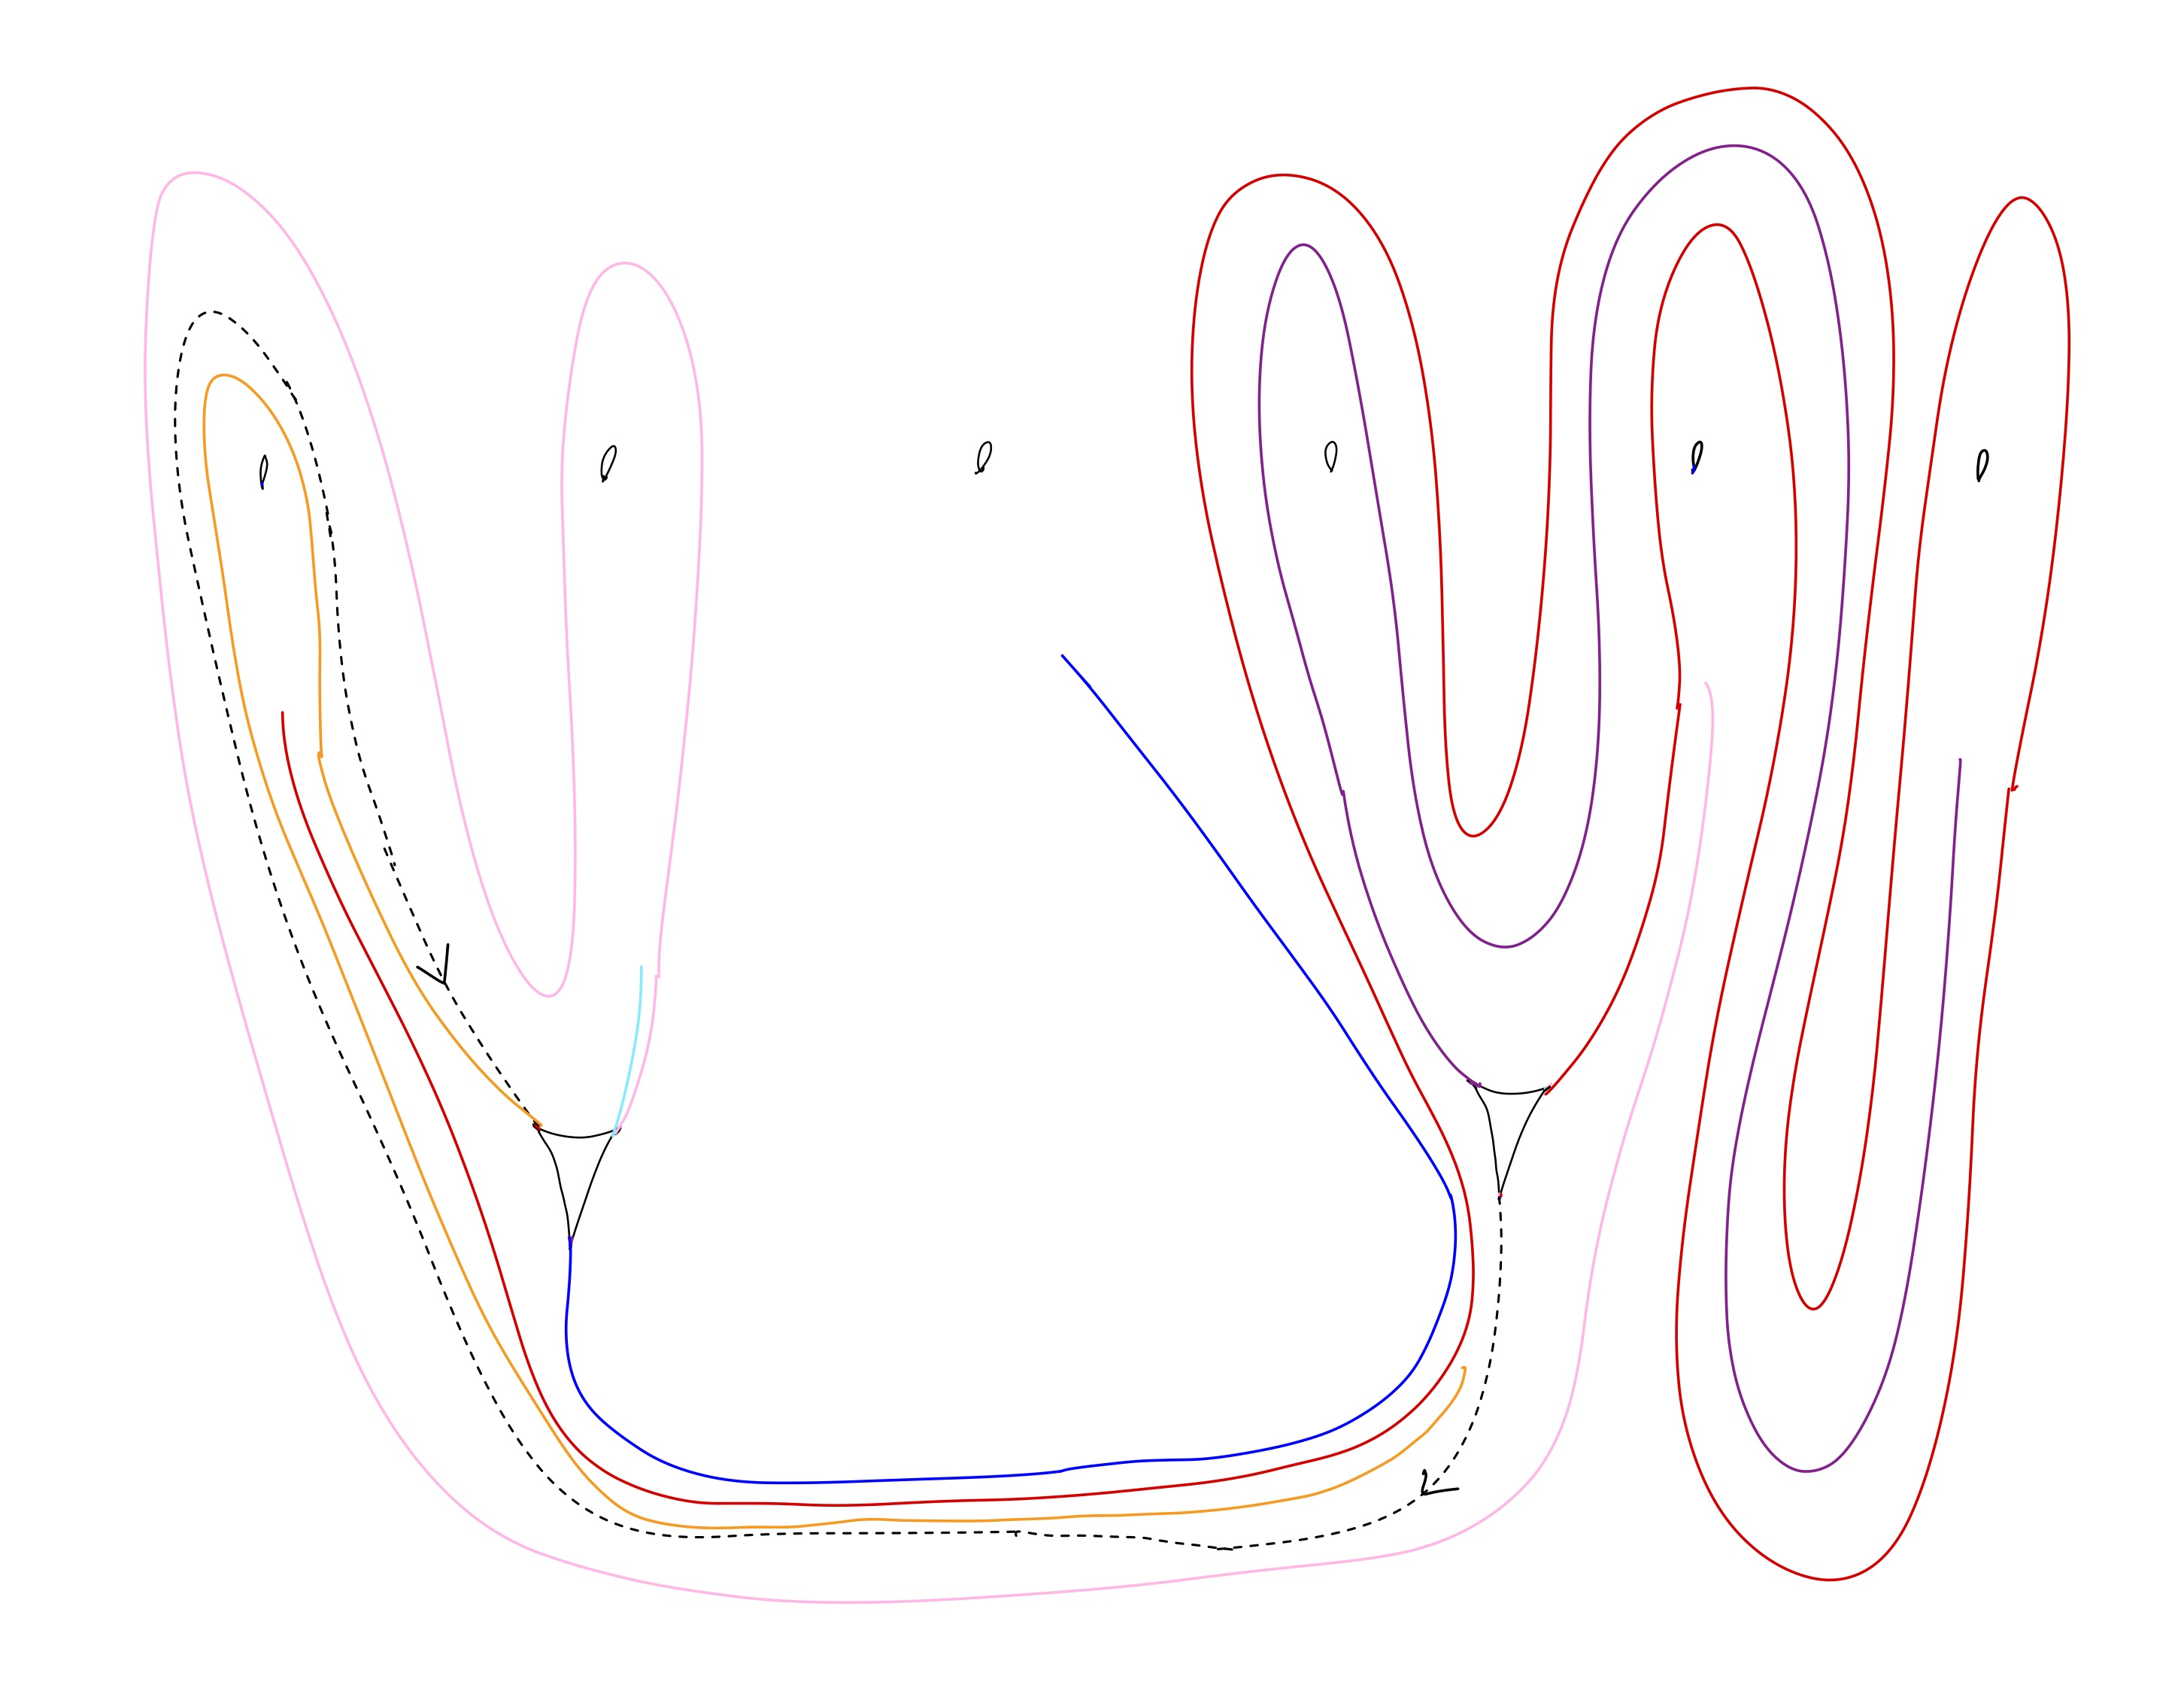
\includegraphics[width=\linewidth]{figures_case_analysis/track17_case_analysis/Boke-04.jpg}
    \caption{Boke4}
    \label{fig:Boke4}
\end{figure}

\begin{figure}[ht]
    \centering
    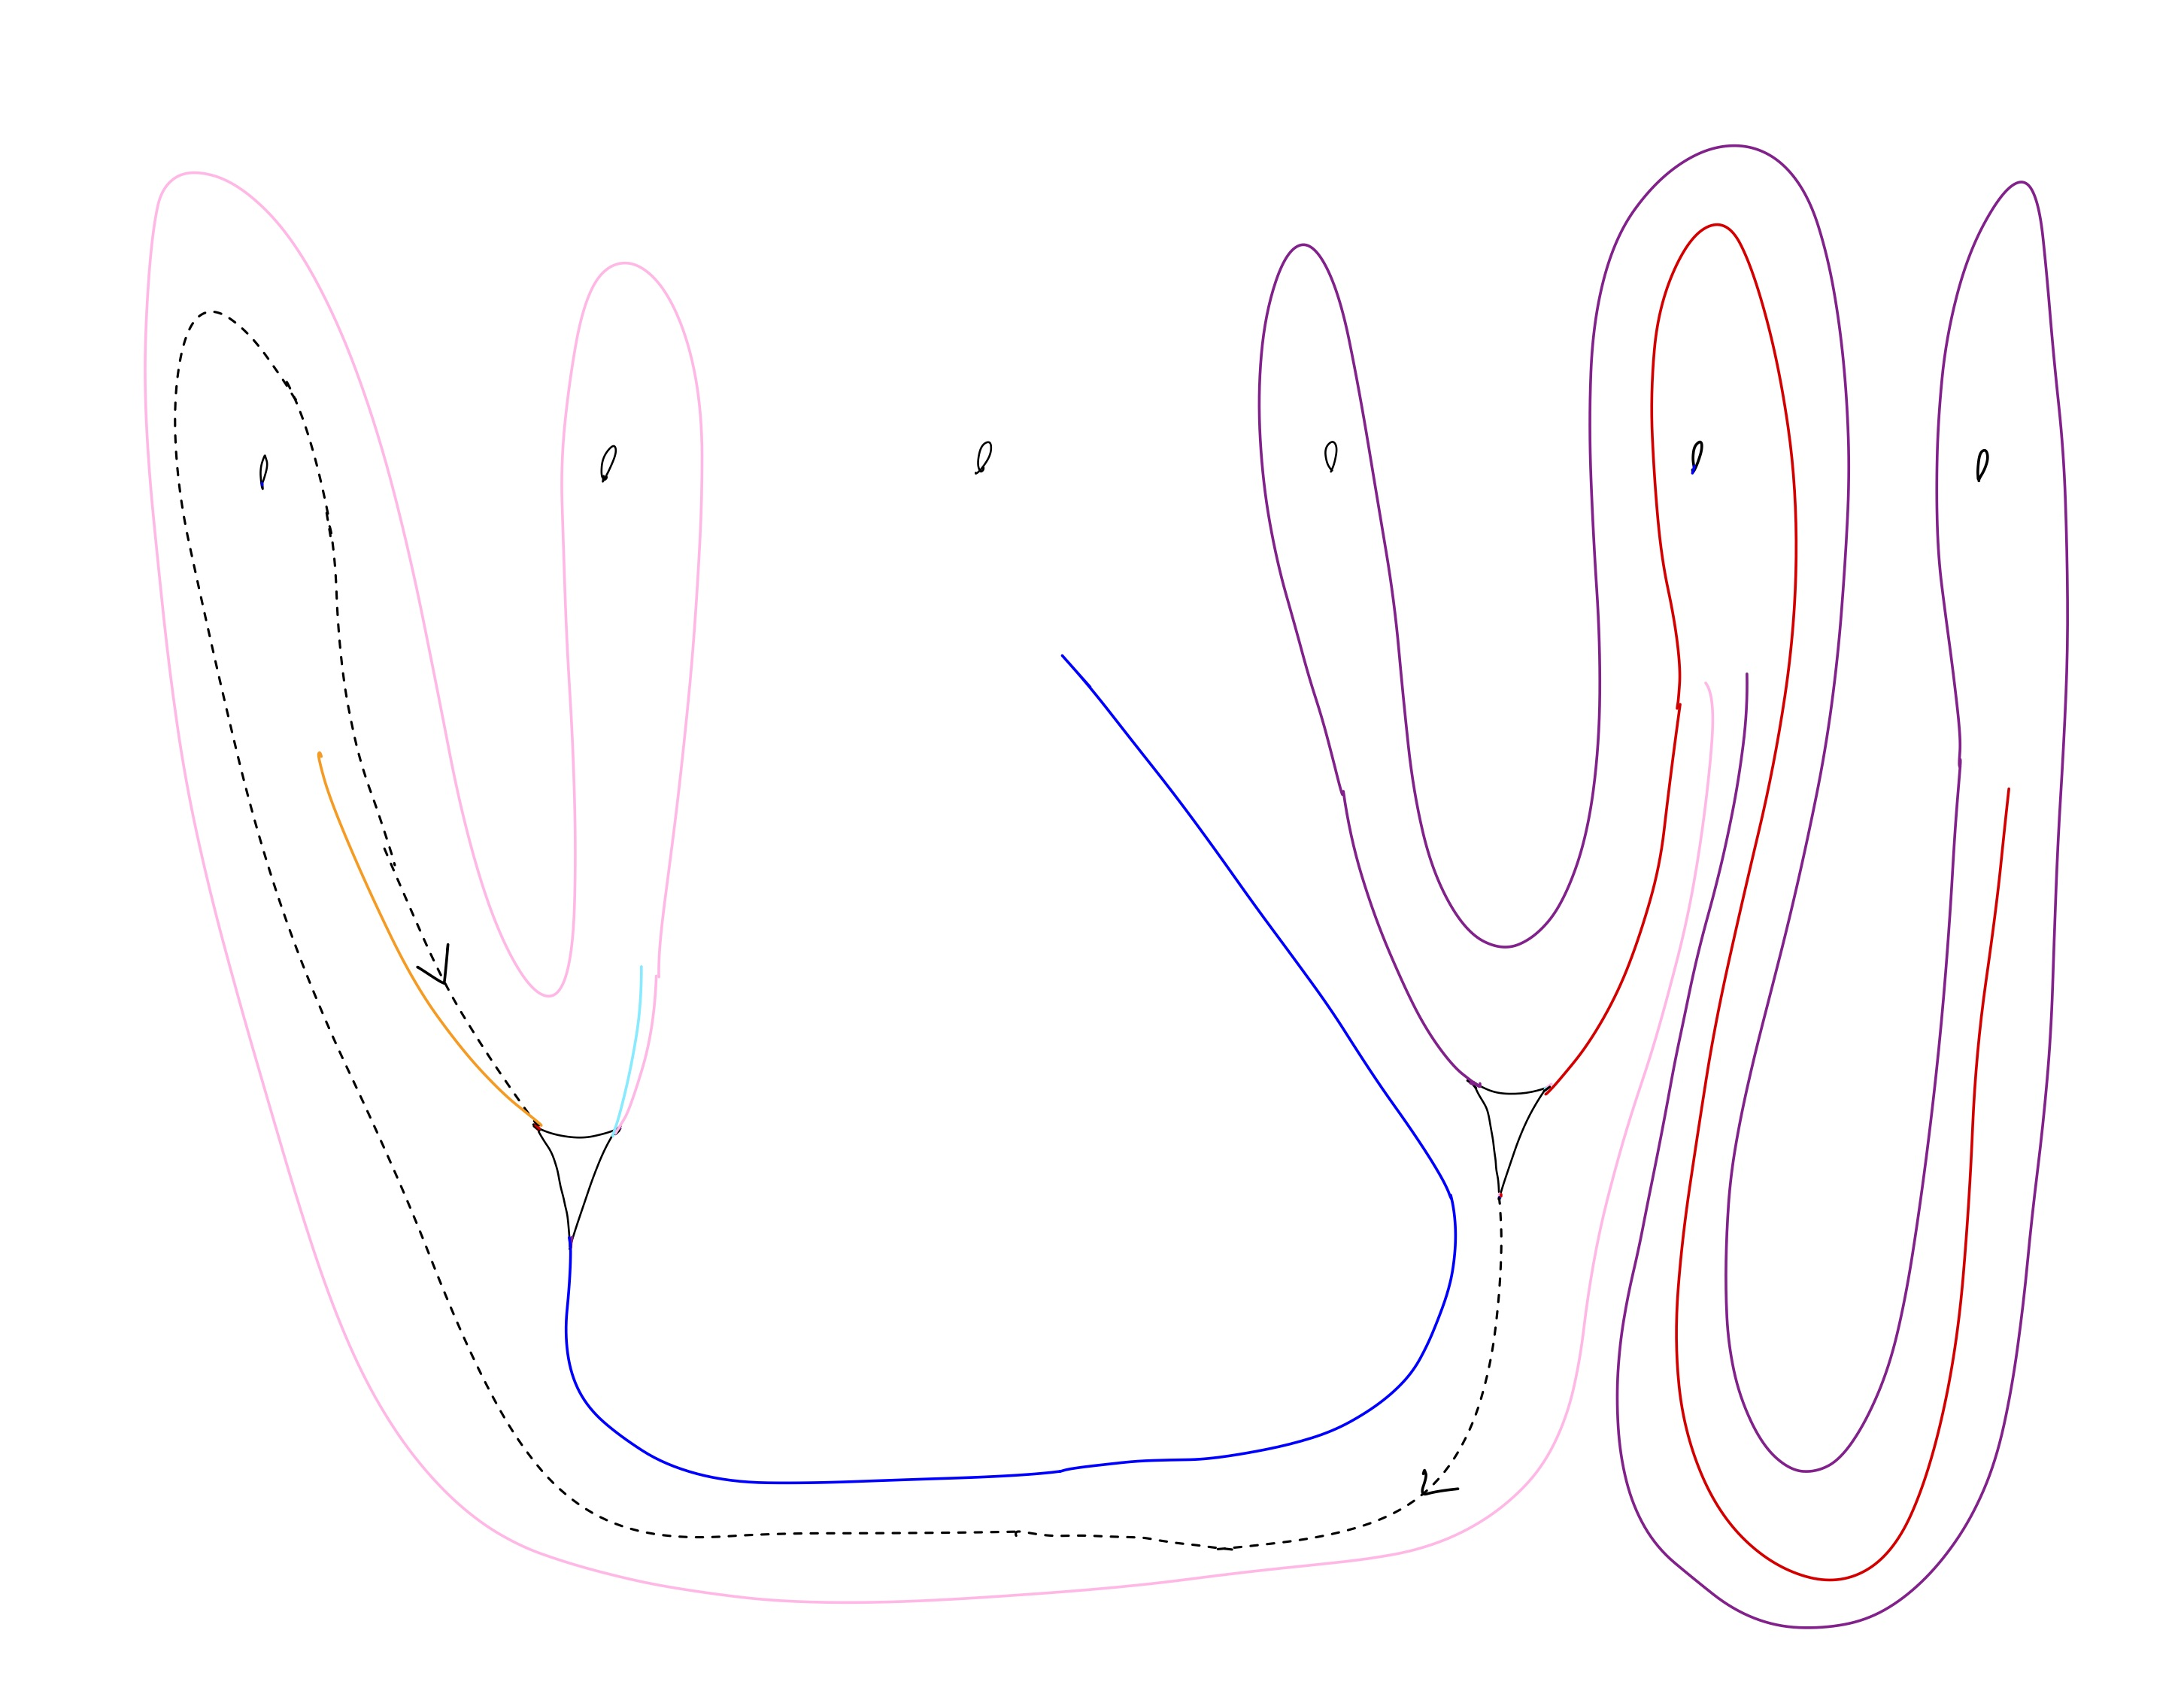
\includegraphics[width=\linewidth]{figures_case_analysis/track17_case_analysis/Boke-05.jpg}
    \caption{Boke5}
    \label{fig:Boke5}
\end{figure}

\begin{figure}[ht]
    \centering
    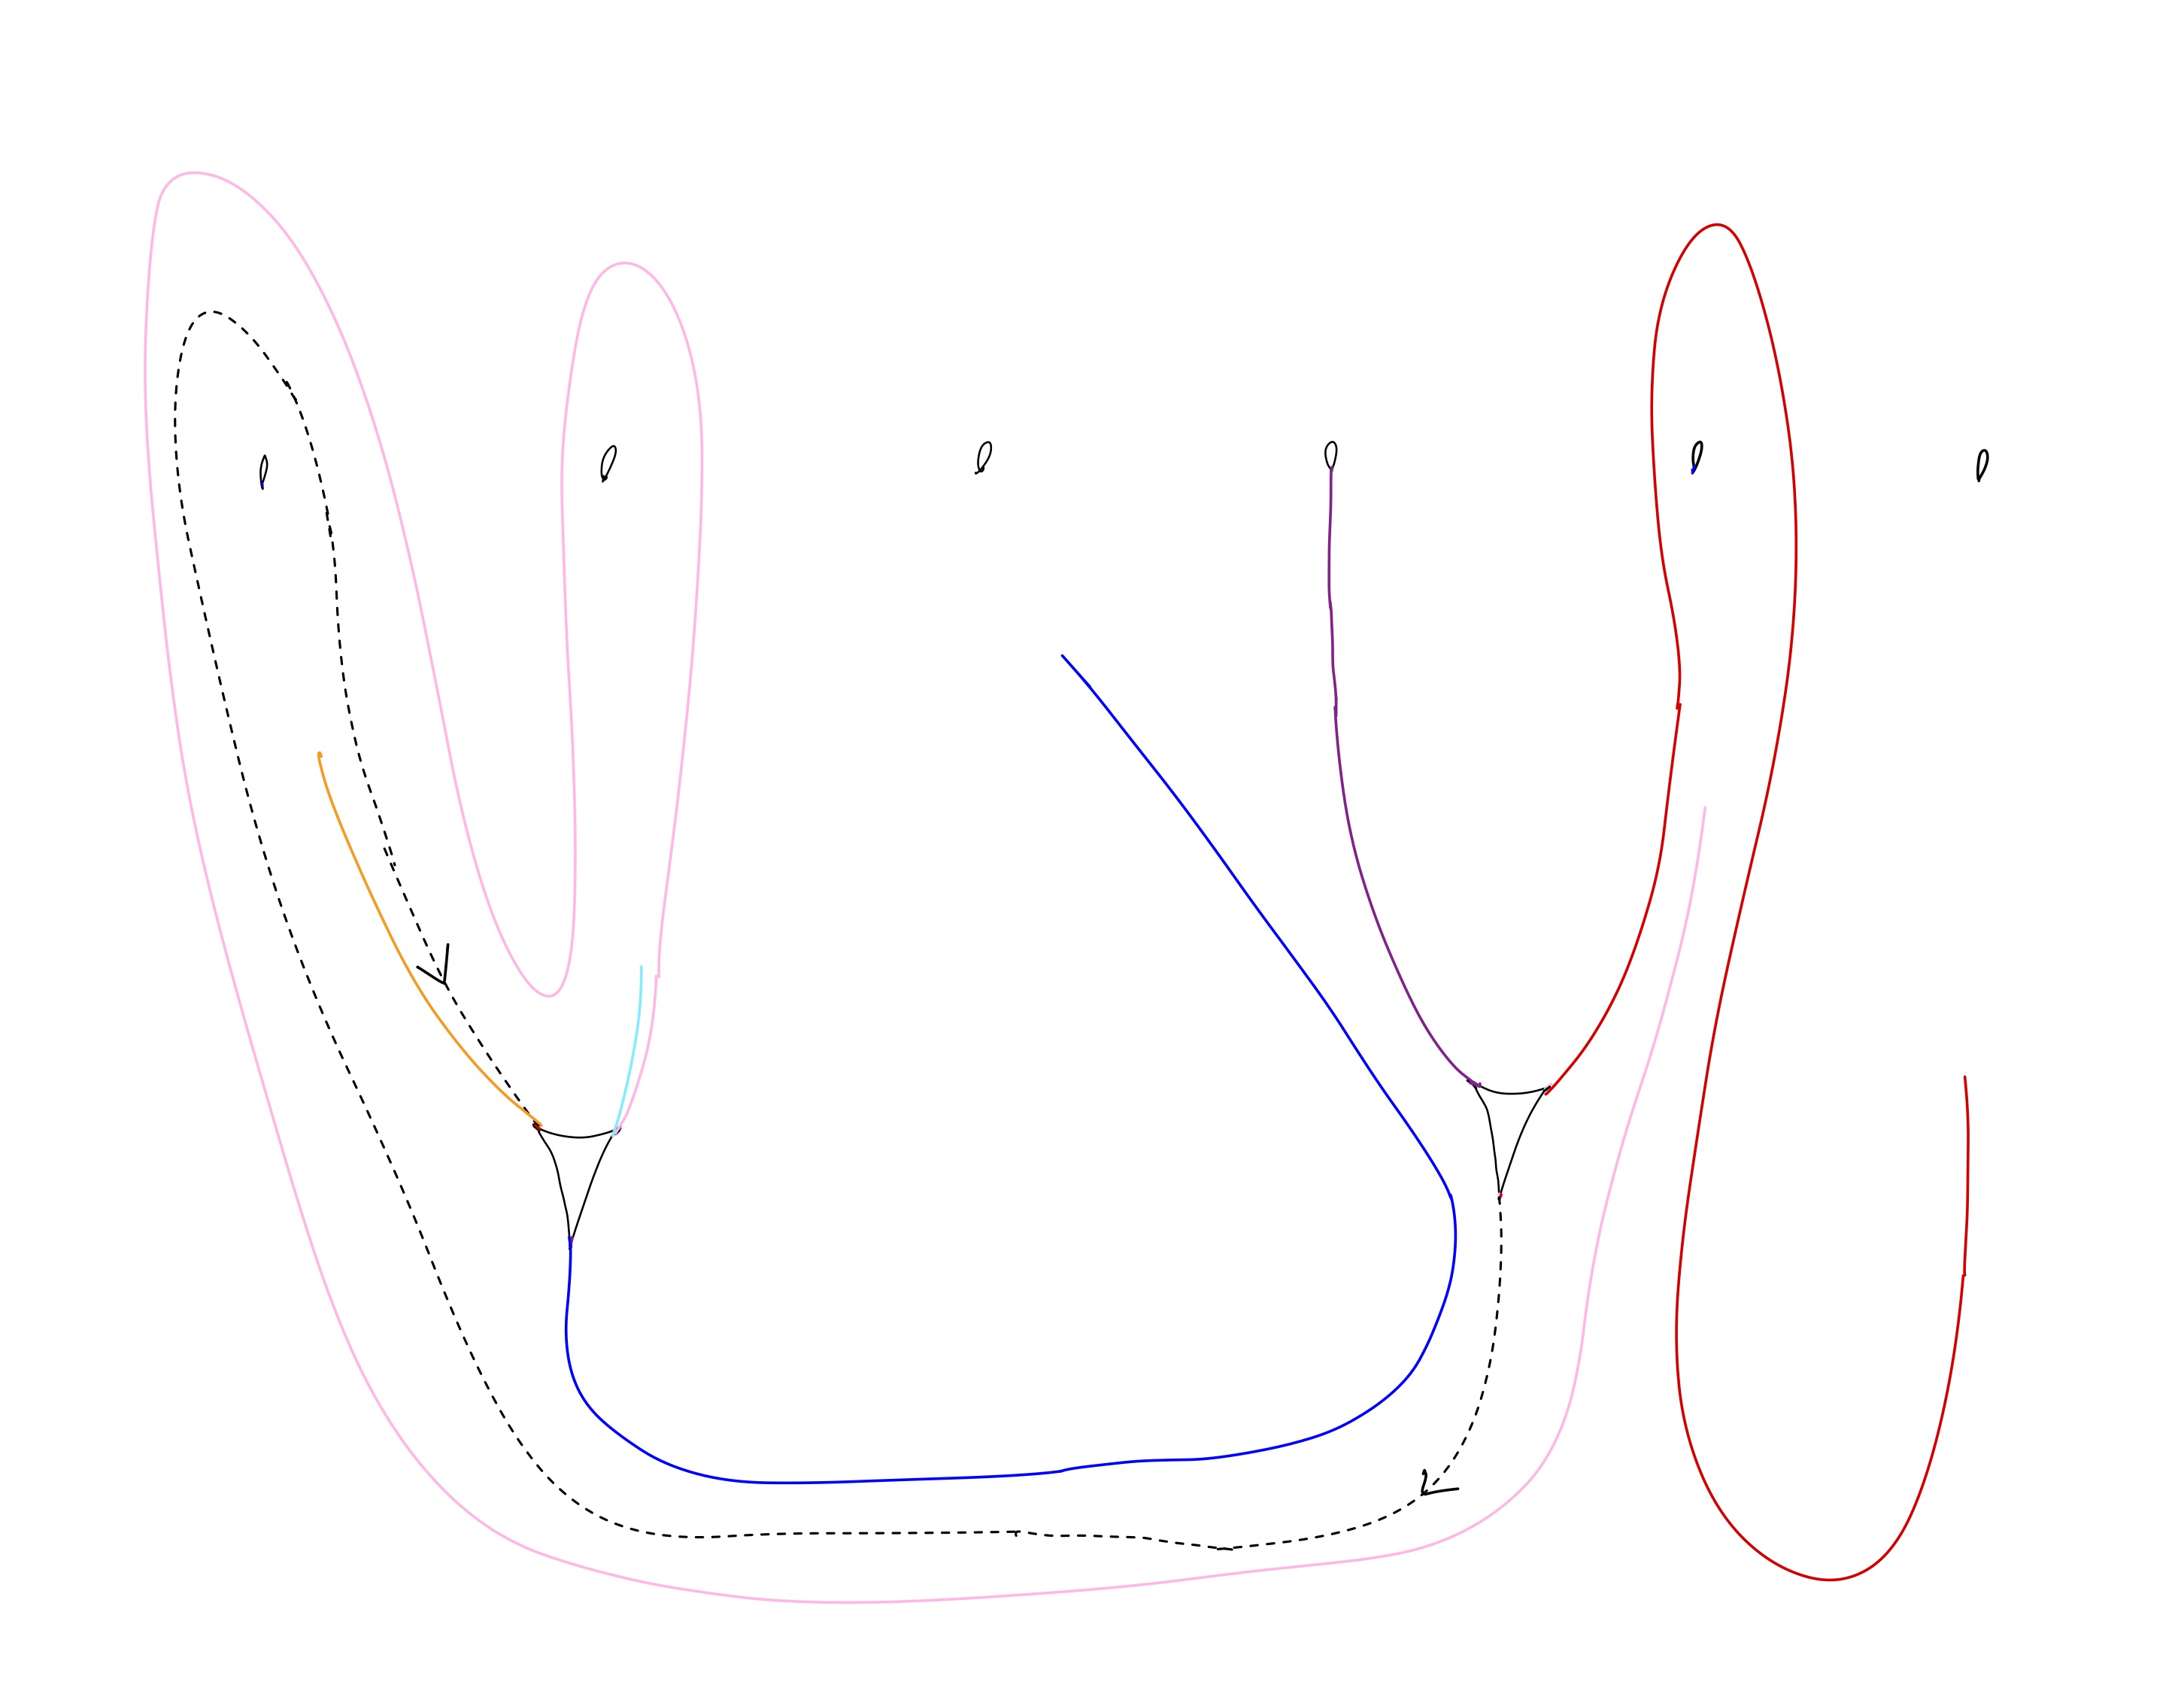
\includegraphics[width=\linewidth]{figures_case_analysis/track17_case_analysis/Boke-06.jpg}
    \caption{Boke6}
    \label{fig:Boke6}
\end{figure}

\begin{figure}[ht]
    \centering
    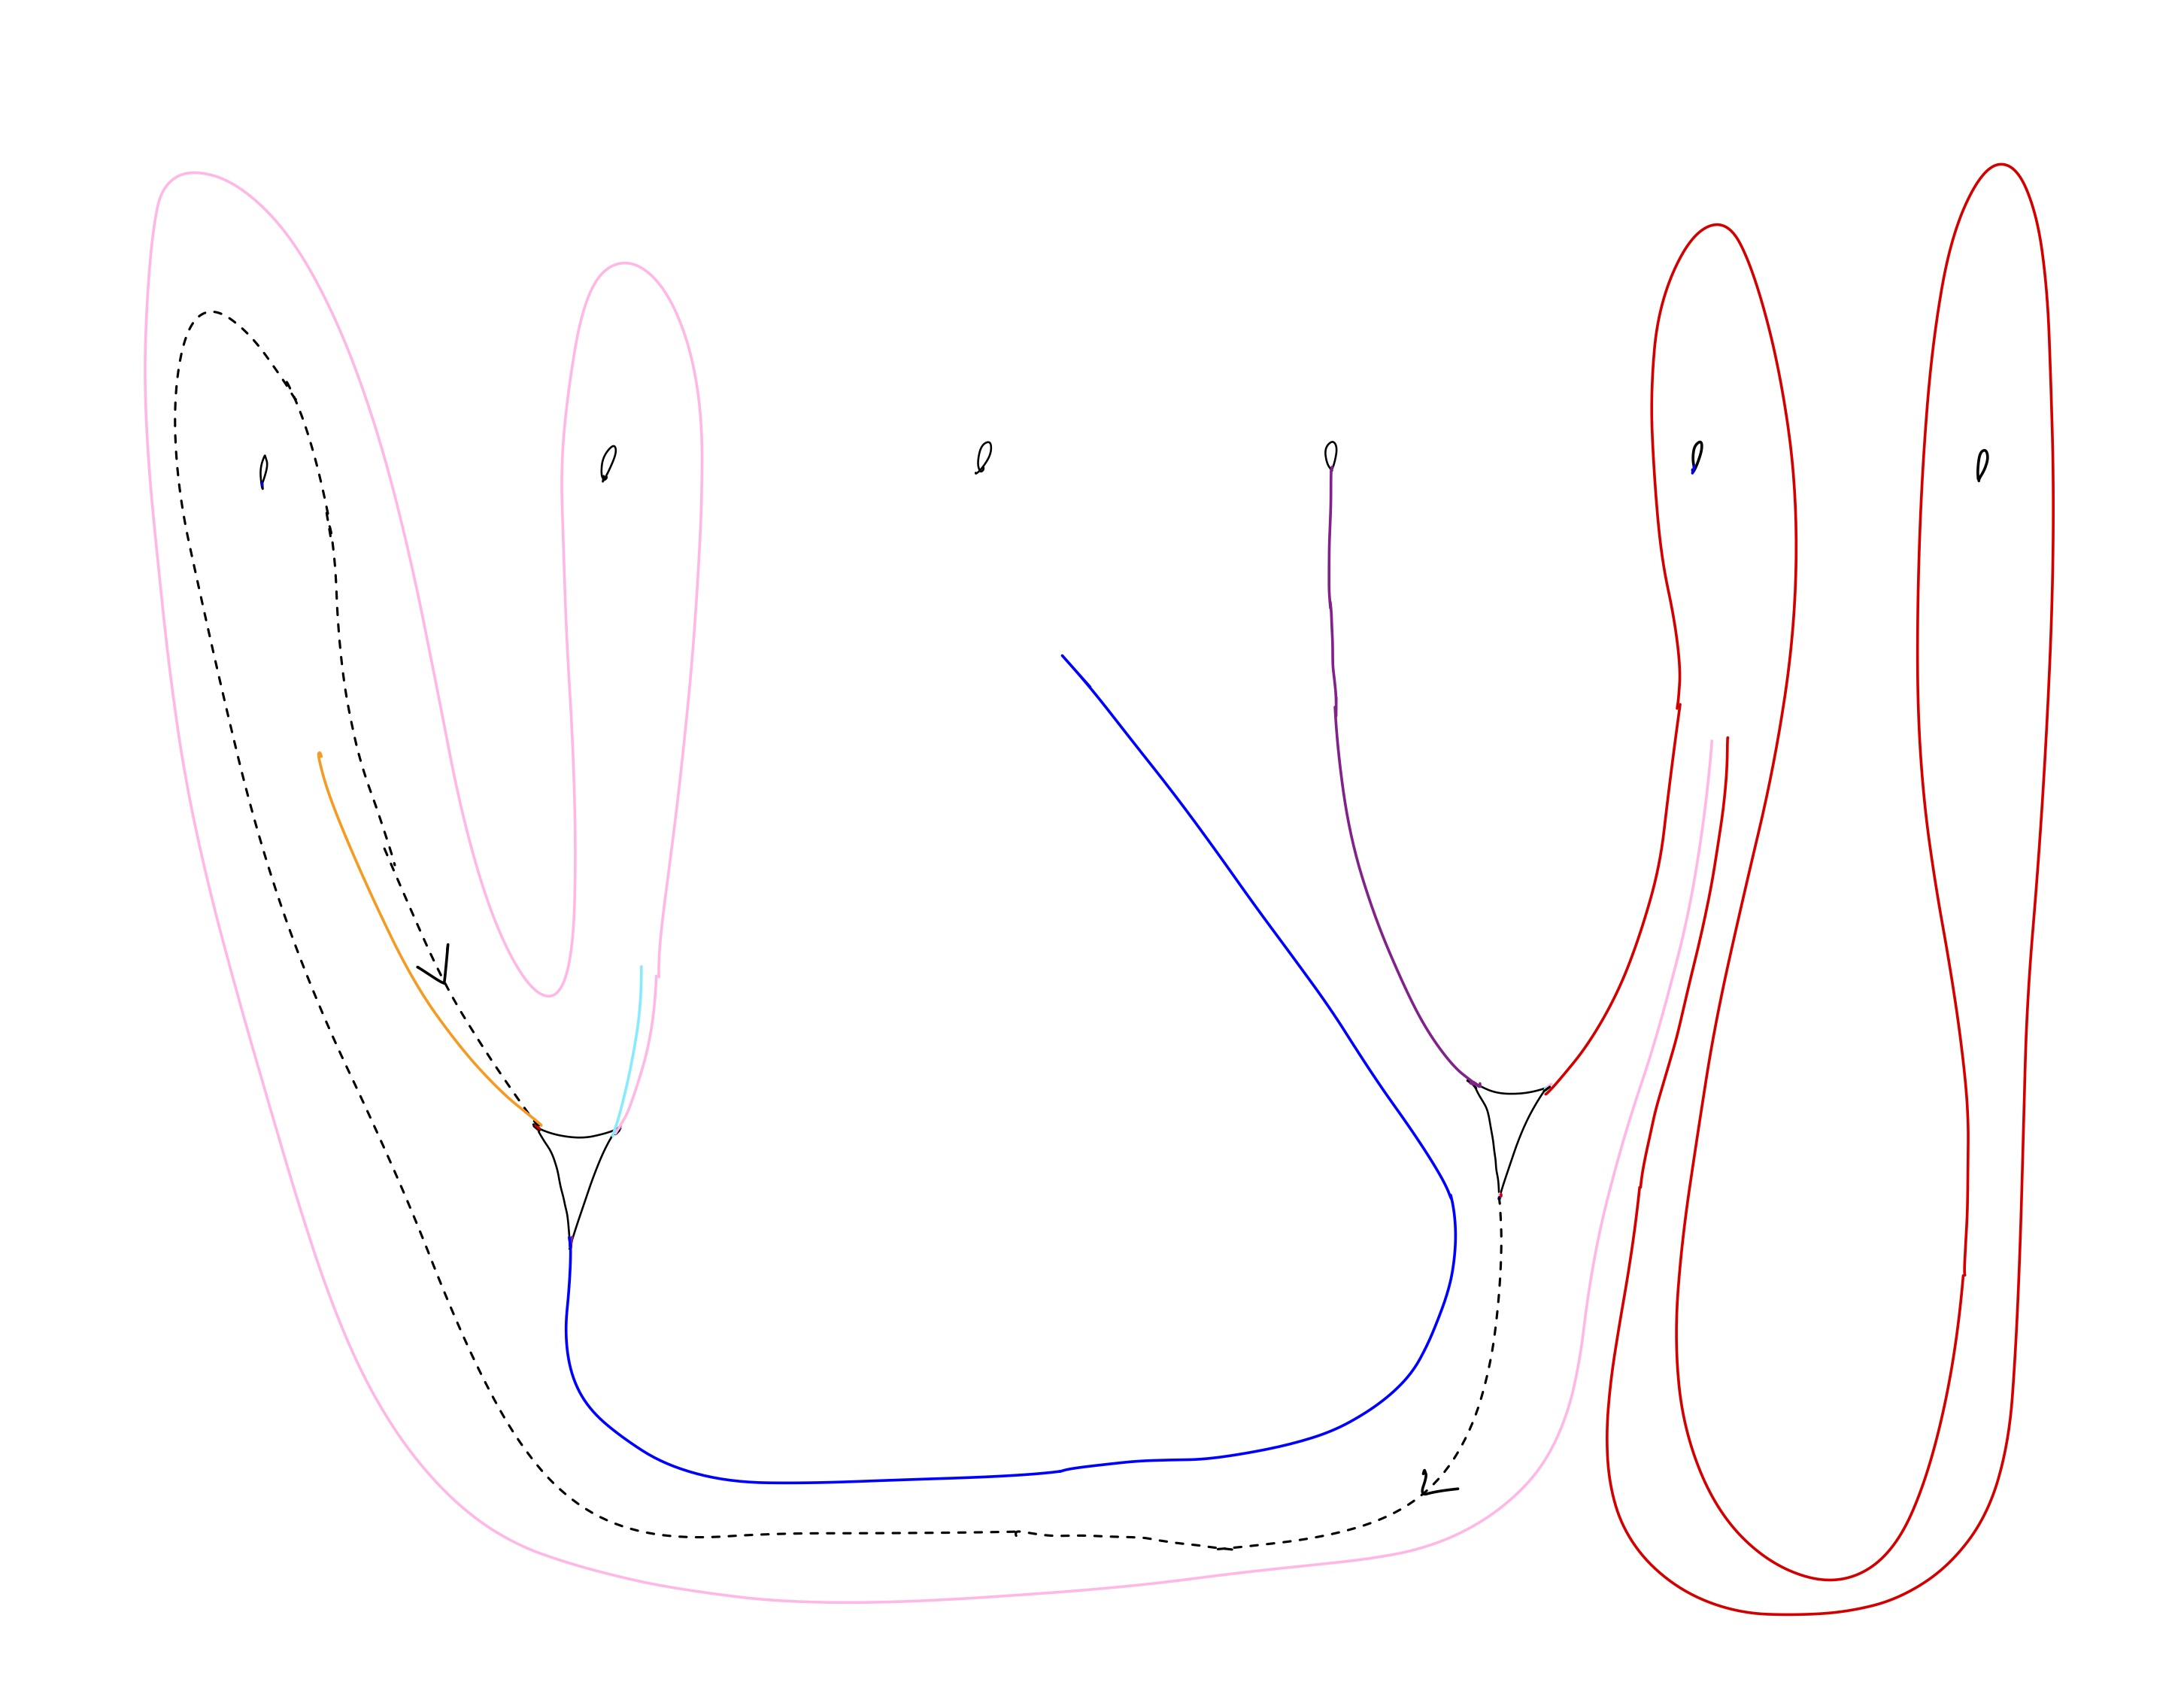
\includegraphics[width=\linewidth]{figures_case_analysis/track17_case_analysis/Boke-07.jpg}
    \caption{Boke7}
    \label{fig:Boke7}
\end{figure}

\begin{figure}[ht]
    \centering
    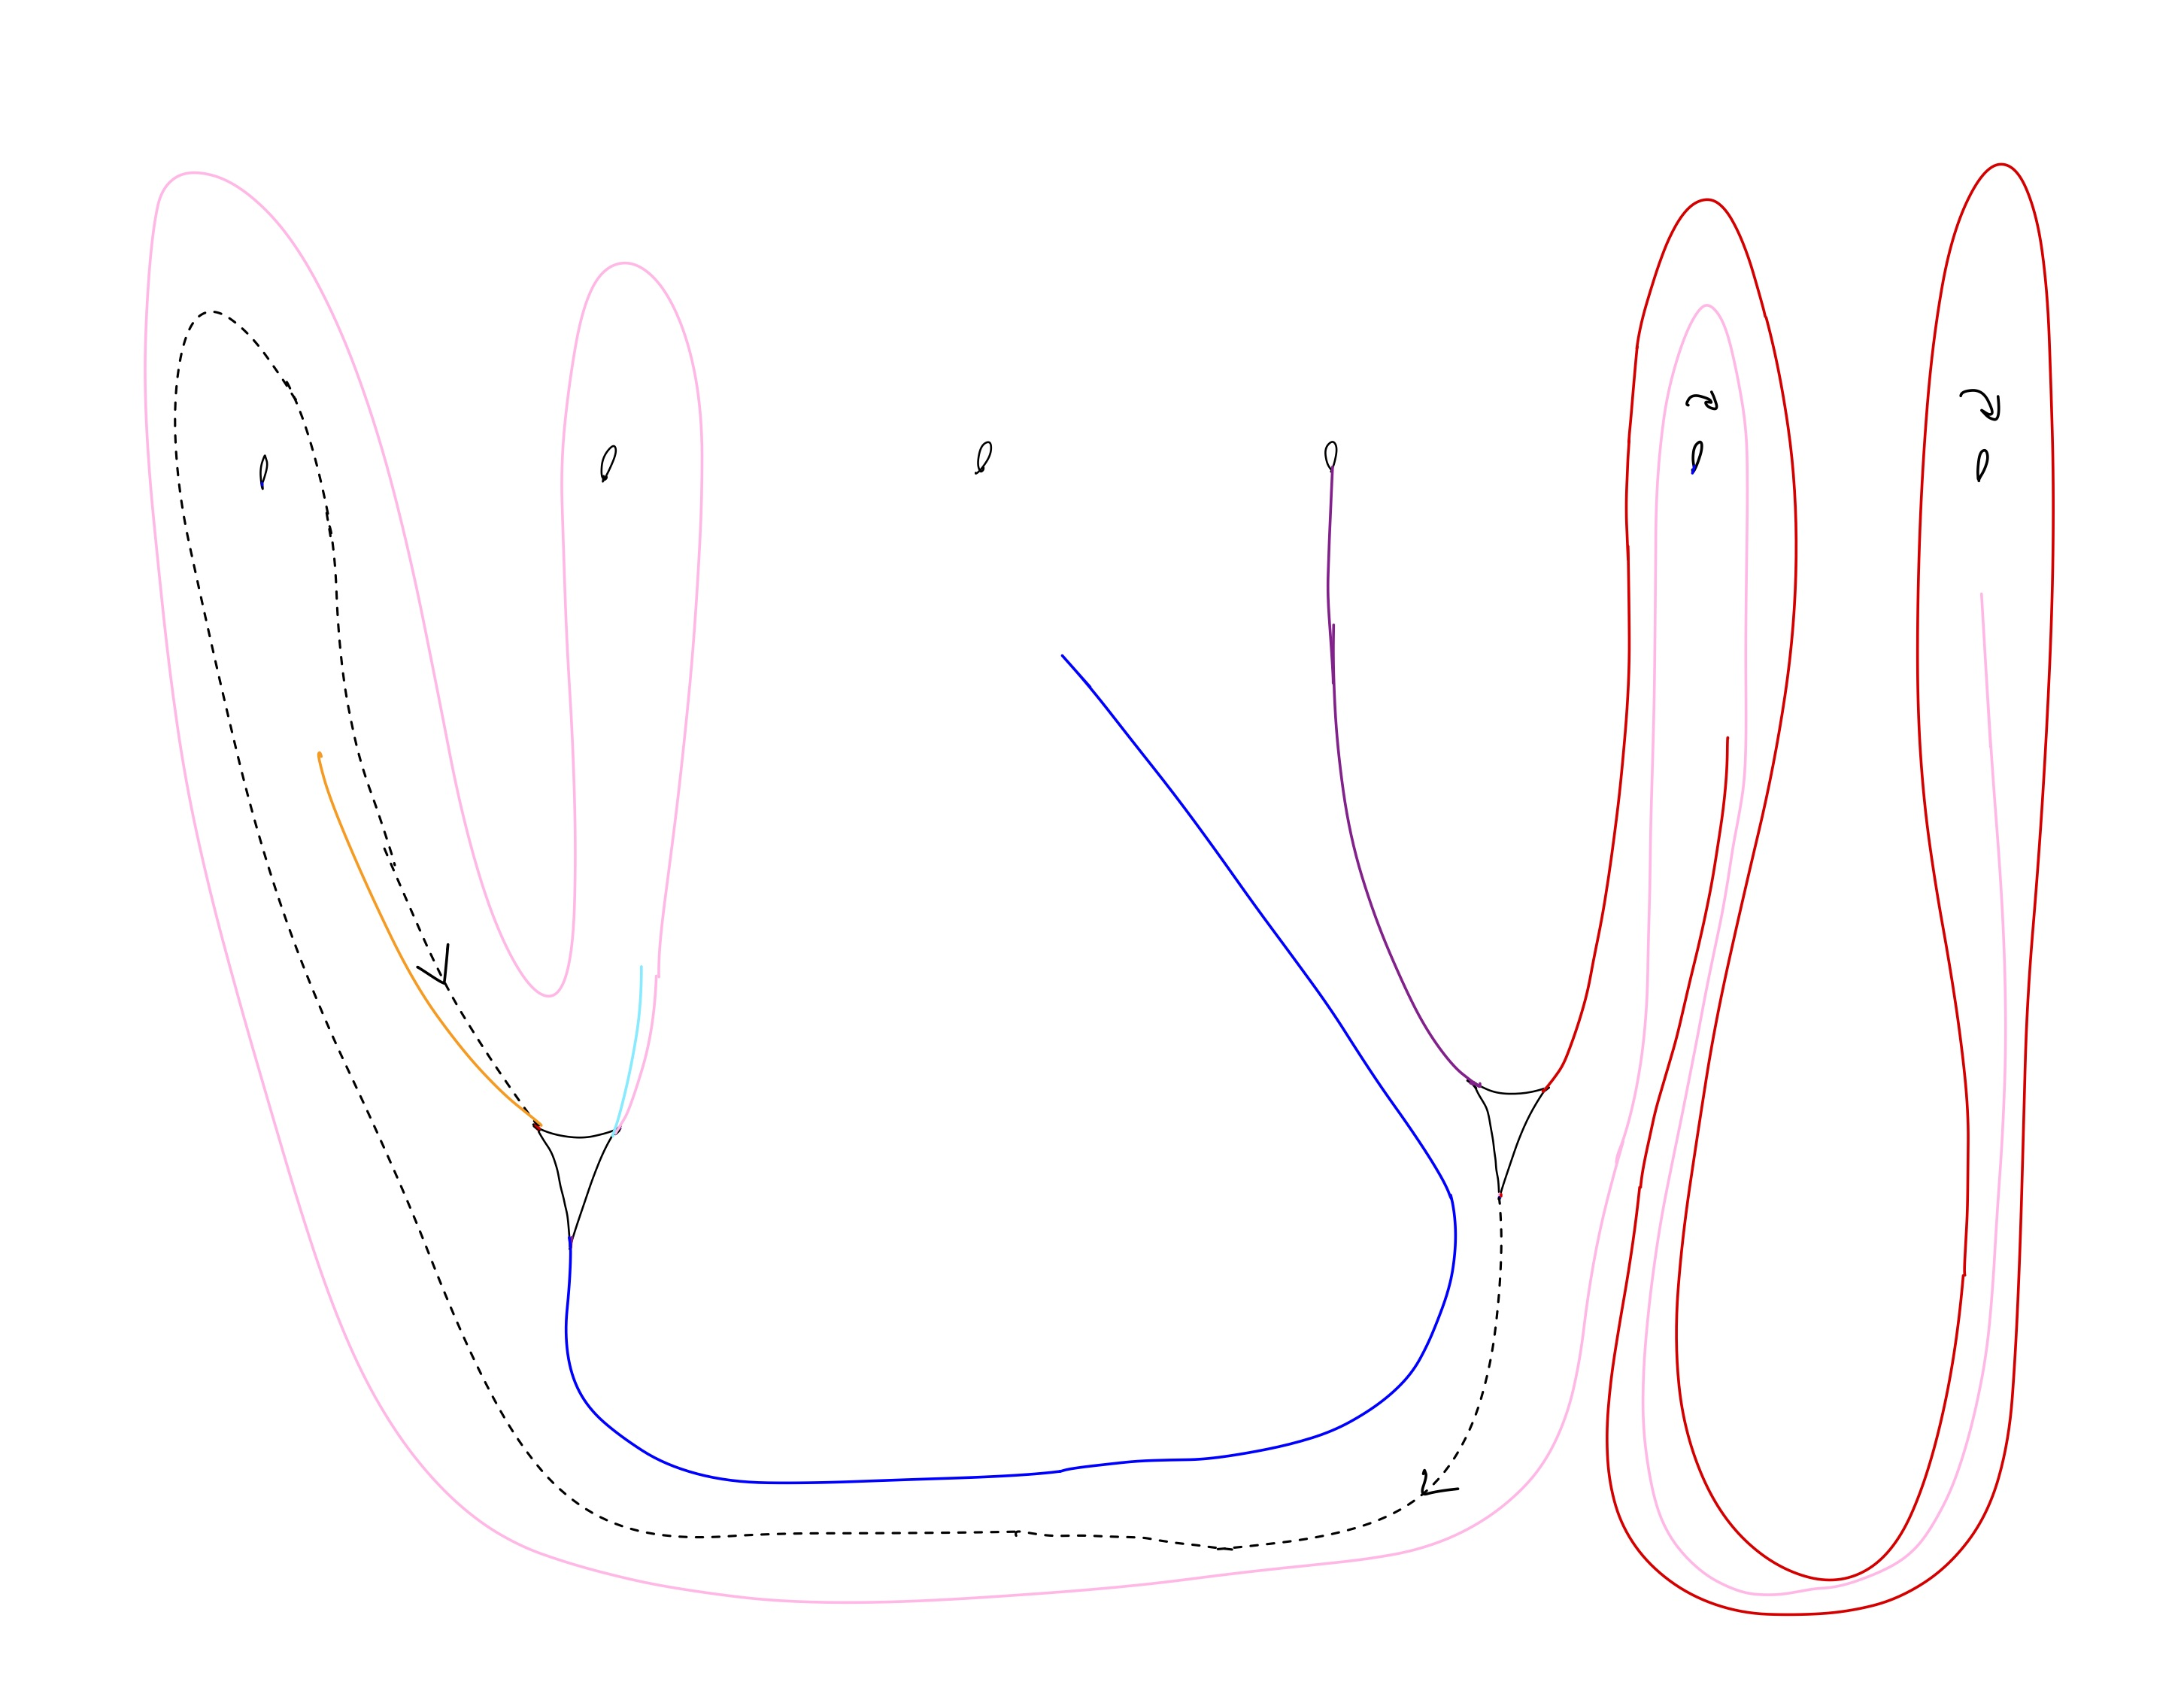
\includegraphics[width=\linewidth]{figures_case_analysis/track17_case_analysis/Boke-08.jpg}
    \caption{Boke8}
    \label{fig:Boke8}
\end{figure}

\begin{figure}[ht]
    \centering
    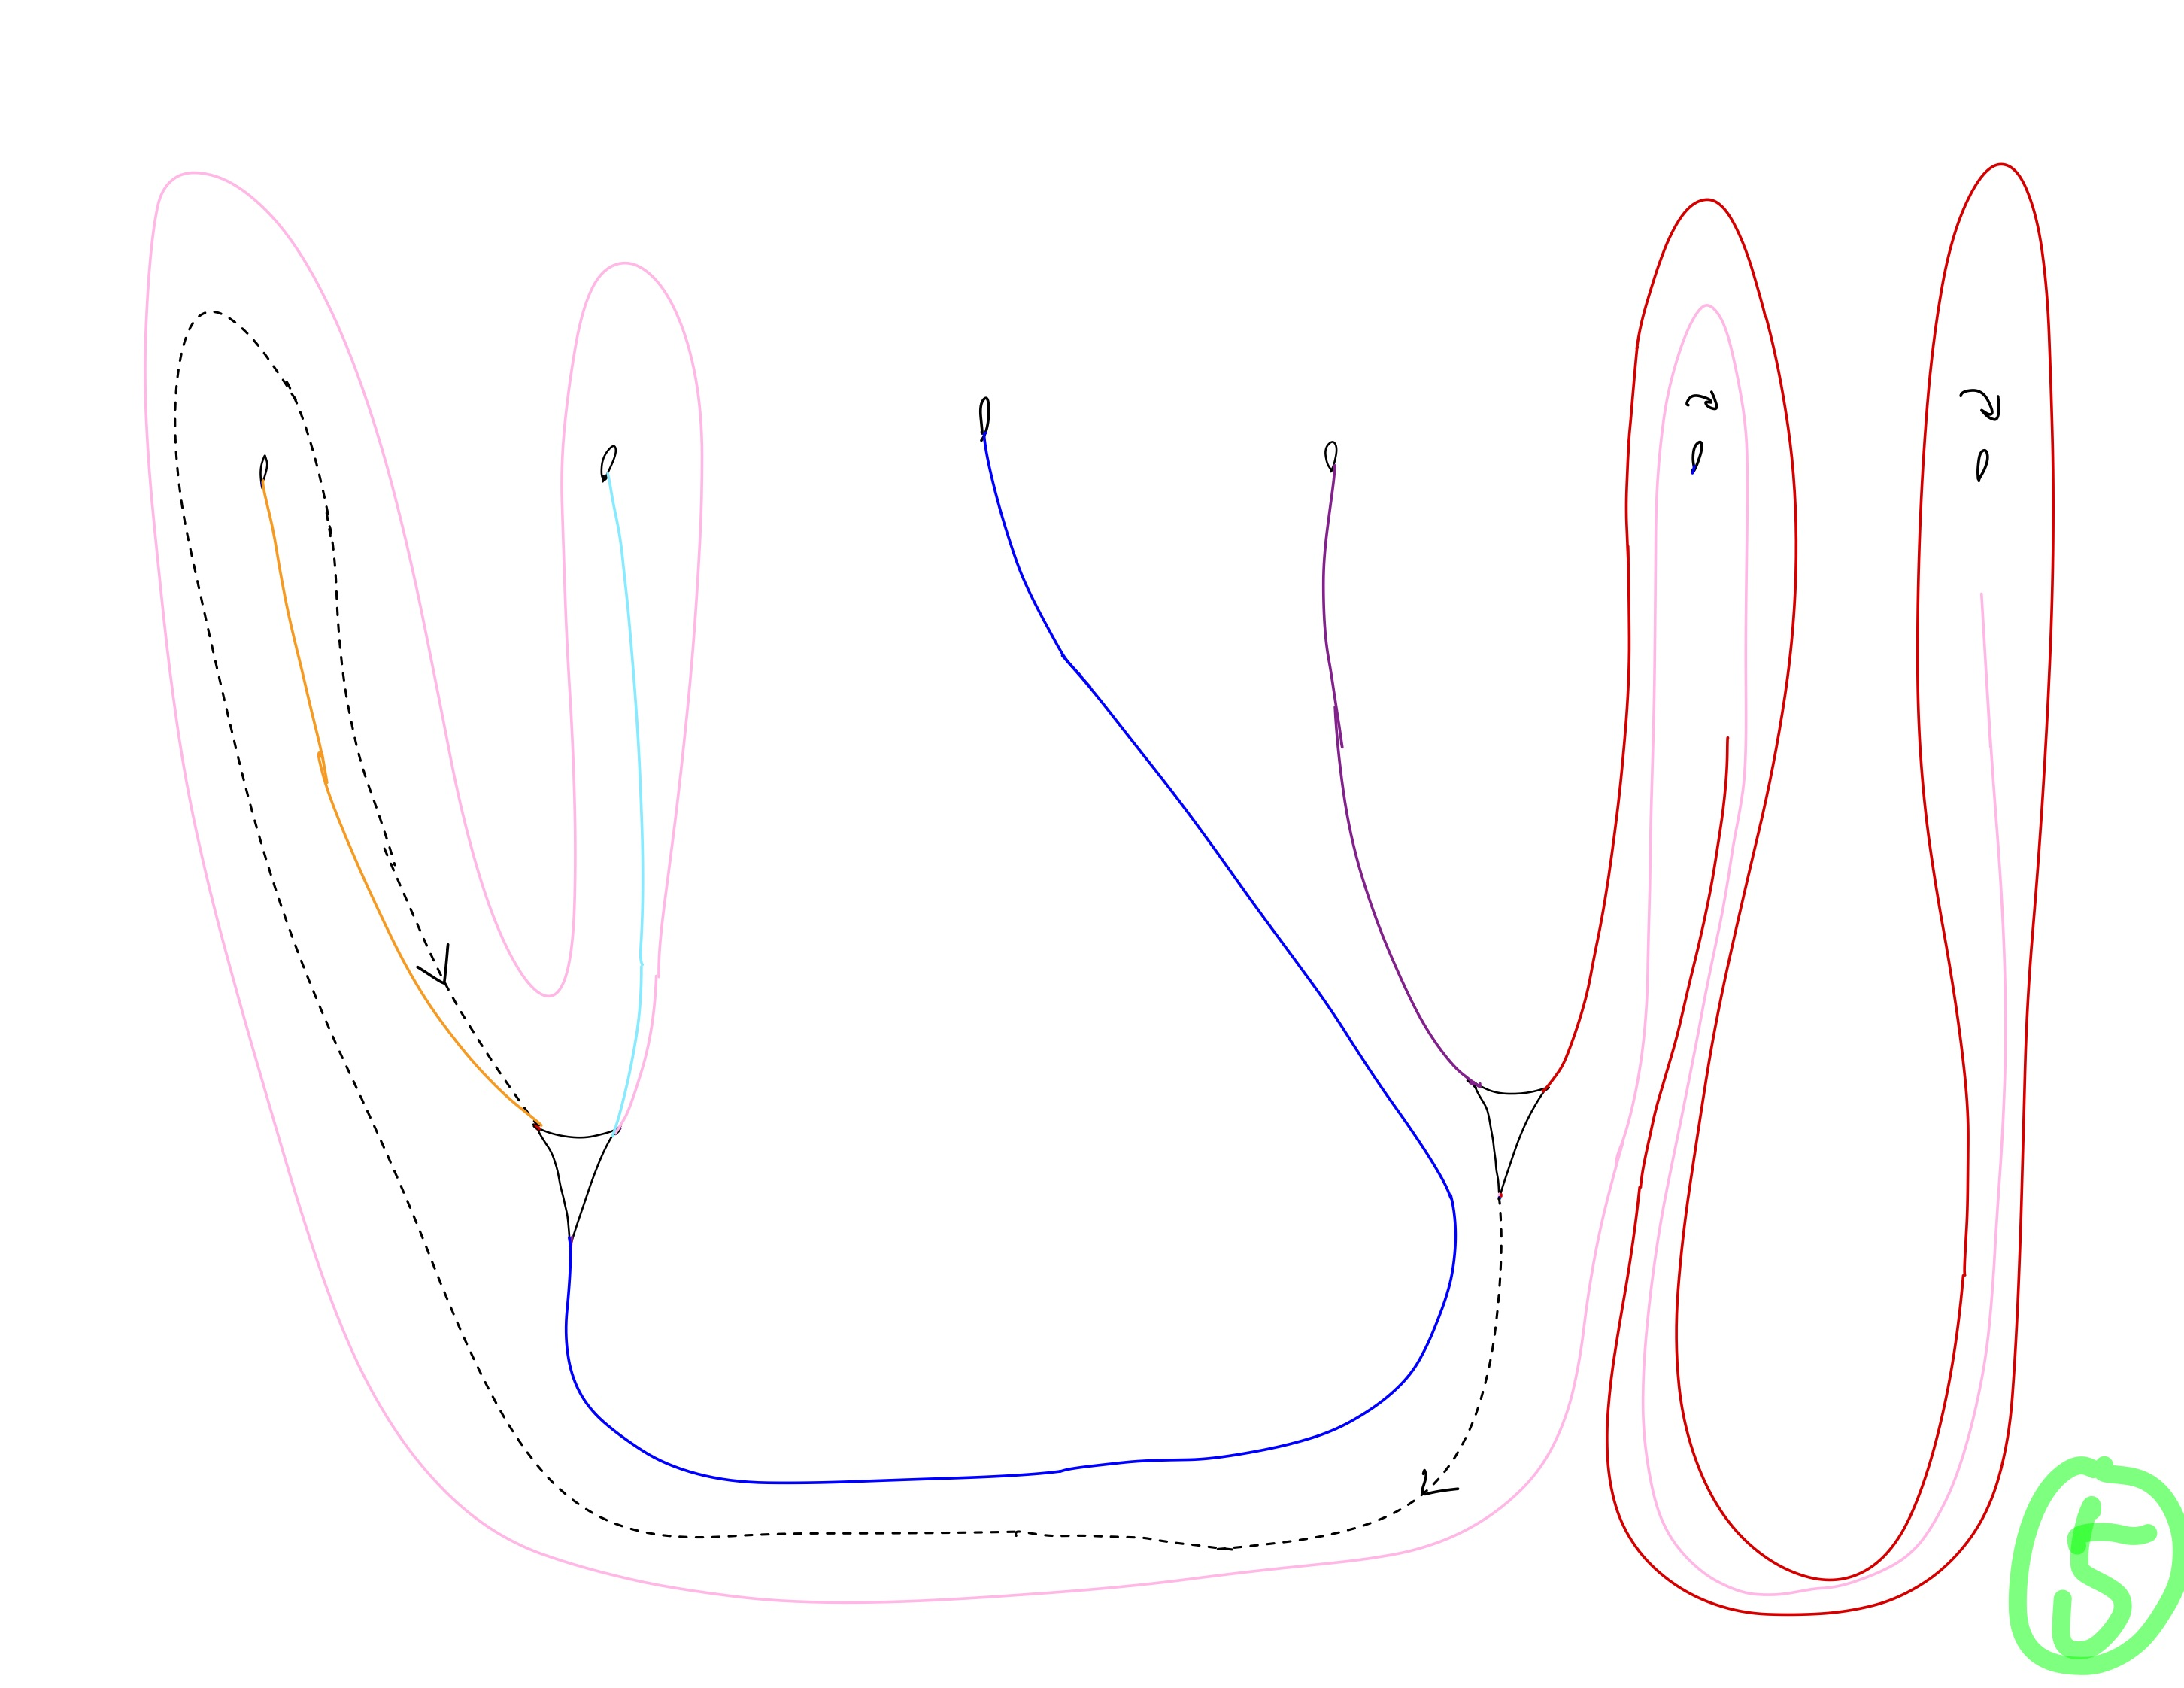
\includegraphics[width=\linewidth]{figures_case_analysis/track17_case_analysis/Boke-09.jpg}
    \caption{Boke9}
    \label{fig:Boke9}
\end{figure}

\begin{figure}[ht]
    \centering
    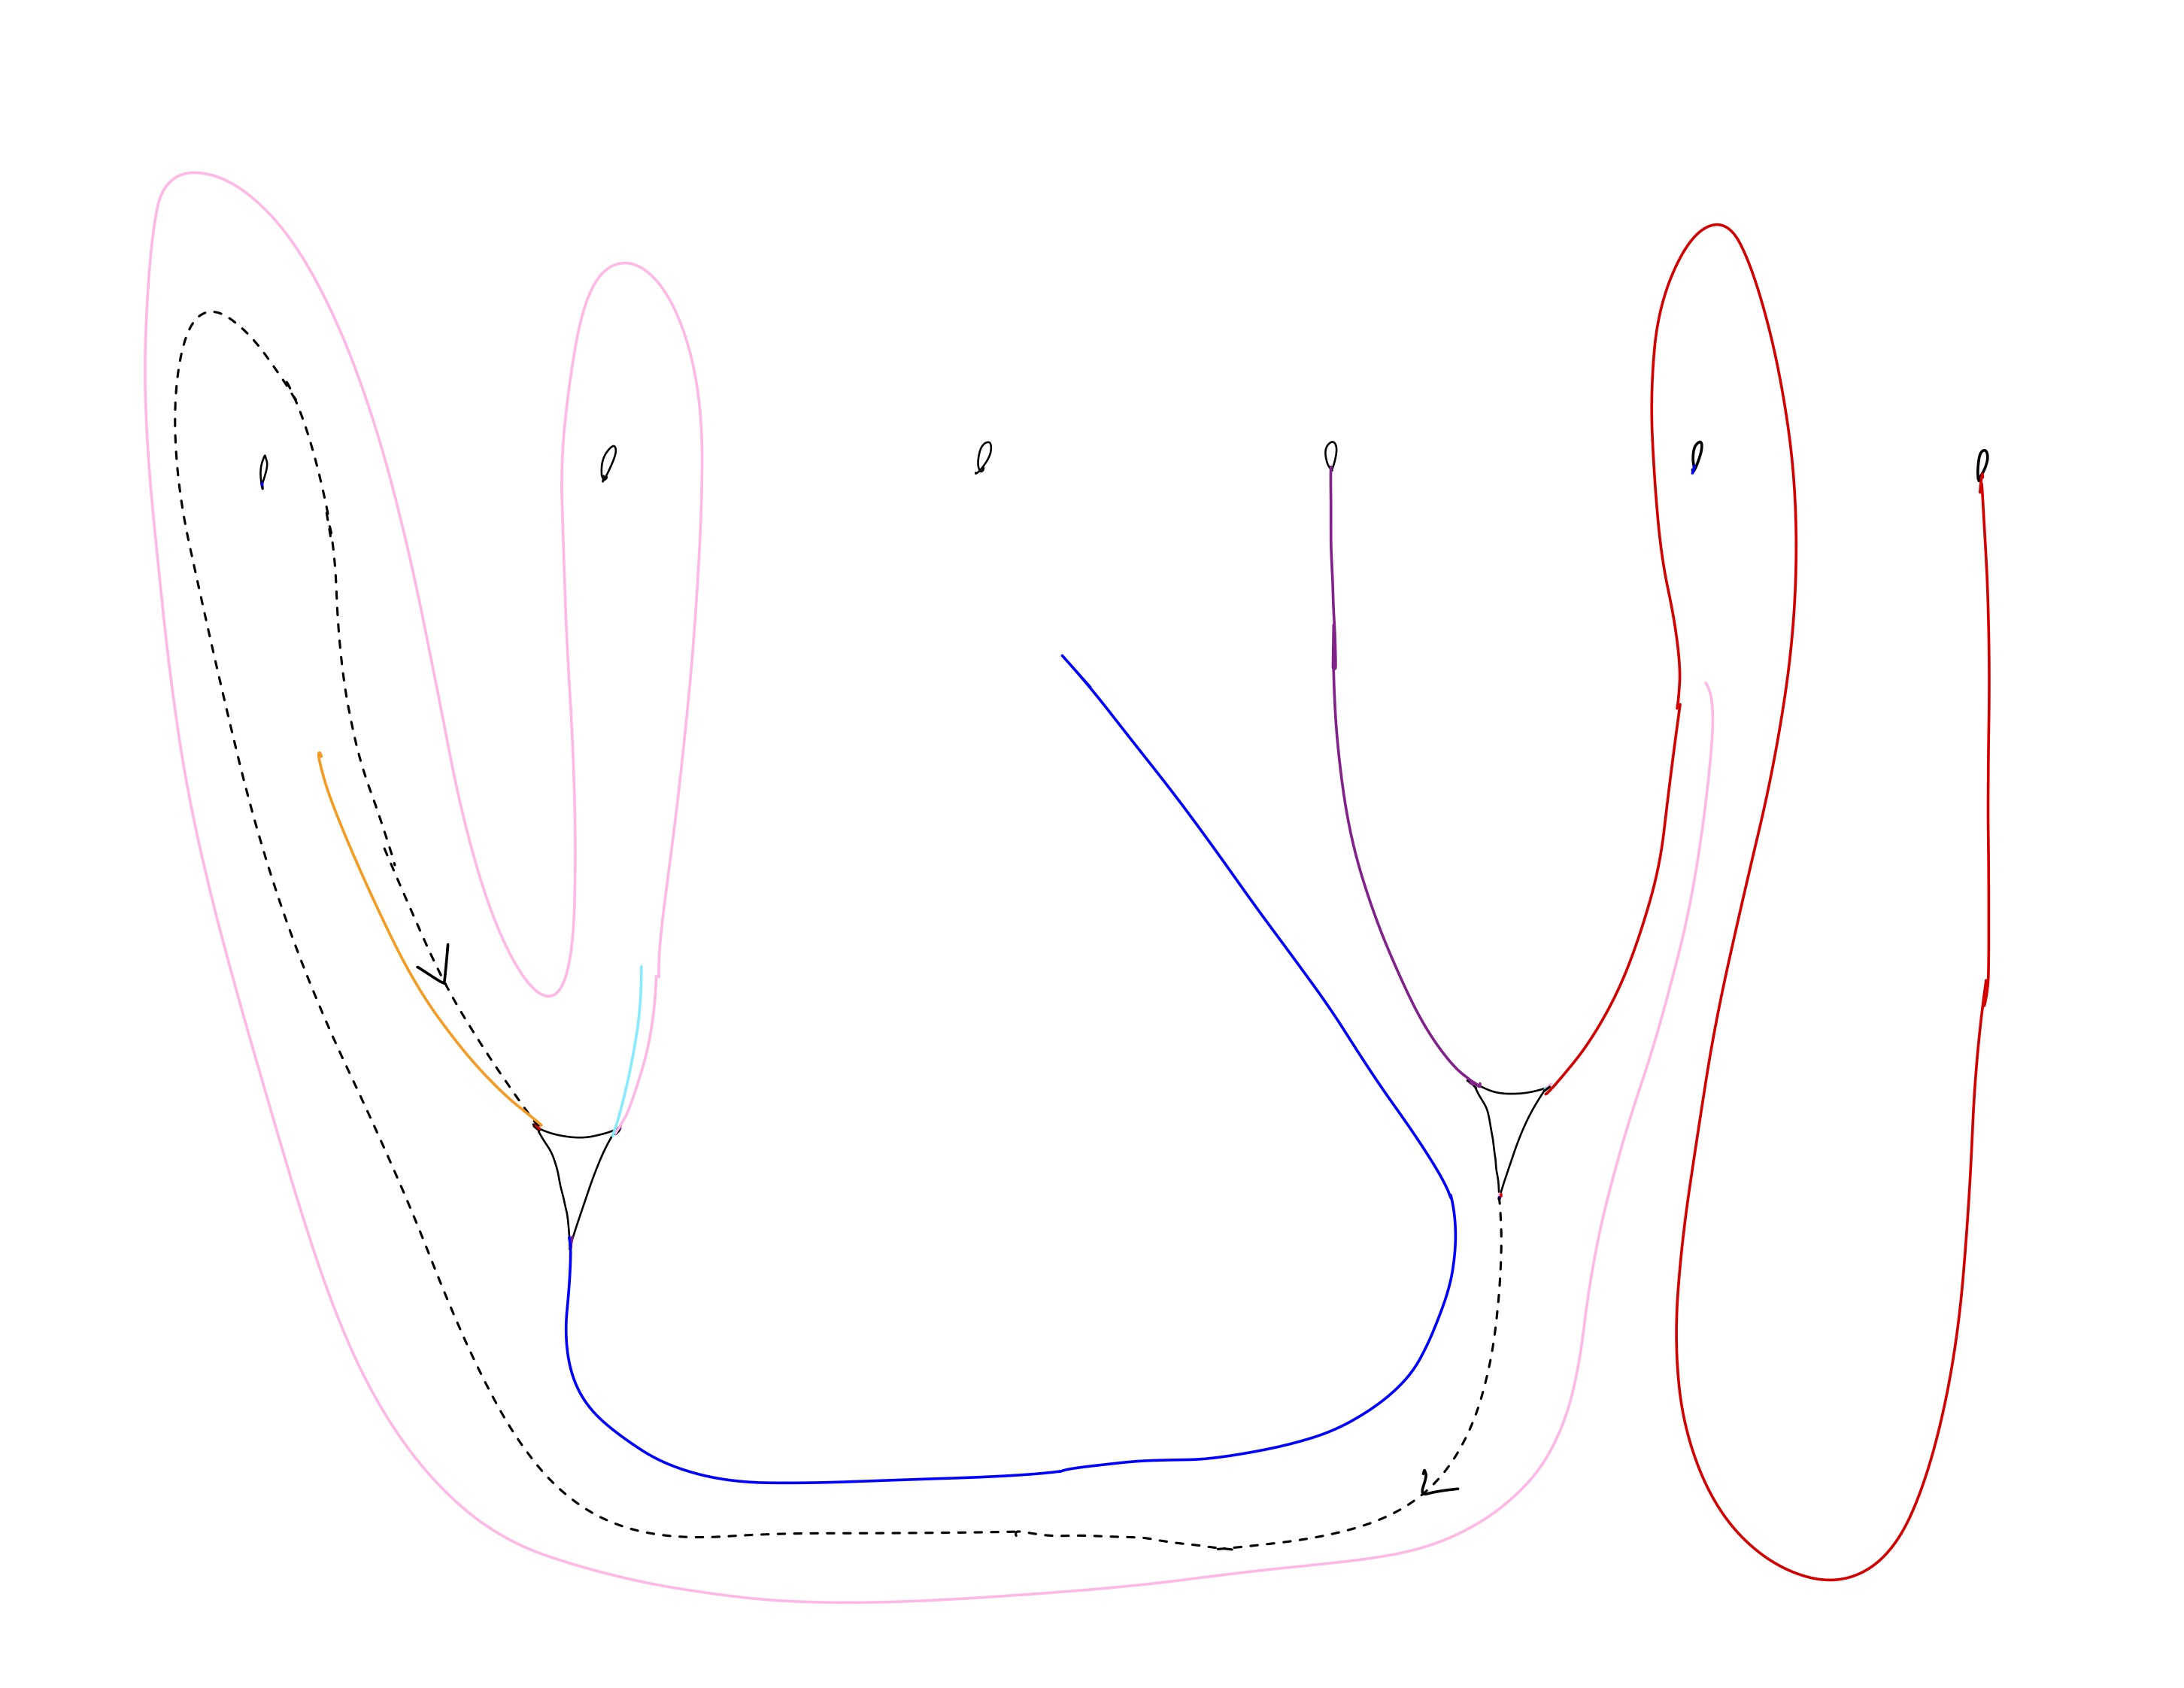
\includegraphics[width=\linewidth]{figures_case_analysis/track17_case_analysis/Boke-10.jpg}
    \caption{Boke10}
    \label{fig:Boke10}
\end{figure}

\begin{figure}[ht]
    \centering
    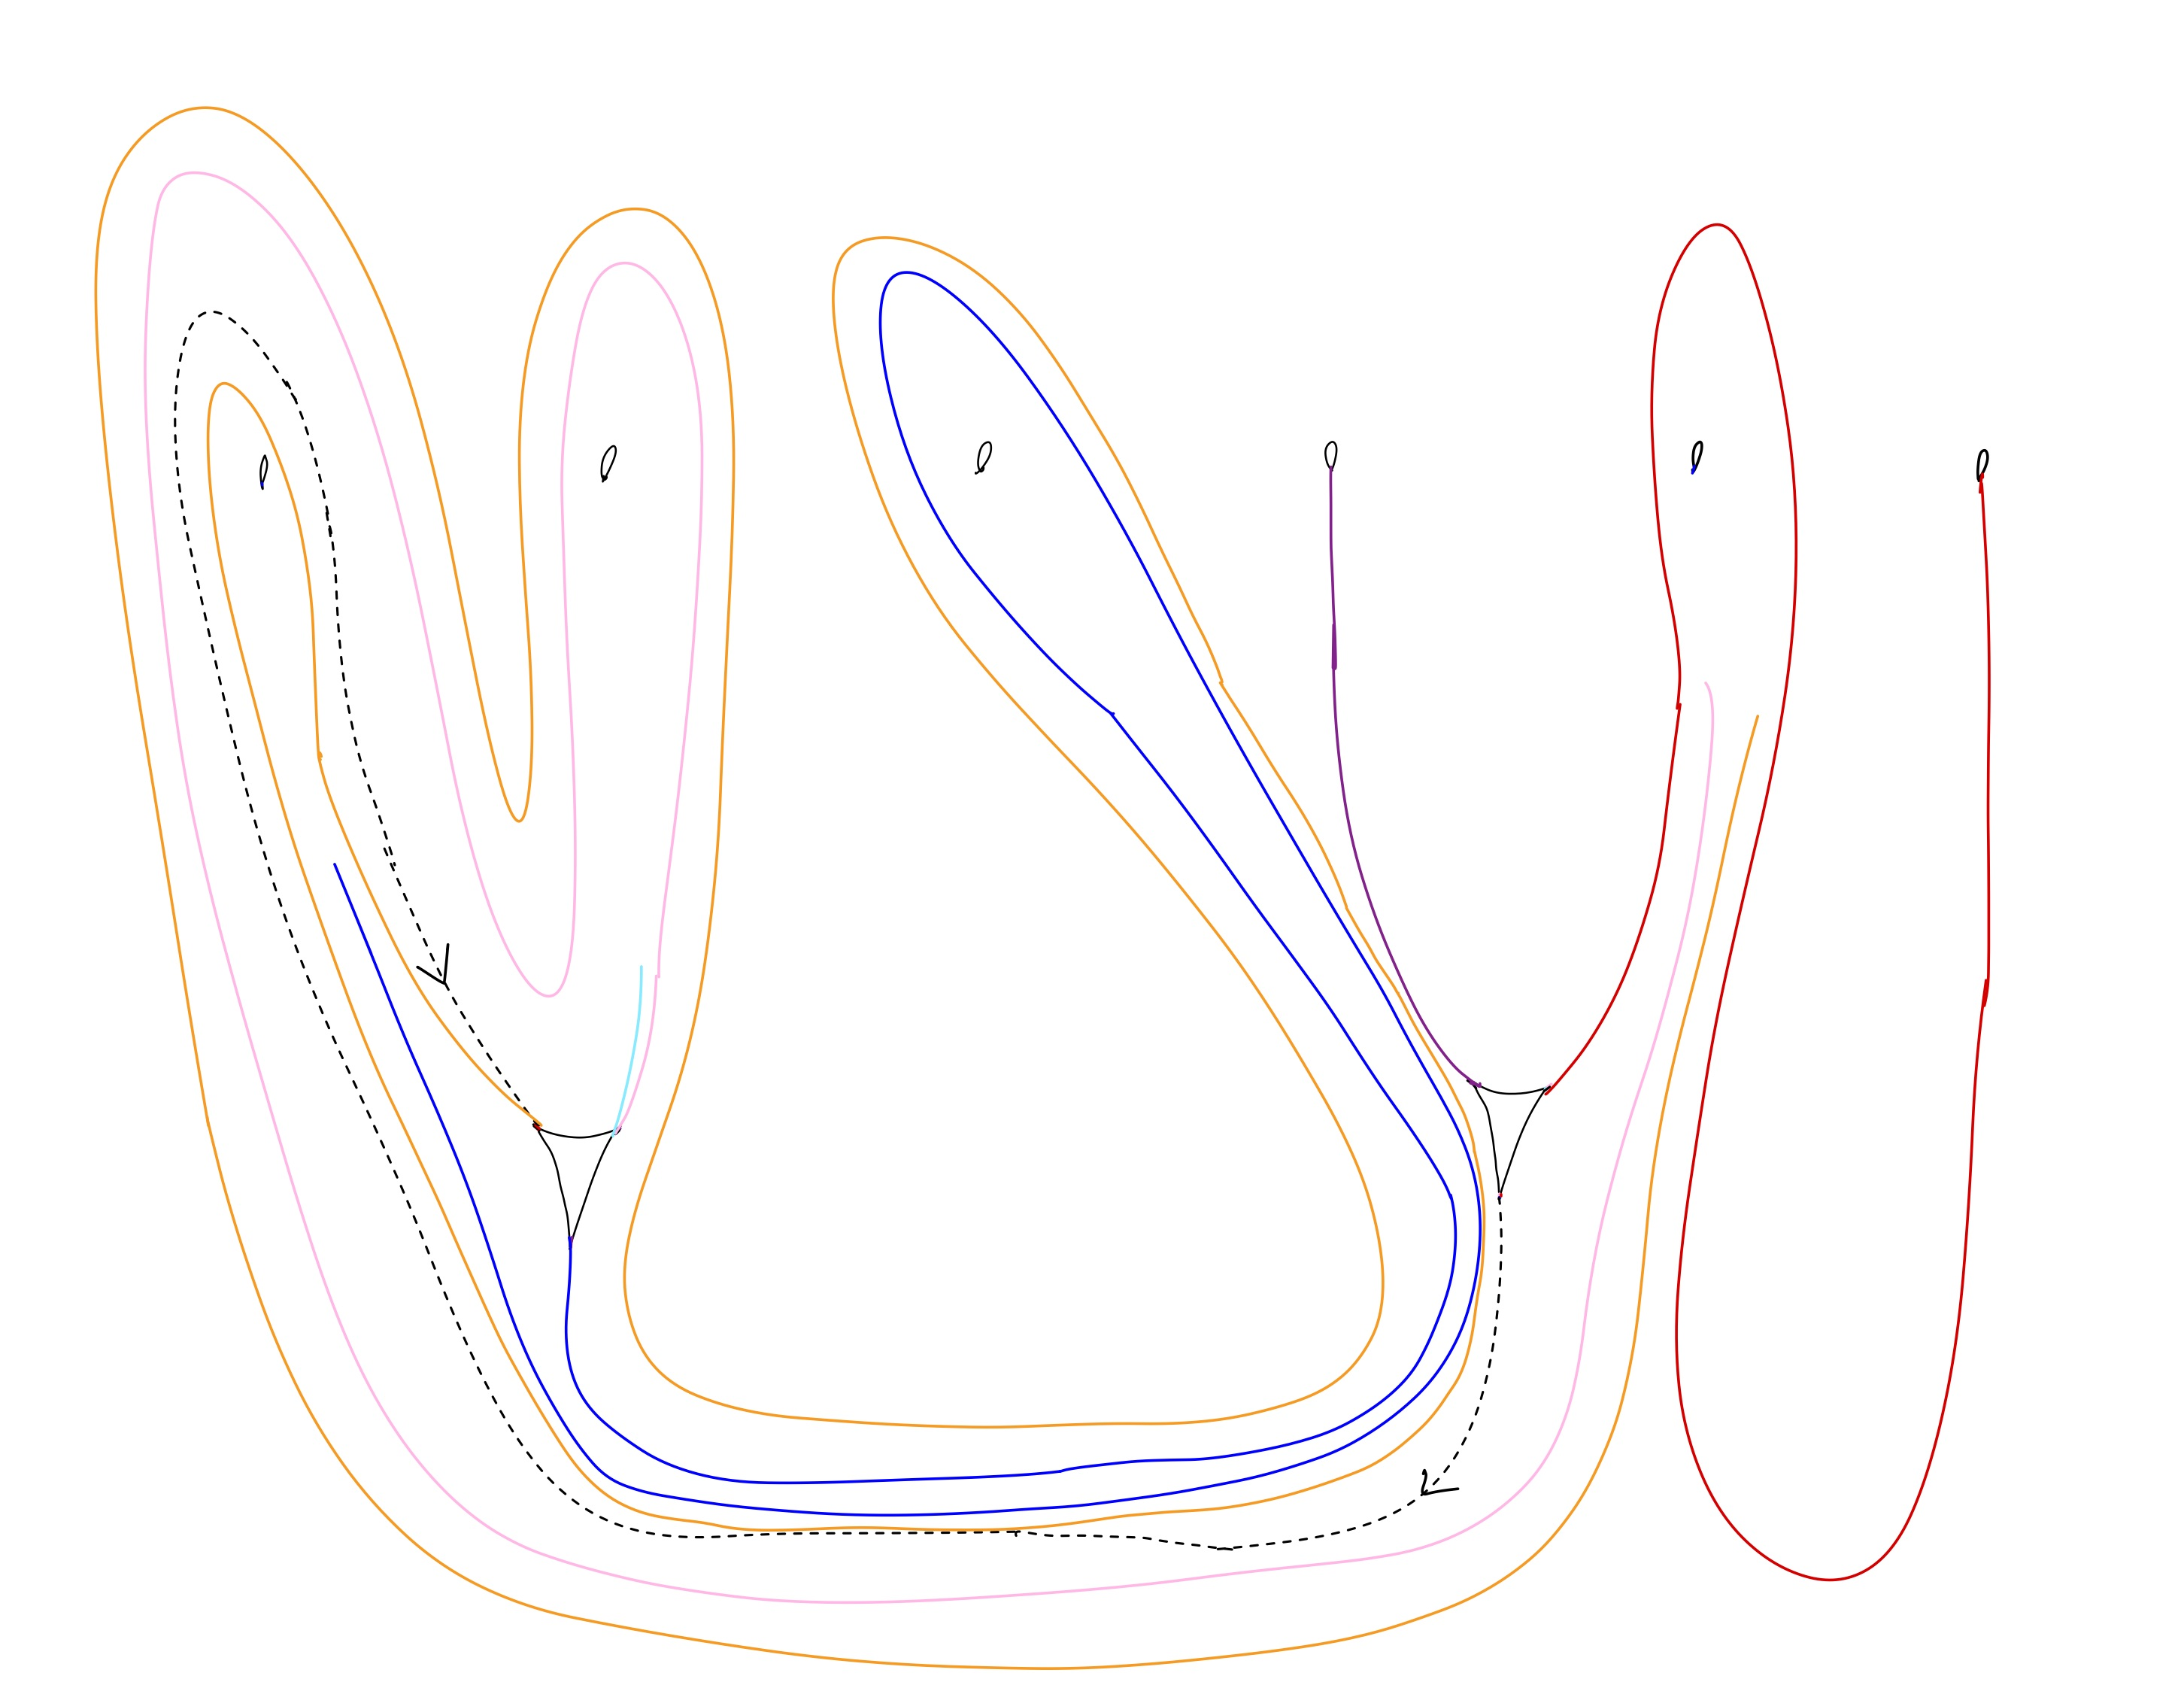
\includegraphics[width=\linewidth]{figures_case_analysis/track17_case_analysis/Boke-11.jpg}
    \caption{Boke11}
    \label{fig:Boke11}
\end{figure}

\begin{figure}[ht]
    \centering
    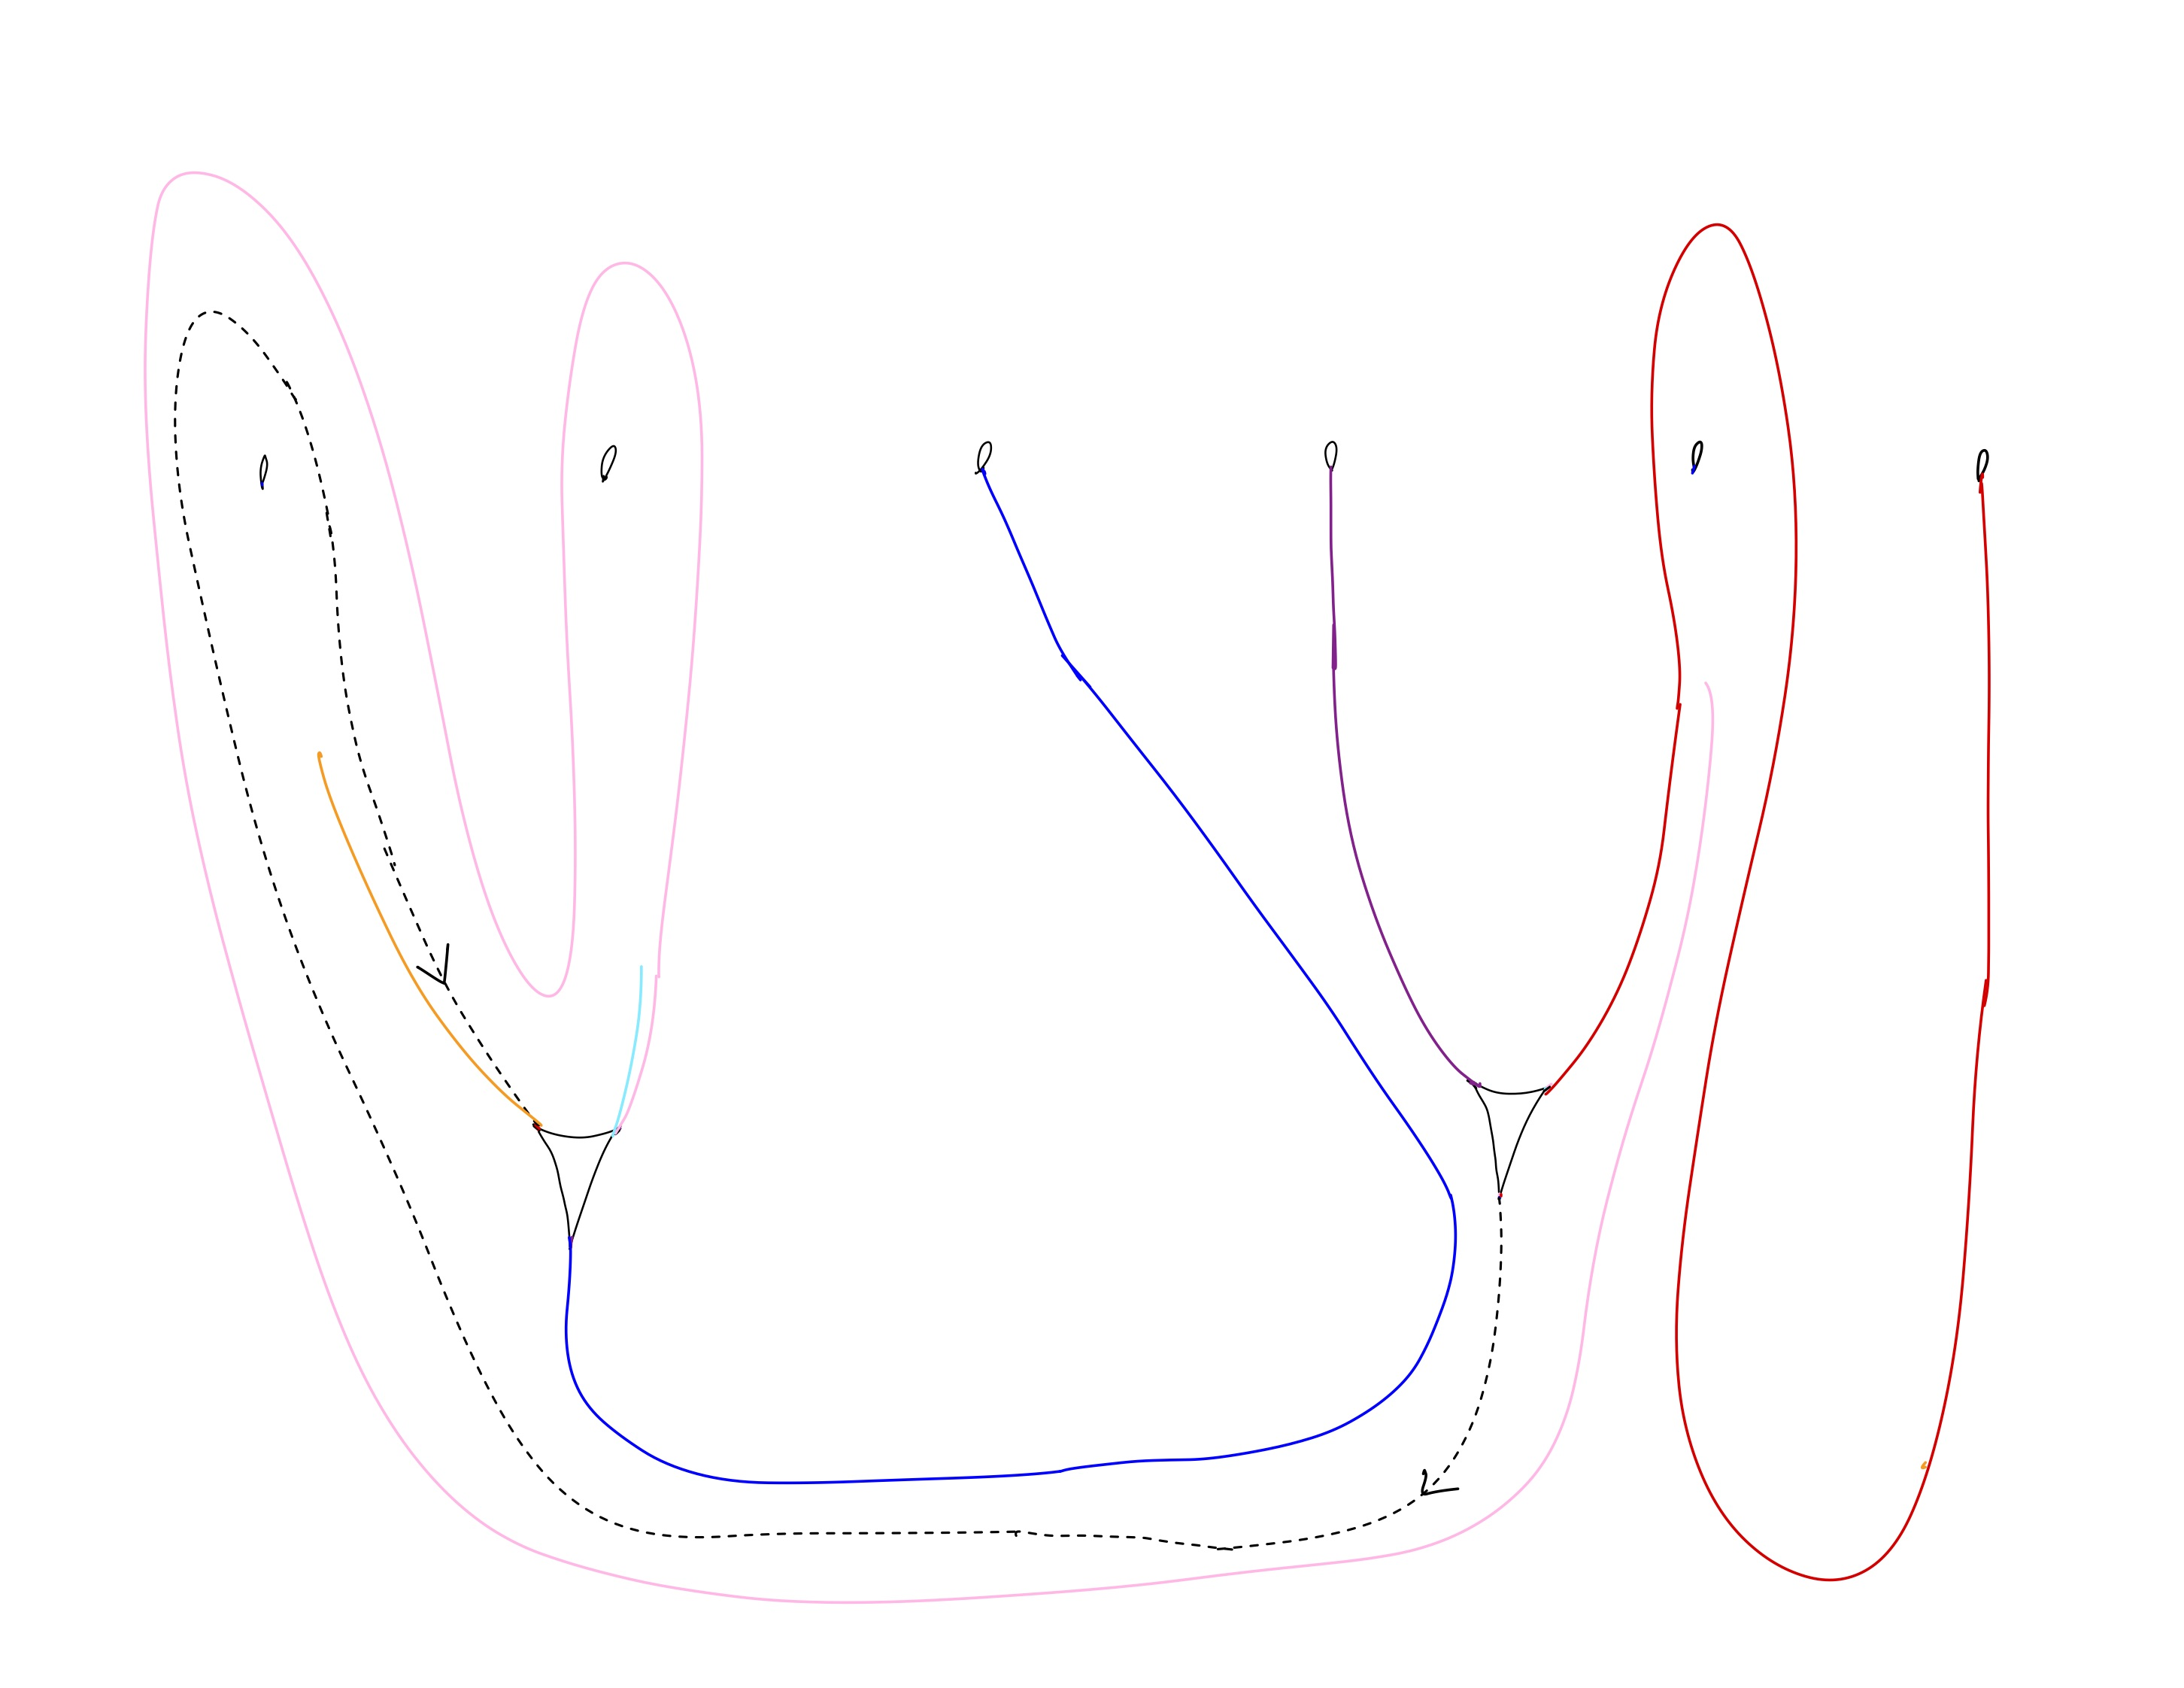
\includegraphics[width=\linewidth]{figures_case_analysis/track17_case_analysis/Boke-12.jpg}
    \caption{Boke12}
    \label{fig:Boke12}
\end{figure}

\begin{figure}[ht]
    \centering
    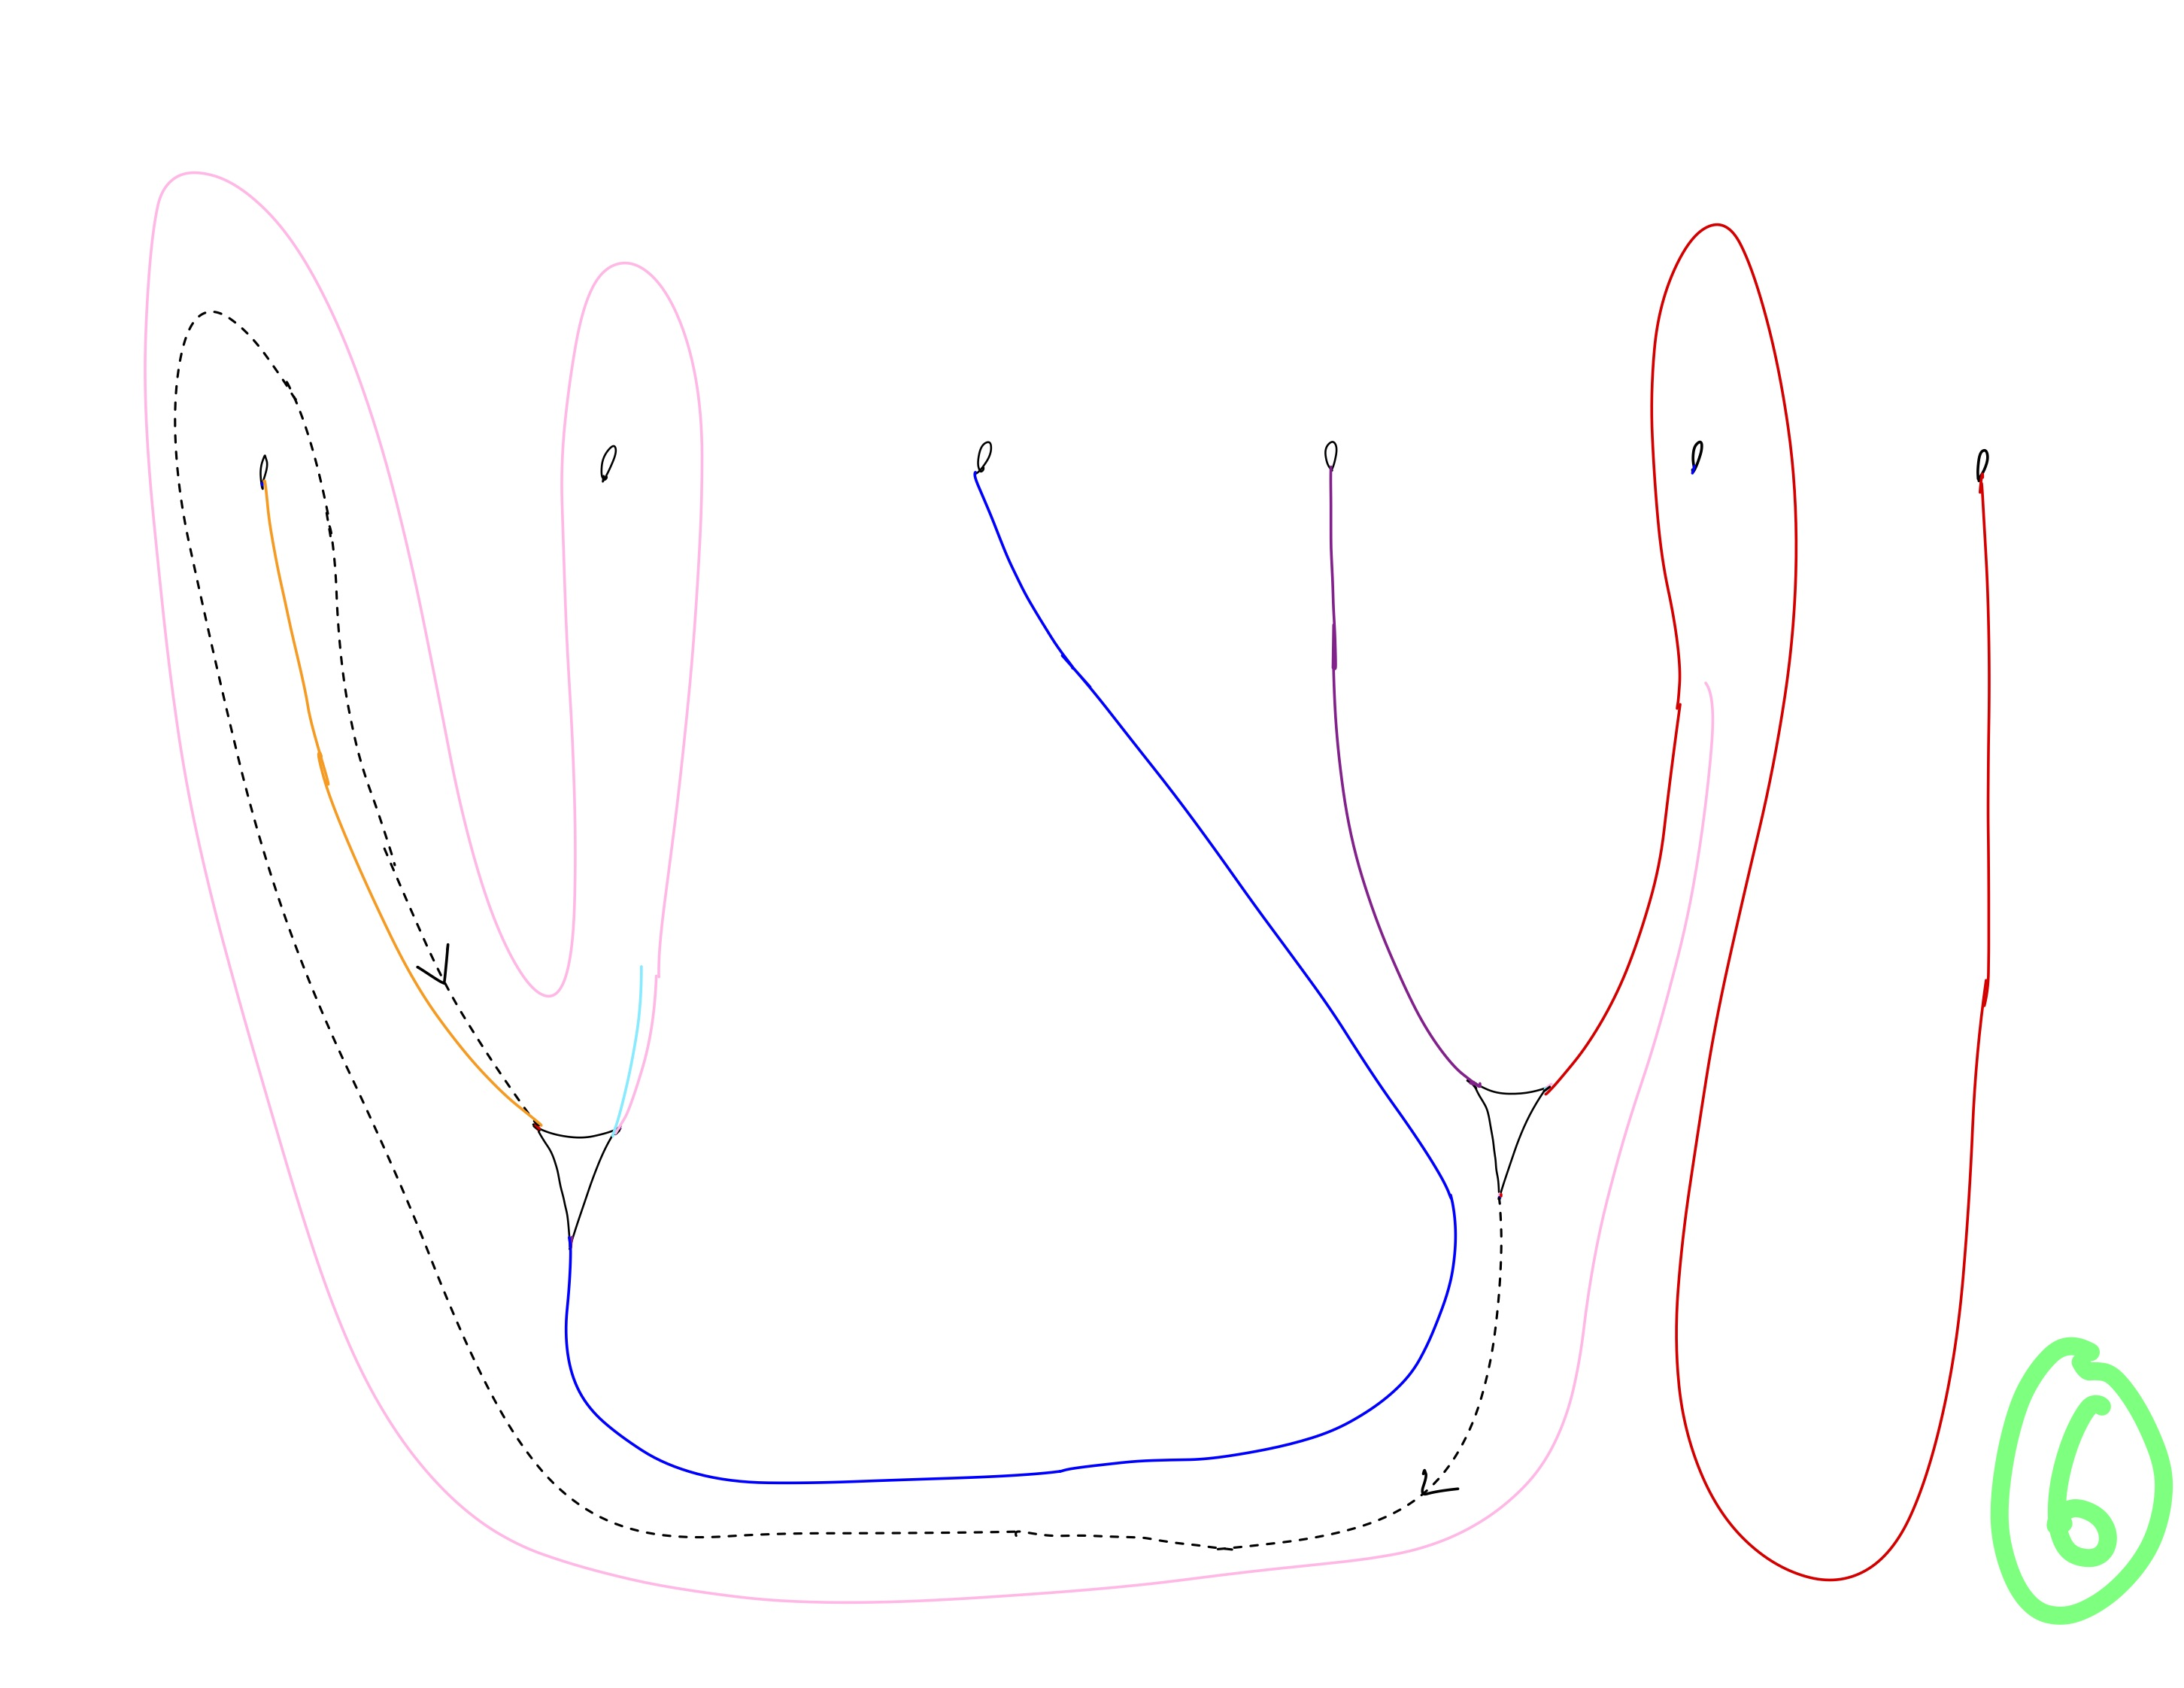
\includegraphics[width=\linewidth]{figures_case_analysis/track17_case_analysis/Boke-13.jpg}
    \caption{Boke13}
    \label{fig:Boke13}
\end{figure}
\clearpage

\begin{figure}[ht]
    \centering
    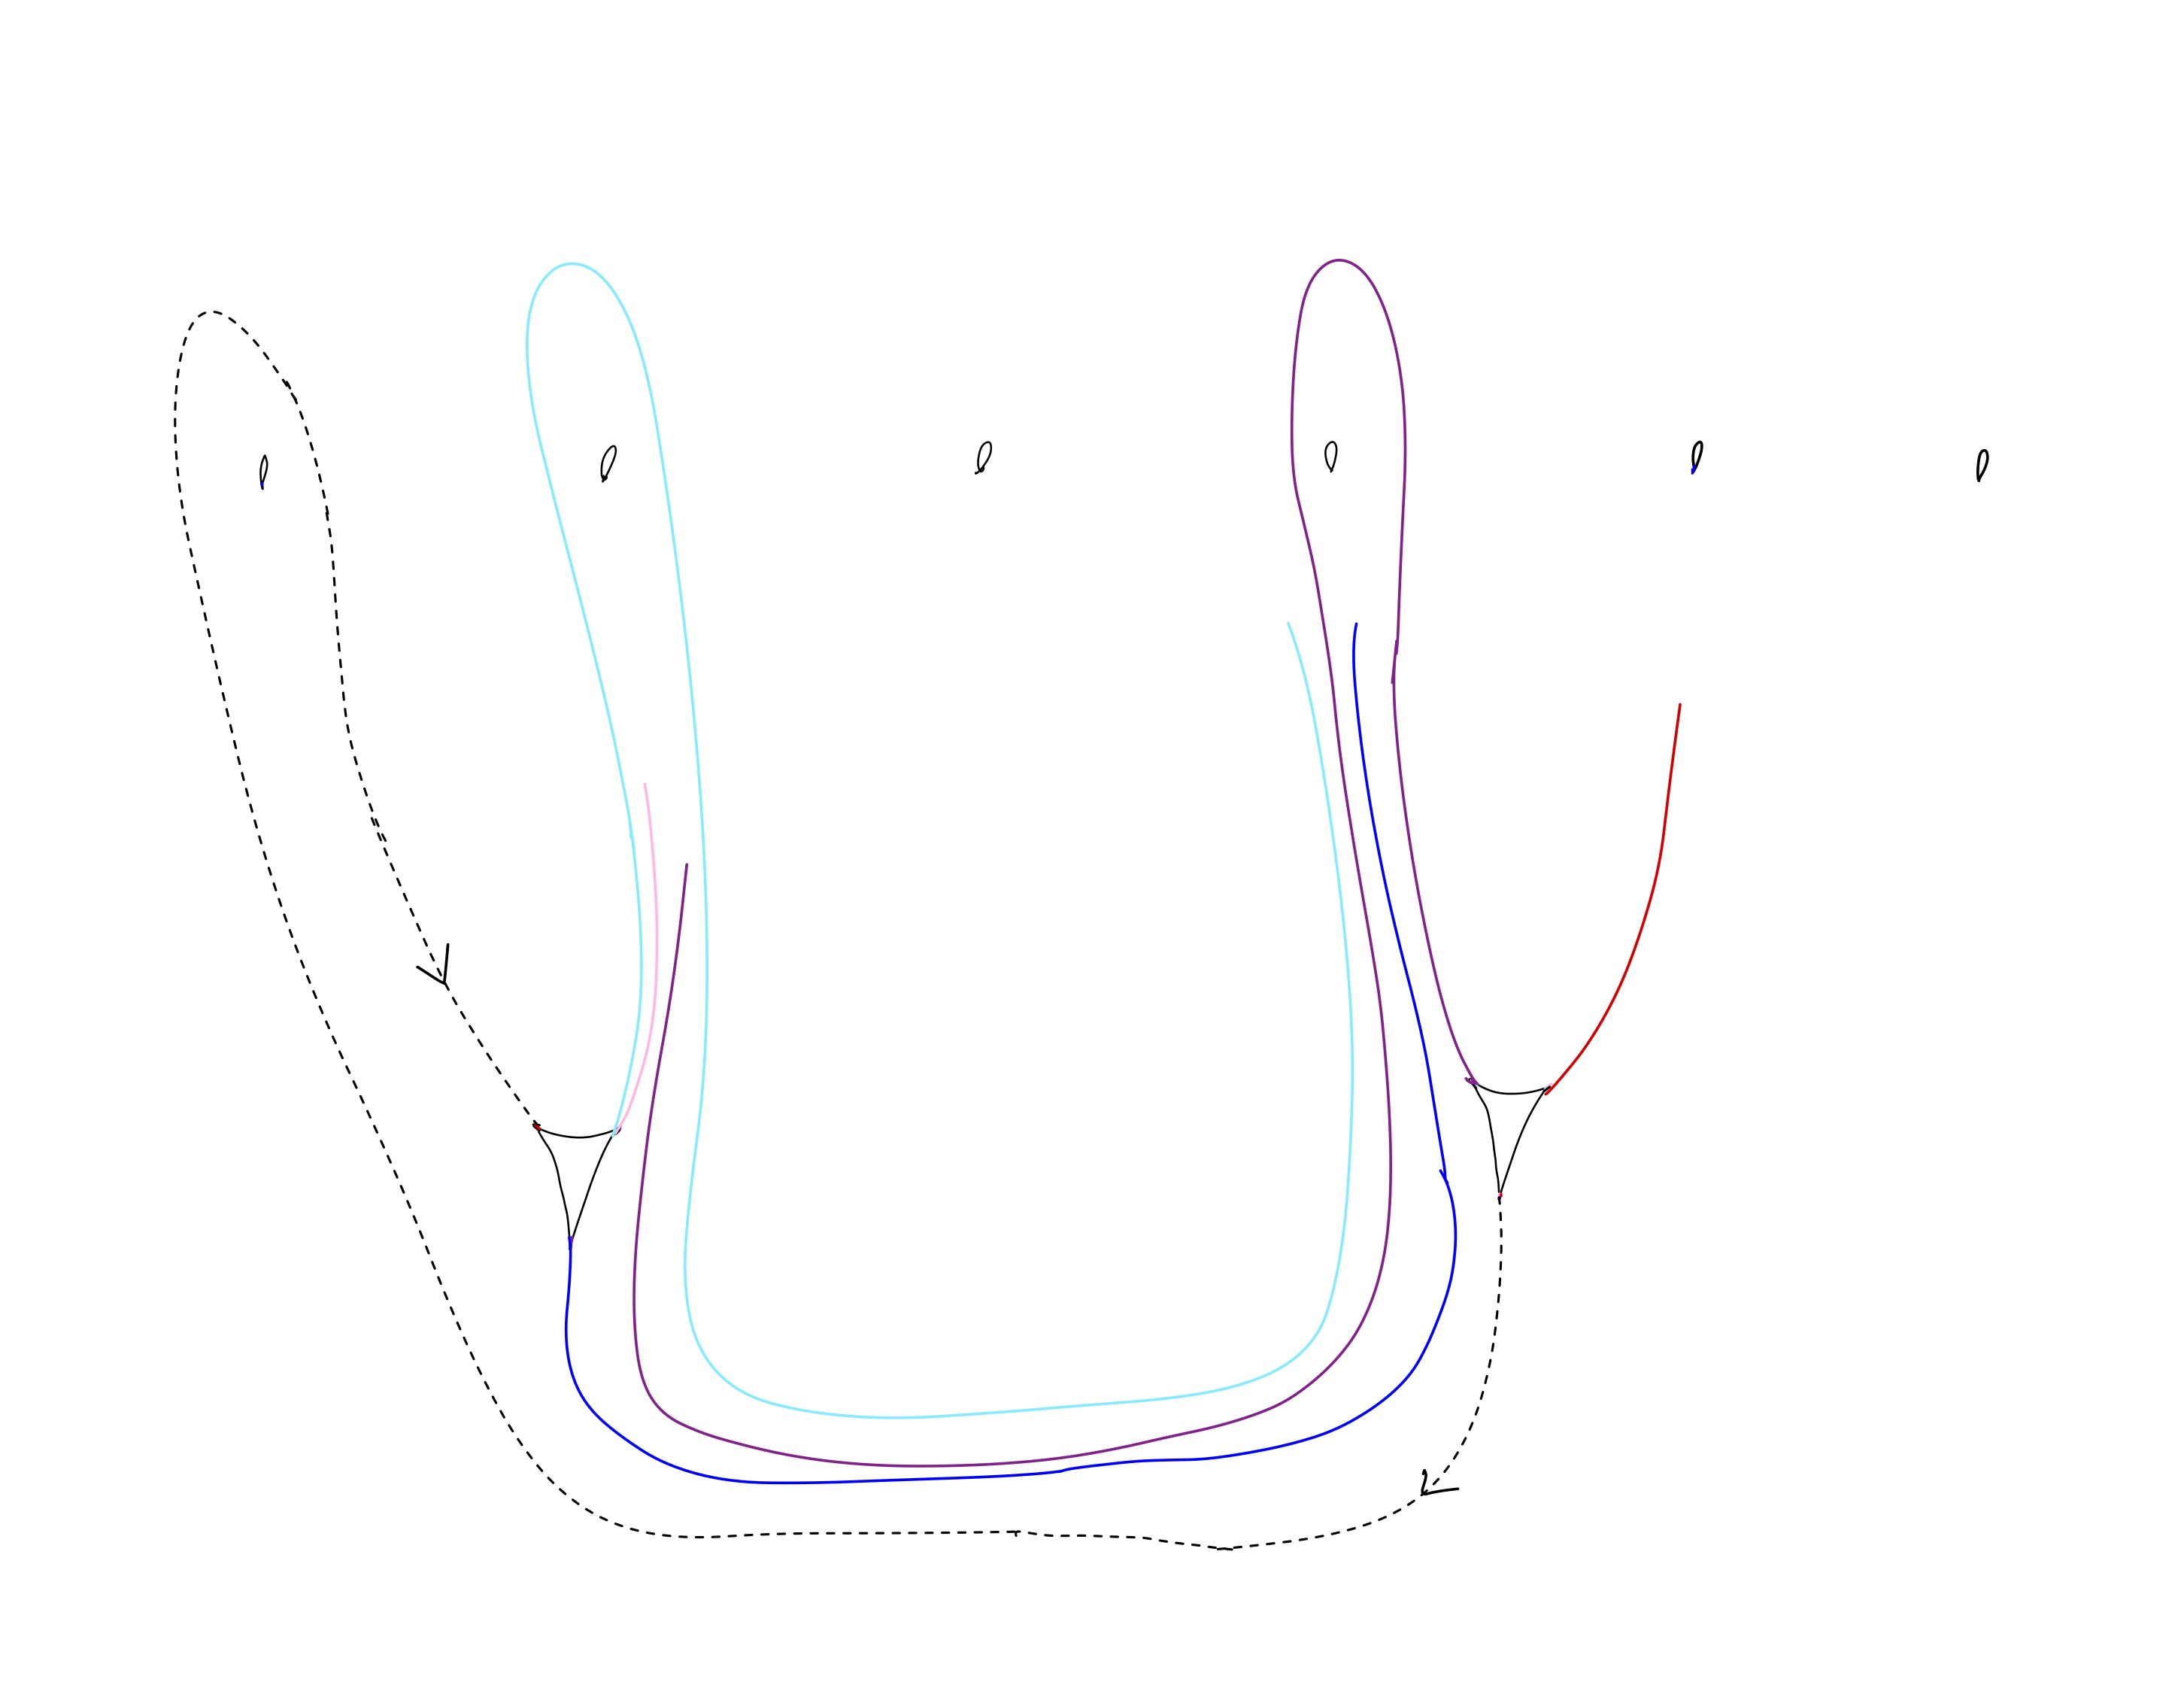
\includegraphics[width=\linewidth]{figures_case_analysis/track17_case_analysis/Clat.jpg}
    \caption{Clat1}
    \label{fig:Clat1}
\end{figure}
\clearpage

\begin{figure}[ht]
    \centering
    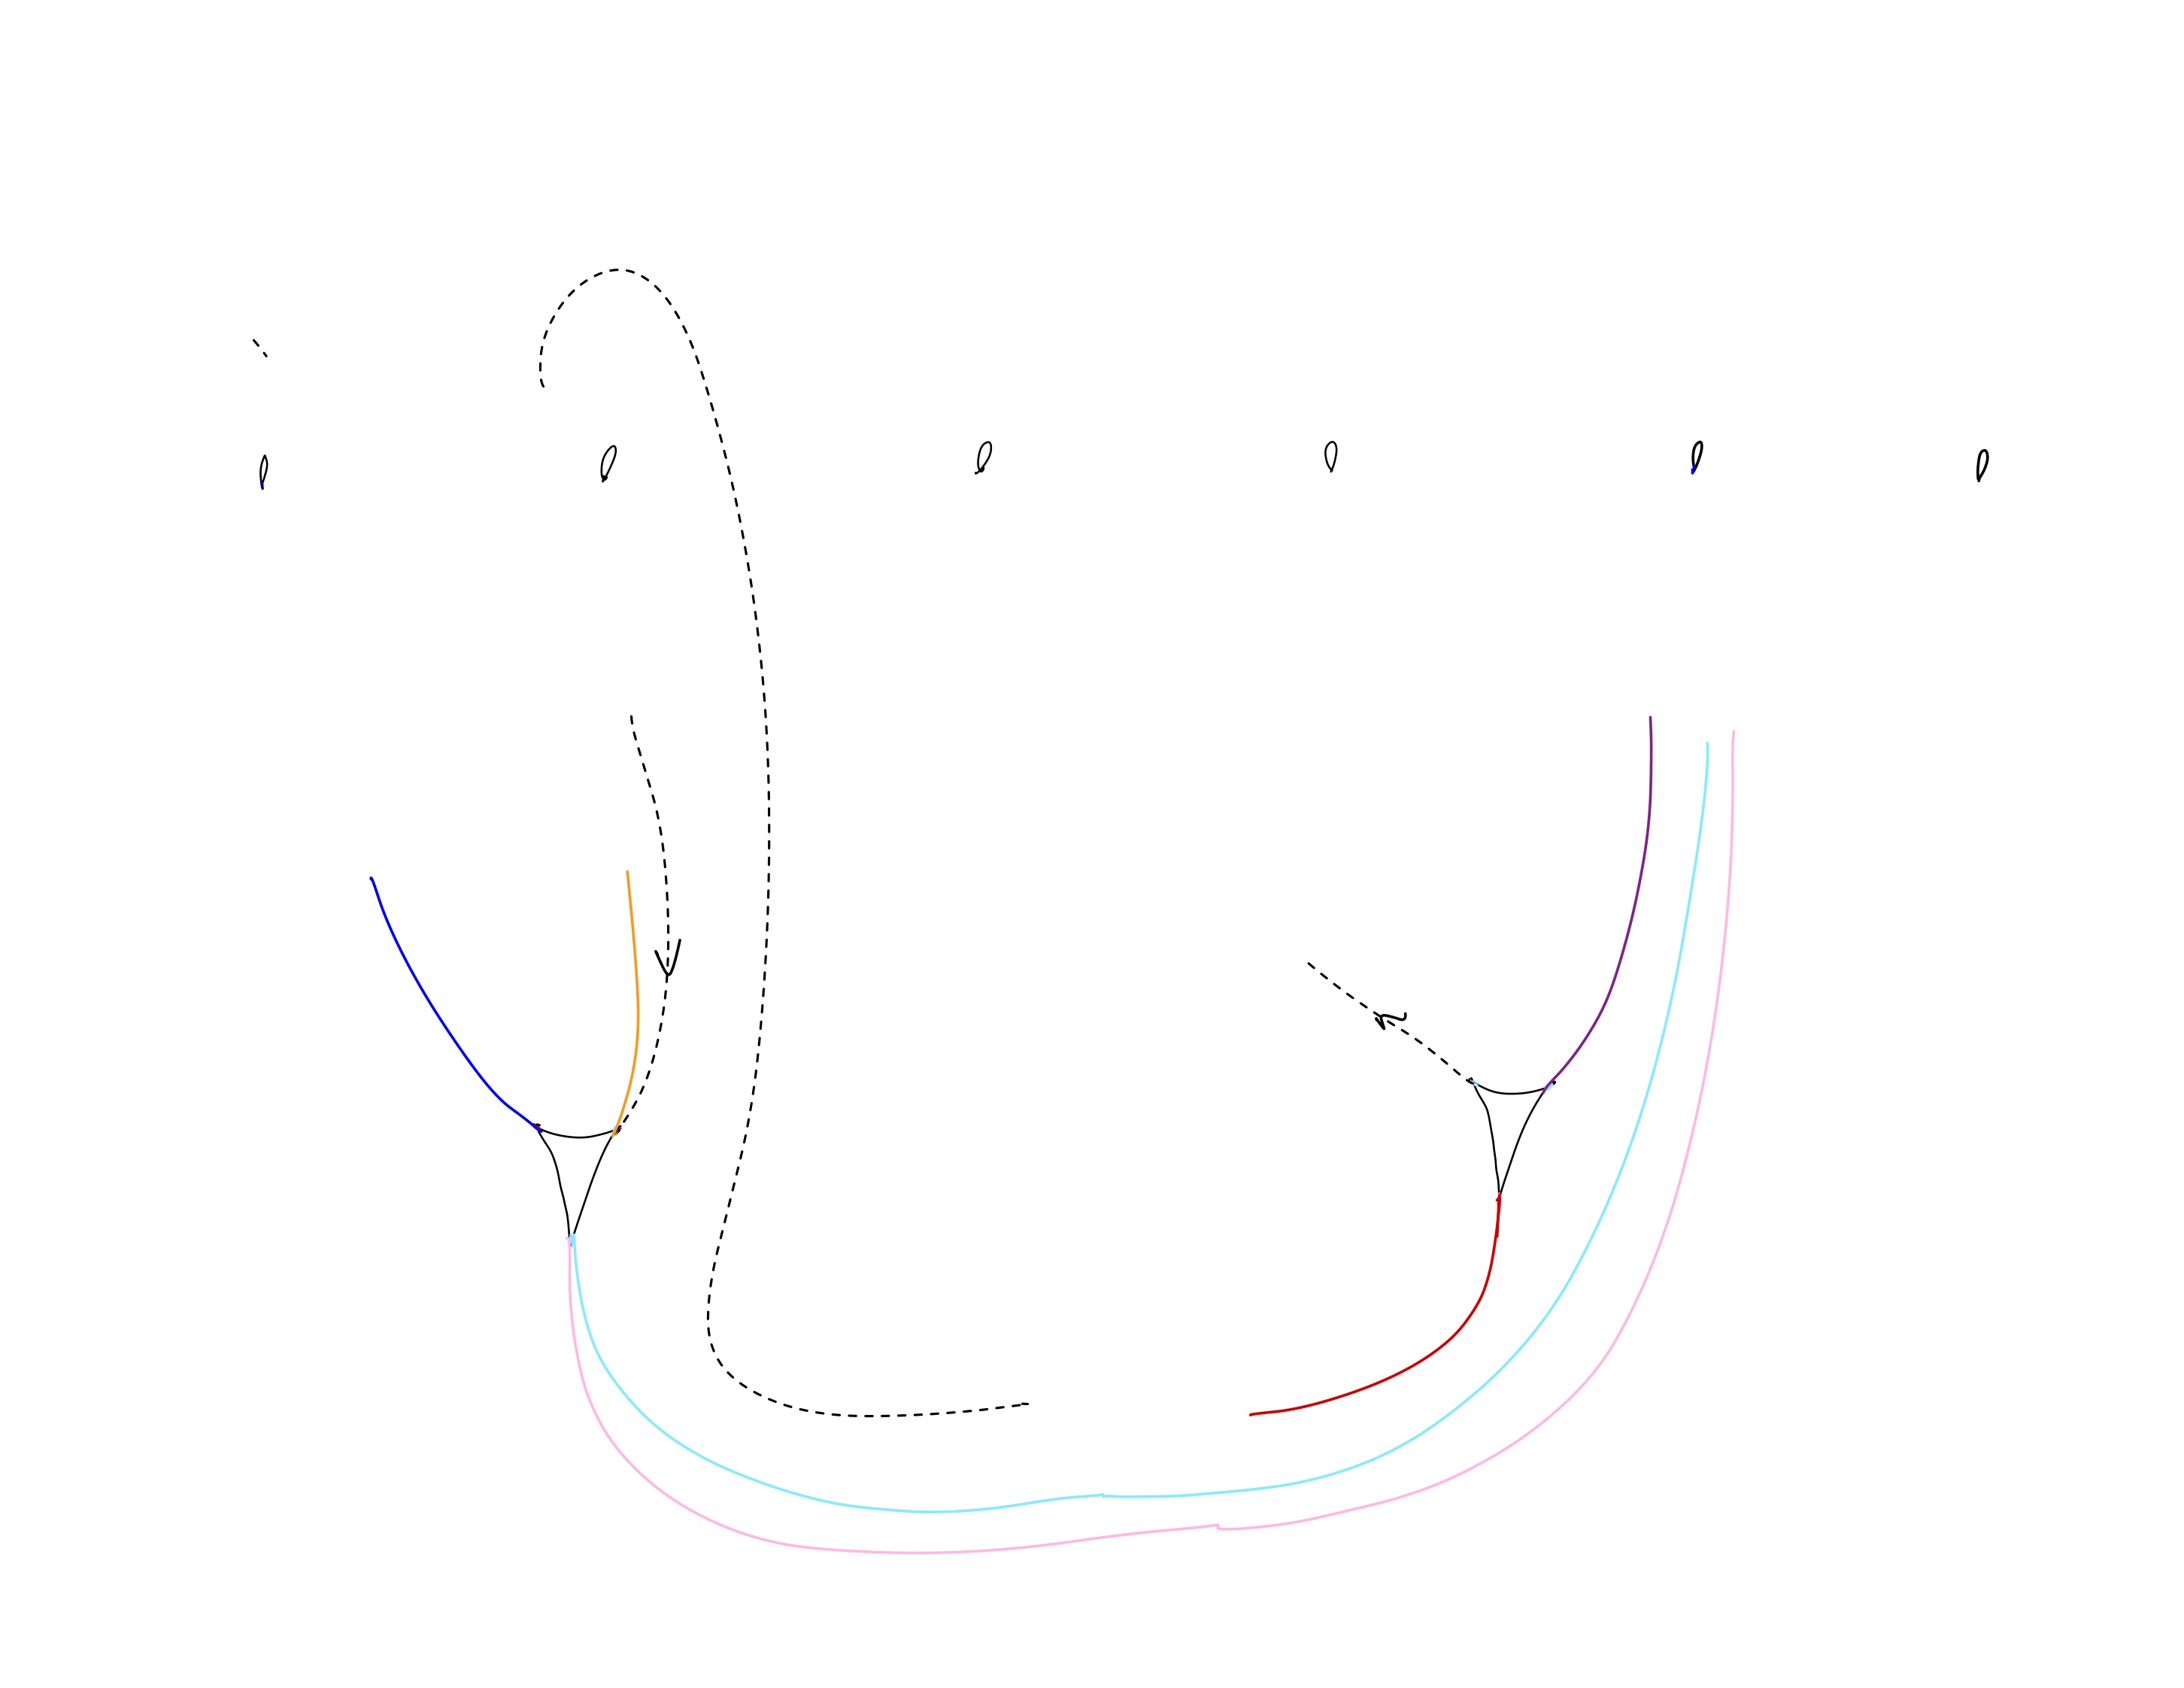
\includegraphics[width=\linewidth]{figures_case_analysis/track17_case_analysis/MMU-01.jpg}
    \caption{MMU1}
    \label{fig:MMU1}
\end{figure}

\begin{figure}[ht]
    \centering
    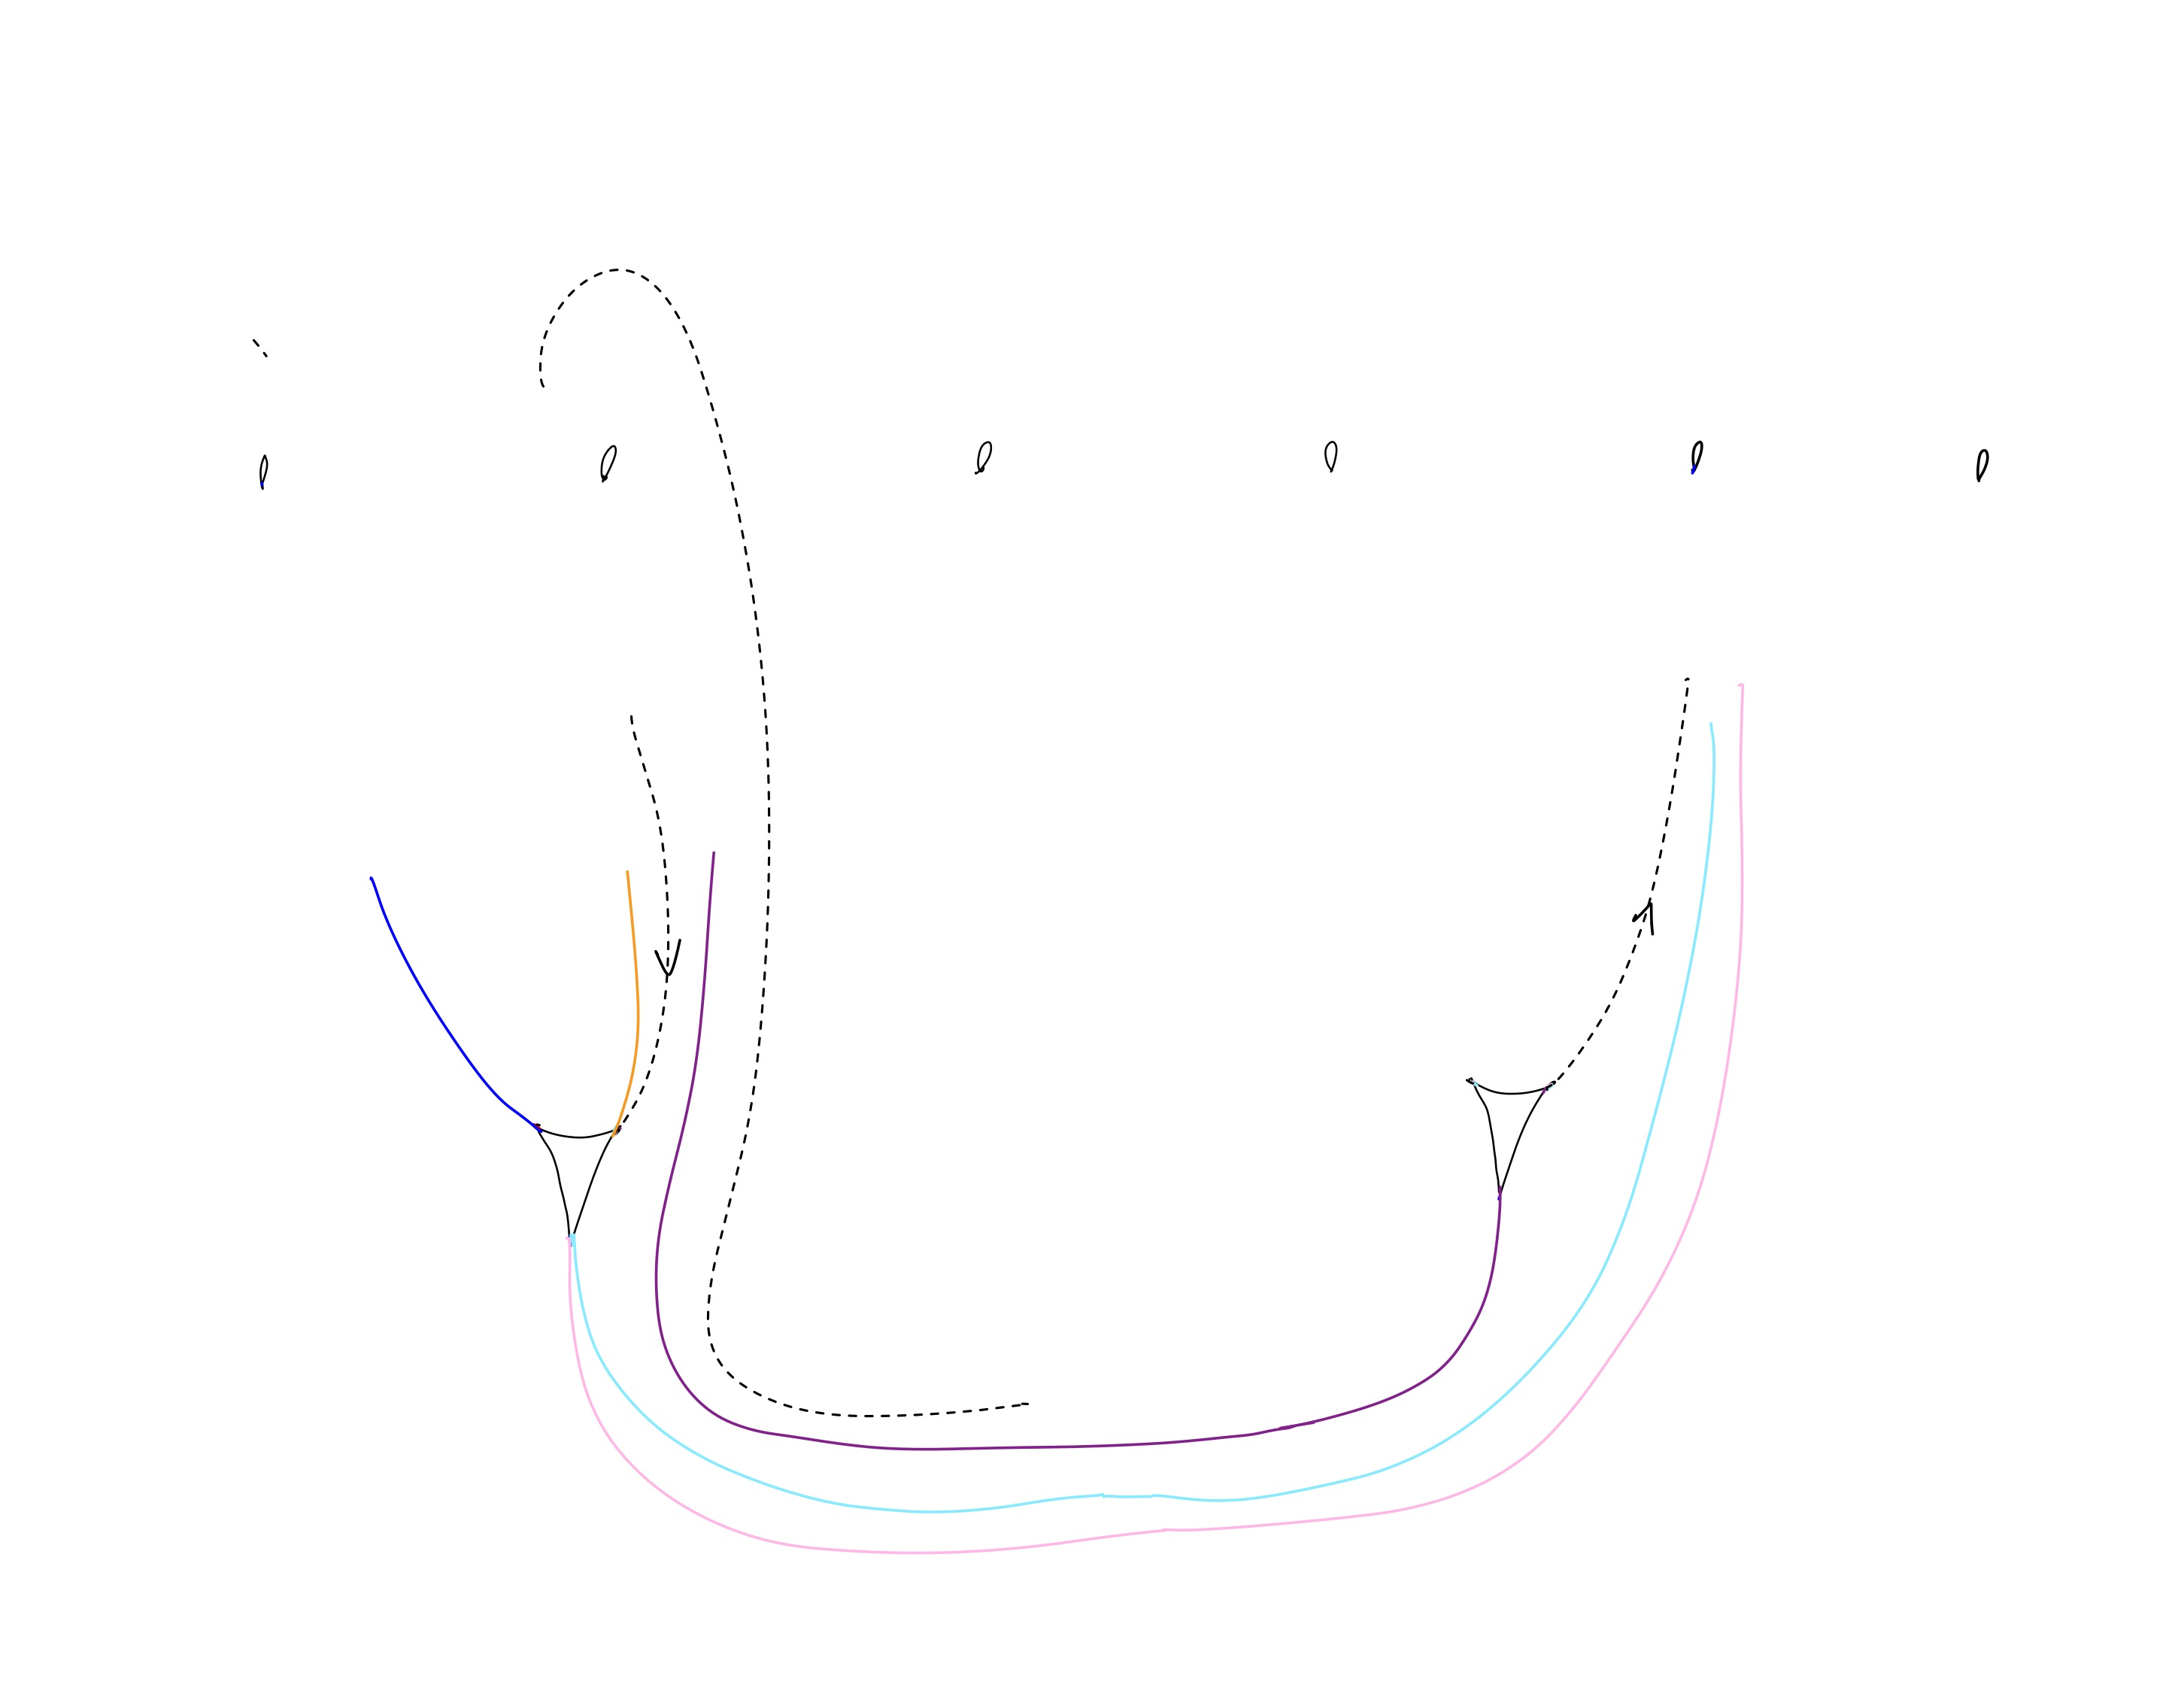
\includegraphics[width=\linewidth]{figures_case_analysis/track17_case_analysis/MMU-02.jpg}
    \caption{MMU2}
    \label{fig:MMU2}
\end{figure}

\begin{figure}[ht]
    \centering
    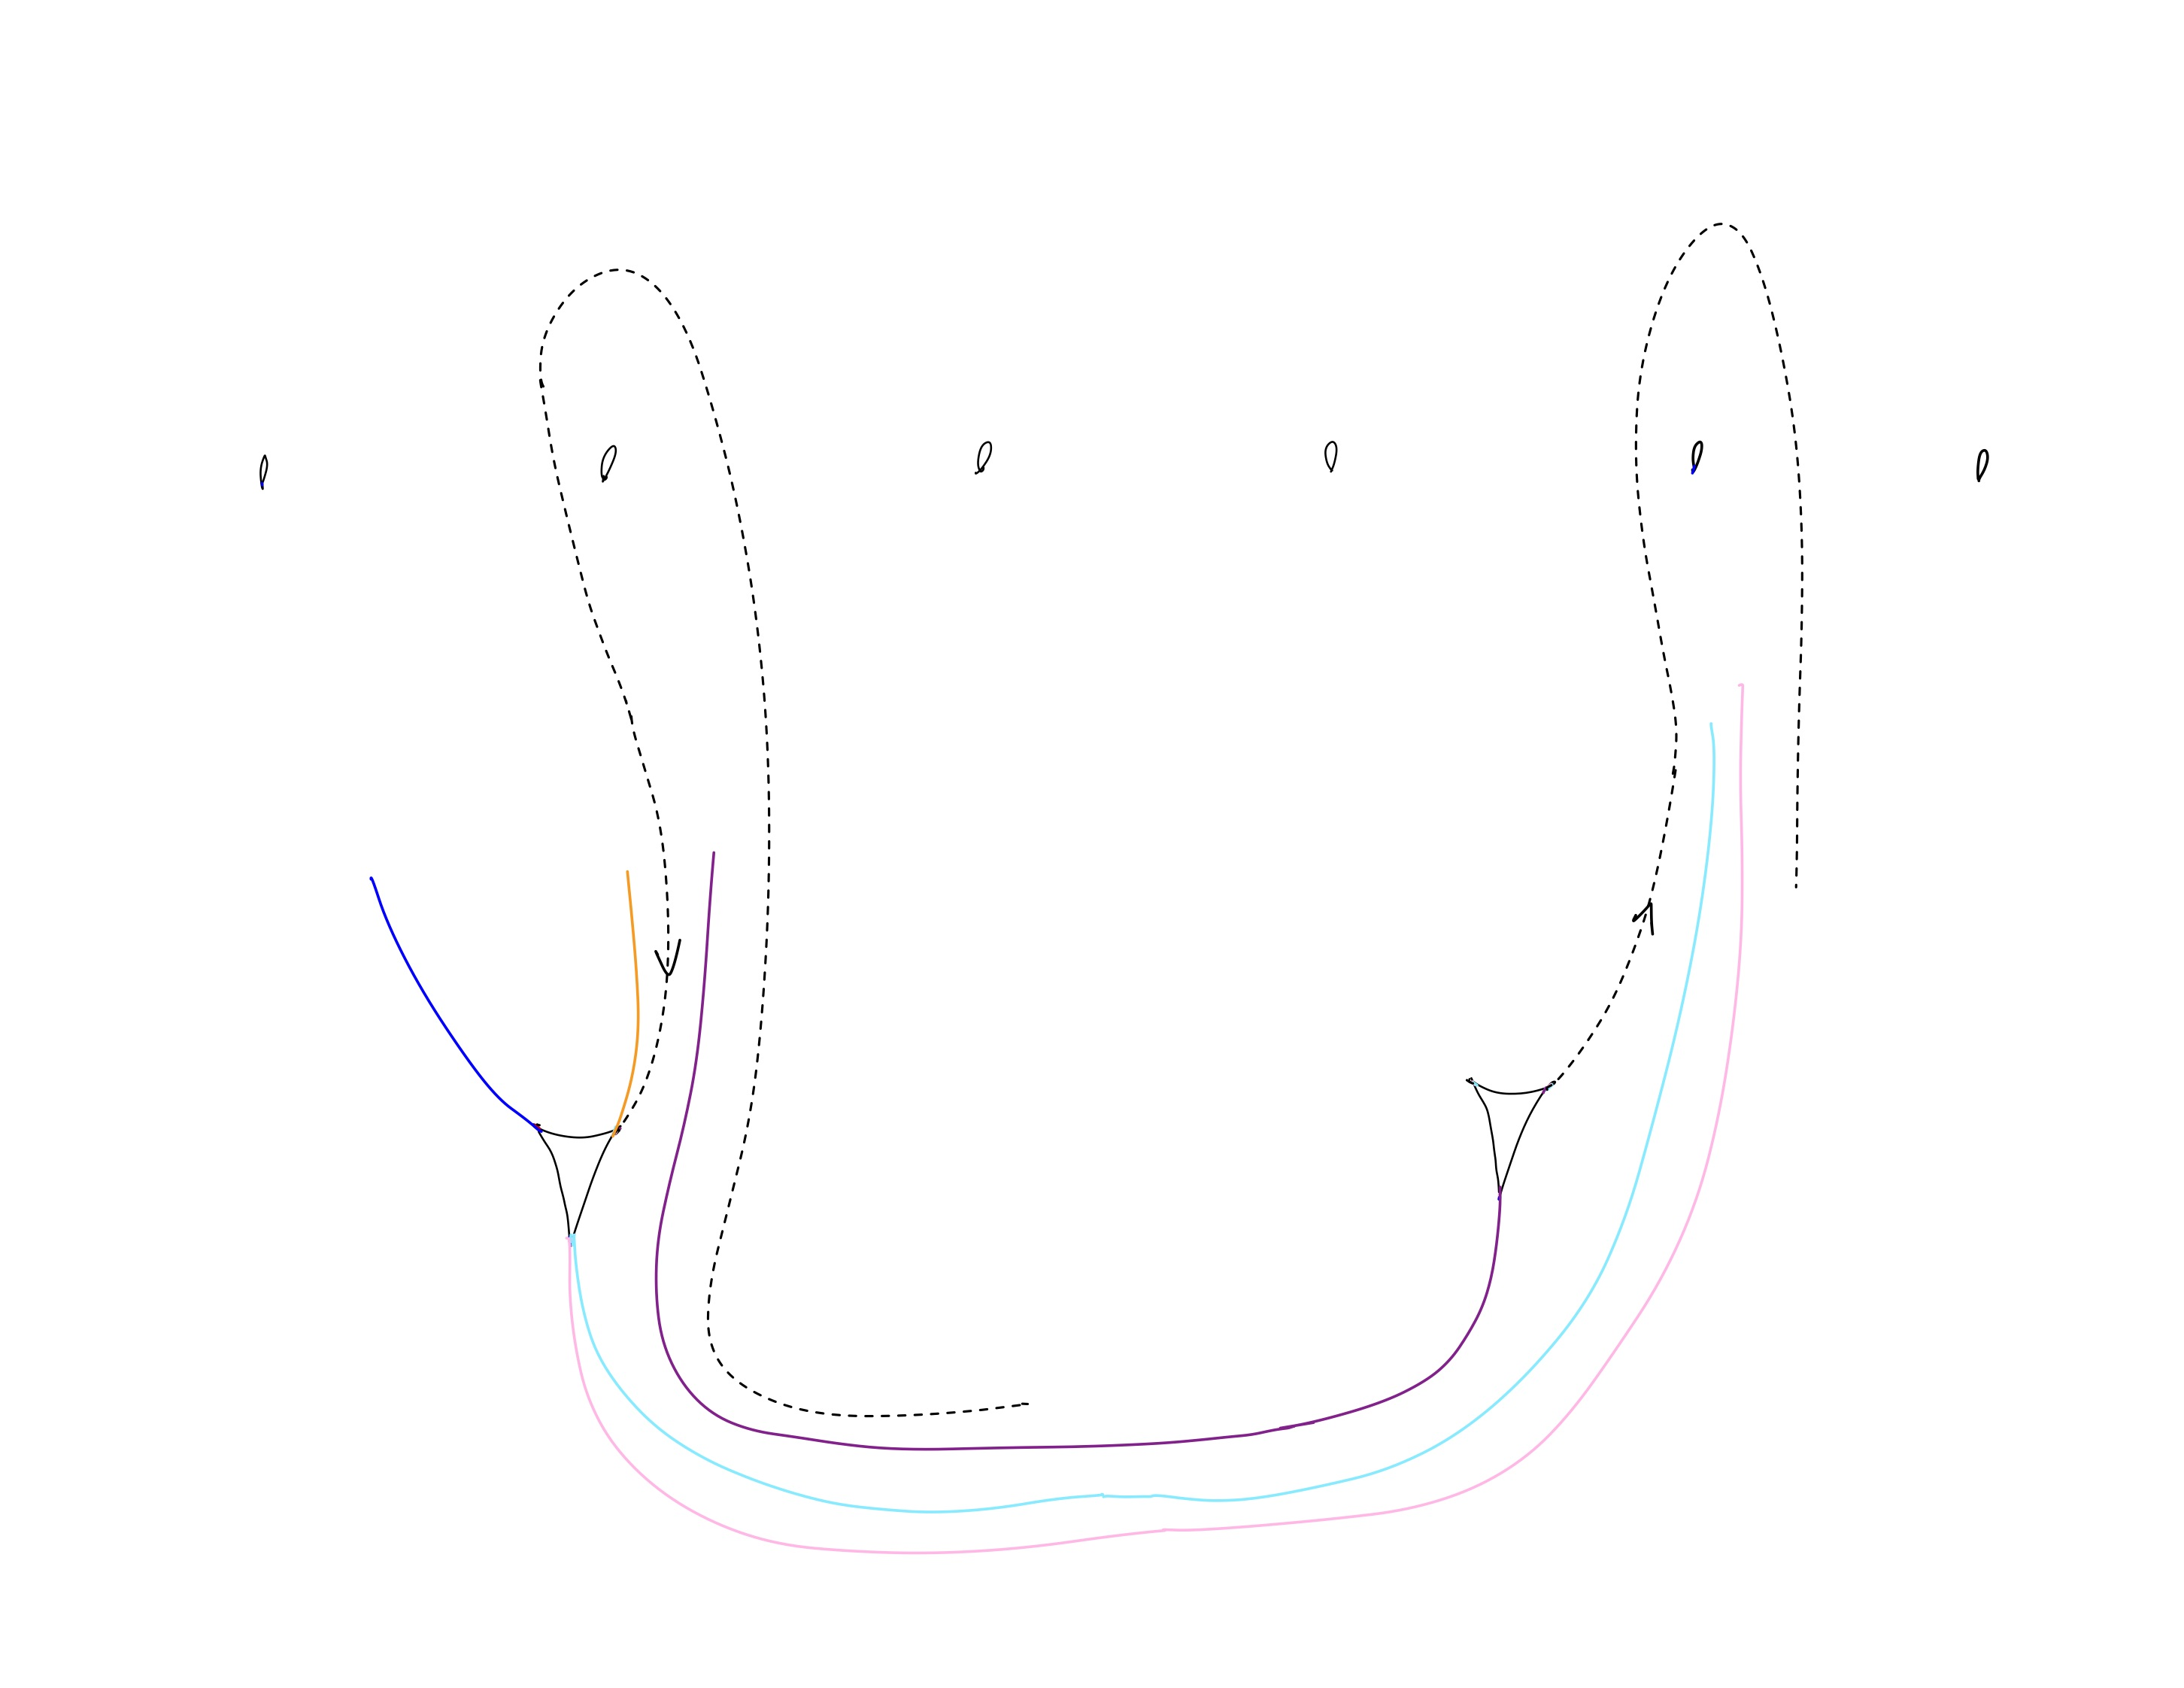
\includegraphics[width=\linewidth]{figures_case_analysis/track17_case_analysis/MMU-03.jpg}
    \caption{MMU3}
    \label{fig:MMU3}
\end{figure}

\begin{figure}[ht]
    \centering
    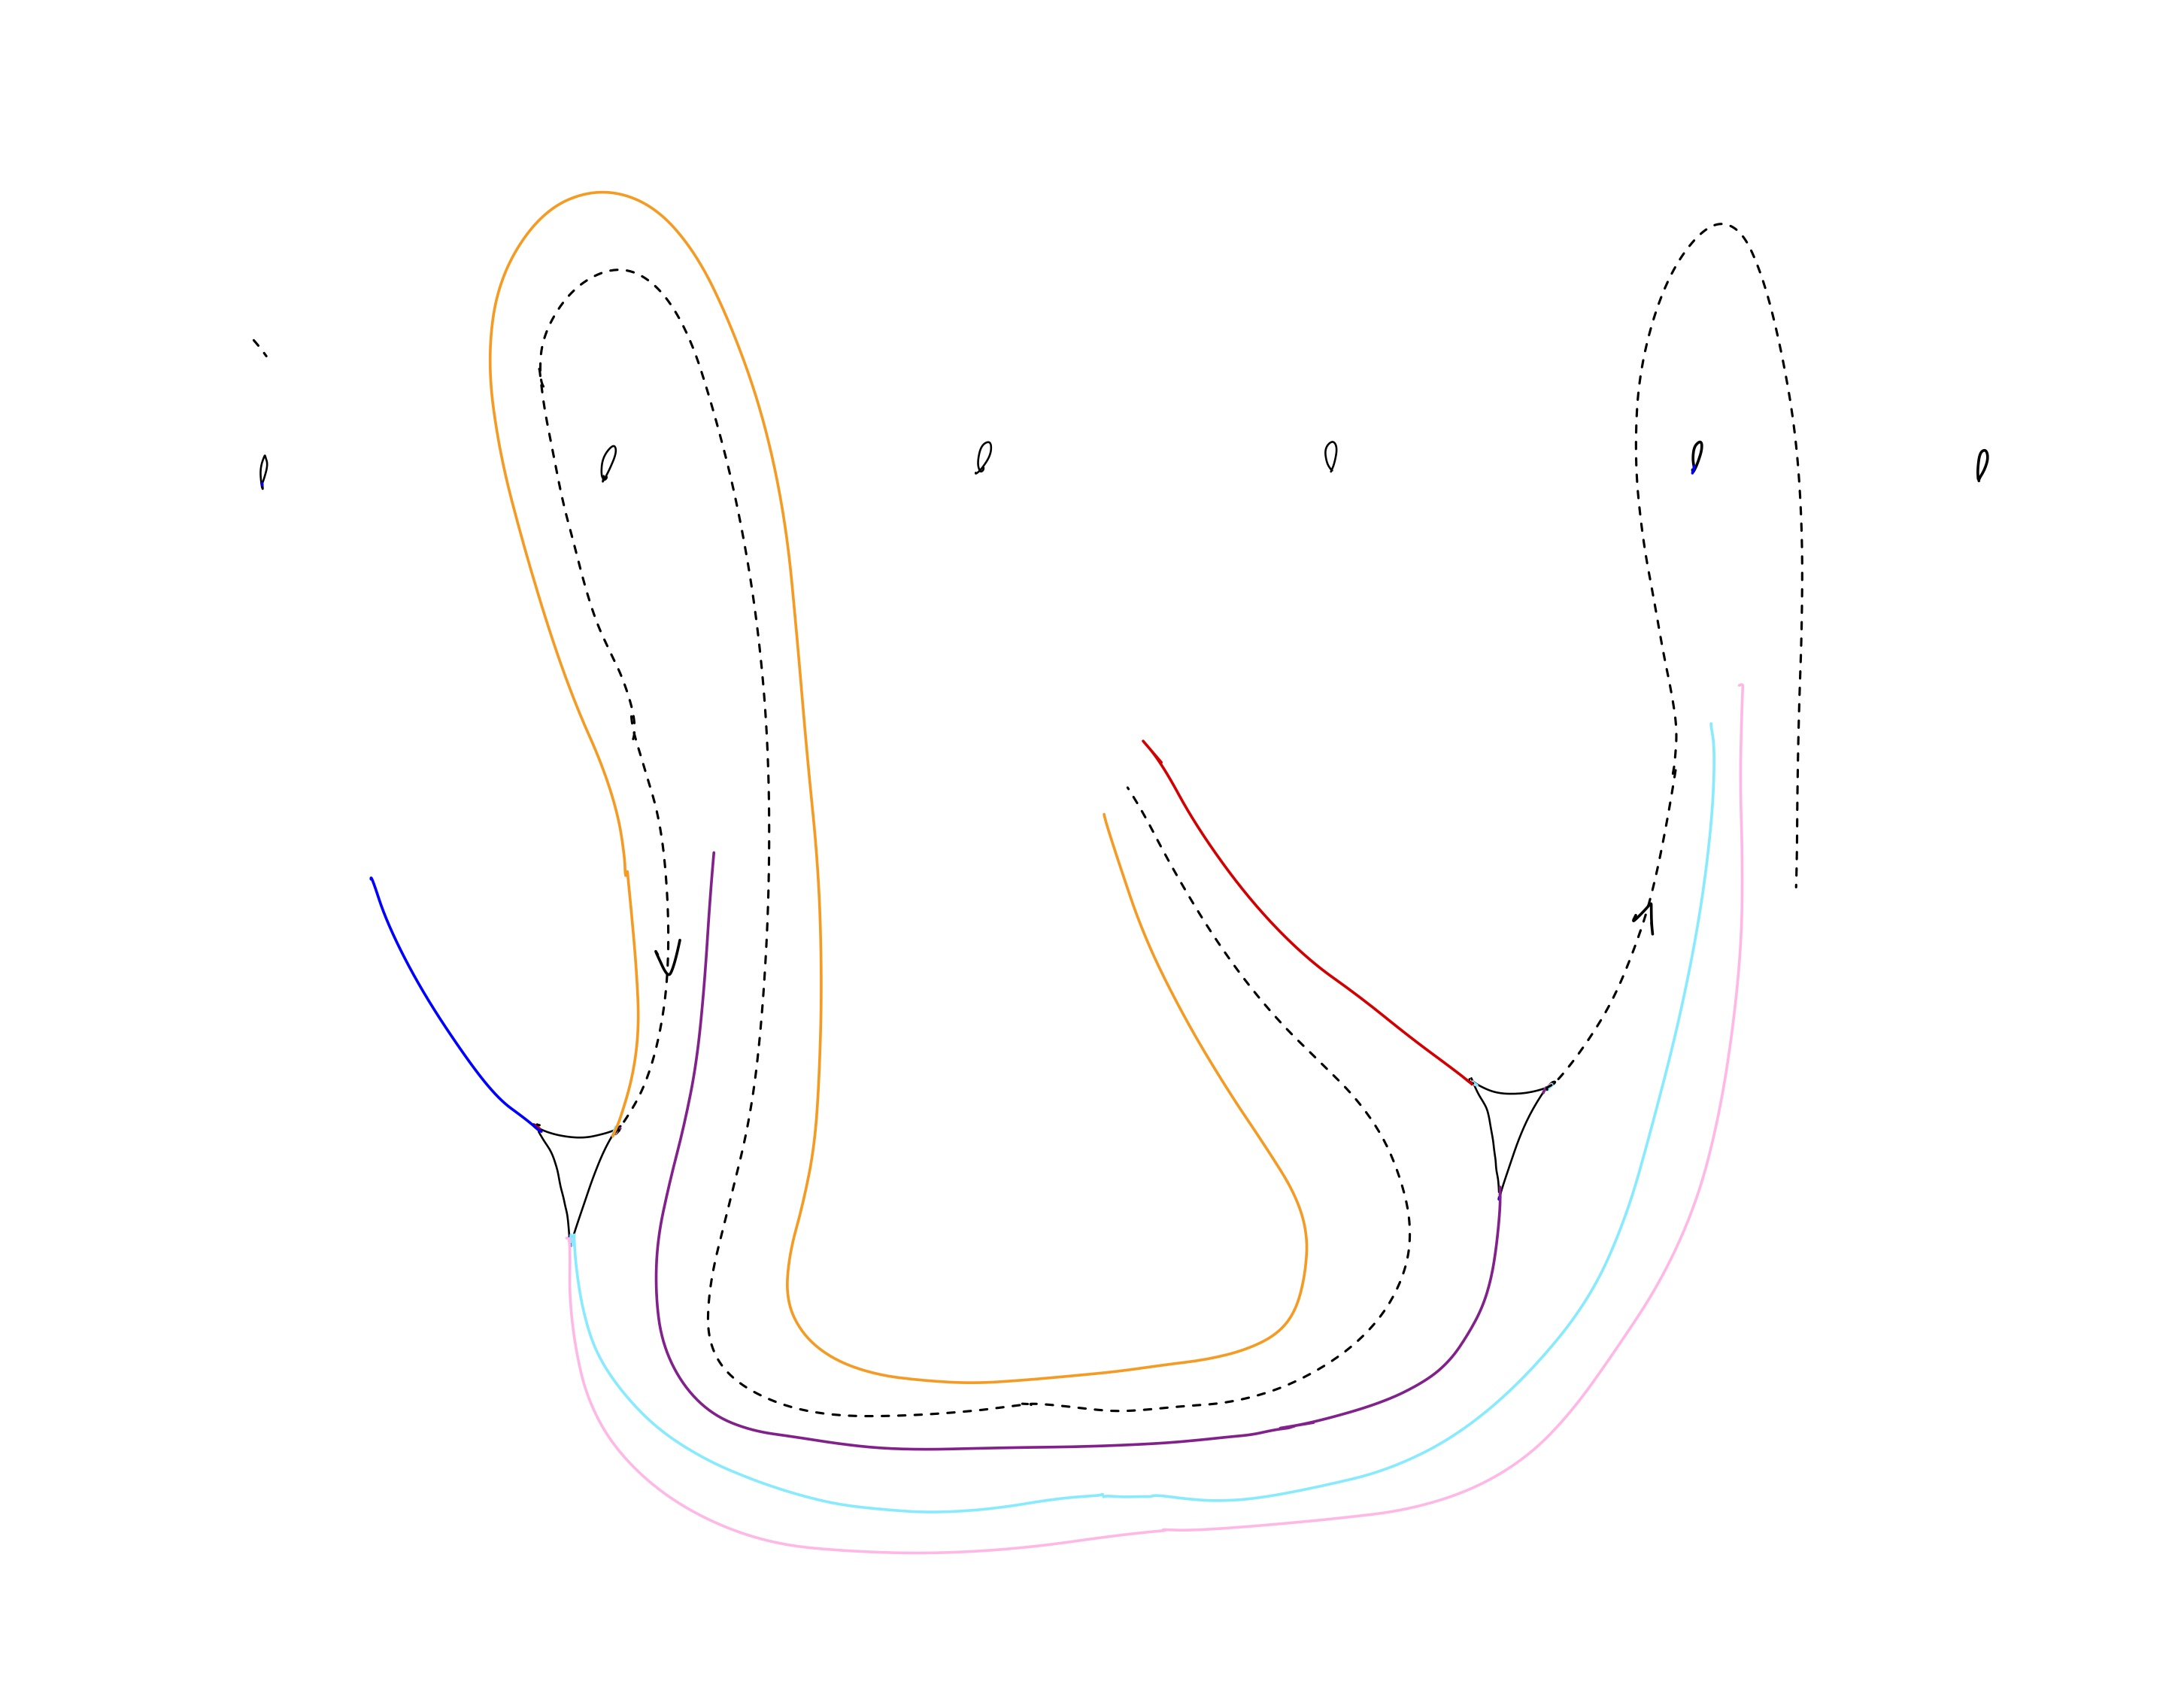
\includegraphics[width=\linewidth]{figures_case_analysis/track17_case_analysis/MMU-04.jpg}
    \caption{MMU4}
    \label{fig:MMU4}
\end{figure}

\begin{figure}[ht]
    \centering
    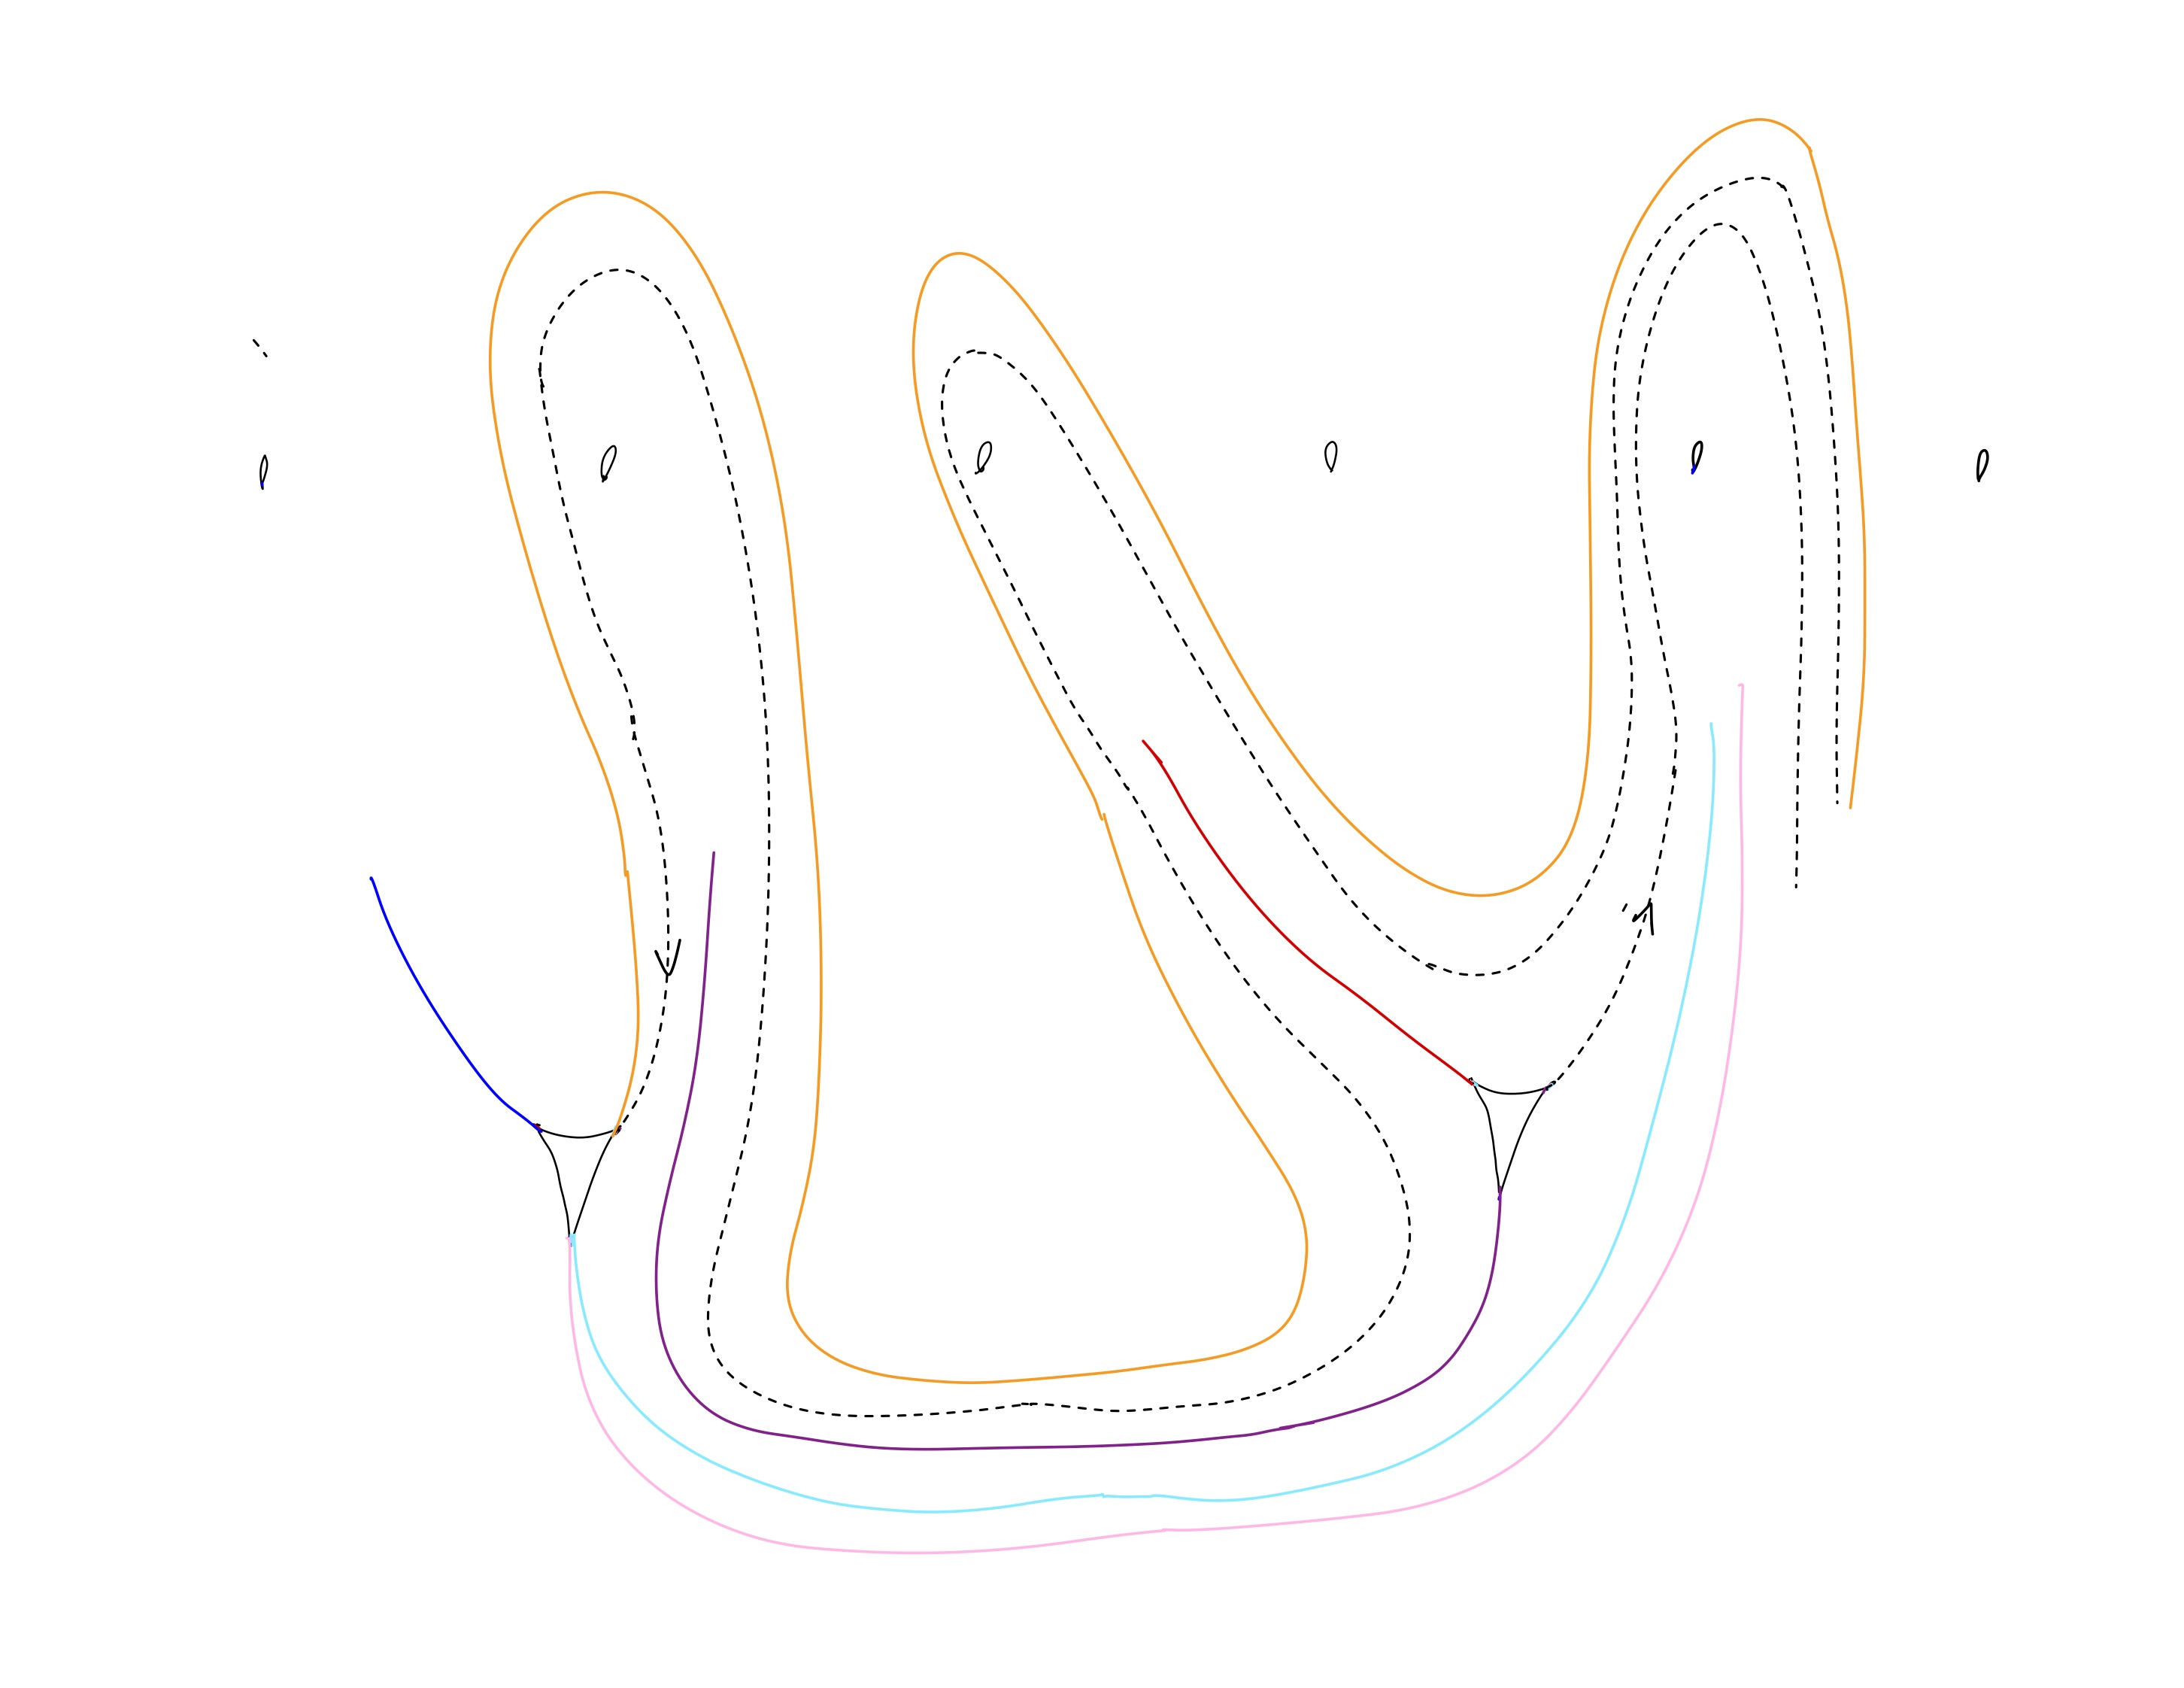
\includegraphics[width=\linewidth]{figures_case_analysis/track17_case_analysis/MMU-05.jpg}
    \caption{MMU5}
    \label{fig:MMU5}
\end{figure}

\begin{figure}[ht]
    \centering
    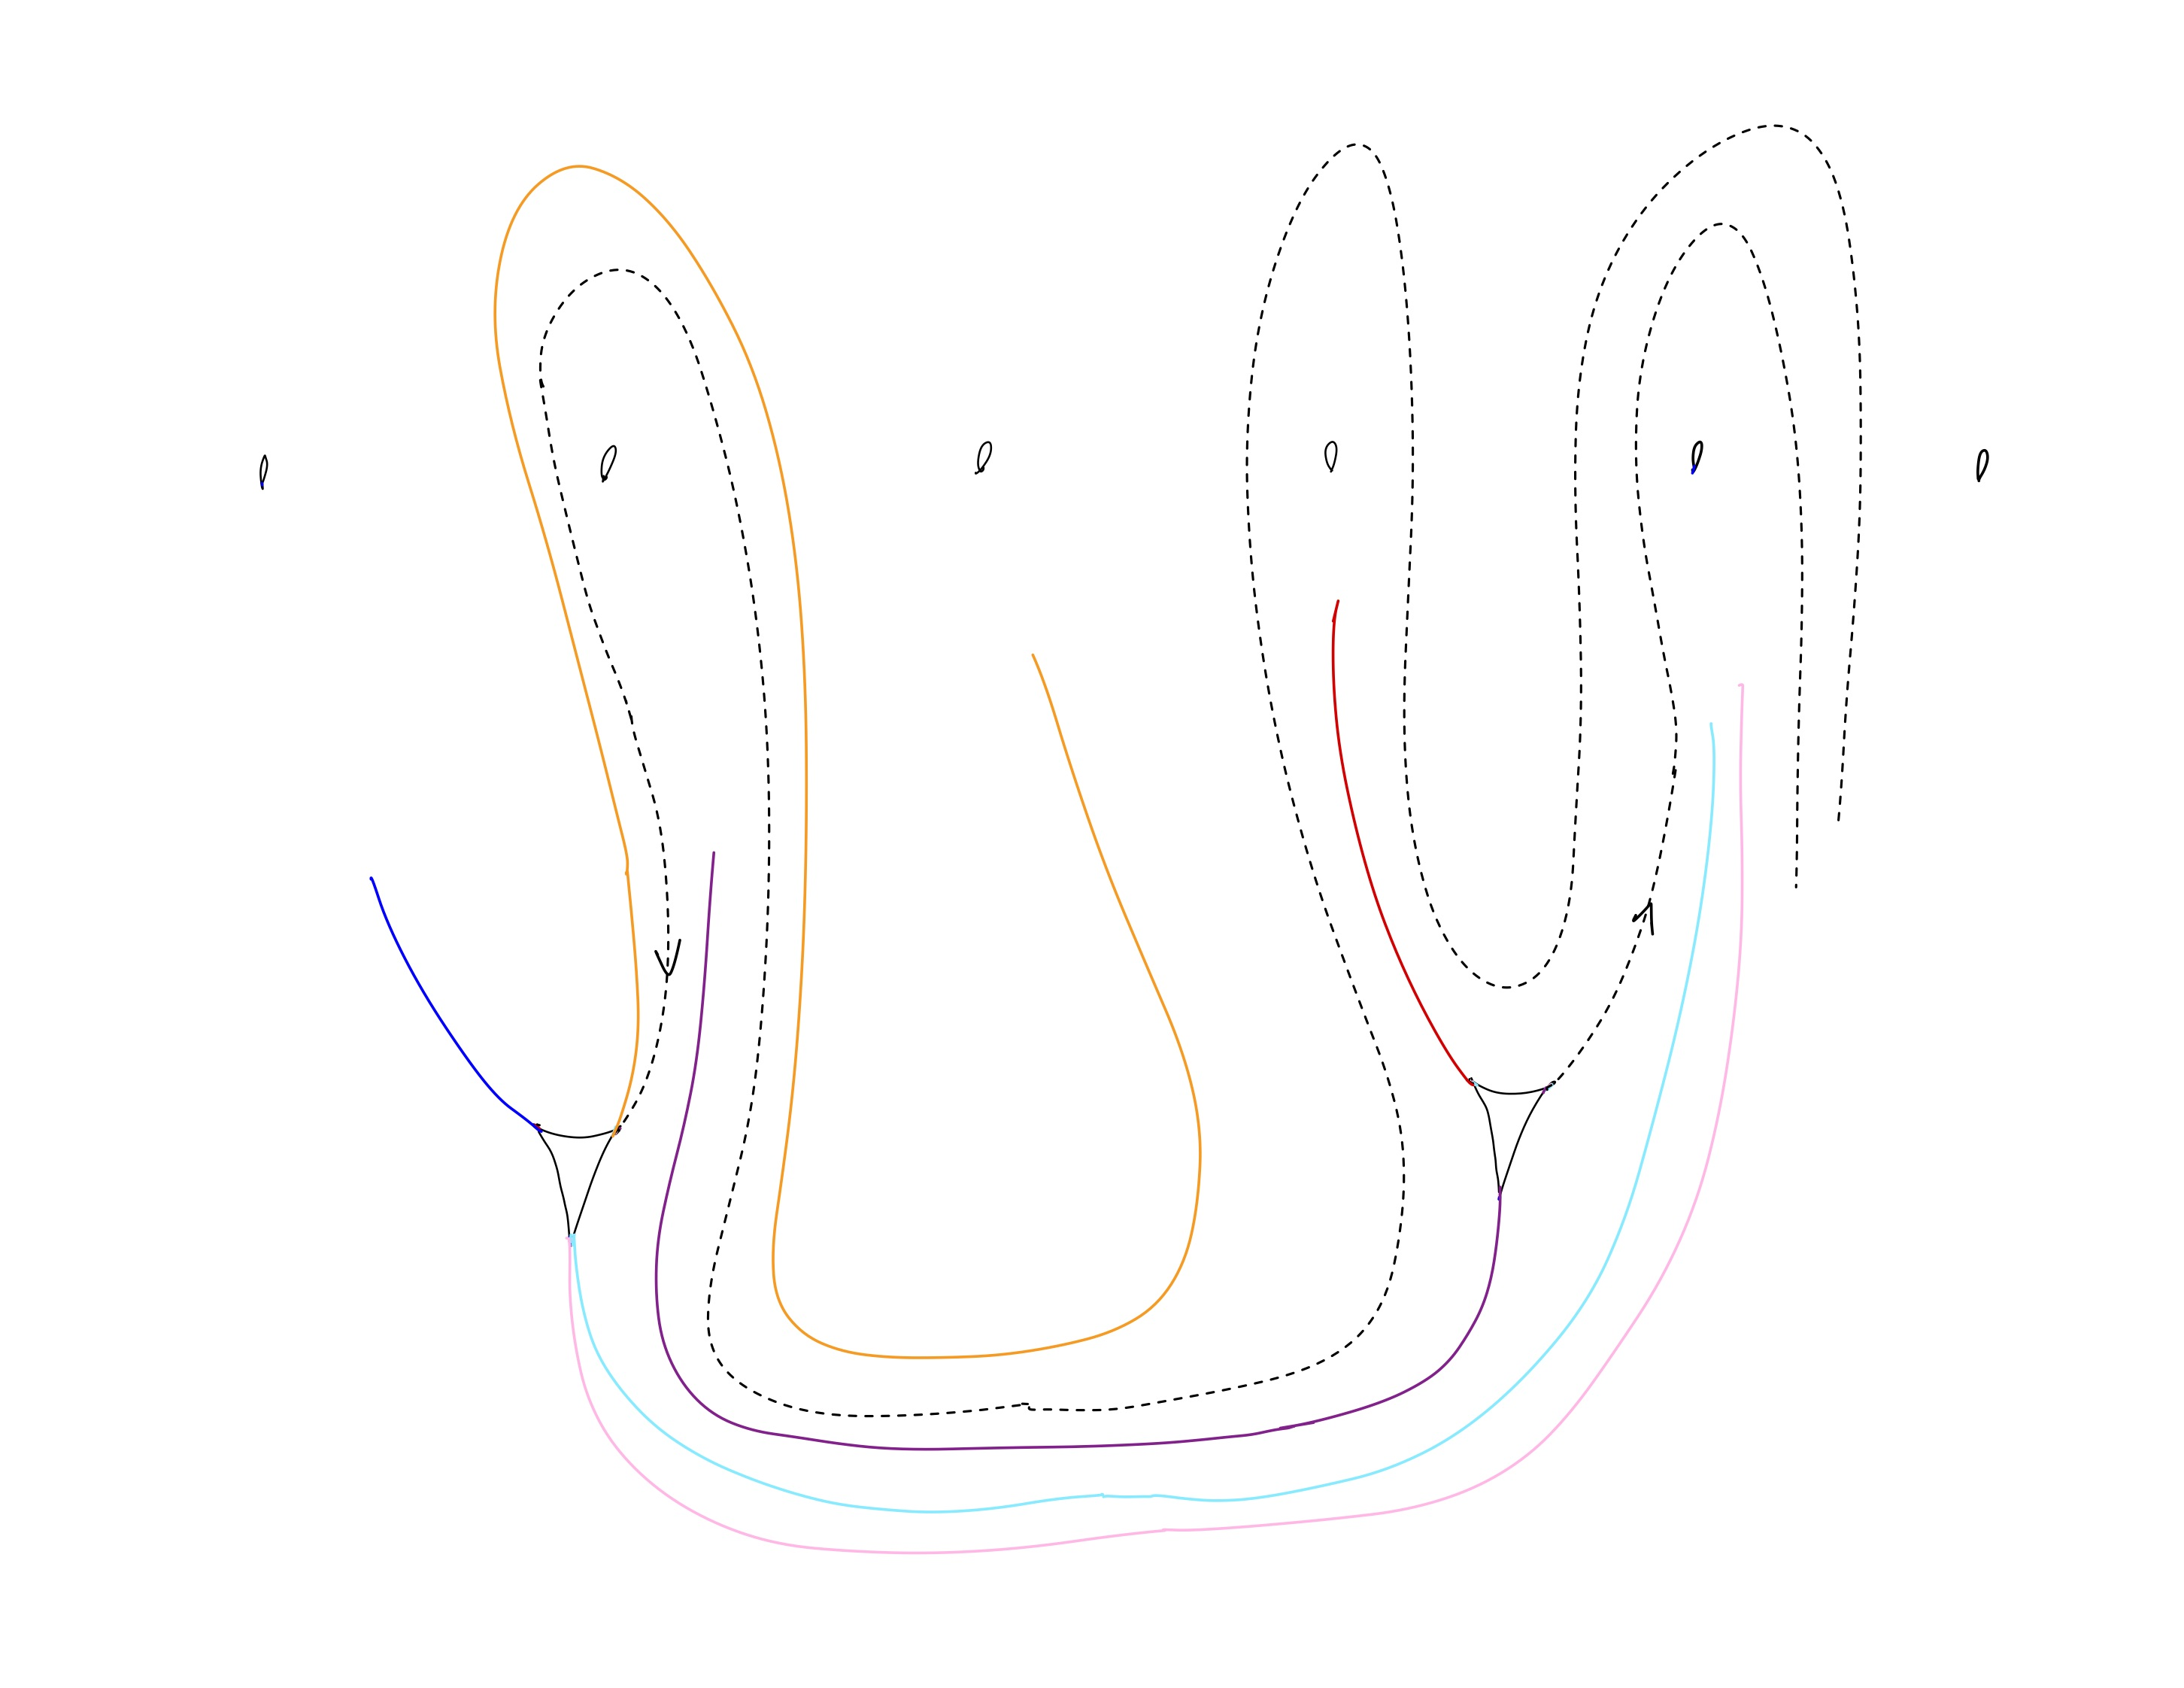
\includegraphics[width=\linewidth]{figures_case_analysis/track17_case_analysis/MMU-06.jpg}
    \caption{MMU6}
    \label{fig:MMU6}
\end{figure}

\begin{figure}[ht]
    \centering
    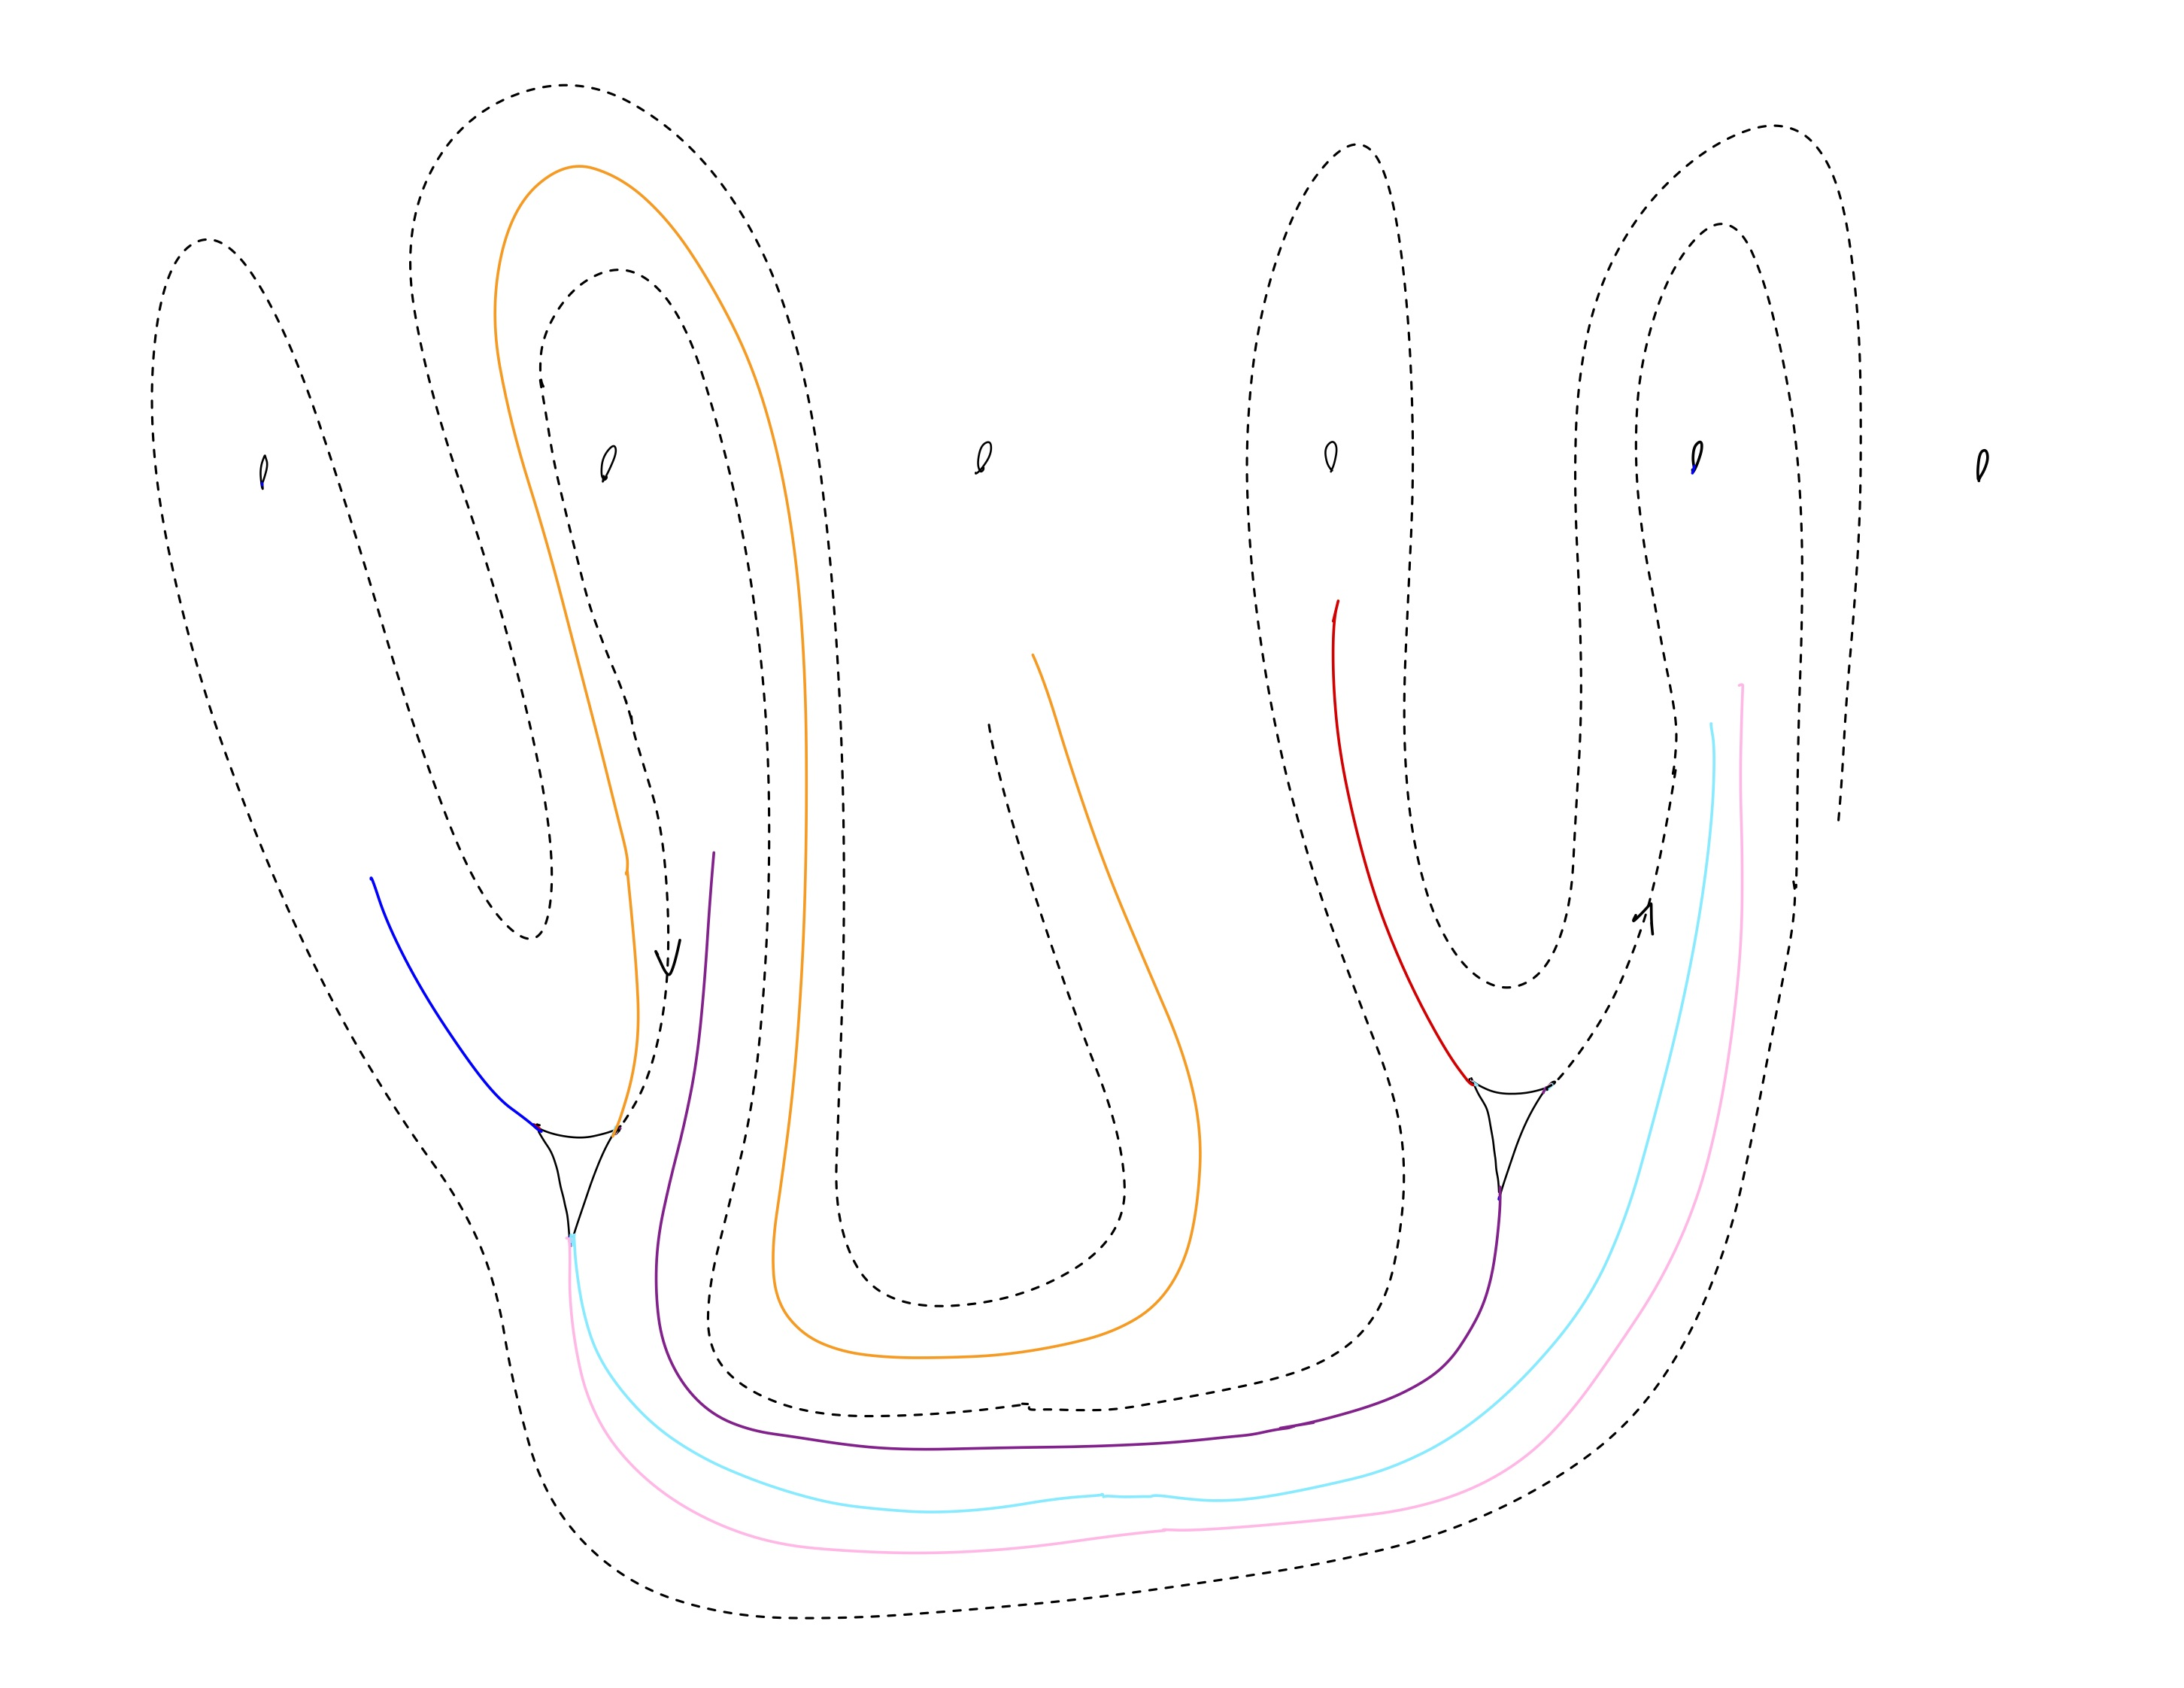
\includegraphics[width=\linewidth]{figures_case_analysis/track17_case_analysis/MMU-07.jpg}
    \caption{MMU7}
    \label{fig:MMU7}
\end{figure}

\begin{figure}[ht]
    \centering
    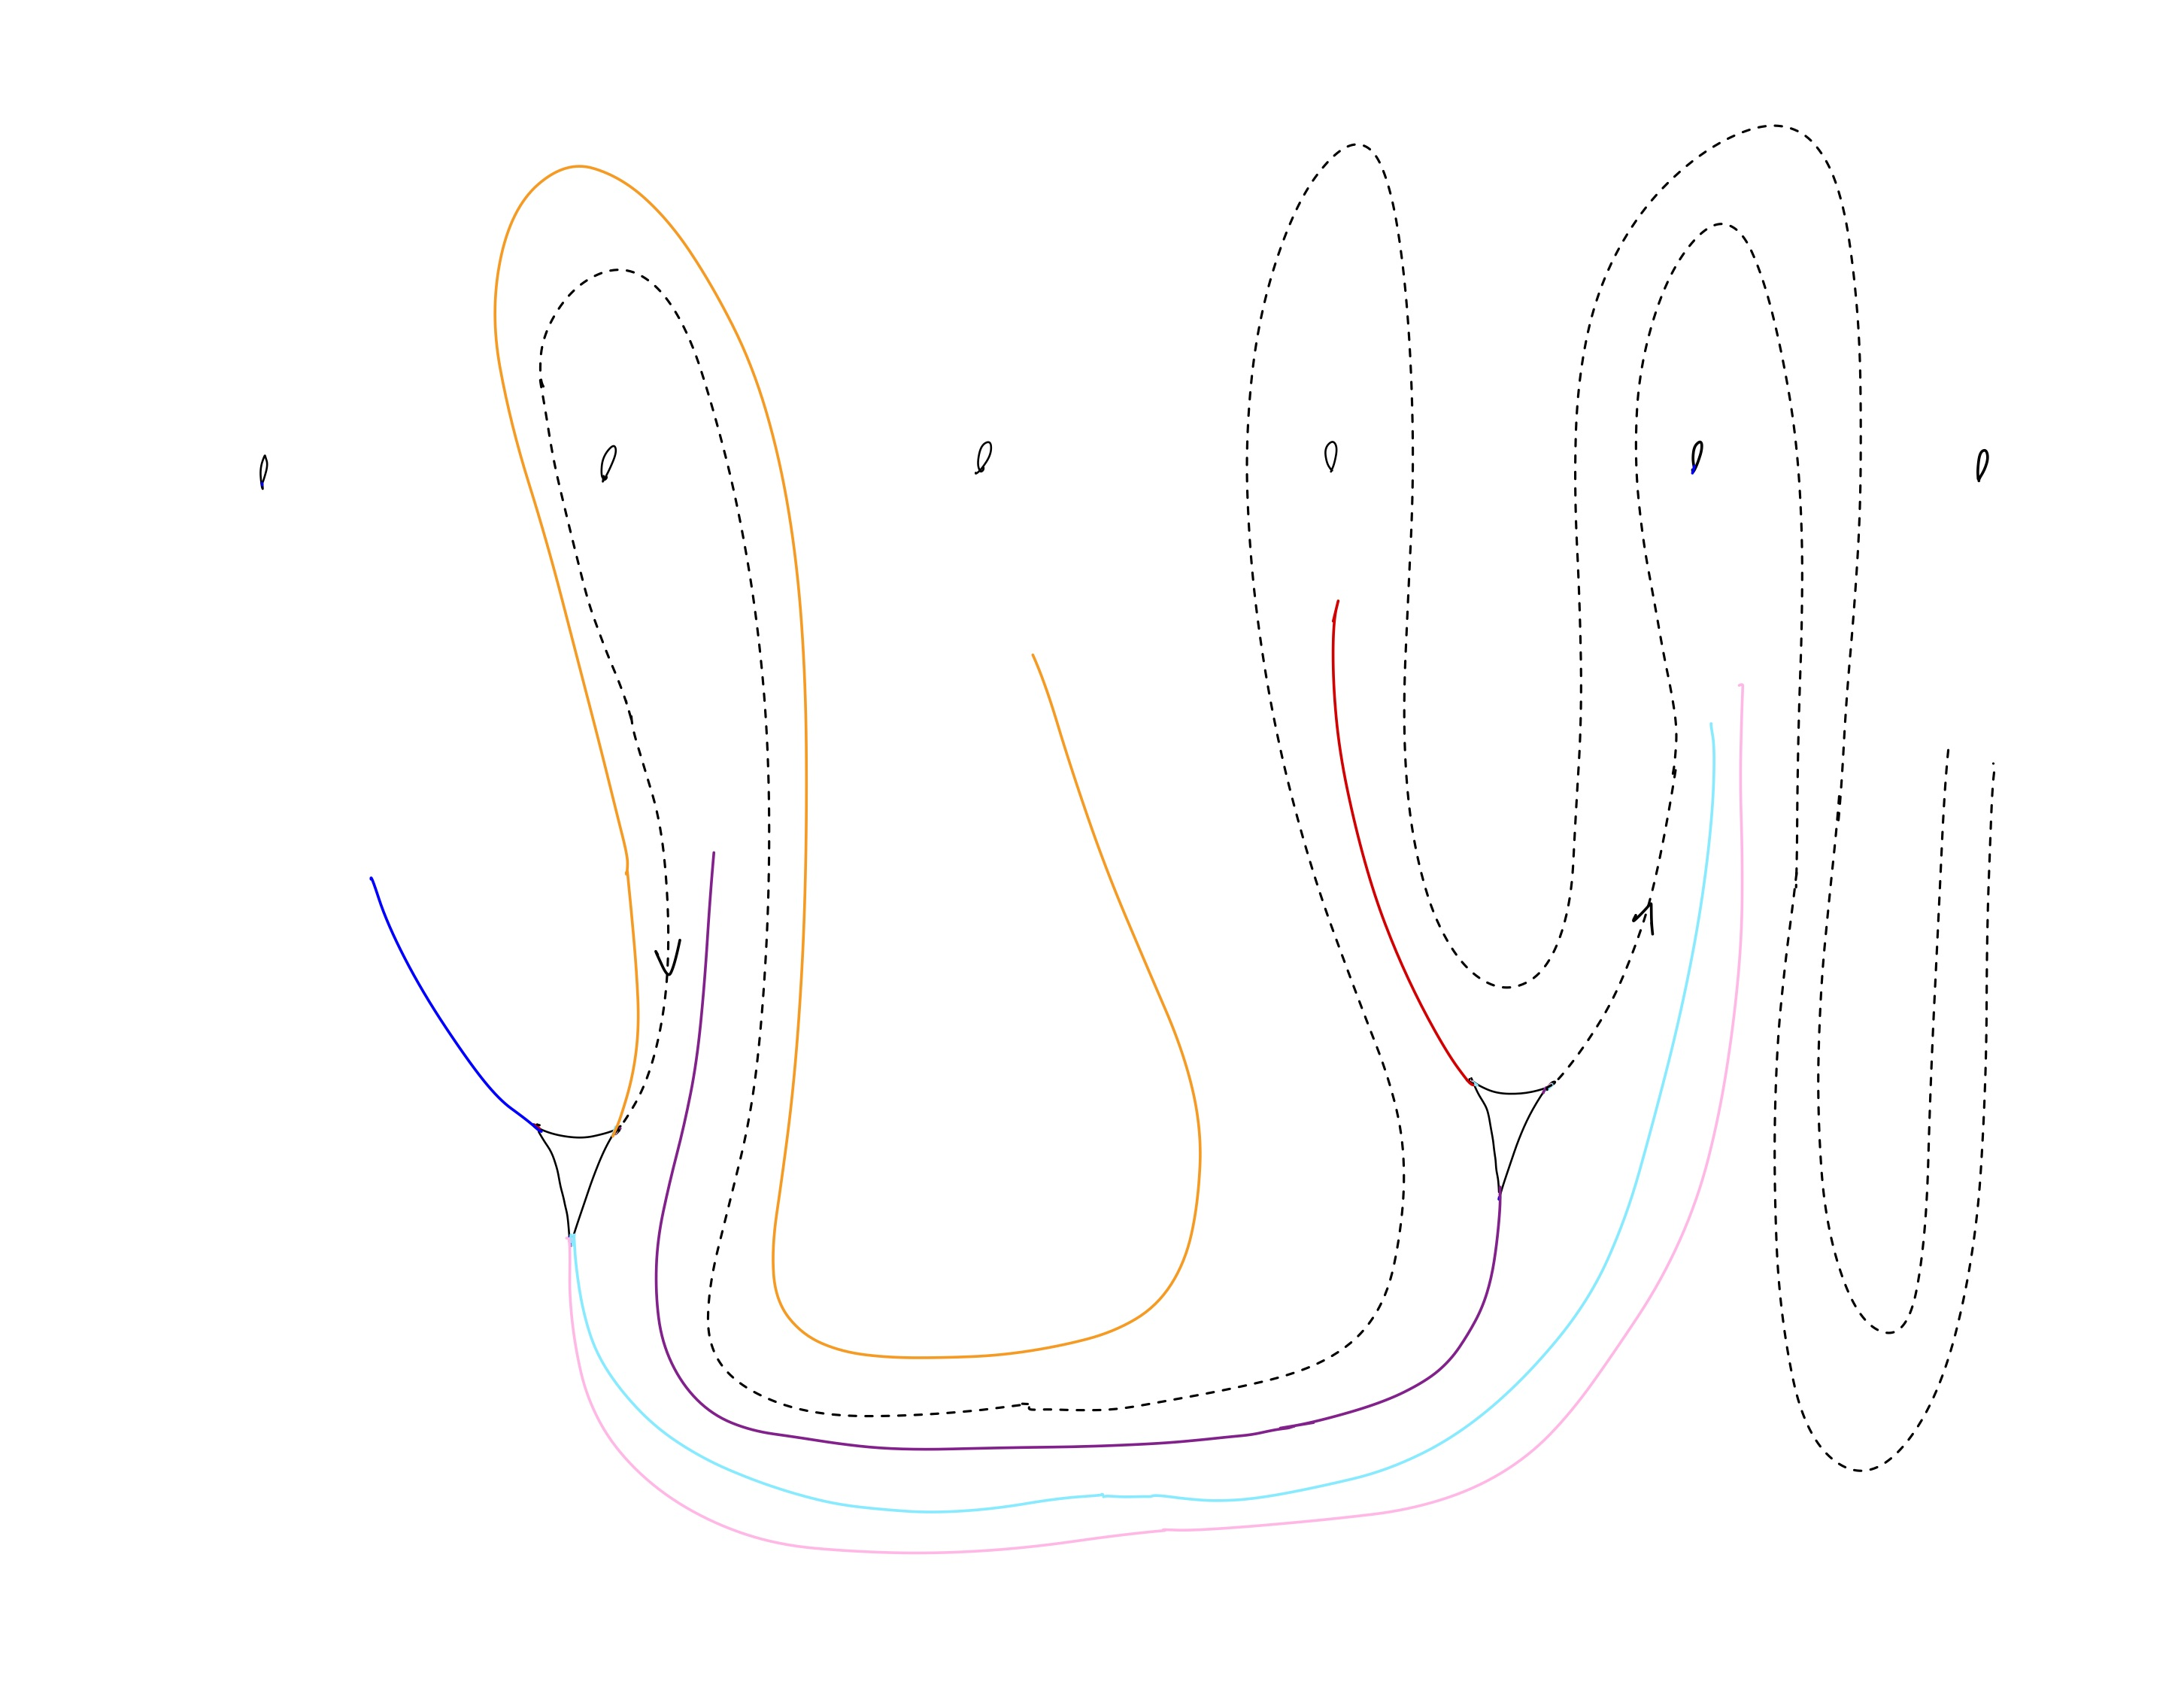
\includegraphics[width=\linewidth]{figures_case_analysis/track17_case_analysis/MMU-08.jpg}
    \caption{MMU8}
    \label{fig:MMU8}
\end{figure}

\begin{figure}[ht]
    \centering
    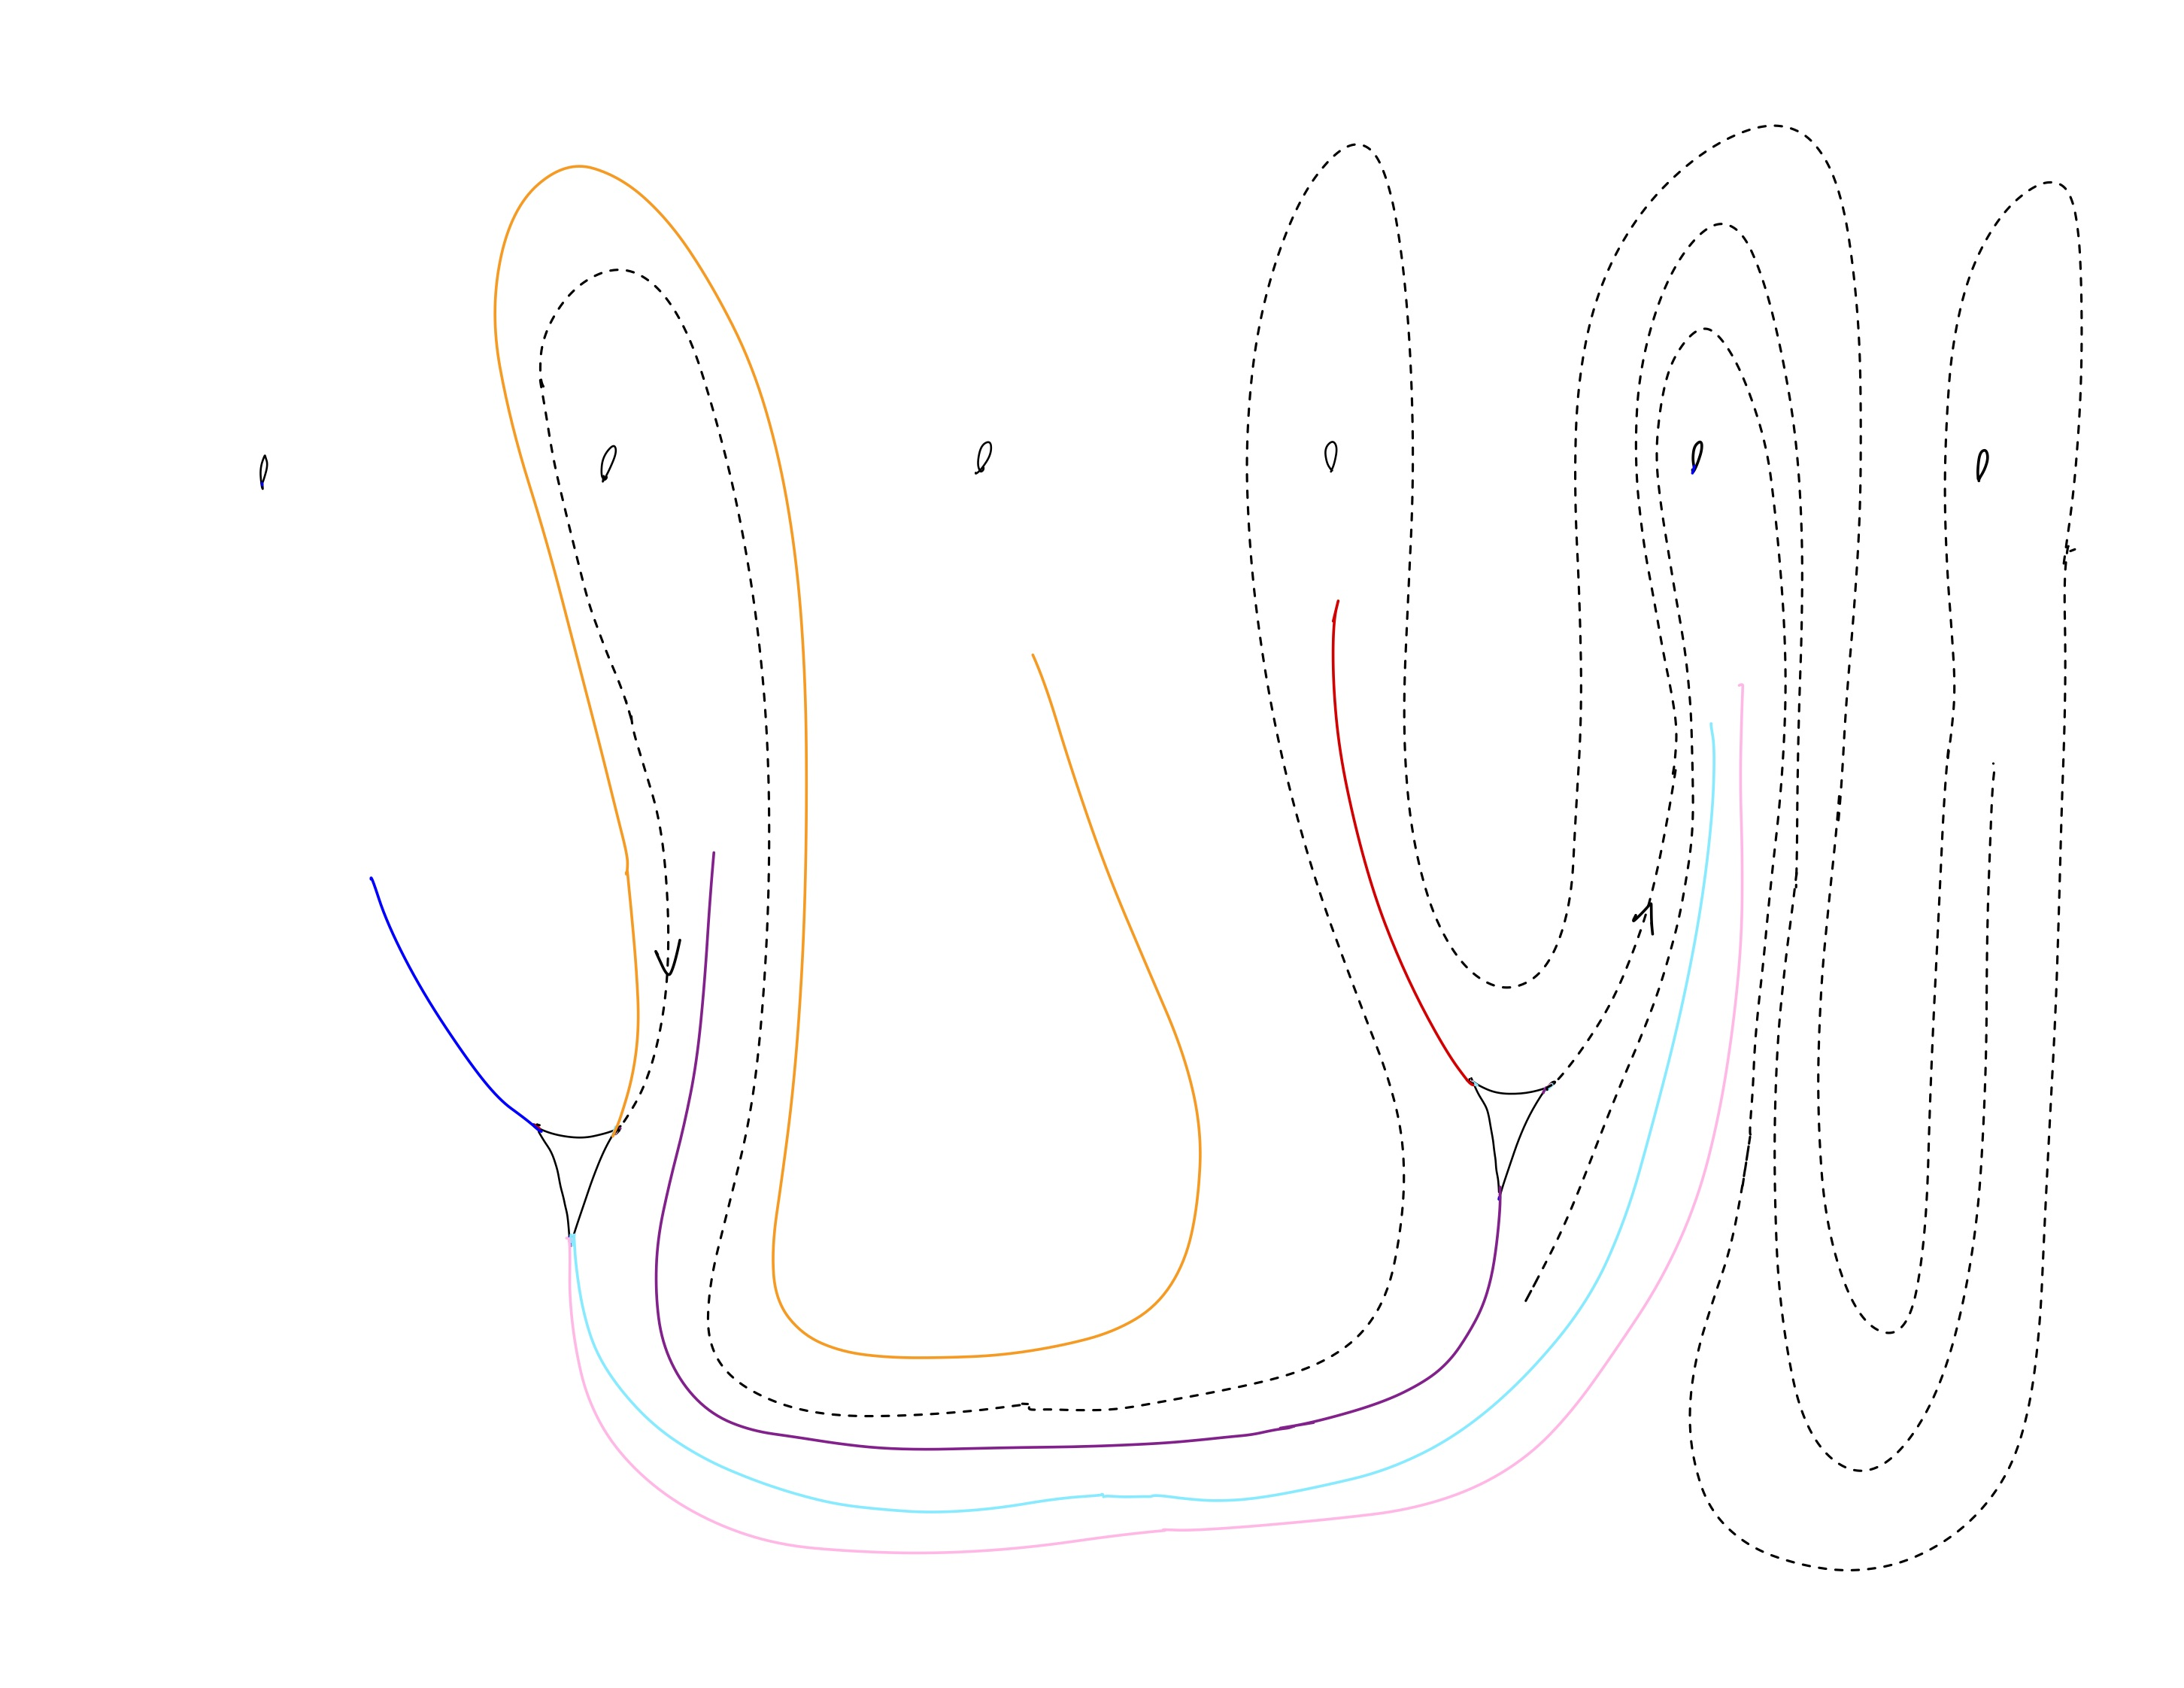
\includegraphics[width=\linewidth]{figures_case_analysis/track17_case_analysis/MMU-09.jpg}
    \caption{MMU9}
    \label{fig:MMU9}
\end{figure}

\begin{figure}[ht]
    \centering
    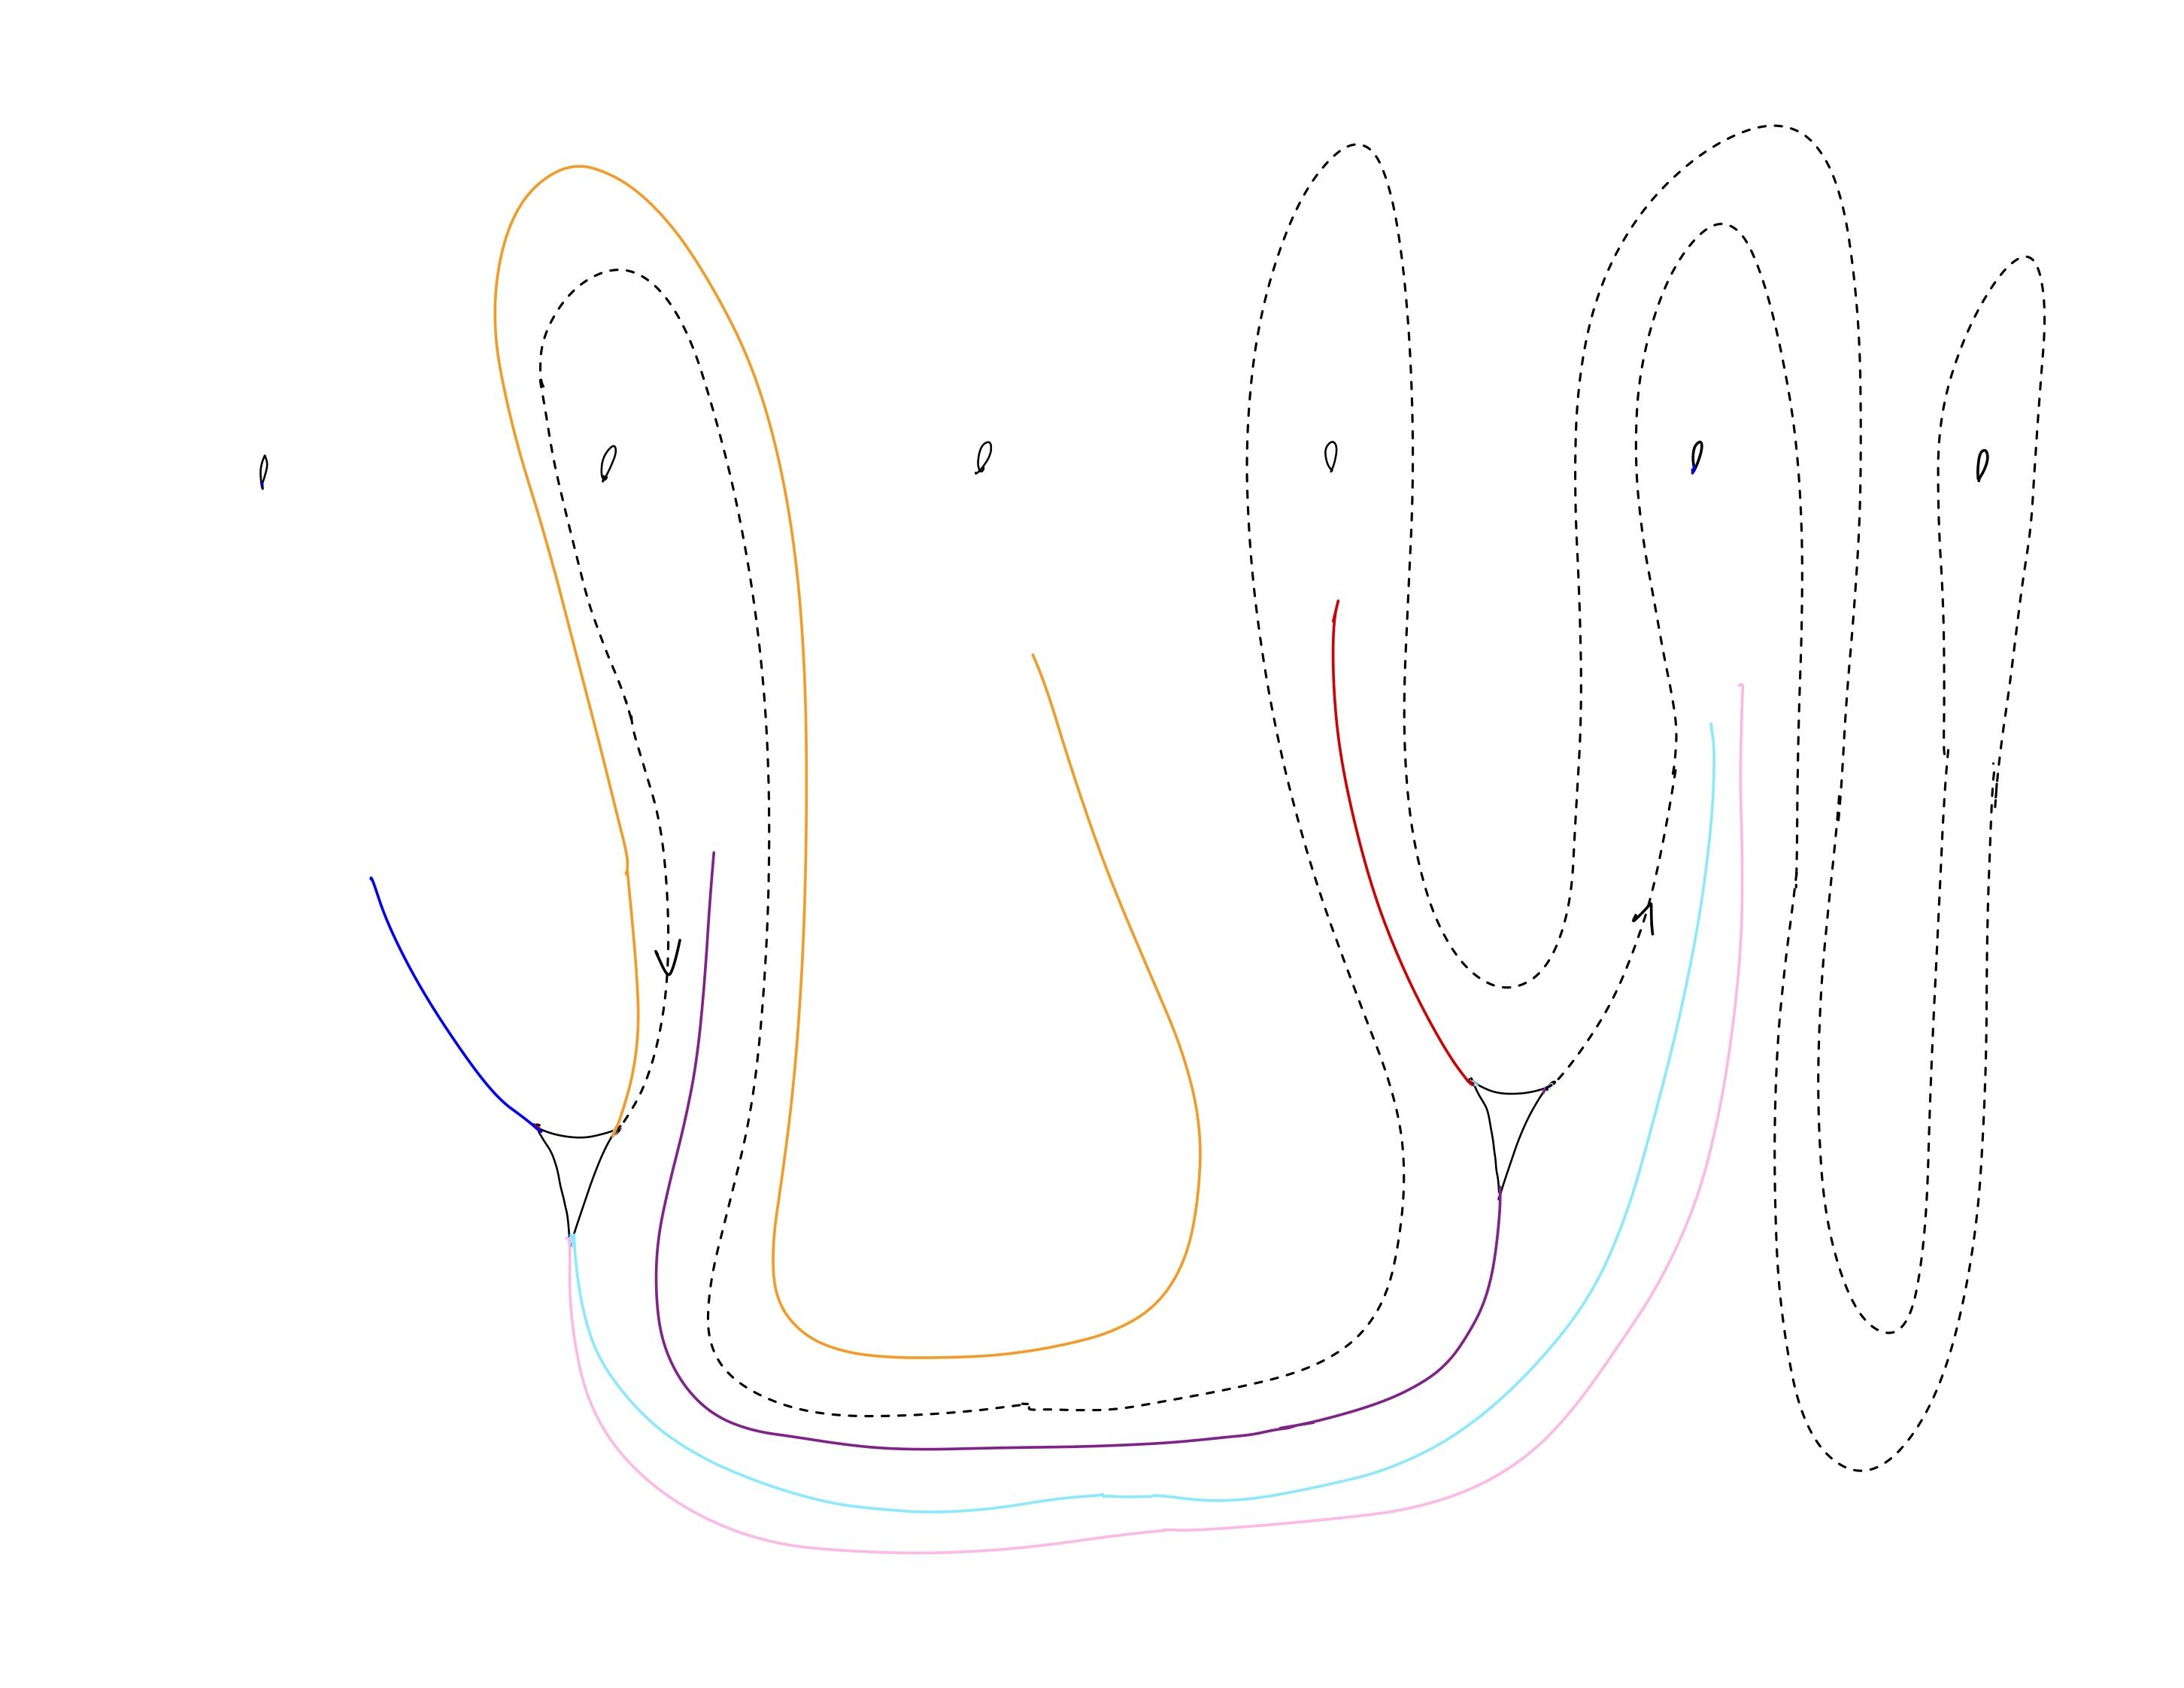
\includegraphics[width=\linewidth]{figures_case_analysis/track17_case_analysis/MMU-10.jpg}
    \caption{MMU10}
    \label{fig:MMU10}
\end{figure}

\begin{figure}[ht]
    \centering
    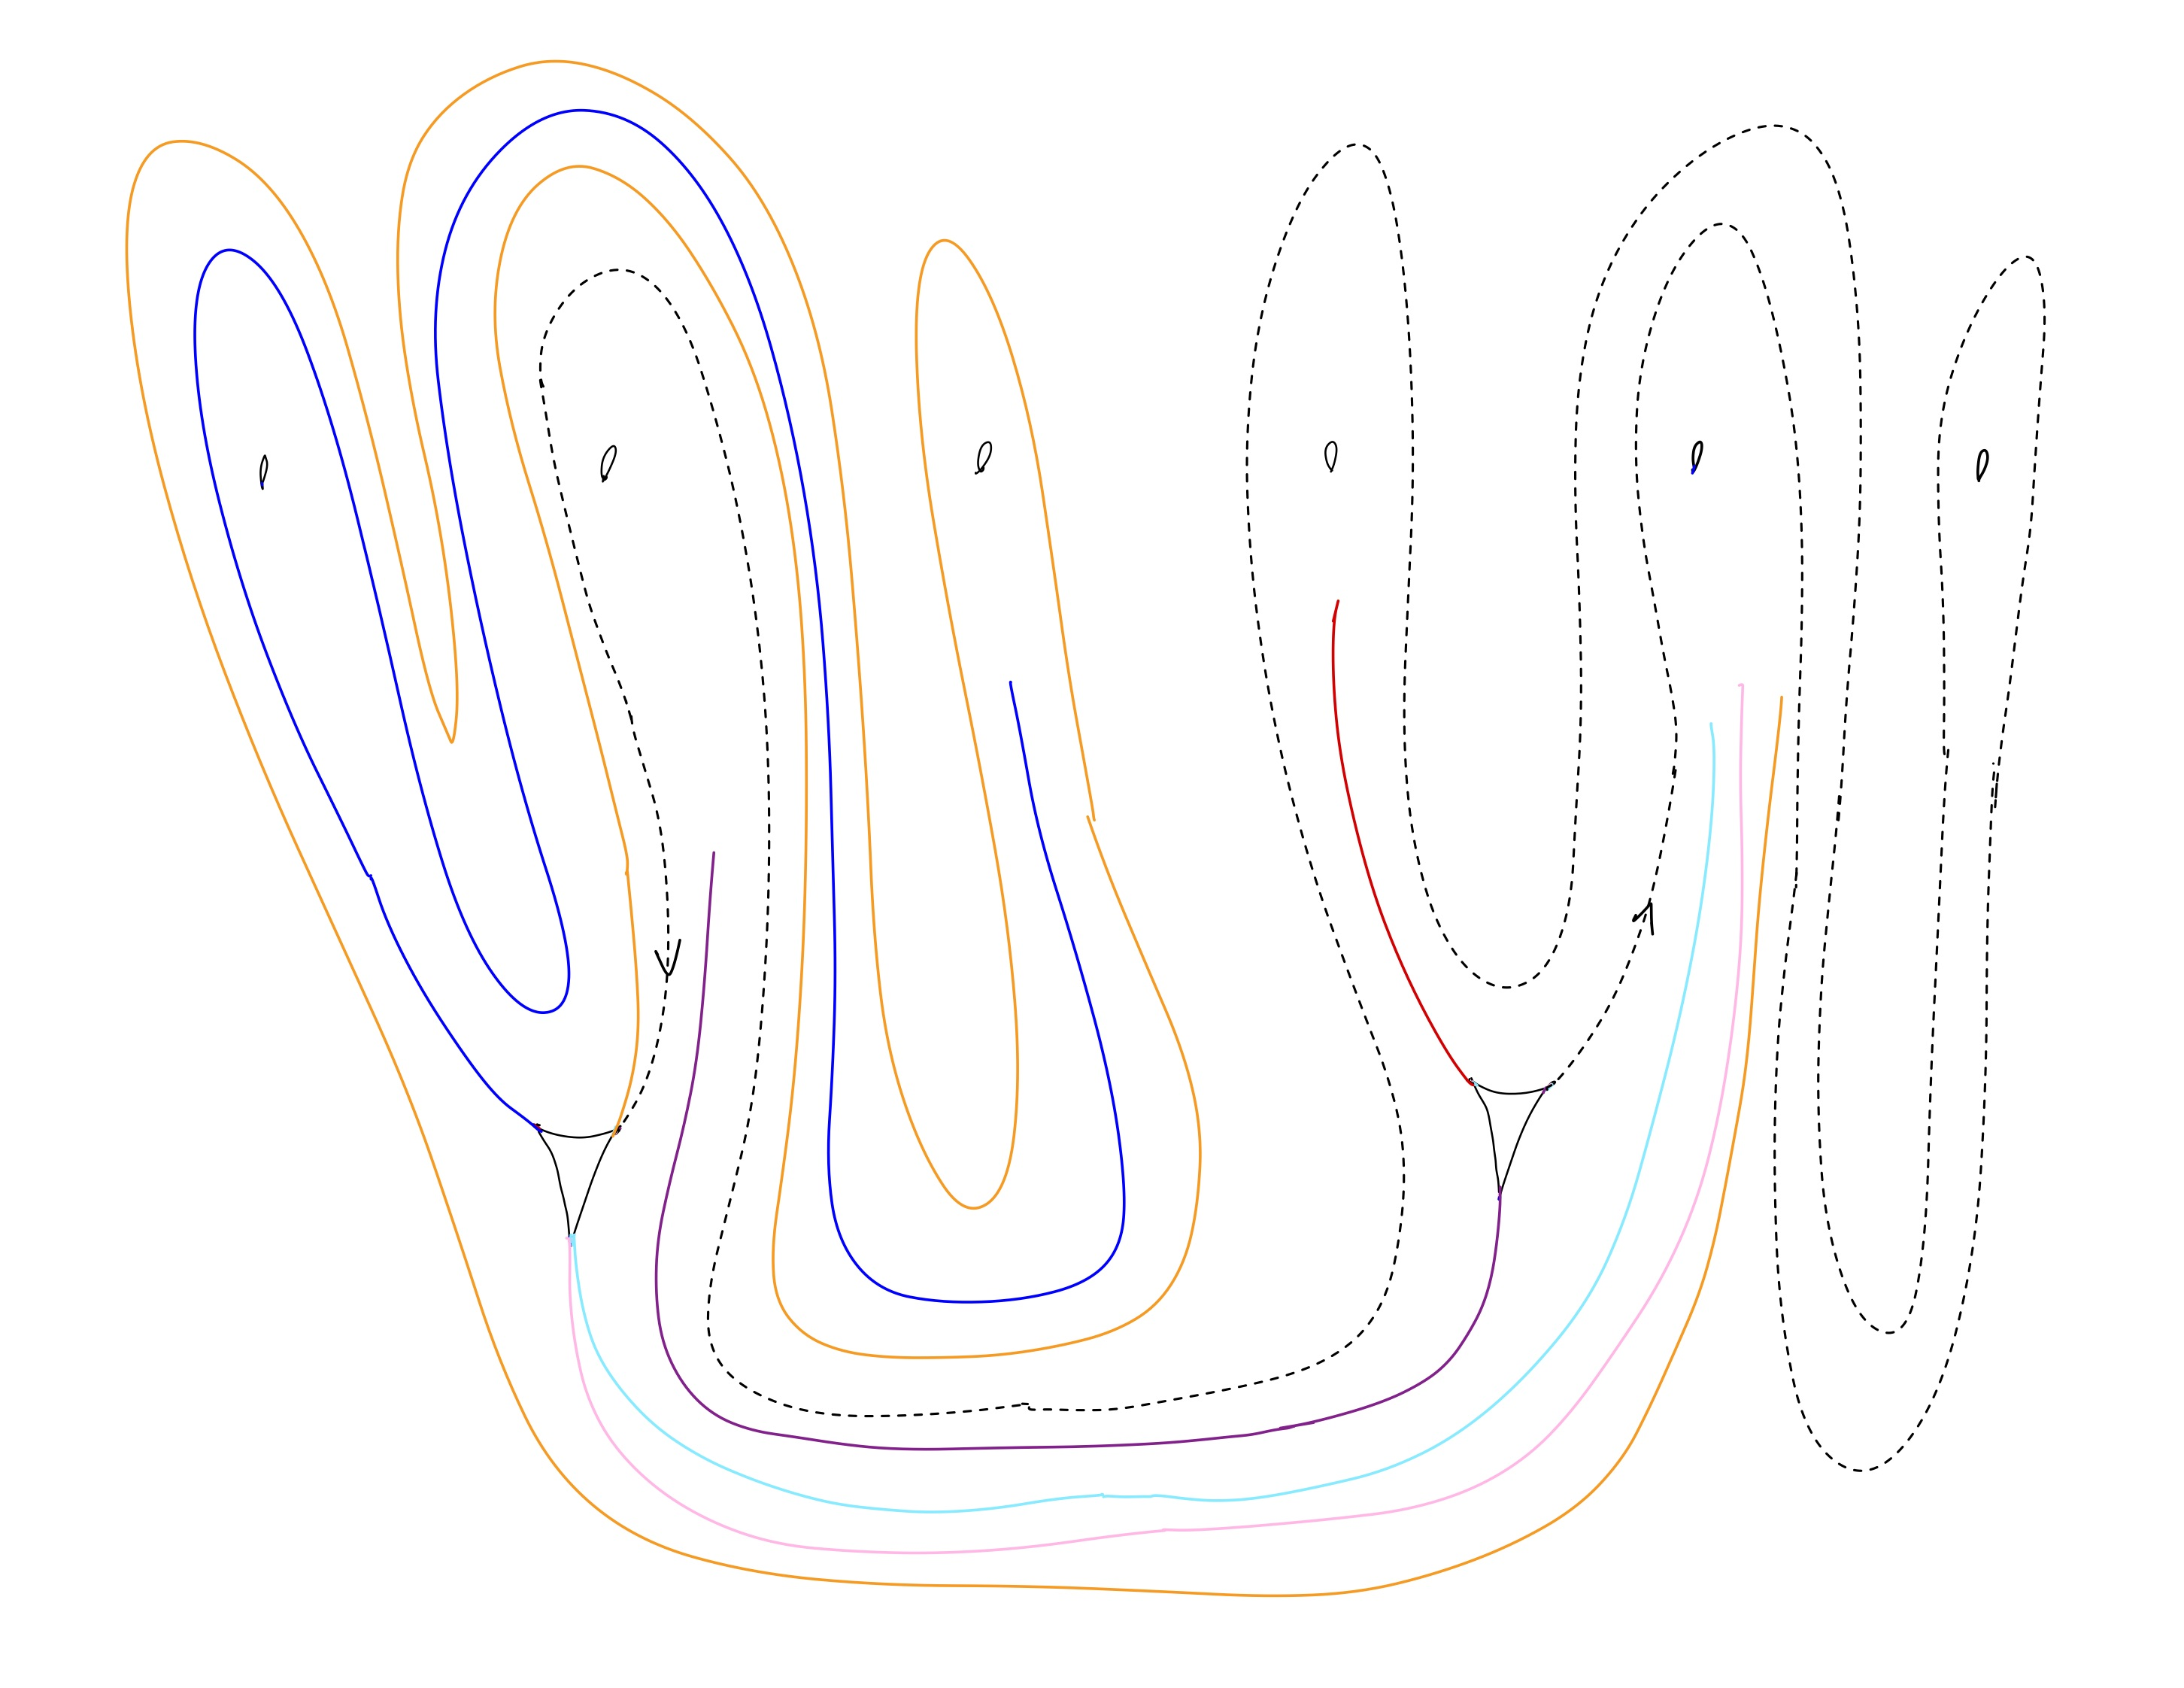
\includegraphics[width=\linewidth]{figures_case_analysis/track17_case_analysis/MMU-11.jpg}
    \caption{MMU11}
    \label{fig:MMU11}
\end{figure}

\begin{figure}[ht]
    \centering
    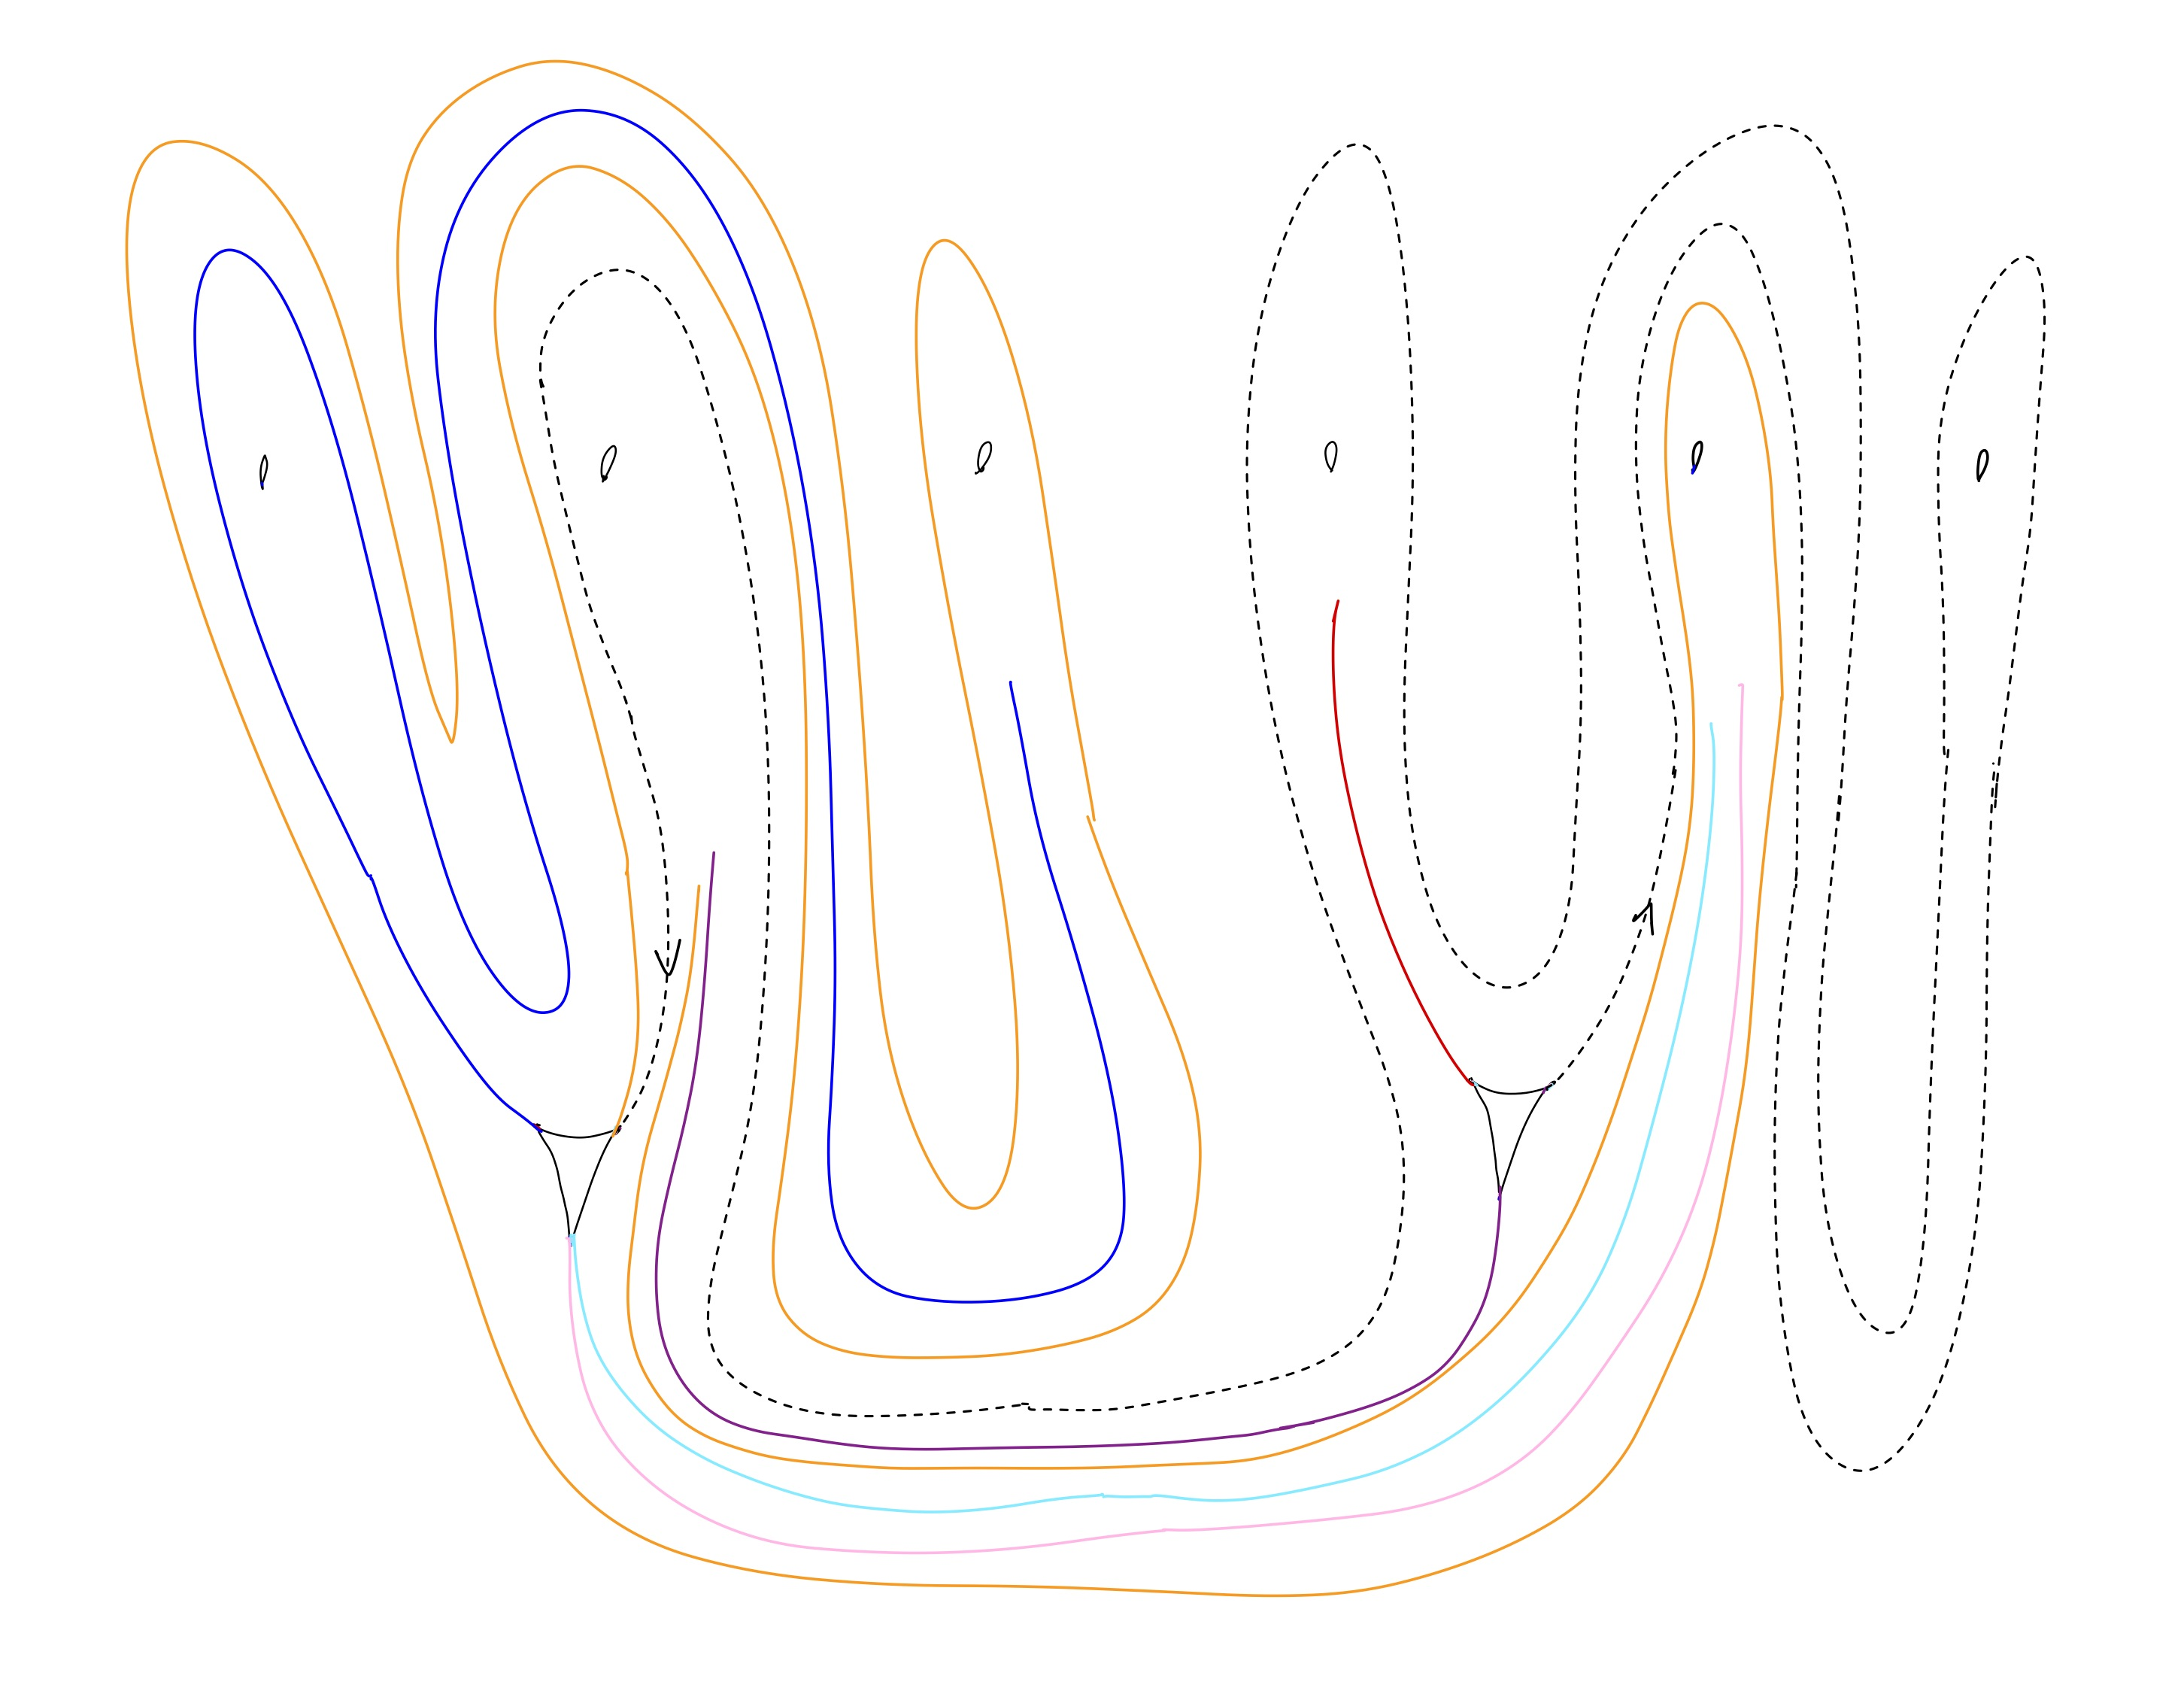
\includegraphics[width=\linewidth]{figures_case_analysis/track17_case_analysis/MMU-12.jpg}
    \caption{MMU12}
    \label{fig:MMU12}
\end{figure}

\begin{figure}[ht]
    \centering
    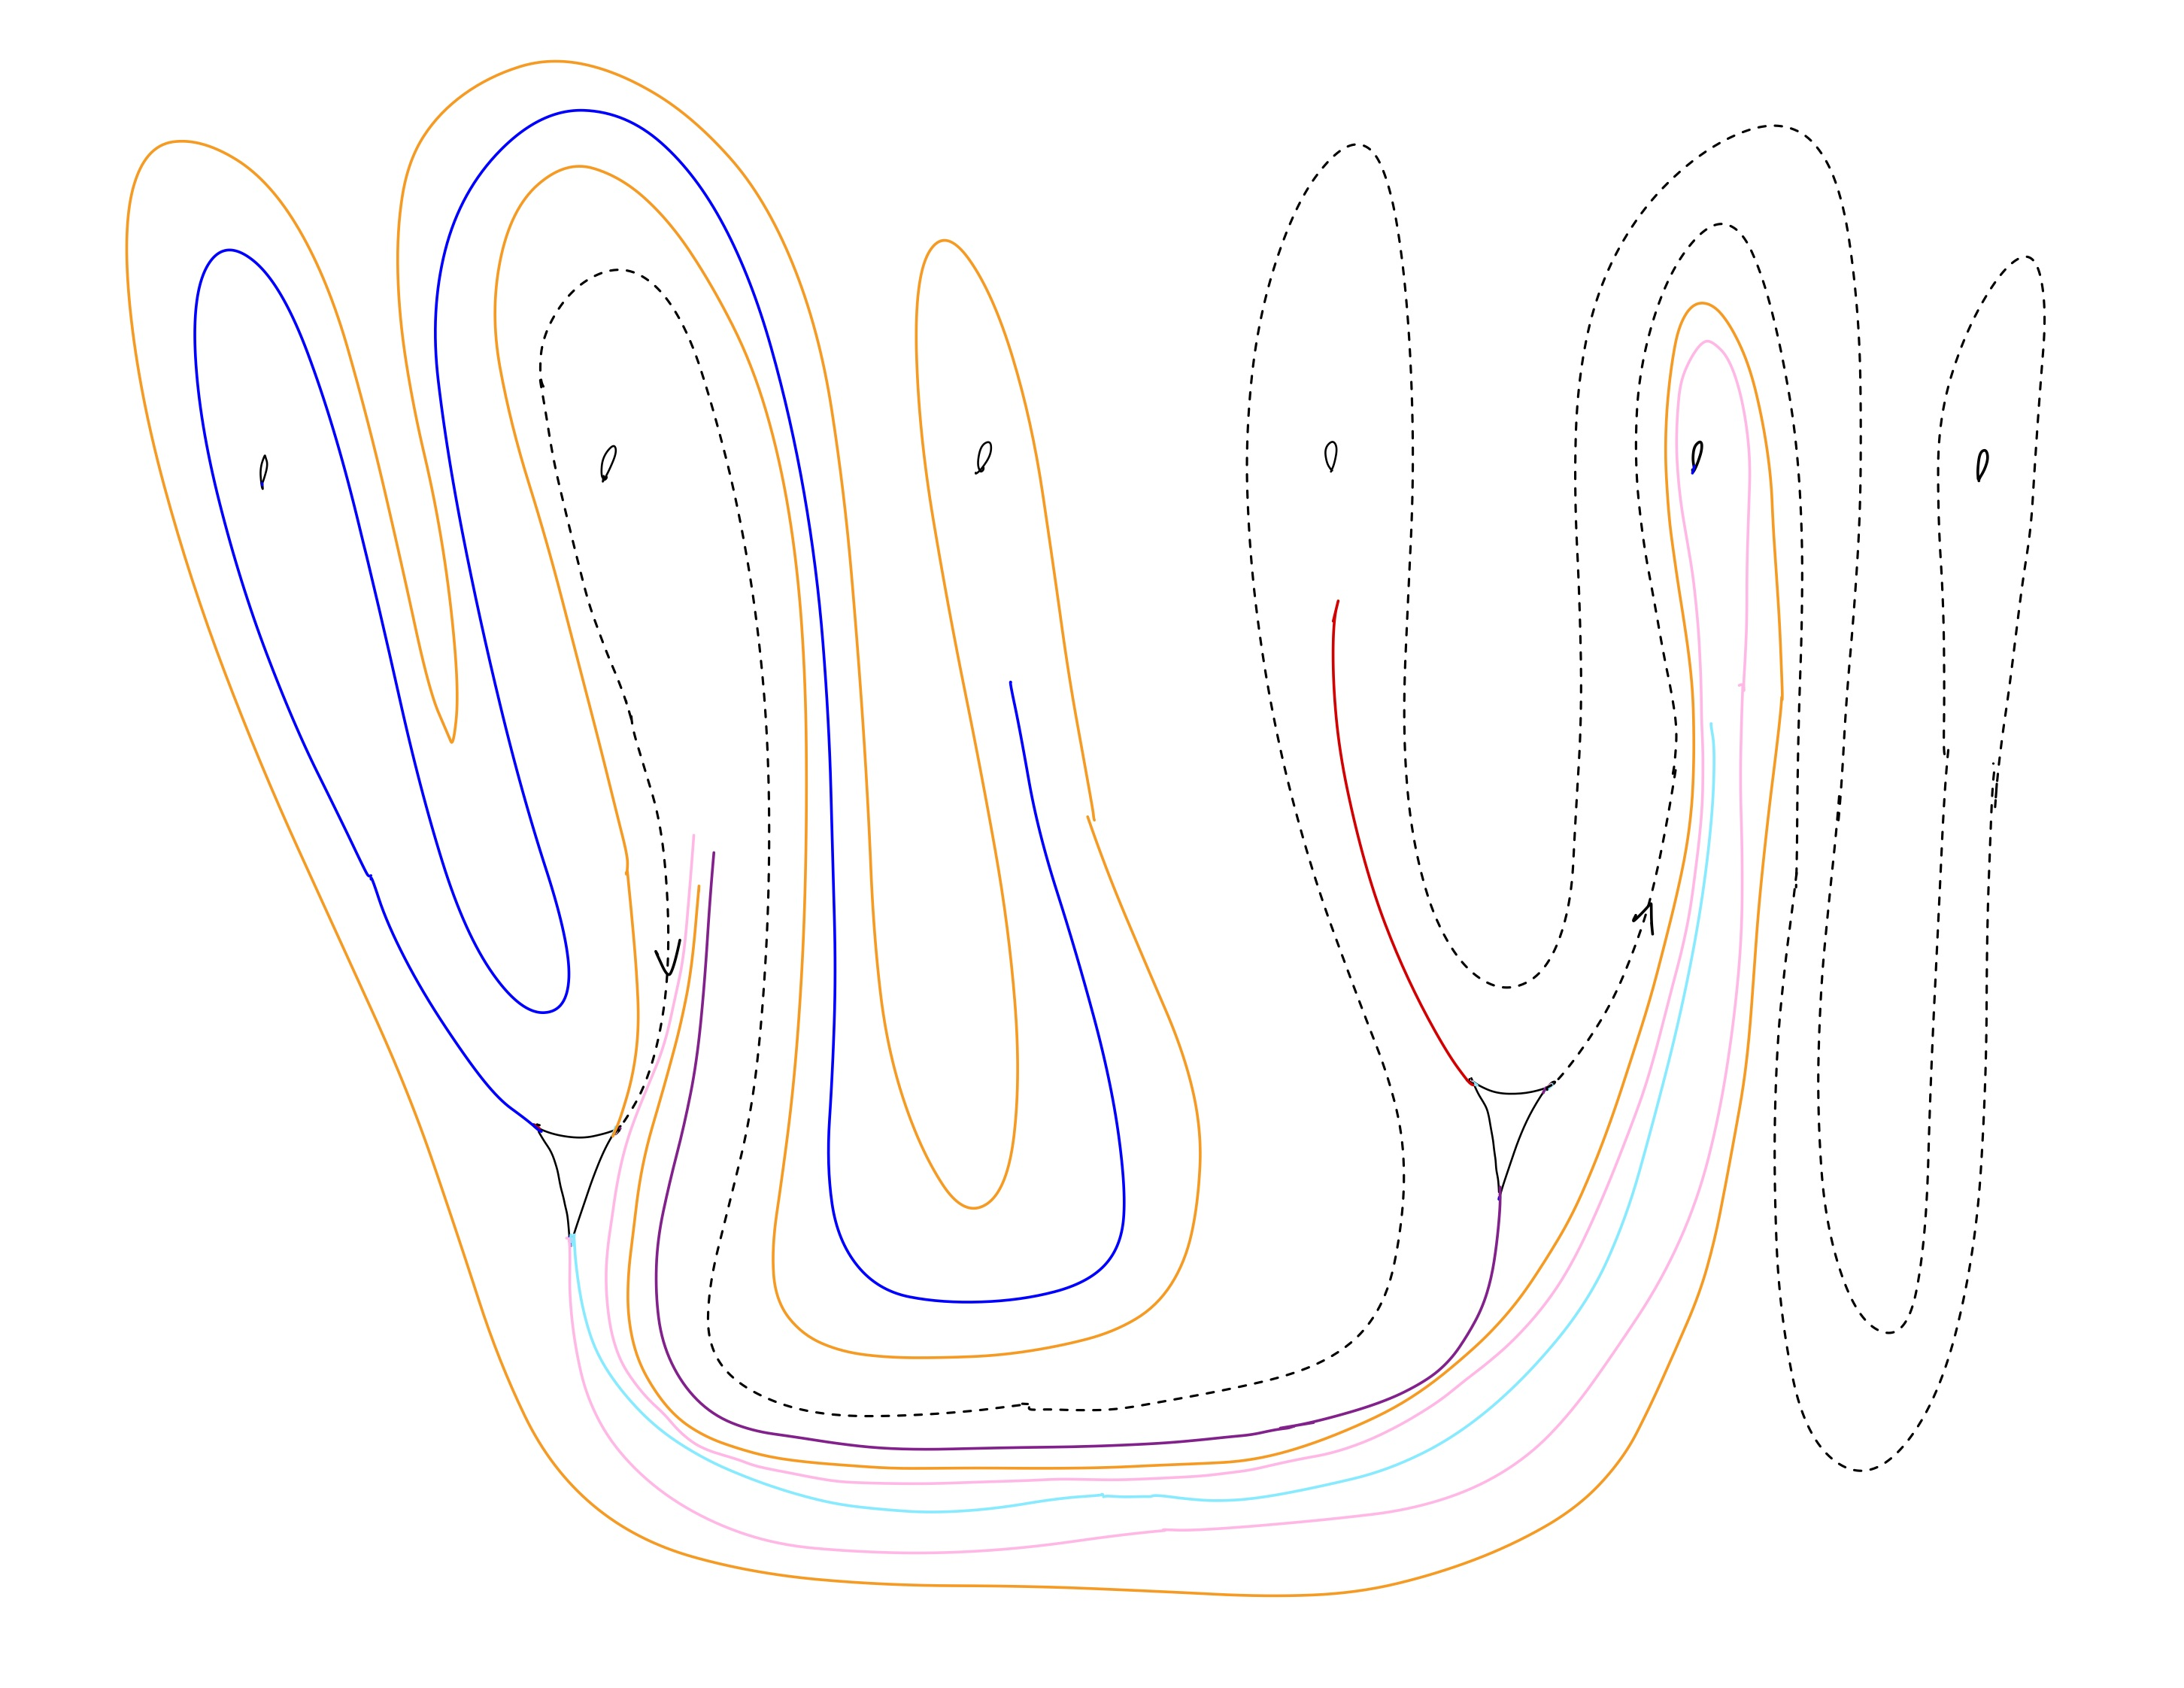
\includegraphics[width=\linewidth]{figures_case_analysis/track17_case_analysis/MMU-13.jpg}
    \caption{MMU13}
    \label{fig:MMU13}
\end{figure}

\begin{figure}[ht]
    \centering
    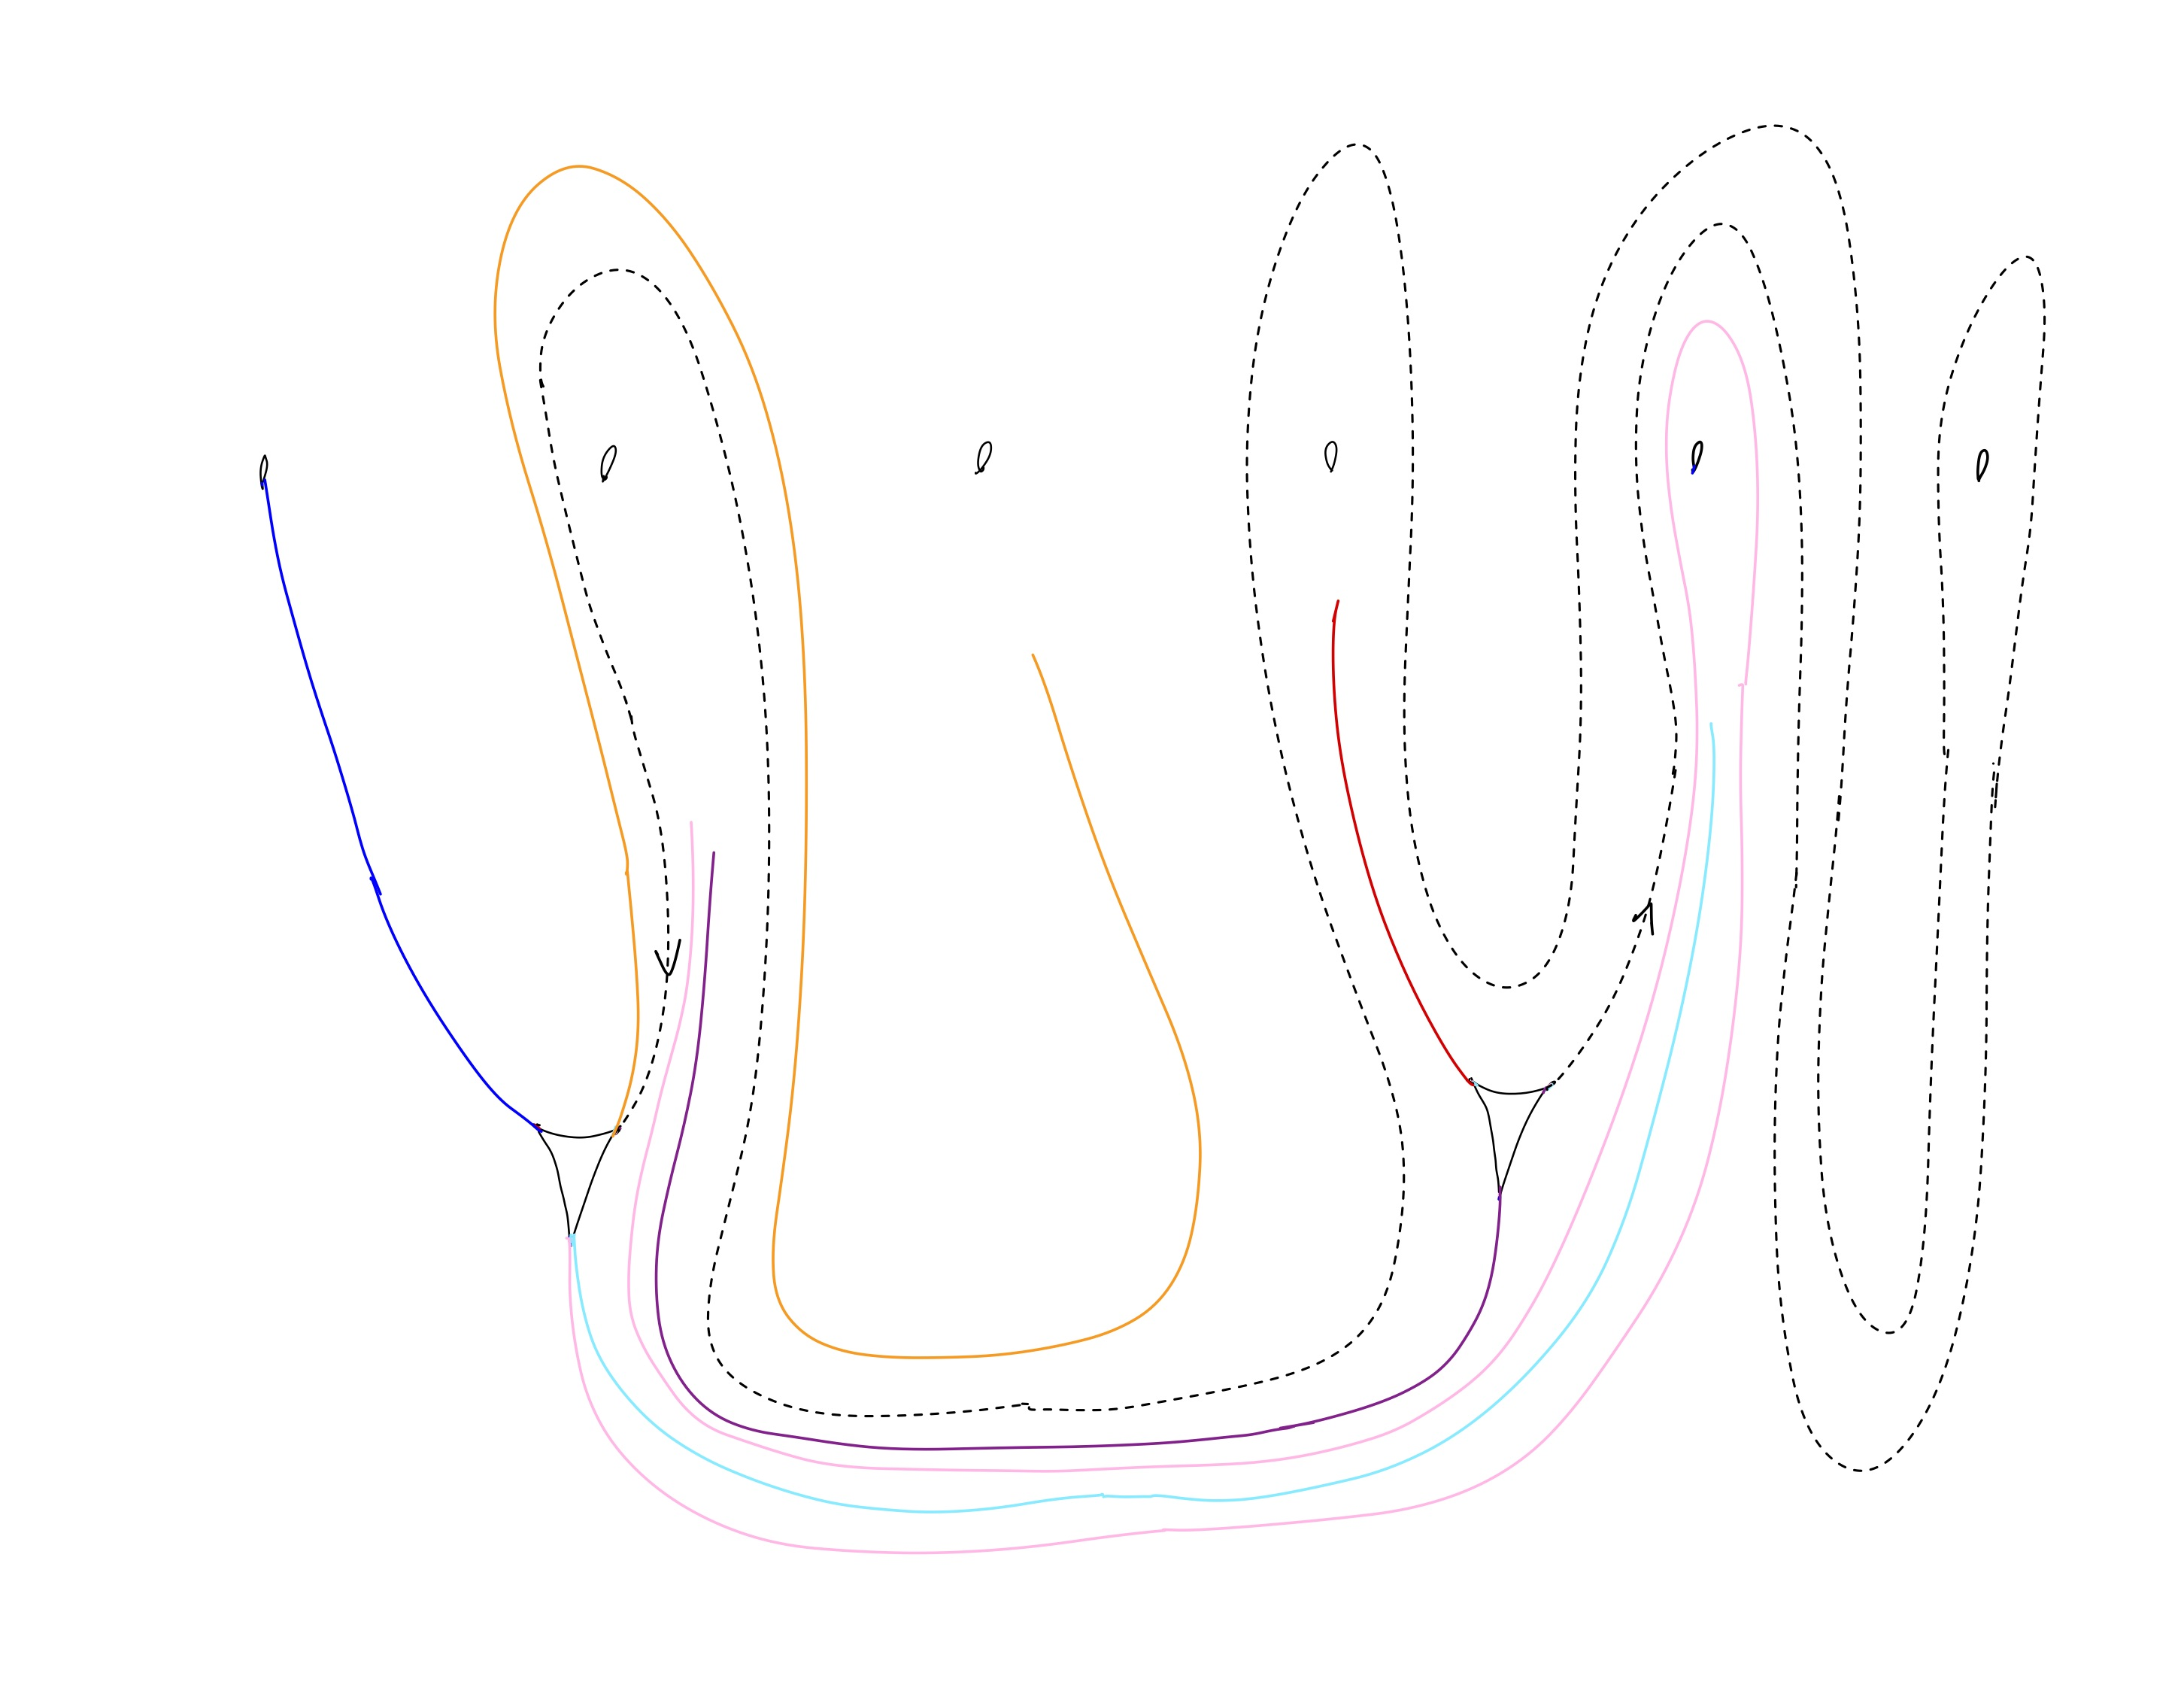
\includegraphics[width=\linewidth]{figures_case_analysis/track17_case_analysis/MMU-14.jpg}
    \caption{MMU14}
    \label{fig:MMU14}
\end{figure}

\begin{figure}[ht]
    \centering
    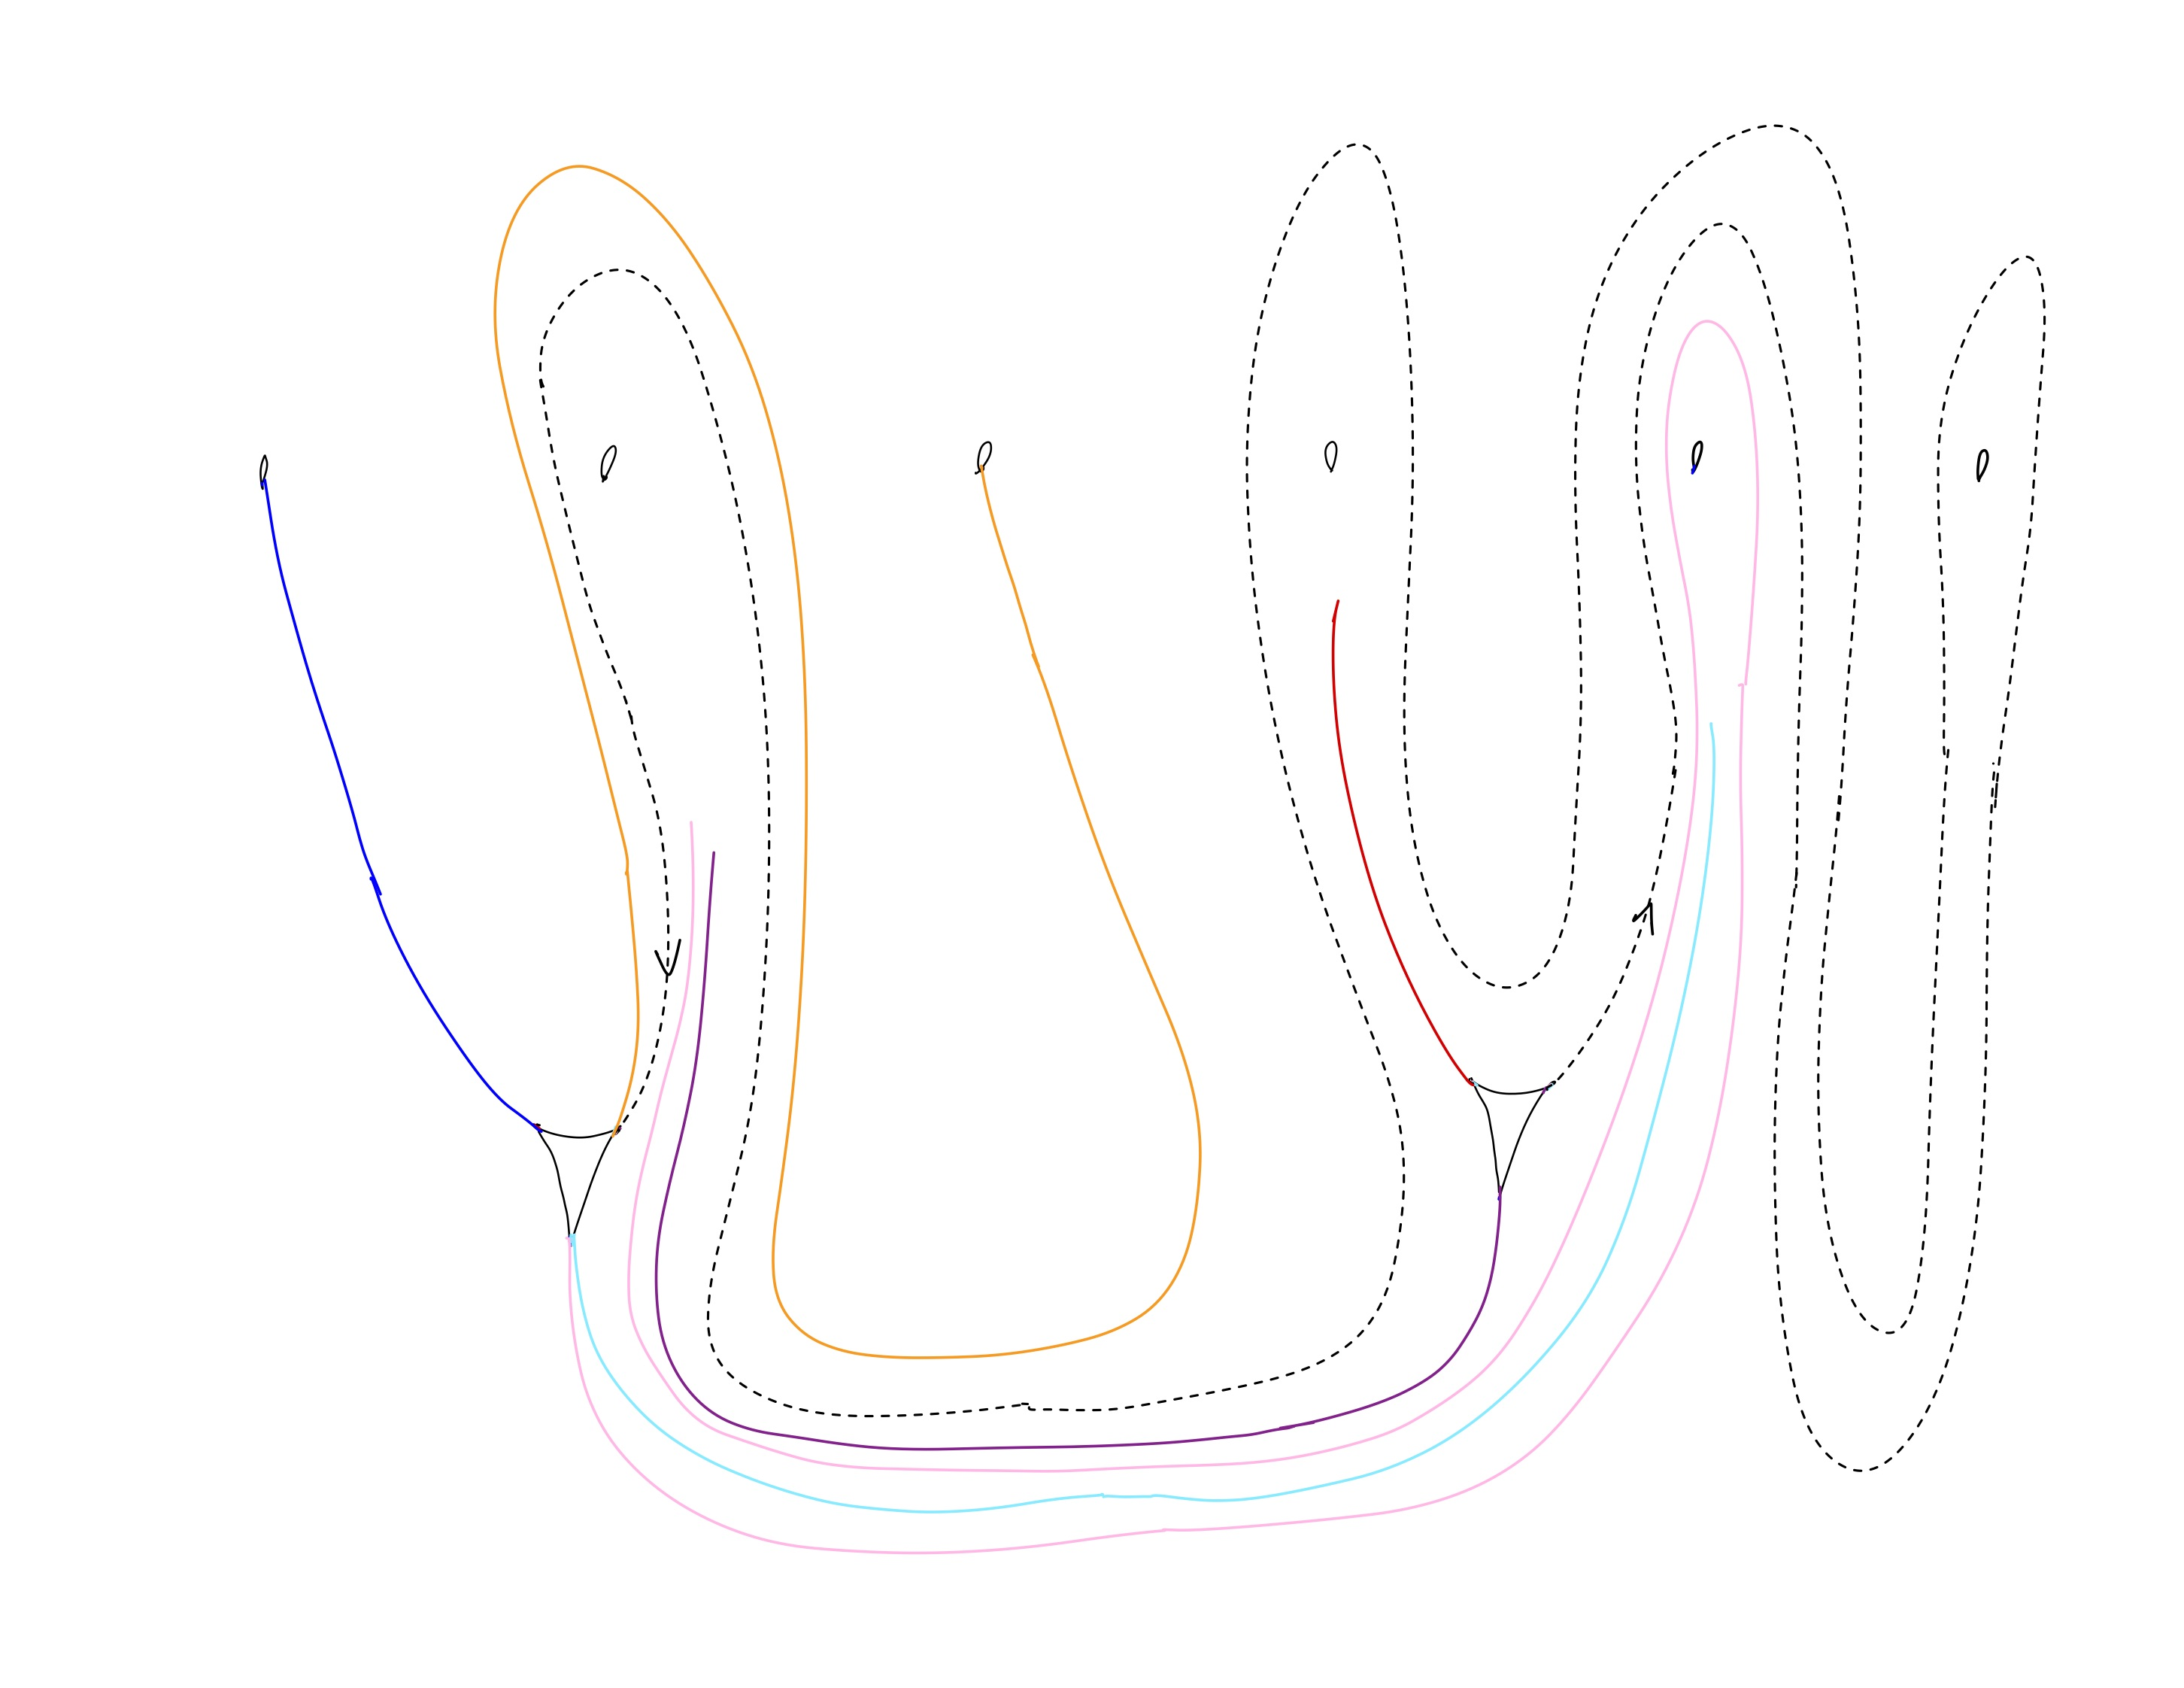
\includegraphics[width=\linewidth]{figures_case_analysis/track17_case_analysis/MMU-15.jpg}
    \caption{MMU15}
    \label{fig:MMU15}
\end{figure}

\begin{figure}[ht]
    \centering
    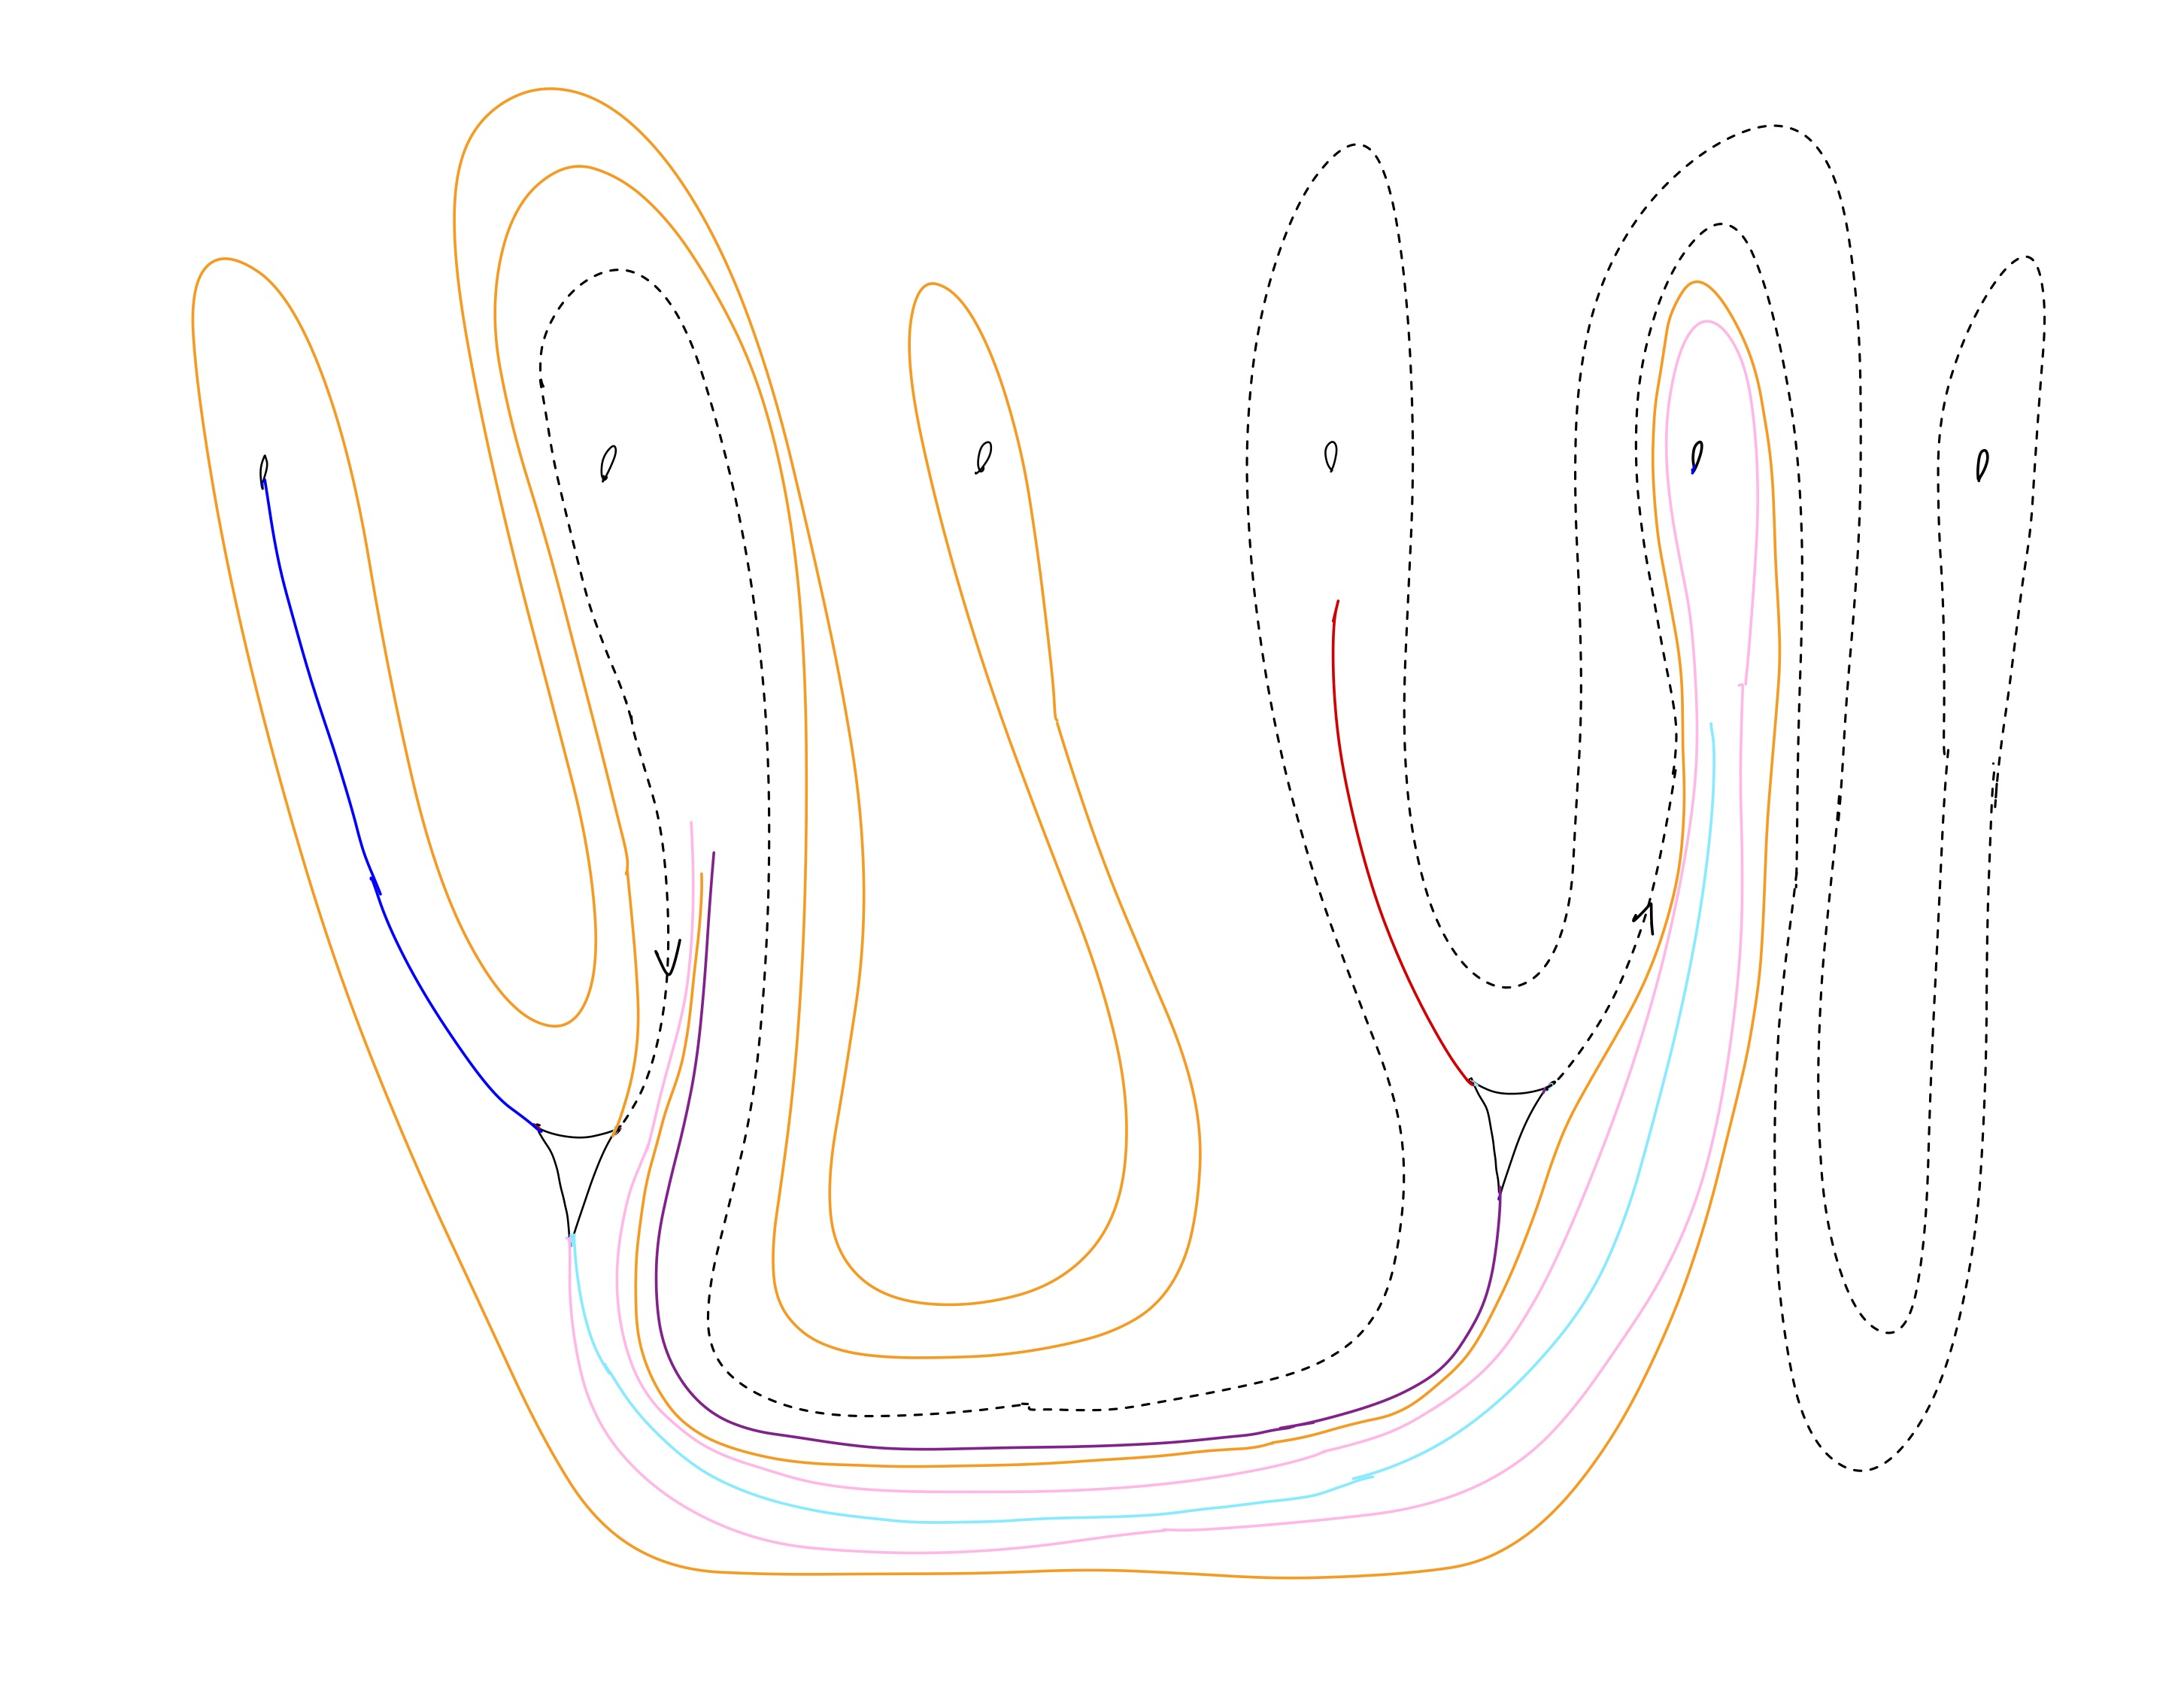
\includegraphics[width=\linewidth]{figures_case_analysis/track17_case_analysis/MMU-16.jpg}
    \caption{MMU16}
    \label{fig:MMU16}
\end{figure}

\begin{figure}[ht]
    \centering
    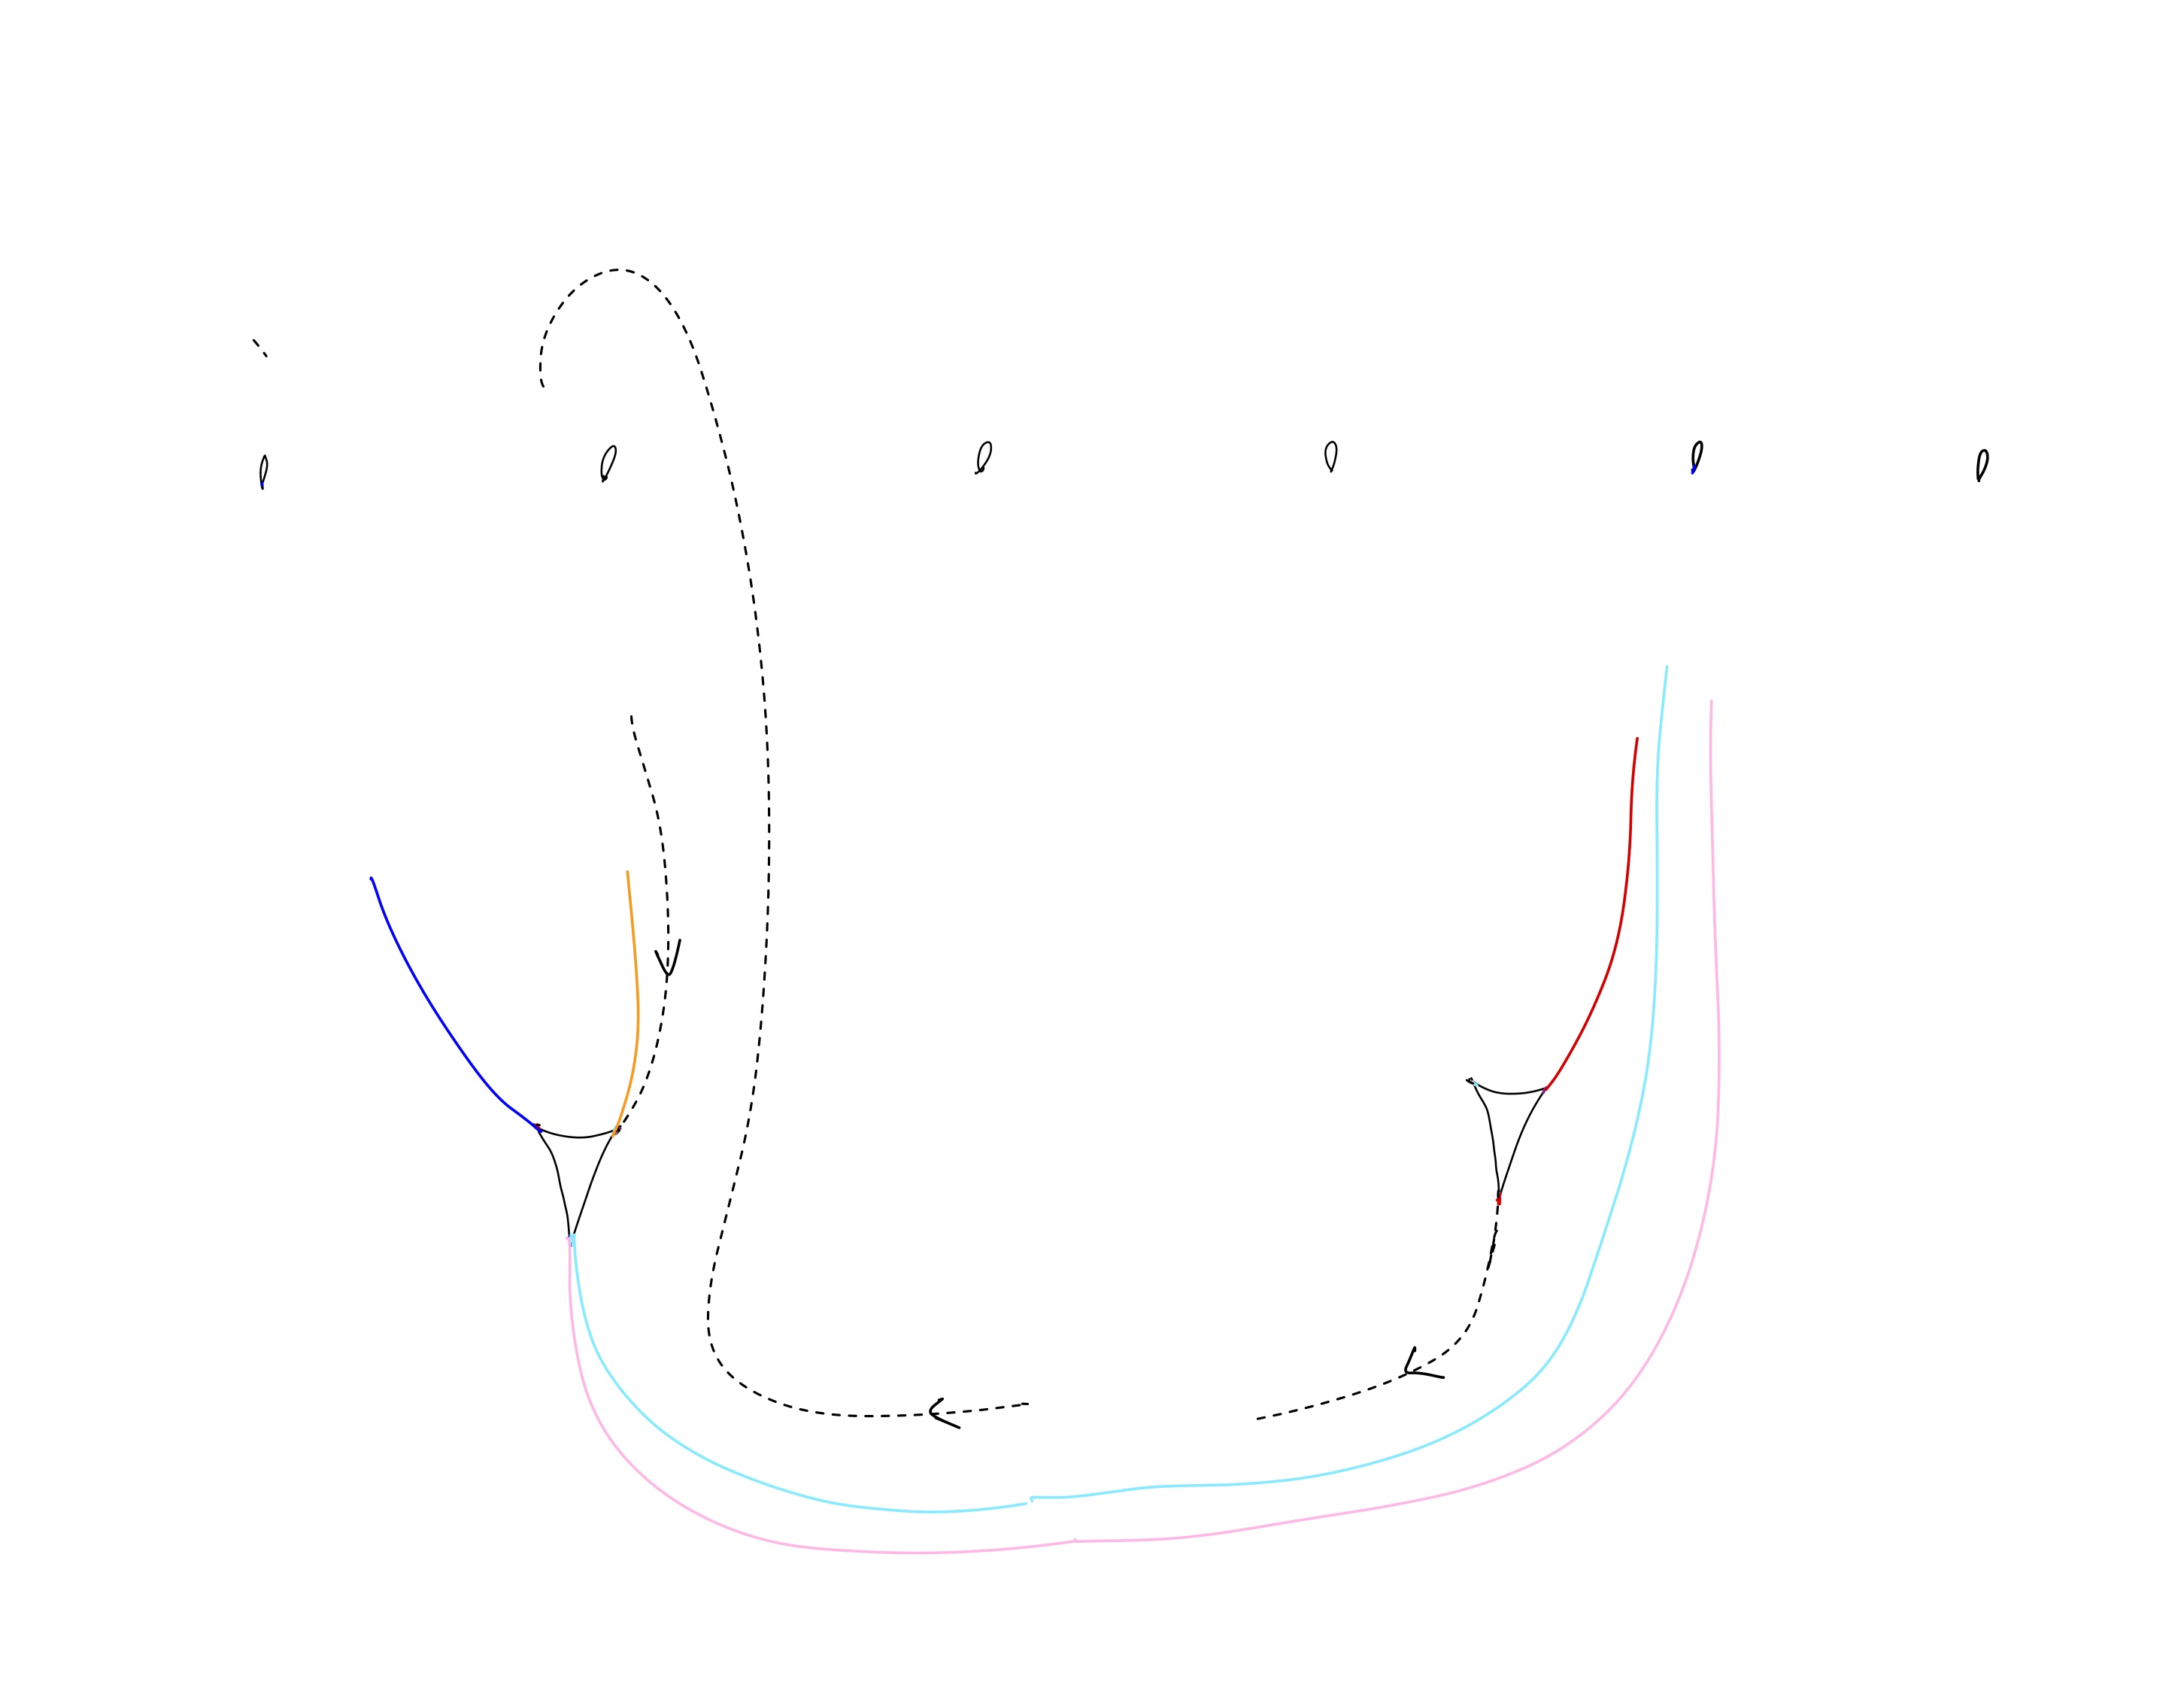
\includegraphics[width=\linewidth]{figures_case_analysis/track17_case_analysis/MMU-17.jpg}
    \caption{MMU17}
    \label{fig:MMU17}
\end{figure}

\begin{figure}[ht]
    \centering
    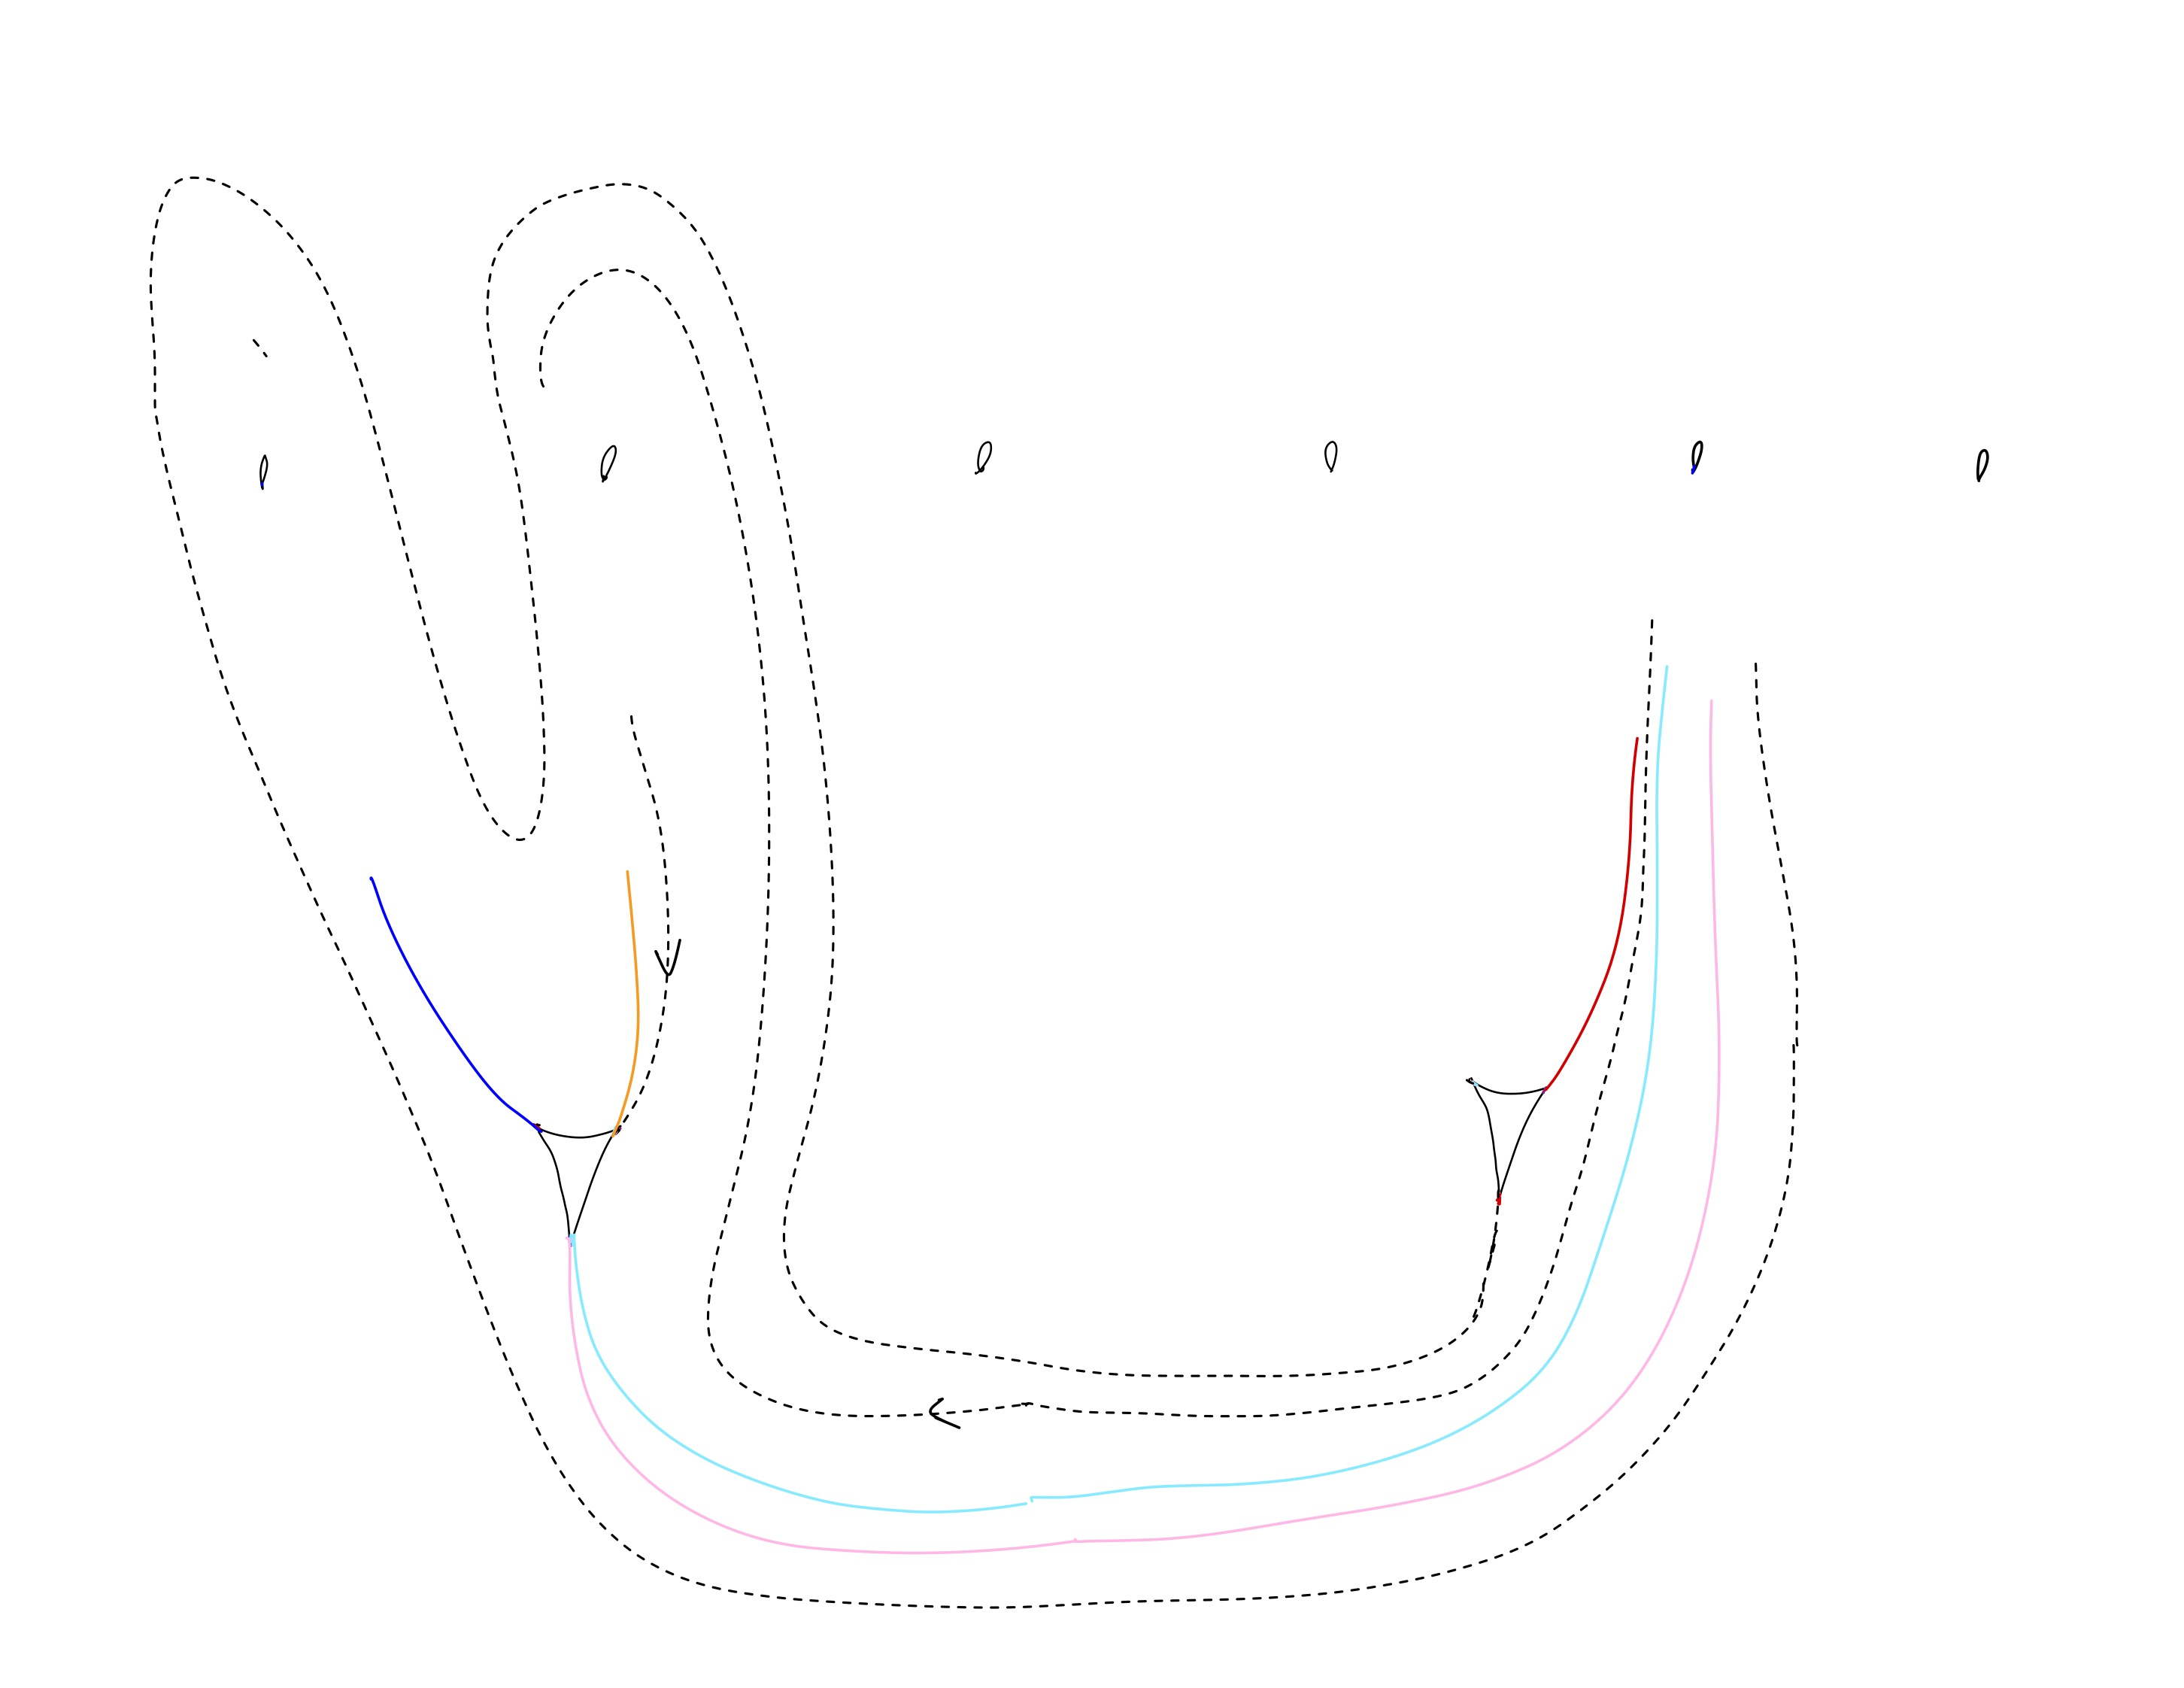
\includegraphics[width=\linewidth]{figures_case_analysis/track17_case_analysis/MMU-18.jpg}
    \caption{MMU18}
    \label{fig:MMU18}
\end{figure}

\begin{figure}[ht]
    \centering
    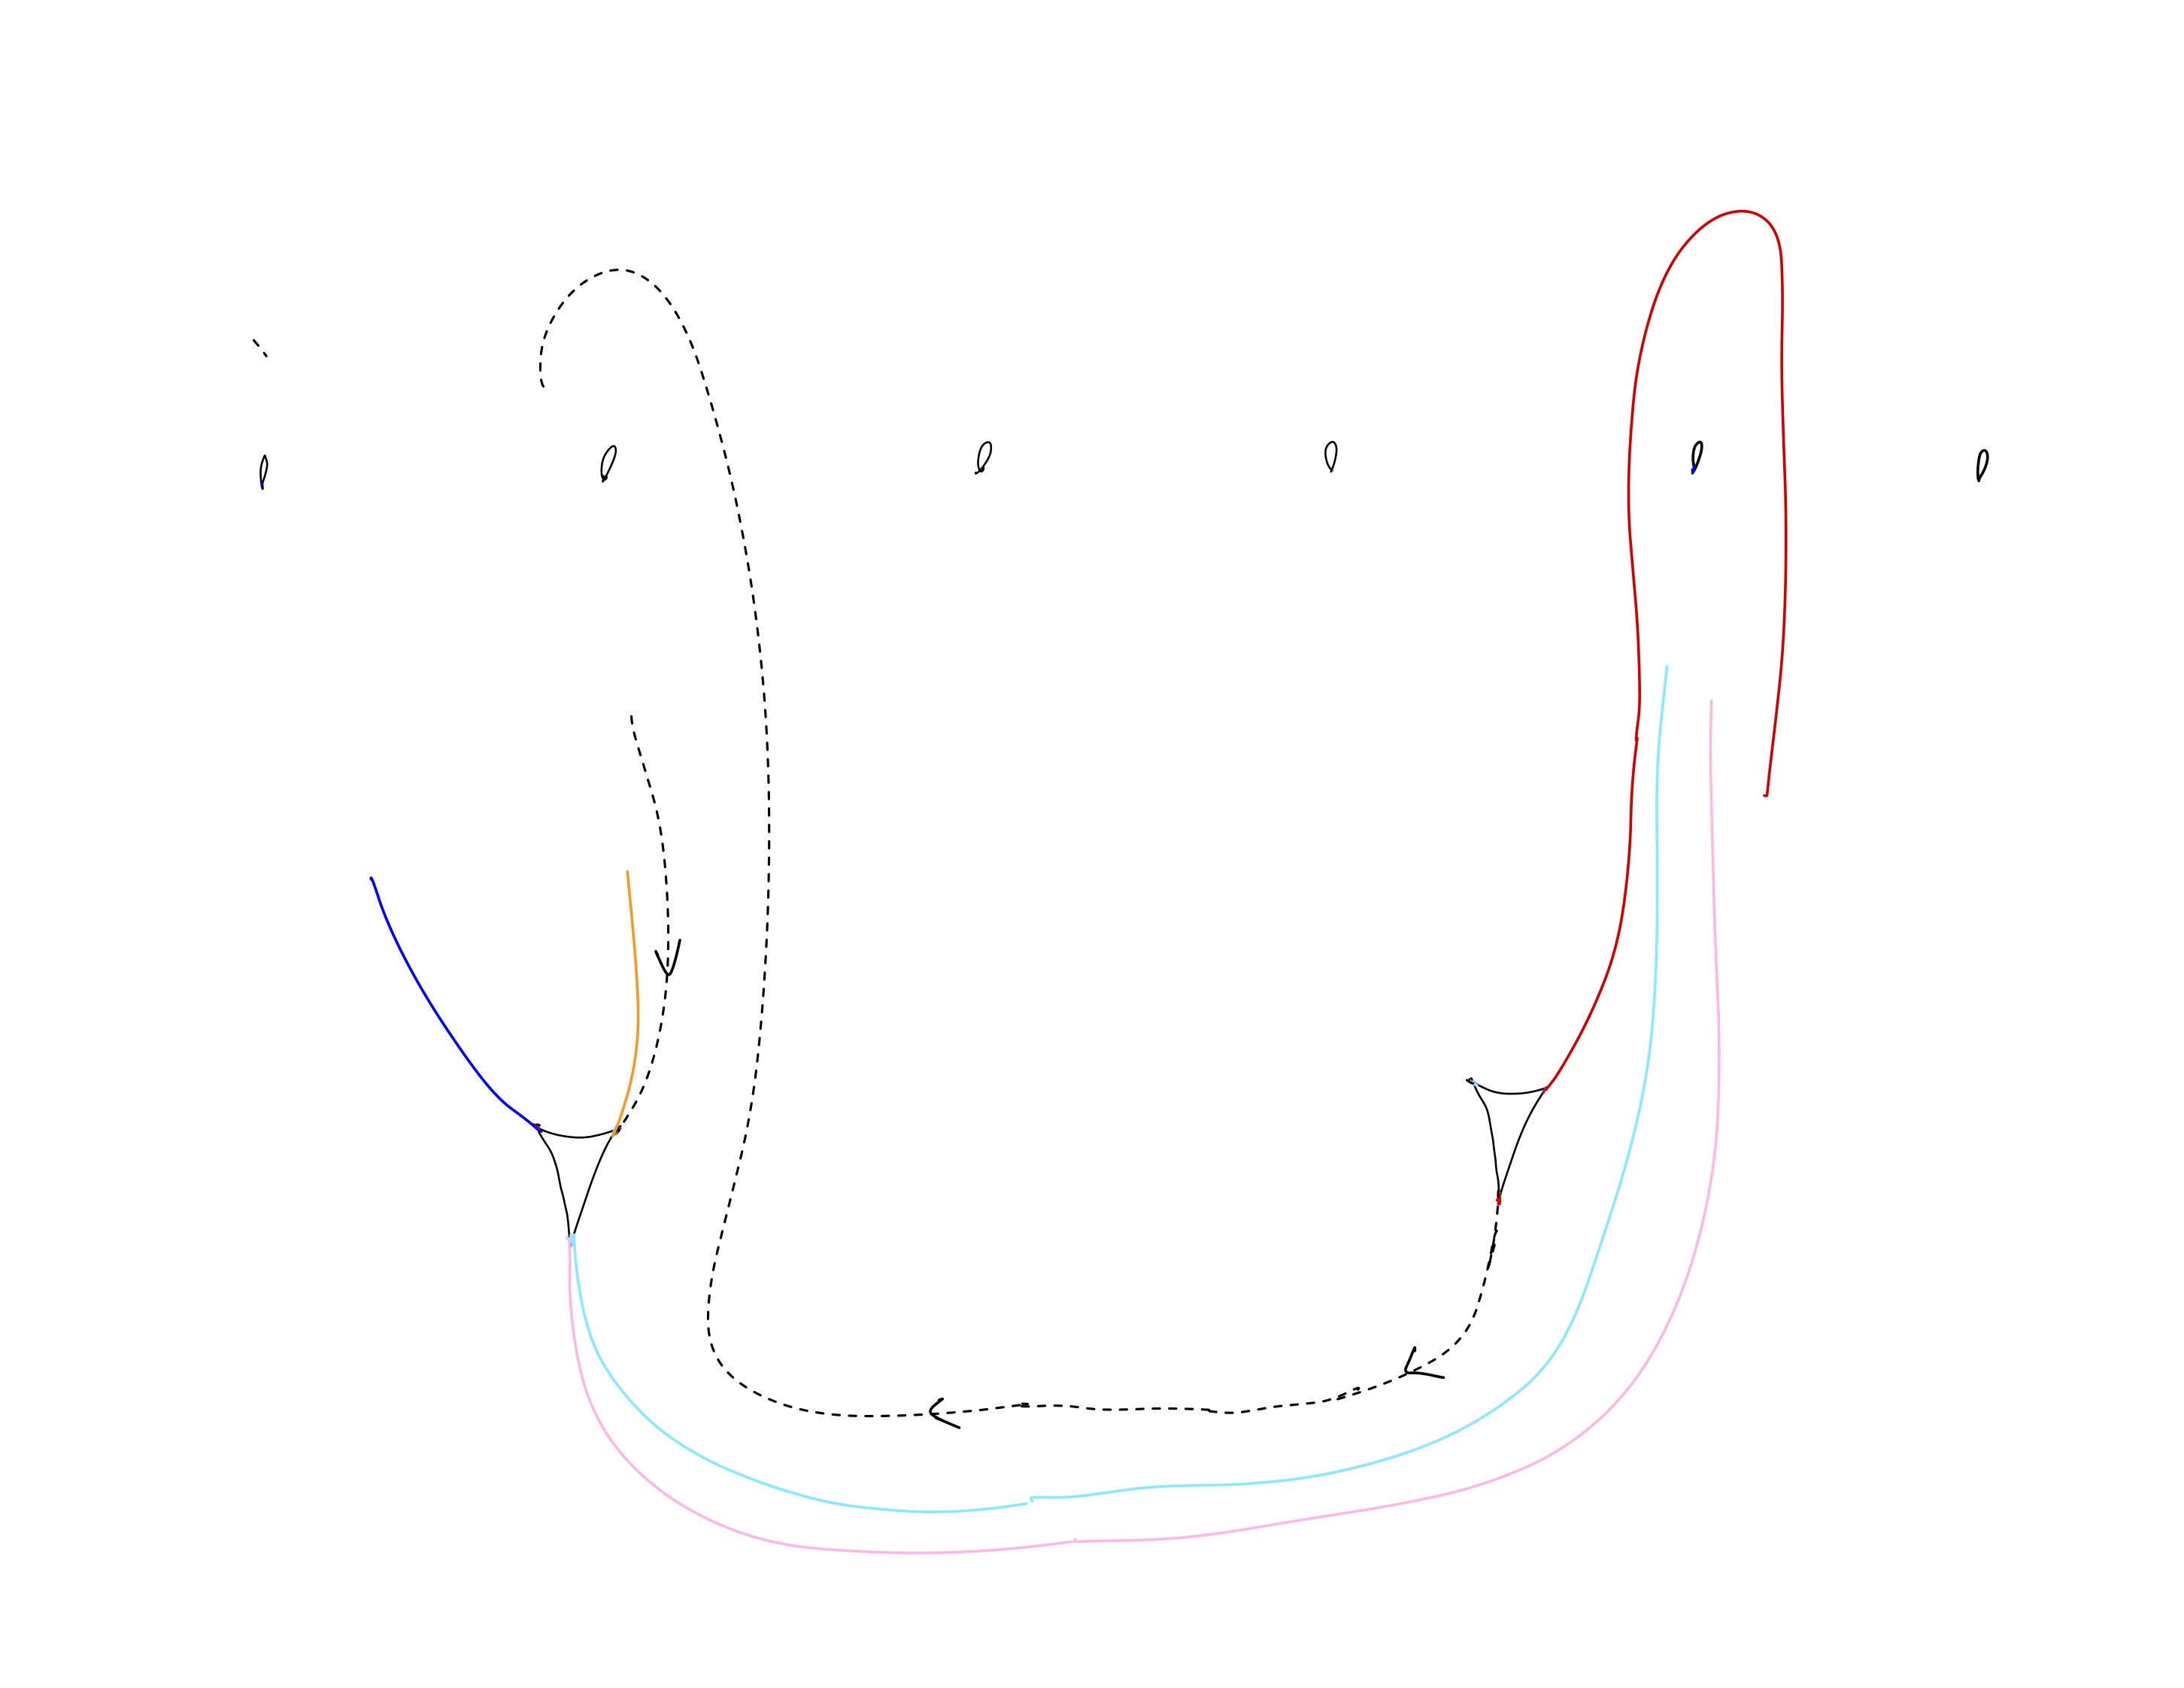
\includegraphics[width=\linewidth]{figures_case_analysis/track17_case_analysis/MMU-19.jpg}
    \caption{MMU19}
    \label{fig:MMU19}
\end{figure}

\begin{figure}[ht]
    \centering
    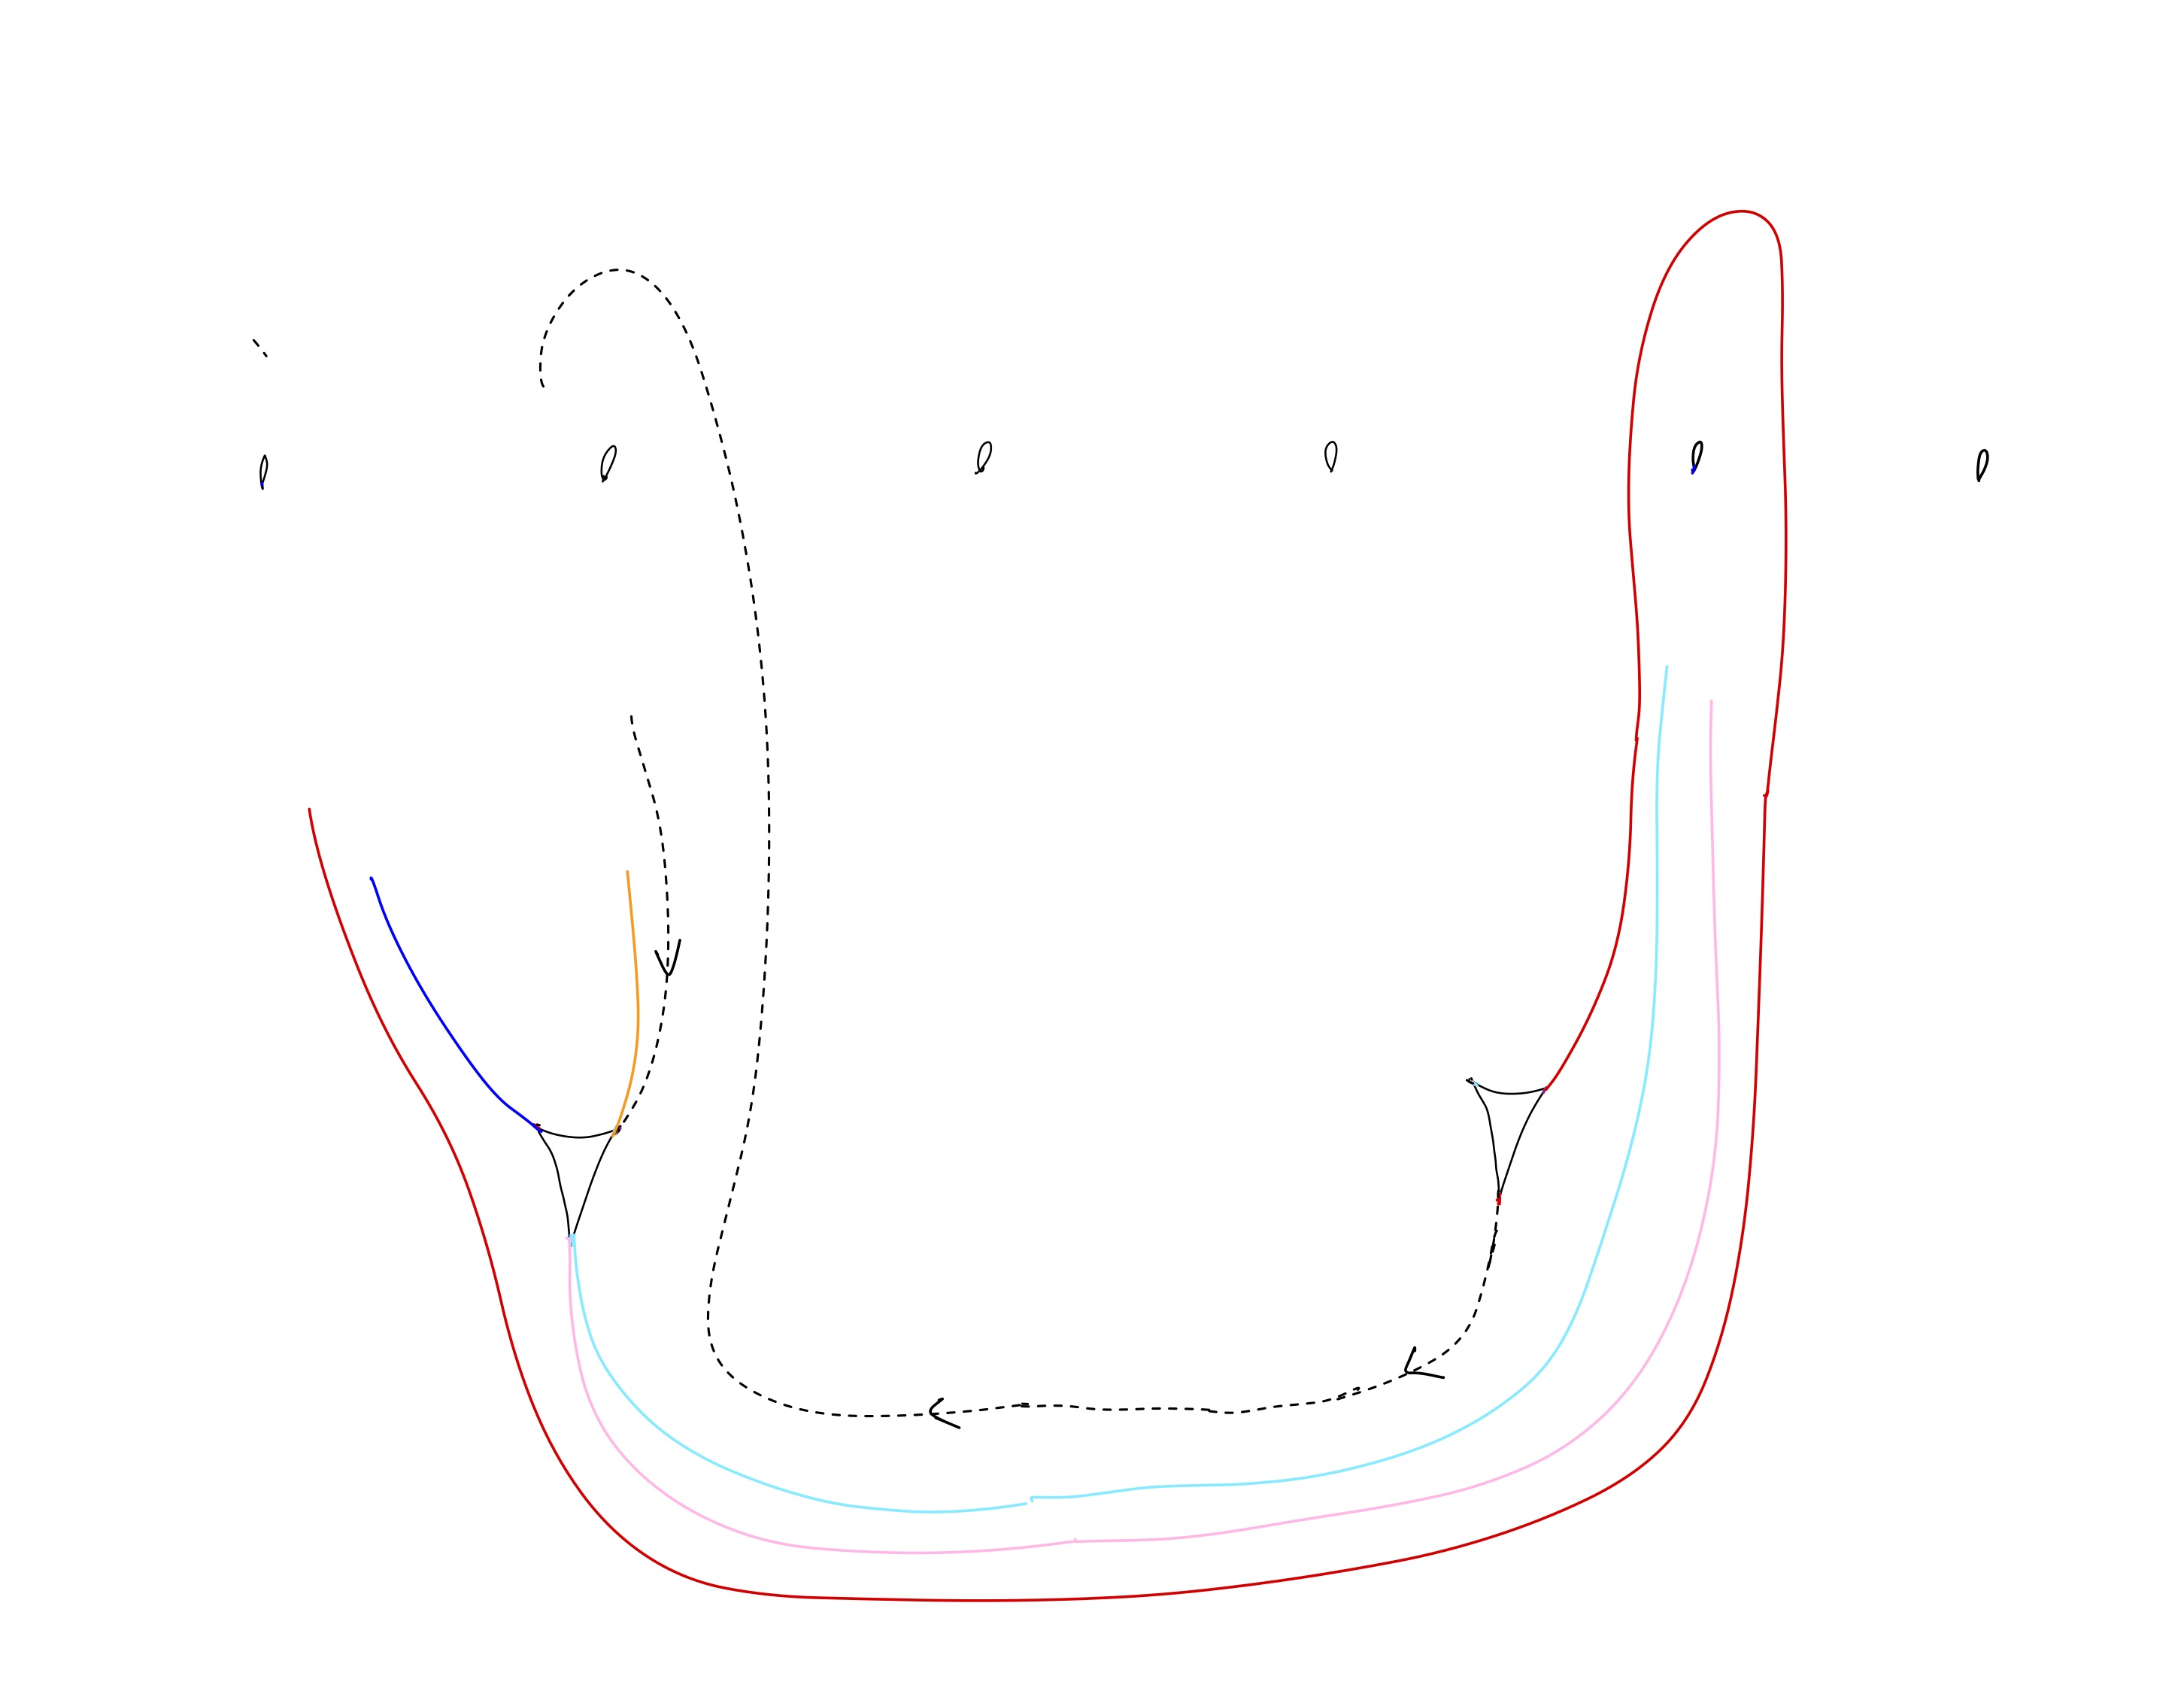
\includegraphics[width=\linewidth]{figures_case_analysis/track17_case_analysis/MMU-20.jpg}
    \caption{MMU20}
    \label{fig:MMU20}
\end{figure}

\begin{figure}[ht]
    \centering
    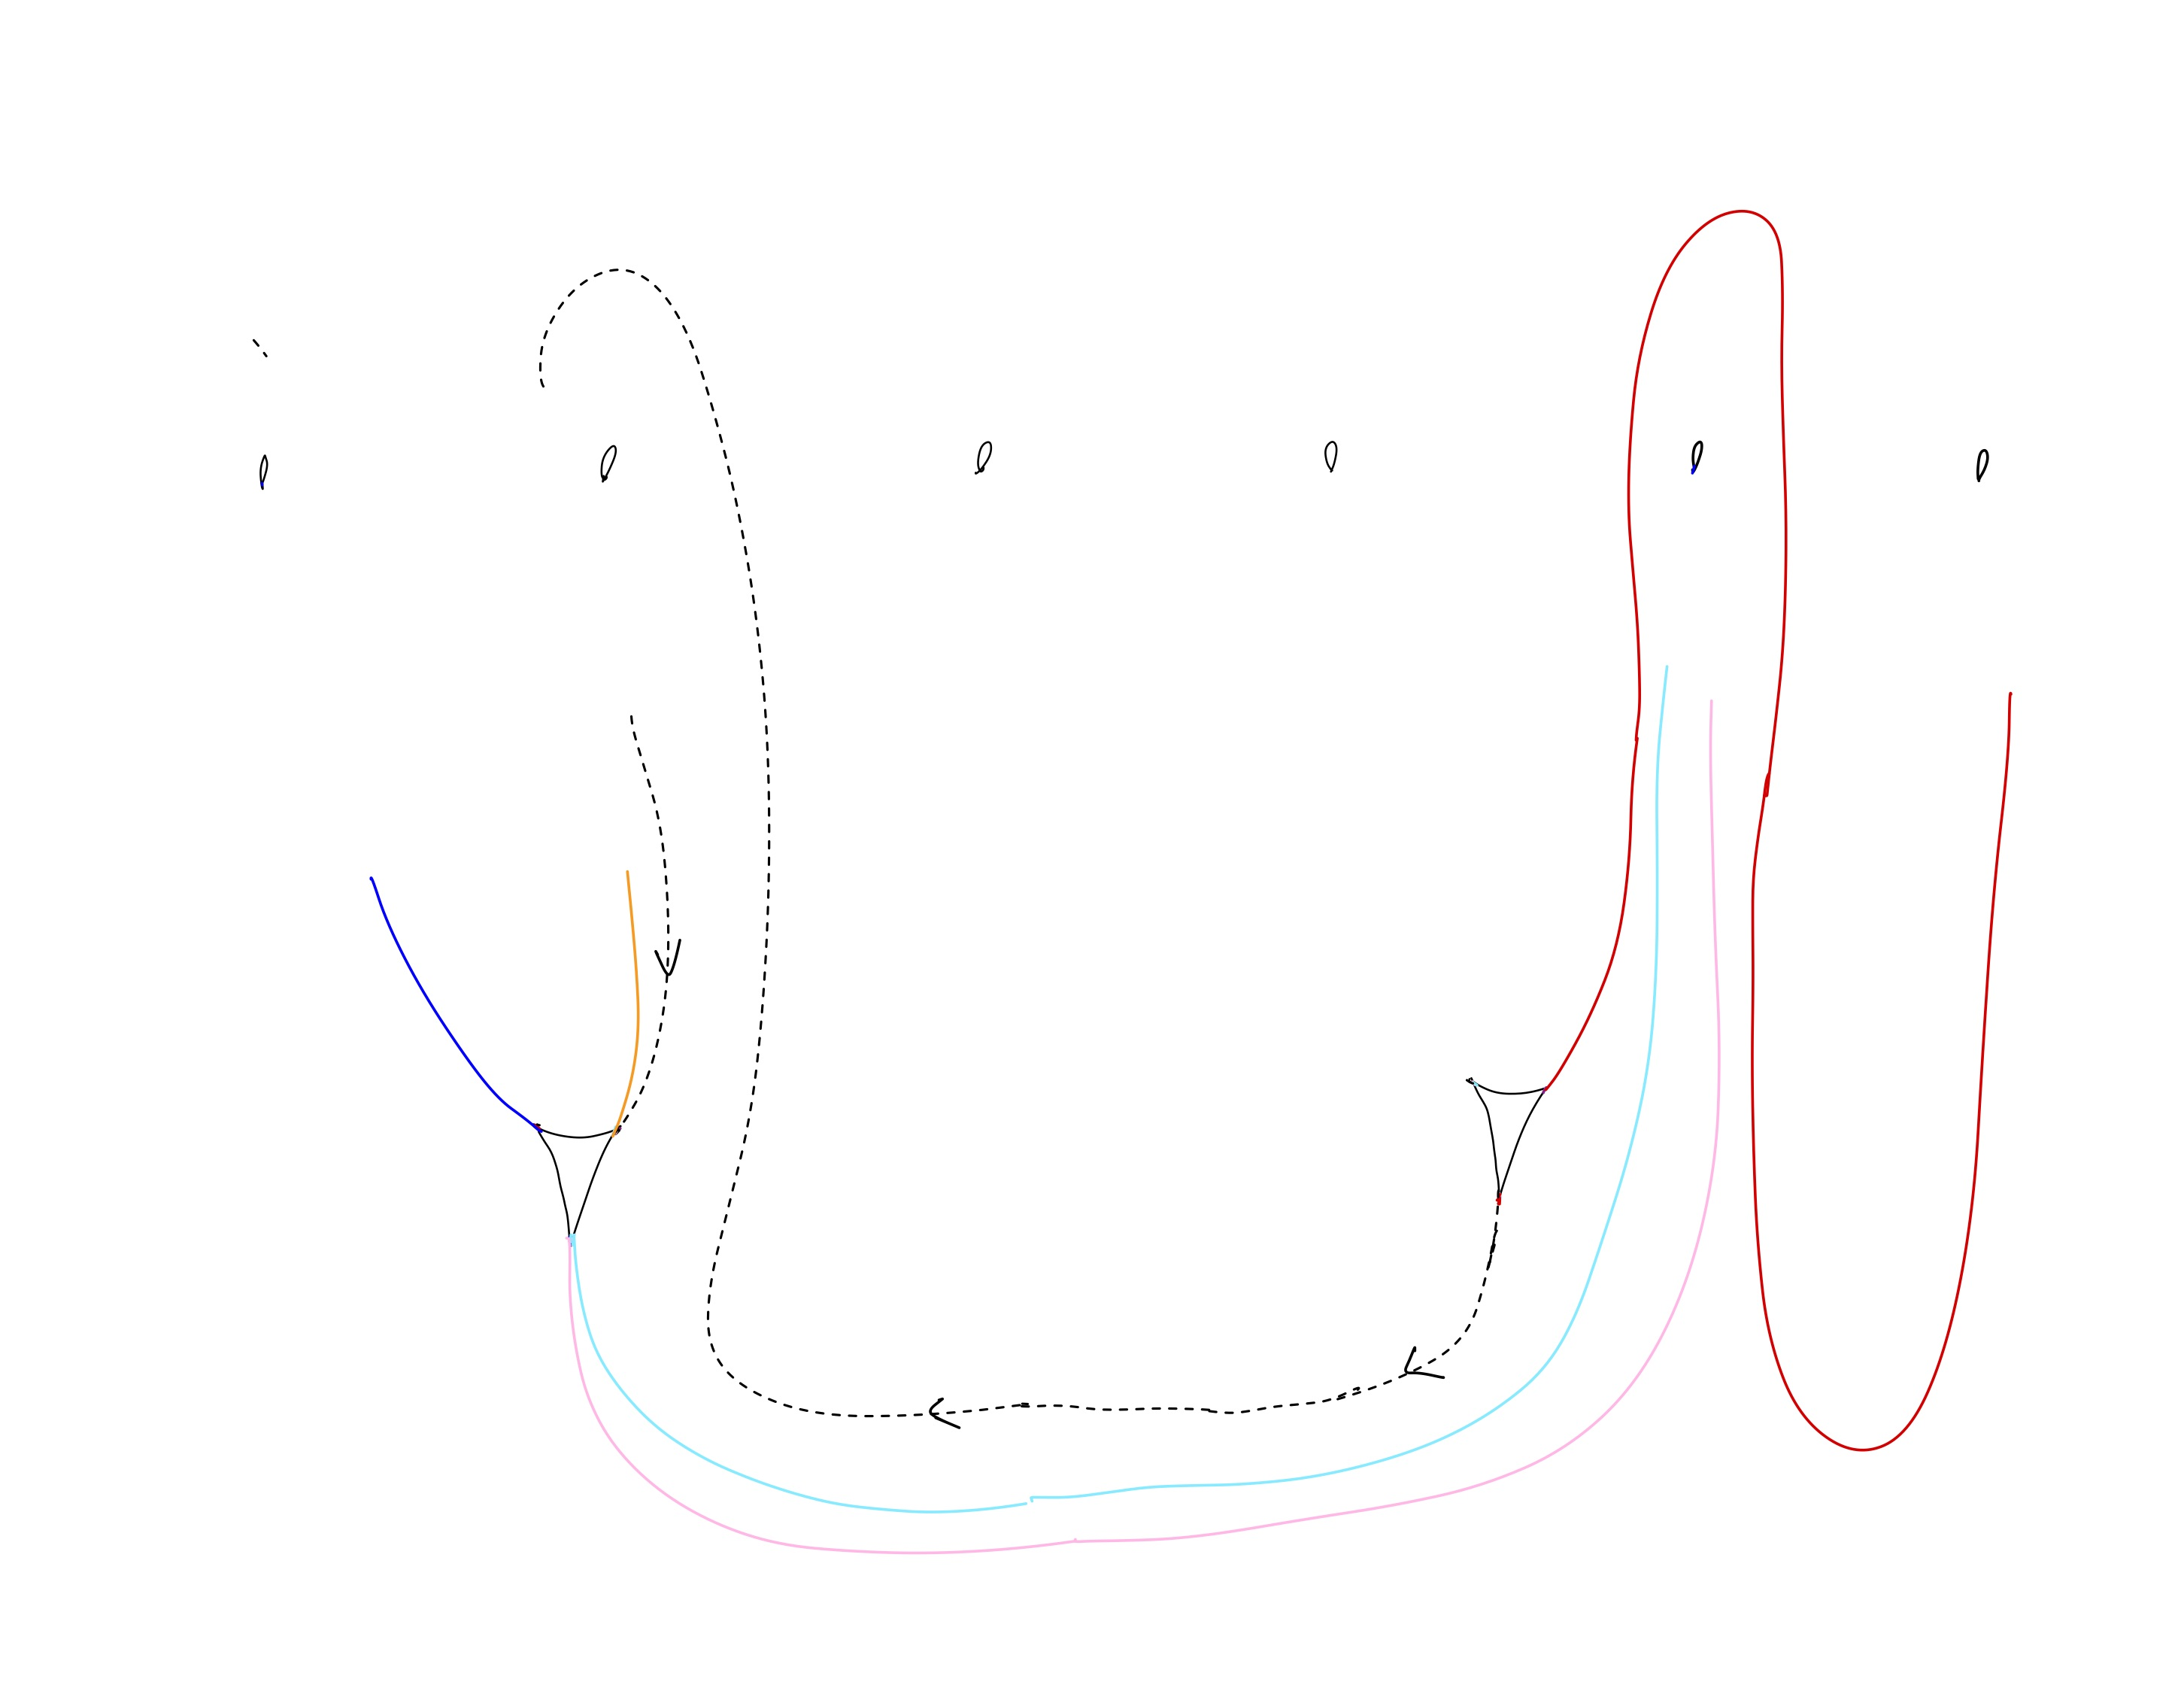
\includegraphics[width=\linewidth]{figures_case_analysis/track17_case_analysis/MMU-21.jpg}
    \caption{MMU21}
    \label{fig:MMU21}
\end{figure}

\begin{figure}[ht]
    \centering
    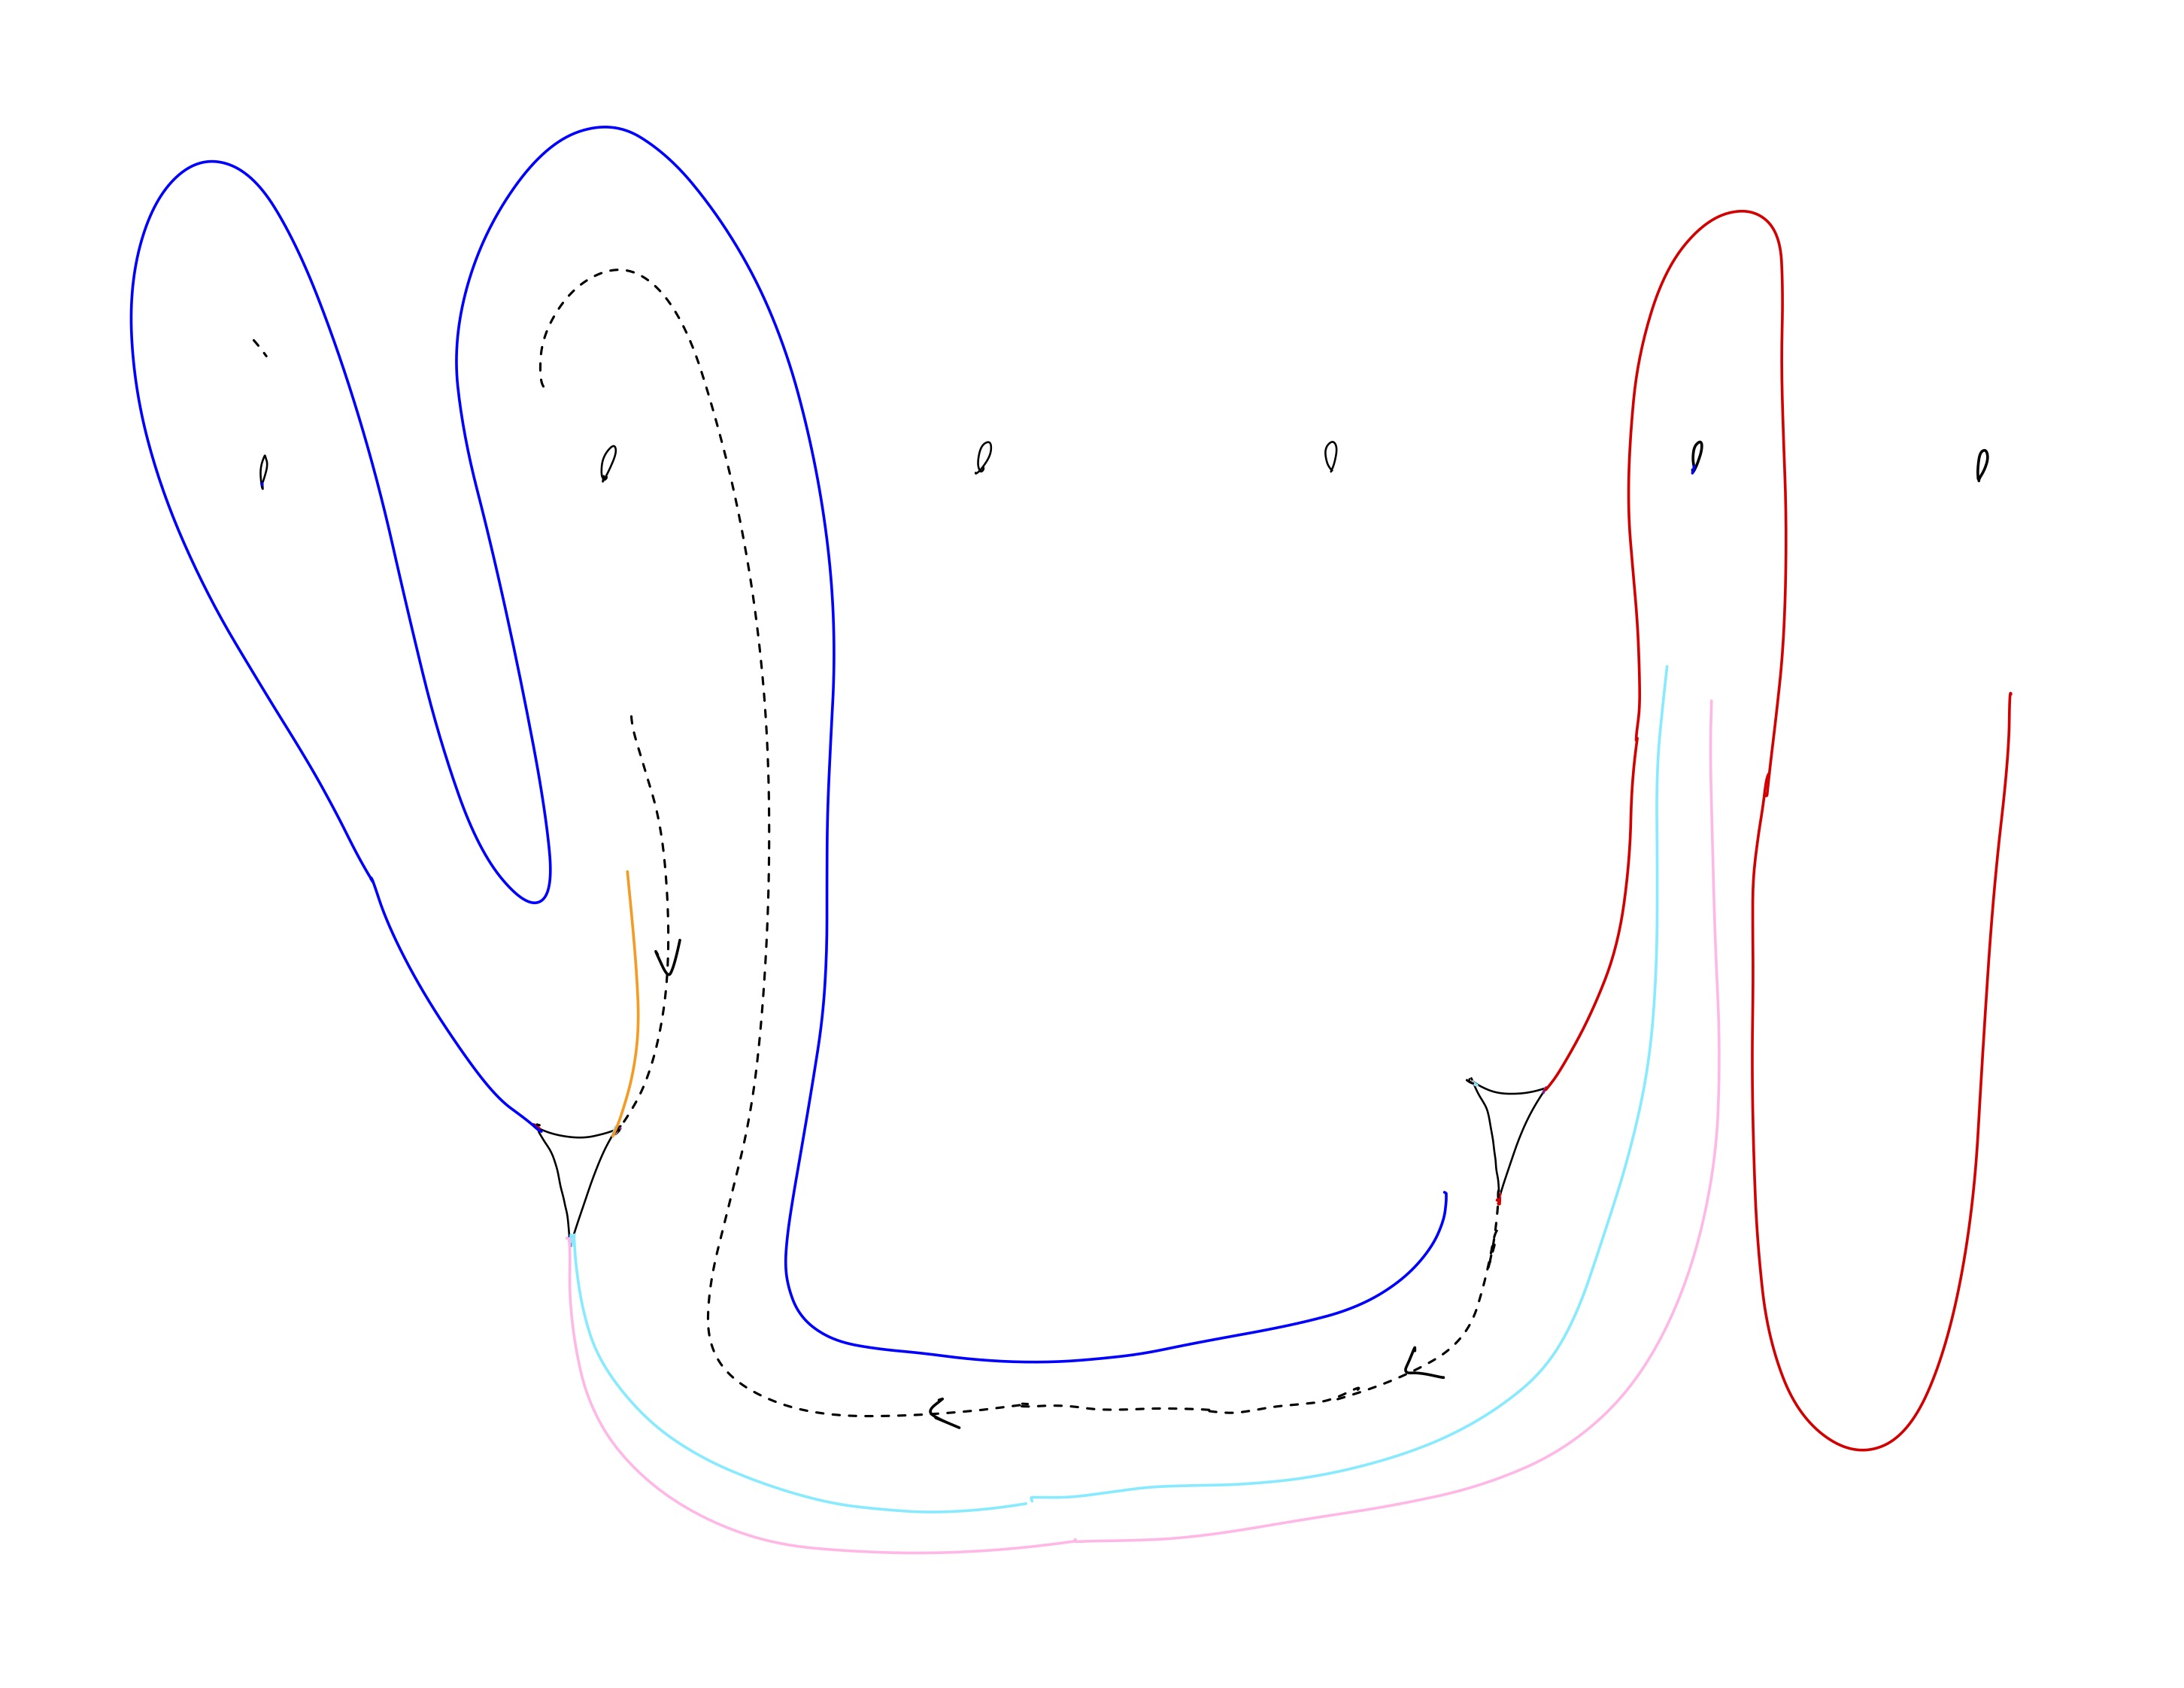
\includegraphics[width=\linewidth]{figures_case_analysis/track17_case_analysis/MMU-22.jpg}
    \caption{MMU22}
    \label{fig:MMU22}
\end{figure}

\begin{figure}[ht]
    \centering
    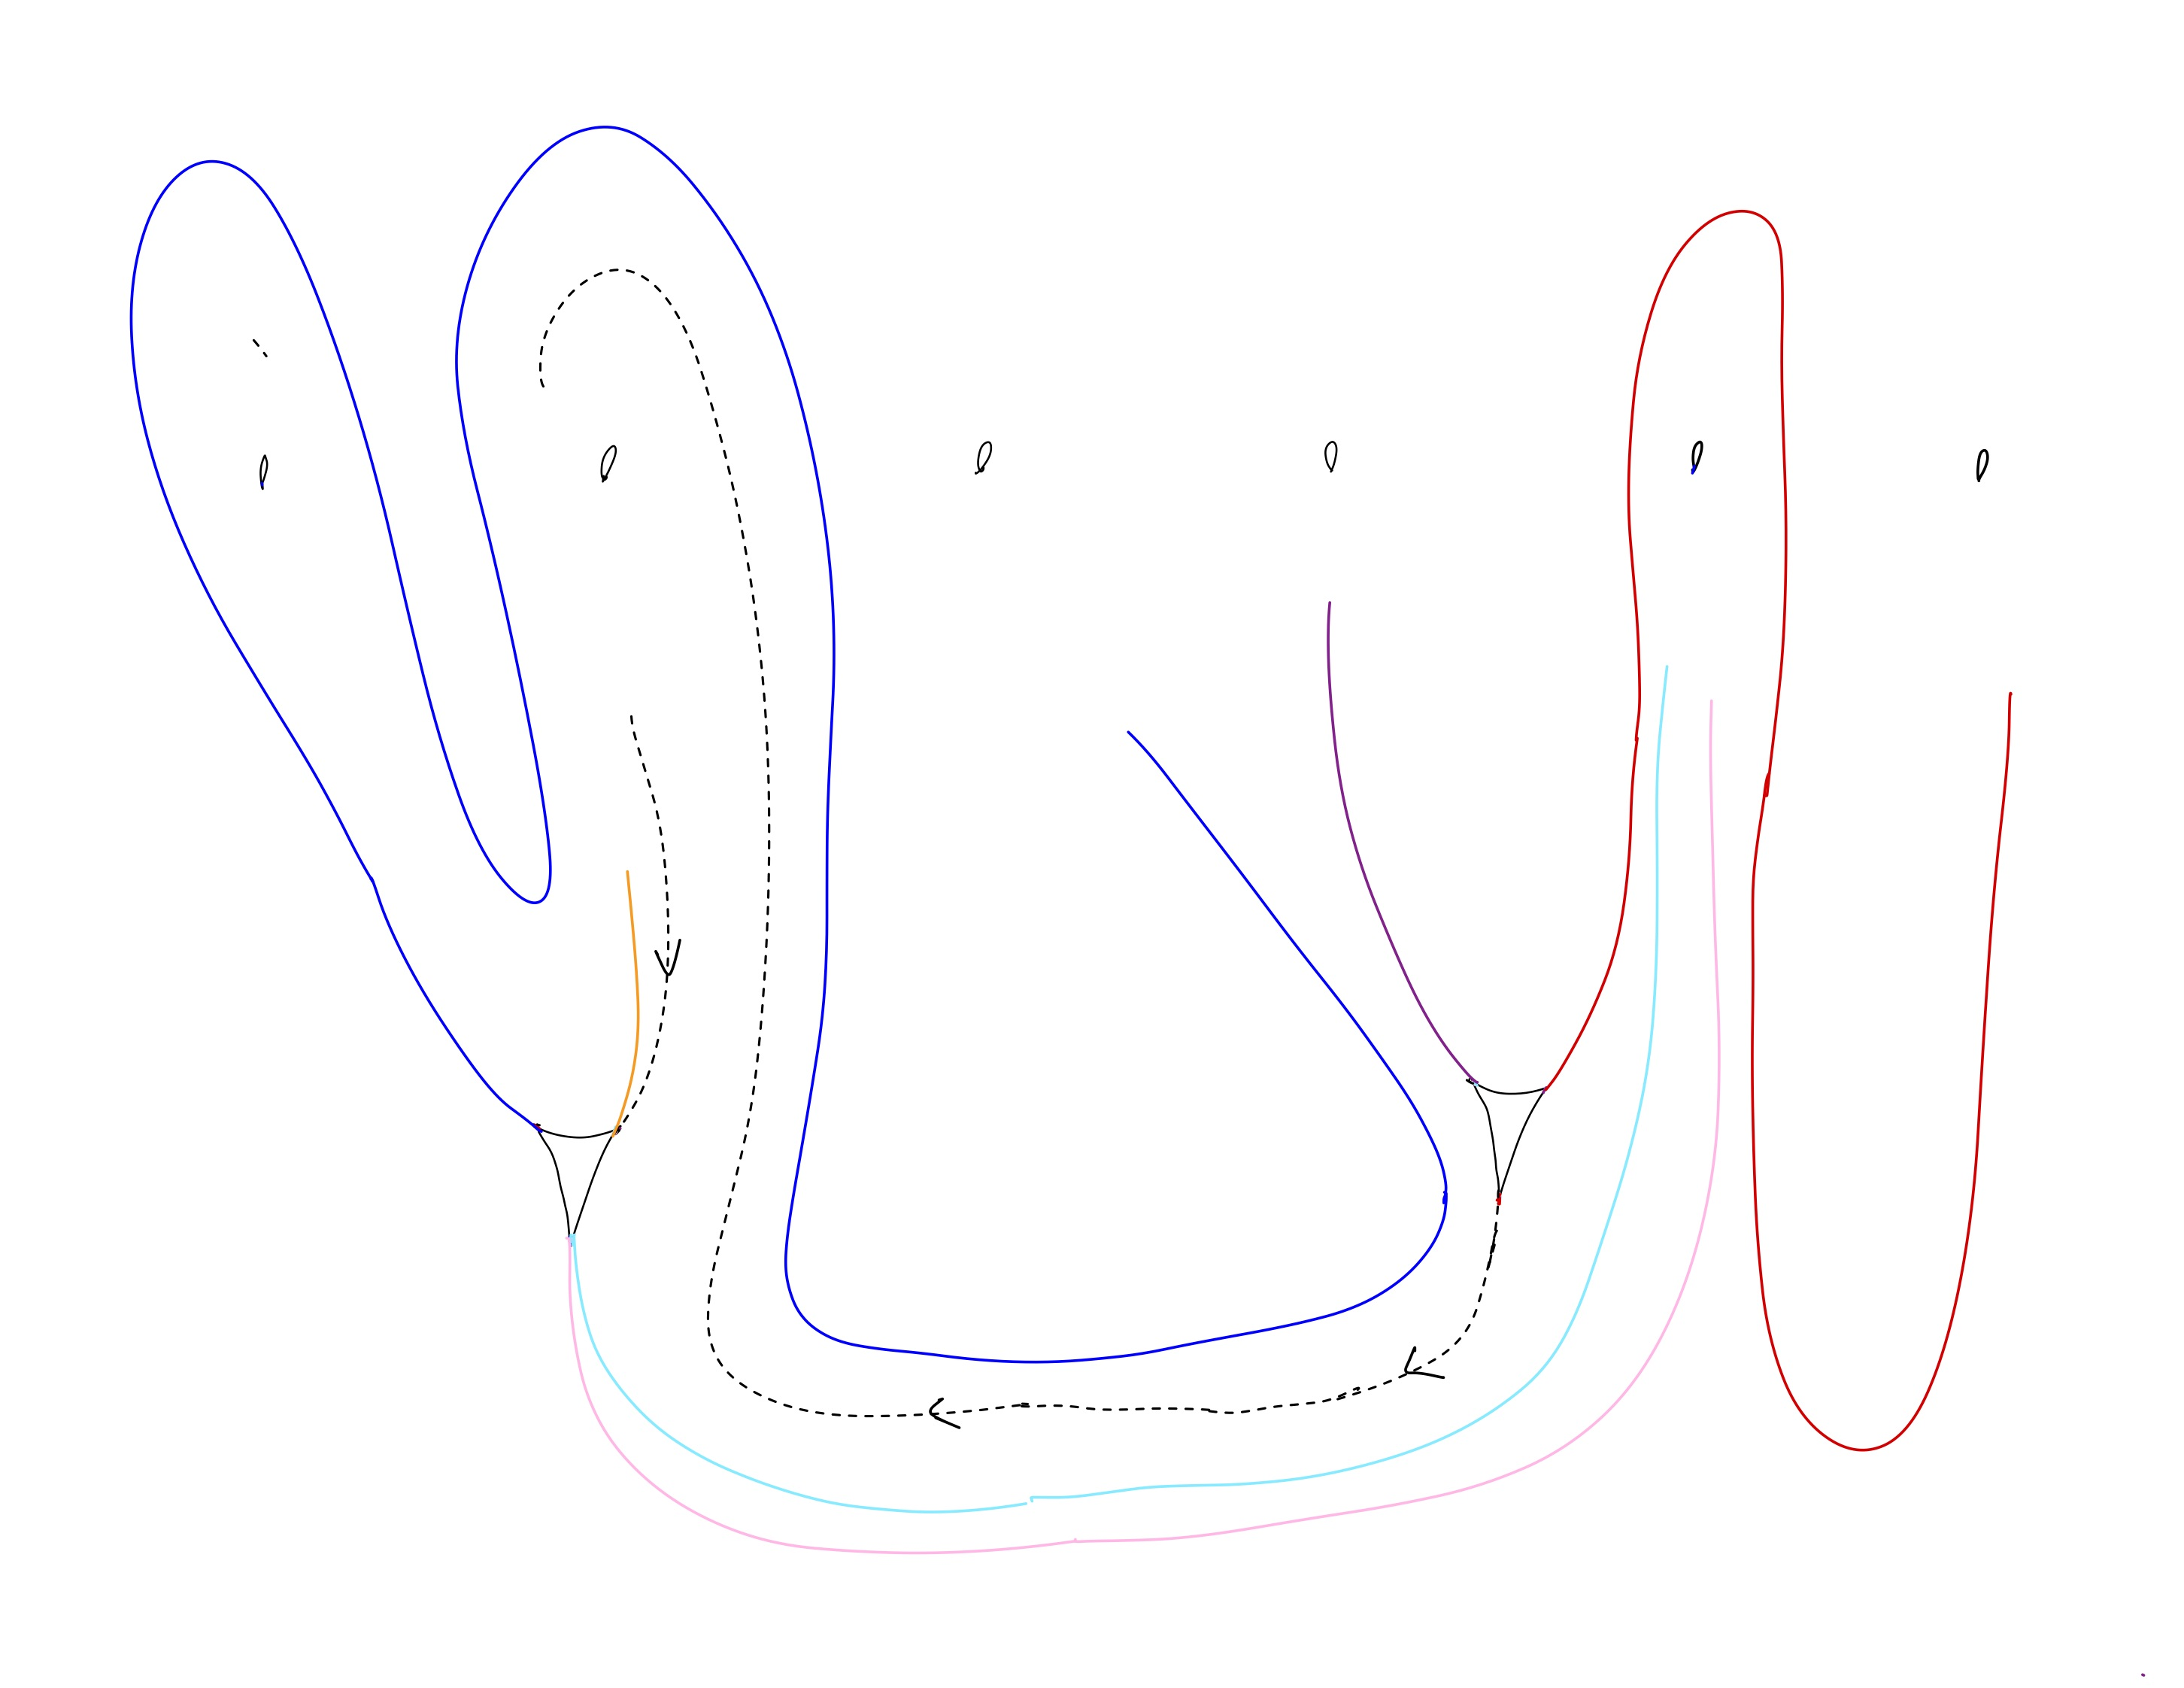
\includegraphics[width=\linewidth]{figures_case_analysis/track17_case_analysis/MMU-23.jpg}
    \caption{MMU23}
    \label{fig:MMU23}
\end{figure}

\begin{figure}[ht]
    \centering
    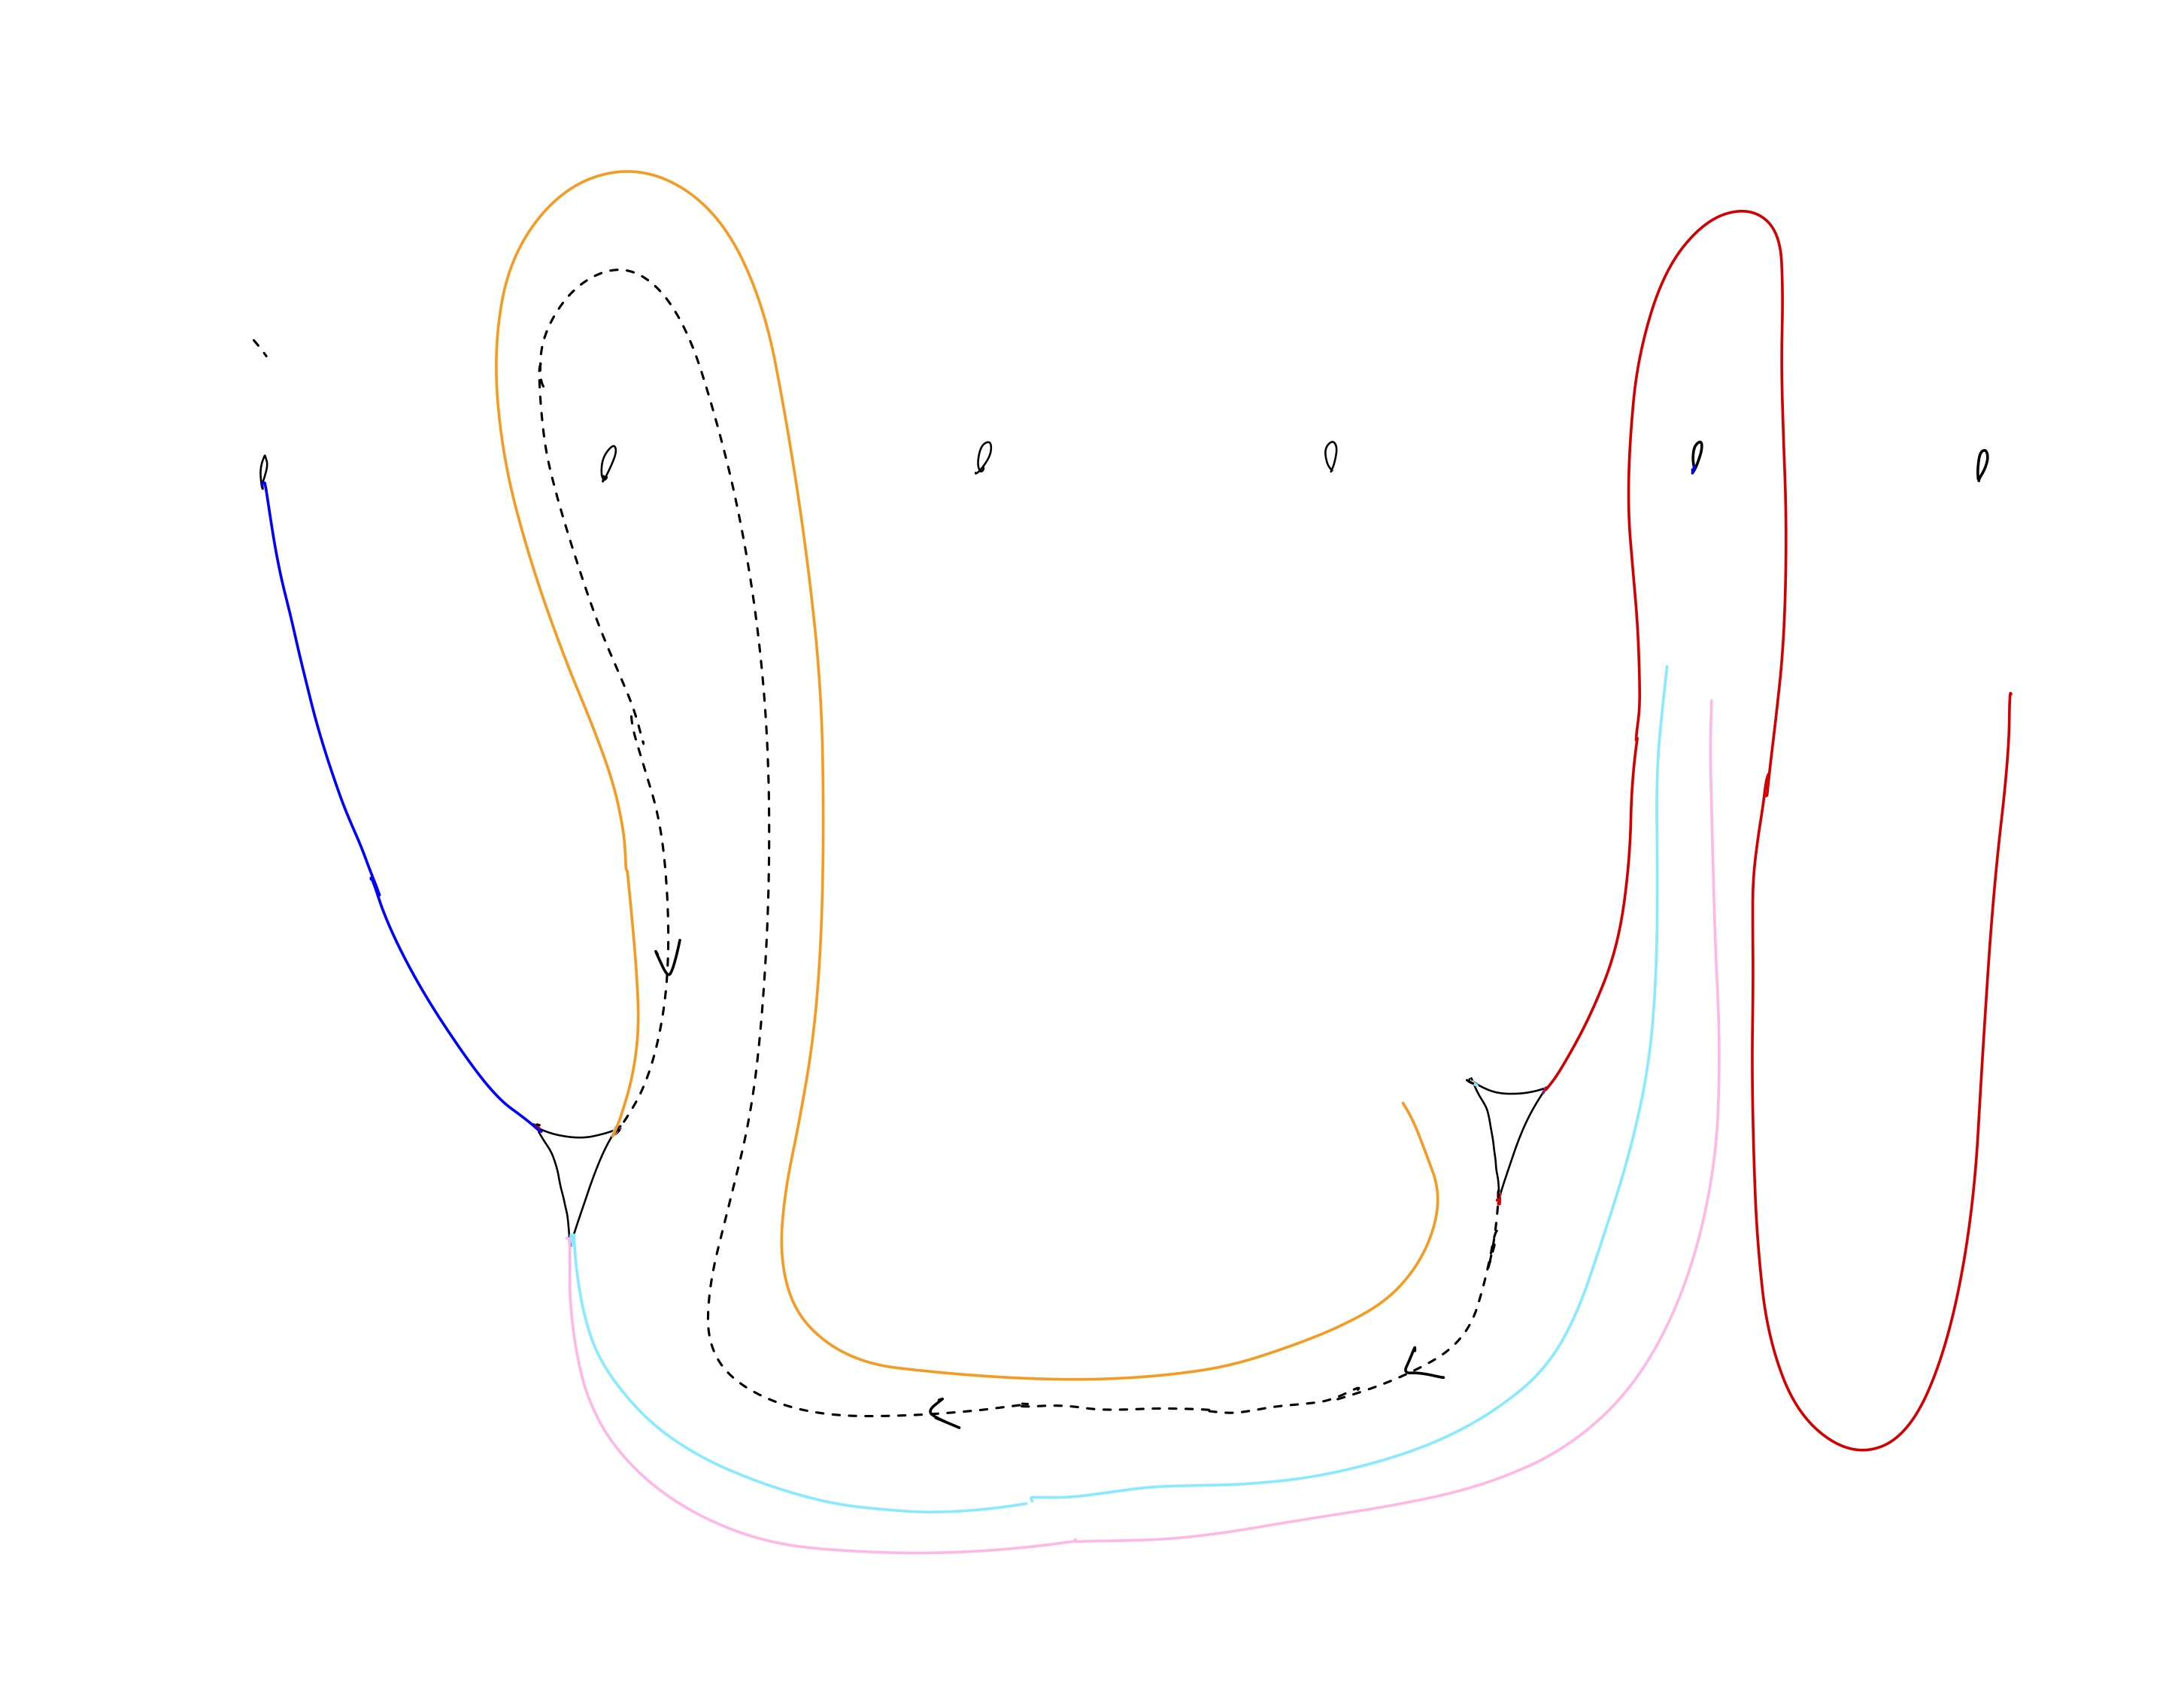
\includegraphics[width=\linewidth]{figures_case_analysis/track17_case_analysis/MMU-24.jpg}
    \caption{MMU24}
    \label{fig:MMU24}
\end{figure}
\clearpage

\begin{figure}[ht]
    \centering
    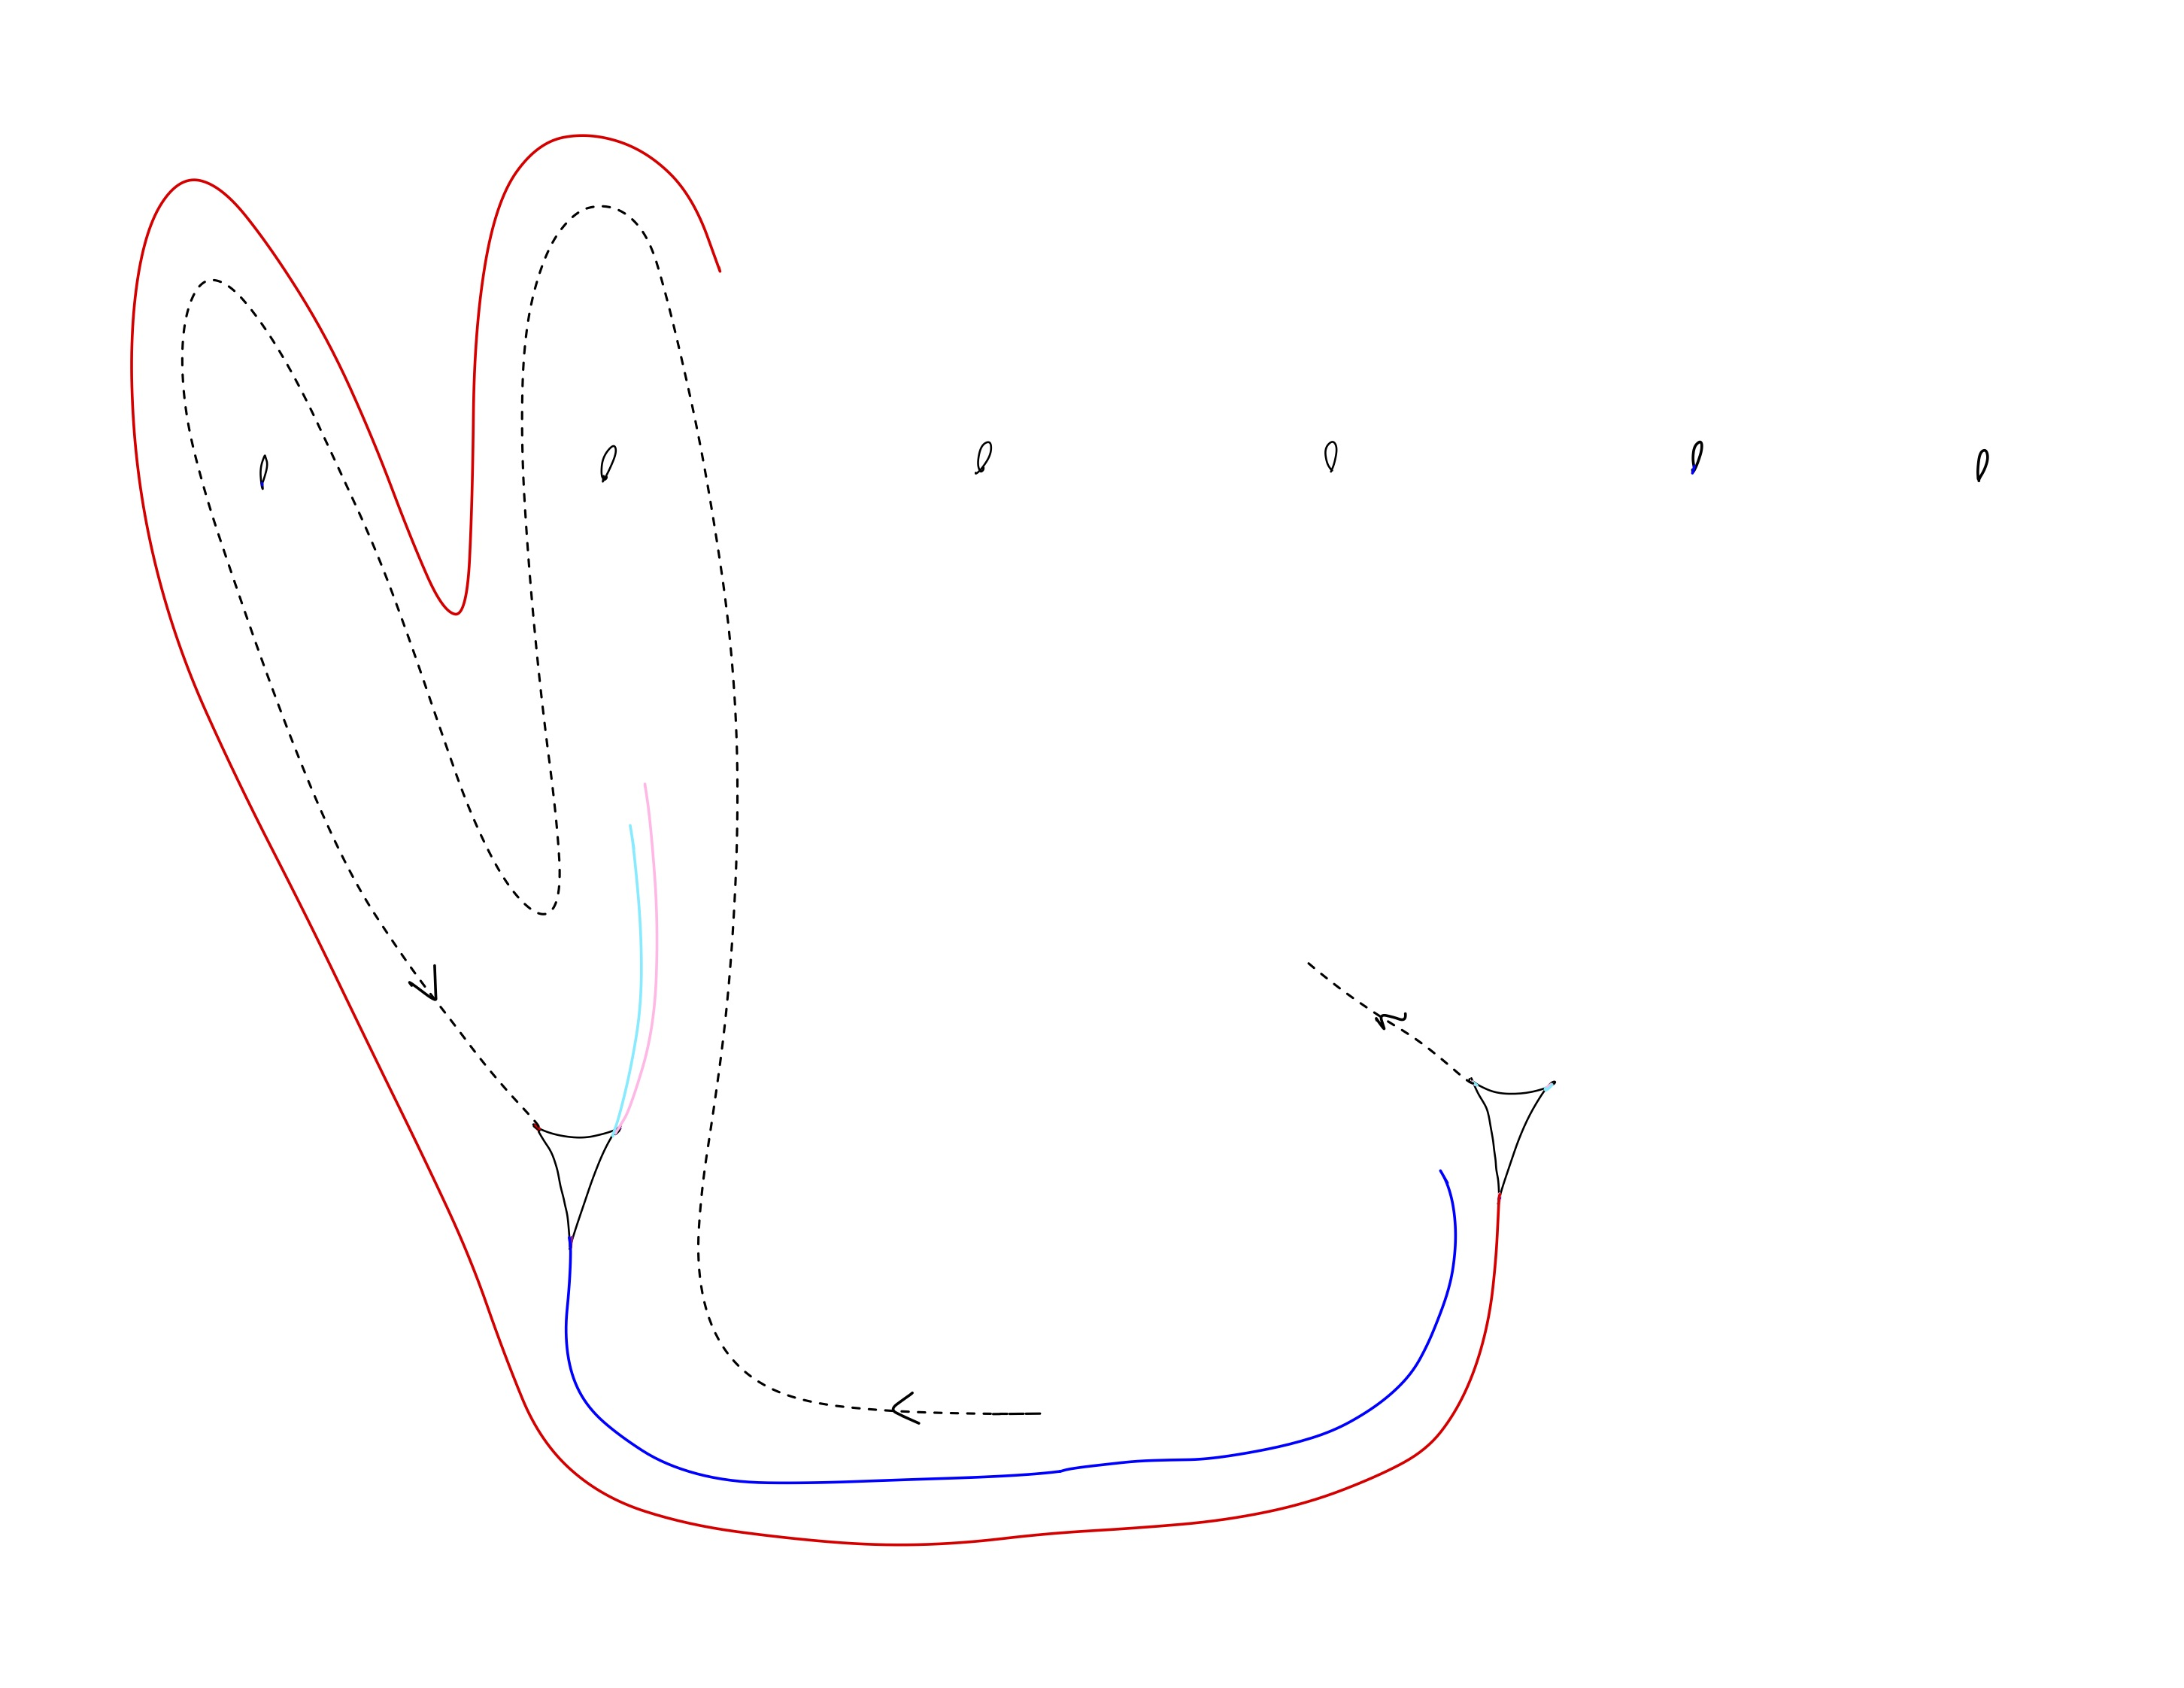
\includegraphics[width=\linewidth]{figures_case_analysis/track17_case_analysis/TKE-1.jpg}
    \caption{TKE1}
    \label{fig:TKE1}
\end{figure}

\begin{figure}[ht]
    \centering
    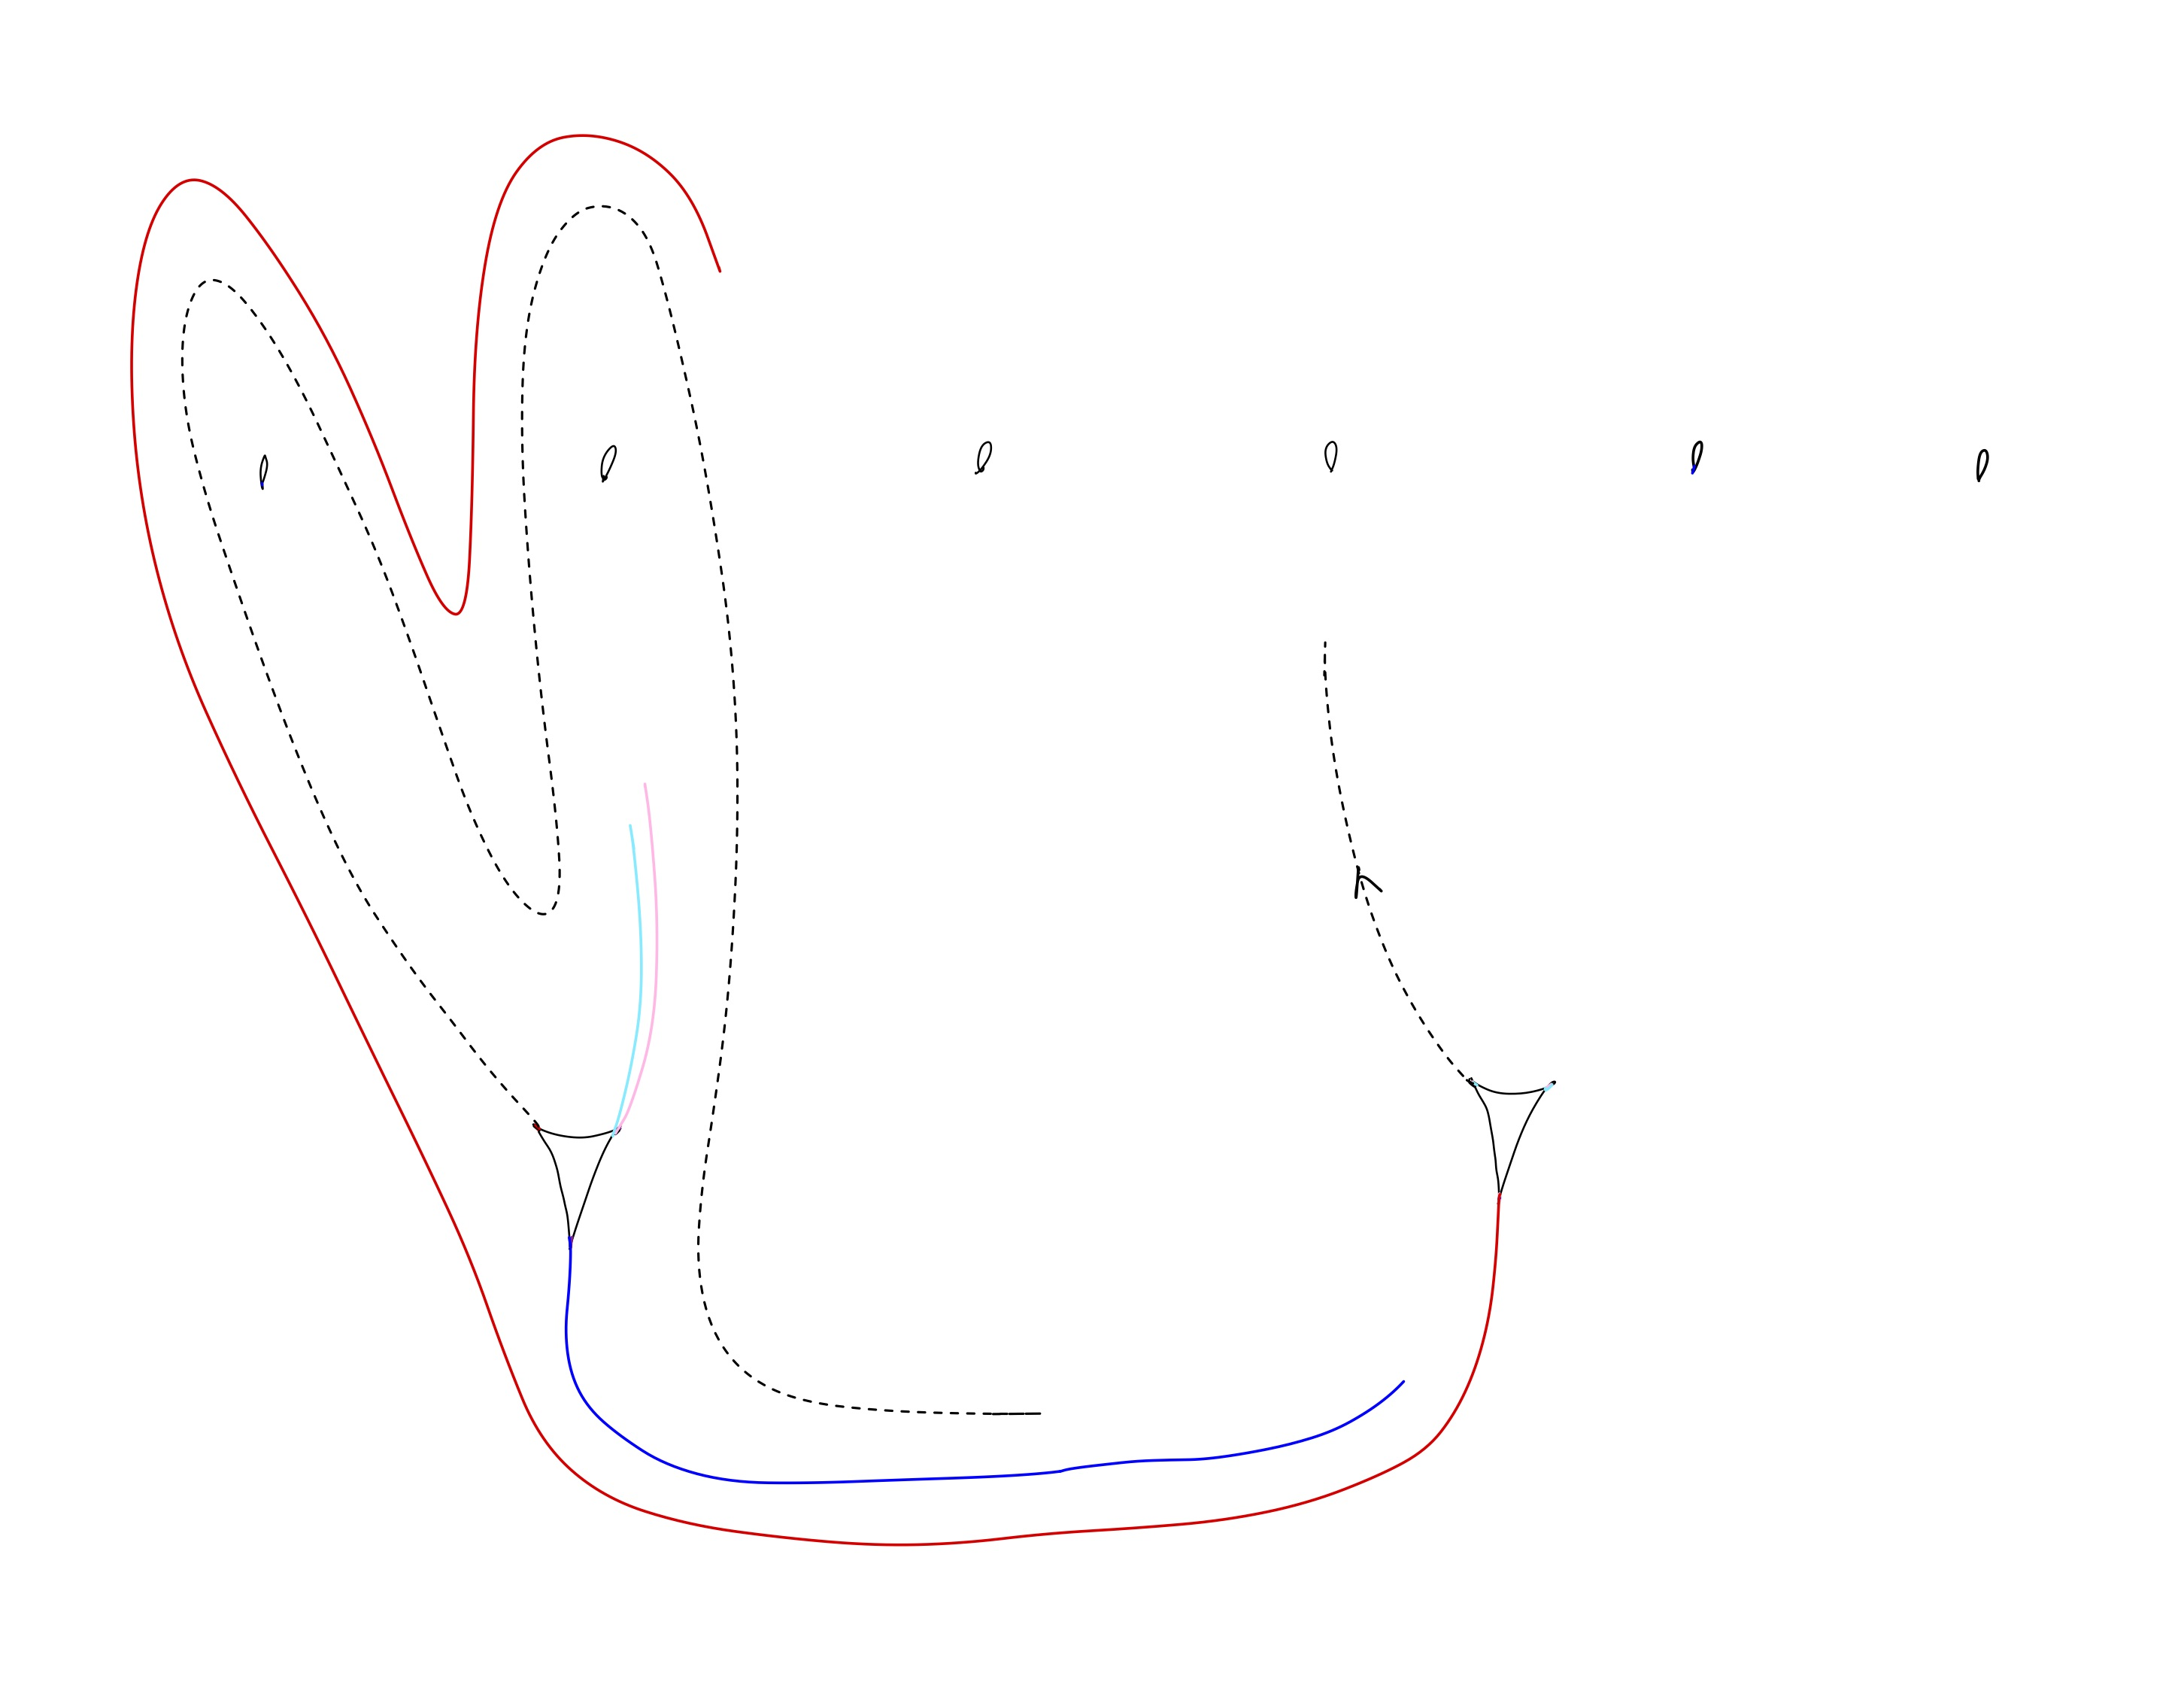
\includegraphics[width=\linewidth]{figures_case_analysis/track17_case_analysis/TKE-2.jpg}
    \caption{TKE2}
    \label{fig:TKE2}
\end{figure}

\begin{figure}[ht]
    \centering
    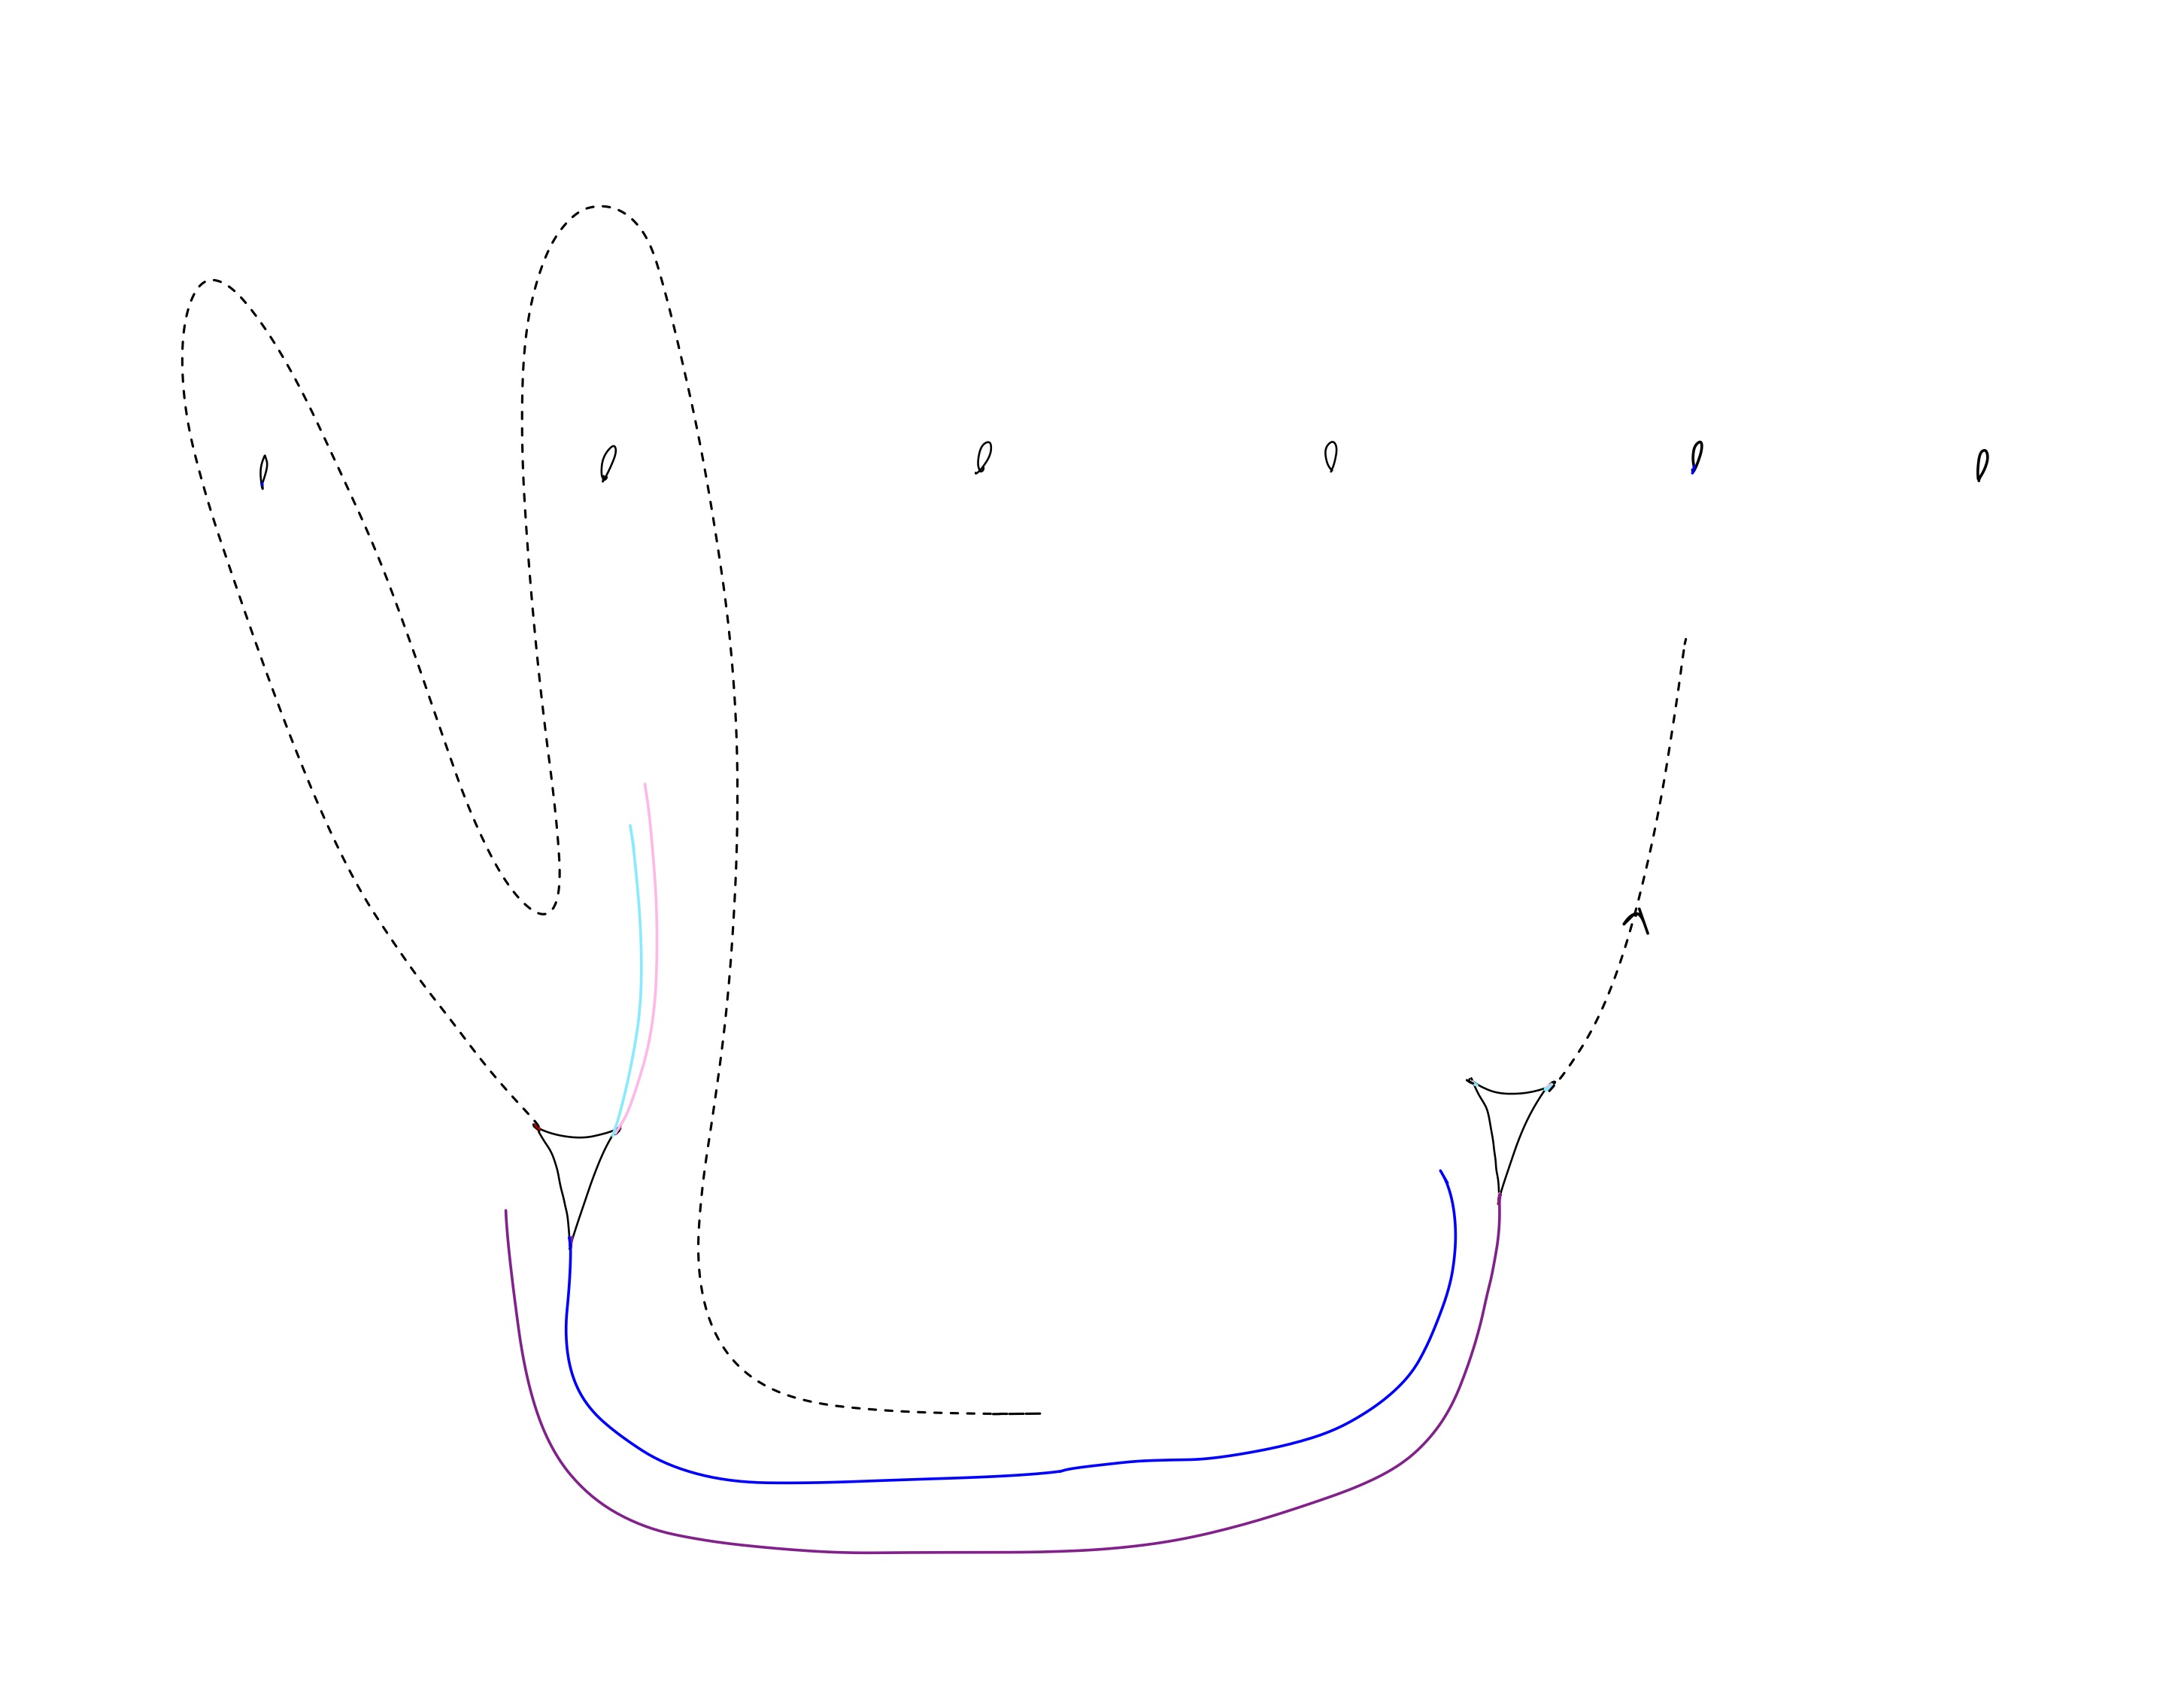
\includegraphics[width=\linewidth]{figures_case_analysis/track17_case_analysis/TKE-3.jpg}
    \caption{TKE3}
    \label{fig:TKE3}
\end{figure}
\clearpage

\begin{figure}[ht]
    \centering
    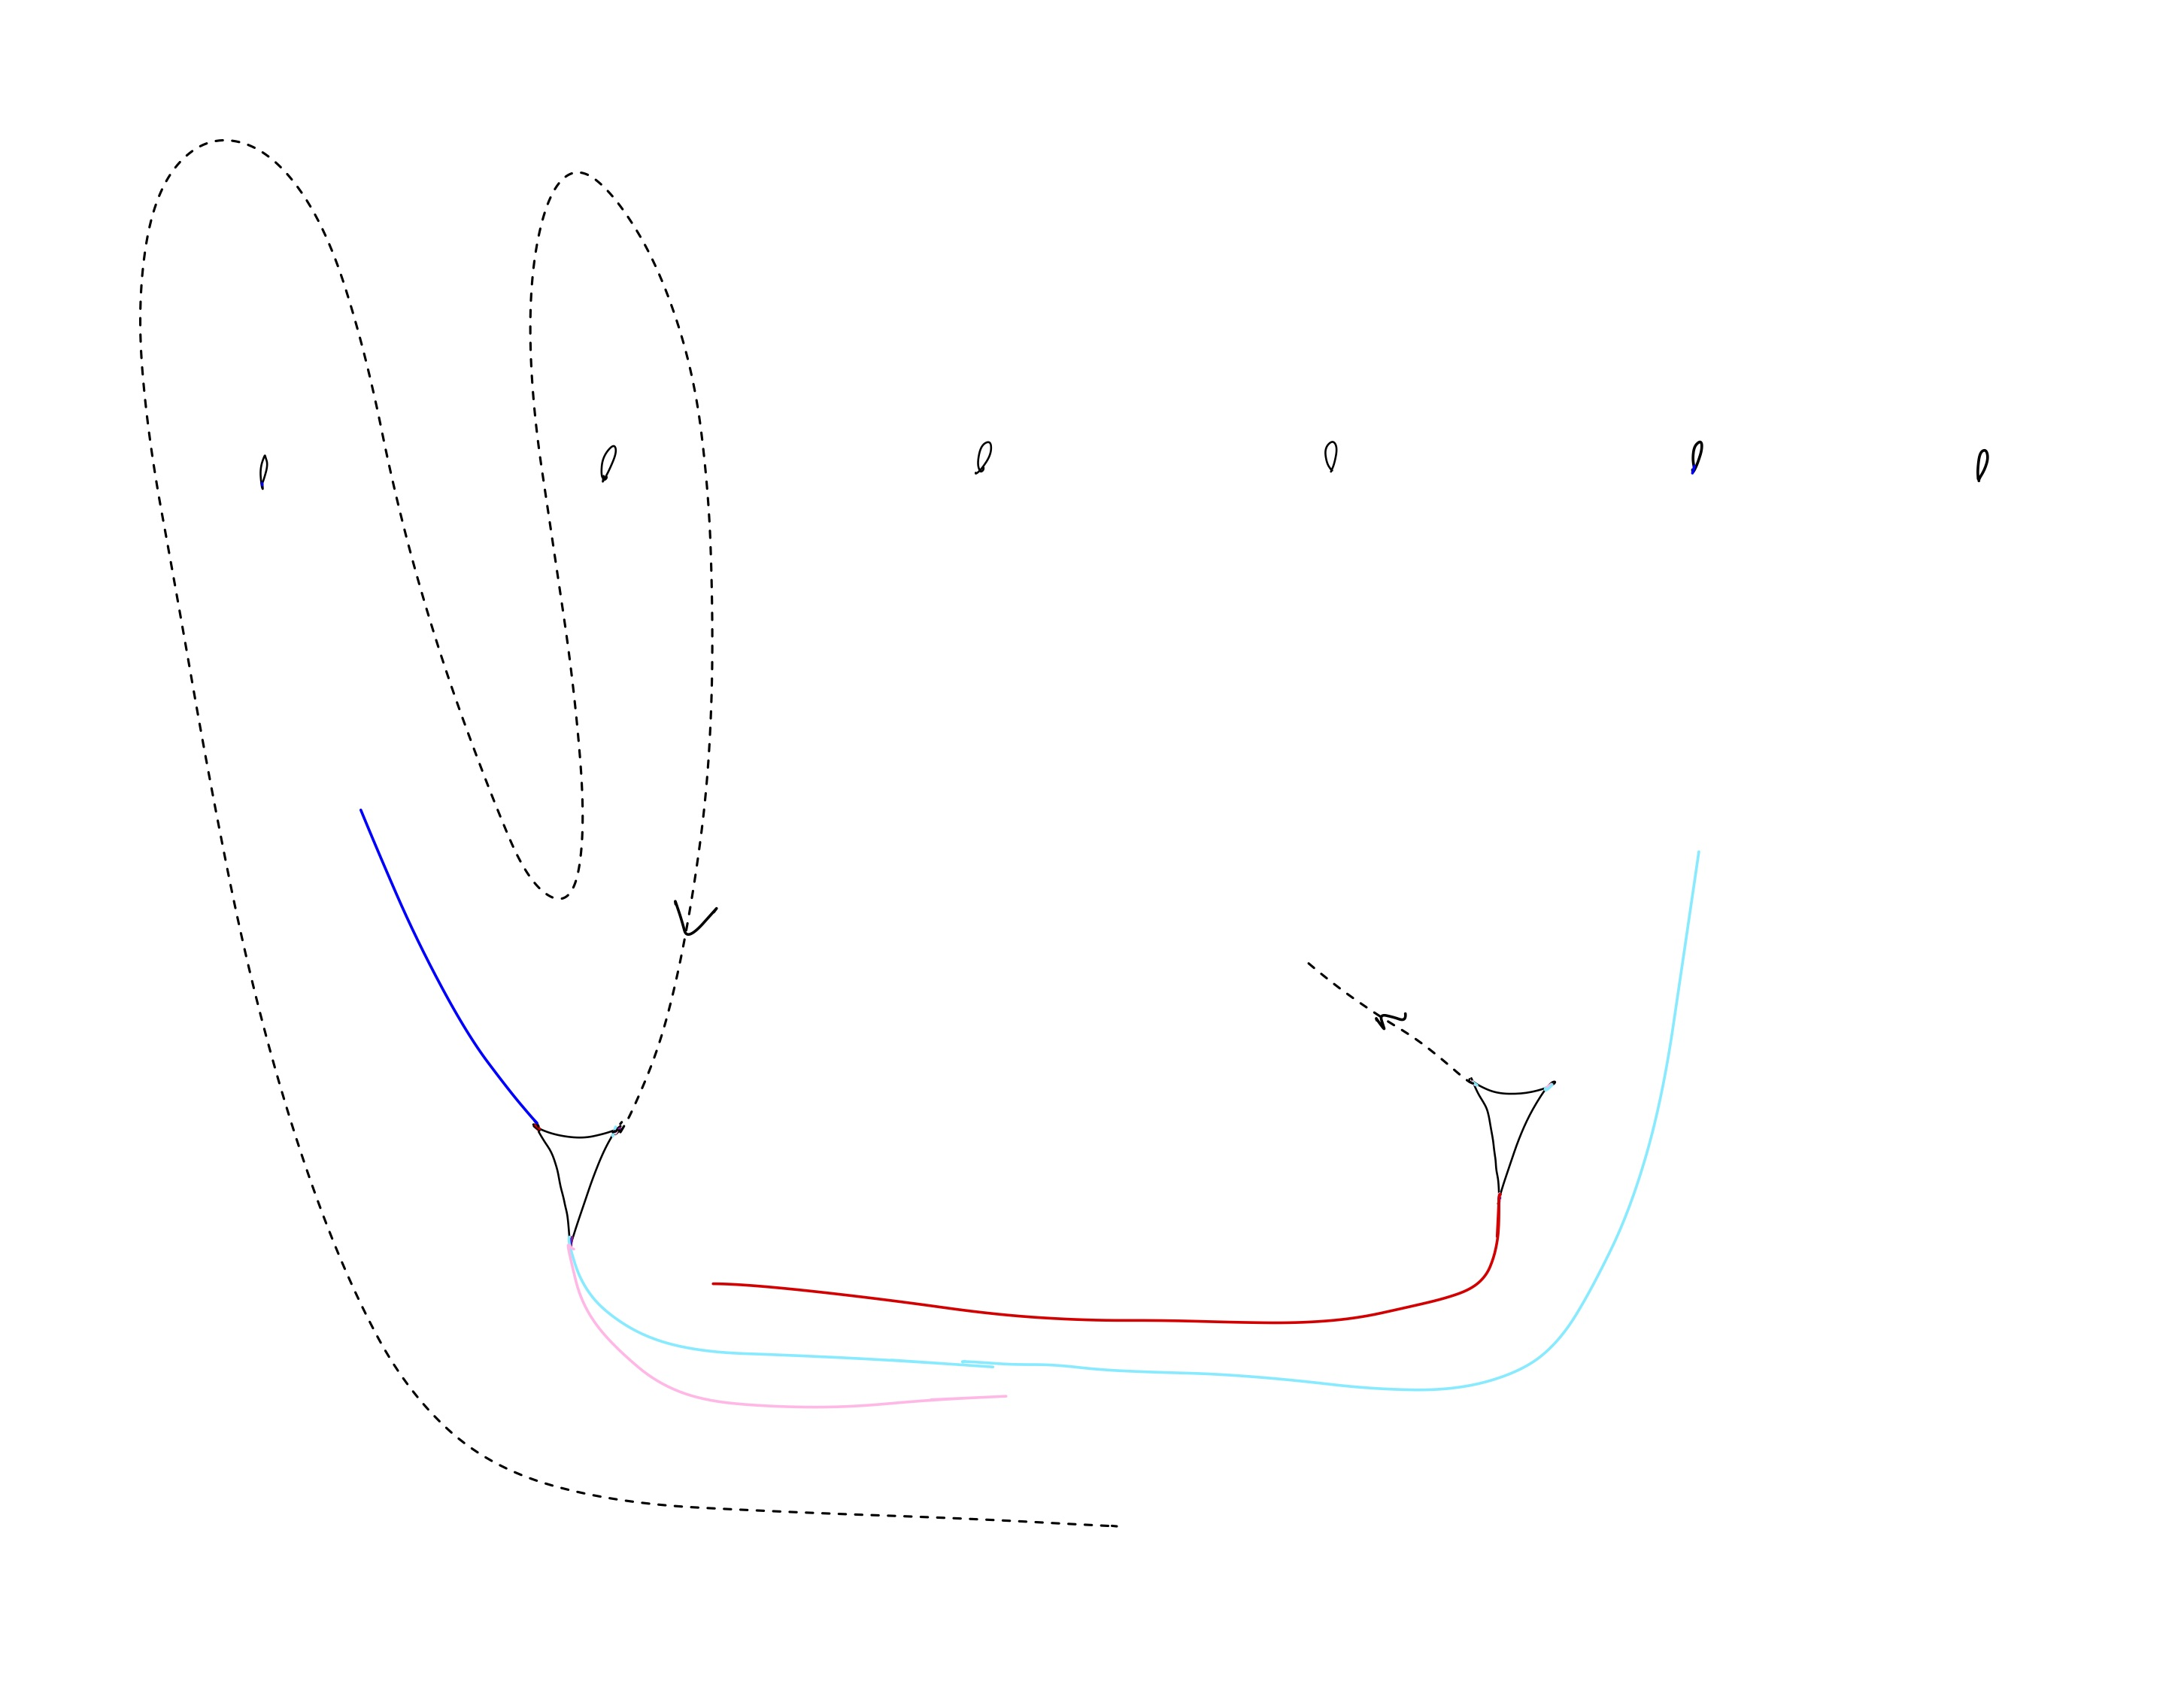
\includegraphics[width=\linewidth]{figures_case_analysis/track17_case_analysis/RKD-1.jpg}
    \caption{RKD1}
    \label{fig:RKD1}
\end{figure}

\begin{figure}[ht]
    \centering
    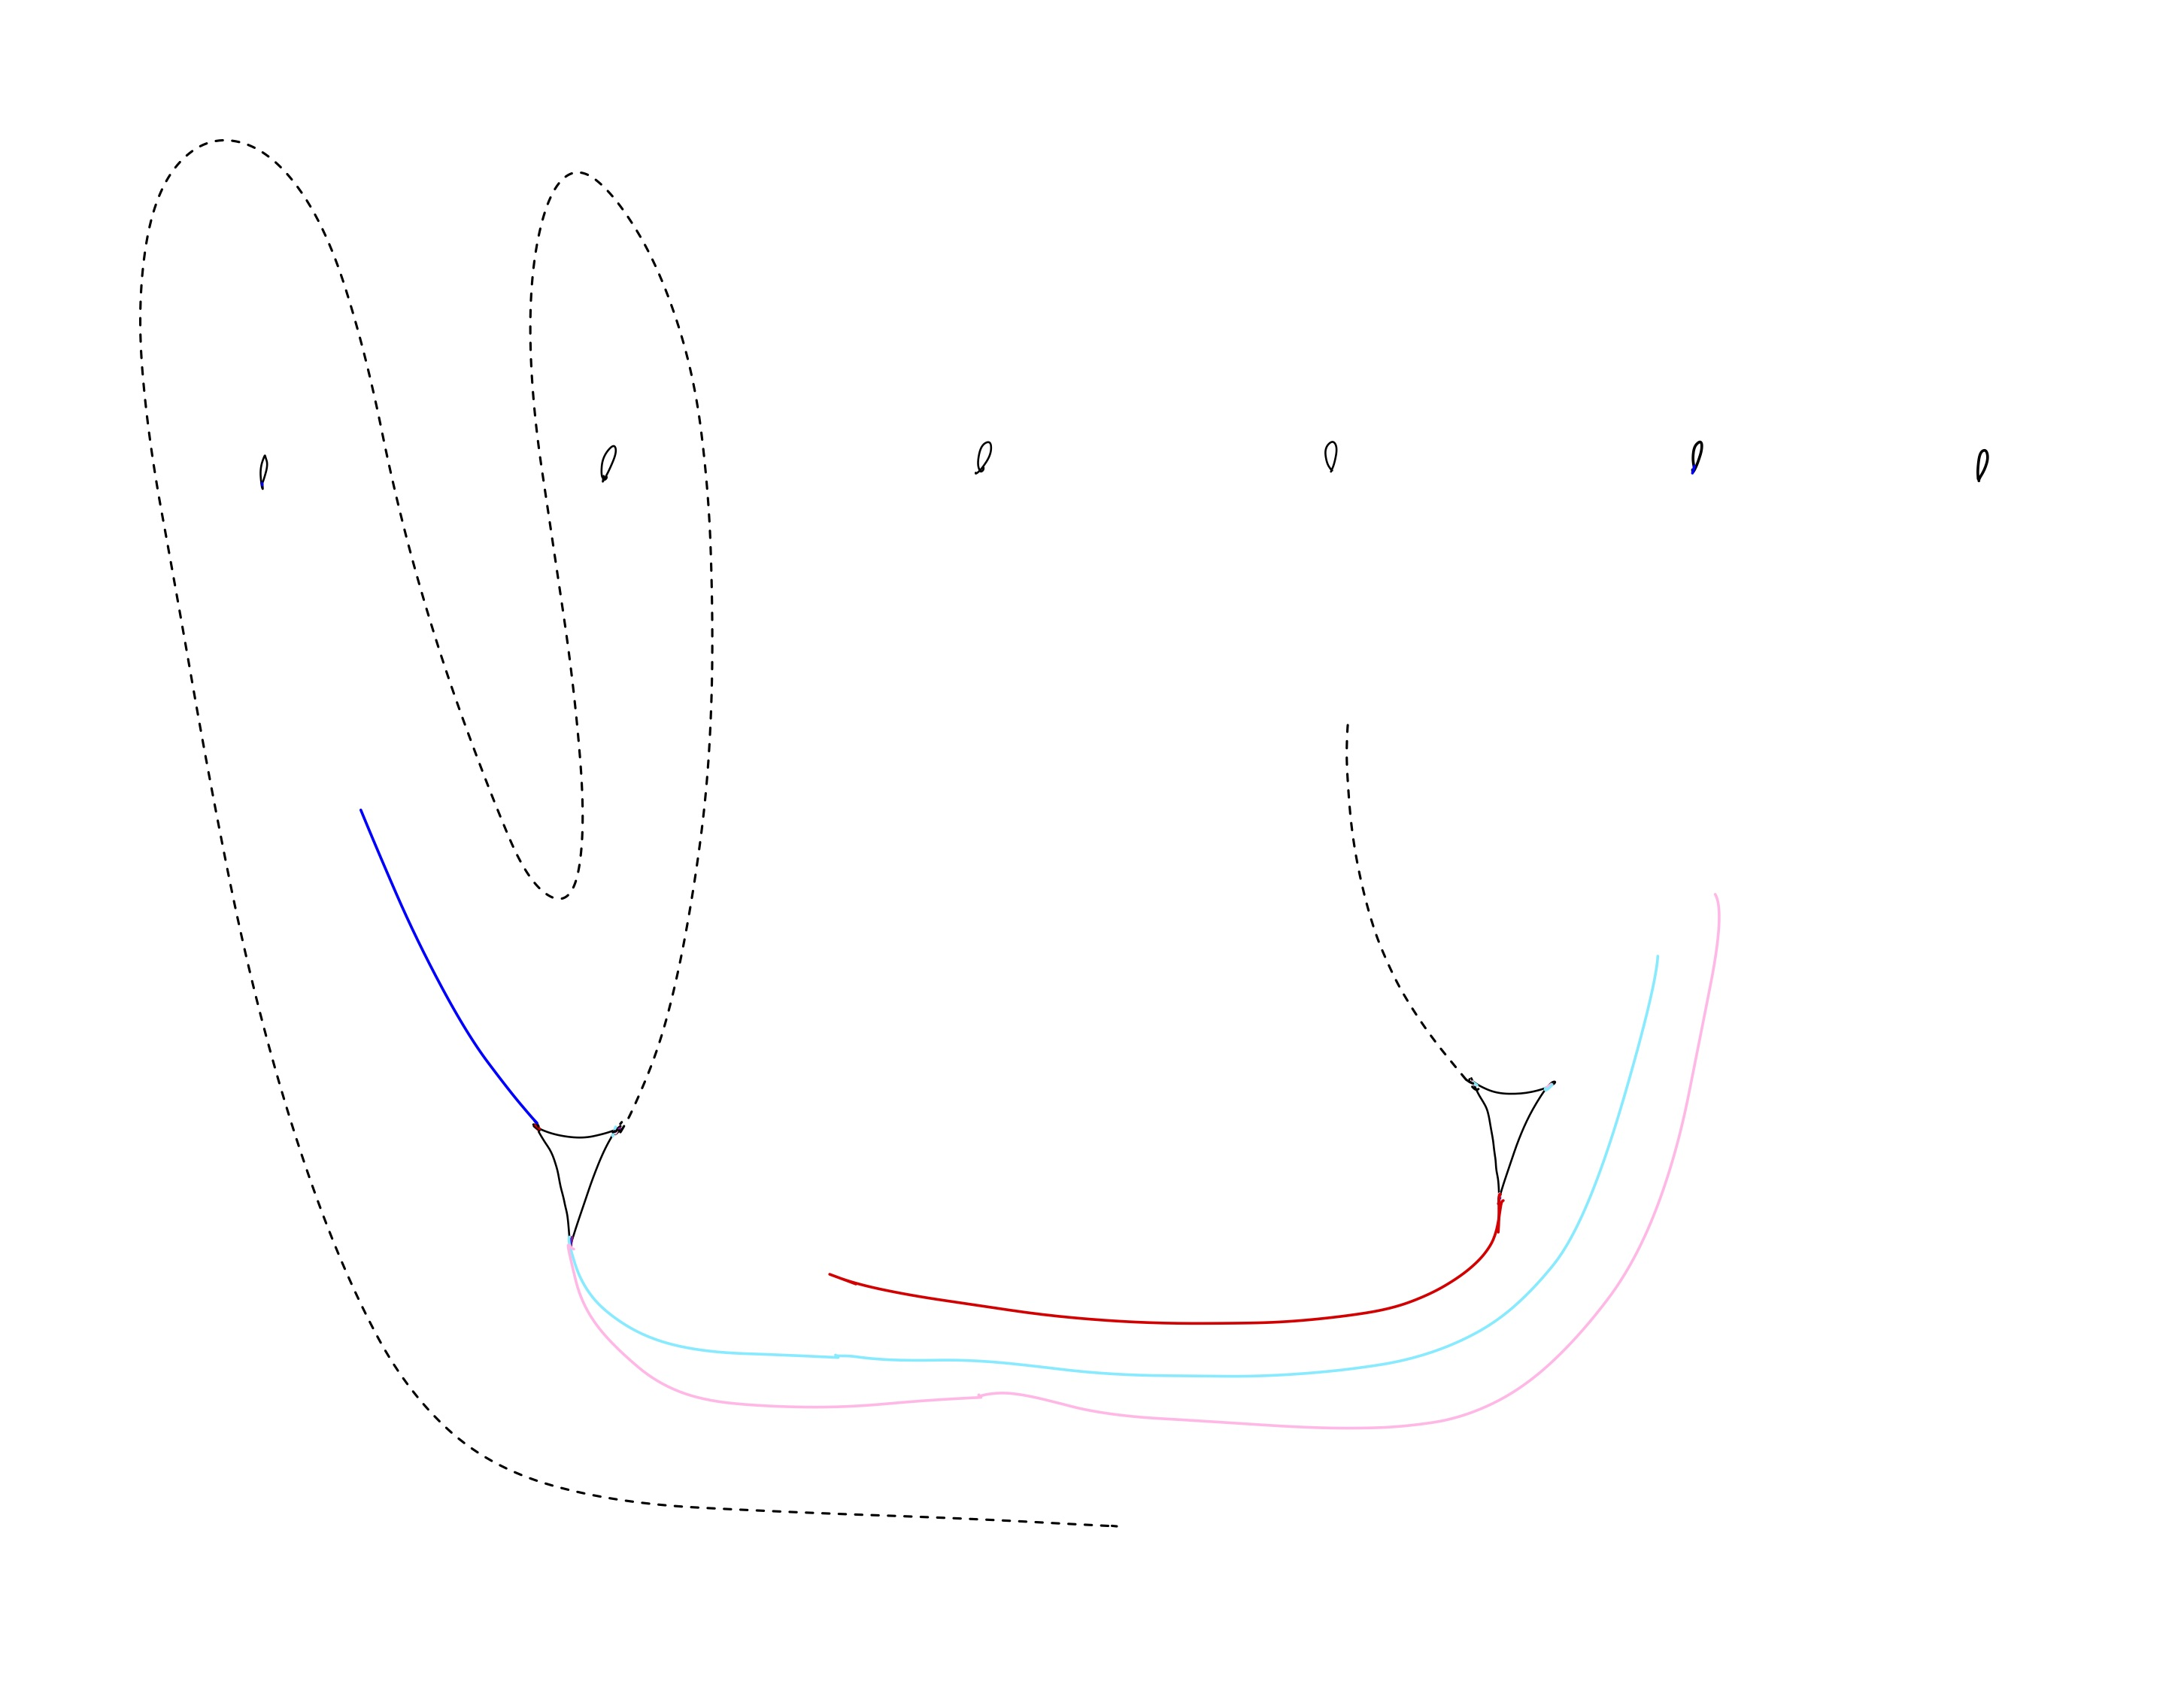
\includegraphics[width=\linewidth]{figures_case_analysis/track17_case_analysis/RKD-2.jpg}
    \caption{RKD2}
    \label{fig:RKD2}
\end{figure}

\begin{figure}[ht]
    \centering
    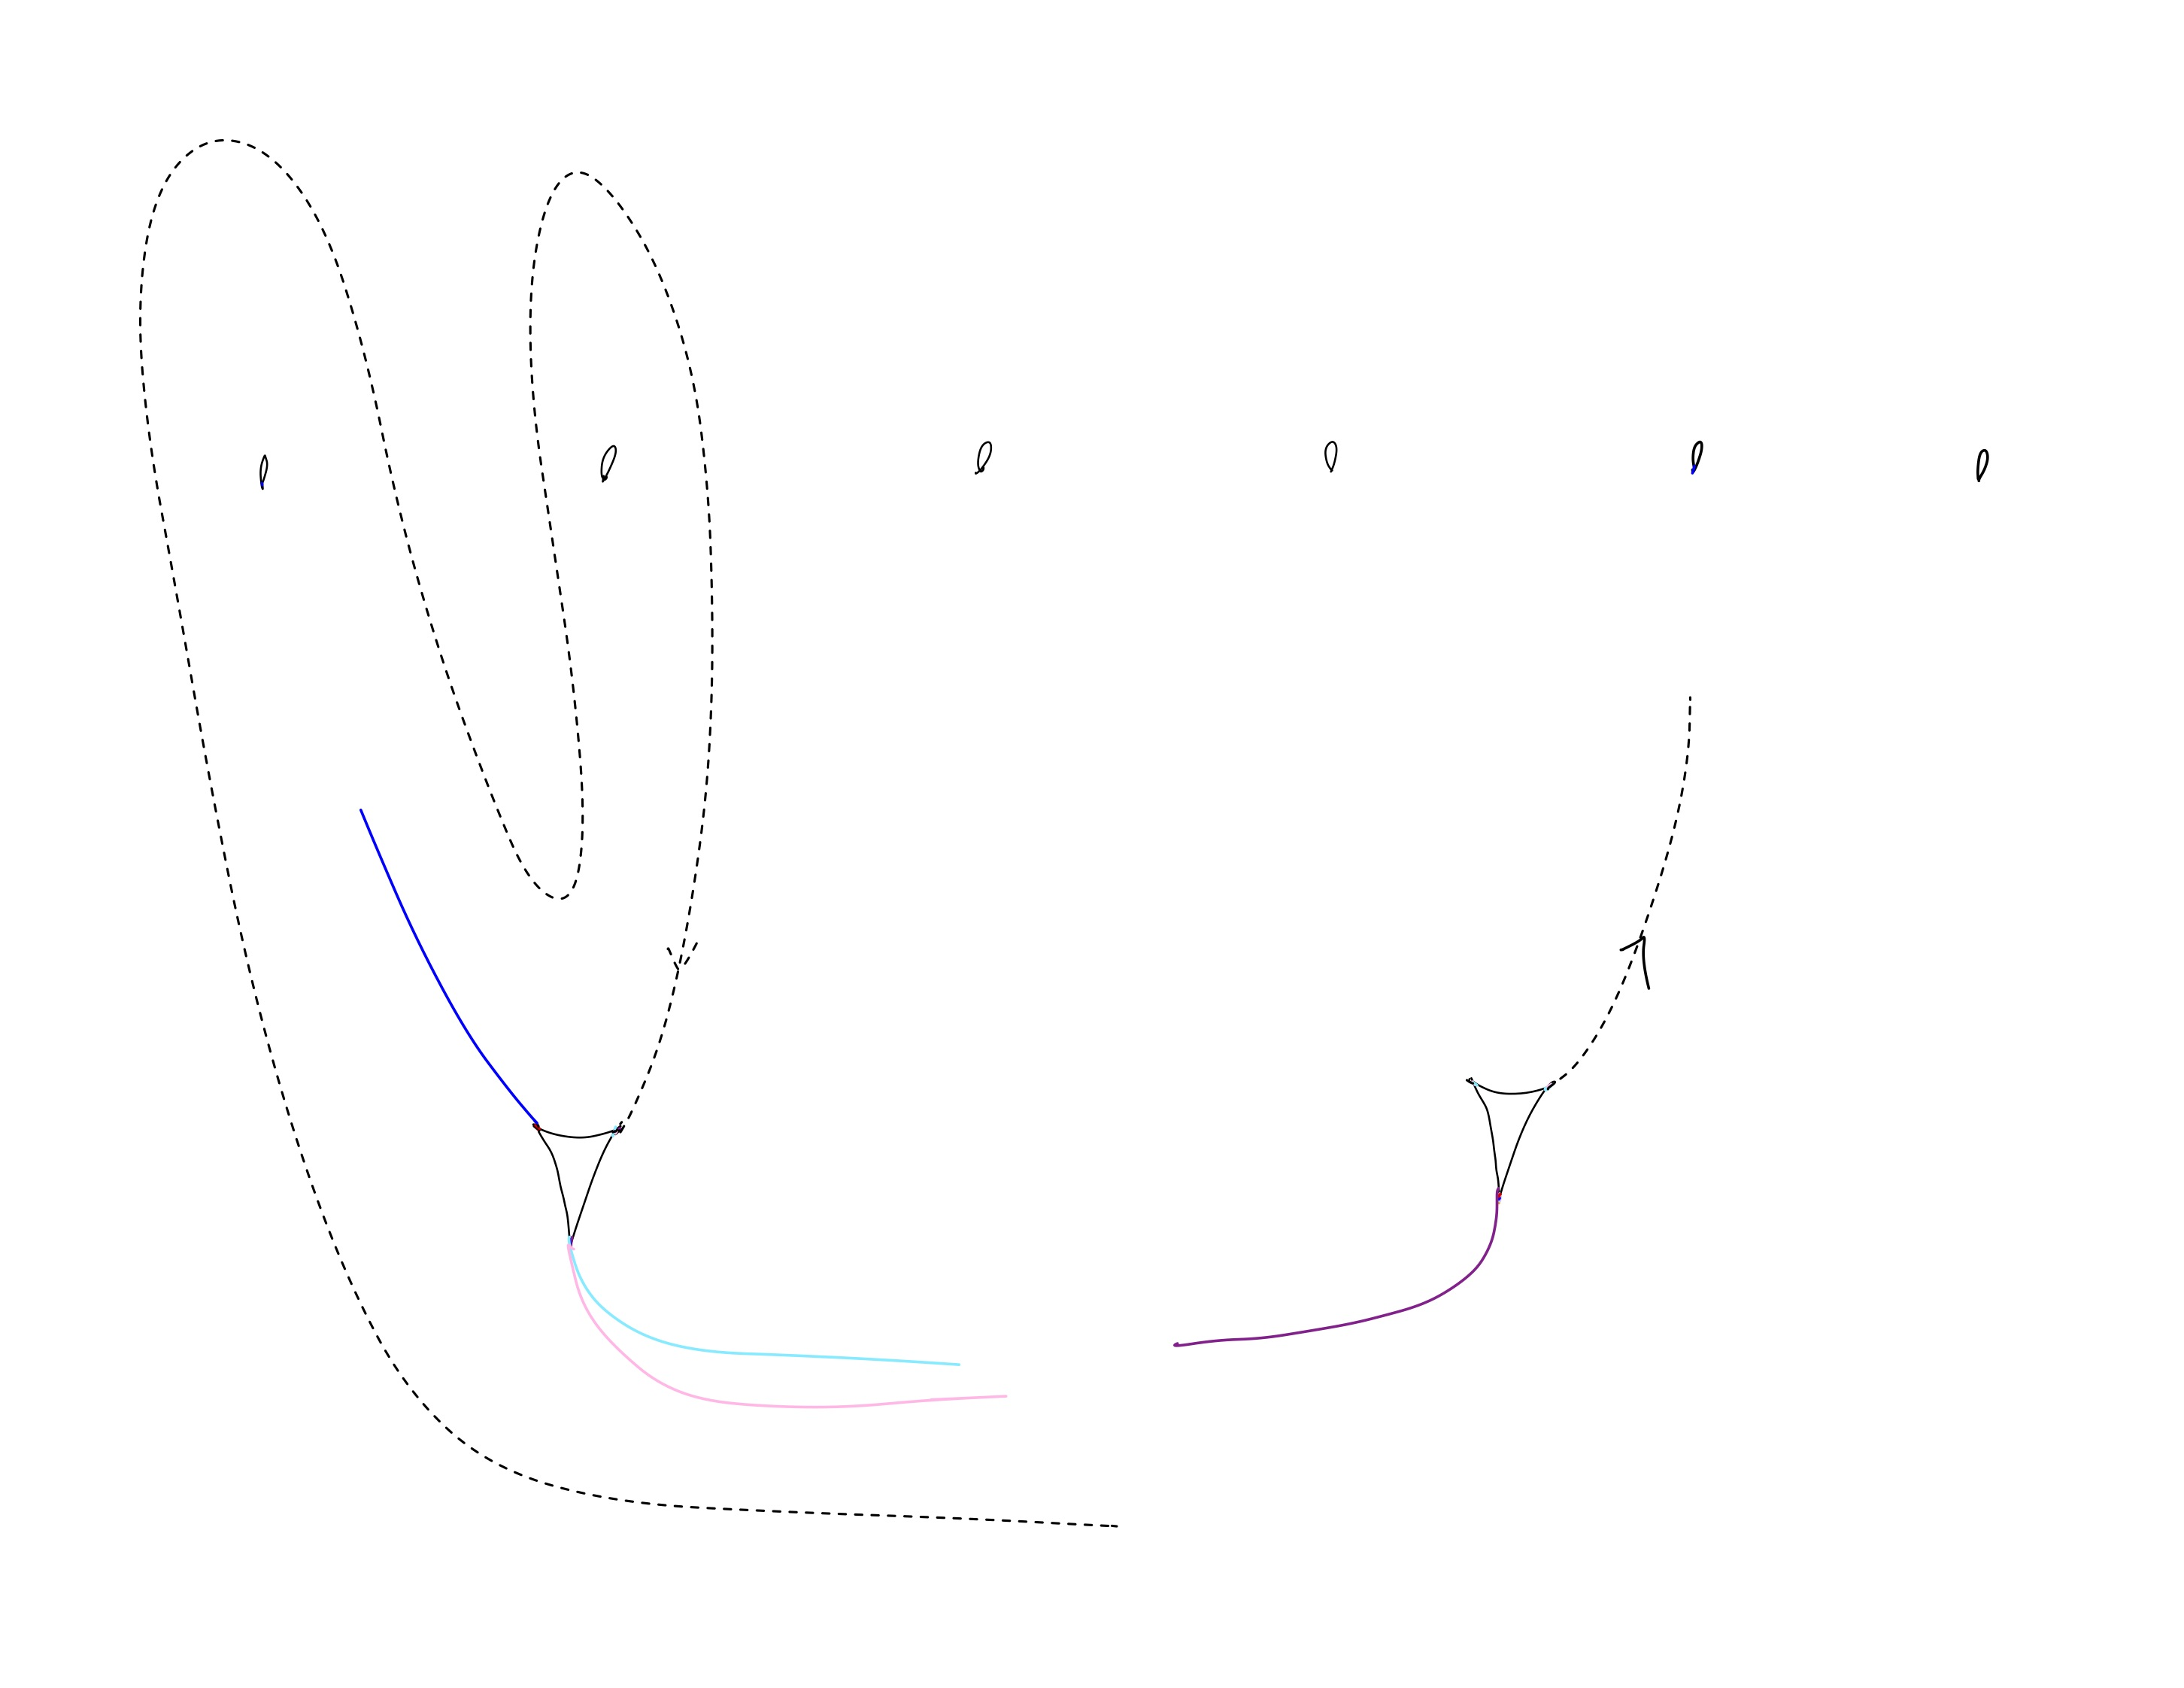
\includegraphics[width=\linewidth]{figures_case_analysis/track17_case_analysis/RKD-3.jpg}
    \caption{RKD3}
    \label{fig:RKD3}
\end{figure}

\begin{figure}[ht]
    \centering
    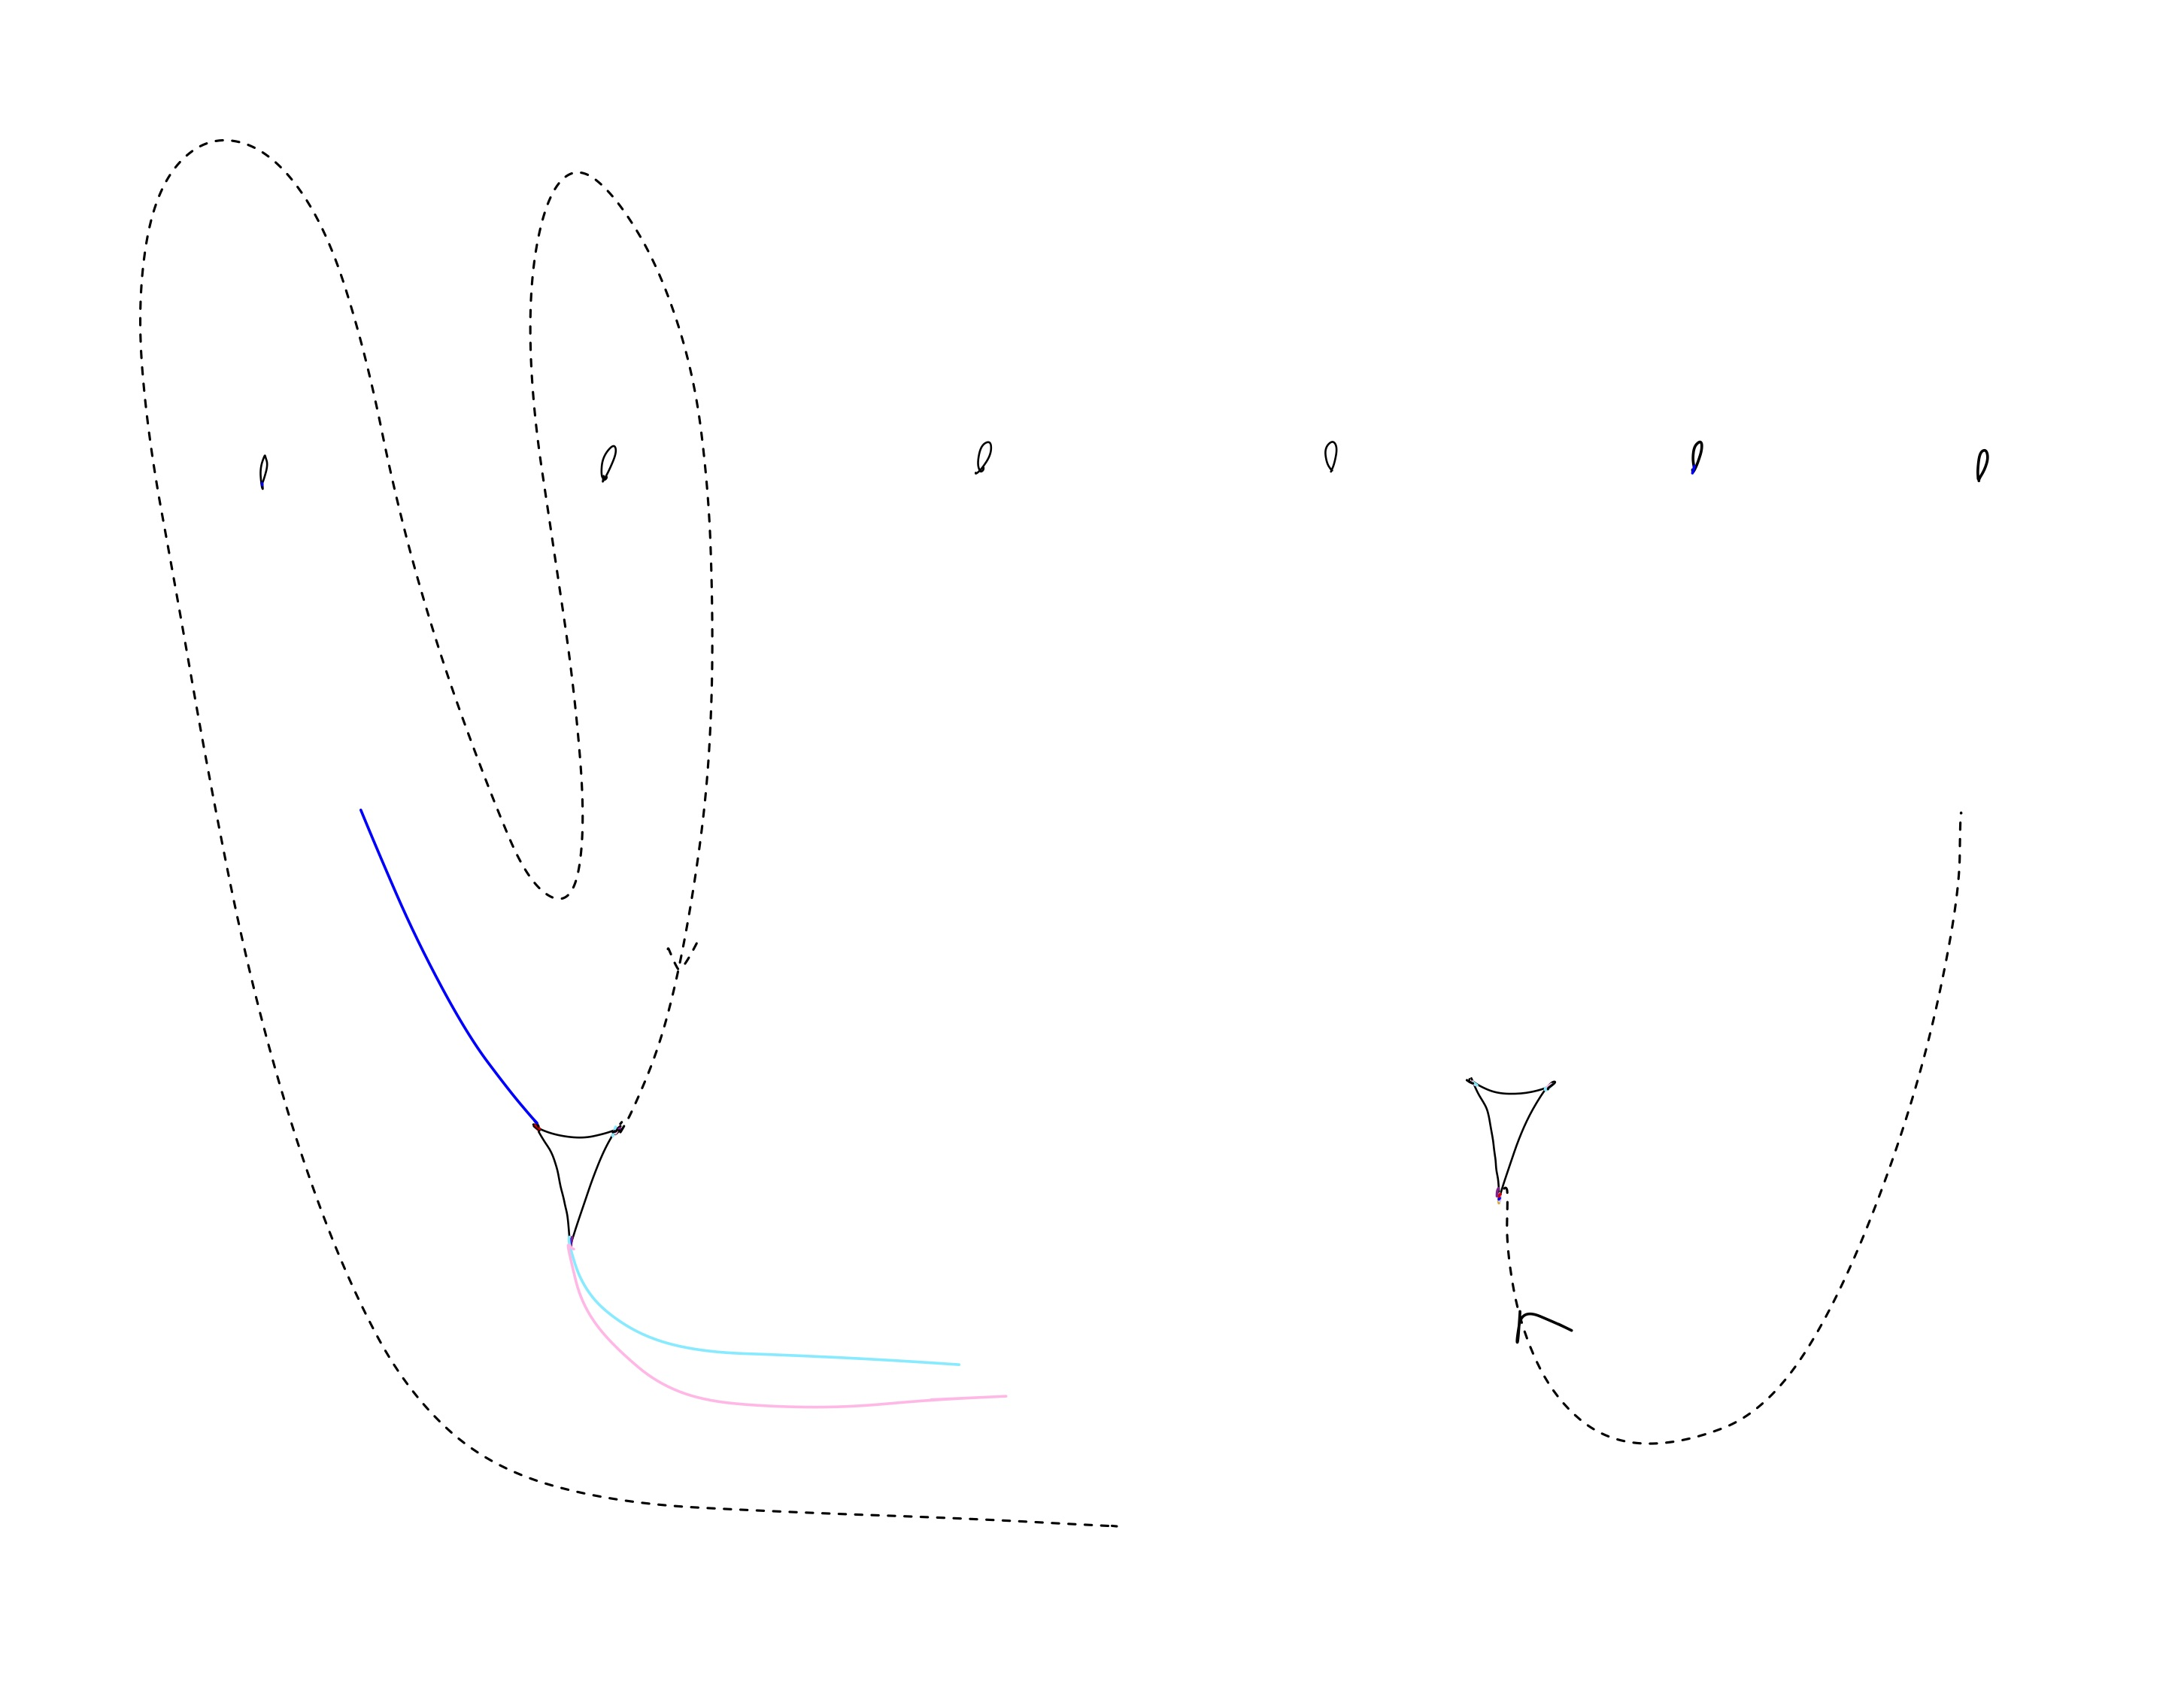
\includegraphics[width=\linewidth]{figures_case_analysis/track17_case_analysis/RKD-4.jpg}
    \caption{RKD4}
    \label{fig:RKD4}
\end{figure}
